% !TeX spellcheck = de_DE
% ===================================================================================
% P R E A M B E L 
% ===================================================================================
% Basic document settings -----------------------------------------------------------
\documentclass[11pt, twoside, a4paper]{book}		% option draft for no images and overfull hbox markers
\linespread{1.3}\selectfont							% use one and a half line spaces
%\renewcommand{\familydefault}{\sfdefault}			% sets file in sans serif
%\setlength{\marginparwidth}{0pt}					% removes margin notes area O_o
%\setlength{\parskip}{1.5ex plus 0.5ex minus 0.2ex}	% https://en.wikibooks.org/wiki/LaTeX/Page_Layout#Widows_and_orphans
\AtBeginDocument{\setlength{\parindent}{2em}}		% parindent 2 em units for new paragraph
%\usepackage{indentfirst}							% use if first paragraph should be indented
\usepackage[pass]{geometry}							% ’pass’ disregards the package layout, so the original ’book’ layout is memorized here
\usepackage{layout}									% show layout on page 1
%\usepackage{showframe}								% show frame on pages
%\usepackage{url}									% loaded internally by hyperref
%\usepackage{booktabs}								% Nicely formatted tables
%\usepackage{topcapt}								% Be able to put captions above tables 
%\usepackage{chngpage}								% Be able to change margins on the fly for big tables
%\usepackage{longtable}								% For tables that go over sereral pages
\usepackage[utf8]{inputenc}							% this is needed for umlauts
\usepackage[T1]{fontenc}							% this is needed for correct output of umlauts in pdf
\usepackage[ngerman, showlanguages]{babel}			% set document language to new german
\usepackage[german=swiss]{csquotes}					% enquote{} makes quoting in swiss german easy
\usepackage{pdflscape}								% https://en.wikibooks.org/wiki/LaTeX/Page_Layout#cite_ref-4
\usepackage{longtable}								% a multi-page environment for tabular
\usepackage{listings}								% for R code snippets
\usepackage{graphicx}								% needed for graphics
\renewcommand{\textfraction}	{.001}				% minimum fraction text per side
\renewcommand{\topfraction}		{.999}				% fraction of float on top page
\renewcommand{\bottomfraction}	{.999}				% fraction of float on bottum page
\usepackage[hang, bottom]{footmisc}					% footnotes are indented and always on bottom of the page
\setlength{\footnotesep}{.9\baselineskip}			% controls spacing between multiple footnotes
\usepackage{cancel}									% for \cancel{expression} 
\usepackage{pifont}									% for "itemize" symbols (dinglist environment)
\usepackage{color}									% \textcolor{color}{text} for coloring text
\usepackage{todonotes}

% Mathpackages ---------------------------------------------------------------------
\usepackage{mathtools}								% handy tools for mathematical typesetting
\usepackage{amsmath}								% miscellaneous enhancements for mathematical formulas
\usepackage{amsfonts}								% - for certain mathematical fonts
\usepackage{amssymb}								% - for certain mathematical symbols
\usepackage{fixltx2e} 								% needed when $ and $ are used in section titles
\usepackage{array}    								% für >{}, d.h. fügt den Inhalt vor jeder Zelle ein. oder >{$}c{$}< 
\usepackage[Euler]{upgreek}							% for non-italic greek letters

% Setup for fancyhdr package -------------------------------------------------------
\usepackage{fancyhdr}								% customize the page layout of  LaTeX documents
\pagestyle{fancy}									% select pagestyle
%\renewcommand{\sectionmark}[1]{\markright{\thesection}}	% renew the sectionmark command
%\renewcommand{\chaptermark}[1]{\markboth{#1}{#1}}			% <- works as single line
\renewcommand{\chaptermark}[1]{\markboth{\small\textsc{#1}}{}}
\renewcommand{\sectionmark}[1]{\markright{\small\textsc{#1}}{}}
\fancyhf{}  										% delete current header and footer
\fancyhead[LE,RO]{\thepage}							% ...
\fancyhead[LO]{\normalfont\nouppercase{\rightmark}}	% ... tiefer als leftmark
\fancyhead[RE]{\normalfont\nouppercase{\leftmark}} 	% ... höher als rightmark
\renewcommand{\headrulewidth}{.1pt}					% set head rule width
\renewcommand{\footrulewidth}{0pt}					% set foot rule width
\addtolength{\headheight}{0.5pt} 					% space between header and page

% pagestyle for plain pages (chapters, titles etc.)
\fancypagestyle{plain}{%							
   \fancyfoot[C]{\thepage}							% show page number centered
   \fancyhead{}										% get rid of headers on plain pages
   \renewcommand{\headrulewidth}{0pt}				% and the line
}
\usepackage{emptypage}								% removes headers from plain pages


% Check this style, found on http://tex.stackexchange.com/questions/132469/showcase-of-nice-looking-headers
%\pagestyle{fancy}
%\fancyhead{}
%
%\renewcommand{\chaptermark}[1]{\markboth{\small\textsc{#1}}{}}
%\renewcommand{\sectionmark}[1]{\markright{\small\textsc{#1}}{}}
%\fancyhead[LE]{\rightmark}
%\fancyhead[RO]{\leftmark}

% Backup code in case setup doesn't work anymore ------------------------------
%\usepackage{emptypage}  % removes headers of empty pages

%\usepackage{fancyhdr}
%\pagestyle{fancy}
%\renewcommand{\chaptermark}[1]{\markboth{#1}{}}
%\renewcommand{\sectionmark}[1]{%
%        \markright{\thesection\ #1}}
%\fancyhf{}  % delete current header and footer
%\fancyhead[LE,RO]{\thepage}
%\fancyhead[LO]{\normalfont\nouppercase{\rightmark}}
%\fancyhead[RE]{\normalfont\nouppercase{\leftmark}}
%\renewcommand{\headrulewidth}{0.5pt}
%\renewcommand{\footrulewidth}{0pt}
%\addtolength{\headheight}{0.5pt} % space for the rule
%\fancypagestyle{plain}{%
%   \fancyfoot[C]{\thepage}
%   \fancyhead{} % get rid of headers on plain pages
%   \renewcommand{\headrulewidth}{0pt} % and the line
%}

% setup for tables--------------------------------------------------------------
\usepackage{rotating}								% performs most sorts of rotation floating figures and tables
\usepackage{threeparttable}							% this package facilitates tables with titles (captions) and notes.
\usepackage{adjustbox}								% this package allows to adjust general (LA)TEX material
\usepackage{multirow}								% for \multirow command in tabular environment

% Make landscape mode rotate properly in a twosided book -----------------------
% see http://stackoverflow.com/questions/4982219/how-to-make-landscape-mode-rotate-properly-in-a-twoside-book/5320962
\makeatletter	
\global\let\orig@begin@landscape=\landscape%
\global\let\orig@end@landscape=\endlandscape%
\gdef\@true{1}
\gdef\@false{0}
\gdef\landscape{%
    \global\let\within@landscape=\@true%
    \orig@begin@landscape%
}%
\gdef\endlandscape{%
    \orig@end@landscape%
    \global\let\within@landscape=\@false%
}%
\@ifpackageloaded{pdflscape}{%
    \gdef\pdf@landscape@rotate{\PLS@Rotate}%
}{
    \gdef\pdf@landscape@rotate#1{}%
}
\let\latex@outputpage\@outputpage
\def\@outputpage{
    \ifx\within@landscape\@true%
        \if@twoside%
            \ifodd\c@page%
                \gdef\LS@rot{\setbox\@outputbox\vbox{%
                    \pdf@landscape@rotate{-90}%
                    \hbox{\rotatebox{90}{\hbox{\rotatebox{180}{\box\@outputbox}}}}}%
                }%
            \else%
                \gdef\LS@rot{\setbox\@outputbox\vbox{%
                    \pdf@landscape@rotate{+90}%
                    \hbox{\rotatebox{90}{\hbox{\rotatebox{0}{\box\@outputbox}}}}}%
                }%
            \fi%
        \else%
            \gdef\LS@rot{\setbox\@outputbox\vbox{%
                \pdf@landscape@rotate{+90}%
                \hbox{\rotatebox{90}{\hbox{\rotatebox{0}{\box\@outputbox}}}}}%
            }%
        \fi%
    \fi%
    \latex@outputpage%
}
\makeatother

% Setup for figures ------------------------------------------------------------
\usepackage{tikz}					% load package
\usetikzlibrary{arrows,decorations.pathmorphing,backgrounds,positioning,fit,petri} % load options
\tikzstyle{every picture}+=[font=\sffamily]			% use sans serif font for tikz pictures -> http://tex.stackexchange.com/questions/4887/pgf-tikz-and-sans-serif-fonts
\usepackage[lofdepth=1]{subfig}															% for subfigures. Loads caption package internally. 
\usepackage[singlelinecheck = off,labelsep = period]{caption} 							% -> caption is aligned with table
\captionsetup[subfigure]{labelformat=simple, labelsep = period, listofformat=subsimple} % (a) -> a.
\captionsetup[figure]{labelfont=it, labelsep = period}									% italic labelfont in figures
\captionsetup[table]{labelsep = none}													% no . after table label
\usepackage[leftcaption]{sidecap}	% for side caption: outercaption, innercaption, leftcaption, rightcaption
\usepackage[section]{placeins}		% http://tex.stackexchange.com/questions/35125/how-to-use-the-placement-options-t-h-with-figures
\usepackage{float}					% for better floating of floats

% Setup for figures and tables -------------------------------------------------
\usepackage{chngcntr}							% package for avoiding the counter reset per chapter when using figs and tbls
\counterwithout{figure}{chapter}				% -> does it for figures
\counterwithout{table}{chapter}					% -> does it for tables
\counterwithout{footnote}{chapter}				% -> does it for tables
%\numberwithin{equation}{section}				% equations start with 1.1 1.2, 2.1 2.2 etc.
%\numberwithin{figure}{section} 				% the same with figures
\usepackage{siunitx}							% for decimal aligned columns in tables
\setlength{\abovecaptionskip}{3pt plus 3pt minus 2pt}	% modifiy vertical space between figure and caption
\setcounter{lofdepth}{2}			% include minicaptions in LOF (list of figures)

% Removes "Chapter X" string in chapters ---------------------------------------
\makeatletter
\def\@makechapterhead#1{%
  \vspace*{50\p@}%
  {\parindent \z@ \raggedright \normalfont
    \interlinepenalty\@M
    \Huge\bfseries  \thechapter\quad #1\par\nobreak
    \vskip 40\p@
  }}
\makeatother

% Removes spacing in list of figures and tables -------------------------------
% see http://tex.stackexchange.com/questions/69321/spacing-between-chapters-in-list-of-tables
\makeatletter
\def\@chapter[#1]#2{\ifnum \c@secnumdepth >\m@ne
	\if@mainmatter
	\refstepcounter{chapter}%
	\typeout{\@chapapp\space\thechapter.}%
	\addcontentsline{toc}{chapter}%
	{\protect\numberline{\thechapter}#1}%
	\else
	\addcontentsline{toc}{chapter}{#1}%
	\fi
	\else
	\addcontentsline{toc}{chapter}{#1}%
	\fi
	\chaptermark{#1}%
	%                    \addtocontents{lof}{\protect\addvspace{10\p@}}% NEW
	%                    \addtocontents{lot}{\protect\addvspace{10\p@}}% NEW
	\if@twocolumn
	\@topnewpage[\@makechapterhead{#2}]%
	\else
	\@makechapterhead{#2}%
	\@afterheading
	\fi}
\makeatother

% Setup for bibliography with the 'apacite' package ----------------------------
\usepackage[tocbib, natbibapa, nosectionbib]{apacite}	% enable options
%\newcommand\citepos[1]{\citeauthor{#1}s\ (\citeyear{#1})} % see http://tex.stackexchange.com/questions/137511/how-to-put-a-s-after-citing-author
\bibliographystyle{apacite-mod}							% see apacite-mod in directory http://tex.stackexchange.com/questions/304217/reference-list-suppressing-dots-after-company-names-apacite
%\bibliographystyle{apacite}
\usepackage{doi}										% turns doi's into hyperlinks
\renewcommand\doiprefix{\ignorespaces}					% removes white space in front of doi
\AtBeginDocument{\urlstyle{APACsame}}					% removes monospaced font in url's
\AtBeginDocument{\renewcommand{\BRetrievedFrom}{Verfügbar unter\ }} % replaces  "Zugriff auf" with "Verfügbar unter

% Allow URL breaks after all letters
\AtBeginDocument{\renewcommand{\UrlBreaks}{\do\/\do\a\do\b\do\c\do\d\do\e\do\f\do\g\do\h\do\i\do\j\do\k\do\l\do\m\do\n\do\o\do\p\do\q\do\r\do\s\do\t\do\u\do\v\do\w\do\x\do\y\do\z\do\A\do\B\do\C\do\D\do\E\do\F\do\G\do\H\do\I\do\J\do\K\do\L\do\M\do\N\do\O\do\P\do\Q\do\R\do\S\do\T\do\U\do\V\do\W\do\X\do\Y\do\Z}}


% Correction in bilbiography: Removal of whitespace between volume and issue (APA vs DGPs) ------------
%\makeatletter                                    % removes white space between vol and issue		---
%\AtBeginDocument{%                               % uncomment for apa format  						---
%  \renewcommand{\APACjournalVolNumPages}[4]{%    % with ngerman, apacite switches to DGP rules...	---
%    \Bem{#1}%             journal																	---
%    \ifx\@empty#2\@empty																			---
%    \else																							---
%      \unskip, \Bem{#2}%  volume																	---
%    \fi																							---
%    \ifx\@empty#3\@empty																			---
%    \else																							---
%      \unskip({#3})%      issue number																---
%    \fi																							---
%    \ifx\@empty#4\@empty																			---
%    \else																							---
%      \unskip, {#4}%      pages																	---
%    \fi																							---
%  }																								---
%}																									---
%\makeatother																						---

% Setup for hyperref -----------------------------------------------------------
\usepackage{hyperref}		% load package
\hypersetup{colorlinks,		% define options
			citecolor=blue,
			filecolor=black,
			linkcolor=black,
			urlcolor=blue,
			pdfauthor={Philipp Thomas},
%			pdfsubject={Dissertation},
			pdftitle={Dissertation},
			pdfkeywords={psychometric intelligence, spatial suppression, mental speed, hick task, R, LaTeX}
			}
			
%\usepackage[all]{hypcap}	% http://tex.stackexchange.com/questions/77816/hyperref-not-jumping-to-the-appropriate-location

%\usepackage{cleveref}		% see http://tex.stackexchange.com/questions/62611/how-to-make-ref-references-include-the-word-figure	

% Setup for glossaries (must be placed AFTER the hyperref setup) ---------------------------
\usepackage[xindy, toc, automake, acronym, shortcuts]{glossaries}		% load options (what is 'xindy' for?)
\makeglossary							% to generate the glossary

% Glossary entries --------------------------------------------------------
% Glossaries -------------------------------
\newglossaryentry{zft}
{	name=Zwei-Fak\-to\-ren-Theo\-rie,
	description={Test}}

\newglossaryentry{ssans}
{	name=Spat\-ial-Sup\-pres\-sion-An\-satz,
	description={is}}

\newglossaryentry{ssauf}
{	name=Spat\-ial-Sup\-pres\-sion-Auf\-gabe,
	description=}

\newglossaryentry{ss}
{	name=Spat\-ial-Sup\-pres\-sion,
	description=}

\newglossaryentry{si}
{	name=Sup\-pres\-sion-Index,
	description=}

\newglossaryentry{ms}
{	name=Ment\-al-Spe\-ed,
	description=}

\newglossaryentry{msa}
{name=Men\-tal-Spe\-ed-An\-satz,
	description=is}

\newglossaryentry{msm}
{name=Men\-tal-Spe\-ed-Mass,
	plural=Men\-tal-Spe\-ed-Masse,
	description=is}

\newglossaryentry{zua}
{	name=Zen\-trum-Um\-feld-Ant\-ago\-nis\-mus,
	description=}

\newglossaryentry{flm}
{	name=Fixed-Links-Mo\-dell,
	plural=Fixed-Links-Mo\-del\-le,
	description=}

\newglossaryentry{ha}
{	name=Hick-Auf\-ga\-be,
	description=}

\newglossaryentry{ip}
{	name=Im\-pur\-ity-Prob\-lem,
	description=}

\newglossaryentry{ita}
{	name=Inspection-Time-Auf\-gabe,
	description=}

\newglossaryentry{gfaktor}
{	name= \textit{g}-Fak\-tor,
	description=}

\newglossaryentry{zwert}
{	name= \textit{z}-Wert,
	description=}

%\newglossaryentry{tst}
%{	name=Three-Stratum-Theorie,
%	description=}
%
%\newglossaryentry{}
%{	name=,
%	description=}

% Acronyms -------------------------------
\newacronym{tst}{TS-Theorie}{Three-Stratum-Theorie}

\newacronym{Gf}{Gf}{Flu\-ide Intelligenz}
\newacronym{Gc}{Gc}{kristalline Intelligenz}
\newacronym{Gy}{Gy}{allgemeines Gedächtnis und Lernen}
\newacronym{Gv}{Gv}{allgemeine visuelle Wahrnehmung}
\newacronym{Gu}{Gu}{allgemeine akustische Wahrnehmung}
\newacronym{Gr}{Gr}{allgemeine Zugriffsfähigkeit}
\newacronym{Gs}{Gs}{allgemeine kognitive Geschwindigkeit}
\newacronym{Gt}{Gt}{Verarbeitungsgeschwindigkeit}








\newacronym{chct}{CHC-Theorie}{Cattell-Horn-Carroll-Theorie}






%\newacronym{ect}{EKA}{elementaren kognitiven Aufgabe}
\newacronym[
plural=ECTs,
longplural={},
]
{ect}{ECT}{\textit{elementary cognitive task}}


\newacronym[
	plural=Vpn,
	firstplural={Versuchspersonen (Vpn)},
	longplural={Versuchspersonen},
%	\glsshortpluralkey=Vpn,	
	]
	{vp}{Vp}{Versuchsperson}

\newacronym[
	plural=RZn,
	longplural={Reaktionszeiten}]
	{rz}{RZ}{Reaktionszeit}

\newacronym{mta}{MT-Areal}{me\-dio\-tem\-po\-ral\-en Areal}


\newacronym{bist}{BIS-Test}{Berliner Intelligenzstruktur-Test}
\newacronym{bism}{BIS}{Berliner Intelligenzstrukturmodell}

\newacronym{ai}{AI}{Allgemeine Intelligenz}

\newacronym{k}{K}{Verarbeitungskapazität}
\newacronym{b}{B}{Bearbeitungsgeschwindigkeit}
\newacronym{M}{M}{Merkfähigkeit}
\newacronym{e}{E}{Einfallsreichtum}

\newacronym{v}		{V}				{sprach\-ge\-bund\-enes Denken}
\newacronym{n}		{N}				{zahl\-enge\-bund\-enes Denken}
\newacronym{f}		{F}				{an\-scha\-uungs\-ge\-bun\-denes, fi\-gural-bildhaftes Denken}

\newacronym{bd}		{BD}			{Buchstaben-Durchstreichen}
\newacronym{kw}		{KW}			{Klassifizieren von Wörtern}
\newacronym{oe}		{OE}			{Old English}
\newacronym{RZ}		{RZ}			{Rechen-Zeichen}
\newacronym{tg}		{TG}			{Teil-Ganzes}
\newacronym{uw}		{UW}			{Unvollständige Wörter}
\newacronym{xg}		{XG}			{X-Grösser}

\newacronym{soa}	{SOA}			{Stim\-u\-lus-On\-set-Asyn\-chrony}

%\newacronym{kfa}	{KFA}			{Konfirmatorischer Faktorenanalyse}
\newacronym{cst}	{$\upchi^2$-Test}{Chi-Qua\-drat-Test}
\newacronym{cfi}	{CFI}			{Com\-par\-a\-tive-Fit-In\-dex}
\newacronym{rmsea}	{RMSEA}			{Root-Mean-Square-Er\-ror-of-Ap\-prox\-i\-ma\-tion}
\newacronym{rmse}	{\textit{RMSE}}	{Root-Mean-Square-Er\-ror}
\newacronym{srmr}	{SRMR}			{Stan\-dard\-ized-Root-Mean-Square-Resid\-u\-al}

\newacronym{m}		{\textit{M}}	{Mittelwert}
\newacronym{sd}		{\textit{SD}}	{Standardabweichung}
\newacronym{sds}	{\textit{SDs}}	{Standardabweichungen}

\newacronym{epq-rk}	{EPQ-RK}		{Eysenck-Per\-son\-al\-i\-ty-Ques\-tion\-naire}
\newacronym{dii}	{DII}			{Dickman-Im\-pul\-si\-vi\-ty-In\-ven\-tory}


%\usepackage[pagewise]{lineno}		% line numbering for reviewing
%\linenumbers						% do it :)



\raggedbottom			% o_o http://tex.stackexchange.com/questions/36423/random-unwanted-space-between-paragraphs ?
%\widowpenalty=300		% avoid single lines (values 0-1000)
%\clubpenalty=300		% avoid single lines (values 0-1000)

%\usepackage[all]{nowidow}

%\usepackage[nottoc]{tocbibind}

\hyphenation{psy-cho-me-trisch-er psy-cho-me-trische in-fe-renz-sta-tis-ti-scher au-s-ser-or-dent-lich}


% ==========================================================================================
% ==========================================================================================
% ==========================================================================================
%
% B E G I N   D O C U M E N T 
%
% ==========================================================================================
% ==========================================================================================
% ==========================================================================================

\begin{document}
\layout								% prints layout page at the beginning of the document
\frontmatter						% triggers roman numerals 

% =================================================================
% T I T L E   P A G E
% =================================================================
% Declare new goemetry for the title and copyright page only ------
\newgeometry{top=2in,bottom=2in,right=1.5in,left=1.5in}

\begin{titlepage}

	\centering
		\huge Zum Zusammenhang zwischen Spatial-Suppression, Mental-Speed und psychometrischer Intelligenz 
	
	\noindent\makebox[\textwidth]{\rule{\textwidth}{0.4pt}}
	
	\vspace{1.2cm}
	
	\centering{
		\Large \textit{Inauguraldissertation}
		
		\vspace{1cm}
		
		der Philosophisch-humanwissenschaftlichen Fakultät der Universität Bern zur Erlangung der Doktorwürde
		
		\vspace{1cm}
		
		vorgelegt von\\
		Philipp Thomas\\
		aus St. Gallen (SG)
		
		\vspace{1cm}

		\Large Bern, Januar 2017
	}

		\vspace*{\fill}
		\small
	\flushleft Originaldokument gespeichert auf dem Webserver der Universitätsbibliothek Bern.

	\vspace{.2cm}
	\centering{
\includegraphics[width=.3\textwidth]{png/CC_licence}}
	\vspace{0cm}

	\RaggedRight Dieses Werk ist unter einem Creative Commons Namensnennung - Keine kommerzielle Nutzung - Keine Bearbeitung 2.5 Schweiz Lizenzvertrag lizenziert. Um die Lizenz anzusehen, gehen Sie bitte zu \url{http://creativecommons.org/licenses/by-nc-nd/2.5/ch} oder schicken Sie einen Brief an Creative Commons, 171 Second Street, Suite 300, San Francisco, California 94105, USA.

% =================================================================
% C O P Y R I G H T   P A G E
% =================================================================
	\clearpage
	\pagestyle{empty}
	\centering
	
	\textbf{Urheberrechtlicher Hinweis}

	\hspace{1cm}

	Dieses Dokument steht unter einer Lizenz der Creative Commons Namensnennung - Keine kommerzielle Nutzung - Keine Bearbeitung 2.5 Schweiz.\\ \url{http://creativecommons.org/licenses/by-nc-nd/2.5/ch}
	
	\hspace{1cm}

	\RaggedRight Sie dürfen dieses Werk zu den folgenden Bedingungen vervielfältigen, verbreiten und öffentlich zugänglich machen:

	\begin{table}[h]
		\centering
		\small
		\begin{tabular}{c m{.7\textwidth}}
%			\hline
			\raisebox{-.47\height} 	{
\includegraphics[width=.1\textwidth]{png/CC_by_me}}
			&
			\textbf{Namensnennung}. Sie müssen den Namen des Autors/Rechteinhabers in der von ihm festgelegten Weise nennen (wodurch aber nicht der Eindruck entstehen darf, Sie oder die Nutzung des Werkes durch Sie würden entlohnt). \\
%			\hline
			\rule{0pt}{9ex}%  EXTRA vertical height
			\raisebox{-.5\height} {
\includegraphics[width=.1\textwidth]{png/CC_nc_me}}
			&
			\textbf{Keine kommerzielle Nutzung}. Dieses Werk darf nicht für kommerzielle Zwecke verwendet werden. \\
%			\hline
			\rule{0pt}{9ex}%  EXTRA vertical height
			\raisebox{-.5\height} {
\includegraphics[width=.1\textwidth]{png/CC_nd_me}}
			&
			\textbf{Keine Bearbeitung}. Dieses Werk darf nicht bearbeitet oder in anderer Weise verändert werden. \\
%			\hline
		\end{tabular}
	\end{table}
	
	\RaggedRight Im Falle einer Verbreitung müssen Sie anderen die Lizenzbedingungen, unter welche dieses Werk fällt, mitteilen. Jede der vorgenannten Bedingungen kann aufgehoben werden, sofern Sie die Einwilligung des Rechteinhabers dazu erhalten. Diese Lizenz lässt die Urheberpersönlichkeitsrechte nach Schweizer Recht unberührt. 
	
	\hspace{1cm}
	
	Eine ausführliche Fassung des Lizenzvertrags befindet sich unter \url{http://creativecommons.org/licenses/by-nc-nd/2.5/ch/legalcode.de}.

\end{titlepage}
% Ends the declared geometry for the titlepage
\restoregeometry


% =================================================================
% S U M M A R Y
% =================================================================
\chapter*{Zusammenfassung \label{cha:Zusammenfassung}}
%\addcontentsline{toc}{chapter}{Zusammenfassung}
\noindent
DGP Richtlinien weisen auf folgende Punkte hin:
\begin{itemize}
	\item \textit{Vollständigkeit}
	\item \textit{Genauigkeit}
	\item \textit{Objektivität}
	\item \textit{Kürze}
	\item \textit{Verständlichkeit}
	\item Trotz Kürze sollte über die zu prüfenden psychologischen Hypothesen, die Methode, die Ergebnisse
		  und die Interpretation informiert werden
\end{itemize}

\noindent Generelle Hinweise:
\begin{itemize}
	\item Fragestellung und die zu prüfenden Hypothesen sollten dargestellt werden
	\item Zentrale Merkmale der Teilnehmer sollen angegeben werden (Anzahl, Alter, Geschlecht)
	\item Die experimentelle Methode inklusive verwendeter Apparaturen und Formen der Datenerhebung
	\item Zentrale Befunde angeben
	\item Schlussfolgerung aus den Befunden inklusive deren Bedeutung für die psychologische Hypothese
\end{itemize}
\pagebreak

% =================================================================
% T A B L E   O F   C O N T E N T S
% =================================================================
\renewcommand{\contentsname}{Inhalte}			% define name of toc
\setcounter{tocdepth}{3}						% set toc depth
\tableofcontents								% insert toc
%\addcontentsline{toc}{chapter}{Inhalte}		% add toc to toc? :D




% =================================================================
% A C K N O W L E D G M E N T S
% =================================================================
\clearpage
\chapter*{\LARGE Danksagung}
\addcontentsline{toc}{chapter}{Danksagung}
\vspace{-.7cm}
Diese Arbeit ist das Produkt meiner dreijährigen Forschungstätigkeit. Mein Dank gilt allen Personen, die mit ihrer Unterstützung zum Gelingen dieser Arbeit beigetragen haben.

Namentlich möchte ich mich bei Herr \mbox{Prof. Dr. Stefan Troche} bedanken, der mir mit zahlreichen Tipps und Hinweisen geholfen hat, und mit seinen.

\mbox{Prof. Dr. Thomas Rammsayer} möchte ich für zu jeder Zeit als Ansprechperson zur Verfügung stand seine zahlreichen Tipps und Anregungen bezüglich 


\mbox{Prof. Dr. Duje Tadin}  
%\citep{Upper1974} 
%\citep{Pahud2017}




\vspace{6 mm}

\begin{quote}
Philipp Thomas\\
\today
\end{quote}





\mainmatter				% page numbers in arabic


\hyphenation{Brad-dick}

% =================================================================
% I N T R O D U C T I O N
% =================================================================
\chapter{Einleitung \label{cha:Einleitung}}

\section{Konzept der allgemeinen Intelligenz}

Die Annahme eines Generalfaktors der Intelligenz, kurz \gls{gfaktor} genannt, stellt eine der einflussreichsten Ideen in der Psychologie dar. \citet{Spearman1904, Spearman1927} machte mit seinen Untersuchungen zu Beginn des zwanzigsten Jahrhunderts die Entdeckung, dass zwischen Tests zur Erfassung kognitiver Leistung positive Zusammenhänge bestanden. Diesen sogenannten \textit{positive man\-i\-fold} erklärte \citeauthor{Spearman1927} mit dem \gls{gfaktor} seiner \gls{zft}. Gemäss der \gls{zft} setzt sich eine kognitive Leistung aus zwei unabhängigen Anteilen zusammen: Dem \gls{gfaktor}, der alle Bereiche intellektueller Fähigkeit beeinflusst und einem spezifischen Faktor ($s$), der das Spezifische einer kognitiven Leistung repräsentiert und keiner anderen kognitiven Leistung gemeinsam ist. Weil die verschiedenen spezifischen Faktoren gemäss der \gls{zft} ebenfalls unabhängig voneinander sind, kann der positive man\-i\-fold zwischen verschiedenen Tests folglich nur aufgrund des \gls{gfaktor}s zustande gekommen sein. Individuelle Unterschiede auf diesem \gls{gfaktor} können somit als Ausdruck individueller Differenzen in der allgemeinen Fähigkeit angesehen werden, kognitive Leistung zu erbringen.

Es folgte eine jahrzehntelange Auseinandersetzung unter Forschern, ob der \gls{gfaktor}, wie ihn \citeauthor{Spearman1927} annahm, existiert oder nicht. So sah zum Beispiel \citet{Thurstone1938} den \gls{gfaktor} vielmehr als die Folge von mehreren, relativ unabhängigen mentalen Fähigkeiten. 
Andere Modelle wie das von \citet{Vernon1950}, das von \citet{Cattell1971}, oder das von \citet{Jaeger1984} postulierten eine hierarchische Struktur mit spezifischen Fähigkeiten auf tieferer Ebene und dem \gls{gfaktor} auf höchster Ebene. 
Die Vielzahl an unterschiedlichen Auffassungen und Modellen von Intelligenz veranlasste \citet{Carroll1993} dazu eine umfassende, meta\-ana\-ly\-tisch begründete Taxonomie der menschlichen kognitiven Fähigkeiten zu entwickeln. Er reanalysierte dafür nahezu alle Datensätze, die für die Entwicklung früherer Modelle verwendet wurden und versuchte ein Modell zu finden, das den Daten am besten entsprach. Seine Ergebnisse formulierte \citeauthor{Carroll1993} in der \gls{tst}.
Das faktorenanalytisch bestimmte Modell unterscheidet zwischen drei Ebenen kognitiver Fähigkeiten, die in der \gls{tst} als Schichten bezeichnet werden. Die erste Schicht beinhaltet $69$ spezifische kognitive Fähigkeiten. Diese $69$ spezifischen Fähigkeiten können in der zweiten Schicht acht übergeordneten Faktoren zugewiesen werden: \gls{Gf}, \gls{Gc}, \gls{Gy}, \gls{Gv}, \gls{Gu}, \gls{Gr}, \gls{Gs} und \gls{Gt}.
Auf höchster Hierarchiestufe lässt sich der \gls{gfaktor} wiederfinden, welcher aus der dritten Schicht alle kognitiven Fähigkeiten beeinflusst.
\citeauthor{Carroll1993} stellte mit der \gls{tst} eine wichtige Integration bestehender Modelle dar. 
Sie vereint viele der bis dahin postulierten Modellstrukturen und Differenzierungsgrade, mit der Intelligenz betrachtet werden kann, namentlich die Idee des \gls{gfaktor}s \citep{Spearman1904, Spearman1927}, die mehreren Faktoren von \citet{Thurstone1938}, \gls{Gf} und \gls{Gc} aus dem Modell von \citet{Cattell1971} und den hierarchischen Aufbau, wie er zum Beispiel in den Modellen von \citet{Vernon1950} oder \citet{Jaeger1984} zu finden ist \citep[für eine Erweiterung der \gls{tst} siehe][]{McGrew2005, McGrew2009}.

Alternative Theorien, welche die positiven Zusammenhänge zwischen verschiedenen Tests zur Erfassung von kognitiver Leistung nicht mit dem \gls{gfaktor} erklären, sind selten. 
So geht zum Beispiel das Bond-Modell \citep{Thomson1916} davon aus, dass das Bearbeiten einer kognitiven Aufgabe spezifische Module (kognitive Prozesse, sogenannte \textit{bonds}) benötigt, die unkorreliert sind. Werden die Module während der Erfassung kognitiver Fähigkeiten mit unterschiedlichen Tests aktiviert, kann es vorkommen, dass ein Modul von mehreren Tests beansprucht wird. Ein Modul fliesst folglich in die Leistung mehrerer Tests ein, was schlussendlich zu positiven Korrelationen zwischen verschiedenen Tests führen kann. Unter dieser Betrachtungsweise stellt der \gls{gfaktor} somit ein Artefakt dar, \textcolor{red}{der?} auf die unzureichende Messgüte von kognitiven Tests zurückzuführen ist \citep[für einen Gegenüberstellung zwischen dem \gls{gfaktor} und dem Bond-Modell siehe][]{Bartholomew2013}.
Die Mutualism-theory-of-\textit{g} \citep{VanDerMaas2006} erklärt die positiven Zusammenhänge zwischen kognitiven Tests auf eine andere Weise. Die Theorie geht davon aus, dass kognitive Prozesse zu Beginn ihrer Entwicklung unabhängig sind. Mit zunehmender Ausbildung der kognitiven Prozesse entwickeln sich allerdings reziproke vorteilhafte Abhängigkeiten zwischen einzelnen Prozessen, womit sich positive Zusammenhänge zwischen kognitiven Tests ebenso gut erklären lassen, wie mit dem \gls{gfaktor}. \citet{Gignac2014, Gignac2016} zeigte mit seinen kürzlich erschienen Untersuchungen jedoch, dass der \gls{gfaktor} zum jetzigen Zeitpunkt die zu bevorzugende Erklärung für das Auftreten des positive man\-i\-fold ist. 

Um den \gls{gfaktor} aus einer Korrelationsmatrix kognitiver Tests zu extrahieren, müssen zwei Bedingungen erfüllt sein \citep[][S. 73]{Jensen1998a}. Zum einen muss die Anzahl an kognitiver Tests genügend gross sein, damit der extrahierte Faktor reliabel ist und zum anderen muss eine genügend grosse Bandbreite an unterschiedlicher Tests kognitiver Fähigkeiten verwendet werden. Der \gls{gfaktor} tritt dann unabhängig von der eingesetzten Testbatterie auf \citep{Johnson2004, Johnson2008}. Weiter haben Untersuchungen gezeigt, dass der \gls{gfaktor} von der eingesetzten faktorenanalytischen Methode (Hauptachsen- oder Hauptkomponentenanalyse) so gut wie nicht beeinflusst wird \citep{Jensen1994, Ree1991}.
Diese Robustheit des \gls{gfaktor}s gegenüber der eingesetzten Testbatterie und der verwendeten Analysemethode lässt sich gut mit der Annahme vereinen, dass der \gls{gfaktor} die allgemeine Fähigkeit widerspiegelt, kognitive Leistung zu erbringen \citep{Spearman1904, Spearman1927}.
%Der \gls{gfaktor} erfasst kognitive Leistungsfähigkeit folglich so generell, dass die verwendete Testbatterie respektive die eingesetzte faktorenanalytische Methode zu vernachlässigen sind.
%\todo[color=green!40, fancyline]{Jensen Weng 1994, Jensen 1998? g und Mittelwert sind fast dasselbe. psychometrische intelligenz ist das, was der Test erfasst. es gibt differenziertere Betrachtungsweisen, ich meine mit pi allgemeine intelligenz}

Mit zahlreichen Untersuchungen zur Kriteriumsvalidität des \gls{gfaktor}s wurde belegt, dass er Bedeutsamkeit besitzt. So konnten zum Beispiel zwischen dem \gls{gfaktor} und der Lernfähigkeit \citep{Christal1991}, schulischer Leistung \citep{Jensen1998a} oder beruflicher Leistung \citep{Schmidt2004} Zusammenhänge beobachtet werden. Aber auch mit generelleren Variablen wie der Gesundheit, dem Sozialverhalten, der Straffälligkeit, der Neigung zu Rassismus oder Alkoholismus konnten Zusammenhänge festgestellt werden \citep[für eine Übersicht siehe][]{Brand1987}. 
Neben diesen Beispielen für die praktische Bedeutsamkeit des Konzepts der allgemeinen Intelligenz kommt dem \gls{gfaktor} eine zentrale Rolle zu, wenn es um die Bestimmung der kognitiven Grundlagen für Intelligenzunterschiede geht (siehe \autoref{sec:Kognitive_Korrelate_von_Intelligenz}).
%\todo[color=green!40, fancyline]{g-Faktor, allgemeine Int., psychomoetrische Int? Definiert?}

Bis hierhin wurde ausschliesslich von der allgemeinen Intelligenz und deren Erfassung mittels dem \gls{gfaktor} gesprochen. Für den weiteren Verlauf der vorliegenden Arbeit ist es hilfreich zu definieren, für was die beiden Begriffe in dieser Arbeit stehen, in welchem Kontext sie verwendet werden und wie sie sich von verwandten Begriffen unterscheiden \citep[für eine ähnliche Begriffsverwendung siehe][]{Rabaglia2011}:
\textit{Intelligenz} oder \textit{allgemeine Intelligenz} bezieht sich in der vorliegenden Arbeit auf die globale Fähigkeit einer einzelnen Person, kognitive Leistung zu erbringen. Sie beschreibt ein hypothetisches Konstrukt, welches nicht direkt erfasst werden kann.
Der Begriff \textit{psychometrische Intelligenz} hingegen wird immer dann verwendet, wenn damit ein aus einem Intelligenztest abgeleiteter Testwert gemeint ist. Er kann sich sowohl auf einen (manifesten) IQ- beziehungweise Summenwert als auch auf den (latenten) \gls{gfaktor} beziehen \citep[die beiden Werte sind stark korreliert, siehe][S. 90]{Jensen1998a}.





\section{Kognitive Korrelate von Intelligenz \label{sec:Kognitive_Korrelate_von_Intelligenz}}

Auf kognitiver Ebene können Intelligenzunterschiede mit unterschiedlichen Ansätzen erklärt werden. Konstrukte wie sensorische Diskriminationsfähigkeit \citep[z. B.][]{Galton1883, Spearman1904, Deary2004, Meyer2010}, Zeitverarbeitung \citep[z. B.][]{Rammsayer2002}, Aufmerksamkeit \citep[z. B.][]{Schweizer2004} oder Arbeitsgedächtniskapazität \citep[für eine Metaanalyse siehe][]{Ackerman2005} hängen alle mit Intelligenz zusammen und können als kognitive Grundlagen für individuelle Unterschiede in kognitiver Leistung angesehen werden. 

Einer der ältesten und einer der neusten Ansätze zur Erklärung individueller Intelligenzunterschiede stellen der Mental-Speed- respektive der \gls{ssans} dar.
Diese zwei Ansätze stehen im Zentrum der vorliegenden Arbeit und werden in den folgenden Abschnitten besprochen.


\subsection{Der Mental-Speed-Ansatz \label{subsec:Der_Mental-Speed-Ansatz}}

Untersuchungen der letzten Jahrzehnte  haben gezeigt, dass Verarbeitungsgeschwindigkeit (\gls{ms}) und Intelligenz zusammenhängen \citep[für Übersichtsarbeiten siehe][]{Deary2000a, Jensen2006, Sheppard2008}. \gls{ms} wird dabei oft mit Hilfe einer sogenannten \gls{ect} erfasst.

Eine \gls{ect} (\citealp[S. 11]{Carroll1993}; \citealp[S. 203--209]{Jensen1998a}) ist eine Aufgabe, die gesunde Personen mit genügend Zeit ohne grosse mentale Anstrengung und Erfahrung fehlerfrei lösen können. Die Stimuli sind gross abgebildet und klar erkennbar, sodass sie von allen Personen mit normalem Sehvermögen gut wahrzunehmen sind. 
Bei einer reaktionszeitbasierten \gls{ect} werden Personen aufgefordert, so schnell wie möglich eine Antwort abzugeben und dabei Fehler zu vermeiden. 
Weil das Lösen der Aufgabe nur sehr simple mentale Prozesse beansprucht, sind individuelle Strategien, die das Lösen der Aufgabe erleichtern, nicht effektiv. Unterschiede in der Reaktionszeit zwischen Personen können dann nur durch die Geschwindigkeit verursacht werden, mit welcher die Personen die Aufgabe verarbeiten und auf Stimuli reagieren.
Beispiele für solche reaktionszeitbasierten \glspl{ect} sind
die Coincidence-Timing-Aufgabe \citep[bei welcher ein räumliches Zusammentreffen von zwei Stimuli so rasch als möglich erkannt werden muss;][]{Smith1987a}, 
die \gls{ha} \citep[zur Erfassung einfacher Reaktionszeit und der Reaktionszeit für eine Mehrfachauswahl;][]{Hick1952}, 
das Short-Term-Memory-Scan-Paradigma \citep[zur Erfassung der benötigten Zeit für einen Zugriff auf das Kurzzeitgedächtnis;][]{Sternberg1966, Sternberg1969},
die Odd-Man-Out-Aufgabe \citep[zur Erfassung der Reaktionszeit für eine Mehrfachauswahl;][]{Frearson1986}, 
oder die Posner-Aufgabe \citep[zur Erfassung der benötigten Zeit für einen Zugriff auf das Langzeitgedächtnis;][]{Posner1969}.

%\glspl{ect} erfassen die generelle Geschwindigkeit, mit der Information verarbeitet wird und weisen nicht nur mit  \citep{Neubauer1996}
%\begin{itemize}
%	\item geht es nicht auch darum, dass möglichst wenig motorik beteiligt ist?
%	\item resp. nur ein prozess beansprucht wird?
%	\item Geschwindigkeit für diese Prozesse wird ermittelt (beim namen nennen)
%	\item allgemeine geschwindigkeit (neubauer bucik, ceci arbeit) eher, nicht einzelne aspekte
%	\item wie stark hängen geschwindigkeit mit intelligenz zusammen? (neubauer, latent - hoch) sheppard vernon (gering)
%	\item jensen 1998? motorische aspekte sollten reduziert werden
%\end{itemize}


Eine der ältesten und am häufigsten benutzte \gls{ect} ist die \gls{ha} \citep{Hick1952}. Die \gls{ha} erfasst einfache Reaktionszeit und die Reaktionszeit für eine Mehrfachauswahl.
Personen sitzen dafür vor einem Computermonitor und müssen so rasch als möglich mit einem Tastendruck auf einer Tastatur entscheiden, an welcher Position ein Stimulus auf dem Monitor erschienen ist. Die Bedingungen der \gls{ha} unterscheiden sich dabei durch die möglichen Positionen, an welchen der Stimulus auftreten kann. 
In der simpelsten Bedingung (zur Erfassung einfacher Reaktionszeit) kann der Stimulus nur an einer Position auftreten und Personen müssen so schnell wie möglich die Antworttaste drücken, sobald der Stimulus auf dem Monitor erscheint.
In der zweiten, leicht komplexeren Bedingung (zur Erfassung der Reaktionszeit für eine Mehrfachauswahl) kann der Stimulus an zwei Positionen auftreten. Personen werden aufgefordert beim Auftreten des Stimulus an einer der beiden Positionen so rasch als möglich die korrekte Antworttaste zu drücken.
Die Komplexität der Bedingung kann beliebig bestimmt werden, indem mögliche Antwortalternativen hinzugefügt oder weggelassen werden 
(für eine ausführliche Beschreibung der in der vorliegenden Arbeit verwendeten \gls{ha} siehe \autoref{sec:Hick}). 
Die Reaktionszeit in der \gls{ha} kann für jede Person mit der linearen Funktion \textit{Reaktionszeit}~$=a+b\log_{2}n$ beschrieben werden, wobei $a$ durch den y-Achsen\-ab\-schnitt, $b$ durch die Steigung der Regres\-sions\-geraden und $\log_{2}\,n$ durch den Logarithmus zur Basis 2 der Anzahl Antwortalternativen ($n$) bestimmt ist \citep[S. 105]{Jensen1987a}. Der Term $\log_{2}\,n$ wurde von \citet{Hick1952} als \textit{Bit} bezeichnet und entspricht derjenigen Menge an Information, welche die Entscheidung zwischen zwei gleich wahrscheinlichen Antwortalternativen ermöglicht\footnote{Entsprechend dieser Definition gab das Bit den Bedingungen der \gls{ha} ihre Namen: In der 0-bit-Bedingung steht eine Antwortalternative zur Verfügung ($\log_{2}\,1=0$), in der 1-bit-Bedingung zwei Antwortalternativen ($\log_{2}\,2=1$), in der 2-bit-Bedingung vier Antwortalternativen ($\log_{2}\,4=2$) und in der 2.58-bit-Bedingung stehen sechs Antwortalternativen zur Verfügung ($\log_{2}\,6=2.58$), usw.} \citep[siehe auch][S. 27]{Jensen2006}.
Gemäss der Erkenntnis von \citep{Hick1952} steigt die Reaktionszeit in der \gls{ha} folglich beim Hinzufügen von Antwortalternativen linear an, wenn die Anzahl an Antwortalternativen in Bits ausgedrückt wird.

Für die Differentielle Psychologie wurde die \gls{ha} mit der Untersuchung von \citet{Roth1964} interessant. Er berichtete über einen Zusammenhang von $r=-.39$ zwischen der aus den Reaktionszeiten abgeleiteten Steigung ($b$) und psychometrischer Intelligenz. Intelligentere Personen zeigten demnach mit zunehmender Anzahl Ant\-wort\-alt\-er\-na\-ti\-ven einen weniger starken Anstieg ihrer Reaktionszeit als weniger intelligente Personen. Diese ersten Resultate legten die Vermutung nahe, dass Unterschiede in komplexer kognitiver Leistung erfasst mit Intelligenztests mitunter von der Geschwindigkeit abhängen, mit der Information verarbeitet wird.
Während \citeauthor{Roth1964} keinen Zusammenhang zwischen dem y-Ach\-sen\-ab\-schnitt ($a$) und psychometrischer Intelligenz festgestellte, haben spätere Untersuchungen dann gezeigt, dass auch der y-Ach\-sen\-ab\-schnitt negativ mit psychometrischer Intelligenz zusammenhängt \citep[z. B.][]{Jensen1982b, Jensen1987a, Neubauer1997a, Neubauer1997b}. Intelligentere Personen zeigten folglich kürzere einfache Reaktionszeiten als weniger intelligente Personen. Im Gegensatz zur Steigung, welche die Verarbeitungsgeschwindigkeit von Informationen abbildet \citep{Jensen1998b, Roth1964}, wird beim y-Ach\-sen\-ab\-schnitt angenommen, dass er ein Mass für die Zeitdauer ist, welche sensorische und motorische Prozesse benötigen, um den Reiz im Kortex wahrzunehmen und die Muskeln über efferente Nerven anzusteuern \citep{Jensen1998b}.

Neben dem negativen Zusammenhang zwischen diesen regressionsanalytisch abgeleiteten Aufgabenparametern und psychometrischer Intelligenz hängen sämtliche  Reaktionszeiten der \gls{ha} negativ mit psychometrischer Intelligenz zusammen \citep[$r=-.22$ bis $-.40$;][]{Sheppard2008}. Zusätzlich wurde beobachtet, dass der negative Zusammenhang zwischen der Reaktionszeit und psychometrischer Intelligenz stärker wird, je mehr Antwortalternativen zur Verfügung stehen \citep{Vernon1984}. Komplexere Bedingungen hängen demnach stärker mit Intelligenz zusammen als weniger komplexe Bedingungen und intelligentere Personen zeigen tendenziell kürzere Reaktionszeiten als weniger intelligente Personen \citep{Sheppard2008}.

Erklärt wurde der Zusammenhang zwischen \gls{ms} und Intelligenz unter anderem mit Eigenschaften des Kurz- und Arbeitsgedächtnisses \citep[z. B.][]{Jensen1982a, Jensen1982b, Jensen2006, Vernon1983}. 
Die Kapazität dieser beiden Speicher ist begrenzt und aufgenommene respektive zu verarbeitende Information zerfällt ohne Aktualisierung oder Überführung ins Langzeitgedächtnis \citep{Baddeley2009}. Je schneller nun ein kognitiver Prozess abläuft und daraus eine Aktion abgeleitet wird (sei das die Überführung der Information in das Langzeitgedächtnis oder eine Antwortabgabe), umso geringer ist die Wahrscheinlichkeit, dass die Kapazitätsgrenze der Speicher erreicht wird und Information verloren geht \citep{Jensen2006}.
Eine Person mit tiefem \gls{ms} stösst bei einer komplexen kognitiven Aufgabe (wie sie im Rahmen eines Intelligenztests vorgelegt wird) schneller an den Punkt, an welchem Information im Arbeitsgedächtnis verloren geht und neu aufgenommen werden muss \citep{Lehrl1988, Lehrl1990}. Umgekehrt hilft hoher \gls{ms} dabei, eine Aktion abzuleiten bevor die Menge an Information die Kapazitätsgrenze erreicht respektive der Zerfall von Information einsetzt.

Andere Autoren erklären den Zusammenhang zwischen \gls{ms} und Intelligenz mit biologischen Bot\-tom-Up-Mech\-an\-is\-men. So gehen \citet{Bates1995}, \citet{Hendrickson1980} oder \citet{Reed1992} davon aus, dass intelligentere Personen Informationen neuronal effizienter verarbeiten. \citet{Miller1994} vermutet, dass die Myelinisierung der Neuronen die Ursache für den Zusammenhang ist, während \citet{Garlick2002} die höhere neuronale Plastizität von intelligenteren Personen für den Zusammenhang verantwortlich sieht. Ungeachtet dieser verschiedenen Erklärungsmöglichkeiten für den Zusammenhang zwischen \gls{ms} und Intelligenz kann festgehalten werden, dass zwischen der Geschwindigkeit, mit der Information verarbeitet wird und komplexer kognitiver Leistung eine bedeutsame Verbindung besteht  \citep[sowohl auf manifester als auch auf latenter Ebene, siehe][]{Neubauer1996, Sheppard2008}.




\subsection{Der Spatial-Suppression-Ansatz}

%Der \gls{msa} wird nicht nur verwendet, um individuelle Intelligenzunterschiede direkt zu erklären. Er liefert auch eine Erklärungsgrundlage für den von \citet{Melnick2013} berichteten Zusammenhang zwischen \gls{ss} und psychometrischer Intelligenz.
%\footnote{Bei geringem Kontrast dreht sich dieser Effekt um: Für die Erkennung der horizontalen Bewegungsrichtung von kleinen Mustern wird mehr Zeit benötigt, als für die Erkennung der horizontalen Bewegungsrichtung von grossen Mustern. Dieses Phänomen wird Spatial-Summation genannt \citep{Kapadia1999, Levitt1997, Pack2005}}

Das Phänomen der \gls{ss} wurde von \citet{Tadin2003} unabhängig von  Intelligenz beschrieben. \citet{Tadin2003} untersuchten, mit welcher zeitlichen Dauer ein sich horizontal bewegendes Streifenmuster präsentiert werden muss, damit die Bewegungsrichtung des Musters korrekt wahrgenommen wird.
Sie haben dafür Personen vor einen Computermonitor gesetzt und ihnen für eine kurze Zeit (beispielsweise $100$~ms) ein rundes, vertikal gestreiftes Muster dargeboten. Die vertikalen Streifen des Musters bewegten sich im Zentrum ihres Sehfelds nach links oder nach rechts. Nach der Darbietungszeit konnte jede Person ohne Zeitdruck entscheiden, ob sich die Streifen nach links oder nach rechts bewegt haben. Bei einer korrekten Antwort verkürzte sich die Darbietungszeit und bei einer falschen Antwort erhöhte sich die Darbietungszeit des nächsten Musters. 
\citet{Tadin2003} haben unterschiedliche Mustergrössen verwendet und konnten so nach mehreren Durchgängen für jede Mustergrösse eine Erkennungsschwelle schätzen. Die Erkennungsschwelle widerspiegelte diejenige Zeit, mit der ein Muster präsentiert werden musste, damit die Person die Bewegungsrichtung des Musters (in $82\,\%$ der Durchgänge) korrekt erkannte (für eine ausführliche Beschreibung der Aufgabe siehe \autoref{sec:Die_Spatial-Suppression-Aufgabe}).
\citet{Tadin2003} haben mit Erstaunen festgestellt, dass die Bewegungsrichtung mit zunehmender Grösse des Streifenmusters schwieriger zu erkennen war. Für die Erkennung der horizontalen Bewegungsrichtung von kleinen Mustern wurde folglich weniger Zeit benötigt, als für die Erkennung der horizontalen Bewegungsrichtung von grossen Mustern. Dieses perzeptuelle Phänomen wurde von \citet{Tadin2003} \gls{ss} genannt. 

\citet{Tadin2003} erklärten ihre Beobachtung mit dem bewegungsbezogenen \gls{zua} von Neuronen im \gls{mta} des Okzipitallappens \citep{Allman1985a}. 
Der Okzipitallappen ist der hinterste Teil des Grosshirns und beinhaltet den visuellen Kortex, der die visuelle Wahrnehmung ermöglicht. 
Das \gls{mta} ist Teil des visuellen Kortex und ist auf die Verarbeitung von Bewegungsinformation spezialisiert. Es beinhaltet viele bewegungssensitive Neuronen, welche die Wahrnehmung von Bewegung ermöglichen \citep{Goldstein2015}.
Das Zentrum und das Umfeld eines bewegungssensitiven Neurons im \gls{mta} reagieren entgegengesetzt \citep{Allman1985a}: Fällt eine Bewegung auf das erregende Zentrum des Neurons, reagiert die Zelle mit einer erhöhten Feuerungsrate. Wird bei einer Bewegung auch das hemmende Umfeld des Neurons stimuliert, führt der \gls{zua} dazu, dass sich die Feuerungsrate des Neurons reduziert. Die Zelle reagiert folglich maximal bei einer Bewegung, die auf das Zentrum des rezeptiven Felds fällt und minimal, wenn die Bewegung das Umfeld des rezeptiven Felds stimuliert. Einen starken Hinweis für die Beteiligung des \gls{mta}s am Phänomen \gls{ss} lieferte einige Jahre später eine Untersuchung, die mit transkranieller Magnetstimulation Neuronen im \gls{mta} gehemmt hat \citep{Tadin2011}. Dabei hat sich eine direkte Abhängigkeit zwischen Bewegungswahrnehmungsleistung und Hemmung der Neuronen gezeigt. Die Hemmung der Neuronen mittels transkranieller Magnetstimulation führte verglichen mit der Kontrollbedingung zu einer besseren Erkennung der Bewegungsrichtung von grossen Streifenmustern,  weil der \gls{zua} bewegungssensitiver Neuronen gehemmt wurde \citep{Tadin2011}. Diese Resultate können als Beleg dafür gesehen werden, dass den Neuronen im \gls{mta} eine zentrale Funktion beim Phänomen der \gls{ss} zuzuschreiben \textcolor{red}{ist?}.

Mit Intelligenz in Verbindung gebracht wurde \gls{ss} von \citet{Melnick2013}.
Das Ausmass an \gls{ss} wurde von \citeauthor{Melnick2013} mit dem \gls{si} quantifiziert, wobei dieser als Differenz zwischen der Erkennungsschwelle für grosse Muster und der Erkennungsschwelle für kleine Muster gebildet wurde. Ein grosser \gls{si} steht somit relativ betrachtet für eine starke Verschlechterung der Wahrnehmungsleistung bei zunehmender Mustergrösse \citep[das heisst einer stark ausgeprägten \gls{ss};][]{Tadin2006}. \citeauthor{Melnick2013} berichteten über stark positive Zusammenhänge zwischen dem \gls{si} und psychometrischer Intelligenz (Studie 1 [$N=12$]: $r~=~.64$ und Studie 2 [$N=53$]: $r~=~.71$). Diese Korrelationen kamen durch zwei Effekte zustande. Zum einen benötigten intelligentere Personen weniger Zeit, um die Bewegungsrichtung eines kleinen Musters zu erkennen und zum anderen zeigten intelligentere Personen mit zunehmender Mustergrösse eine stärkere Verschlechterung ihrer Wahrnehmungsleistung. Keiner dieser beiden Effekte war in der Lage, den aufgetretenen Zusammenhang zwischen dem \gls{si} und psychometrischer Intelligenz alleine zu erklären. Sowohl die rasche Verarbeitung der Bewegungsrichtung von kleinen Mustern als auch die verminderte Fähigkeit, die Bewegungsrichtung von grossen Mustern zu erkennen, stellten wichtige Bestandteile des \gls{si} dar. 

Warum korrelierte der \gls{si} deutlich stärker \citep[Studie 1: $r~=~.64$ und Studie~2: $r~=~.71$;][]{Melnick2013} als herkömmliche \glspl{msm} \citep[$r~=~-.24$;][]{Sheppard2008} mit  psychometrischer Intelligenz? Diesen vergleichsweise starken Zusammenhang erklärten \citet{Melnick2013} mit den zwei Bestandteilen des \gls{si}, ($1$) der Geschwindigkeit der Verarbeitung kleiner Muster und ($2$) der Verschlechterung der Wahrnehmungsleistung bei zunehmender Mustergrösse. Die schnellere Verarbeitung von kleinen Mustern bei intelligenteren Personen lässt sich in Übereinstimmung mit dem \gls{msa} (siehe \autoref{subsec:Der_Mental-Speed-Ansatz}) erklären. Die stärkere Verschlechterung der Wahrnehmungsleistung bei intelligenteren Personen hingegen beherbergt einen Aspekt, der auf den ersten Blick kontraintuitiv erscheint: 
Warum sollten intelligentere Personen mit zunehmender Mustergrösse eine stärkere Wahrnehmungsverschlechterung erfahren als weniger intelligente Personen, wo sich doch die Wahrnehmungsleistung in der Regel mit zunehmender Stimulusgrösse verbessert \citep{Anderson1987, Henrie2001}? Die Antwort auf diese Frage liefern Untersuchungen, die an Primaten gezeigt haben, dass eine Bewegung, die auf das erregende Zentrum eines Neurons im \gls{mta} fällt mit der Wahrnehmung von Objekten in Verbindung steht, während eine Bewegung, die auch das hemmende Umfeld des Neurons stimuliert mit der Bewegung eines Hintergrunds assoziiert wird \citep{Born2000, Churan2008, Regan2000}. 
Ein stark ausgeprägter \gls{zua} hilft folglich dabei, Bewegung in bestimmte Bereiche oder Objekte zu trennen -- das heisst sie perzeptuell zu segmentieren \citep{Braddick1993}.
\citeauthor{Melnick2013} argumentieren, dass die schnelle Verarbeitung relevanter Information und Unterdrückung irrelevanter Information sowohl in der visuellen Wahrnehmung \citep[Trennung zwischen bewegtem Objekt und Hintergrund; siehe][]{Born2000, Churan2008}, als auch bei der Erbringung komplexer kognitiver Leistung \citep[Aufmerksamkeitslenkung auf relevante Information und Unterdrückung von Interferenzen; siehe][]{Burgess2011, Engle1999, Zanto2009} vorteilhaft ist. 
Die schnelle Verarbeitung relevanter Information bei gleichzeitiger Unterdrückung irrelevanter Information sehen \citeauthor{Melnick2013} als eine für das Funktionieren des Menschen wichtige Fähigkeit an. Weil der \gls{si} genau diese Fähigkeit durch die Erfassung von \gls{ms} und der Ausbildung des \gls{zua} quantifiziert, besteht gemäss \citeauthor{Melnick2013} zwischen dem \gls{si} und psychometrischer Intelligenz ein stärkerer Zusammenhang als zwischen herkömmlichen \glspl{msm}n und psychometrischer Intelligenz.





Der \gls{ssans} zur Erklärung individueller Intelligenzunterschiede \citep{Melnick2013} bietet eine interessante Erweiterungsmöglichtkeit, wenn es um die Bestimmung der kognitiven Grundlagen für Intelligenzunterschiede geht. Er weist aber auch einige Stellen auf, die anfechtbar oder klärungsbedürftig sind.
($1$) Der \gls{ssans} beruht auf einer einzigen Untersuchung, die mit kleinen Stichproben gearbeitet hat \citep[Studie 1: $N=12$ und Studie 2: $N=53$;][]{Melnick2013}. Es kann deshalb nicht ausgeschlossen werden, dass Stichprobenfehler die Zusammenhänge beeinflusst haben. Um \gls{ss} als Prädiktor von psychometrischer Intelligenz zu festigen, bedarf es einer Bestätigung der Resultate von \citet{Melnick2013} mit einer grossen Stichprobe.
($2$) Mit dem \gls{si} liegt eine Variable vor, die als Differenz zwischen zwei Erkennungsschwellen gebildet wurde \citep{Melnick2013, Tadin2006, Tadin2011}. Dabei wurde nicht berücksichtigt, dass Differenzmasse unter bestimmten, in empirischen Untersuchungen oft vorliegenden Bedingungen, problematisch sind: Weisen der Minuend  beziehungsweise der Subtrahend keine perfekte Reliabilität auf und hängen sie zusammen, reduziert sich die Reliabilität des Differenzmasses. Beträgt beispielsweise die Reliabilität des Minuends $r_{xx} = .80$, die Reliabilität des Subtrahends $r_{yy} = .80$ und die Korrelation von Minuend und Subtrahend $r_{xy} = .50$, reduziert sich die Reliabilität der Differenz auf $r_{DD} = .60$ \citep[][S. 145]{Murphy2005}. Wird der \gls{si} als Differenzmass gebildet, kann folglich nicht ausgeschlossen werden, dass ein verhältnismässig wenig reliables Mass vorliegt. Um valide Schlussfolgerungen über den Zusammenhang zwischen der \gls{ssauf} und psychometrischer Intelligenz zu treffen, wäre ein alternatives Mass zur Quantifizierung von \gls{ss} (das nicht auf einer Differenz beruht) dem \gls{si} vorzuziehen.
($3$) Auch aufschlussreich wäre eine Analyse des Zusammenhangs zwischen der \gls{ssauf} und psychometrischer Intelligenz auf latenter Ebene. \citeauthor{Melnick2013} haben bereits in ihrer Untersuchung darauf hingewiesen, dass eine Analyse zwischen Variablen auf latenter Ebene der Analyse auf manifester Ebene vorzuziehen ist, weil sie die der manifesten Korrelationen zugrunde liegende Beziehung zutage bringt. Damit wäre gleichzeitig die Problematik der Differenzbildung zur Ableitung des \gls{si} angegangen, was ebenfalls zu valideren Schlussfolgerungen beitragen kann.
($4$) Darüber hinaus lässt eine Analyse auf latenter Ebene zu, die an der Beobachtung von \citeauthor{Melnick2013} beteiligten kognitiven Prozesse mithilfe sogenannter \glspl{flm} \citep[z. B.][]{Schweizer2006a, Schweizer2006b, Schweizer2007, Schweizer2008, Schweizer2009a} auf statistischer Ebene voneinander zu trennen. Damit könnte sich ein besseres Verständnis darüber ergeben, welche Aspekte der \gls{ssauf} in welcher Weise mit psychometrischer Intelligenz zusammenhängen.
($5$) \citeauthor{Melnick2013} nahmen an, dass die \gls{ssauf} auch \gls{ms} erfasst. Um diese Annahme zu prüfen, muss der Zusammenhang zwischen der \gls{ssauf}
und psychometrischer Intelligenz im Sinne eines nomologischen Netzwerks \citep{Cronbach1955} um \gls{ms} erweitert werden. 
%Damit kann die Frage beantwortet werden, ob der \gls{ssans} einen Aspekt der menschlichen Informationsverarbeitung erfasst, der neuartig ist und nicht bereits vom \gls{msa} erklärt wird.
%\todo[color=green!40, fancyline]{Ein teil des zusammenhangs über ms erklären lassen?}
Damit kann die Frage beantwortet werden, ob der \gls{ssans} zur Aufklärung individueller Intelligenzunterschiede neuartige Erklärungsmöglichkeiten bietet oder ob der \gls{msa} den Zusammenhang zwischen der \gls{ssauf} und psychometrischer Intelligenz vollständig zu erklären vermag.

Die unter Punkt vier angesprochenen \glspl{flm} \citep[z. B.][]{Schweizer2006a, Schweizer2006b, Schweizer2007, Schweizer2008, Schweizer2009a} nehmen in der vorliegenden Arbeit eine wichtige Rolle ein. Die Modellierungstechnik, deren Zweck und zugrundeliegende Logik werden deshalb im nächsten Abschnitt gründlich erklärt.


\section{Messung kognitiver Prozesse}

\subsection{Ausgangslage}

Die Messung kognitiver Prozesse ist anspruchsvoller, als sie auf den ersten Blick erscheint. Wenn im Rahmen von Untersuchungen experimentell manipulierte Aufgaben eingesetzt werden um kognitive Prozesse zu erfassen, sind Unterschiede zwischen Personen (Varianz in der abhängigen Variable) nicht nur auf die experimentelle Manipulation zurückzuführen, sondern auch auf Prozesse, die nichts mit der experimentellen Manipulation zu tun haben \citep[]{Jensen1982b, Miller2013, Neubauer1997a, Schweizer2007, Unsworth2007, vanZomeren1994}.
Wenn man beispielsweise annimmt, dass die Wachsamkeit, die Motivation oder die Motorik jeder einzelnen Person einen Einfluss auf die Reaktionszeiten in der \gls{ha} haben, ist bei der Analyse bivariater Zusammenhänge zwischen den Reaktionszeiten und psychometrischer Intelligenz auf Gruppenebene nicht klar, was die Ursache für den mit zunehmender Anzahl Antwortalternativen stärker werdenden negativen Zusammenhang zwischen den Bedingungen der \gls{ha} und psychometrischer Intelligenz ist \citep{Sheppard2008}. Waren intelligentere Personen wacher, motivierter oder einfach motorisch schneller als weniger intelligente Personen? Oder weisen sich intelligentere Personen tatsächlich (wie theoretisch vermutet) durch höheren \gls{ms} aus?

Mit diesem Beispiel sollte klar geworden sein, dass abhängige Variablen, die aus experimentell manipulierten Aufgaben abgeleitet werden, keine reinen Masse sind. Vielmehr bilden sie ein Gemisch von Prozessen ab, die an der Antwortabgabe beteiligt waren. Diese Verunreinigung von Massen zur Erfassung kognitiver Prozesse bezeichnete \citet{Schweizer2007} als \gls{ip}.


\subsection{Lösungsansätze \label{subsec:Loesungsansaetze}}

Ideen zur Bewältigung des \gls{ip}s gibt es mehrere. Diese lassen sich nach Ansätzen auf manifester und latenter Ebene unterscheiden. 

%\subsubsection{Auf manifester Ebene}

Auf manifester Ebene hat \citet{Donders1969} mit seiner Subtraktionsmethode ein Verfahren vorgeschlagen, mit dem die Zeit für einen einzelnen kognitiven Prozess, beispielsweise die Entscheidung für eine korrekte Antwort bei einer Mehrfachauswahl in der \gls{ha}, aus der Reaktionszeit herausgerechnet werden kann. Er ging davon aus, dass einfache Reaktionszeit hauptsächlich durch physiologische Prozesse determiniert ist, während die Reaktionszeit für eine Mehrfachauswahl neben denselben physiologischen Prozessen auch mentale Prozesse beansprucht. Seine Idee war, einfache Reaktionszeit von der Reaktionszeit für eine Mehrfachauswahl zu subtrahieren, womit die Differenz ein Mass für die Geschwindigkeit der mentalen Prozesse darstellt \citep{Donders1969}.
Spätere Untersuchungen haben jedoch gezeigt, dass sich kognitive Komponenten nicht additiv verhalten und die Subtraktionsmethode eine zu starke Vereinfachung darstellt \citep[z. B.][]{Friston1996, Ilan1994}.

\citet{Jensen1979} haben eine Methode entwickelt, um bei der Erfassung der Reaktionszeit in der \gls{ha} motorische Prozesse von kognitiven Prozessen zu trennen. Personen mussten dafür vor Präsentation der Stimuli ihren Antwortfinger auf eine Art Home-Taste der Tastatur legen. Erst danach wurden die Stimuli eingeblendet. Sobald die korrekte Antwort erkannt wurde, lösten die Personen ihren Finger von der Home-Taste und betätigten damit die Antworttaste. Durch diese Versuchsanordnung konnte die Zeitdauer, welche die Motorik in Anspruch nahm, von der Zeitdauer getrennt werden, die benötigt wurde um die Reize wahrzunehmen und eine Entscheidung zu treffen. Dabei hat sich allerdings herausgestellt, dass die motorische Komponente mit der kognitiven Komponente konfundiert ist \citep{Jensen1979} und Antwortstrategien der Personen die Interpretation der isolierten Komponenten erschweren \citep{Smith1987b}.

Eine auf manifester Ebene häufig angewandte Methode zur Trennung von Prozessen stellt die Regressionsanalyse dar. Das Prinzip der Analyse lässt sich gut am Beispiel des linearen Zusammenhangs zwischen der Anzahl Bits und den Reaktionszeiten der \gls{ha} erklären (siehe \autoref{subsec:Der_Mental-Speed-Ansatz}): Modelliert man eine lineare Abhängigkeit zwischen der Anzahl Bits und den Reaktionszeiten, resultiert ein y-Achsen\-ab\-schnitt und eine Steigung. Nach dem diese Aufgabenparameter bestimmt wurden, kann jede beliebige Reaktionszeit durch die Verrechnung des y-Achsen\-ab\-schnitts, der Steigung und der Anzahl Bits beschrieben werden \citep[S. 105]{Jensen1987a}. 
Der y-Achsen\-ab\-schnitt und die Steigung bilden damit zwei Komponenten der Reaktionszeit, die unterschiedliche Prozesse repräsentieren. Beim y-Achsen\-ab\-schnitt wird angenommen, dass er ein Mass für die Zeitdauer ist, welche sensorische und motorische Prozesse benötigen, um den Reiz im Kortex wahrzunehmen und die Muskeln über efferente Nerven anzusteuern \citep{Jensen1998b}, während die Steigung Verarbeitungsgeschwindigkeit von Information abbildet \citep{Jensen1998b, Roth1964}.
Im Rahmen von experimentell manipulierten Aufgaben mit Messwiederholung bietet die Regressionsanalyse folglich eine Möglichkeit Prozesse voneinander zu trennen, womit sich schlussendlich Zusammenhänge differenzierter betrachten lassen.

%\subsubsection{Auf latenter Ebene}

Im Gegensatz zu den Analysen, die bis hierhin besprochen wurden und auf manifester Ebene durchgeführt werden, ergibt sich bei einer Analyse auf latenter Ebene ein hilfreicher Vorteil. 
Genauer gesagt berücksichtigt eine latente Analyse, dass sich ein beobachteter Messwert (beispielsweise die Reaktionszeit in der \gls{ha}) immer aus einem wahren Anteil der Merkmalsausprägung und einem Fehleranteil, der nichts mit der wahren Merkmalsausprägung zu tun hat oder zufällig zustande kam, besteht \citep[S. 9]{Kline2011}.
Auf Gruppenebene lässt sich dann die Varianz des beobachteten Messwerts (die Unterschiede zwischen Personen) in wahre Varianz und Fehlervarianz, auch Messfehler genannt, trennen \citep{Moosbrugger2007}.
Mit Hilfe der Faktorenanalyse wird die Fehlervarianz von der Analyse ausgeschlossen. Übrig bleibt auf Gruppenebene die wahre Varianz von Prozessen, die an der abhängigen Variable beteiligt waren und auf ein latentes Konstrukt zurückzuführen sind. Damit lassen sich Zusammenhänge zwischen Variablen valider bestimmen als auf manifester Ebene.

Eine Faktorenanalyse trennt also wahre Varianz von Fehlervarianz. Damit ist das \gls{ip} aber nicht gelöst. Die in einer latenten Variable gebundene wahre Varianz kann immer noch durch eine Vielzahl von unterschiedlichen Prozessen entstehen. Genau an diesem Punkt setzten \glspl{flm} an \citep[z. B.][]{Schweizer2006a, Schweizer2006b, Schweizer2007, Schweizer2008, Schweizer2009a}. \glspl{flm} gehören zur Klasse der konfirmatorischen Faktorenanalysen und sind besonders interessant für die Analyse von experimentell manipulierten Aufgaben mit Messwiederholung (wie sie z. B. die Hick- oder die \gls{ssauf} darstellen). Während klassische Faktorenanalysen gemeinsame Varianz von manifesten Variablen mit einer latenten Variable erklären, trennen \glspl{flm} gemeinsame Varianz in zwei systematische Varianzquellen (Faktoren) auf: 
Ein erster Faktor bindet Varianz aufgabenrelevanter Prozesse, deren Einflüsse sich über die experimentellen Bedingungen hinweg nicht verändern. Dieser erste Faktor bildet folglich Prozesse ab, die für das Lösen der Aufgabe in jeder experimentellen Bedingung benötigt werden, aber einen gleichbleibenden konstanten Einfluss auf die Leistung in den Bedingungen ausüben. 
Ein zweiter Faktor bindet Varianz aufgabenrelevanter Prozesse, deren Einflüsse sich über die experimentellen Bedingungen hinweg verändern. In diesem zweiten Faktor werden somit Prozesse abgebildet, die für das Lösen der Aufgabe benötigt werden und einen sich mit der experimentellen Manipulation verändernden Einfluss auf die Leistung in den Bedingungen haben.

%Die Idee der \glspl{flm} ist, dass sich mit diesen zwei latenten Variablen die Prozesse der experimentellen Manipulation von allen anderen (konstanten) Prozessen trennen lassen.

\begin{figure}[b]
	\centering
	
	\begin{tikzpicture}
	[font=\sffamily, scale=2, inner sep=0pt,
	latent/.style	= {circle,draw,inner sep=0pt,minimum size=12mm},
	manifest/.style	= {rectangle,draw,inner sep=0pt,minimum width=12mm,minimum height=12mm},
	paths/.style	= {->, >=stealth, shorten >= 1pt},
	error/.style	= {circle, draw=none, fill=white, minimum size=5mm},
	covar/.style	= {<->, >=stealth, shorten >= 1pt, shorten <= 1pt}]
	
	\node at (1, 2.4)		[latent]	(lv1)	{LV1};
	\node at (1, 1)			[latent]	(lv2)	{LV2};
	
	\node at (-1.5, 2.9)	[manifest]	(ind1)	{Ind1};
	\node at (-1.5, 2.1)	[manifest]	(ind2)	{Ind2};
	\node at (-1.5, 1.3)	[manifest]	(ind3)	{Ind3};
	\node at (-1.5, 0.5)	[manifest]	(ind4)	{Ind4};
	
	\draw [paths] (lv1.west) -- (ind1.east) node[minimum size = 4mm, draw=none, fill=white, near start] {\footnotesize $\lambda^{v}$};
	\draw [paths] (lv1.west) -- (ind2.east) node[minimum size = 4mm, draw=none, fill=white, near start] {\footnotesize $\lambda^{v}$};
	\draw [paths] (lv1.west) -- (ind3.east) node[minimum size = 4mm, draw=none, fill=white, near start] {\footnotesize $\lambda^{v}$};
	\draw [paths] (lv1.west) -- (ind4.east) node[minimum size = 4mm, draw=none, fill=white, near start] {\footnotesize $\lambda^{v}$};
	
	\draw [paths] (lv2.west) -- (ind1.east) node[minimum size = 4mm, draw=none, fill=white, near start] {\footnotesize $\lambda^{w}$};
	\draw [paths] (lv2.west) -- (ind2.east) node[minimum size = 4mm, draw=none, fill=white, near start] {\footnotesize $\lambda^{x}$};
	\draw [paths] (lv2.west) -- (ind3.east) node[minimum size = 4mm, draw=none, fill=white, near start] {\footnotesize $\lambda^{y}$};
	\draw [paths] (lv2.west) -- (ind4.east) node[minimum size = 4mm, draw=none, fill=white, near start] {\footnotesize $\lambda^{z}$};
	
	\path [covar] (lv1.east) edge [bend left=45] node[minimum size = 4mm, draw=none, fill=white, midway]     {\footnotesize 0} (lv2.east);
	
	\end{tikzpicture}
	
	\vspace{.2cm}
	\caption[lol?]{Das Prinzip eines \gls{flm}s. Gemeinsame Varianz von Bedingungen (\textsf{Ind1} -- \textsf{Ind4}) wird in zwei latente Variablen getrennt (\textsf{LV1} und \textsf{LV2}). Die unstandardisierten Faktorladungen der Bedingungen auf \textsf{LV1} sind konstant ($\lambda^{v}$). Die unstandardisierten Faktorladungen der Bedingungen auf \textsf{LV2} folgen einem Verlauf, der sich aus theoretischen Überlegungen zum Einfluss der in \textsf{LV2} gebundenen Prozesse auf die vier Indikatoren ergibt ($\lambda^{w}$, $\lambda^{x}$, $\lambda^{y}$, $\lambda^{z}$). \textsf{LV1} und \textsf{LV2} werden unabhängig voneinander gehalten. Fehlervarianzen sind in diesem Beispiel nicht eingezeichnet.}
	\label{fig:fixed-links_model}
\end{figure} 

Erreicht wird diese Trennung von Prozessen in zwei Schritten. Zum einen werden die unstandardisierten Faktorladungen der manifesten Indikatoren auf die beiden latenten Variablen vor der Modellschätzung fixiert. Die unstandardisierten Faktorladungen ($\lambda$) der manifesten Indikatoren auf die erste latente Variable werden dabei alle auf den gleichen Wert gesetzt (z. B. $\lambda^{v}$; siehe \autoref{fig:fixed-links_model}). 
Die unstandardisierten Faktorladungen der manifesten Indikatoren auf die zweite latente Variable folgen einem Verlauf, der sich aus theoretischen Überlegungen zum Einfluss der erfassten, experimentell manipulierten Prozesse ergibt (z. B. $\lambda^{w}$, $\lambda^{x}$, $\lambda^{y}$, $\lambda^{z}$; siehe \autoref{fig:fixed-links_model}). Analysiert man beispielsweise die Reaktionszeiten der \gls{ha} und hat man Grund zur Annahme, dass die Verarbeitungsgeschwindigkeit mit zunehmender Anzahl Antwortalternativen einen immer stärker werdenden (linearen) Einfluss auf die Reaktionszeit hat, fixiert man die Faktorladungen auf $\lambda^{w}=1$, $\lambda^{x}=2$, $\lambda^{y}=3$ und $\lambda^{z}=4$. 
Zum anderen wird die Korrelation zwischen den beiden latenten Variablen auf $0$ fixiert. Damit werden die Varianzen statistisch vollständig voneinander getrennt.
Weil durch die Fixierung der unstandardisierten Faktorladungen im Rahmen der Parameterschätzung die Matrix der Faktorladungen nicht mehr geschätzt wird (sie wird a priori bestimmt), müssen die Varianzen der latenten Variablen auf Signifikanz geprüft werden. 
Damit wird sichergestellt, dass die latenten Variablen einen substanziellen Varianzanteil gebunden haben und sich die Interpretation der latenten Variablen nicht auf ein statistisches Artefakt bezieht. Verfehlt die Varianz einer latenten Variable das Signifikanzniveau, wurden darin keine bedeutsamen Prozesse abgebildet und das gesamte Modell muss verworfen werden.

\glspl{flm} stellen eine Möglichkeit dar, dem \gls{ip} entgegenzutreten und Prozesse voneinander zu trennen. Sie haben gegenüber anderen Methoden zur Analyse von experimentell manipulierten Aufgaben mit Messwiederholung entscheidende Vorteile.
Im Vergleich mit Analysemethoden auf manifester Ebene berücksichtigen \glspl{flm}, dass ein beobachteter Messwert Messfehler enthält \citep{Moosbrugger2007}. Dieser Messfehler wird bei einer latenten Analyse isoliert, womit die den manifesten Zusammenhängen zugrunde liegende Beziehung aufgedeckt wird und validere Schlussfolgerungen gezogen werden können \citep[S. 9]{Kline2011}.
Im Vergleich mit klassischen Faktorenanalysen, welche gemeinsame Varianz von manifesten Indikatoren auf einen einzigen Faktor zurückführen, trennen \glspl{flm} latente Varianz in Prozesse, die über die experimentelle Manipulation hinweg einen gleichbleibenden Einfluss auf die manifesten Variablen ausüben von solchen, die sich mit der experimentellen Manipulation verändern. Dadurch lässt sich auf statistischer Ebene die an der experimentellen Manipulation beteiligten Prozesse von allen andere Prozessen trennen.
Hiermit unterscheiden sich \glspl{flm} auch von bifaktoriellen Modellen \citep[z. B.][]{Moosbrugger2006, Schweizer2010}. Bifaktorielle Modelle trennen wie \glspl{flm} gemeinsame Varianz von manifesten Indikatoren in zwei latente Variablen, die Faktorladungen werden jedoch nicht a priori aufgrund theoretischer Überlegungen zum Einfluss der Prozesse auf die manifesten Indikatoren fixiert. Mit bifaktoriellen Modellen lässt sich folglich die von der experimentellen Manipulation verursachte Varianz in den manifesten Indikatoren nicht von der Varianz der Prozesse trennen, welche unabhängig der experimentellen Manipulation sind.

Untersuchungen, die \glspl{flm} benützt haben, um die Verunreinigung von kognitiven Korrelaten psychometrischer Intelligenz auf statistischer Ebene rückgängig zu machen, gibt es einige \citep[z. B.][]{Ren2013, Schweizer2007, Stankov2007, Wang2015}. Die formulierten theoretischen Modelle beschrieben dabei die empirischen Daten jeweils gut. Diese Ergebnisse deuten darauf hin, dass \glspl{flm} bei der Bestimmung der kognitiven Grundlagen individueller Intelligenzunterschiede nicht nur aus theoretischer, sondern auch aus praktischer Sichtweise zu bevorzugen sind. 
Wenn immer eine experimentell manipulierte Aufgabe mit Messwiederholung eingesetzt wird um ein Konstrukt zu erfassen, bieten sich somit \glspl{flm} als eine elegante Modellierungstechnik an, die Verunreinigung von Massen zur Erfassung kognitiver Konstrukte auf statistischer Ebene rückgängig zu machen.

%Die Idee der experimentellen Manipulation besteht darin, alle Prozesse bis auf den eigentlich interessierenden Prozess über alle Bedingungen hinweg konstant zu halten. 




\section{Fragestellungen \label{sec:Fragestellungen}}

Der \gls{ssans} zur Erklärung individueller Intelligenzunterschiede ist neu und unterscheidet sich von der Art der Aufgabenstellung her deutlich von reaktionszeitbasierten \glspl{msm}n. Das übergeordnete Ziel dieser Arbeit besteht darin, zu überprüfen, ob sich die \gls{ssauf} als Prädiktor psychometrischer Intelligenz bewährt und inwiefern der \gls{ssans} zur Aufklärung individueller Intelligenzunterschiede neuartige Erklärungsmöglichkeiten liefert, welche nicht bereits der \gls{msa} bietet. Dieses Ziel soll durch die Erarbeitung von fünf Punkten erreicht werden:

\begin{enumerate}
	\item Die Arbeit von \citet{Melnick2013} berichtet bis heute als einzige über den Zusammenhang zwischen der \gls{ssauf} und psychometrischer Intelligenz. Um die Aufgabe in Zusammenhang mit psychometrischer Intelligenz als Prädiktor zu festigen, bedarf es zuerst einer Bestätigung dieses Befunds. Dafür werden für die vorliegende Arbeit die experimentellen Bedingungen von \citeauthor{Melnick2013} bestmöglich übernommen und die Aufgabe wird einer grossen, betreffend der Intelligenzausprägung heterogenen Stichprobe vorgelegt. Die aus der Aufgabe abgeleitete abhängige Variable, der \gls{si}, wird entsprechend dem Vorgehen in der Originalarbeit gebildet. Der \gls{si} wurde in der Arbeit von \citeauthor{Melnick2013} mit IQ-Punkten in Zusammenhang gesetzt. Der IQ wurde dabei für jede Person aus der Kurzform der Wechsler-Adult-Intelligence-Scale III \citep{Axelrod2002} und aus der Wechsler-Adult-In\-tell\-igence-Scale IV \citep{Wechsler2008} gebildet \citep[siehe Studie 1 und 2 bei][]{Melnick2013}. Wenn die Annahme gilt, dass der Zusammenhang zwischen dem \gls{si} und psychometrischer Intelligenz robust ist, sollte dieser auch unter Einsatz eines anderen Instruments zur Erfassung der psychometrischen Intelligenz auftreten. In der  vorliegenden Arbeit wird der Berliner Intelligenzstruktur-Test \citep{Jaeger1997} eingesetzt, welcher sich empirisch als Indikator für Intelligenz bewährt hat \citep{Beauducel2002, Valerius2014}. Die Verwendung von nicht exakt demselben Intelligenzmass erscheint hinsichtlich einer beabsichtigten Bestätigung des Befunds von \citeauthor{Melnick2013} als Schwachpunkt dieser Arbeit. Führt man sich aber vor Augen, dass die \gls{ssauf} beansprucht, einen grundlegenden Aspekt der menschlichen Informationsverarbeitung zu erfassen, erscheint die Verwendung eines Intelligenzmasses, welches noch nie mit der \gls{ssauf} in Zusammenhang gebracht wurde, weniger als Schwachpunkt, sondern vielmehr als eine Notwendigkeit.

	\item Der \gls{si} wurde bei \citet{Melnick2013} für jede Person als Differenz zwischen zwei Erkennungsschwellen gebildet. Differenzmasse leiden in empirischen Untersuchungen oft unter einer reduzierten Reliabilität \citep[][S. 145]{Murphy2005}. Es kann somit bei den Resultaten von \citeauthor{Melnick2013} nicht ausgeschlossen werden, dass die verminderte Reliabilität des \gls{si} die Ergebnisse verzerrt hat. Um diese Problematik anzugehen, wird in der vorliegenden Arbeit zusätzlich eine abhängige Variable eingesetzt, welche nicht auf einer Differenz zwischen zwei Erkennungsschwellen beruht. \citeauthor{Melnick2013} haben sich in ihrer Arbeit bereits bemüht, ein alternatives Mass herzuleiten. Sie haben die Erkennungsschwellen jeder Person mit einer exponentiellen Regression vorhergesagt, jedoch nicht beide daraus resultierenden Aufgabenparameter, die Asymptote und die Steigung, mit psychometrischer Intelligenz in Verbindung gesetzt. Um die \gls{ssauf} mit ihren Bestandteilen besser zu verstehen und die Problematik des Differenzmasses zu umgehen, werden deshalb in der vorliegenden Arbeit beide aus der exponentiellen Regression abgeleiteten Aufgabenparameter benutzt, um psychometrische Intelligenz vorherzusagen. 

	\item Eine weitere Möglichkeit zur Quantifizierung von \gls{ss} besteht darin, die Aufgabenbedingungen auf latenter Ebene zu analysieren -- das heisst die Zusammenhänge der Aufgabenbedingungen mit einer klassischen Faktorenanalyse auf einen unbeobachteten Faktor zurückzuführen. Im Gegensatz zur manifesten Auswertung (vgl. Punkt 1 und 2) berücksichtigt die Analyse auf latenter Ebene die Tatsache, dass sich ein beobachteter Messwert immer aus einem wahren Anteil der Merkmalsausprägung und einem zufällig zustande gekommenen Fehleranteil, der unabhängig von der wahren Merkmalsausprägung ist, zusammensetzt \citep{Moosbrugger2007}. Ein latenter Faktor beinhaltet nur die wahren Merkmalsausprägungen von Personen, womit sich, verglichen mit einer Analyse auf manifester Ebene, Zusammenhänge mit anderen Variablen valider bestimmen lassen \citep[S. 9]{Kline2011}. Die Bedeutung der \gls{ssauf} als Prädiktor von \textit{g}, der latenten Operationalisierung psychometrischer Intelligenz, sollte demnach auf latenter Ebene deutlicher erkennbar sein als auf manifester Ebene.

	\item Um bei der Beschreibung der \gls{ssauf} auf latenter Ebene eine vergleichbare Trennung von Prozessen zu erhalten wie unter Punkt 2 auf manifester Ebene, wird versucht die Aufgabenbedingungen mit einem \gls{flm} (siehe \autoref{subsec:Loesungsansaetze}) zu beschreiben. 
	Dafür werden zwei latente Variablen angenommen: Die erste latente Variable bildet durch konstantgehaltene Faktorladungen aufgabenrelevante Prozesse ab, deren Einflüsse sich über die vier Bedingungen hinweg nicht ändern. 
	Die zweite latente Variable weist sich unterscheidende Faktorladungen auf, welche  bestimmten Annahmen folgend gewählt werden.
	Durch die sich unterscheidenden Faktorladungen werden in der zweiten latenten Variable aufgabenrelevante Prozesse gebunden, die durch die vier Bedingungen systematisch manipuliert wurden. Weil die Aufgabe noch nie mit einem \gls{flm} beschrieben wurde, werden unterschiedliche Ladungsverläufe getestet und das beste Modell für die weiteren Analysen ausgewählt.
	Diese Trennung von aufgabenrelevanten Prozessen auf latenter Ebene kann dann zum einen benutzt werden, um die \gls{ssauf} mit ihren Bestandteilen besser zu verstehen, und zum anderen lässt sich damit der Zusammenhang der Aufgabe mit dem \gls{gfaktor} differenzierter betrachten, als mit einer klassischen Faktorenanalyse.

	\item Nach dieser ausführlichen, aber auch isolierten Aufarbeitung des Zusammenhangs zwischen der \gls{ssauf} und psychometrischer Intelligenz wird der Zusammenhang im Sinne eines nomologischen Netzwerks \citep{Cronbach1955} um \gls{ms} erweitert.  Dafür wird die \gls{ha} als ein etabliertes \gls{msm} hinzugezogen. Die \gls{ssauf} kann auf manifester wie auch auf latenter Ebene mit der \gls{ha} und psychometrischer Intelligenz in Verbindung gebracht werden und es kann der Frage nachgegangen werden, welche Prozesse sich hinter den unter Punkt 2 und Punkt 4 erarbeiten Parametern (Asymptote und Steigung respektive latente Variable mit konstanten Faktorladungen und latente Variable mit sich unterscheidenden Faktorladungen) verbergen. Mit diesem Schritt wird geprüft, ob die \gls{ssauf} im Zusammenhang mit psychometrischer Intelligenz einen Aspekt der menschlichen Informationsverarbeitung abbildet, der neuartig ist und nicht bereits von bestehenden, etablierten Aufgaben erfasst beziehungsweise erklärt wird. Schlussendlich soll dadurch die Frage beantwortet werden, ob der \gls{ssans} zur Aufklärung individueller Intelligenzunterschiede neuartige Erklärungsmöglichkeiten bietet oder ob der \gls{msa} den Zusammenhang zwischen der \gls{ssauf} und psychometrischer Intelligenz vollständig zu erklären vermag.

\end{enumerate}



% =================================================================
% M E T H O D
% =================================================================
\chapter{Methode \label{cha:Methode}}

\section{Stichprobe \label{sec:Stichprobe}}

An den Testungen haben $206$~\glspl{vp} teilgenommen, wovon $29$~\glspl{vp}~($14\,\%$) aufgrund von technischen Problemen, nicht auswertbarer Subtests oder im Vergleich zu den restlichen \glspl{vp} stark abweichenden Werten ausgeschlossen wurden (siehe \autoref{cha:Anhang_A} für eine genaue Erläuterung der Vorgehensweise).

Analysiert wurden die Daten von $177$ \glspl{vp}. Die $116$ Frauen und $61$ Männer waren zwischen $18$ und $30$ Jahre alt und wiesen ein mittleres Alter $\pm$ \gls{sd} von $21.14\,\pm\,2.71$ Jahren auf. 
Um eine bezüglich der Intelligenzausprägung heterogene Stichprobe zu erhalten, nahmen \glspl{vp} aus verschiedenen Bildungsgruppen an der Untersuchung teil:
Neun~\glspl{vp} haben als höchsten Bildungsabschluss die obligatorische Schulzeit genannt,
$55$~\glspl{vp} eine Berufslehre,
$31$~\glspl{vp} eine Berufsmatura,
$23$~\glspl{vp} eine gymnasiale Maturität,
$45$~\glspl{vp} ein Bachelor-Studium,
drei~\glspl{vp} ein Master-Studium und 
$11$~\glspl{vp} eine andere Ausbildung.
$160$ der $177$ \glspl{vp} waren deutscher Muttersprache. Die anderen $17$~\glspl{vp} sprachen akzentfrei deutsch. Alle \glspl{vp} berichteten über eine normale Sehschärfe, eine normale Hörfähigkeit, waren Nichtraucher, konsumierten keine Medikamente und waren nicht chronisch krank. Um Einflüsse von Koffein auf die Wahrnehmungsleistung \citep[][]{Stough1995} der \glspl{vp} zu minimieren, wurden die \glspl{vp} gebeten, bis zwei Stunden vor der Teilnahme keine koffeinhaltigen Getränke zu konsumieren. Die \glspl{vp} hatten keine Erfahrung mit den Testverfahren. 
Für die Teilname an der Untersuchung erhielten Berner Studierende des Fachs Psychologie vier~Ver\-suchs\-per\-sonen-Stun\-den, die sie an ihr Studium anrechnen lassen konnten. Alle anderen \glspl{vp} wurden für die Teilnahme mit CHF~$50.-$ entlöhnt.



\section{Die Spatial-Suppression-Aufgabe \label{sec:Die_Spatial-Suppression-Aufgabe}}

Als Grundlage für die Aufgabe diente der \href{http://www2.bcs.rochester.edu/sites/duje/SuppressionCode.zip}{Programmcode} von \citet{Melnick2013}.

\subsection{Apparatur und Material \label{sub:ssas}}
Präsentiert wurde die Aufgabe auf einem ASUS Vento A2 Computer, der mit einem 2.6 GHz Prozessor, 4 GB Arbeitsspeicher und 512 MB Videospeicher (Nvidia GeForce 9800 GT) ausgestattet war. Als Betriebssystem diente Windows 7. Der verwendete ASUS VG248QE Monitor wies bei einer Bildschirmbreite von $53.2$ cm und einer Bildschirmhöhe von $29.9$ cm eine Auflösung von $1920 \times 1080$ Pixel auf. Er wurde linearisiert und mit einer Bildwiederholungsrate von 144 Hz betrieben. Die Antworten der \glspl{vp} wurden mit einer PC-Tastatur erfasst. 

Die visuellen Reize wurden in MATLAB\textsuperscript{\textregistered} \citep{matlab} erzeugt. Die vertikal schwarz-grau gestreiften Muster (Ortsfrequenz von $1^{\circ}$ Sehwinkel pro Periode) wurden mit einem Kontrast von $99\,\%$ auf einem grauen Hintergrund präsentiert, welcher eine Leuchtdichte von $178\,\textnormal{cd}/ \textnormal{m}^2$ aufwies. Die Leuchtdichte des Raumes betrug in unmittelbarer Umgebung des Monitors $9\,\textnormal{cd}/ \textnormal{m}^2$. Die drei in \citet{Melnick2013} verwendeten Mustergrössen mit den Sehwinkeln  $1.8^{\circ}$, $3.6^{\circ}$ und $7.2^{\circ}$ wurden um die Mustergrösse von $5.4^{\circ}$ ergänzt, wodurch sich für diese Arbeit die Mustergrössen mit den Sehwinkeln $1.8^{\circ}$, $3.6^{\circ}$, $5.4^{\circ}$ und $7.2^{\circ}$ ergaben (siehe \autoref{fig:spatial_suppression_stimuli}). 
Die Sehwinkel der Muster wurden mit einer Kinnstütze, die $61$~cm vom Monitor entfernt war, sichergestellt. 
%Die räumliche Frequenz aller vertikal schwarz-grau gestreiften Mustergrössen betrug wie bei \citeauthor{Melnick2013} $1^{\circ}$ pro Periodenlänge.
Der verwendete Ton wies bei einer Frequenz von $2900$~Hz und einer Lautstärke von $70$~dB eine Länge von $50$~ms auf.

\begin{figure}[htb]
	\centering
	\subfloat[Sehwinkel $= 1.8^{\circ}$][Sehwinkel $= 1.8^{\circ}$]{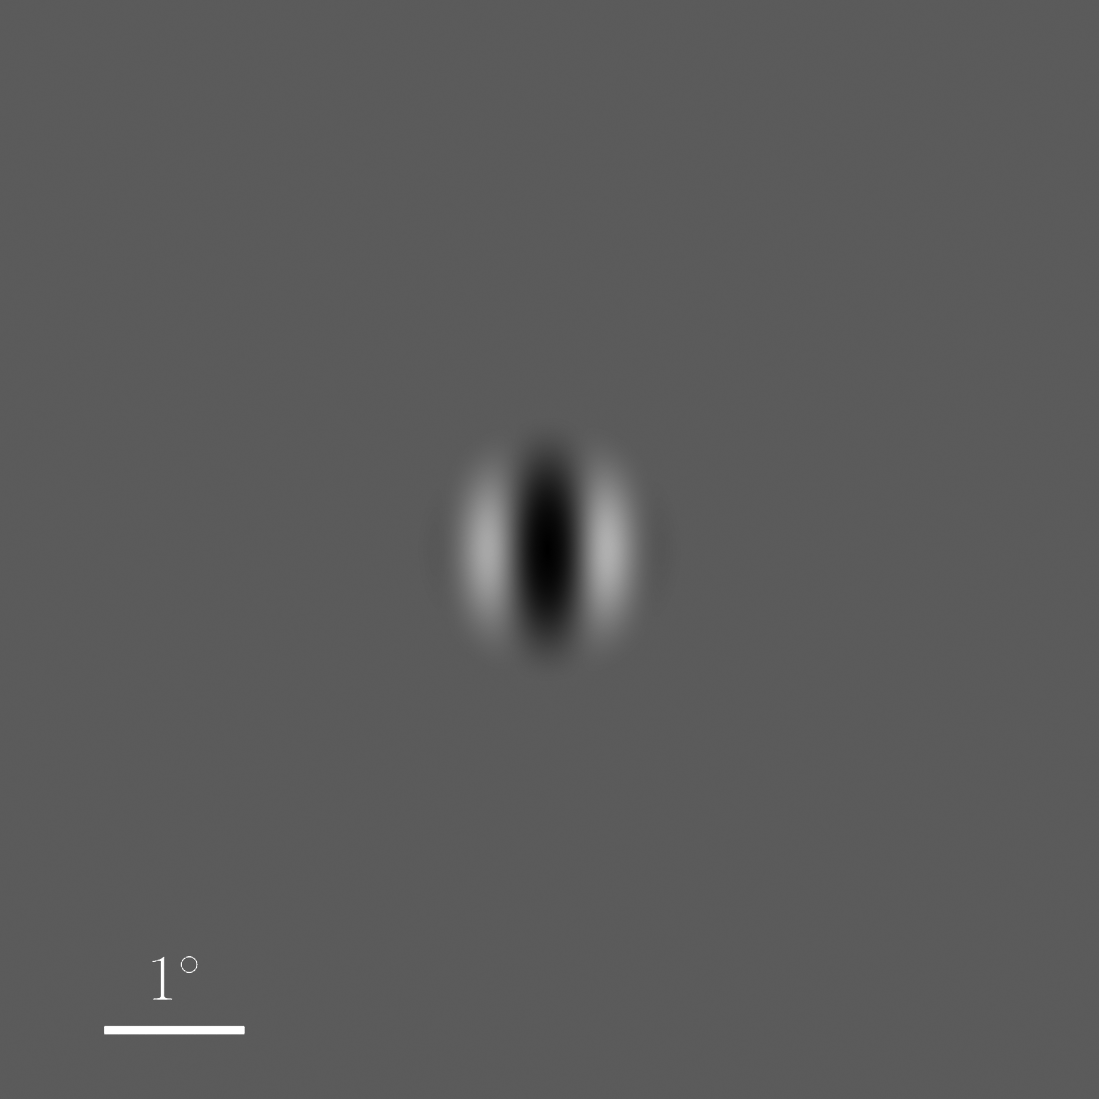
\includegraphics[width=0.48\textwidth]{png/s1_a}}~~
	\subfloat[Sehwinkel $= 3.6^{\circ}$][Sehwinkel $= 3.6^{\circ}$]{
\includegraphics[width=0.48\textwidth]{png/s2_a}}

	\subfloat[Sehwinkel $= 5.4^{\circ}$][Sehwinkel $= 5.4^{\circ}$]{
\includegraphics[width=0.48\textwidth]{png/s3_a}}~~
	\subfloat[Sehwinkel $= 7.2^{\circ}$][Sehwinkel $= 7.2^{\circ}$]{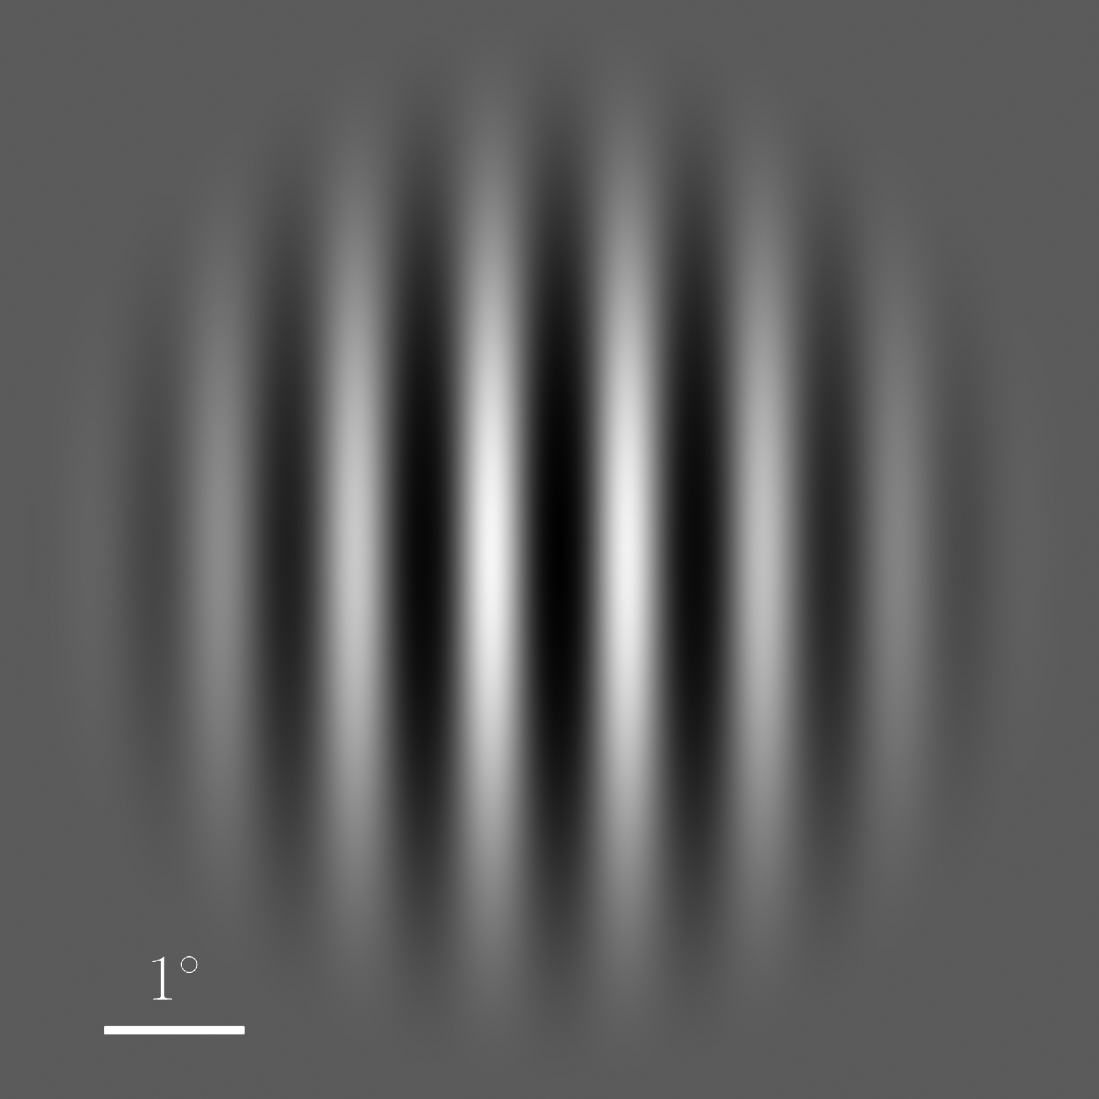
\includegraphics[width=0.48\textwidth]{png/s4_a}}

	\caption[Die Spatial-Suppression-Bedingungen]{Die vier Mustergrössen $(a - d)$ der \gls{ssauf}.}
	\label{fig:spatial_suppression_stimuli}
\end{figure}

\subsection{Versuchsablauf \label{subsec:Spatial-Suppression_Versuchsablauf}}

Ein Durchgang sah folgendermassen aus: Nach einer Zeitspanne von $440$~ms erschien in der Mitte des Monitors für $560$~ms ein Kreis, der sich über die ersten $200$~ms von einer Grösse von $1.6^{\circ}$ auf eine Grösse von $0.26^{\circ}$ zusammenzog, für $360$~ms diese Grösse beibehielt und anschliessend ausgeblendet wurde. Dieses Vorgehen diente dazu, den Blick der \glspl{vp} in die Bildschirmmitte zu lenken. Nach einem  Intervall von $300$~ms erschien in der Mitte des Monitors ein sich nach links oder rechts bewegendes vertikal schwarz-grau gestreiftes Musters. Die Stelle, an welcher die \glspl{vp} das Muster auf dem Monitor sahen, war stationär. Hinter dieser stationären Stelle bewegte sich das Muster mit einer Geschwindigkeit von $4^\circ / \textnormal{s} $  nach links oder nach rechts. Nach der Darbietungszeit mussten die \glspl{vp} mit einem Tastendruck entscheiden, in welche Richtung sich das Muster bewegt hat. Die \glspl{vp} erhielten die Instruktion, bei einer wahrgenommenen Bewegung nach links mit ihrem linken Zeigefinger die linke Pfeiltaste  und bei einer wahrgenommen Bewegung nach Rechts mit ihrem rechten Zeigefinger die rechte Pfeiltaste zu drücken. 
Bei einer korrekten Antwort wurde ein Ton abgegeben und die Darbietungszeit des nächsten Musters verringert, bei einer falschen Antwort wurde kein Ton abgegeben und die Darbietungszeit des nächsten Musters erhöht. 
Die Darbietungszeit des Musters wurde entsprechend dem QUEST-Ver\-fah\-ren \citep{Watson1983} angepasst.
Das QUEST-Ver\-fah\-ren ist adaptiv und arbeitet mit logarithmierten Werten, das heisst alle Berechnungen des Verfahrens finden im logarithmierten Raum statt. Der Algorithmus schätzt dabei mit Hilfe von Grundprinzipien der Bayes-Statistik nach jeder Antwort eine $\log_{10}$-Erkennungsschwelle für einen im Voraus bestimmten Prozentsatz an korrekten Antworten (in der hier vorliegenden Aufgabe betrug der Prozentsatz $82\,\%$).
Die geschätzte $\log_{10}$-Erkennungsschwelle wird dann vom Algorithmus benutzt, um die Darbietungszeit des nächsten Stimulus zu bestimmen. 
Die \glspl{vp} wurden instruiert, sich bei der Antwortabgabe genügend Zeit zu lassen und möglichst fehlerfrei zu arbeiten. Nach Antwortabgabe startete der nächste Durchgang.

Als Erstes bearbeiteten die \glspl{vp} eine Übungsaufgabe. Dabei wurden die vier Mustergrössen allen \glspl{vp} je drei Mal in einer pseudorandomisierten Abfolge präsentiert. Die Darbietungszeit aller Mustergrössen betrug zu Beginn der Aufgabe $80$~ms und wurde adaptiv angepasst. Die Übungsaufgabe dauerte etwa eine Minute und wurde nicht ausgewertet. Die $12$~Durchgänge der Übungsaufgabe dienten dazu, dass sich die \glspl{vp} mit der Art der Stimuluspräsentation, der Antworteingabe und dem Ton vertraut machen konnten. 

Als Zweites folgte eine etwas längere Aufgabe. Die \glspl{vp} bearbeiteten drei Wiederholungen, die durch eine Pause von etwa $30$~Sekunden getrennt waren. Eine Wiederholung bestand aus zwei Schätzungen der $82\,\%$-$\log_{10}$-Er\-ken\-nungs\-schwel\-le pro Mustergrösse. Jede der vier Mustergrössen wurde innerhalb einer Schätzung sieben Mal präsentiert. Gesamthaft bearbeiteten die \glspl{vp} folglich $3 \times 2 \times 4 \times 7 = 168$ Durchgänge. Die Mustergrössen wurde allen \glspl{vp} in einer pseudorandomisierten Abfolge präsentiert. Die Darbietungszeit der Mustergrössen betrug zu Beginn der Aufgabe $30$~ms und wurde für jede Mustergrösse einzeln über den gesamten Verlauf der $42$~Durchgänge adaptiv angepasst. Die Aufgabe dauerte etwa $7$~Minuten und wurde nicht ausgewertet, weil sich bei einigen \glspl{vp} die Wahrnehmungsleistung während der ersten Durchgänge stark verbessern kann (D. Tadin, persönl. Mitteilung, 19.08.2014). Dieser Aufgabenblock diente dazu, diese Trainingseffekte zuzulassen und die Leistung der \glspl{vp} auf ihrem individuellem Niveau zu festigen. 

Als Drittes wurde den \glspl{vp} die eigentliche Aufgabe vorgelegt. Die \glspl{vp} bearbeiteten drei Wiederholungen, die durch eine Pause von etwa einer Minute getrennt waren. Eine Wiederholung bestand aus zwei Schätzungen der $82\,\%$-$\log_{10}$-Er\-ken\-nungs\-schwel\-le pro Mustergrösse. Jede der vier Mustergrössen wurde innerhalb einer Schätzung $22$~Mal präsentiert. Gesamthaft bearbeiteten die \glspl{vp} somit $3 \times 2 \times 4 \times 22 = 528$ Durchgänge. 
Daraus resultierten für jede \gls{vp} 24 Schätzungen der $82\,\%$-$\log_{10}$-Er\-ken\-nungs\-schwel\-le (sechs pro Mustergrösse).
Die Mustergrössen wurde allen \glspl{vp} in einer pseudorandomisierten Abfolge präsentiert. Die Darbietungszeit der Mustergrössen betrug bei Start der Aufgabe $30$~ms und wurde für jede Mustergrösse einzeln über den gesamten Verlauf der $132$~Durchgänge adaptiv angepasst. 
Die Aufgabe dauerte etwa $25$~Minuten. 

Für jede \gls{vp} wurden die sechs pro Mustergrösse erhaltenen $82\,\%$-$\log_{10}$-Er\-ken\-nungs\-schwel\-len in eine Rangreihenfolge gebracht, die tiefste und höchste Schätzung entfernt und die restlichen vier $82\,\%$-$\log_{10}$-Er\-ken\-nungs\-schwel\-len gemittelt. Damit resultierte für jede \gls{vp} pro Mustergrösse ($1.8^{\circ}$, $3.6^{\circ}$, $5.4^{\circ}$ und $7.2^{\circ}$) eine $82\,\%$-$\log_{10}$-Er\-ken\-nungs\-schwel\-le für horizontale Bewegung. 
Alle Berechnungen wurden mit diesen $82\,\%$-$\log_{10}$-Er\-ken\-nungs\-schwel\-len getätigt. 
Ausnahme bildete die exponentielle Regression (siehe \autoref{sec:2Fragestellung}), bei welcher die vier $82\,\%$-$\log_{10}$-Er\-ken\-nungs\-schwel\-len auf Anraten von D. Tadin (persönl. Mitteilung, 11.02.2016) als Exponenten zur Basis 10 verrechnet und in dieser invertierten Form analysiert wurden.
Um die Interpretation der logarithmierten Werte zu erleichtern, wurden sie für die Ergebnisdarstellung (in Tabellen und Abbildungen) invertiert.
Der \gls{si} wurde gemäss der Vorgehensweise von \citet{Melnick2013} als Differenz zwischen der $82\,\%$-$\log_{10}$-Er\-ken\-nungs\-schwel\-le für die Mustergrösse $7.2^{\circ}$ und der $82\,\%$-$\log_{10}$-Er\-ken\-nungs\-schwel\-le für die Mustergrösse $1.8^{\circ}$ gebildet. 


\section{Die Hick-Aufgabe \label{sec:Hick}}

Angelehnt an die Versuchsanordnung von \citet{Rammsayer2007} wurde als Mass für \gls{ms} eine \gls{ha} eingesetzt.

\subsection{Apparatur und Material \label{sub:}}
Präsentiert wurde die Aufgabe auf dem in \autoref{sub:ssas} beschriebenen Computer, mit dem einzigen Unterschied, dass die Auflösung des Monitors für die \gls{ha} $1280 \times 1024$ Pixel betrug. Die Antworten der \glspl{vp} wurden mit einer Cedrus RB-830 Tastatur erfasst. 

Die Stimuli wurden mit E-Prime\textsuperscript{\textregistered} \citep{eprime} generiert. Die weissen Stimuli wurden auf einem schwarzen Hintergrund präsentiert, welcher eine Leuchtdichte von $2\,\textnormal{cd}/ \textnormal{m}^2$ aufwies. Der horizontale und vertikale Sehwinkel der verwendeten Rechtecke betrug $1.8^{\circ}$ respektive $1.5^{\circ}$. Die Rechtecke wurden auf dem Monitor zentriert dargeboten. Die Stimulianordnung der verwendeten Bedingungen sah folgendermassen aus (siehe \autoref{fig:hick_stimuli}):  In der $0$-Bit-Bedingung wurde ein Rechteck präsentiert. In der $1$-Bit-Bedingung wurden horizontal nebeneinander zwei Rechtecke präsentiert. Die beiden Rechtecke erschlossen zusammen einen horizontalen und vertikalen Sehwinkel von $4.5^{\circ}$ respektive $1.5^{\circ}$. In der $2$-Bit-Bedingung wurden in U-Form vier Rechtecke präsentiert. Die vier Rechtecke erschlossen gemeinsam einen horizontalen und vertikalen Sehwinkel von $7.5^{\circ}$ respektive $4.3^{\circ}$. In der $2.58$-Bit-Bedingung wurden zu den in U-Form angeordneten vier Rechtecken der $2$-Bit-Bedingung in der oberen Reihe je links und rechts ein Rechteck hinzugefügt. Die sechs Rechtecke erschlossen zusammen einen horizontalen und vertikalen Sehwinkel von $12.9^{\circ}$ respektive $4.3^{\circ}$. Der Sehwinkel des imperativen Reizes, einem \enquote{+}, betrug $0.5^{\circ}$ und wurde  immer in der Mitte eines Rechtecks präsentiert. Die Sehwinkel der Stimuli wurden mit einer Kinnstütze, die $61$ cm vom Monitor entfernt war, sichergestellt. Der verwendete Ton wies bei einer Frequenz von $1000$~Hz und einer Lautstärke von $70$~dB eine Länge von $200$~ms auf.

\begin{figure}[htbp]
	\centering
	\subfloat[0-Bit]		[0-Bit-Bedingung]	{
		\resizebox{.9\textwidth}{!}{
			\begin{tikzpicture}
			[scale=1, font=\sffamily, inner sep=0pt, baseline,
			manifest/.style		= {draw, rectangle, thick, white, inner sep=0pt, minimum width=19mm, minimum height=16mm},
			invisible/.style	= {draw, rectangle, thick, black!80, inner sep=0pt, minimum width=19mm, minimum height=16mm},
			visual/.style 		= {draw, rectangle, thick, white, fill=white!100, minimum width= 10.65mm, minimum height=.5mm}]
			
			\node [invisible]	at (0,0)							(3)	{};
			\node [invisible]	[right = 11mm of 3]	  				(4)	{};
			\node [invisible]	[above left  = 15mm and -3mm of 3]	(2) {};
			\node [invisible]	[above right = 15mm and -3mm of 4]	(5) {};
			\node [invisible]	[left  = 11mm of 2]	  				(1)	{};
			\node [invisible]	[right = 11mm of 5]	  				(6)	{};
			
			\node [manifest] at (1.5,1.5)							(9)	{\Huge $+$};
			
			\node [visual]		at (-5,-1)	{}							;
			\node [white]		at (-5,-.6) {\Large$1^{\circ}$}		;
			
			\begin{scope}[on background layer]
				\node [fill=black!80, inner sep= 20pt, fit=(1) (2) (3) (4) (5) (6)] {};
			\end{scope}
			\end{tikzpicture}
}} \newline

\subfloat[1-Bit]		[1-Bit-Bedingung]	{
	\resizebox{.9\textwidth}{!}{
		\begin{tikzpicture}
		[scale=1, font=\sffamily, inner sep=0pt,
		manifest/.style		= {draw, rectangle, thick, white, inner sep=0pt, minimum width=19mm, minimum height=16mm},
		invisible/.style	= {draw, rectangle, thick, black!80, inner sep=0pt, minimum width=19mm, minimum height=16mm},
		visual/.style 		= {draw, rectangle, thick, white, fill=white!100, minimum width= 10.65mm, minimum height=.5mm}]
		
		\node [invisible]	at (0,0)							(3)	{};
		\node [invisible]	[right = 11mm of 3]	  				(4)	{};
		\node [invisible]	[above left  = 15mm and -3mm of 3]	(2) {};
		\node [invisible]	[above right = 15mm and -3mm of 4]	(5) {};
		\node [invisible]	[left  = 11mm of 2]	  				(1)	{};
		\node [invisible]	[right = 11mm of 5]	  				(6)	{};
		
		\node [manifest] at (0,1.5)				(9)		{\Huge $+$}	;
		\node [manifest] [right = 11mm of 9] 	(10)	{}			;	
		
		\node [visual]		at (-5,-1)	{}							;
		\node [white]		at (-5,-.6) {\Large$1^{\circ}$}		;
		
		\begin{scope}[on background layer]
		\node [fill=black!80, inner sep= 20pt, fit=(1) (2) (3) (4) (5) (6)] {};
		\end{scope}
		\end{tikzpicture}
	}} \newline
	
	\subfloat[2-Bit]		[2-Bit-Bedingung]	{
		\resizebox{.9\textwidth}{!}{
			\begin{tikzpicture}
			[scale=1, font=\sffamily, inner sep=0pt,
			manifest/.style		= {draw, rectangle, thick, white, inner sep=0pt, minimum width=19mm, minimum height=16mm},
			invisible/.style	= {draw, rectangle, thick, black!80, inner sep=0pt, minimum width=19mm, minimum height=16mm},
			visual/.style 		= {draw, rectangle, thick, white, fill=white!100, minimum width= 10.65mm, minimum height=.5mm}]
			
			\node [invisible]	at (0,0)							(3)	{};
			\node [invisible]	[right = 11mm of 3]	  				(4)	{};
			\node [invisible]	[above left  = 15mm and -3mm of 3]	(2) {};
			\node [invisible]	[above right = 15mm and -3mm of 4]	(5) {};
			\node [invisible]	[left  = 11mm of 2]	  				(1)	{};
			\node [invisible]	[right = 11mm of 5]	  				(6)	{};
			
			\node [manifest]	at (0,0)							(3)	{};
			\node [manifest]	[right = 11mm of 3]	  				(4)	{};
			\node [manifest]	[above left  = 15mm and -3mm of 3]	(2) {\Huge $+$};
			\node [manifest]	[above right = 15mm and -3mm of 4]	(5) {};	
			
			\node [visual]		at (-5,-1)	{}							;
			\node [white]		at (-5,-.6) {\Large$1^{\circ}$}		;
			
			\begin{scope}[on background layer]
			\node [fill=black!80, inner sep= 20pt, fit=(1) (2) (3) (4) (5) (6)] {};
			\end{scope}
			\end{tikzpicture}
		}} \newline
		
		\subfloat[$2.58$-Bit]		[$2.58$-Bit-Bedingung]	{
			\resizebox{.9\textwidth}{!}{
				\begin{tikzpicture}
				[scale=1, font=\sffamily, inner sep=0pt,
				manifest/.style		= {draw, rectangle, thick, white, inner sep=0pt, minimum width=19mm, minimum height=16mm},
				invisible/.style	= {draw, rectangle, thick, black!80, inner sep=0pt, minimum width=19mm, minimum height=16mm},
				visual/.style 		= {draw, rectangle, thick, white, fill=white!100, minimum width= 10.65mm, minimum height=.5mm}]
				
				\node [invisible]	at (0,0)							(3)	{};
				\node [invisible]	[right = 11mm of 3]	  				(4)	{};
				\node [invisible]	[above left  = 15mm and -3mm of 3]	(2) {};
				\node [invisible]	[above right = 15mm and -3mm of 4]	(5) {};
				\node [invisible]	[left  = 11mm of 2]	  				(1)	{};
				\node [invisible]	[right = 11mm of 5]	  				(6)	{};
				
				\node [manifest]	at (0,0)							(3)	{};
				\node [manifest]	[right = 11mm of 3]	  				(4)	{};
				\node [manifest]	[above left  = 15mm and -3mm of 3]	(2) {};
				\node [manifest]	[above right = 15mm and -3mm of 4]	(5) {};
				\node [manifest]	[left  = 11mm of 2]	  				(1)	{};
				\node [manifest]	[right = 11mm of 5]	  				(6)	{\Huge $+$};
				
				\node [visual]		at (-5,-1)	{}							;
				\node [white]		at (-5,-.6) {\Large$1^{\circ}$}		;
				
				\begin{scope}[on background layer]
				\node [fill=black!80, inner sep= 20pt, fit=(1) (2) (3) (4) (5) (6)] {};
				\end{scope}
				\end{tikzpicture}
			}} \newline
			
			\caption[Die Hick-Bedingungen]{Die vier Bedingungen $(a - d)$ der \gls{ha}. }
			\label{fig:hick_stimuli}
\end{figure}




\subsection{Versuchsablauf \label{subsec:hick_Versuchsablauf}}

In der $0$-Bit-Bedingung bearbeiteten die \glspl{vp} $32$ Durchgänge. Jeder Durchgang startete nach $1100$ ms mit der Präsentation eines Rechtecks. Nach einer variablen Zeitdauer, \gls{soa} genannt, welche $1000$, $1333$, $1666$ oder $2000$ ms betrug, wurde der imperative Reiz, ein \enquote{+}, eingeblendet. Die \glspl{vp} wurden angewiesen, mit dem Zeigefinger ihrer dominanten Hand so rasch als möglich auf die vorgesehene Antworttaste zu drücken. Bei einer Antwortabgabe nach Einblenden des imperativen Reizes folgte ein Ton. Bei einer Antwortabgabe vor Einblenden des imperativen Reizes folgte kein Ton. In beiden Fällen führte eine Antwortabgabe zur Ausblendung der Stimuli und zum Start des nächsten Durchganges.

Die $1$-Bit-Bedingung unterschied sich von der $0$-Bit-Bedingung in der Anzahl dargebotener Rechtecke und der Tonabgabe. Der imperative Reiz trat im linken oder im rechten Rechteck auf. Die \glspl{vp} erhielten die Anweisung, beim Auftreten des imperativen Reizes im linken Rechteck mit ihrem linken Zeigefinger und beim Auftreten des imperativen Reizes im rechten Rechteck mit ihrem rechten Zeigefinger so rasch als möglich auf die dem jeweiligen Finger zugewiesene Antworttaste zu drücken. Bei einer korrekten Antwortabgabe nach Einblendung des imperativen Reizes folgte ein Ton. Bei einer Antwortabgabe vor Einblendung des imperativen Reizes oder bei einer falschen Antwortabgabe folgte kein Ton.

Die $2$-Bit-Bedingung unterschied sich von der $1$-Bit-Bedingung lediglich in der Anzahl präsentierter Rechtecke. Der imperative Reiz trat entweder im oberen linken, unteren linken, oberen rechten oder unteren rechten Rechteck auf. Die \glspl{vp} wurden angewiesen, beim Auftreten des imperativen Reizes im oberen linken Rechteck mit ihrem linken Mittelfinger, beim Auftreten des imperativen Reizes im unteren linken Rechteck mit ihrem linken Zeigefinger,  beim Auftreten des imperativen Reizes im oberen rechten Rechteck mit ihrem rechten Mittelfinger und beim Auftreten des imperativen Reizes im unteren rechten Rechteck mit ihrem rechten Zeigefinger so rasch als möglich auf die dem jeweiligen Finger zugewiesene Antworttaste zu drücken.

Die $2.58$-Bit-Bedingung unterschied sich von der $2$-Bit-Bedingung nur in der Anzahl präsentierter Rechtecke. Der imperative Reiz trat entweder im oberen äusseren linken, oberen inneren linken, unteren linken, oberen äusseren rechten, oberen inneren rechten oder unteren rechten Rechteck auf. Die \glspl{vp} wurden angewiesen, beim Auftreten des imperativen Reizes im oberen äusseren linken Rechteck mit ihrem linken Ringfinger, beim Auftreten des imperativen Reizes im oberen inneren linken Rechteck mit ihrem linken Mittelfinger, beim Auftreten des imperativen Reizes im unteren linken Rechteck mit ihrem linken Zeigefinger, beim Auftreten des imperativen Reizes im oberen äusseren Rechteck mit ihrem rechten Ringfinger, beim Auftreten des imperativen Reizes oberen inneren rechten Rechteck mit ihrem rechten Mittelfinger und beim Auftreten des imperativen Reizes im unteren rechten Rechteck mit ihrem rechten Zeigefinger so rasch als möglich auf die dem jeweiligen Finger zugewiesene Antworttaste zu drücken.

Die Bedingungen wurden von allen \glspl{vp} in aufsteigender Reihenfolge ($0$-, $1$-, $2$-, $2.58$-Bit-Bedingung) bearbeitet. Jeder Bedingung gingen acht  Übungsdurchgänge voraus, damit sich die \glspl{vp} mit der Art der Stimuluspräsentation, der Antworteingabe und dem Ton vertraut machen konnten. 
Der imperative Reiz trat in der $1$-, $2$- und $2.58$-Bit-Bedingung für alle \glspl{vp} in einer pseudorandomisierten Abfolge mit der identischen, ausbalancierten \gls{soa} am identischen, über die $32$~Durchgänge der Bedingungen ausbalancierten Ort auf. Insgesamt dauerte die Aufgabe etwa $15$~Minuten. 

Pro Bedingung wurde für jede \gls{vp} der Mittelwert und die Standardabweichung aller korrekten Antworten bestimmt, die zwischen $100$ und $2500$~ms lagen. Basierend auf diesen Berechnungen wurden für jede \gls{vp} in jeder Bedingung diejenigen Durchgänge entfernt, welche eine \gls{rz} $\geq$ \gls{m} $+\,3\,\times$ \gls{sd} aufwiesen. Nach dieser intraindividuellen Ausreisserkontrolle wurden die verbliebenen Durchgänge innerhalb einer Bedingung gemittelt und für jede \gls{vp} als Leistungsmass der Bedingung der \gls{ha} verwendet.


\section{Erfassung der psychometrischen Intelligenz \label{sec:Erfassung_der_psychometrischen_Intelligenz}}

\glsunset{bist} % see http://tex.stackexchange.com/questions/30167/suppress-the-glossary-expansion-at-first-occurance
\glsunset{bism}

Psychometrische Intelligenz wurde mit einer modifizierten Kurzversion des \acrlong{bist}s \citep[\gls{bist};][]{Jaeger1997} erfasst. Die fähigkeitstheoretische Grundlage des Tests ist das integrativ konzipierte bimodale und hierarchische \acrlong{bism} (\gls{bism}; siehe \autoref{fig:bis_model}) von \citet{Jaeger1984}.

\begin{figure}[b]
	\centering
	\begin{adjustbox}{width=.9\textwidth}
		\begin{tikzpicture}
		[scale=1, font=\sffamily, inner sep=0pt]
		
		\draw[dashed]	(0, 0) -- (4, 6) -- (7, 1.5) -- (3, -4.5) -- (0, 0);
		
		\draw[dashed]	(1, 1.5) -- (4, -3);
		\draw[dashed]	(2, 3) -- (5, -1.5);
		\draw[dashed]	(3, 4.5) -- (6, 0);
		
		\draw[dashed]	(1, -1.5) -- (5, 4.5);
		\draw[dashed]	(2, -3) -- (6, 3);
		
		\draw			(0, 6.6) -- (1, 7) -- (6, 7) -- (7, 6.6);
		
%		\draw[draw=none] (1, 7.1) -- (6, 7.1)
%		node[pos=0.5, rotate=0, above=1]{\LARGE AI - {\textrm{\textit{g}}}\textsubscript{\tiny BIS}};
		
		\draw[draw=none] (1, 7.1) -- (6, 7.1)
		node[pos=0.5, rotate=0, above=.2]{\Large Allgemeine Intelligenz (AI)};
		
		\draw[draw=none] (0, 0) -- (4, 6)
		node[pos=0.4, rotate=56, above=1]{\LARGE{OPERATIONEN}};
		
		\draw[draw=none] (4, 6) -- (7, 1.5)
		node[pos=0.63, rotate=-56, above=1]{\LARGE{INHALTE}};
		
		
		% F content ----------------------------------------------
		\draw[draw=none] (0, -1)
		node {\LARGE{F}};
		
		\draw[draw=none] (-1, -1)
		node[above=.05]{\scriptsize Figural-}
		node[below=.05]{\scriptsize bildhaft};
		
		% V content ----------------------------------------------
		\draw[draw=none] (1, -2.5)
		node{\LARGE{V}};
		
		\draw[draw=none] (0.1, -2.5)
		node{\scriptsize Verbal};
		
		% N content ----------------------------------------------
		\draw[draw=none] (2, -4)
		node{\LARGE{N}};
		
		\draw[draw=none] (.8, -4)
		node{\scriptsize Numerisch};
		
		% B operation --------------------------------------------
		\draw[draw=none] (7, 0.5)
		node {\LARGE{B}};
		
		\draw[draw=none] (8.5, 0.5)
		node[above=.05]{\scriptsize Bearbeitungs-\hphantom{iit}}
		node[below=.05]{\scriptsize geschwindigkeit};
		
		% M operation --------------------------------------------
		\draw[draw=none] (6, -1)
		node {\LARGE{M}};
		
		\draw[draw=none] (7.5, -1)
		node{\scriptsize Merkfähigkeit};
		
		% E operation --------------------------------------------
		\draw[draw=none] (5, -2.5)
		node {\LARGE{E}};
		
		\draw[draw=none] (6.5, -2.5)
		node{\scriptsize Einfallsreichtum};
		
		% K operation --------------------------------------------
		\draw[draw=none] (4, -4)
		node {\LARGE{K}};
		
		\draw[draw=none] (5.9, -4)
		node{\scriptsize Verarbeitungskapazität};
		\end{tikzpicture}
	\end{adjustbox}
	\vspace*{.5cm}
	\caption[Das Berliner Intelligenzstrukturmodell]{Das Berliner Intelligenzstrukturmodell von \citet{Jaeger1984}.}
	\label{fig:bis_model}
\end{figure}

Als integratives Modell ist das \gls{bism} zu bezeichnen, weil \citet{Jaeger1984} bei der Konstruktion des Modells versucht hat, die Vielfalt intellektueller Leistungsformen möglichst umfassend zu repräsentieren.
Bimodal ist das \gls{bism}, weil das Modell zwei Modalitäten aufweist, unter welchen Leistungen und Fähigkeiten klassifiziert werden können. 
Das \gls{bism} trennt dabei zwischen sogenannten Operationen und Inhalten. Innerhalb der Modalität Operationen werden die vier Fähigkeitsbündel Verarbeitungskapazität, Bearbeitungsgeschwindigkeit, Merkfähigkeit und Einfallsreichtum unterschieden. 
\gls{k} steht für die Fähigkeit, komplexe Informationen von Aufgaben zu verarbeiten, die nicht auf Anhieb zu lösen sind, sondern die erst durch vielfältiges Beziehungsstiften, formallogisch exaktes Denken und sachgerechtes Beurteilen von Informationen zu lösen sind. 
\gls{b} beschreibt das Arbeitstempo, die Auffassungsleichtigkeit und die Konzentrationskraft beim Lösen von einfach strukturierten Aufgaben mit geringem Schwierigkeitsgrad. 
\gls{M} spiegelt die Fähigkeit wider, sich etwas aktiv einzuprägen, etwas kurzfristig wieder zu erkennen oder zu reproduzieren. 
\gls{e} beschreibt die Fähigkeit, flexible Ideen zu produzieren und über vielfältige Vorstellungen von Problemen zu verfügen. 
Innerhalb der Modalität Inhalte lässt sich nach \citet{Jaeger1984} sprachgebundenes Denken von zahlengebundenem Denken und anschauungsgebundenem, figural-bildhaftem Denken unterscheiden.
\Gls{v} beschreibt den Grad der Aneignung und der Verfügbarkeit des Beziehungssystems Sprache.
\Gls{n} steht für das Ausmass der Aneignung und der Verfügbarkeit des Beziehungssystems Zahlen.
\Gls{f} spiegelt die Fähigkeit wider, Aufgabenmaterial zu verarbeiten, welches bildhaftes beziehungsweise räumliches Vorstellen erfordert.

Auf höchster Hierarchiestufe des \gls{bism} steht als Integral aller sieben Fähigkeiten (\gls{k}, \gls{b}, \gls{M}, \gls{e}, \gls{v}, \gls{n} und \gls{f}) die \gls{ai}. Die \gls{ai} und die Fähigkeiten unterscheiden sich aber lediglich im Differenzierungsgrad. \gls{ai} bildet Intelligenzleistungen gemäss \citet{Jaeger1984} aus grosser Distanz ab, während die sieben Fähigkeiten auf der Ebene darunter Intelligenzleistungen aus geringerer Distanz mit feinerem Auflösungsgrad abbilden. Untersuchungen zum \gls{bism} konnten die postulierte Struktur des \gls{bist}s replizieren  und Zusammenhänge mit anderen Intelligenzmodellen wie denjenigen von \citet{Cattell1971}  oder von \citet{Carroll1993} herstellen \citep{Bucik1996, Beauducel2002, Suess2002}.

Die von \citet{Jaeger1997} vorgeschlagene Kurzversion des \gls{bist}s enthält $15$ Subtests. Die Operationen \gls{b}, \gls{M} und \gls{e} werden darin mit je einem Subtest pro Inhalt erfasst, wobei \gls{k} mit zwei Subtests pro Inhalt erfasst wird. Bei der Modellierung der Daten mittels Strukturgleichungsmodellen hätte dies bei der vorliegenden Arbeit zu einer Überrepräsentation von \gls{k} im \gls{gfaktor} geführt. Um dies zu vermeiden, wurden die Operationen \gls{b} und \gls{M} um je einen Subtest pro Inhalt angereichert. Grundlage für die Auswahl der Subtests bildeten die Erkenntnisse von \citet{Wicki2014}, wobei bei der Entscheidung über die Aufnahme der Subtests ökonomische (Bearbeitungszeit der Subtests) und teststatistische (Trennschärfe und Reliabilität der Subtests)  Gesichtspunkte berücksichtigt wurden. Die Kurzversion von \citet{Jaeger1997} wurde mit folgenden Subtests ergänzt: Klassifizieren von Wörtern, Old English, Rechen-Zeichen, Wege-Erinnern, Worte Merken und Zweistellige Zahlen. 
\citet{Wicki2014} berichtet für diese modifizierte Kurzversion für die Operationen \gls{k}, \gls{b} und \gls{M} interne Konsistenzen von Cronbachs $\alpha=.61-.73$ und Konstruktreliabilitäten, gemessen mit \citeauthor{McDonald1999}\textcolor{blue}{s} \citeyearpar{McDonald1999} Omegakoeffizienten, von $\Omega = .58-.64$.
Auf Subtests der Operation \gls{e} wurde gänzlich verzichtet, weil zum einen unklar ist, wie Einfallsreichtum und Intelligenz zusammenhängen \citep{Kim2005} und zum anderen weil \citet{Jaeger1997} unbefriedigende Objektivitätswerte berichten. 
Alle eingesetzten Subtests, deren Beschreibung sowie Zuordnung zu den jeweiligen Operationen und Inhalte sind \autoref{tab:bis_subtest_description} zu entnehmen.




\begin{sidewaystable}
	\captionsetup{labelsep = none}
	\caption[Die verwendeten Subtests des \gls{bist}s]{\newline  \textit{Beschreibung und Reihenfolge der eingesetzten Subtests des \gls{bist}s} \vspace{.2cm}}
	\label{tab:bis_subtest_description}
	\begin{adjustbox}{width=\textwidth,totalheight=.9\textheight,keepaspectratio}
		\begin{threeparttable}
			\begin{tabular}{l l c c c c p{.0001cm} c c c p{20cm}}
				\hline
					&		&		& \multicolumn{3}{c}{Operation}	&	&	\multicolumn{3}{c}{Inhalt}	&		\\
				\cline{4-6}
				\cline{8-10}
				\multicolumn{1}{c}{Nr.}	&	\multicolumn{1}{c}{Name}	&	\multicolumn{1}{c}{Abkürzung}	&		K	&	B	&	M		&	&		V	&	N	&	F		&	\multicolumn{1}{c}{Beschreibung}	\\
				
				\hline
				1				&	Unvollständige Wörter*	&	UW			&&	\checkmark	&&&\checkmark&&& In vorgegebenen Wörtern fehlen einige Buchstaben, welche zu ergänzen sind (z. B. F\_scher)	\\
				2				&	Orientierungs-Gedächtnis	&	OG		&&&	\checkmark	&&&&\checkmark& Auf einem Stadtplanausschnitt markierte Gebäude müssen eingeprägt und unmittelbar danach wiedergegeben werden\\
				3				&	Zahlenreihen			&	ZN			&	\checkmark	&&&&&\checkmark&& Nach bestimmten Regeln aufgebaute Zahlenreihen sind um ein weiteres Glied zu ergänzen (z. B. 2 5 8 11 14 17 ?)\\
				4				&	Analogien				&	AN			&	\checkmark	&&&&&&\checkmark& Analogien mit Form $A:B=C:\,?$ müssen ergänzt werden, wobei die Analogien aus geometrischen Formen bestehen\\
				5				&	X-Grösser				&	XG			&&	\checkmark	&&&&\checkmark&& Zahlen, die um $3$ grösser sind als die unmittelbar vorangegangene Zahl müssen so schnell wie möglich durchgestrichen werden (z. B. 18 20 24 \cancel{27} 13 18 \cancel{21} \ldots)\\
				6				&	Wortanalogien			&	WA			&	\checkmark	&&&&\checkmark&&& Wortanalogien der Form \enquote{Huhn zu Küken} wie \enquote{Kuh zu ?} müssen vervollständigt werden\\
				7				&	Zahlenpaare				&	ZP			&&&	\checkmark	&&&\checkmark&& Zahlenpaare der Form 71 -- 918 sind einzuprägen. Das jeweils zweite Glied ist anschliessend unter vier Distraktoren zu identifizieren\\
				8				&	Tatsache-Meinung		&	TM			&	\checkmark	&&&&\checkmark&&& Sätze müssen daraufhin geprüft werden, ob sie eher eine Tatsache oder eher eine Meinung wiedergeben\\
				9				&	Buchstaben-Durchstreichen&	BD			&&	\checkmark	&&&&&\checkmark& Alle \enquote{x} müssen in Zeilen von Buchstaben durchgestrichen werden (z. B. sys\cancel{x}kdihj\cancel{x}\ldots)\\
				10				&	Schätzen				&	SC			&	\checkmark	&&&&&\checkmark&& Rechenaufgaben der Form $118492-3684-2106-4768=\,?$ müssen durch einfache rechnerische Überlegungen geschätzt bzw. gelöst werden\\
				11				&	Sinnvoller Text			&	ST			&&&	\checkmark	&&\checkmark&&& Verbale Detailangaben in einem Text sind einzuprägen und unmittelbar danach zu reproduzieren\\
				12				&	Charkow					&	CH			&	\checkmark	&&&&&&\checkmark& Eine Folge von Strichzeichnungen, die nach einer bestimmten Regel aufgebaut ist, ist um die beiden folgenden Glieder zu ergänzen\\
				13				&	Teil-Ganzes				&	TG			&&	\checkmark	&&&\checkmark&&& In Wortlisten sind zwei aufeinander folgende Wörter, die in der Beziehung Ganzes/zugehöriger Teil zueinander stehen zu markieren (z. B. Baum, \cancel{Blatt}, Stein, Haus, \cancel{Dach}, \ldots)\\
				14				&	Rechen--Zeichen			&	RZ			&&	\checkmark	&&&&\checkmark&& In  einfachen vorgegebenen Gleichungen stehen anstelle von Plus- oder Minuszeichen leere Kästchen. Die richtigen Rechenzeichen sind einzutragen\\
				15				&	Worte merken			&	WM			&&&	\checkmark	&&\checkmark&&& Eine Liste von Wörtern ist einzuprägen und unmittelbar danach in beliebiger Reihenfolge zu reproduzieren\\ 
				16				&	Klassifizieren von Wörtern&	KW			&&	\checkmark	&&&\checkmark&&& In Spalten von Wörtern sind alle Worte, die Pflanzen bezeichnen, durchzustreichen\\
				17				&	Zweistellige Zahlen		&	ZZ			&&&	\checkmark	&&&\checkmark&& Eine Reihe zweistelliger Zahlen ist einzuprägen und unmittelbar danach in beliebiger Reihenfolge zu reproduzieren\\
				18				&	Old English				&	OE			&&	\checkmark	&&&&&\checkmark& In Buchstabenreihen sind alle in einem vorgegebenen Schrifttyp gedruckten Buchstaben durchzustreichen\\
				19				&	Wege--Erinnern			&	WE			&&&	\checkmark	&&&&\checkmark& Ein in einem Stadtplanausschnitt eingezeichneter Weg ist einzuprägen und unmittelbar danach zu reproduzieren\\
				
				\hline
			\end{tabular}
			
			\begin{tablenotes}[flushleft]
				\footnotesize				% font size
				\setlength\labelsep{0pt}	% no indent on second line
				\item \textit{Anmerkungen.} K~=~Verarbeitungskapazität; B~=~Bearbeitungsgeschwindigkeit; M~=~Merkfähigkeit; V~=~verbal; N~=~numerisch; F~=~figural-bildhaft.\\
				{$^*$}Der Subtest UW wurde als Aufwärmaufgabe verwendet und floss nicht in die Auswertung mit ein.
			\end{tablenotes}
		\end{threeparttable}
	\end{adjustbox}
\end{sidewaystable}

Die $19$ Subtests wurden den \glspl{vp} nach der in \autoref{tab:bis_subtest_description} aufgeführten Reihenfolge vorgelegt und gemäss dem Manual des \gls{bist}s instruiert. 
Die Bearbeitung der Subtests dauerte insgesamt $50$ Minuten.
Die Aufwärmaufgabe \gls{uw} wurde nicht ausgewertet. Die Rohwerte der restlichen $18$~Subtests wurden \textit{z}-standardisiert. 
Für die Beantwortung der Fragestellungen 1 und 2 wurden alle $18$~\textit{z}-stand\-ard\-isier\-ten Subtests gemittelt. Dadurch resultierte für jede \glspl{vp} ein \textit{z}-standardisiertes Mittel ihrer Leistung. 
Um für die Beantwortung der Fragestellungen 3, 4 und 5 einen \gls{gfaktor} zu bilden, wurden die $18$~\textit{z}-standardisierten Subtests innerhalb ihrer zugehörigen Operation gemittelt. Damit flossen in jede Operation (\gls{k}, \gls{b} und \gls{M}) zwei Subtests aus dem Bereich \gls{v}, zwei Subtests aus dem Bereich \gls{n} und zwei Subtests aus dem Bereich \gls{f} (insgesamt sechs Subtests) ein. Der \gls{gfaktor} wurde anschliessend aus den drei gemittelten \textit{z}-Werten der Operationen \gls{k}, \gls{b} und \gls{M} abgeleitet.


\section{Weitere Instrumente}

Im Rahmen der Untersuchung wurden den \glspl{vp} Fragebögen und weitere Com\-put\-er-Auf\-gaben zur Bearbeitung vorgelegt. Sie sind für die Fragestellungen dieser Arbeit nicht relevant und werden deshalb im folgenden Abschnitt nur kurz beschrieben.


\subsection{Fragebögen}

\subsubsection*{Persönliche Angaben}
Die Erfassung persönlicher Angaben fand in zwei Teilen statt. In einem ersten Teil machten die \glspl{vp} schriftlich Angaben zu ihrer Muttersprache, Seh- und Hörfähigkeit, ihren chronischen Krankheiten und ihrem Medikamenten- sowie Nikotinkonsum. In einem zweiten Teil machten sie computergestützt Angaben zu ihrem Alter, Geschlecht, Bildungsniveau, Koffeinkonsum,  Videospielhäufigkeit, Musikinstrumenterfahrung und Vertrautheit mit dem Zehnfingersystem beim Computerschreiben.


\subsubsection*{Kurzform der deutschen Übersetzung des revidierten \gls{epq-rk}}
Die \glspl{vp} haben  computergestützt die Kurzform der deutschen Übersetzung des \gls{epq-rk} von \citet{Ruch1999} bearbeitet. Der Fragebogen enthält insgesamt $50$~Fragen, darunter $14$~Items zur Erfassung von Psychotizismus, $12$~Items zur Erfassung von Extraversion, $12$~Items zur Erfassung von Neurotizismus und $12$~Items zur Erfassung der individuellen Neigung, sozial erwünschte Antworten abzugben.

\subsubsection*{Deutsche Übersetzung des \gls{dii}}
Die deutsche Übersetzung des \gls{dii} stammt von \citet{Kuhmann1996} und beinhaltet insgesamt $23$~Items, darunter $11$~Items zur Erfassung der funktionalen Impulsivität und  $12$~Items zur Erfassung der dysfunktionalen Impulsivität. Der Fragebogen wurde von den \glspl{vp} computergestützt bearbeitet.

\subsection{Zeitverarbeitungsaufgaben}


\subsubsection*{Zeitdauerdiskrimination im Millisekundenbereich mit gefüllten und leeren Intervallen}

Angelehnt an die Versuchsanordnung von \citet{Stauffer2011} bekamen die \glspl{vp} über Lautsprecher hintereinander eine Standardtondauer und eine variable Vergleichstondauer dargeboten. Danach mussten die \glspl{vp} jeweils mit einem Tastendruck entscheiden, ob die erste oder die zweite Tondauer länger war. Bei einer korrekten Antwort verringerte sich die Differenz zwischen der Standard- und der Vergleichstondauer und bei einer falschen Antwort erhöhte sich diese Differenz. Die Aufgabe wurde einmal mit gefüllten Zeitintervallen (das heisst mit jeweils zwei kontinuierlichen Tönen) und einmal mit leeren Zeitintervallen (das heisst die Töne waren durch einen Klick am Anfang und einen Klick am Schluss des Intervalls gekennzeichnet) durchgeführt. Diese Aufgaben dauerte insgesamt etwa $15$ Minuten.


\subsubsection*{Zeitgeneralisation im Millisekundenbereich}

Die Aufgabe der \glspl{vp} war es, in einer Lernphase die über Lautsprecher fünf Mal präsentierte Standardtonlänge einzuprägen. Danach folgte die eigentliche Aufgabe: Es wurden in zufälliger Reihenfolge die Standardtonlänge und sechs Vergleichstonlängen präsentiert. Die \glspl{vp} mussten nach jeder Tonlänge mit einem Tastendruck entscheiden, ob die präsentierte Tonlänge von gleicher Länge war wie die Standardtonlänge oder nicht. Diese Aufgabe dauerte insgesamt etwa $5$ Minuten \citep[in Anlehnung an][]{Stauffer2011}.

\subsubsection*{Rhythmuswahrnehmung}

Die \glspl{vp} hatten die Aufgabe, sechs über Lautsprecher in unregelmässigen Abständen präsentierte Töne von jeweils $3$~ms Dauer auf rhythmische Darbietung hin zu beurteilen. 
Gaben die \glspl{vp} an, den Rhythmus als regelmässig wahrgenommen zu haben, wurde die Abweichung des Interstimulusintervalls beim nächsten Durchgang erhöht. Gaben die \glspl{vp} an, den Rhythmus als unregelmässig wahrgenommen zu haben, wurde die Abweichung des Interstimulusintervalls beim nächsten Durchgang verringert.
Die Aufgabe dauerte insgesamt etwa $5$ Minuten \citep[siehe][]{Stauffer2011}.

\subsection{Inspection-Time-Aufgabe}

Die auf einem Computermonitor präsentierten Stimuli der \gls{ita} \citep{Vickers1972} bestanden aus zwei ungleich langen vertikalen Linien, die an ihren oberen Enden mit einer horizontalen Linie verbunden waren. Bei jedem Durchgang wurde die kürzere vertikale Linie zufällig links oder rechts präsentiert und nach der Darbietungszeit mit einer Pi-förmigen Abbildung, die gleich lange vertikale Linien aufwies, maskiert. Die Aufgabe der \glspl{vp} bestand darin anzugeben, ob die linke oder die rechte vertikale Linie länger war. Eine korrekte Antwort verringerte und eine falsche Antwort erhöhte die Darbietungszeit des nächsten Stimulus. Die Aufgabe dauerte insgesamt etwa $5$ Minuten.


\section{Untersuchungsablauf \label{sec:Versuchsablauf}}

Die Untersuchung wurde vor Datenerhebungsbeginn von der Ethikkomission der philosophisch-humanwissenschaftlichen Fakultät der Universität Bern gutgeheissen. Die \glspl{vp} nahmen an zwei Sitzungen teil, welche $2$ bis $14$~Tage voneinander getrennt waren. Zwei \glspl{vp} hatten krankheitsbedingt ein längeres Intervall zwischen den beiden Sitzungen ($18$ und $30$ Tage).

\subsection{Sitzung 1}

Die \glspl{vp} wurden in Gruppen von zwei bis sechs Personen in einem $18\,\textnormal{m}^2$ grossen Raum an Einzeltische gesetzt. Die Tische waren so weit voneinander entfernt, dass die \glspl{vp} nicht durch den Nachbarn gestört werden oder abschreiben konnten. 
Ohne die Fragestellungen der Arbeit zu offenbaren, klärte der Versuchsleiter\footnote{In dieser Arbeit wird der Einfachheit halber nur die männliche Form verwendet. Die weibliche Form ist selbstverständlich immer mit eingeschlossen.} die \glspl{vp} über den Zweck der Untersuchung auf, informierte sie über den Ablauf der bevorstehenden Sitzung und nahm die Einverständniserklärungen der \glspl{vp} entgegen. Danach wurden der Reihenfolge nach folgende Daten erhoben und Instrumente eingesetzt:

\begin{enumerate}
	\item Persönliche Angaben Teil 1
	\item \acrlong{bist} (\gls{bist})
	\item Persönliche Angaben Teil 2
	\item \acrlong{epq-rk} (\gls{epq-rk})
	\item \acrlong{dii} (\gls{dii})
\end{enumerate}

\noindent Diese erste Sitzung dauerte insgesamt etwa 90 Minuten.

\subsection{Sitzung 2}
Die zweite Sitzung fand als Einzeltestung in einer $5\,\textnormal{m}^2$ grossen, schallgedämpften Kabine statt. 
Der Versuchsleiter informierte die \glspl{vp} über den Ablauf der bevorstehenden Sitzung und legte ihnen am Computer der Reihenfolge nach folgende Aufgaben vor:

\begin{enumerate}
	\item	\gls{ssauf}
	\item	Die fünf Aufgaben
			\begin{dinglist}{43}
				\item \gls{ha}
				\item Zeitdauerdiskrimination im Millisekundenbereich mit gefüllten Intervallen
				\item Zeitdauerdiskrimination im Millisekundenbereich mit leeren Intervallen
				\item Zeitgeneralisation im Millisekundenbereich
				\item Rhythmuswahrnehmung
			\end{dinglist}
			wurden über alle \glspl{vp} hinweg vollständig permutiert, was in $5\,! = 120$ unterschiedlichen Reihenfolgen resultierte. Nach $120$~\glspl{vp} wurden die Reihenfolgen wiederholt, das heisst  \gls{vp} $121$ bearbeitete die Aufgaben in der gleichen Reihenfolge wie \gls{vp} 1, \gls{vp} $122$ bearbeitete die Aufgaben in der gleichen Reihenfolge wie \gls{vp} 2 und so weiter.
	\item	\gls{ita}
\end{enumerate}

Nach der letzten Aufgabe wurden die \glspl{vp} vollständig über das Ziel der Untersuchung aufgeklärt und entlöhnt. Diese zweite Sitzung dauerte inklusive einer fünfminütigen Pause nach 50 Minuten insgesamt etwa 120 Minuten.



%\clearpage
\section{Statistische Analyse \label{sec:StatistischeAnalyse}}

Alle Berechnungen wurden in R \citep{R} durchgeführt, dessen Basisfunktionen mit folgenden Paketen ergänzt wurde:
{coin} \citep{coin},
%colorspace \citep{colorspace},
dplyr \citep{dplyr},
effsize \citep{effsize},
ez \citep{ez},
ggplot2 \citep{ggplot2},
lavaan \citep{lavaan},
lm.beta \citep{lm.beta},
lmSupport \citep{lmSupport},
MASS \citep{MASS},
Metrics \citep{Metrics},		% für RMSE. Muss aufgeführt werden.
multcomp \citep{multcomp},
nlme \citep{nlme},
nlstools \citep{nlstools},
%nortest \citep{nortest},		% wird nicht mehr benötigt, weil parametrisch gerechnet wird. Shapiro-Wilk-Test in Tabelle sollte genügen.
pacman \citep{pacman},
pbapply \citep{pbapply},
plotrix \citep{plotrix},
ppcor \citep{ppcor},
psych \citep{psych},
readxl \citep{readxl},
reshape2 \citep{reshape2},
rprime \citep{rprime},
R.matlab \citep{R.matlab} und
semPlot \citep{semPlot}.
Als Editor diente RStudio \citep{RStudio}.

Die Fragestellungen 3, 4 und 5 wurden mittels konfirmatorischer Faktorenanalysen beantwortet. Die Güte einer konfirmatorischen Faktorenanalyse kann anhand einer Vielzahl von unterschiedlichen Kennwerten beurteilt werden, weshalb hier die für diese Arbeit wichtigen Kennwerte kurz vorgestellt werden.




\subsubsection*{\gls{cst}}

Der \gls{cst} ist ein Modelltest, der angibt, wie stark sich die theoretische, vom Modell implizierte Var\-ianz-Ko\-var\-ianz\-ma\-trix von der empirischen Var\-ianz-Ko\-var\-ianz\-ma\-trix unterscheidet \citep{Kline2011}. Die dafür berechnete Teststatistik folgt in grossen Stichproben und unter der Voraussetzung der multivariaten Normalverteilung einer zentralen Chi-Quad\-rat-Ver\-teil\-ung und wird deshalb auch als $\upchi^2_{m}$ bezeichnet. Die Freiheitsgrade für den $\upchi^2$-Test ergeben sich aus den Freiheitsgraden des zu testenden Modells ($df_{m}$). Wenn $\upchi^2_{m}=0$ ist, stimmt die empirische Var\-ianz-Ko\-var\-ianz\-ma\-trix mit der vom Modell implizierten Varianz-Kovarianzmatrix ohne Abweichung überein und das theoretische Modell passt perfekt zu den empirischen Daten. Bildet das Modell die Daten nicht gut ab, wird $\upchi^2_{m}>0$. Liegt $\upchi^2_{m}$ über dem kritischen $\upchi^2_{df}$, sind die Abweichungen zwischen der empirischen und der theoretischen Varianz-Kovarianzmatrix grösser als durch den Stichprobenfehler erwartet, und die Nullhypothese wird verworfen. Wenn ein korrekt spezifiziertes Modell mit mehreren Zufallsstichproben geprüft wird, liegt der Erwartungswert von $\upchi^2_{m}$ bei $df_{m}$ und $\upchi^2_{m}$ würde bei einem $\upalpha$-Fehler von $5\,\%$ bei 19 von 20 Stichproben im nicht-signifikanten Bereich liegen.

Bei der Bewertung der berichteten konfirmatorischen Faktorenanalysen wird das Ergebnis des Modelltests (im Vergleich zu den weiter unten beschriebenen Kennwerten) am stärksten gewichtet. Diese Art der Modellbeurteilung entspricht der Vorstellung von Karl Jöreskog \citep[][S. 10]{Soerbom2001}, der sich dafür aussprach alle andere Kennwerte weniger zu gewichten \citep[siehe auch][]{Hayduk2007}.

\subsubsection*{\gls{cfi}}
Der \gls{cfi} lässt sich der Klasse der inkrementellen Fit Indizes zuordnen und wurde von \citet{Bentler1990} entworfen. Die Formel lautet

$$ \textnormal{CFI} = 1 - \frac{\upchi^2_{m}-df_{m}}{\upchi^2_{b}-df_{b}} $$

\noindent Im Zähler wird $df_{m}$ von $\upchi^2_{m}$ subtrahiert. Im Nenner des Bruchs wird die gleiche Differenz mit den Werten des Baseline Modells ($df_{b}$ und $\upchi^2_{b}$) gebildet.
Das Baseline-Modell nimmt keinerlei Zusammenhänge zwischen den manifesten Variablen an und wird deshalb auch als \enquote{independence model} bezeichnet. Zieht man den beschriebenen Quotienten von Eins ab, ergibt sich ein Mass für die relative Verbesserung des angenommenen Modells gegenüber dem Baseline-Modell. Aus der Formel folgt, dass \gls{cfi} $= 1$ ergibt, wenn $\upchi^2_{m} \leq df_{m}$ ist. Das bedeutet aber auch, dass ein \gls{cfi} von $1$ nicht mit einem perfekten Fit ($\upchi^2_{m} = 0$) gleichzusetzen ist. Ein \gls{cfi} von $.95$ ist laut \citet{Hu1999} als guter Fit zu bezeichnen.

\subsubsection*{\gls{rmsea}}
Die Anzahl Freiheitsgrade eines Modells geben an, auf wie vielen Dimensionen die empirischen Daten vom Modell abweichen können. Der RMSEA \citep{Steiger1990} ist ein Fit Index, der die durchschnittliche Abweichung des Modells pro mögliche Dimension der Abweichung angibt. Die Formel lautet

$$ \textnormal{RMSEA} = \sqrt{ \frac{\upchi^2_{m}-df_{m}}{df_{m}(N-1)} } $$

\noindent Wie beim \gls{cfi} ergibt sich der beste Wert, wenn $\upchi^2_{m} \leq df_{m}$ ist (dann ist \gls{rmsea} $= 0$). Das bedeutet jedoch wie beim \gls{cfi} auch, dass ein \gls{rmsea} von Null keinen perfekten Modell-Fit ($\upchi^2_{m} = 0$) ergibt. Im Nenner wird $df_{m}$ mit der Stichprobengrösse minus Eins multipliziert. Dies führt dazu, dass der \gls{rmsea} bei Modellen mit vielen Freiheitsgraden und grossen Stichproben kleiner wird. Ein \gls{rmsea} $\leq.08$ deutet laut \citet{Browne1993} auf einen guten Modell-Fit hin.

\subsubsection*{\gls{srmr}}
Das \gls{srmr} ist ein Mass dafür, wie hoch die durchschnittlichen Korrelationsresiduen der manifesten Variablen sind \citep{Kline2011}. Anders formuliert gibt das \gls{srmr} den durchschnittlichen Zusammenhang der manifesten Variablen wieder, welcher nicht durch das Modell erklärt werden kann. Das \gls{srmr} sollte möglichst nahe bei Null zu liegen kommen, was bedeutet, dass das theoretische Modell die empirische Var\-ianz-Ko\-var\-ianz\-ma\-trix angemessen abbildet. Gemäss \citet{Hu1999} kann ein \gls{srmr} $\leq.08$ als guter Modell-Fit interpretiert werden.











% =================================================================
% R E S U L T S
% =================================================================
\chapter{Resultate \label{cha:Resultate}}

\section{Deskriptiv- und Inferenzstatistik \label{sec:Deskriptive_Statistik}}

\subsection{Spatial-Suppression-Aufgabe \label{subsec:SSres}}

Die Mittelwerte, Verteilungsangaben und Reliabilitäten der Bedingungen sind in \autoref{tab:spatial_suppression_descriptives} abgetragen. 
Die Splithalf-Reliabilitäten der vier Bedingungen fielen mit $r_{tt}=.96$ ähnlich hoch aus wie bei \citeauthor{Melnick2013} (\citeyear{Melnick2013}; $r_{tt}=.99$).
Die Streudiagramme der $82\,\%$-Er\-ken\-nungs\-schwel\-len sind in \autoref{fig:spatial_suppression_scatterplot} zu sehen.

\begin{table}[b]
	\centering
%	\captionsetup{font = small}
	\caption[Deskriptive Angaben zu den $82\,\%$-Erkennungsschwellen in der \gls{ssauf}]{\newline \textit{Deskriptive Angaben zu den $82\,\%$-Erkennungsschwellen der \gls{ssauf} in Millisekunden (Mittelwert, Standardabweichung, Minimum, Maximum) sowie Kennwerte zur Verteilungsform und der Reliabilität der Daten} \vspace{.2cm}}
	\label{tab:spatial_suppression_descriptives}
	\begin{adjustbox}{width=1\textwidth}
		\begin{threeparttable}
			\begin{tabular}{
					l
					S[table-format = 3.0]
					S[table-format = 2.0]
					S[table-format = 2.0]
					S[table-format = 3.0]
					S[table-format = 1.2]
					S[table-format = 1.2]
					S[table-format = <0.3, add-integer-zero=false]
					S[table-format = 0.2, add-integer-zero=false]
				}
				\hline
				\multicolumn{1}{c}{Bedingung} 		&	{\textit{M}}	&	\textit{SD}	&	{Min}	&	Max 	&	\textnormal{Schiefe}	&	\textnormal{Kurtosis}  &{S-W \textit{p}-Wert}& {$r_{tt}$}\\
				\hline
				$1.8^{\circ}$	&	82			&	28			&	31		&	216		&	-0.25	&	0.19	& 		.39		&	.96	\\
				$3.6^{\circ}$	&	89			&	31			&	37		&	282		&	0.02	&	0.80	& 		.03		&	.96	\\
				$5.4^{\circ}$	&	109			&	40			&	45		&	422		&	0.73	&	1.78	& 		<.001	&	.96	\\
				$7.2^{\circ}$	&	136			&	60			&	61		&	705		&	1.14	&	1.86	& 		<.001	&	.96	\\
				\hline
			\end{tabular}%
			%}
			\begin{tablenotes}[flushleft]
				\footnotesize				% font size
				\setlength\labelsep{0pt}	% no indent on second line
				\item \textit{Anmerkungen.} Min~=~Minimum; Max~=~Maximum; S-W~=~Shapiro-Wilk-Test; $r_{tt}$~=~nach der Odd-Even-Methode berechnete, mit der Spearman-Brown-Formel \citep[][]{Brown1910, Spearman1910} korrigierte Splithalf-Reliabilität.
			\end{tablenotes}
		\end{threeparttable}
	\end{adjustbox}
\end{table}


\begin{figure}[p]
	\centering
	\begin{adjustbox}{width=1\textwidth} 
		% Created by tikzDevice version 0.10.1 on 2016-06-27 17:31:43
% !TEX encoding = UTF-8 Unicode
\begin{tikzpicture}[x=1pt,y=1pt]
\definecolor{fillColor}{RGB}{255,255,255}
\path[use as bounding box,fill=fillColor,fill opacity=0.00] (0,0) rectangle (505.89,505.89);
\begin{scope}
\path[clip] ( 40.39, 35.64) rectangle (121.72,494.80);
\definecolor{drawColor}{RGB}{0,0,0}
\definecolor{fillColor}{RGB}{0,0,0}

\path[draw=drawColor,line width= 0.4pt,line join=round,line cap=round,fill=fillColor] ( 43.83,131.60) circle (  0.99);

\path[draw=drawColor,line width= 0.4pt,line join=round,line cap=round,fill=fillColor] ( 44.26,133.42) circle (  0.99);

\path[draw=drawColor,line width= 0.4pt,line join=round,line cap=round,fill=fillColor] ( 44.69,104.27) circle (  0.99);

\path[draw=drawColor,line width= 0.4pt,line join=round,line cap=round,fill=fillColor] ( 45.12,131.60) circle (  0.99);

\path[draw=drawColor,line width= 0.4pt,line join=round,line cap=round,fill=fillColor] ( 45.54,119.46) circle (  0.99);

\path[draw=drawColor,line width= 0.4pt,line join=round,line cap=round,fill=fillColor] ( 45.97, 93.34) circle (  0.99);

\path[draw=drawColor,line width= 0.4pt,line join=round,line cap=round,fill=fillColor] ( 46.40,113.38) circle (  0.99);

\path[draw=drawColor,line width= 0.4pt,line join=round,line cap=round,fill=fillColor] ( 46.83,115.20) circle (  0.99);

\path[draw=drawColor,line width= 0.4pt,line join=round,line cap=round,fill=fillColor] ( 47.25,121.28) circle (  0.99);

\path[draw=drawColor,line width= 0.4pt,line join=round,line cap=round,fill=fillColor] ( 47.68, 97.59) circle (  0.99);

\path[draw=drawColor,line width= 0.4pt,line join=round,line cap=round,fill=fillColor] ( 48.11,126.74) circle (  0.99);

\path[draw=drawColor,line width= 0.4pt,line join=round,line cap=round,fill=fillColor] ( 48.54,114.60) circle (  0.99);

\path[draw=drawColor,line width= 0.4pt,line join=round,line cap=round,fill=fillColor] ( 48.97,115.20) circle (  0.99);

\path[draw=drawColor,line width= 0.4pt,line join=round,line cap=round,fill=fillColor] ( 49.39,104.88) circle (  0.99);

\path[draw=drawColor,line width= 0.4pt,line join=round,line cap=round,fill=fillColor] ( 49.82,120.06) circle (  0.99);

\path[draw=drawColor,line width= 0.4pt,line join=round,line cap=round,fill=fillColor] ( 50.25, 95.77) circle (  0.99);

\path[draw=drawColor,line width= 0.4pt,line join=round,line cap=round,fill=fillColor] ( 50.68, 84.84) circle (  0.99);

\path[draw=drawColor,line width= 0.4pt,line join=round,line cap=round,fill=fillColor] ( 51.11,120.06) circle (  0.99);

\path[draw=drawColor,line width= 0.4pt,line join=round,line cap=round,fill=fillColor] ( 51.53,117.03) circle (  0.99);

\path[draw=drawColor,line width= 0.4pt,line join=round,line cap=round,fill=fillColor] ( 51.96, 87.87) circle (  0.99);

\path[draw=drawColor,line width= 0.4pt,line join=round,line cap=round,fill=fillColor] ( 52.39,146.18) circle (  0.99);

\path[draw=drawColor,line width= 0.4pt,line join=round,line cap=round,fill=fillColor] ( 52.82,120.06) circle (  0.99);

\path[draw=drawColor,line width= 0.4pt,line join=round,line cap=round,fill=fillColor] ( 53.25, 91.52) circle (  0.99);

\path[draw=drawColor,line width= 0.4pt,line join=round,line cap=round,fill=fillColor] ( 53.67, 95.77) circle (  0.99);

\path[draw=drawColor,line width= 0.4pt,line join=round,line cap=round,fill=fillColor] ( 54.10, 90.91) circle (  0.99);

\path[draw=drawColor,line width= 0.4pt,line join=round,line cap=round,fill=fillColor] ( 54.53,104.88) circle (  0.99);

\path[draw=drawColor,line width= 0.4pt,line join=round,line cap=round,fill=fillColor] ( 54.96,112.17) circle (  0.99);

\path[draw=drawColor,line width= 0.4pt,line join=round,line cap=round,fill=fillColor] ( 55.38,109.74) circle (  0.99);

\path[draw=drawColor,line width= 0.4pt,line join=round,line cap=round,fill=fillColor] ( 55.81,100.02) circle (  0.99);

\path[draw=drawColor,line width= 0.4pt,line join=round,line cap=round,fill=fillColor] ( 56.24, 90.91) circle (  0.99);

\path[draw=drawColor,line width= 0.4pt,line join=round,line cap=round,fill=fillColor] ( 56.67, 85.44) circle (  0.99);

\path[draw=drawColor,line width= 0.4pt,line join=round,line cap=round,fill=fillColor] ( 57.10,121.28) circle (  0.99);

\path[draw=drawColor,line width= 0.4pt,line join=round,line cap=round,fill=fillColor] ( 57.52,101.23) circle (  0.99);

\path[draw=drawColor,line width= 0.4pt,line join=round,line cap=round,fill=fillColor] ( 57.95,107.31) circle (  0.99);

\path[draw=drawColor,line width= 0.4pt,line join=round,line cap=round,fill=fillColor] ( 58.38,100.63) circle (  0.99);

\path[draw=drawColor,line width= 0.4pt,line join=round,line cap=round,fill=fillColor] ( 58.81, 95.16) circle (  0.99);

\path[draw=drawColor,line width= 0.4pt,line join=round,line cap=round,fill=fillColor] ( 59.24, 84.23) circle (  0.99);

\path[draw=drawColor,line width= 0.4pt,line join=round,line cap=round,fill=fillColor] ( 59.66,101.23) circle (  0.99);

\path[draw=drawColor,line width= 0.4pt,line join=round,line cap=round,fill=fillColor] ( 60.09,120.06) circle (  0.99);

\path[draw=drawColor,line width= 0.4pt,line join=round,line cap=round,fill=fillColor] ( 60.52,131.00) circle (  0.99);

\path[draw=drawColor,line width= 0.4pt,line join=round,line cap=round,fill=fillColor] ( 60.95,130.39) circle (  0.99);

\path[draw=drawColor,line width= 0.4pt,line join=round,line cap=round,fill=fillColor] ( 61.37,103.06) circle (  0.99);

\path[draw=drawColor,line width= 0.4pt,line join=round,line cap=round,fill=fillColor] ( 61.80,129.17) circle (  0.99);

\path[draw=drawColor,line width= 0.4pt,line join=round,line cap=round,fill=fillColor] ( 62.23,133.42) circle (  0.99);

\path[draw=drawColor,line width= 0.4pt,line join=round,line cap=round,fill=fillColor] ( 62.66, 72.08) circle (  0.99);

\path[draw=drawColor,line width= 0.4pt,line join=round,line cap=round,fill=fillColor] ( 63.09,100.02) circle (  0.99);

\path[draw=drawColor,line width= 0.4pt,line join=round,line cap=round,fill=fillColor] ( 63.51,131.00) circle (  0.99);

\path[draw=drawColor,line width= 0.4pt,line join=round,line cap=round,fill=fillColor] ( 63.94, 83.62) circle (  0.99);

\path[draw=drawColor,line width= 0.4pt,line join=round,line cap=round,fill=fillColor] ( 64.37,113.38) circle (  0.99);

\path[draw=drawColor,line width= 0.4pt,line join=round,line cap=round,fill=fillColor] ( 64.80, 90.30) circle (  0.99);

\path[draw=drawColor,line width= 0.4pt,line join=round,line cap=round,fill=fillColor] ( 65.23, 79.98) circle (  0.99);

\path[draw=drawColor,line width= 0.4pt,line join=round,line cap=round,fill=fillColor] ( 65.65,106.09) circle (  0.99);

\path[draw=drawColor,line width= 0.4pt,line join=round,line cap=round,fill=fillColor] ( 66.08,132.21) circle (  0.99);

\path[draw=drawColor,line width= 0.4pt,line join=round,line cap=round,fill=fillColor] ( 66.51, 90.91) circle (  0.99);

\path[draw=drawColor,line width= 0.4pt,line join=round,line cap=round,fill=fillColor] ( 66.94,109.13) circle (  0.99);

\path[draw=drawColor,line width= 0.4pt,line join=round,line cap=round,fill=fillColor] ( 67.36,106.09) circle (  0.99);

\path[draw=drawColor,line width= 0.4pt,line join=round,line cap=round,fill=fillColor] ( 67.79,100.63) circle (  0.99);

\path[draw=drawColor,line width= 0.4pt,line join=round,line cap=round,fill=fillColor] ( 68.22,103.66) circle (  0.99);

\path[draw=drawColor,line width= 0.4pt,line join=round,line cap=round,fill=fillColor] ( 68.65, 76.33) circle (  0.99);

\path[draw=drawColor,line width= 0.4pt,line join=round,line cap=round,fill=fillColor] ( 69.08, 81.80) circle (  0.99);

\path[draw=drawColor,line width= 0.4pt,line join=round,line cap=round,fill=fillColor] ( 69.50,104.27) circle (  0.99);

\path[draw=drawColor,line width= 0.4pt,line join=round,line cap=round,fill=fillColor] ( 69.93,146.79) circle (  0.99);

\path[draw=drawColor,line width= 0.4pt,line join=round,line cap=round,fill=fillColor] ( 70.36,104.88) circle (  0.99);

\path[draw=drawColor,line width= 0.4pt,line join=round,line cap=round,fill=fillColor] ( 70.79,121.88) circle (  0.99);

\path[draw=drawColor,line width= 0.4pt,line join=round,line cap=round,fill=fillColor] ( 71.22,117.63) circle (  0.99);

\path[draw=drawColor,line width= 0.4pt,line join=round,line cap=round,fill=fillColor] ( 71.64, 95.16) circle (  0.99);

\path[draw=drawColor,line width= 0.4pt,line join=round,line cap=round,fill=fillColor] ( 72.07,127.96) circle (  0.99);

\path[draw=drawColor,line width= 0.4pt,line join=round,line cap=round,fill=fillColor] ( 72.50,117.03) circle (  0.99);

\path[draw=drawColor,line width= 0.4pt,line join=round,line cap=round,fill=fillColor] ( 72.93,112.77) circle (  0.99);

\path[draw=drawColor,line width= 0.4pt,line join=round,line cap=round,fill=fillColor] ( 73.35,111.56) circle (  0.99);

\path[draw=drawColor,line width= 0.4pt,line join=round,line cap=round,fill=fillColor] ( 73.78, 91.52) circle (  0.99);

\path[draw=drawColor,line width= 0.4pt,line join=round,line cap=round,fill=fillColor] ( 74.21,102.45) circle (  0.99);

\path[draw=drawColor,line width= 0.4pt,line join=round,line cap=round,fill=fillColor] ( 74.64,108.52) circle (  0.99);

\path[draw=drawColor,line width= 0.4pt,line join=round,line cap=round,fill=fillColor] ( 75.07,100.63) circle (  0.99);

\path[draw=drawColor,line width= 0.4pt,line join=round,line cap=round,fill=fillColor] ( 75.49, 94.55) circle (  0.99);

\path[draw=drawColor,line width= 0.4pt,line join=round,line cap=round,fill=fillColor] ( 75.92,114.60) circle (  0.99);

\path[draw=drawColor,line width= 0.4pt,line join=round,line cap=round,fill=fillColor] ( 76.35,117.03) circle (  0.99);

\path[draw=drawColor,line width= 0.4pt,line join=round,line cap=round,fill=fillColor] ( 76.78, 88.48) circle (  0.99);

\path[draw=drawColor,line width= 0.4pt,line join=round,line cap=round,fill=fillColor] ( 77.21,117.63) circle (  0.99);

\path[draw=drawColor,line width= 0.4pt,line join=round,line cap=round,fill=fillColor] ( 77.63,113.99) circle (  0.99);

\path[draw=drawColor,line width= 0.4pt,line join=round,line cap=round,fill=fillColor] ( 78.06,117.03) circle (  0.99);

\path[draw=drawColor,line width= 0.4pt,line join=round,line cap=round,fill=fillColor] ( 78.49, 99.41) circle (  0.99);

\path[draw=drawColor,line width= 0.4pt,line join=round,line cap=round,fill=fillColor] ( 78.92,104.27) circle (  0.99);

\path[draw=drawColor,line width= 0.4pt,line join=round,line cap=round,fill=fillColor] ( 79.34,114.60) circle (  0.99);

\path[draw=drawColor,line width= 0.4pt,line join=round,line cap=round,fill=fillColor] ( 79.77,124.31) circle (  0.99);

\path[draw=drawColor,line width= 0.4pt,line join=round,line cap=round,fill=fillColor] ( 80.20, 99.41) circle (  0.99);

\path[draw=drawColor,line width= 0.4pt,line join=round,line cap=round,fill=fillColor] ( 80.63, 99.41) circle (  0.99);

\path[draw=drawColor,line width= 0.4pt,line join=round,line cap=round,fill=fillColor] ( 81.06, 90.30) circle (  0.99);

\path[draw=drawColor,line width= 0.4pt,line join=round,line cap=round,fill=fillColor] ( 81.48, 81.80) circle (  0.99);

\path[draw=drawColor,line width= 0.4pt,line join=round,line cap=round,fill=fillColor] ( 81.91, 92.73) circle (  0.99);

\path[draw=drawColor,line width= 0.4pt,line join=round,line cap=round,fill=fillColor] ( 82.34, 98.81) circle (  0.99);

\path[draw=drawColor,line width= 0.4pt,line join=round,line cap=round,fill=fillColor] ( 82.77,112.77) circle (  0.99);

\path[draw=drawColor,line width= 0.4pt,line join=round,line cap=round,fill=fillColor] ( 83.20, 87.27) circle (  0.99);

\path[draw=drawColor,line width= 0.4pt,line join=round,line cap=round,fill=fillColor] ( 83.62, 84.23) circle (  0.99);

\path[draw=drawColor,line width= 0.4pt,line join=round,line cap=round,fill=fillColor] ( 84.05,110.34) circle (  0.99);

\path[draw=drawColor,line width= 0.4pt,line join=round,line cap=round,fill=fillColor] ( 84.48,112.17) circle (  0.99);

\path[draw=drawColor,line width= 0.4pt,line join=round,line cap=round,fill=fillColor] ( 84.91,135.25) circle (  0.99);

\path[draw=drawColor,line width= 0.4pt,line join=round,line cap=round,fill=fillColor] ( 85.33,104.27) circle (  0.99);

\path[draw=drawColor,line width= 0.4pt,line join=round,line cap=round,fill=fillColor] ( 85.76,102.45) circle (  0.99);

\path[draw=drawColor,line width= 0.4pt,line join=round,line cap=round,fill=fillColor] ( 86.19, 72.69) circle (  0.99);

\path[draw=drawColor,line width= 0.4pt,line join=round,line cap=round,fill=fillColor] ( 86.62, 90.91) circle (  0.99);

\path[draw=drawColor,line width= 0.4pt,line join=round,line cap=round,fill=fillColor] ( 87.05, 92.73) circle (  0.99);

\path[draw=drawColor,line width= 0.4pt,line join=round,line cap=round,fill=fillColor] ( 87.47, 92.12) circle (  0.99);

\path[draw=drawColor,line width= 0.4pt,line join=round,line cap=round,fill=fillColor] ( 87.90,103.66) circle (  0.99);

\path[draw=drawColor,line width= 0.4pt,line join=round,line cap=round,fill=fillColor] ( 88.33, 87.87) circle (  0.99);

\path[draw=drawColor,line width= 0.4pt,line join=round,line cap=round,fill=fillColor] ( 88.76, 99.41) circle (  0.99);

\path[draw=drawColor,line width= 0.4pt,line join=round,line cap=round,fill=fillColor] ( 89.19, 76.33) circle (  0.99);

\path[draw=drawColor,line width= 0.4pt,line join=round,line cap=round,fill=fillColor] ( 89.61,135.25) circle (  0.99);

\path[draw=drawColor,line width= 0.4pt,line join=round,line cap=round,fill=fillColor] ( 90.04,120.06) circle (  0.99);

\path[draw=drawColor,line width= 0.4pt,line join=round,line cap=round,fill=fillColor] ( 90.47,101.23) circle (  0.99);

\path[draw=drawColor,line width= 0.4pt,line join=round,line cap=round,fill=fillColor] ( 90.90, 83.62) circle (  0.99);

\path[draw=drawColor,line width= 0.4pt,line join=round,line cap=round,fill=fillColor] ( 91.32,117.03) circle (  0.99);

\path[draw=drawColor,line width= 0.4pt,line join=round,line cap=round,fill=fillColor] ( 91.75,120.06) circle (  0.99);

\path[draw=drawColor,line width= 0.4pt,line join=round,line cap=round,fill=fillColor] ( 92.18,106.70) circle (  0.99);

\path[draw=drawColor,line width= 0.4pt,line join=round,line cap=round,fill=fillColor] ( 92.61, 94.55) circle (  0.99);

\path[draw=drawColor,line width= 0.4pt,line join=round,line cap=round,fill=fillColor] ( 93.04, 83.01) circle (  0.99);

\path[draw=drawColor,line width= 0.4pt,line join=round,line cap=round,fill=fillColor] ( 93.46, 82.41) circle (  0.99);

\path[draw=drawColor,line width= 0.4pt,line join=round,line cap=round,fill=fillColor] ( 93.89, 99.41) circle (  0.99);

\path[draw=drawColor,line width= 0.4pt,line join=round,line cap=round,fill=fillColor] ( 94.32,107.31) circle (  0.99);

\path[draw=drawColor,line width= 0.4pt,line join=round,line cap=round,fill=fillColor] ( 94.75,102.45) circle (  0.99);

\path[draw=drawColor,line width= 0.4pt,line join=round,line cap=round,fill=fillColor] ( 95.18, 93.95) circle (  0.99);

\path[draw=drawColor,line width= 0.4pt,line join=round,line cap=round,fill=fillColor] ( 95.60, 89.09) circle (  0.99);

\path[draw=drawColor,line width= 0.4pt,line join=round,line cap=round,fill=fillColor] ( 96.03,116.42) circle (  0.99);

\path[draw=drawColor,line width= 0.4pt,line join=round,line cap=round,fill=fillColor] ( 96.46, 87.87) circle (  0.99);

\path[draw=drawColor,line width= 0.4pt,line join=round,line cap=round,fill=fillColor] ( 96.89,143.14) circle (  0.99);

\path[draw=drawColor,line width= 0.4pt,line join=round,line cap=round,fill=fillColor] ( 97.32, 92.73) circle (  0.99);

\path[draw=drawColor,line width= 0.4pt,line join=round,line cap=round,fill=fillColor] ( 97.74,145.57) circle (  0.99);

\path[draw=drawColor,line width= 0.4pt,line join=round,line cap=round,fill=fillColor] ( 98.17,115.81) circle (  0.99);

\path[draw=drawColor,line width= 0.4pt,line join=round,line cap=round,fill=fillColor] ( 98.60, 80.58) circle (  0.99);

\path[draw=drawColor,line width= 0.4pt,line join=round,line cap=round,fill=fillColor] ( 99.03, 93.34) circle (  0.99);

\path[draw=drawColor,line width= 0.4pt,line join=round,line cap=round,fill=fillColor] ( 99.45,119.46) circle (  0.99);

\path[draw=drawColor,line width= 0.4pt,line join=round,line cap=round,fill=fillColor] ( 99.88,103.66) circle (  0.99);

\path[draw=drawColor,line width= 0.4pt,line join=round,line cap=round,fill=fillColor] (100.31,101.23) circle (  0.99);

\path[draw=drawColor,line width= 0.4pt,line join=round,line cap=round,fill=fillColor] (100.74,100.63) circle (  0.99);

\path[draw=drawColor,line width= 0.4pt,line join=round,line cap=round,fill=fillColor] (101.17,101.84) circle (  0.99);

\path[draw=drawColor,line width= 0.4pt,line join=round,line cap=round,fill=fillColor] (101.59,107.31) circle (  0.99);

\path[draw=drawColor,line width= 0.4pt,line join=round,line cap=round,fill=fillColor] (102.02,116.42) circle (  0.99);

\path[draw=drawColor,line width= 0.4pt,line join=round,line cap=round,fill=fillColor] (102.45, 80.58) circle (  0.99);

\path[draw=drawColor,line width= 0.4pt,line join=round,line cap=round,fill=fillColor] (102.88, 99.41) circle (  0.99);

\path[draw=drawColor,line width= 0.4pt,line join=round,line cap=round,fill=fillColor] (103.31, 96.98) circle (  0.99);

\path[draw=drawColor,line width= 0.4pt,line join=round,line cap=round,fill=fillColor] (103.73,110.34) circle (  0.99);

\path[draw=drawColor,line width= 0.4pt,line join=round,line cap=round,fill=fillColor] (104.16,103.66) circle (  0.99);

\path[draw=drawColor,line width= 0.4pt,line join=round,line cap=round,fill=fillColor] (104.59,150.43) circle (  0.99);

\path[draw=drawColor,line width= 0.4pt,line join=round,line cap=round,fill=fillColor] (105.02,121.88) circle (  0.99);

\path[draw=drawColor,line width= 0.4pt,line join=round,line cap=round,fill=fillColor] (105.44,183.84) circle (  0.99);

\path[draw=drawColor,line width= 0.4pt,line join=round,line cap=round,fill=fillColor] (105.87,105.49) circle (  0.99);

\path[draw=drawColor,line width= 0.4pt,line join=round,line cap=round,fill=fillColor] (106.30, 93.95) circle (  0.99);

\path[draw=drawColor,line width= 0.4pt,line join=round,line cap=round,fill=fillColor] (106.73,117.03) circle (  0.99);

\path[draw=drawColor,line width= 0.4pt,line join=round,line cap=round,fill=fillColor] (107.16,101.84) circle (  0.99);

\path[draw=drawColor,line width= 0.4pt,line join=round,line cap=round,fill=fillColor] (107.58, 95.16) circle (  0.99);

\path[draw=drawColor,line width= 0.4pt,line join=round,line cap=round,fill=fillColor] (108.01,129.17) circle (  0.99);

\path[draw=drawColor,line width= 0.4pt,line join=round,line cap=round,fill=fillColor] (108.44,101.84) circle (  0.99);

\path[draw=drawColor,line width= 0.4pt,line join=round,line cap=round,fill=fillColor] (108.87, 95.77) circle (  0.99);

\path[draw=drawColor,line width= 0.4pt,line join=round,line cap=round,fill=fillColor] (109.30, 90.30) circle (  0.99);

\path[draw=drawColor,line width= 0.4pt,line join=round,line cap=round,fill=fillColor] (109.72, 89.09) circle (  0.99);

\path[draw=drawColor,line width= 0.4pt,line join=round,line cap=round,fill=fillColor] (110.15, 96.98) circle (  0.99);

\path[draw=drawColor,line width= 0.4pt,line join=round,line cap=round,fill=fillColor] (110.58, 79.98) circle (  0.99);

\path[draw=drawColor,line width= 0.4pt,line join=round,line cap=round,fill=fillColor] (111.01,106.09) circle (  0.99);

\path[draw=drawColor,line width= 0.4pt,line join=round,line cap=round,fill=fillColor] (111.43,106.09) circle (  0.99);

\path[draw=drawColor,line width= 0.4pt,line join=round,line cap=round,fill=fillColor] (111.86, 83.01) circle (  0.99);

\path[draw=drawColor,line width= 0.4pt,line join=round,line cap=round,fill=fillColor] (112.29, 95.16) circle (  0.99);

\path[draw=drawColor,line width= 0.4pt,line join=round,line cap=round,fill=fillColor] (112.72, 71.47) circle (  0.99);

\path[draw=drawColor,line width= 0.4pt,line join=round,line cap=round,fill=fillColor] (113.15, 96.98) circle (  0.99);

\path[draw=drawColor,line width= 0.4pt,line join=round,line cap=round,fill=fillColor] (113.57,120.67) circle (  0.99);

\path[draw=drawColor,line width= 0.4pt,line join=round,line cap=round,fill=fillColor] (114.00,126.14) circle (  0.99);

\path[draw=drawColor,line width= 0.4pt,line join=round,line cap=round,fill=fillColor] (114.43,103.06) circle (  0.99);

\path[draw=drawColor,line width= 0.4pt,line join=round,line cap=round,fill=fillColor] (114.86, 95.16) circle (  0.99);

\path[draw=drawColor,line width= 0.4pt,line join=round,line cap=round,fill=fillColor] (115.29,112.77) circle (  0.99);

\path[draw=drawColor,line width= 0.4pt,line join=round,line cap=round,fill=fillColor] (115.71, 93.34) circle (  0.99);

\path[draw=drawColor,line width= 0.4pt,line join=round,line cap=round,fill=fillColor] (116.14, 87.87) circle (  0.99);

\path[draw=drawColor,line width= 0.4pt,line join=round,line cap=round,fill=fillColor] (116.57, 90.91) circle (  0.99);

\path[draw=drawColor,line width= 0.4pt,line join=round,line cap=round,fill=fillColor] (117.00, 87.87) circle (  0.99);

\path[draw=drawColor,line width= 0.4pt,line join=round,line cap=round,fill=fillColor] (117.42,101.23) circle (  0.99);

\path[draw=drawColor,line width= 0.4pt,line join=round,line cap=round,fill=fillColor] (117.85, 93.95) circle (  0.99);

\path[draw=drawColor,line width= 0.4pt,line join=round,line cap=round,fill=fillColor] (118.28, 90.91) circle (  0.99);

\path[draw=drawColor,line width= 0.4pt,line join=round,line cap=round,fill=fillColor] (118.71, 95.16) circle (  0.99);

\path[draw=drawColor,line width= 0.4pt,line join=round,line cap=round,fill=fillColor] (119.14, 84.84) circle (  0.99);
\end{scope}
\begin{scope}
\path[clip] (  0.00,  0.00) rectangle (126.47,505.89);
\definecolor{drawColor}{RGB}{0,0,0}

\node[text=drawColor,anchor=base,inner sep=0pt, outer sep=0pt, scale=  1.32] at ( 81.06,495.79) {\bfseries $1.8^\circ$};

\node[text=drawColor,anchor=base,inner sep=0pt, outer sep=0pt, scale=  1.32] at ( 81.06,  5.54) {Vp};
\end{scope}
\begin{scope}
\path[clip] (  0.00,  0.00) rectangle (505.89,505.89);
\definecolor{drawColor}{RGB}{0,0,0}

\path[draw=drawColor,line width= 0.4pt,line join=round,line cap=round] ( 43.83, 35.64) -- (118.71, 35.64);

\path[draw=drawColor,line width= 0.4pt,line join=round,line cap=round] ( 43.83, 35.64) -- ( 43.83, 31.68);

\path[draw=drawColor,line width= 0.4pt,line join=round,line cap=round] ( 69.08, 35.64) -- ( 69.08, 31.68);

\path[draw=drawColor,line width= 0.4pt,line join=round,line cap=round] ( 94.75, 35.64) -- ( 94.75, 31.68);

\path[draw=drawColor,line width= 0.4pt,line join=round,line cap=round] (118.71, 35.64) -- (118.71, 31.68);

\node[text=drawColor,anchor=base,inner sep=0pt, outer sep=0pt, scale=  0.99] at ( 43.83, 21.38) {1};

\node[text=drawColor,anchor=base,inner sep=0pt, outer sep=0pt, scale=  0.99] at ( 69.08, 21.38) {60};

\node[text=drawColor,anchor=base,inner sep=0pt, outer sep=0pt, scale=  0.99] at ( 94.75, 21.38) {120};

\node[text=drawColor,anchor=base,inner sep=0pt, outer sep=0pt, scale=  0.99] at (118.71, 21.38) {176};

\path[draw=drawColor,line width= 0.4pt,line join=round,line cap=round] ( 40.39, 52.65) -- ( 40.39,477.80);

\path[draw=drawColor,line width= 0.4pt,line join=round,line cap=round] ( 40.39, 52.65) -- ( 36.43, 52.65);

\path[draw=drawColor,line width= 0.4pt,line join=round,line cap=round] ( 40.39,113.38) -- ( 36.43,113.38);

\path[draw=drawColor,line width= 0.4pt,line join=round,line cap=round] ( 40.39,174.12) -- ( 36.43,174.12);

\path[draw=drawColor,line width= 0.4pt,line join=round,line cap=round] ( 40.39,234.85) -- ( 36.43,234.85);

\path[draw=drawColor,line width= 0.4pt,line join=round,line cap=round] ( 40.39,295.59) -- ( 36.43,295.59);

\path[draw=drawColor,line width= 0.4pt,line join=round,line cap=round] ( 40.39,356.32) -- ( 36.43,356.32);

\path[draw=drawColor,line width= 0.4pt,line join=round,line cap=round] ( 40.39,417.06) -- ( 36.43,417.06);

\path[draw=drawColor,line width= 0.4pt,line join=round,line cap=round] ( 40.39,477.80) -- ( 36.43,477.80);

\node[text=drawColor,anchor=base east,inner sep=0pt, outer sep=0pt, scale=  0.99] at ( 32.47, 49.24) {0};

\node[text=drawColor,anchor=base east,inner sep=0pt, outer sep=0pt, scale=  0.99] at ( 32.47,109.97) {100};

\node[text=drawColor,anchor=base east,inner sep=0pt, outer sep=0pt, scale=  0.99] at ( 32.47,170.71) {200};

\node[text=drawColor,anchor=base east,inner sep=0pt, outer sep=0pt, scale=  0.99] at ( 32.47,231.44) {300};

\node[text=drawColor,anchor=base east,inner sep=0pt, outer sep=0pt, scale=  0.99] at ( 32.47,292.18) {400};

\node[text=drawColor,anchor=base east,inner sep=0pt, outer sep=0pt, scale=  0.99] at ( 32.47,352.92) {500};

\node[text=drawColor,anchor=base east,inner sep=0pt, outer sep=0pt, scale=  0.99] at ( 32.47,413.65) {600};

\node[text=drawColor,anchor=base east,inner sep=0pt, outer sep=0pt, scale=  0.99] at ( 32.47,474.39) {700};
\end{scope}
\begin{scope}
\path[clip] (  0.00,  0.00) rectangle (126.47,505.89);
\definecolor{drawColor}{RGB}{0,0,0}

\node[text=drawColor,rotate= 90.00,anchor=base,inner sep=0pt, outer sep=0pt, scale=  1.32] at ( 11.09,265.22) {Schwellensch{"a}tzungen 82 \% korrekt (ms)};
\end{scope}
\begin{scope}
\path[clip] (166.86, 35.64) rectangle (248.19,494.80);
\definecolor{drawColor}{RGB}{0,0,0}
\definecolor{fillColor}{RGB}{0,0,0}

\path[draw=drawColor,line width= 0.4pt,line join=round,line cap=round,fill=fillColor] (170.30,155.29) circle (  0.99);

\path[draw=drawColor,line width= 0.4pt,line join=round,line cap=round,fill=fillColor] (170.73,144.96) circle (  0.99);

\path[draw=drawColor,line width= 0.4pt,line join=round,line cap=round,fill=fillColor] (171.16,110.95) circle (  0.99);

\path[draw=drawColor,line width= 0.4pt,line join=round,line cap=round,fill=fillColor] (171.59,130.39) circle (  0.99);

\path[draw=drawColor,line width= 0.4pt,line join=round,line cap=round,fill=fillColor] (172.02,123.71) circle (  0.99);

\path[draw=drawColor,line width= 0.4pt,line join=round,line cap=round,fill=fillColor] (172.44,101.23) circle (  0.99);

\path[draw=drawColor,line width= 0.4pt,line join=round,line cap=round,fill=fillColor] (172.87,127.35) circle (  0.99);

\path[draw=drawColor,line width= 0.4pt,line join=round,line cap=round,fill=fillColor] (173.30,123.71) circle (  0.99);

\path[draw=drawColor,line width= 0.4pt,line join=round,line cap=round,fill=fillColor] (173.73,120.67) circle (  0.99);

\path[draw=drawColor,line width= 0.4pt,line join=round,line cap=round,fill=fillColor] (174.16,104.27) circle (  0.99);

\path[draw=drawColor,line width= 0.4pt,line join=round,line cap=round,fill=fillColor] (174.58,144.36) circle (  0.99);

\path[draw=drawColor,line width= 0.4pt,line join=round,line cap=round,fill=fillColor] (175.01,112.17) circle (  0.99);

\path[draw=drawColor,line width= 0.4pt,line join=round,line cap=round,fill=fillColor] (175.44,127.35) circle (  0.99);

\path[draw=drawColor,line width= 0.4pt,line join=round,line cap=round,fill=fillColor] (175.87,120.67) circle (  0.99);

\path[draw=drawColor,line width= 0.4pt,line join=round,line cap=round,fill=fillColor] (176.29,115.81) circle (  0.99);

\path[draw=drawColor,line width= 0.4pt,line join=round,line cap=round,fill=fillColor] (176.72,100.02) circle (  0.99);

\path[draw=drawColor,line width= 0.4pt,line join=round,line cap=round,fill=fillColor] (177.15, 86.66) circle (  0.99);

\path[draw=drawColor,line width= 0.4pt,line join=round,line cap=round,fill=fillColor] (177.58,121.28) circle (  0.99);

\path[draw=drawColor,line width= 0.4pt,line join=round,line cap=round,fill=fillColor] (178.01,120.06) circle (  0.99);

\path[draw=drawColor,line width= 0.4pt,line join=round,line cap=round,fill=fillColor] (178.43, 95.77) circle (  0.99);

\path[draw=drawColor,line width= 0.4pt,line join=round,line cap=round,fill=fillColor] (178.86,145.57) circle (  0.99);

\path[draw=drawColor,line width= 0.4pt,line join=round,line cap=round,fill=fillColor] (179.29,114.60) circle (  0.99);

\path[draw=drawColor,line width= 0.4pt,line join=round,line cap=round,fill=fillColor] (179.72, 89.09) circle (  0.99);

\path[draw=drawColor,line width= 0.4pt,line join=round,line cap=round,fill=fillColor] (180.15,104.27) circle (  0.99);

\path[draw=drawColor,line width= 0.4pt,line join=round,line cap=round,fill=fillColor] (180.57, 85.44) circle (  0.99);

\path[draw=drawColor,line width= 0.4pt,line join=round,line cap=round,fill=fillColor] (181.00,120.06) circle (  0.99);

\path[draw=drawColor,line width= 0.4pt,line join=round,line cap=round,fill=fillColor] (181.43,118.24) circle (  0.99);

\path[draw=drawColor,line width= 0.4pt,line join=round,line cap=round,fill=fillColor] (181.86,110.34) circle (  0.99);

\path[draw=drawColor,line width= 0.4pt,line join=round,line cap=round,fill=fillColor] (182.28,104.88) circle (  0.99);

\path[draw=drawColor,line width= 0.4pt,line join=round,line cap=round,fill=fillColor] (182.71,101.23) circle (  0.99);

\path[draw=drawColor,line width= 0.4pt,line join=round,line cap=round,fill=fillColor] (183.14, 88.48) circle (  0.99);

\path[draw=drawColor,line width= 0.4pt,line join=round,line cap=round,fill=fillColor] (183.57,103.06) circle (  0.99);

\path[draw=drawColor,line width= 0.4pt,line join=round,line cap=round,fill=fillColor] (184.00,110.34) circle (  0.99);

\path[draw=drawColor,line width= 0.4pt,line join=round,line cap=round,fill=fillColor] (184.42,118.24) circle (  0.99);

\path[draw=drawColor,line width= 0.4pt,line join=round,line cap=round,fill=fillColor] (184.85,113.99) circle (  0.99);

\path[draw=drawColor,line width= 0.4pt,line join=round,line cap=round,fill=fillColor] (185.28, 93.34) circle (  0.99);

\path[draw=drawColor,line width= 0.4pt,line join=round,line cap=round,fill=fillColor] (185.71, 79.98) circle (  0.99);

\path[draw=drawColor,line width= 0.4pt,line join=round,line cap=round,fill=fillColor] (186.14,105.49) circle (  0.99);

\path[draw=drawColor,line width= 0.4pt,line join=round,line cap=round,fill=fillColor] (186.56,117.63) circle (  0.99);

\path[draw=drawColor,line width= 0.4pt,line join=round,line cap=round,fill=fillColor] (186.99,128.57) circle (  0.99);

\path[draw=drawColor,line width= 0.4pt,line join=round,line cap=round,fill=fillColor] (187.42,121.88) circle (  0.99);

\path[draw=drawColor,line width= 0.4pt,line join=round,line cap=round,fill=fillColor] (187.85,124.92) circle (  0.99);

\path[draw=drawColor,line width= 0.4pt,line join=round,line cap=round,fill=fillColor] (188.27,120.67) circle (  0.99);

\path[draw=drawColor,line width= 0.4pt,line join=round,line cap=round,fill=fillColor] (188.70,123.10) circle (  0.99);

\path[draw=drawColor,line width= 0.4pt,line join=round,line cap=round,fill=fillColor] (189.13, 75.12) circle (  0.99);

\path[draw=drawColor,line width= 0.4pt,line join=round,line cap=round,fill=fillColor] (189.56,103.06) circle (  0.99);

\path[draw=drawColor,line width= 0.4pt,line join=round,line cap=round,fill=fillColor] (189.99,145.57) circle (  0.99);

\path[draw=drawColor,line width= 0.4pt,line join=round,line cap=round,fill=fillColor] (190.41, 87.27) circle (  0.99);

\path[draw=drawColor,line width= 0.4pt,line join=round,line cap=round,fill=fillColor] (190.84,122.49) circle (  0.99);

\path[draw=drawColor,line width= 0.4pt,line join=round,line cap=round,fill=fillColor] (191.27, 92.73) circle (  0.99);

\path[draw=drawColor,line width= 0.4pt,line join=round,line cap=round,fill=fillColor] (191.70, 89.09) circle (  0.99);

\path[draw=drawColor,line width= 0.4pt,line join=round,line cap=round,fill=fillColor] (192.13,113.99) circle (  0.99);

\path[draw=drawColor,line width= 0.4pt,line join=round,line cap=round,fill=fillColor] (192.55,132.82) circle (  0.99);

\path[draw=drawColor,line width= 0.4pt,line join=round,line cap=round,fill=fillColor] (192.98,107.92) circle (  0.99);

\path[draw=drawColor,line width= 0.4pt,line join=round,line cap=round,fill=fillColor] (193.41,120.06) circle (  0.99);

\path[draw=drawColor,line width= 0.4pt,line join=round,line cap=round,fill=fillColor] (193.84,126.14) circle (  0.99);

\path[draw=drawColor,line width= 0.4pt,line join=round,line cap=round,fill=fillColor] (194.26, 95.16) circle (  0.99);

\path[draw=drawColor,line width= 0.4pt,line join=round,line cap=round,fill=fillColor] (194.69,113.99) circle (  0.99);

\path[draw=drawColor,line width= 0.4pt,line join=round,line cap=round,fill=fillColor] (195.12, 75.73) circle (  0.99);

\path[draw=drawColor,line width= 0.4pt,line join=round,line cap=round,fill=fillColor] (195.55, 99.41) circle (  0.99);

\path[draw=drawColor,line width= 0.4pt,line join=round,line cap=round,fill=fillColor] (195.98,121.88) circle (  0.99);

\path[draw=drawColor,line width= 0.4pt,line join=round,line cap=round,fill=fillColor] (196.40,138.89) circle (  0.99);

\path[draw=drawColor,line width= 0.4pt,line join=round,line cap=round,fill=fillColor] (196.83,100.63) circle (  0.99);

\path[draw=drawColor,line width= 0.4pt,line join=round,line cap=round,fill=fillColor] (197.26,120.06) circle (  0.99);

\path[draw=drawColor,line width= 0.4pt,line join=round,line cap=round,fill=fillColor] (197.69,124.92) circle (  0.99);

\path[draw=drawColor,line width= 0.4pt,line join=round,line cap=round,fill=fillColor] (198.12, 92.73) circle (  0.99);

\path[draw=drawColor,line width= 0.4pt,line join=round,line cap=round,fill=fillColor] (198.54,145.57) circle (  0.99);

\path[draw=drawColor,line width= 0.4pt,line join=round,line cap=round,fill=fillColor] (198.97,111.56) circle (  0.99);

\path[draw=drawColor,line width= 0.4pt,line join=round,line cap=round,fill=fillColor] (199.40,110.34) circle (  0.99);

\path[draw=drawColor,line width= 0.4pt,line join=round,line cap=round,fill=fillColor] (199.83,113.38) circle (  0.99);

\path[draw=drawColor,line width= 0.4pt,line join=round,line cap=round,fill=fillColor] (200.26, 96.98) circle (  0.99);

\path[draw=drawColor,line width= 0.4pt,line join=round,line cap=round,fill=fillColor] (200.68,106.09) circle (  0.99);

\path[draw=drawColor,line width= 0.4pt,line join=round,line cap=round,fill=fillColor] (201.11,101.23) circle (  0.99);

\path[draw=drawColor,line width= 0.4pt,line join=round,line cap=round,fill=fillColor] (201.54, 98.81) circle (  0.99);

\path[draw=drawColor,line width= 0.4pt,line join=round,line cap=round,fill=fillColor] (201.97,105.49) circle (  0.99);

\path[draw=drawColor,line width= 0.4pt,line join=round,line cap=round,fill=fillColor] (202.39,123.10) circle (  0.99);

\path[draw=drawColor,line width= 0.4pt,line join=round,line cap=round,fill=fillColor] (202.82,110.95) circle (  0.99);

\path[draw=drawColor,line width= 0.4pt,line join=round,line cap=round,fill=fillColor] (203.25,101.84) circle (  0.99);

\path[draw=drawColor,line width= 0.4pt,line join=round,line cap=round,fill=fillColor] (203.68,115.20) circle (  0.99);

\path[draw=drawColor,line width= 0.4pt,line join=round,line cap=round,fill=fillColor] (204.11,110.95) circle (  0.99);

\path[draw=drawColor,line width= 0.4pt,line join=round,line cap=round,fill=fillColor] (204.53,106.09) circle (  0.99);

\path[draw=drawColor,line width= 0.4pt,line join=round,line cap=round,fill=fillColor] (204.96,112.17) circle (  0.99);

\path[draw=drawColor,line width= 0.4pt,line join=round,line cap=round,fill=fillColor] (205.39,103.06) circle (  0.99);

\path[draw=drawColor,line width= 0.4pt,line join=round,line cap=round,fill=fillColor] (205.82,126.14) circle (  0.99);

\path[draw=drawColor,line width= 0.4pt,line join=round,line cap=round,fill=fillColor] (206.25,113.99) circle (  0.99);

\path[draw=drawColor,line width= 0.4pt,line join=round,line cap=round,fill=fillColor] (206.67, 99.41) circle (  0.99);

\path[draw=drawColor,line width= 0.4pt,line join=round,line cap=round,fill=fillColor] (207.10,106.09) circle (  0.99);

\path[draw=drawColor,line width= 0.4pt,line join=round,line cap=round,fill=fillColor] (207.53, 96.98) circle (  0.99);

\path[draw=drawColor,line width= 0.4pt,line join=round,line cap=round,fill=fillColor] (207.96, 93.95) circle (  0.99);

\path[draw=drawColor,line width= 0.4pt,line join=round,line cap=round,fill=fillColor] (208.38, 98.81) circle (  0.99);

\path[draw=drawColor,line width= 0.4pt,line join=round,line cap=round,fill=fillColor] (208.81, 92.12) circle (  0.99);

\path[draw=drawColor,line width= 0.4pt,line join=round,line cap=round,fill=fillColor] (209.24,108.52) circle (  0.99);

\path[draw=drawColor,line width= 0.4pt,line join=round,line cap=round,fill=fillColor] (209.67,106.09) circle (  0.99);

\path[draw=drawColor,line width= 0.4pt,line join=round,line cap=round,fill=fillColor] (210.10, 81.80) circle (  0.99);

\path[draw=drawColor,line width= 0.4pt,line join=round,line cap=round,fill=fillColor] (210.52,118.24) circle (  0.99);

\path[draw=drawColor,line width= 0.4pt,line join=round,line cap=round,fill=fillColor] (210.95,126.14) circle (  0.99);

\path[draw=drawColor,line width= 0.4pt,line join=round,line cap=round,fill=fillColor] (211.38,117.63) circle (  0.99);

\path[draw=drawColor,line width= 0.4pt,line join=round,line cap=round,fill=fillColor] (211.81,104.27) circle (  0.99);

\path[draw=drawColor,line width= 0.4pt,line join=round,line cap=round,fill=fillColor] (212.24,107.31) circle (  0.99);

\path[draw=drawColor,line width= 0.4pt,line join=round,line cap=round,fill=fillColor] (212.66, 81.80) circle (  0.99);

\path[draw=drawColor,line width= 0.4pt,line join=round,line cap=round,fill=fillColor] (213.09,103.66) circle (  0.99);

\path[draw=drawColor,line width= 0.4pt,line join=round,line cap=round,fill=fillColor] (213.52, 95.16) circle (  0.99);

\path[draw=drawColor,line width= 0.4pt,line join=round,line cap=round,fill=fillColor] (213.95, 89.69) circle (  0.99);

\path[draw=drawColor,line width= 0.4pt,line join=round,line cap=round,fill=fillColor] (214.37,106.70) circle (  0.99);

\path[draw=drawColor,line width= 0.4pt,line join=round,line cap=round,fill=fillColor] (214.80, 96.38) circle (  0.99);

\path[draw=drawColor,line width= 0.4pt,line join=round,line cap=round,fill=fillColor] (215.23,100.63) circle (  0.99);

\path[draw=drawColor,line width= 0.4pt,line join=round,line cap=round,fill=fillColor] (215.66, 79.98) circle (  0.99);

\path[draw=drawColor,line width= 0.4pt,line join=round,line cap=round,fill=fillColor] (216.09,149.82) circle (  0.99);

\path[draw=drawColor,line width= 0.4pt,line join=round,line cap=round,fill=fillColor] (216.51,100.63) circle (  0.99);

\path[draw=drawColor,line width= 0.4pt,line join=round,line cap=round,fill=fillColor] (216.94,101.23) circle (  0.99);

\path[draw=drawColor,line width= 0.4pt,line join=round,line cap=round,fill=fillColor] (217.37, 82.41) circle (  0.99);

\path[draw=drawColor,line width= 0.4pt,line join=round,line cap=round,fill=fillColor] (217.80,103.66) circle (  0.99);

\path[draw=drawColor,line width= 0.4pt,line join=round,line cap=round,fill=fillColor] (218.23,131.60) circle (  0.99);

\path[draw=drawColor,line width= 0.4pt,line join=round,line cap=round,fill=fillColor] (218.65,113.38) circle (  0.99);

\path[draw=drawColor,line width= 0.4pt,line join=round,line cap=round,fill=fillColor] (219.08, 94.55) circle (  0.99);

\path[draw=drawColor,line width= 0.4pt,line join=round,line cap=round,fill=fillColor] (219.51, 77.55) circle (  0.99);

\path[draw=drawColor,line width= 0.4pt,line join=round,line cap=round,fill=fillColor] (219.94, 98.81) circle (  0.99);

\path[draw=drawColor,line width= 0.4pt,line join=round,line cap=round,fill=fillColor] (220.36, 99.41) circle (  0.99);

\path[draw=drawColor,line width= 0.4pt,line join=round,line cap=round,fill=fillColor] (220.79,103.66) circle (  0.99);

\path[draw=drawColor,line width= 0.4pt,line join=round,line cap=round,fill=fillColor] (221.22,110.95) circle (  0.99);

\path[draw=drawColor,line width= 0.4pt,line join=round,line cap=round,fill=fillColor] (221.65, 98.81) circle (  0.99);

\path[draw=drawColor,line width= 0.4pt,line join=round,line cap=round,fill=fillColor] (222.08, 86.05) circle (  0.99);

\path[draw=drawColor,line width= 0.4pt,line join=round,line cap=round,fill=fillColor] (222.50,121.88) circle (  0.99);

\path[draw=drawColor,line width= 0.4pt,line join=round,line cap=round,fill=fillColor] (222.93, 92.73) circle (  0.99);

\path[draw=drawColor,line width= 0.4pt,line join=round,line cap=round,fill=fillColor] (223.36,191.73) circle (  0.99);

\path[draw=drawColor,line width= 0.4pt,line join=round,line cap=round,fill=fillColor] (223.79, 94.55) circle (  0.99);

\path[draw=drawColor,line width= 0.4pt,line join=round,line cap=round,fill=fillColor] (224.22,223.92) circle (  0.99);

\path[draw=drawColor,line width= 0.4pt,line join=round,line cap=round,fill=fillColor] (224.64,115.20) circle (  0.99);

\path[draw=drawColor,line width= 0.4pt,line join=round,line cap=round,fill=fillColor] (225.07, 90.91) circle (  0.99);

\path[draw=drawColor,line width= 0.4pt,line join=round,line cap=round,fill=fillColor] (225.50, 90.30) circle (  0.99);

\path[draw=drawColor,line width= 0.4pt,line join=round,line cap=round,fill=fillColor] (225.93,121.88) circle (  0.99);

\path[draw=drawColor,line width= 0.4pt,line join=round,line cap=round,fill=fillColor] (226.35, 94.55) circle (  0.99);

\path[draw=drawColor,line width= 0.4pt,line join=round,line cap=round,fill=fillColor] (226.78,100.63) circle (  0.99);

\path[draw=drawColor,line width= 0.4pt,line join=round,line cap=round,fill=fillColor] (227.21,103.06) circle (  0.99);

\path[draw=drawColor,line width= 0.4pt,line join=round,line cap=round,fill=fillColor] (227.64,116.42) circle (  0.99);

\path[draw=drawColor,line width= 0.4pt,line join=round,line cap=round,fill=fillColor] (228.07,114.60) circle (  0.99);

\path[draw=drawColor,line width= 0.4pt,line join=round,line cap=round,fill=fillColor] (228.49,132.82) circle (  0.99);

\path[draw=drawColor,line width= 0.4pt,line join=round,line cap=round,fill=fillColor] (228.92, 78.15) circle (  0.99);

\path[draw=drawColor,line width= 0.4pt,line join=round,line cap=round,fill=fillColor] (229.35,107.92) circle (  0.99);

\path[draw=drawColor,line width= 0.4pt,line join=round,line cap=round,fill=fillColor] (229.78,101.23) circle (  0.99);

\path[draw=drawColor,line width= 0.4pt,line join=round,line cap=round,fill=fillColor] (230.21,112.17) circle (  0.99);

\path[draw=drawColor,line width= 0.4pt,line join=round,line cap=round,fill=fillColor] (230.63,106.70) circle (  0.99);

\path[draw=drawColor,line width= 0.4pt,line join=round,line cap=round,fill=fillColor] (231.06,169.87) circle (  0.99);

\path[draw=drawColor,line width= 0.4pt,line join=round,line cap=round,fill=fillColor] (231.49,121.88) circle (  0.99);

\path[draw=drawColor,line width= 0.4pt,line join=round,line cap=round,fill=fillColor] (231.92,177.76) circle (  0.99);

\path[draw=drawColor,line width= 0.4pt,line join=round,line cap=round,fill=fillColor] (232.34,104.88) circle (  0.99);

\path[draw=drawColor,line width= 0.4pt,line join=round,line cap=round,fill=fillColor] (232.77, 99.41) circle (  0.99);

\path[draw=drawColor,line width= 0.4pt,line join=round,line cap=round,fill=fillColor] (233.20,122.49) circle (  0.99);

\path[draw=drawColor,line width= 0.4pt,line join=round,line cap=round,fill=fillColor] (233.63,114.60) circle (  0.99);

\path[draw=drawColor,line width= 0.4pt,line join=round,line cap=round,fill=fillColor] (234.06,107.31) circle (  0.99);

\path[draw=drawColor,line width= 0.4pt,line join=round,line cap=round,fill=fillColor] (234.48,119.46) circle (  0.99);

\path[draw=drawColor,line width= 0.4pt,line join=round,line cap=round,fill=fillColor] (234.91, 99.41) circle (  0.99);

\path[draw=drawColor,line width= 0.4pt,line join=round,line cap=round,fill=fillColor] (235.34,104.27) circle (  0.99);

\path[draw=drawColor,line width= 0.4pt,line join=round,line cap=round,fill=fillColor] (235.77,123.10) circle (  0.99);

\path[draw=drawColor,line width= 0.4pt,line join=round,line cap=round,fill=fillColor] (236.20, 87.87) circle (  0.99);

\path[draw=drawColor,line width= 0.4pt,line join=round,line cap=round,fill=fillColor] (236.62, 96.98) circle (  0.99);

\path[draw=drawColor,line width= 0.4pt,line join=round,line cap=round,fill=fillColor] (237.05,113.38) circle (  0.99);

\path[draw=drawColor,line width= 0.4pt,line join=round,line cap=round,fill=fillColor] (237.48,110.34) circle (  0.99);

\path[draw=drawColor,line width= 0.4pt,line join=round,line cap=round,fill=fillColor] (237.91,117.03) circle (  0.99);

\path[draw=drawColor,line width= 0.4pt,line join=round,line cap=round,fill=fillColor] (238.33, 78.76) circle (  0.99);

\path[draw=drawColor,line width= 0.4pt,line join=round,line cap=round,fill=fillColor] (238.76, 98.81) circle (  0.99);

\path[draw=drawColor,line width= 0.4pt,line join=round,line cap=round,fill=fillColor] (239.19, 81.19) circle (  0.99);

\path[draw=drawColor,line width= 0.4pt,line join=round,line cap=round,fill=fillColor] (239.62, 95.16) circle (  0.99);

\path[draw=drawColor,line width= 0.4pt,line join=round,line cap=round,fill=fillColor] (240.05,148.61) circle (  0.99);

\path[draw=drawColor,line width= 0.4pt,line join=round,line cap=round,fill=fillColor] (240.47,148.00) circle (  0.99);

\path[draw=drawColor,line width= 0.4pt,line join=round,line cap=round,fill=fillColor] (240.90,109.13) circle (  0.99);

\path[draw=drawColor,line width= 0.4pt,line join=round,line cap=round,fill=fillColor] (241.33,117.03) circle (  0.99);

\path[draw=drawColor,line width= 0.4pt,line join=round,line cap=round,fill=fillColor] (241.76,111.56) circle (  0.99);

\path[draw=drawColor,line width= 0.4pt,line join=round,line cap=round,fill=fillColor] (242.19,103.06) circle (  0.99);

\path[draw=drawColor,line width= 0.4pt,line join=round,line cap=round,fill=fillColor] (242.61,102.45) circle (  0.99);

\path[draw=drawColor,line width= 0.4pt,line join=round,line cap=round,fill=fillColor] (243.04, 95.77) circle (  0.99);

\path[draw=drawColor,line width= 0.4pt,line join=round,line cap=round,fill=fillColor] (243.47, 83.01) circle (  0.99);

\path[draw=drawColor,line width= 0.4pt,line join=round,line cap=round,fill=fillColor] (243.90,110.95) circle (  0.99);

\path[draw=drawColor,line width= 0.4pt,line join=round,line cap=round,fill=fillColor] (244.33,102.45) circle (  0.99);

\path[draw=drawColor,line width= 0.4pt,line join=round,line cap=round,fill=fillColor] (244.75, 92.12) circle (  0.99);

\path[draw=drawColor,line width= 0.4pt,line join=round,line cap=round,fill=fillColor] (245.18, 90.30) circle (  0.99);

\path[draw=drawColor,line width= 0.4pt,line join=round,line cap=round,fill=fillColor] (245.61,109.74) circle (  0.99);
\end{scope}
\begin{scope}
\path[clip] (126.47,  0.00) rectangle (252.94,505.89);
\definecolor{drawColor}{RGB}{0,0,0}

\node[text=drawColor,anchor=base,inner sep=0pt, outer sep=0pt, scale=  1.32] at (207.53,495.79) {\bfseries $3.6^\circ$};

\node[text=drawColor,anchor=base,inner sep=0pt, outer sep=0pt, scale=  1.32] at (207.53,  5.54) {Vp};
\end{scope}
\begin{scope}
\path[clip] (  0.00,  0.00) rectangle (505.89,505.89);
\definecolor{drawColor}{RGB}{0,0,0}

\path[draw=drawColor,line width= 0.4pt,line join=round,line cap=round] (170.30, 35.64) -- (245.18, 35.64);

\path[draw=drawColor,line width= 0.4pt,line join=round,line cap=round] (170.30, 35.64) -- (170.30, 31.68);

\path[draw=drawColor,line width= 0.4pt,line join=round,line cap=round] (195.55, 35.64) -- (195.55, 31.68);

\path[draw=drawColor,line width= 0.4pt,line join=round,line cap=round] (221.22, 35.64) -- (221.22, 31.68);

\path[draw=drawColor,line width= 0.4pt,line join=round,line cap=round] (245.18, 35.64) -- (245.18, 31.68);

\node[text=drawColor,anchor=base,inner sep=0pt, outer sep=0pt, scale=  0.99] at (170.30, 21.38) {1};

\node[text=drawColor,anchor=base,inner sep=0pt, outer sep=0pt, scale=  0.99] at (195.55, 21.38) {60};

\node[text=drawColor,anchor=base,inner sep=0pt, outer sep=0pt, scale=  0.99] at (221.22, 21.38) {120};

\node[text=drawColor,anchor=base,inner sep=0pt, outer sep=0pt, scale=  0.99] at (245.18, 21.38) {176};

\path[draw=drawColor,line width= 0.4pt,line join=round,line cap=round] (166.86, 52.65) -- (166.86,477.80);

\path[draw=drawColor,line width= 0.4pt,line join=round,line cap=round] (166.86, 52.65) -- (162.90, 52.65);

\path[draw=drawColor,line width= 0.4pt,line join=round,line cap=round] (166.86,113.38) -- (162.90,113.38);

\path[draw=drawColor,line width= 0.4pt,line join=round,line cap=round] (166.86,174.12) -- (162.90,174.12);

\path[draw=drawColor,line width= 0.4pt,line join=round,line cap=round] (166.86,234.85) -- (162.90,234.85);

\path[draw=drawColor,line width= 0.4pt,line join=round,line cap=round] (166.86,295.59) -- (162.90,295.59);

\path[draw=drawColor,line width= 0.4pt,line join=round,line cap=round] (166.86,356.32) -- (162.90,356.32);

\path[draw=drawColor,line width= 0.4pt,line join=round,line cap=round] (166.86,417.06) -- (162.90,417.06);

\path[draw=drawColor,line width= 0.4pt,line join=round,line cap=round] (166.86,477.80) -- (162.90,477.80);

\node[text=drawColor,anchor=base east,inner sep=0pt, outer sep=0pt, scale=  0.99] at (158.94, 49.24) {0};

\node[text=drawColor,anchor=base east,inner sep=0pt, outer sep=0pt, scale=  0.99] at (158.94,109.97) {100};

\node[text=drawColor,anchor=base east,inner sep=0pt, outer sep=0pt, scale=  0.99] at (158.94,170.71) {200};

\node[text=drawColor,anchor=base east,inner sep=0pt, outer sep=0pt, scale=  0.99] at (158.94,231.44) {300};

\node[text=drawColor,anchor=base east,inner sep=0pt, outer sep=0pt, scale=  0.99] at (158.94,292.18) {400};

\node[text=drawColor,anchor=base east,inner sep=0pt, outer sep=0pt, scale=  0.99] at (158.94,352.92) {500};

\node[text=drawColor,anchor=base east,inner sep=0pt, outer sep=0pt, scale=  0.99] at (158.94,413.65) {600};

\node[text=drawColor,anchor=base east,inner sep=0pt, outer sep=0pt, scale=  0.99] at (158.94,474.39) {700};
\end{scope}
\begin{scope}
\path[clip] (293.34, 35.64) rectangle (374.67,494.80);
\definecolor{drawColor}{RGB}{0,0,0}
\definecolor{fillColor}{RGB}{0,0,0}

\path[draw=drawColor,line width= 0.4pt,line join=round,line cap=round,fill=fillColor] (296.78,234.25) circle (  0.99);

\path[draw=drawColor,line width= 0.4pt,line join=round,line cap=round,fill=fillColor] (297.20,193.55) circle (  0.99);

\path[draw=drawColor,line width= 0.4pt,line join=round,line cap=round,fill=fillColor] (297.63,117.63) circle (  0.99);

\path[draw=drawColor,line width= 0.4pt,line join=round,line cap=round,fill=fillColor] (298.06,148.61) circle (  0.99);

\path[draw=drawColor,line width= 0.4pt,line join=round,line cap=round,fill=fillColor] (298.49,139.50) circle (  0.99);

\path[draw=drawColor,line width= 0.4pt,line join=round,line cap=round,fill=fillColor] (298.92,114.60) circle (  0.99);

\path[draw=drawColor,line width= 0.4pt,line join=round,line cap=round,fill=fillColor] (299.34,144.96) circle (  0.99);

\path[draw=drawColor,line width= 0.4pt,line join=round,line cap=round,fill=fillColor] (299.77,114.60) circle (  0.99);

\path[draw=drawColor,line width= 0.4pt,line join=round,line cap=round,fill=fillColor] (300.20,126.14) circle (  0.99);

\path[draw=drawColor,line width= 0.4pt,line join=round,line cap=round,fill=fillColor] (300.63,128.57) circle (  0.99);

\path[draw=drawColor,line width= 0.4pt,line join=round,line cap=round,fill=fillColor] (301.06,228.78) circle (  0.99);

\path[draw=drawColor,line width= 0.4pt,line join=round,line cap=round,fill=fillColor] (301.48,128.57) circle (  0.99);

\path[draw=drawColor,line width= 0.4pt,line join=round,line cap=round,fill=fillColor] (301.91,152.25) circle (  0.99);

\path[draw=drawColor,line width= 0.4pt,line join=round,line cap=round,fill=fillColor] (302.34,152.25) circle (  0.99);

\path[draw=drawColor,line width= 0.4pt,line join=round,line cap=round,fill=fillColor] (302.77,154.07) circle (  0.99);

\path[draw=drawColor,line width= 0.4pt,line join=round,line cap=round,fill=fillColor] (303.19,111.56) circle (  0.99);

\path[draw=drawColor,line width= 0.4pt,line join=round,line cap=round,fill=fillColor] (303.62, 93.34) circle (  0.99);

\path[draw=drawColor,line width= 0.4pt,line join=round,line cap=round,fill=fillColor] (304.05,126.14) circle (  0.99);

\path[draw=drawColor,line width= 0.4pt,line join=round,line cap=round,fill=fillColor] (304.48,111.56) circle (  0.99);

\path[draw=drawColor,line width= 0.4pt,line join=round,line cap=round,fill=fillColor] (304.91,103.66) circle (  0.99);

\path[draw=drawColor,line width= 0.4pt,line join=round,line cap=round,fill=fillColor] (305.33,271.29) circle (  0.99);

\path[draw=drawColor,line width= 0.4pt,line join=round,line cap=round,fill=fillColor] (305.76,115.81) circle (  0.99);

\path[draw=drawColor,line width= 0.4pt,line join=round,line cap=round,fill=fillColor] (306.19, 93.95) circle (  0.99);

\path[draw=drawColor,line width= 0.4pt,line join=round,line cap=round,fill=fillColor] (306.62,113.99) circle (  0.99);

\path[draw=drawColor,line width= 0.4pt,line join=round,line cap=round,fill=fillColor] (307.05, 98.20) circle (  0.99);

\path[draw=drawColor,line width= 0.4pt,line join=round,line cap=round,fill=fillColor] (307.47,107.31) circle (  0.99);

\path[draw=drawColor,line width= 0.4pt,line join=round,line cap=round,fill=fillColor] (307.90,121.88) circle (  0.99);

\path[draw=drawColor,line width= 0.4pt,line join=round,line cap=round,fill=fillColor] (308.33,146.79) circle (  0.99);

\path[draw=drawColor,line width= 0.4pt,line join=round,line cap=round,fill=fillColor] (308.76,120.06) circle (  0.99);

\path[draw=drawColor,line width= 0.4pt,line join=round,line cap=round,fill=fillColor] (309.19, 98.81) circle (  0.99);

\path[draw=drawColor,line width= 0.4pt,line join=round,line cap=round,fill=fillColor] (309.61,103.06) circle (  0.99);

\path[draw=drawColor,line width= 0.4pt,line join=round,line cap=round,fill=fillColor] (310.04,101.84) circle (  0.99);

\path[draw=drawColor,line width= 0.4pt,line join=round,line cap=round,fill=fillColor] (310.47,112.77) circle (  0.99);

\path[draw=drawColor,line width= 0.4pt,line join=round,line cap=round,fill=fillColor] (310.90,131.00) circle (  0.99);

\path[draw=drawColor,line width= 0.4pt,line join=round,line cap=round,fill=fillColor] (311.32,129.17) circle (  0.99);

\path[draw=drawColor,line width= 0.4pt,line join=round,line cap=round,fill=fillColor] (311.75,106.09) circle (  0.99);

\path[draw=drawColor,line width= 0.4pt,line join=round,line cap=round,fill=fillColor] (312.18, 81.80) circle (  0.99);

\path[draw=drawColor,line width= 0.4pt,line join=round,line cap=round,fill=fillColor] (312.61,101.84) circle (  0.99);

\path[draw=drawColor,line width= 0.4pt,line join=round,line cap=round,fill=fillColor] (313.04,121.28) circle (  0.99);

\path[draw=drawColor,line width= 0.4pt,line join=round,line cap=round,fill=fillColor] (313.46,131.00) circle (  0.99);

\path[draw=drawColor,line width= 0.4pt,line join=round,line cap=round,fill=fillColor] (313.89,131.60) circle (  0.99);

\path[draw=drawColor,line width= 0.4pt,line join=round,line cap=round,fill=fillColor] (314.32,146.79) circle (  0.99);

\path[draw=drawColor,line width= 0.4pt,line join=round,line cap=round,fill=fillColor] (314.75,128.57) circle (  0.99);

\path[draw=drawColor,line width= 0.4pt,line join=round,line cap=round,fill=fillColor] (315.18,125.53) circle (  0.99);

\path[draw=drawColor,line width= 0.4pt,line join=round,line cap=round,fill=fillColor] (315.60, 85.44) circle (  0.99);

\path[draw=drawColor,line width= 0.4pt,line join=round,line cap=round,fill=fillColor] (316.03,114.60) circle (  0.99);

\path[draw=drawColor,line width= 0.4pt,line join=round,line cap=round,fill=fillColor] (316.46,146.18) circle (  0.99);

\path[draw=drawColor,line width= 0.4pt,line join=round,line cap=round,fill=fillColor] (316.89, 99.41) circle (  0.99);

\path[draw=drawColor,line width= 0.4pt,line join=round,line cap=round,fill=fillColor] (317.31,200.84) circle (  0.99);

\path[draw=drawColor,line width= 0.4pt,line join=round,line cap=round,fill=fillColor] (317.74,104.88) circle (  0.99);

\path[draw=drawColor,line width= 0.4pt,line join=round,line cap=round,fill=fillColor] (318.17, 96.38) circle (  0.99);

\path[draw=drawColor,line width= 0.4pt,line join=round,line cap=round,fill=fillColor] (318.60,109.74) circle (  0.99);

\path[draw=drawColor,line width= 0.4pt,line join=round,line cap=round,fill=fillColor] (319.03,148.00) circle (  0.99);

\path[draw=drawColor,line width= 0.4pt,line join=round,line cap=round,fill=fillColor] (319.45,108.52) circle (  0.99);

\path[draw=drawColor,line width= 0.4pt,line join=round,line cap=round,fill=fillColor] (319.88,134.03) circle (  0.99);

\path[draw=drawColor,line width= 0.4pt,line join=round,line cap=round,fill=fillColor] (320.31,130.39) circle (  0.99);

\path[draw=drawColor,line width= 0.4pt,line join=round,line cap=round,fill=fillColor] (320.74,110.34) circle (  0.99);

\path[draw=drawColor,line width= 0.4pt,line join=round,line cap=round,fill=fillColor] (321.17,147.39) circle (  0.99);

\path[draw=drawColor,line width= 0.4pt,line join=round,line cap=round,fill=fillColor] (321.59, 92.12) circle (  0.99);

\path[draw=drawColor,line width= 0.4pt,line join=round,line cap=round,fill=fillColor] (322.02,107.31) circle (  0.99);

\path[draw=drawColor,line width= 0.4pt,line join=round,line cap=round,fill=fillColor] (322.45,127.35) circle (  0.99);

\path[draw=drawColor,line width= 0.4pt,line join=round,line cap=round,fill=fillColor] (322.88,168.65) circle (  0.99);

\path[draw=drawColor,line width= 0.4pt,line join=round,line cap=round,fill=fillColor] (323.30,110.34) circle (  0.99);

\path[draw=drawColor,line width= 0.4pt,line join=round,line cap=round,fill=fillColor] (323.73,115.81) circle (  0.99);

\path[draw=drawColor,line width= 0.4pt,line join=round,line cap=round,fill=fillColor] (324.16,139.50) circle (  0.99);

\path[draw=drawColor,line width= 0.4pt,line join=round,line cap=round,fill=fillColor] (324.59,101.84) circle (  0.99);

\path[draw=drawColor,line width= 0.4pt,line join=round,line cap=round,fill=fillColor] (325.02,148.61) circle (  0.99);

\path[draw=drawColor,line width= 0.4pt,line join=round,line cap=round,fill=fillColor] (325.44,140.71) circle (  0.99);

\path[draw=drawColor,line width= 0.4pt,line join=round,line cap=round,fill=fillColor] (325.87,112.17) circle (  0.99);

\path[draw=drawColor,line width= 0.4pt,line join=round,line cap=round,fill=fillColor] (326.30,124.31) circle (  0.99);

\path[draw=drawColor,line width= 0.4pt,line join=round,line cap=round,fill=fillColor] (326.73,110.95) circle (  0.99);

\path[draw=drawColor,line width= 0.4pt,line join=round,line cap=round,fill=fillColor] (327.16,117.63) circle (  0.99);

\path[draw=drawColor,line width= 0.4pt,line join=round,line cap=round,fill=fillColor] (327.58,109.74) circle (  0.99);

\path[draw=drawColor,line width= 0.4pt,line join=round,line cap=round,fill=fillColor] (328.01,113.38) circle (  0.99);

\path[draw=drawColor,line width= 0.4pt,line join=round,line cap=round,fill=fillColor] (328.44,114.60) circle (  0.99);

\path[draw=drawColor,line width= 0.4pt,line join=round,line cap=round,fill=fillColor] (328.87,167.44) circle (  0.99);

\path[draw=drawColor,line width= 0.4pt,line join=round,line cap=round,fill=fillColor] (329.29,118.85) circle (  0.99);

\path[draw=drawColor,line width= 0.4pt,line join=round,line cap=round,fill=fillColor] (329.72, 93.95) circle (  0.99);

\path[draw=drawColor,line width= 0.4pt,line join=round,line cap=round,fill=fillColor] (330.15,126.14) circle (  0.99);

\path[draw=drawColor,line width= 0.4pt,line join=round,line cap=round,fill=fillColor] (330.58,118.85) circle (  0.99);

\path[draw=drawColor,line width= 0.4pt,line join=round,line cap=round,fill=fillColor] (331.01,106.70) circle (  0.99);

\path[draw=drawColor,line width= 0.4pt,line join=round,line cap=round,fill=fillColor] (331.43,105.49) circle (  0.99);

\path[draw=drawColor,line width= 0.4pt,line join=round,line cap=round,fill=fillColor] (331.86,107.92) circle (  0.99);

\path[draw=drawColor,line width= 0.4pt,line join=round,line cap=round,fill=fillColor] (332.29,141.93) circle (  0.99);

\path[draw=drawColor,line width= 0.4pt,line join=round,line cap=round,fill=fillColor] (332.72,123.71) circle (  0.99);

\path[draw=drawColor,line width= 0.4pt,line join=round,line cap=round,fill=fillColor] (333.15,107.31) circle (  0.99);

\path[draw=drawColor,line width= 0.4pt,line join=round,line cap=round,fill=fillColor] (333.57,118.24) circle (  0.99);

\path[draw=drawColor,line width= 0.4pt,line join=round,line cap=round,fill=fillColor] (334.00,105.49) circle (  0.99);

\path[draw=drawColor,line width= 0.4pt,line join=round,line cap=round,fill=fillColor] (334.43,118.24) circle (  0.99);

\path[draw=drawColor,line width= 0.4pt,line join=round,line cap=round,fill=fillColor] (334.86,109.74) circle (  0.99);

\path[draw=drawColor,line width= 0.4pt,line join=round,line cap=round,fill=fillColor] (335.28, 96.38) circle (  0.99);

\path[draw=drawColor,line width= 0.4pt,line join=round,line cap=round,fill=fillColor] (335.71,114.60) circle (  0.99);

\path[draw=drawColor,line width= 0.4pt,line join=round,line cap=round,fill=fillColor] (336.14,124.31) circle (  0.99);

\path[draw=drawColor,line width= 0.4pt,line join=round,line cap=round,fill=fillColor] (336.57, 94.55) circle (  0.99);

\path[draw=drawColor,line width= 0.4pt,line join=round,line cap=round,fill=fillColor] (337.00,134.03) circle (  0.99);

\path[draw=drawColor,line width= 0.4pt,line join=round,line cap=round,fill=fillColor] (337.42,138.28) circle (  0.99);

\path[draw=drawColor,line width= 0.4pt,line join=round,line cap=round,fill=fillColor] (337.85,120.06) circle (  0.99);

\path[draw=drawColor,line width= 0.4pt,line join=round,line cap=round,fill=fillColor] (338.28,111.56) circle (  0.99);

\path[draw=drawColor,line width= 0.4pt,line join=round,line cap=round,fill=fillColor] (338.71,105.49) circle (  0.99);

\path[draw=drawColor,line width= 0.4pt,line join=round,line cap=round,fill=fillColor] (339.14,100.02) circle (  0.99);

\path[draw=drawColor,line width= 0.4pt,line join=round,line cap=round,fill=fillColor] (339.56,118.85) circle (  0.99);

\path[draw=drawColor,line width= 0.4pt,line join=round,line cap=round,fill=fillColor] (339.99,114.60) circle (  0.99);

\path[draw=drawColor,line width= 0.4pt,line join=round,line cap=round,fill=fillColor] (340.42, 98.20) circle (  0.99);

\path[draw=drawColor,line width= 0.4pt,line join=round,line cap=round,fill=fillColor] (340.85,129.17) circle (  0.99);

\path[draw=drawColor,line width= 0.4pt,line join=round,line cap=round,fill=fillColor] (341.27,110.95) circle (  0.99);

\path[draw=drawColor,line width= 0.4pt,line join=round,line cap=round,fill=fillColor] (341.70,113.99) circle (  0.99);

\path[draw=drawColor,line width= 0.4pt,line join=round,line cap=round,fill=fillColor] (342.13, 90.30) circle (  0.99);

\path[draw=drawColor,line width= 0.4pt,line join=round,line cap=round,fill=fillColor] (342.56,159.54) circle (  0.99);

\path[draw=drawColor,line width= 0.4pt,line join=round,line cap=round,fill=fillColor] (342.99,109.13) circle (  0.99);

\path[draw=drawColor,line width= 0.4pt,line join=round,line cap=round,fill=fillColor] (343.41,113.38) circle (  0.99);

\path[draw=drawColor,line width= 0.4pt,line join=round,line cap=round,fill=fillColor] (343.84, 89.09) circle (  0.99);

\path[draw=drawColor,line width= 0.4pt,line join=round,line cap=round,fill=fillColor] (344.27,133.42) circle (  0.99);

\path[draw=drawColor,line width= 0.4pt,line join=round,line cap=round,fill=fillColor] (344.70,135.25) circle (  0.99);

\path[draw=drawColor,line width= 0.4pt,line join=round,line cap=round,fill=fillColor] (345.13,151.65) circle (  0.99);

\path[draw=drawColor,line width= 0.4pt,line join=round,line cap=round,fill=fillColor] (345.55,110.34) circle (  0.99);

\path[draw=drawColor,line width= 0.4pt,line join=round,line cap=round,fill=fillColor] (345.98, 81.80) circle (  0.99);

\path[draw=drawColor,line width= 0.4pt,line join=round,line cap=round,fill=fillColor] (346.41,118.85) circle (  0.99);

\path[draw=drawColor,line width= 0.4pt,line join=round,line cap=round,fill=fillColor] (346.84,106.09) circle (  0.99);

\path[draw=drawColor,line width= 0.4pt,line join=round,line cap=round,fill=fillColor] (347.27,103.06) circle (  0.99);

\path[draw=drawColor,line width= 0.4pt,line join=round,line cap=round,fill=fillColor] (347.69,120.06) circle (  0.99);

\path[draw=drawColor,line width= 0.4pt,line join=round,line cap=round,fill=fillColor] (348.12,118.85) circle (  0.99);

\path[draw=drawColor,line width= 0.4pt,line join=round,line cap=round,fill=fillColor] (348.55, 98.20) circle (  0.99);

\path[draw=drawColor,line width= 0.4pt,line join=round,line cap=round,fill=fillColor] (348.98,139.50) circle (  0.99);

\path[draw=drawColor,line width= 0.4pt,line join=round,line cap=round,fill=fillColor] (349.40,109.74) circle (  0.99);

\path[draw=drawColor,line width= 0.4pt,line join=round,line cap=round,fill=fillColor] (349.83,164.40) circle (  0.99);

\path[draw=drawColor,line width= 0.4pt,line join=round,line cap=round,fill=fillColor] (350.26, 90.30) circle (  0.99);

\path[draw=drawColor,line width= 0.4pt,line join=round,line cap=round,fill=fillColor] (350.69,271.29) circle (  0.99);

\path[draw=drawColor,line width= 0.4pt,line join=round,line cap=round,fill=fillColor] (351.12,112.17) circle (  0.99);

\path[draw=drawColor,line width= 0.4pt,line join=round,line cap=round,fill=fillColor] (351.54, 96.98) circle (  0.99);

\path[draw=drawColor,line width= 0.4pt,line join=round,line cap=round,fill=fillColor] (351.97, 96.98) circle (  0.99);

\path[draw=drawColor,line width= 0.4pt,line join=round,line cap=round,fill=fillColor] (352.40,132.82) circle (  0.99);

\path[draw=drawColor,line width= 0.4pt,line join=round,line cap=round,fill=fillColor] (352.83,104.27) circle (  0.99);

\path[draw=drawColor,line width= 0.4pt,line join=round,line cap=round,fill=fillColor] (353.26,113.99) circle (  0.99);

\path[draw=drawColor,line width= 0.4pt,line join=round,line cap=round,fill=fillColor] (353.68,110.95) circle (  0.99);

\path[draw=drawColor,line width= 0.4pt,line join=round,line cap=round,fill=fillColor] (354.11,119.46) circle (  0.99);

\path[draw=drawColor,line width= 0.4pt,line join=round,line cap=round,fill=fillColor] (354.54,110.34) circle (  0.99);

\path[draw=drawColor,line width= 0.4pt,line join=round,line cap=round,fill=fillColor] (354.97,155.29) circle (  0.99);

\path[draw=drawColor,line width= 0.4pt,line join=round,line cap=round,fill=fillColor] (355.39, 90.30) circle (  0.99);

\path[draw=drawColor,line width= 0.4pt,line join=round,line cap=round,fill=fillColor] (355.82,113.38) circle (  0.99);

\path[draw=drawColor,line width= 0.4pt,line join=round,line cap=round,fill=fillColor] (356.25,107.92) circle (  0.99);

\path[draw=drawColor,line width= 0.4pt,line join=round,line cap=round,fill=fillColor] (356.68,129.17) circle (  0.99);

\path[draw=drawColor,line width= 0.4pt,line join=round,line cap=round,fill=fillColor] (357.11,121.88) circle (  0.99);

\path[draw=drawColor,line width= 0.4pt,line join=round,line cap=round,fill=fillColor] (357.53,147.39) circle (  0.99);

\path[draw=drawColor,line width= 0.4pt,line join=round,line cap=round,fill=fillColor] (357.96,141.93) circle (  0.99);

\path[draw=drawColor,line width= 0.4pt,line join=round,line cap=round,fill=fillColor] (358.39,205.09) circle (  0.99);

\path[draw=drawColor,line width= 0.4pt,line join=round,line cap=round,fill=fillColor] (358.82,117.03) circle (  0.99);

\path[draw=drawColor,line width= 0.4pt,line join=round,line cap=round,fill=fillColor] (359.25, 98.20) circle (  0.99);

\path[draw=drawColor,line width= 0.4pt,line join=round,line cap=round,fill=fillColor] (359.67,143.14) circle (  0.99);

\path[draw=drawColor,line width= 0.4pt,line join=round,line cap=round,fill=fillColor] (360.10,129.17) circle (  0.99);

\path[draw=drawColor,line width= 0.4pt,line join=round,line cap=round,fill=fillColor] (360.53,108.52) circle (  0.99);

\path[draw=drawColor,line width= 0.4pt,line join=round,line cap=round,fill=fillColor] (360.96,126.14) circle (  0.99);

\path[draw=drawColor,line width= 0.4pt,line join=round,line cap=round,fill=fillColor] (361.38,106.09) circle (  0.99);

\path[draw=drawColor,line width= 0.4pt,line join=round,line cap=round,fill=fillColor] (361.81,134.03) circle (  0.99);

\path[draw=drawColor,line width= 0.4pt,line join=round,line cap=round,fill=fillColor] (362.24,128.57) circle (  0.99);

\path[draw=drawColor,line width= 0.4pt,line join=round,line cap=round,fill=fillColor] (362.67,107.31) circle (  0.99);

\path[draw=drawColor,line width= 0.4pt,line join=round,line cap=round,fill=fillColor] (363.10,117.03) circle (  0.99);

\path[draw=drawColor,line width= 0.4pt,line join=round,line cap=round,fill=fillColor] (363.52,109.13) circle (  0.99);

\path[draw=drawColor,line width= 0.4pt,line join=round,line cap=round,fill=fillColor] (363.95,115.81) circle (  0.99);

\path[draw=drawColor,line width= 0.4pt,line join=round,line cap=round,fill=fillColor] (364.38,154.07) circle (  0.99);

\path[draw=drawColor,line width= 0.4pt,line join=round,line cap=round,fill=fillColor] (364.81, 87.87) circle (  0.99);

\path[draw=drawColor,line width= 0.4pt,line join=round,line cap=round,fill=fillColor] (365.24,113.38) circle (  0.99);

\path[draw=drawColor,line width= 0.4pt,line join=round,line cap=round,fill=fillColor] (365.66, 79.98) circle (  0.99);

\path[draw=drawColor,line width= 0.4pt,line join=round,line cap=round,fill=fillColor] (366.09,100.63) circle (  0.99);

\path[draw=drawColor,line width= 0.4pt,line join=round,line cap=round,fill=fillColor] (366.52,308.95) circle (  0.99);

\path[draw=drawColor,line width= 0.4pt,line join=round,line cap=round,fill=fillColor] (366.95,161.97) circle (  0.99);

\path[draw=drawColor,line width= 0.4pt,line join=round,line cap=round,fill=fillColor] (367.37,113.38) circle (  0.99);

\path[draw=drawColor,line width= 0.4pt,line join=round,line cap=round,fill=fillColor] (367.80,129.17) circle (  0.99);

\path[draw=drawColor,line width= 0.4pt,line join=round,line cap=round,fill=fillColor] (368.23,129.78) circle (  0.99);

\path[draw=drawColor,line width= 0.4pt,line join=round,line cap=round,fill=fillColor] (368.66,111.56) circle (  0.99);

\path[draw=drawColor,line width= 0.4pt,line join=round,line cap=round,fill=fillColor] (369.09,110.95) circle (  0.99);

\path[draw=drawColor,line width= 0.4pt,line join=round,line cap=round,fill=fillColor] (369.51,104.27) circle (  0.99);

\path[draw=drawColor,line width= 0.4pt,line join=round,line cap=round,fill=fillColor] (369.94, 84.84) circle (  0.99);

\path[draw=drawColor,line width= 0.4pt,line join=round,line cap=round,fill=fillColor] (370.37,133.42) circle (  0.99);

\path[draw=drawColor,line width= 0.4pt,line join=round,line cap=round,fill=fillColor] (370.80,127.96) circle (  0.99);

\path[draw=drawColor,line width= 0.4pt,line join=round,line cap=round,fill=fillColor] (371.23,112.17) circle (  0.99);

\path[draw=drawColor,line width= 0.4pt,line join=round,line cap=round,fill=fillColor] (371.65, 90.91) circle (  0.99);

\path[draw=drawColor,line width= 0.4pt,line join=round,line cap=round,fill=fillColor] (372.08,124.31) circle (  0.99);
\end{scope}
\begin{scope}
\path[clip] (252.94,  0.00) rectangle (379.42,505.89);
\definecolor{drawColor}{RGB}{0,0,0}

\node[text=drawColor,anchor=base,inner sep=0pt, outer sep=0pt, scale=  1.32] at (334.00,495.79) {\bfseries $5.4^\circ$};

\node[text=drawColor,anchor=base,inner sep=0pt, outer sep=0pt, scale=  1.32] at (334.00,  5.54) {Vp};
\end{scope}
\begin{scope}
\path[clip] (  0.00,  0.00) rectangle (505.89,505.89);
\definecolor{drawColor}{RGB}{0,0,0}

\path[draw=drawColor,line width= 0.4pt,line join=round,line cap=round] (296.78, 35.64) -- (371.65, 35.64);

\path[draw=drawColor,line width= 0.4pt,line join=round,line cap=round] (296.78, 35.64) -- (296.78, 31.68);

\path[draw=drawColor,line width= 0.4pt,line join=round,line cap=round] (322.02, 35.64) -- (322.02, 31.68);

\path[draw=drawColor,line width= 0.4pt,line join=round,line cap=round] (347.69, 35.64) -- (347.69, 31.68);

\path[draw=drawColor,line width= 0.4pt,line join=round,line cap=round] (371.65, 35.64) -- (371.65, 31.68);

\node[text=drawColor,anchor=base,inner sep=0pt, outer sep=0pt, scale=  0.99] at (296.78, 21.38) {1};

\node[text=drawColor,anchor=base,inner sep=0pt, outer sep=0pt, scale=  0.99] at (322.02, 21.38) {60};

\node[text=drawColor,anchor=base,inner sep=0pt, outer sep=0pt, scale=  0.99] at (347.69, 21.38) {120};

\node[text=drawColor,anchor=base,inner sep=0pt, outer sep=0pt, scale=  0.99] at (371.65, 21.38) {176};

\path[draw=drawColor,line width= 0.4pt,line join=round,line cap=round] (293.34, 52.65) -- (293.34,477.80);

\path[draw=drawColor,line width= 0.4pt,line join=round,line cap=round] (293.34, 52.65) -- (289.38, 52.65);

\path[draw=drawColor,line width= 0.4pt,line join=round,line cap=round] (293.34,113.38) -- (289.38,113.38);

\path[draw=drawColor,line width= 0.4pt,line join=round,line cap=round] (293.34,174.12) -- (289.38,174.12);

\path[draw=drawColor,line width= 0.4pt,line join=round,line cap=round] (293.34,234.85) -- (289.38,234.85);

\path[draw=drawColor,line width= 0.4pt,line join=round,line cap=round] (293.34,295.59) -- (289.38,295.59);

\path[draw=drawColor,line width= 0.4pt,line join=round,line cap=round] (293.34,356.32) -- (289.38,356.32);

\path[draw=drawColor,line width= 0.4pt,line join=round,line cap=round] (293.34,417.06) -- (289.38,417.06);

\path[draw=drawColor,line width= 0.4pt,line join=round,line cap=round] (293.34,477.80) -- (289.38,477.80);

\node[text=drawColor,anchor=base east,inner sep=0pt, outer sep=0pt, scale=  0.99] at (285.42, 49.24) {0};

\node[text=drawColor,anchor=base east,inner sep=0pt, outer sep=0pt, scale=  0.99] at (285.42,109.97) {100};

\node[text=drawColor,anchor=base east,inner sep=0pt, outer sep=0pt, scale=  0.99] at (285.42,170.71) {200};

\node[text=drawColor,anchor=base east,inner sep=0pt, outer sep=0pt, scale=  0.99] at (285.42,231.44) {300};

\node[text=drawColor,anchor=base east,inner sep=0pt, outer sep=0pt, scale=  0.99] at (285.42,292.18) {400};

\node[text=drawColor,anchor=base east,inner sep=0pt, outer sep=0pt, scale=  0.99] at (285.42,352.92) {500};

\node[text=drawColor,anchor=base east,inner sep=0pt, outer sep=0pt, scale=  0.99] at (285.42,413.65) {600};

\node[text=drawColor,anchor=base east,inner sep=0pt, outer sep=0pt, scale=  0.99] at (285.42,474.39) {700};
\end{scope}
\begin{scope}
\path[clip] (419.81, 35.64) rectangle (501.14,494.80);
\definecolor{drawColor}{RGB}{0,0,0}
\definecolor{fillColor}{RGB}{0,0,0}

\path[draw=drawColor,line width= 0.4pt,line join=round,line cap=round,fill=fillColor] (423.25,215.42) circle (  0.99);

\path[draw=drawColor,line width= 0.4pt,line join=round,line cap=round,fill=fillColor] (423.68,355.72) circle (  0.99);

\path[draw=drawColor,line width= 0.4pt,line join=round,line cap=round,fill=fillColor] (424.11,138.89) circle (  0.99);

\path[draw=drawColor,line width= 0.4pt,line join=round,line cap=round,fill=fillColor] (424.53,183.84) circle (  0.99);

\path[draw=drawColor,line width= 0.4pt,line join=round,line cap=round,fill=fillColor] (424.96,149.22) circle (  0.99);

\path[draw=drawColor,line width= 0.4pt,line join=round,line cap=round,fill=fillColor] (425.39,122.49) circle (  0.99);

\path[draw=drawColor,line width= 0.4pt,line join=round,line cap=round,fill=fillColor] (425.82,172.90) circle (  0.99);

\path[draw=drawColor,line width= 0.4pt,line join=round,line cap=round,fill=fillColor] (426.24,141.93) circle (  0.99);

\path[draw=drawColor,line width= 0.4pt,line join=round,line cap=round,fill=fillColor] (426.67,126.74) circle (  0.99);

\path[draw=drawColor,line width= 0.4pt,line join=round,line cap=round,fill=fillColor] (427.10,170.47) circle (  0.99);

\path[draw=drawColor,line width= 0.4pt,line join=round,line cap=round,fill=fillColor] (427.53,288.91) circle (  0.99);

\path[draw=drawColor,line width= 0.4pt,line join=round,line cap=round,fill=fillColor] (427.96,137.68) circle (  0.99);

\path[draw=drawColor,line width= 0.4pt,line join=round,line cap=round,fill=fillColor] (428.38,175.33) circle (  0.99);

\path[draw=drawColor,line width= 0.4pt,line join=round,line cap=round,fill=fillColor] (428.81,176.55) circle (  0.99);

\path[draw=drawColor,line width= 0.4pt,line join=round,line cap=round,fill=fillColor] (429.24,215.42) circle (  0.99);

\path[draw=drawColor,line width= 0.4pt,line join=round,line cap=round,fill=fillColor] (429.67,131.00) circle (  0.99);

\path[draw=drawColor,line width= 0.4pt,line join=round,line cap=round,fill=fillColor] (430.10,105.49) circle (  0.99);

\path[draw=drawColor,line width= 0.4pt,line join=round,line cap=round,fill=fillColor] (430.52,140.71) circle (  0.99);

\path[draw=drawColor,line width= 0.4pt,line join=round,line cap=round,fill=fillColor] (430.95,114.60) circle (  0.99);

\path[draw=drawColor,line width= 0.4pt,line join=round,line cap=round,fill=fillColor] (431.38,110.95) circle (  0.99);

\path[draw=drawColor,line width= 0.4pt,line join=round,line cap=round,fill=fillColor] (431.81,348.43) circle (  0.99);

\path[draw=drawColor,line width= 0.4pt,line join=round,line cap=round,fill=fillColor] (432.23,137.68) circle (  0.99);

\path[draw=drawColor,line width= 0.4pt,line join=round,line cap=round,fill=fillColor] (432.66,110.95) circle (  0.99);

\path[draw=drawColor,line width= 0.4pt,line join=round,line cap=round,fill=fillColor] (433.09,155.90) circle (  0.99);

\path[draw=drawColor,line width= 0.4pt,line join=round,line cap=round,fill=fillColor] (433.52,104.88) circle (  0.99);

\path[draw=drawColor,line width= 0.4pt,line join=round,line cap=round,fill=fillColor] (433.95,133.42) circle (  0.99);

\path[draw=drawColor,line width= 0.4pt,line join=round,line cap=round,fill=fillColor] (434.37,134.03) circle (  0.99);

\path[draw=drawColor,line width= 0.4pt,line join=round,line cap=round,fill=fillColor] (434.80,132.21) circle (  0.99);

\path[draw=drawColor,line width= 0.4pt,line join=round,line cap=round,fill=fillColor] (435.23,131.00) circle (  0.99);

\path[draw=drawColor,line width= 0.4pt,line join=round,line cap=round,fill=fillColor] (435.66,112.77) circle (  0.99);

\path[draw=drawColor,line width= 0.4pt,line join=round,line cap=round,fill=fillColor] (436.09,121.28) circle (  0.99);

\path[draw=drawColor,line width= 0.4pt,line join=round,line cap=round,fill=fillColor] (436.51, 97.59) circle (  0.99);

\path[draw=drawColor,line width= 0.4pt,line join=round,line cap=round,fill=fillColor] (436.94,120.67) circle (  0.99);

\path[draw=drawColor,line width= 0.4pt,line join=round,line cap=round,fill=fillColor] (437.37,138.28) circle (  0.99);

\path[draw=drawColor,line width= 0.4pt,line join=round,line cap=round,fill=fillColor] (437.80,169.26) circle (  0.99);

\path[draw=drawColor,line width= 0.4pt,line join=round,line cap=round,fill=fillColor] (438.22,118.85) circle (  0.99);

\path[draw=drawColor,line width= 0.4pt,line join=round,line cap=round,fill=fillColor] (438.65, 89.69) circle (  0.99);

\path[draw=drawColor,line width= 0.4pt,line join=round,line cap=round,fill=fillColor] (439.08,111.56) circle (  0.99);

\path[draw=drawColor,line width= 0.4pt,line join=round,line cap=round,fill=fillColor] (439.51,146.18) circle (  0.99);

\path[draw=drawColor,line width= 0.4pt,line join=round,line cap=round,fill=fillColor] (439.94,120.67) circle (  0.99);

\path[draw=drawColor,line width= 0.4pt,line join=round,line cap=round,fill=fillColor] (440.36,163.18) circle (  0.99);

\path[draw=drawColor,line width= 0.4pt,line join=round,line cap=round,fill=fillColor] (440.79,199.63) circle (  0.99);

\path[draw=drawColor,line width= 0.4pt,line join=round,line cap=round,fill=fillColor] (441.22,145.57) circle (  0.99);

\path[draw=drawColor,line width= 0.4pt,line join=round,line cap=round,fill=fillColor] (441.65,115.20) circle (  0.99);

\path[draw=drawColor,line width= 0.4pt,line join=round,line cap=round,fill=fillColor] (442.08,100.63) circle (  0.99);

\path[draw=drawColor,line width= 0.4pt,line join=round,line cap=round,fill=fillColor] (442.50,131.60) circle (  0.99);

\path[draw=drawColor,line width= 0.4pt,line join=round,line cap=round,fill=fillColor] (442.93,188.09) circle (  0.99);

\path[draw=drawColor,line width= 0.4pt,line join=round,line cap=round,fill=fillColor] (443.36,112.17) circle (  0.99);

\path[draw=drawColor,line width= 0.4pt,line join=round,line cap=round,fill=fillColor] (443.79,291.94) circle (  0.99);

\path[draw=drawColor,line width= 0.4pt,line join=round,line cap=round,fill=fillColor] (444.21,114.60) circle (  0.99);

\path[draw=drawColor,line width= 0.4pt,line join=round,line cap=round,fill=fillColor] (444.64,107.31) circle (  0.99);

\path[draw=drawColor,line width= 0.4pt,line join=round,line cap=round,fill=fillColor] (445.07,122.49) circle (  0.99);

\path[draw=drawColor,line width= 0.4pt,line join=round,line cap=round,fill=fillColor] (445.50,154.68) circle (  0.99);

\path[draw=drawColor,line width= 0.4pt,line join=round,line cap=round,fill=fillColor] (445.93,127.96) circle (  0.99);

\path[draw=drawColor,line width= 0.4pt,line join=round,line cap=round,fill=fillColor] (446.35,169.87) circle (  0.99);

\path[draw=drawColor,line width= 0.4pt,line join=round,line cap=round,fill=fillColor] (446.78,138.28) circle (  0.99);

\path[draw=drawColor,line width= 0.4pt,line join=round,line cap=round,fill=fillColor] (447.21,110.95) circle (  0.99);

\path[draw=drawColor,line width= 0.4pt,line join=round,line cap=round,fill=fillColor] (447.64,163.18) circle (  0.99);

\path[draw=drawColor,line width= 0.4pt,line join=round,line cap=round,fill=fillColor] (448.07, 99.41) circle (  0.99);

\path[draw=drawColor,line width= 0.4pt,line join=round,line cap=round,fill=fillColor] (448.49,150.43) circle (  0.99);

\path[draw=drawColor,line width= 0.4pt,line join=round,line cap=round,fill=fillColor] (448.92,163.18) circle (  0.99);

\path[draw=drawColor,line width= 0.4pt,line join=round,line cap=round,fill=fillColor] (449.35,195.98) circle (  0.99);

\path[draw=drawColor,line width= 0.4pt,line join=round,line cap=round,fill=fillColor] (449.78,118.24) circle (  0.99);

\path[draw=drawColor,line width= 0.4pt,line join=round,line cap=round,fill=fillColor] (450.21,117.03) circle (  0.99);

\path[draw=drawColor,line width= 0.4pt,line join=round,line cap=round,fill=fillColor] (450.63,157.11) circle (  0.99);

\path[draw=drawColor,line width= 0.4pt,line join=round,line cap=round,fill=fillColor] (451.06,109.74) circle (  0.99);

\path[draw=drawColor,line width= 0.4pt,line join=round,line cap=round,fill=fillColor] (451.49,154.68) circle (  0.99);

\path[draw=drawColor,line width= 0.4pt,line join=round,line cap=round,fill=fillColor] (451.92,151.04) circle (  0.99);

\path[draw=drawColor,line width= 0.4pt,line join=round,line cap=round,fill=fillColor] (452.34,121.88) circle (  0.99);

\path[draw=drawColor,line width= 0.4pt,line join=round,line cap=round,fill=fillColor] (452.77,138.89) circle (  0.99);

\path[draw=drawColor,line width= 0.4pt,line join=round,line cap=round,fill=fillColor] (453.20,121.88) circle (  0.99);

\path[draw=drawColor,line width= 0.4pt,line join=round,line cap=round,fill=fillColor] (453.63,128.57) circle (  0.99);

\path[draw=drawColor,line width= 0.4pt,line join=round,line cap=round,fill=fillColor] (454.06,119.46) circle (  0.99);

\path[draw=drawColor,line width= 0.4pt,line join=round,line cap=round,fill=fillColor] (454.48,134.64) circle (  0.99);

\path[draw=drawColor,line width= 0.4pt,line join=round,line cap=round,fill=fillColor] (454.91,130.39) circle (  0.99);

\path[draw=drawColor,line width= 0.4pt,line join=round,line cap=round,fill=fillColor] (455.34,225.14) circle (  0.99);

\path[draw=drawColor,line width= 0.4pt,line join=round,line cap=round,fill=fillColor] (455.77,122.49) circle (  0.99);

\path[draw=drawColor,line width= 0.4pt,line join=round,line cap=round,fill=fillColor] (456.20,103.06) circle (  0.99);

\path[draw=drawColor,line width= 0.4pt,line join=round,line cap=round,fill=fillColor] (456.62,138.89) circle (  0.99);

\path[draw=drawColor,line width= 0.4pt,line join=round,line cap=round,fill=fillColor] (457.05,146.79) circle (  0.99);

\path[draw=drawColor,line width= 0.4pt,line join=round,line cap=round,fill=fillColor] (457.48,139.50) circle (  0.99);

\path[draw=drawColor,line width= 0.4pt,line join=round,line cap=round,fill=fillColor] (457.91,119.46) circle (  0.99);

\path[draw=drawColor,line width= 0.4pt,line join=round,line cap=round,fill=fillColor] (458.33,126.74) circle (  0.99);

\path[draw=drawColor,line width= 0.4pt,line join=round,line cap=round,fill=fillColor] (458.76,185.05) circle (  0.99);

\path[draw=drawColor,line width= 0.4pt,line join=round,line cap=round,fill=fillColor] (459.19,118.24) circle (  0.99);

\path[draw=drawColor,line width= 0.4pt,line join=round,line cap=round,fill=fillColor] (459.62,118.24) circle (  0.99);

\path[draw=drawColor,line width= 0.4pt,line join=round,line cap=round,fill=fillColor] (460.05,127.35) circle (  0.99);

\path[draw=drawColor,line width= 0.4pt,line join=round,line cap=round,fill=fillColor] (460.47,103.66) circle (  0.99);

\path[draw=drawColor,line width= 0.4pt,line join=round,line cap=round,fill=fillColor] (460.90,186.87) circle (  0.99);

\path[draw=drawColor,line width= 0.4pt,line join=round,line cap=round,fill=fillColor] (461.33,111.56) circle (  0.99);

\path[draw=drawColor,line width= 0.4pt,line join=round,line cap=round,fill=fillColor] (461.76,106.70) circle (  0.99);

\path[draw=drawColor,line width= 0.4pt,line join=round,line cap=round,fill=fillColor] (462.19,131.00) circle (  0.99);

\path[draw=drawColor,line width= 0.4pt,line join=round,line cap=round,fill=fillColor] (462.61,160.15) circle (  0.99);

\path[draw=drawColor,line width= 0.4pt,line join=round,line cap=round,fill=fillColor] (463.04,100.63) circle (  0.99);

\path[draw=drawColor,line width= 0.4pt,line join=round,line cap=round,fill=fillColor] (463.47,152.86) circle (  0.99);

\path[draw=drawColor,line width= 0.4pt,line join=round,line cap=round,fill=fillColor] (463.90,205.70) circle (  0.99);

\path[draw=drawColor,line width= 0.4pt,line join=round,line cap=round,fill=fillColor] (464.32,127.96) circle (  0.99);

\path[draw=drawColor,line width= 0.4pt,line join=round,line cap=round,fill=fillColor] (464.75,115.81) circle (  0.99);

\path[draw=drawColor,line width= 0.4pt,line join=round,line cap=round,fill=fillColor] (465.18,115.81) circle (  0.99);

\path[draw=drawColor,line width= 0.4pt,line join=round,line cap=round,fill=fillColor] (465.61,115.81) circle (  0.99);

\path[draw=drawColor,line width= 0.4pt,line join=round,line cap=round,fill=fillColor] (466.04,133.42) circle (  0.99);

\path[draw=drawColor,line width= 0.4pt,line join=round,line cap=round,fill=fillColor] (466.46,143.75) circle (  0.99);

\path[draw=drawColor,line width= 0.4pt,line join=round,line cap=round,fill=fillColor] (466.89,107.31) circle (  0.99);

\path[draw=drawColor,line width= 0.4pt,line join=round,line cap=round,fill=fillColor] (467.32,140.71) circle (  0.99);

\path[draw=drawColor,line width= 0.4pt,line join=round,line cap=round,fill=fillColor] (467.75,137.68) circle (  0.99);

\path[draw=drawColor,line width= 0.4pt,line join=round,line cap=round,fill=fillColor] (468.18,140.11) circle (  0.99);

\path[draw=drawColor,line width= 0.4pt,line join=round,line cap=round,fill=fillColor] (468.60,101.84) circle (  0.99);

\path[draw=drawColor,line width= 0.4pt,line join=round,line cap=round,fill=fillColor] (469.03,155.29) circle (  0.99);

\path[draw=drawColor,line width= 0.4pt,line join=round,line cap=round,fill=fillColor] (469.46,118.85) circle (  0.99);

\path[draw=drawColor,line width= 0.4pt,line join=round,line cap=round,fill=fillColor] (469.89,115.81) circle (  0.99);

\path[draw=drawColor,line width= 0.4pt,line join=round,line cap=round,fill=fillColor] (470.31,101.23) circle (  0.99);

\path[draw=drawColor,line width= 0.4pt,line join=round,line cap=round,fill=fillColor] (470.74,126.74) circle (  0.99);

\path[draw=drawColor,line width= 0.4pt,line join=round,line cap=round,fill=fillColor] (471.17,155.90) circle (  0.99);

\path[draw=drawColor,line width= 0.4pt,line join=round,line cap=round,fill=fillColor] (471.60,188.09) circle (  0.99);

\path[draw=drawColor,line width= 0.4pt,line join=round,line cap=round,fill=fillColor] (472.03,118.24) circle (  0.99);

\path[draw=drawColor,line width= 0.4pt,line join=round,line cap=round,fill=fillColor] (472.45, 94.55) circle (  0.99);

\path[draw=drawColor,line width= 0.4pt,line join=round,line cap=round,fill=fillColor] (472.88,126.74) circle (  0.99);

\path[draw=drawColor,line width= 0.4pt,line join=round,line cap=round,fill=fillColor] (473.31,113.99) circle (  0.99);

\path[draw=drawColor,line width= 0.4pt,line join=round,line cap=round,fill=fillColor] (473.74,109.13) circle (  0.99);

\path[draw=drawColor,line width= 0.4pt,line join=round,line cap=round,fill=fillColor] (474.17,132.21) circle (  0.99);

\path[draw=drawColor,line width= 0.4pt,line join=round,line cap=round,fill=fillColor] (474.59,121.28) circle (  0.99);

\path[draw=drawColor,line width= 0.4pt,line join=round,line cap=round,fill=fillColor] (475.02,121.28) circle (  0.99);

\path[draw=drawColor,line width= 0.4pt,line join=round,line cap=round,fill=fillColor] (475.45,151.65) circle (  0.99);

\path[draw=drawColor,line width= 0.4pt,line join=round,line cap=round,fill=fillColor] (475.88,135.85) circle (  0.99);

\path[draw=drawColor,line width= 0.4pt,line join=round,line cap=round,fill=fillColor] (476.30,178.98) circle (  0.99);

\path[draw=drawColor,line width= 0.4pt,line join=round,line cap=round,fill=fillColor] (476.73, 93.34) circle (  0.99);

\path[draw=drawColor,line width= 0.4pt,line join=round,line cap=round,fill=fillColor] (477.16,200.23) circle (  0.99);

\path[draw=drawColor,line width= 0.4pt,line join=round,line cap=round,fill=fillColor] (477.59,120.67) circle (  0.99);

\path[draw=drawColor,line width= 0.4pt,line join=round,line cap=round,fill=fillColor] (478.02,106.70) circle (  0.99);

\path[draw=drawColor,line width= 0.4pt,line join=round,line cap=round,fill=fillColor] (478.44, 98.81) circle (  0.99);

\path[draw=drawColor,line width= 0.4pt,line join=round,line cap=round,fill=fillColor] (478.87,123.10) circle (  0.99);

\path[draw=drawColor,line width= 0.4pt,line join=round,line cap=round,fill=fillColor] (479.30,112.77) circle (  0.99);

\path[draw=drawColor,line width= 0.4pt,line join=round,line cap=round,fill=fillColor] (479.73,122.49) circle (  0.99);

\path[draw=drawColor,line width= 0.4pt,line join=round,line cap=round,fill=fillColor] (480.16,135.85) circle (  0.99);

\path[draw=drawColor,line width= 0.4pt,line join=round,line cap=round,fill=fillColor] (480.58,127.96) circle (  0.99);

\path[draw=drawColor,line width= 0.4pt,line join=round,line cap=round,fill=fillColor] (481.01,113.99) circle (  0.99);

\path[draw=drawColor,line width= 0.4pt,line join=round,line cap=round,fill=fillColor] (481.44,256.72) circle (  0.99);

\path[draw=drawColor,line width= 0.4pt,line join=round,line cap=round,fill=fillColor] (481.87,100.02) circle (  0.99);

\path[draw=drawColor,line width= 0.4pt,line join=round,line cap=round,fill=fillColor] (482.29,115.81) circle (  0.99);

\path[draw=drawColor,line width= 0.4pt,line join=round,line cap=round,fill=fillColor] (482.72,121.28) circle (  0.99);

\path[draw=drawColor,line width= 0.4pt,line join=round,line cap=round,fill=fillColor] (483.15,148.61) circle (  0.99);

\path[draw=drawColor,line width= 0.4pt,line join=round,line cap=round,fill=fillColor] (483.58,121.88) circle (  0.99);

\path[draw=drawColor,line width= 0.4pt,line join=round,line cap=round,fill=fillColor] (484.01,234.25) circle (  0.99);

\path[draw=drawColor,line width= 0.4pt,line join=round,line cap=round,fill=fillColor] (484.43,129.17) circle (  0.99);

\path[draw=drawColor,line width= 0.4pt,line join=round,line cap=round,fill=fillColor] (484.86,352.68) circle (  0.99);

\path[draw=drawColor,line width= 0.4pt,line join=round,line cap=round,fill=fillColor] (485.29,134.64) circle (  0.99);

\path[draw=drawColor,line width= 0.4pt,line join=round,line cap=round,fill=fillColor] (485.72,109.13) circle (  0.99);

\path[draw=drawColor,line width= 0.4pt,line join=round,line cap=round,fill=fillColor] (486.15,183.84) circle (  0.99);

\path[draw=drawColor,line width= 0.4pt,line join=round,line cap=round,fill=fillColor] (486.57,200.84) circle (  0.99);

\path[draw=drawColor,line width= 0.4pt,line join=round,line cap=round,fill=fillColor] (487.00,135.25) circle (  0.99);

\path[draw=drawColor,line width= 0.4pt,line join=round,line cap=round,fill=fillColor] (487.43,134.03) circle (  0.99);

\path[draw=drawColor,line width= 0.4pt,line join=round,line cap=round,fill=fillColor] (487.86,114.60) circle (  0.99);

\path[draw=drawColor,line width= 0.4pt,line join=round,line cap=round,fill=fillColor] (488.28,162.58) circle (  0.99);

\path[draw=drawColor,line width= 0.4pt,line join=round,line cap=round,fill=fillColor] (488.71,151.65) circle (  0.99);

\path[draw=drawColor,line width= 0.4pt,line join=round,line cap=round,fill=fillColor] (489.14,117.63) circle (  0.99);

\path[draw=drawColor,line width= 0.4pt,line join=round,line cap=round,fill=fillColor] (489.57,118.24) circle (  0.99);

\path[draw=drawColor,line width= 0.4pt,line join=round,line cap=round,fill=fillColor] (490.00,127.35) circle (  0.99);

\path[draw=drawColor,line width= 0.4pt,line join=round,line cap=round,fill=fillColor] (490.42,120.06) circle (  0.99);

\path[draw=drawColor,line width= 0.4pt,line join=round,line cap=round,fill=fillColor] (490.85,156.50) circle (  0.99);

\path[draw=drawColor,line width= 0.4pt,line join=round,line cap=round,fill=fillColor] (491.28, 93.95) circle (  0.99);

\path[draw=drawColor,line width= 0.4pt,line join=round,line cap=round,fill=fillColor] (491.71,129.17) circle (  0.99);

\path[draw=drawColor,line width= 0.4pt,line join=round,line cap=round,fill=fillColor] (492.14,101.84) circle (  0.99);

\path[draw=drawColor,line width= 0.4pt,line join=round,line cap=round,fill=fillColor] (492.56,113.38) circle (  0.99);

\path[draw=drawColor,line width= 0.4pt,line join=round,line cap=round,fill=fillColor] (492.99,480.83) circle (  0.99);

\path[draw=drawColor,line width= 0.4pt,line join=round,line cap=round,fill=fillColor] (493.42,146.18) circle (  0.99);

\path[draw=drawColor,line width= 0.4pt,line join=round,line cap=round,fill=fillColor] (493.85,120.06) circle (  0.99);

\path[draw=drawColor,line width= 0.4pt,line join=round,line cap=round,fill=fillColor] (494.28,181.41) circle (  0.99);

\path[draw=drawColor,line width= 0.4pt,line join=round,line cap=round,fill=fillColor] (494.70,138.28) circle (  0.99);

\path[draw=drawColor,line width= 0.4pt,line join=round,line cap=round,fill=fillColor] (495.13,123.10) circle (  0.99);

\path[draw=drawColor,line width= 0.4pt,line join=round,line cap=round,fill=fillColor] (495.56,124.31) circle (  0.99);

\path[draw=drawColor,line width= 0.4pt,line join=round,line cap=round,fill=fillColor] (495.99,117.03) circle (  0.99);

\path[draw=drawColor,line width= 0.4pt,line join=round,line cap=round,fill=fillColor] (496.41,107.92) circle (  0.99);

\path[draw=drawColor,line width= 0.4pt,line join=round,line cap=round,fill=fillColor] (496.84,204.49) circle (  0.99);

\path[draw=drawColor,line width= 0.4pt,line join=round,line cap=round,fill=fillColor] (497.27,368.47) circle (  0.99);

\path[draw=drawColor,line width= 0.4pt,line join=round,line cap=round,fill=fillColor] (497.70,111.56) circle (  0.99);

\path[draw=drawColor,line width= 0.4pt,line join=round,line cap=round,fill=fillColor] (498.13, 93.34) circle (  0.99);

\path[draw=drawColor,line width= 0.4pt,line join=round,line cap=round,fill=fillColor] (498.55,165.61) circle (  0.99);
\end{scope}
\begin{scope}
\path[clip] (379.42,  0.00) rectangle (505.89,505.89);
\definecolor{drawColor}{RGB}{0,0,0}

\node[text=drawColor,anchor=base,inner sep=0pt, outer sep=0pt, scale=  1.32] at (460.47,495.79) {\bfseries $7.2^\circ$};

\node[text=drawColor,anchor=base,inner sep=0pt, outer sep=0pt, scale=  1.32] at (460.47,  5.54) {Vp};
\end{scope}
\begin{scope}
\path[clip] (  0.00,  0.00) rectangle (505.89,505.89);
\definecolor{drawColor}{RGB}{0,0,0}

\path[draw=drawColor,line width= 0.4pt,line join=round,line cap=round] (423.25, 35.64) -- (498.13, 35.64);

\path[draw=drawColor,line width= 0.4pt,line join=round,line cap=round] (423.25, 35.64) -- (423.25, 31.68);

\path[draw=drawColor,line width= 0.4pt,line join=round,line cap=round] (448.49, 35.64) -- (448.49, 31.68);

\path[draw=drawColor,line width= 0.4pt,line join=round,line cap=round] (474.17, 35.64) -- (474.17, 31.68);

\path[draw=drawColor,line width= 0.4pt,line join=round,line cap=round] (498.13, 35.64) -- (498.13, 31.68);

\node[text=drawColor,anchor=base,inner sep=0pt, outer sep=0pt, scale=  0.99] at (423.25, 21.38) {1};

\node[text=drawColor,anchor=base,inner sep=0pt, outer sep=0pt, scale=  0.99] at (448.49, 21.38) {60};

\node[text=drawColor,anchor=base,inner sep=0pt, outer sep=0pt, scale=  0.99] at (474.17, 21.38) {120};

\node[text=drawColor,anchor=base,inner sep=0pt, outer sep=0pt, scale=  0.99] at (498.13, 21.38) {176};

\path[draw=drawColor,line width= 0.4pt,line join=round,line cap=round] (419.81, 52.65) -- (419.81,477.80);

\path[draw=drawColor,line width= 0.4pt,line join=round,line cap=round] (419.81, 52.65) -- (415.85, 52.65);

\path[draw=drawColor,line width= 0.4pt,line join=round,line cap=round] (419.81,113.38) -- (415.85,113.38);

\path[draw=drawColor,line width= 0.4pt,line join=round,line cap=round] (419.81,174.12) -- (415.85,174.12);

\path[draw=drawColor,line width= 0.4pt,line join=round,line cap=round] (419.81,234.85) -- (415.85,234.85);

\path[draw=drawColor,line width= 0.4pt,line join=round,line cap=round] (419.81,295.59) -- (415.85,295.59);

\path[draw=drawColor,line width= 0.4pt,line join=round,line cap=round] (419.81,356.32) -- (415.85,356.32);

\path[draw=drawColor,line width= 0.4pt,line join=round,line cap=round] (419.81,417.06) -- (415.85,417.06);

\path[draw=drawColor,line width= 0.4pt,line join=round,line cap=round] (419.81,477.80) -- (415.85,477.80);

\node[text=drawColor,anchor=base east,inner sep=0pt, outer sep=0pt, scale=  0.99] at (411.89, 49.24) {0};

\node[text=drawColor,anchor=base east,inner sep=0pt, outer sep=0pt, scale=  0.99] at (411.89,109.97) {100};

\node[text=drawColor,anchor=base east,inner sep=0pt, outer sep=0pt, scale=  0.99] at (411.89,170.71) {200};

\node[text=drawColor,anchor=base east,inner sep=0pt, outer sep=0pt, scale=  0.99] at (411.89,231.44) {300};

\node[text=drawColor,anchor=base east,inner sep=0pt, outer sep=0pt, scale=  0.99] at (411.89,292.18) {400};

\node[text=drawColor,anchor=base east,inner sep=0pt, outer sep=0pt, scale=  0.99] at (411.89,352.92) {500};

\node[text=drawColor,anchor=base east,inner sep=0pt, outer sep=0pt, scale=  0.99] at (411.89,413.65) {600};

\node[text=drawColor,anchor=base east,inner sep=0pt, outer sep=0pt, scale=  0.99] at (411.89,474.39) {700};
\end{scope}
\end{tikzpicture}

	\end{adjustbox}
	\caption[Streudiagramme der $82\,\%$-Erkennungsschwellen in der \gls{ssauf}]{Streudiagramme der $82\,\%$-Erkennungsschwellen für horizontale Bewegung in der \gls{ssauf}. Die horizontale Linie kennzeichnet jeweils den Mittelwert innerhalb einer Bedingung (vgl. \autoref{tab:spatial_suppression_descriptives}). Siehe \autoref{cha:Anhang_A} für eine Beschreibung der Ausreisserkontrolle. Vp = Versuchsperson.}
	\label{fig:spatial_suppression_scatterplot}
\end{figure}

Als Erstes wurde geprüft, ob die experimentelle Manipulation (die Mustergrösse) einen Einfluss auf die abhängige Variable (die $82\,\%$-Er\-ken\-nungs\-schwel\-le) ausübte. Dafür wurde eine einfaktorielle Varianzanalyse mit Messwiederholung\footnote{Die Abweichung der Daten von der Normalverteilung (siehe Kennwerte zur Verteilung in \autoref{tab:spatial_suppression_descriptives}) erforderten eigentlich verteilungsfreie Analyseverfahren. Da die Ergebnisse dieser nonparametrischen Analyseverfahren aber nicht bedeutend von den mit parametrischen Verfahren ermittelten Ergebnissen abwichen, werden im Folgenden die Ergebnisse der traditionellen (parametrischen) Verfahren berichtet. Siehe \autoref{cha:Anhang_B} für die Analyse der Aufgaben mittels nonparametrischer Verfahren.}
gerechnet. Weil Sphärizität gemäss einem Mauchly-Test nicht gegeben war, $\upchi^2(5)=202.12$, $p<.001$, wurden die Freiheitsgrade des \textit{F}-Tests mit der Greenhouse-Geisser-Methode korrigiert ($\hat{\varepsilon}=.55$).
Der \textit{F}-Test hat ergeben, dass die Unterschiede zwischen den Bedingungsmittelwerten signifikant von 0 abwichen, $F(1.65,\,290.40)=275.26$, $p<.001$, $\eta_{G}^2=.27$. Der Effekt der Mustergrösse auf die $82\,\%$-Erkennungsschwelle konnte dabei gemäss generalisiertem $\eta_{G}^2$ \citep{Olejnik2003} als gross bezeichnet werden \citep[S. 383]{Bakeman2005}.
Um zu erfahren, ob sich alle oder nur bestimmte Mittelwertpaare signifikant voneinander unterschieden, wurden post hoc alle Mittelwerte miteinander verglichen.
Tukey-Tests haben gezeigt, dass sich alle Mittelwertpaare signifikant voneinander unterschieden (alle \textit{p}s $<.001$).
Die $82\,\%$-Er\-ken\-nungs\-schwel\-len der \glspl{vp} erhöhten sich folglich mit zunehmender Mustergrösse signifikant.
Die Effektstärken für die Mittelwertsunterschiede wurden mit Cohens \textit{d} für abhängige Stichproben \citep{Gibbons1993} bestimmt. 
Dabei hat sich gezeigt, dass die Effektstärken im mittleren bis hohen Bereich \citep[][S. 40]{Cohen1988} lagen (siehe \autoref{tab:spatial_suppression_effect_sizes}). 

\begin{table}[htbp]
	\centering
	\setlength{\tabcolsep}{10pt}
	\captionsetup{labelsep = none}
	\caption[Effektstärken für die Mittelwertsunterschiede in der \gls{ssauf}]{\newline \textit{Effektstärken (Cohens \textit{d} für abhängige Stichproben) der Mittelwertsunterschiede in der \gls{ssauf}} \vspace{.2cm}}
	\label{tab:spatial_suppression_effect_sizes}
	\sisetup{table-number-alignment = center}
	\begin{threeparttable}
		\begin{tabular}{
				l
				S[table-format = 1.2]
				S[table-format = 1.2]
				S[table-format = 1.2]
				>{\centering\arraybackslash}p{1.2cm}
			}
			\hline
			
			\multicolumn{1}{c}{Bedingung}		&	\(1.8^{\circ}\)		&	\(3.6^{\circ}\)		&	\(5.4^{\circ}\)		\\
			\hline
			$1.8^{\circ}$	&						&						&						\\
			$3.6^{\circ}$	&	0.51				&						&						\\
			$5.4^{\circ}$	&	1.12				&	1.07				&						\\
			$7.2^{\circ}$	&	1.39				&	1.42				&	1.08					\\

			\hline
			
		\end{tabular}%
		%}
		\begin{tablenotes}[flushleft]
			\footnotesize				% font size
			\setlength\labelsep{0pt}	% no indent on second line
			\item \textit{Anmerkung}. Alle Mittelwertsunterschiede waren statistisch signifikant ($p<.001$).
		\end{tablenotes}
		
	\end{threeparttable}
\end{table}

\clearpage
Produkt-Moment-Korrelationen zwischen den vier Bedingungen der \gls{ssauf} sind in \autoref{tab:product_moment_correlations_manifest} abgetragen. Sie deuteten ausnahmslos auf stark positive Zusammenhänge zwischen den Bedingungen hin.

Der \gls{si} wies einen Mittelwert $\pm$ Standardabweichung von $0.222\,\pm\,0.160$ auf (Minimum $= -0.185$, Maximum $= 0.886$). 
Die Verteilung des \gls{si} (siehe \autoref{fig:suppression_index_density}) hatte eine Schiefe von $0.91$ und sowie Kurtosis von $1.80$ und wich damit gemäss einem Shapiro-Wilk-Test signifikant von der Normalverteilung ab ($p<.001$).

\begin{figure}[htbp]
	\centering
%	\captionsetup{font = small}
	\begin{adjustbox}{width=1\textwidth}
		% Created by tikzDevice version 0.10.1 on 2016-07-27 13:41:50
% !TEX encoding = UTF-8 Unicode
\begin{tikzpicture}[x=1pt,y=1pt]
\definecolor{fillColor}{RGB}{255,255,255}
\path[use as bounding box,fill=fillColor,fill opacity=0.00] (0,0) rectangle (361.35,144.54);
\begin{scope}
\path[clip] ( 42.00, 48.00) rectangle (361.35,138.54);
\definecolor{drawColor}{RGB}{0,0,0}

\path[draw=drawColor,line width= 0.4pt,line join=round,line cap=round] ( 86.57, 51.38) --
	( 87.06, 51.39) --
	( 87.55, 51.41) --
	( 88.04, 51.42) --
	( 88.53, 51.45) --
	( 89.03, 51.48) --
	( 89.52, 51.52) --
	( 90.01, 51.57) --
	( 90.50, 51.64) --
	( 91.00, 51.71) --
	( 91.49, 51.79) --
	( 91.98, 51.90) --
	( 92.47, 52.01) --
	( 92.96, 52.14) --
	( 93.46, 52.28) --
	( 93.95, 52.44) --
	( 94.44, 52.60) --
	( 94.93, 52.76) --
	( 95.43, 52.93) --
	( 95.92, 53.09) --
	( 96.41, 53.24) --
	( 96.90, 53.38) --
	( 97.40, 53.50) --
	( 97.89, 53.59) --
	( 98.38, 53.66) --
	( 98.87, 53.70) --
	( 99.36, 53.71) --
	( 99.86, 53.69) --
	(100.35, 53.64) --
	(100.84, 53.56) --
	(101.33, 53.45) --
	(101.83, 53.33) --
	(102.32, 53.19) --
	(102.81, 53.04) --
	(103.30, 52.89) --
	(103.79, 52.74) --
	(104.29, 52.60) --
	(104.78, 52.48) --
	(105.27, 52.37) --
	(105.76, 52.29) --
	(106.26, 52.22) --
	(106.75, 52.19) --
	(107.24, 52.18) --
	(107.73, 52.19) --
	(108.23, 52.24) --
	(108.72, 52.31) --
	(109.21, 52.41) --
	(109.70, 52.52) --
	(110.19, 52.66) --
	(110.69, 52.80) --
	(111.18, 52.95) --
	(111.67, 53.11) --
	(112.16, 53.26) --
	(112.66, 53.40) --
	(113.15, 53.54) --
	(113.64, 53.65) --
	(114.13, 53.75) --
	(114.62, 53.82) --
	(115.12, 53.87) --
	(115.61, 53.91) --
	(116.10, 53.92) --
	(116.59, 53.93) --
	(117.09, 53.92) --
	(117.58, 53.91) --
	(118.07, 53.91) --
	(118.56, 53.92) --
	(119.06, 53.95) --
	(119.55, 54.00) --
	(120.04, 54.09) --
	(120.53, 54.21) --
	(121.02, 54.37) --
	(121.52, 54.58) --
	(122.01, 54.83) --
	(122.50, 55.13) --
	(122.99, 55.47) --
	(123.49, 55.85) --
	(123.98, 56.28) --
	(124.47, 56.74) --
	(124.96, 57.24) --
	(125.45, 57.77) --
	(125.95, 58.33) --
	(126.44, 58.91) --
	(126.93, 59.50) --
	(127.42, 60.10) --
	(127.92, 60.69) --
	(128.41, 61.28) --
	(128.90, 61.86) --
	(129.39, 62.41) --
	(129.89, 62.93) --
	(130.38, 63.42) --
	(130.87, 63.86) --
	(131.36, 64.26) --
	(131.85, 64.61) --
	(132.35, 64.90) --
	(132.84, 65.16) --
	(133.33, 65.36) --
	(133.82, 65.51) --
	(134.32, 65.63) --
	(134.81, 65.73) --
	(135.30, 65.80) --
	(135.79, 65.86) --
	(136.28, 65.93) --
	(136.78, 66.00) --
	(137.27, 66.10) --
	(137.76, 66.24) --
	(138.25, 66.42) --
	(138.75, 66.65) --
	(139.24, 66.95) --
	(139.73, 67.30) --
	(140.22, 67.71) --
	(140.72, 68.18) --
	(141.21, 68.72) --
	(141.70, 69.30) --
	(142.19, 69.94) --
	(142.68, 70.61) --
	(143.18, 71.31) --
	(143.67, 72.03) --
	(144.16, 72.76) --
	(144.65, 73.49) --
	(145.15, 74.22) --
	(145.64, 74.95) --
	(146.13, 75.66) --
	(146.62, 76.35) --
	(147.11, 77.04) --
	(147.61, 77.71) --
	(148.10, 78.37) --
	(148.59, 79.02) --
	(149.08, 79.68) --
	(149.58, 80.33) --
	(150.07, 80.99) --
	(150.56, 81.66) --
	(151.05, 82.35) --
	(151.55, 83.07) --
	(152.04, 83.81) --
	(152.53, 84.59) --
	(153.02, 85.40) --
	(153.51, 86.26) --
	(154.01, 87.17) --
	(154.50, 88.13) --
	(154.99, 89.16) --
	(155.48, 90.24) --
	(155.98, 91.39) --
	(156.47, 92.61) --
	(156.96, 93.90) --
	(157.45, 95.26) --
	(157.94, 96.69) --
	(158.44, 98.21) --
	(158.93, 99.81) --
	(159.42,101.49) --
	(159.91,103.25) --
	(160.41,105.08) --
	(160.90,106.98) --
	(161.39,108.93) --
	(161.88,110.93) --
	(162.38,112.94) --
	(162.87,114.95) --
	(163.36,116.91) --
	(163.85,118.79) --
	(164.34,120.56) --
	(164.84,122.18) --
	(165.33,123.61) --
	(165.82,124.81) --
	(166.31,125.77) --
	(166.81,126.43) --
	(167.30,126.78) --
	(167.79,126.85) --
	(168.28,126.65) --
	(168.77,126.20) --
	(169.27,125.53) --
	(169.76,124.70) --
	(170.25,123.75) --
	(170.74,122.73) --
	(171.24,121.72) --
	(171.73,120.77) --
	(172.22,119.93) --
	(172.71,119.25) --
	(173.21,118.76) --
	(173.70,118.46) --
	(174.19,118.37) --
	(174.68,118.48) --
	(175.17,118.79) --
	(175.67,119.24) --
	(176.16,119.78) --
	(176.65,120.38) --
	(177.14,120.97) --
	(177.64,121.53) --
	(178.13,122.00) --
	(178.62,122.35) --
	(179.11,122.56) --
	(179.60,122.58) --
	(180.10,122.42) --
	(180.59,122.08) --
	(181.08,121.59) --
	(181.57,120.93) --
	(182.07,120.13) --
	(182.56,119.21) --
	(183.05,118.18) --
	(183.54,117.03) --
	(184.04,115.80) --
	(184.53,114.48) --
	(185.02,113.09) --
	(185.51,111.63) --
	(186.00,110.10) --
	(186.50,108.50) --
	(186.99,106.83) --
	(187.48,105.12) --
	(187.97,103.35) --
	(188.47,101.56) --
	(188.96, 99.76) --
	(189.45, 97.98) --
	(189.94, 96.24) --
	(190.43, 94.56) --
	(190.93, 92.98) --
	(191.42, 91.50) --
	(191.91, 90.19) --
	(192.40, 89.04) --
	(192.90, 88.06) --
	(193.39, 87.26) --
	(193.88, 86.65) --
	(194.37, 86.22) --
	(194.87, 85.95) --
	(195.36, 85.85) --
	(195.85, 85.89) --
	(196.34, 86.06) --
	(196.83, 86.32) --
	(197.33, 86.64) --
	(197.82, 87.00) --
	(198.31, 87.37) --
	(198.80, 87.73) --
	(199.30, 88.06) --
	(199.79, 88.33) --
	(200.28, 88.53) --
	(200.77, 88.63) --
	(201.26, 88.64) --
	(201.76, 88.54) --
	(202.25, 88.33) --
	(202.74, 88.00) --
	(203.23, 87.55) --
	(203.73, 86.98) --
	(204.22, 86.29) --
	(204.71, 85.48) --
	(205.20, 84.57) --
	(205.70, 83.56) --
	(206.19, 82.48) --
	(206.68, 81.33) --
	(207.17, 80.14) --
	(207.66, 78.92) --
	(208.16, 77.70) --
	(208.65, 76.52) --
	(209.14, 75.39) --
	(209.63, 74.34) --
	(210.13, 73.39) --
	(210.62, 72.56) --
	(211.11, 71.87) --
	(211.60, 71.33) --
	(212.09, 70.95) --
	(212.59, 70.75) --
	(213.08, 70.72) --
	(213.57, 70.84) --
	(214.06, 71.09) --
	(214.56, 71.47) --
	(215.05, 71.94) --
	(215.54, 72.50) --
	(216.03, 73.11) --
	(216.53, 73.75) --
	(217.02, 74.39) --
	(217.51, 75.02) --
	(218.00, 75.60) --
	(218.49, 76.11) --
	(218.99, 76.56) --
	(219.48, 76.91) --
	(219.97, 77.17) --
	(220.46, 77.32) --
	(220.96, 77.36) --
	(221.45, 77.28) --
	(221.94, 77.09) --
	(222.43, 76.81) --
	(222.92, 76.42) --
	(223.42, 75.95) --
	(223.91, 75.39) --
	(224.40, 74.76) --
	(224.89, 74.05) --
	(225.39, 73.29) --
	(225.88, 72.49) --
	(226.37, 71.66) --
	(226.86, 70.81) --
	(227.36, 69.95) --
	(227.85, 69.09) --
	(228.34, 68.25) --
	(228.83, 67.43) --
	(229.32, 66.65) --
	(229.82, 65.92) --
	(230.31, 65.24) --
	(230.80, 64.63) --
	(231.29, 64.09) --
	(231.79, 63.62) --
	(232.28, 63.24) --
	(232.77, 62.95) --
	(233.26, 62.76) --
	(233.75, 62.67) --
	(234.25, 62.69) --
	(234.74, 62.81) --
	(235.23, 63.03) --
	(235.72, 63.34) --
	(236.22, 63.75) --
	(236.71, 64.24) --
	(237.20, 64.80) --
	(237.69, 65.42) --
	(238.19, 66.08) --
	(238.68, 66.75) --
	(239.17, 67.42) --
	(239.66, 68.05) --
	(240.15, 68.64) --
	(240.65, 69.15) --
	(241.14, 69.57) --
	(241.63, 69.87) --
	(242.12, 70.03) --
	(242.62, 70.06) --
	(243.11, 69.96) --
	(243.60, 69.72) --
	(244.09, 69.35) --
	(244.59, 68.86) --
	(245.08, 68.27) --
	(245.57, 67.59) --
	(246.06, 66.84) --
	(246.55, 66.04) --
	(247.05, 65.22) --
	(247.54, 64.40) --
	(248.03, 63.58) --
	(248.52, 62.79) --
	(249.02, 62.04) --
	(249.51, 61.33) --
	(250.00, 60.67) --
	(250.49, 60.06) --
	(250.98, 59.51) --
	(251.48, 59.01) --
	(251.97, 58.56) --
	(252.46, 58.16) --
	(252.95, 57.80) --
	(253.45, 57.48) --
	(253.94, 57.19) --
	(254.43, 56.96) --
	(254.92, 56.75) --
	(255.42, 56.58) --
	(255.91, 56.44) --
	(256.40, 56.33) --
	(256.89, 56.25) --
	(257.38, 56.18) --
	(257.88, 56.14) --
	(258.37, 56.11) --
	(258.86, 56.09) --
	(259.35, 56.08) --
	(259.85, 56.06) --
	(260.34, 56.03) --
	(260.83, 55.98) --
	(261.32, 55.92) --
	(261.81, 55.84) --
	(262.31, 55.73) --
	(262.80, 55.60) --
	(263.29, 55.43) --
	(263.78, 55.25) --
	(264.28, 55.04) --
	(264.77, 54.82) --
	(265.26, 54.58) --
	(265.75, 54.34) --
	(266.25, 54.09) --
	(266.74, 53.84) --
	(267.23, 53.60) --
	(267.72, 53.38) --
	(268.21, 53.18) --
	(268.71, 53.00) --
	(269.20, 52.85) --
	(269.69, 52.73) --
	(270.18, 52.65) --
	(270.68, 52.60) --
	(271.17, 52.58) --
	(271.66, 52.60) --
	(272.15, 52.65) --
	(272.64, 52.72) --
	(273.14, 52.82) --
	(273.63, 52.93) --
	(274.12, 53.06) --
	(274.61, 53.19) --
	(275.11, 53.31) --
	(275.60, 53.43) --
	(276.09, 53.54) --
	(276.58, 53.62) --
	(277.08, 53.68) --
	(277.57, 53.71) --
	(278.06, 53.72) --
	(278.55, 53.69) --
	(279.04, 53.64) --
	(279.54, 53.55) --
	(280.03, 53.44) --
	(280.52, 53.31) --
	(281.01, 53.16) --
	(281.51, 53.00) --
	(282.00, 52.84) --
	(282.49, 52.67) --
	(282.98, 52.51) --
	(283.47, 52.35) --
	(283.97, 52.21) --
	(284.46, 52.07) --
	(284.95, 51.95) --
	(285.44, 51.84) --
	(285.94, 51.75) --
	(286.43, 51.67) --
	(286.92, 51.60) --
	(287.41, 51.54) --
	(287.91, 51.50) --
	(288.40, 51.46) --
	(288.89, 51.44) --
	(289.38, 51.41) --
	(289.87, 51.40) --
	(290.37, 51.39) --
	(290.86, 51.38) --
	(291.35, 51.37) --
	(291.84, 51.37) --
	(292.34, 51.37) --
	(292.83, 51.37) --
	(293.32, 51.37) --
	(293.81, 51.37) --
	(294.30, 51.38) --
	(294.80, 51.39) --
	(295.29, 51.40) --
	(295.78, 51.41) --
	(296.27, 51.43) --
	(296.77, 51.46) --
	(297.26, 51.50) --
	(297.75, 51.54) --
	(298.24, 51.60) --
	(298.74, 51.66) --
	(299.23, 51.74) --
	(299.72, 51.83) --
	(300.21, 51.94) --
	(300.70, 52.06) --
	(301.20, 52.20) --
	(301.69, 52.34) --
	(302.18, 52.50) --
	(302.67, 52.66) --
	(303.17, 52.82) --
	(303.66, 52.99) --
	(304.15, 53.15) --
	(304.64, 53.29) --
	(305.13, 53.42) --
	(305.63, 53.53) --
	(306.12, 53.62) --
	(306.61, 53.68) --
	(307.10, 53.70) --
	(307.60, 53.70) --
	(308.09, 53.67) --
	(308.58, 53.60) --
	(309.07, 53.51) --
	(309.57, 53.39) --
	(310.06, 53.26) --
	(310.55, 53.11) --
	(311.04, 52.95) --
	(311.53, 52.79) --
	(312.03, 52.63) --
	(312.52, 52.47) --
	(313.01, 52.33) --
	(313.50, 52.20) --
	(314.00, 52.09) --
	(314.49, 51.99) --
	(314.98, 51.92) --
	(315.47, 51.87) --
	(315.96, 51.83) --
	(316.46, 51.83) --
	(316.95, 51.84) --
	(317.44, 51.88) --
	(317.93, 51.94) --
	(318.43, 52.03) --
	(318.92, 52.13) --
	(319.41, 52.25) --
	(319.90, 52.38) --
	(320.40, 52.53) --
	(320.89, 52.69) --
	(321.38, 52.85) --
	(321.87, 53.01) --
	(322.36, 53.17) --
	(322.86, 53.31) --
	(323.35, 53.44) --
	(323.84, 53.55) --
	(324.33, 53.63) --
	(324.83, 53.69) --
	(325.32, 53.71) --
	(325.81, 53.70) --
	(326.30, 53.66) --
	(326.79, 53.59) --
	(327.29, 53.50) --
	(327.78, 53.38) --
	(328.27, 53.24) --
	(328.76, 53.09) --
	(329.26, 52.93) --
	(329.75, 52.76) --
	(330.24, 52.60) --
	(330.73, 52.44) --
	(331.23, 52.28) --
	(331.72, 52.14) --
	(332.21, 52.01) --
	(332.70, 51.90) --
	(333.19, 51.79) --
	(333.69, 51.71) --
	(334.18, 51.64) --
	(334.67, 51.57) --
	(335.16, 51.52) --
	(335.66, 51.48) --
	(336.15, 51.45) --
	(336.64, 51.42) --
	(337.13, 51.41) --
	(337.62, 51.39) --
	(338.12, 51.38);
\end{scope}
\begin{scope}
\path[clip] (  0.00,  0.00) rectangle (361.35,144.54);
\definecolor{drawColor}{RGB}{0,0,0}

\node[text=drawColor,anchor=base,inner sep=0pt, outer sep=0pt, scale=  1.00] at (201.68,  8.40) {Suppression-Index};

\node[text=drawColor,rotate= 90.00,anchor=base,inner sep=0pt, outer sep=0pt, scale=  1.00] at (  9.60, 93.27) {Dichte};
\end{scope}
\begin{scope}
\path[clip] (  0.00,  0.00) rectangle (361.35,144.54);
\definecolor{drawColor}{RGB}{0,0,0}

\path[draw=drawColor,line width= 0.4pt,line join=round,line cap=round] ( 53.83, 48.00) -- (349.52, 48.00);

\path[draw=drawColor,line width= 0.4pt,line join=round,line cap=round] ( 53.83, 48.00) -- ( 53.83, 42.00);

\path[draw=drawColor,line width= 0.4pt,line join=round,line cap=round] ( 96.07, 48.00) -- ( 96.07, 42.00);

\path[draw=drawColor,line width= 0.4pt,line join=round,line cap=round] (138.31, 48.00) -- (138.31, 42.00);

\path[draw=drawColor,line width= 0.4pt,line join=round,line cap=round] (180.55, 48.00) -- (180.55, 42.00);

\path[draw=drawColor,line width= 0.4pt,line join=round,line cap=round] (222.80, 48.00) -- (222.80, 42.00);

\path[draw=drawColor,line width= 0.4pt,line join=round,line cap=round] (265.04, 48.00) -- (265.04, 42.00);

\path[draw=drawColor,line width= 0.4pt,line join=round,line cap=round] (307.28, 48.00) -- (307.28, 42.00);

\path[draw=drawColor,line width= 0.4pt,line join=round,line cap=round] (349.52, 48.00) -- (349.52, 42.00);

\node[text=drawColor,anchor=base,inner sep=0pt, outer sep=0pt, scale=  1.00] at ( 53.83, 30.00) {-0.4};

\node[text=drawColor,anchor=base,inner sep=0pt, outer sep=0pt, scale=  1.00] at ( 96.07, 30.00) {-0.2};

\node[text=drawColor,anchor=base,inner sep=0pt, outer sep=0pt, scale=  1.00] at (138.31, 30.00) {0.0};

\node[text=drawColor,anchor=base,inner sep=0pt, outer sep=0pt, scale=  1.00] at (180.55, 30.00) {0.2};

\node[text=drawColor,anchor=base,inner sep=0pt, outer sep=0pt, scale=  1.00] at (222.80, 30.00) {0.4};

\node[text=drawColor,anchor=base,inner sep=0pt, outer sep=0pt, scale=  1.00] at (265.04, 30.00) {0.6};

\node[text=drawColor,anchor=base,inner sep=0pt, outer sep=0pt, scale=  1.00] at (307.28, 30.00) {0.8};

\node[text=drawColor,anchor=base,inner sep=0pt, outer sep=0pt, scale=  1.00] at (349.52, 30.00) {1.0};

\path[draw=drawColor,line width= 0.4pt,line join=round,line cap=round] ( 42.00, 51.35) -- ( 42.00,135.19);

\path[draw=drawColor,line width= 0.4pt,line join=round,line cap=round] ( 42.00, 51.35) -- ( 36.00, 51.35);

\path[draw=drawColor,line width= 0.4pt,line join=round,line cap=round] ( 42.00, 72.31) -- ( 36.00, 72.31);

\path[draw=drawColor,line width= 0.4pt,line join=round,line cap=round] ( 42.00, 93.27) -- ( 36.00, 93.27);

\path[draw=drawColor,line width= 0.4pt,line join=round,line cap=round] ( 42.00,114.23) -- ( 36.00,114.23);

\path[draw=drawColor,line width= 0.4pt,line join=round,line cap=round] ( 42.00,135.19) -- ( 36.00,135.19);

\node[text=drawColor,anchor=base east,inner sep=0pt, outer sep=0pt, scale=  1.00] at ( 33.60, 47.91) {0};

\node[text=drawColor,anchor=base east,inner sep=0pt, outer sep=0pt, scale=  1.00] at ( 33.60, 68.87) {1};

\node[text=drawColor,anchor=base east,inner sep=0pt, outer sep=0pt, scale=  1.00] at ( 33.60, 89.83) {2};

\node[text=drawColor,anchor=base east,inner sep=0pt, outer sep=0pt, scale=  1.00] at ( 33.60,110.78) {3};

\node[text=drawColor,anchor=base east,inner sep=0pt, outer sep=0pt, scale=  1.00] at ( 33.60,131.74) {4};

\path[draw=drawColor,line width= 0.2pt,line join=round,line cap=round] ( 99.24, 48.00) -- ( 99.24, 57.05);

\path[draw=drawColor,line width= 0.2pt,line join=round,line cap=round] (115.08, 48.00) -- (115.08, 57.05);

\path[draw=drawColor,line width= 0.2pt,line join=round,line cap=round] (125.01, 48.00) -- (125.01, 57.05);

\path[draw=drawColor,line width= 0.2pt,line join=round,line cap=round] (129.86, 48.00) -- (129.86, 57.05);

\path[draw=drawColor,line width= 0.2pt,line join=round,line cap=round] (130.29, 48.00) -- (130.29, 57.05);

\path[draw=drawColor,line width= 0.2pt,line join=round,line cap=round] (131.55, 48.00) -- (131.55, 57.05);

\path[draw=drawColor,line width= 0.2pt,line join=round,line cap=round] (134.72, 48.00) -- (134.72, 57.05);

\path[draw=drawColor,line width= 0.2pt,line join=round,line cap=round] (134.93, 48.00) -- (134.93, 57.05);

\path[draw=drawColor,line width= 0.2pt,line join=round,line cap=round] (136.20, 48.00) -- (136.20, 57.05);

\path[draw=drawColor,line width= 0.2pt,line join=round,line cap=round] (139.16, 48.00) -- (139.16, 57.05);

\path[draw=drawColor,line width= 0.2pt,line join=round,line cap=round] (141.27, 48.00) -- (141.27, 57.05);

\path[draw=drawColor,line width= 0.2pt,line join=round,line cap=round] (142.96, 48.00) -- (142.96, 57.05);

\path[draw=drawColor,line width= 0.2pt,line join=round,line cap=round] (144.23, 48.00) -- (144.23, 57.05);

\path[draw=drawColor,line width= 0.2pt,line join=round,line cap=round] (145.49, 48.00) -- (145.49, 57.05);

\path[draw=drawColor,line width= 0.2pt,line join=round,line cap=round] (145.70, 48.00) -- (145.70, 57.05);

\path[draw=drawColor,line width= 0.2pt,line join=round,line cap=round] (146.34, 48.00) -- (146.34, 57.05);

\path[draw=drawColor,line width= 0.2pt,line join=round,line cap=round] (147.61, 48.00) -- (147.61, 57.05);

\path[draw=drawColor,line width= 0.2pt,line join=round,line cap=round] (148.87, 48.00) -- (148.87, 57.05);

\path[draw=drawColor,line width= 0.2pt,line join=round,line cap=round] (149.93, 48.00) -- (149.93, 57.05);

\path[draw=drawColor,line width= 0.2pt,line join=round,line cap=round] (151.20, 48.00) -- (151.20, 57.05);

\path[draw=drawColor,line width= 0.2pt,line join=round,line cap=round] (151.41, 48.00) -- (151.41, 57.05);

\path[draw=drawColor,line width= 0.2pt,line join=round,line cap=round] (152.25, 48.00) -- (152.25, 57.05);

\path[draw=drawColor,line width= 0.2pt,line join=round,line cap=round] (152.25, 48.00) -- (152.25, 57.05);

\path[draw=drawColor,line width= 0.2pt,line join=round,line cap=round] (153.10, 48.00) -- (153.10, 57.05);

\path[draw=drawColor,line width= 0.2pt,line join=round,line cap=round] (154.58, 48.00) -- (154.58, 57.05);

\path[draw=drawColor,line width= 0.2pt,line join=round,line cap=round] (155.63, 48.00) -- (155.63, 57.05);

\path[draw=drawColor,line width= 0.2pt,line join=round,line cap=round] (156.26, 48.00) -- (156.26, 57.05);

\path[draw=drawColor,line width= 0.2pt,line join=round,line cap=round] (156.26, 48.00) -- (156.26, 57.05);

\path[draw=drawColor,line width= 0.2pt,line join=round,line cap=round] (156.90, 48.00) -- (156.90, 57.05);

\path[draw=drawColor,line width= 0.2pt,line join=round,line cap=round] (158.38, 48.00) -- (158.38, 57.05);

\path[draw=drawColor,line width= 0.2pt,line join=round,line cap=round] (158.59, 48.00) -- (158.59, 57.05);

\path[draw=drawColor,line width= 0.2pt,line join=round,line cap=round] (159.22, 48.00) -- (159.22, 57.05);

\path[draw=drawColor,line width= 0.2pt,line join=round,line cap=round] (159.64, 48.00) -- (159.64, 57.05);

\path[draw=drawColor,line width= 0.2pt,line join=round,line cap=round] (159.86, 48.00) -- (159.86, 57.05);

\path[draw=drawColor,line width= 0.2pt,line join=round,line cap=round] (159.86, 48.00) -- (159.86, 57.05);

\path[draw=drawColor,line width= 0.2pt,line join=round,line cap=round] (160.07, 48.00) -- (160.07, 57.05);

\path[draw=drawColor,line width= 0.2pt,line join=round,line cap=round] (160.91, 48.00) -- (160.91, 57.05);

\path[draw=drawColor,line width= 0.2pt,line join=round,line cap=round] (162.39, 48.00) -- (162.39, 57.05);

\path[draw=drawColor,line width= 0.2pt,line join=round,line cap=round] (162.81, 48.00) -- (162.81, 57.05);

\path[draw=drawColor,line width= 0.2pt,line join=round,line cap=round] (162.81, 48.00) -- (162.81, 57.05);

\path[draw=drawColor,line width= 0.2pt,line join=round,line cap=round] (162.81, 48.00) -- (162.81, 57.05);

\path[draw=drawColor,line width= 0.2pt,line join=round,line cap=round] (163.66, 48.00) -- (163.66, 57.05);

\path[draw=drawColor,line width= 0.2pt,line join=round,line cap=round] (164.50, 48.00) -- (164.50, 57.05);

\path[draw=drawColor,line width= 0.2pt,line join=round,line cap=round] (164.50, 48.00) -- (164.50, 57.05);

\path[draw=drawColor,line width= 0.2pt,line join=round,line cap=round] (165.35, 48.00) -- (165.35, 57.05);

\path[draw=drawColor,line width= 0.2pt,line join=round,line cap=round] (165.56, 48.00) -- (165.56, 57.05);

\path[draw=drawColor,line width= 0.2pt,line join=round,line cap=round] (165.56, 48.00) -- (165.56, 57.05);

\path[draw=drawColor,line width= 0.2pt,line join=round,line cap=round] (165.98, 48.00) -- (165.98, 57.05);

\path[draw=drawColor,line width= 0.2pt,line join=round,line cap=round] (165.98, 48.00) -- (165.98, 57.05);

\path[draw=drawColor,line width= 0.2pt,line join=round,line cap=round] (166.40, 48.00) -- (166.40, 57.05);

\path[draw=drawColor,line width= 0.2pt,line join=round,line cap=round] (166.83, 48.00) -- (166.83, 57.05);

\path[draw=drawColor,line width= 0.2pt,line join=round,line cap=round] (166.83, 48.00) -- (166.83, 57.05);

\path[draw=drawColor,line width= 0.2pt,line join=round,line cap=round] (166.83, 48.00) -- (166.83, 57.05);

\path[draw=drawColor,line width= 0.2pt,line join=round,line cap=round] (167.25, 48.00) -- (167.25, 57.05);

\path[draw=drawColor,line width= 0.2pt,line join=round,line cap=round] (167.25, 48.00) -- (167.25, 57.05);

\path[draw=drawColor,line width= 0.2pt,line join=round,line cap=round] (167.67, 48.00) -- (167.67, 57.05);

\path[draw=drawColor,line width= 0.2pt,line join=round,line cap=round] (167.67, 48.00) -- (167.67, 57.05);

\path[draw=drawColor,line width= 0.2pt,line join=round,line cap=round] (168.30, 48.00) -- (168.30, 57.05);

\path[draw=drawColor,line width= 0.2pt,line join=round,line cap=round] (168.30, 48.00) -- (168.30, 57.05);

\path[draw=drawColor,line width= 0.2pt,line join=round,line cap=round] (168.94, 48.00) -- (168.94, 57.05);

\path[draw=drawColor,line width= 0.2pt,line join=round,line cap=round] (168.94, 48.00) -- (168.94, 57.05);

\path[draw=drawColor,line width= 0.2pt,line join=round,line cap=round] (169.15, 48.00) -- (169.15, 57.05);

\path[draw=drawColor,line width= 0.2pt,line join=round,line cap=round] (169.15, 48.00) -- (169.15, 57.05);

\path[draw=drawColor,line width= 0.2pt,line join=round,line cap=round] (169.36, 48.00) -- (169.36, 57.05);

\path[draw=drawColor,line width= 0.2pt,line join=round,line cap=round] (170.63, 48.00) -- (170.63, 57.05);

\path[draw=drawColor,line width= 0.2pt,line join=round,line cap=round] (170.63, 48.00) -- (170.63, 57.05);

\path[draw=drawColor,line width= 0.2pt,line join=round,line cap=round] (170.63, 48.00) -- (170.63, 57.05);

\path[draw=drawColor,line width= 0.2pt,line join=round,line cap=round] (170.84, 48.00) -- (170.84, 57.05);

\path[draw=drawColor,line width= 0.2pt,line join=round,line cap=round] (171.05, 48.00) -- (171.05, 57.05);

\path[draw=drawColor,line width= 0.2pt,line join=round,line cap=round] (171.68, 48.00) -- (171.68, 57.05);

\path[draw=drawColor,line width= 0.2pt,line join=round,line cap=round] (172.32, 48.00) -- (172.32, 57.05);

\path[draw=drawColor,line width= 0.2pt,line join=round,line cap=round] (172.74, 48.00) -- (172.74, 57.05);

\path[draw=drawColor,line width= 0.2pt,line join=round,line cap=round] (173.16, 48.00) -- (173.16, 57.05);

\path[draw=drawColor,line width= 0.2pt,line join=round,line cap=round] (174.64, 48.00) -- (174.64, 57.05);

\path[draw=drawColor,line width= 0.2pt,line join=round,line cap=round] (175.27, 48.00) -- (175.27, 57.05);

\path[draw=drawColor,line width= 0.2pt,line join=round,line cap=round] (176.54, 48.00) -- (176.54, 57.05);

\path[draw=drawColor,line width= 0.2pt,line join=round,line cap=round] (176.54, 48.00) -- (176.54, 57.05);

\path[draw=drawColor,line width= 0.2pt,line join=round,line cap=round] (176.96, 48.00) -- (176.96, 57.05);

\path[draw=drawColor,line width= 0.2pt,line join=round,line cap=round] (177.17, 48.00) -- (177.17, 57.05);

\path[draw=drawColor,line width= 0.2pt,line join=round,line cap=round] (177.17, 48.00) -- (177.17, 57.05);

\path[draw=drawColor,line width= 0.2pt,line join=round,line cap=round] (177.60, 48.00) -- (177.60, 57.05);

\path[draw=drawColor,line width= 0.2pt,line join=round,line cap=round] (178.02, 48.00) -- (178.02, 57.05);

\path[draw=drawColor,line width= 0.2pt,line join=round,line cap=round] (178.02, 48.00) -- (178.02, 57.05);

\path[draw=drawColor,line width= 0.2pt,line join=round,line cap=round] (178.23, 48.00) -- (178.23, 57.05);

\path[draw=drawColor,line width= 0.2pt,line join=round,line cap=round] (178.44, 48.00) -- (178.44, 57.05);

\path[draw=drawColor,line width= 0.2pt,line join=round,line cap=round] (178.65, 48.00) -- (178.65, 57.05);

\path[draw=drawColor,line width= 0.2pt,line join=round,line cap=round] (178.86, 48.00) -- (178.86, 57.05);

\path[draw=drawColor,line width= 0.2pt,line join=round,line cap=round] (179.08, 48.00) -- (179.08, 57.05);

\path[draw=drawColor,line width= 0.2pt,line join=round,line cap=round] (179.08, 48.00) -- (179.08, 57.05);

\path[draw=drawColor,line width= 0.2pt,line join=round,line cap=round] (179.08, 48.00) -- (179.08, 57.05);

\path[draw=drawColor,line width= 0.2pt,line join=round,line cap=round] (179.50, 48.00) -- (179.50, 57.05);

\path[draw=drawColor,line width= 0.2pt,line join=round,line cap=round] (179.71, 48.00) -- (179.71, 57.05);

\path[draw=drawColor,line width= 0.2pt,line join=round,line cap=round] (179.71, 48.00) -- (179.71, 57.05);

\path[draw=drawColor,line width= 0.2pt,line join=round,line cap=round] (180.98, 48.00) -- (180.98, 57.05);

\path[draw=drawColor,line width= 0.2pt,line join=round,line cap=round] (180.98, 48.00) -- (180.98, 57.05);

\path[draw=drawColor,line width= 0.2pt,line join=round,line cap=round] (181.19, 48.00) -- (181.19, 57.05);

\path[draw=drawColor,line width= 0.2pt,line join=round,line cap=round] (181.82, 48.00) -- (181.82, 57.05);

\path[draw=drawColor,line width= 0.2pt,line join=round,line cap=round] (182.03, 48.00) -- (182.03, 57.05);

\path[draw=drawColor,line width= 0.2pt,line join=round,line cap=round] (183.93, 48.00) -- (183.93, 57.05);

\path[draw=drawColor,line width= 0.2pt,line join=round,line cap=round] (184.14, 48.00) -- (184.14, 57.05);

\path[draw=drawColor,line width= 0.2pt,line join=round,line cap=round] (184.36, 48.00) -- (184.36, 57.05);

\path[draw=drawColor,line width= 0.2pt,line join=round,line cap=round] (184.57, 48.00) -- (184.57, 57.05);

\path[draw=drawColor,line width= 0.2pt,line join=round,line cap=round] (184.57, 48.00) -- (184.57, 57.05);

\path[draw=drawColor,line width= 0.2pt,line join=round,line cap=round] (184.57, 48.00) -- (184.57, 57.05);

\path[draw=drawColor,line width= 0.2pt,line join=round,line cap=round] (184.78, 48.00) -- (184.78, 57.05);

\path[draw=drawColor,line width= 0.2pt,line join=round,line cap=round] (184.99, 48.00) -- (184.99, 57.05);

\path[draw=drawColor,line width= 0.2pt,line join=round,line cap=round] (185.83, 48.00) -- (185.83, 57.05);

\path[draw=drawColor,line width= 0.2pt,line join=round,line cap=round] (186.47, 48.00) -- (186.47, 57.05);

\path[draw=drawColor,line width= 0.2pt,line join=round,line cap=round] (186.47, 48.00) -- (186.47, 57.05);

\path[draw=drawColor,line width= 0.2pt,line join=round,line cap=round] (187.52, 48.00) -- (187.52, 57.05);

\path[draw=drawColor,line width= 0.2pt,line join=round,line cap=round] (188.37, 48.00) -- (188.37, 57.05);

\path[draw=drawColor,line width= 0.2pt,line join=round,line cap=round] (188.37, 48.00) -- (188.37, 57.05);

\path[draw=drawColor,line width= 0.2pt,line join=round,line cap=round] (188.37, 48.00) -- (188.37, 57.05);

\path[draw=drawColor,line width= 0.2pt,line join=round,line cap=round] (188.37, 48.00) -- (188.37, 57.05);

\path[draw=drawColor,line width= 0.2pt,line join=round,line cap=round] (188.58, 48.00) -- (188.58, 57.05);

\path[draw=drawColor,line width= 0.2pt,line join=round,line cap=round] (188.79, 48.00) -- (188.79, 57.05);

\path[draw=drawColor,line width= 0.2pt,line join=round,line cap=round] (190.90, 48.00) -- (190.90, 57.05);

\path[draw=drawColor,line width= 0.2pt,line join=round,line cap=round] (191.11, 48.00) -- (191.11, 57.05);

\path[draw=drawColor,line width= 0.2pt,line join=round,line cap=round] (191.75, 48.00) -- (191.75, 57.05);

\path[draw=drawColor,line width= 0.2pt,line join=round,line cap=round] (193.23, 48.00) -- (193.23, 57.05);

\path[draw=drawColor,line width= 0.2pt,line join=round,line cap=round] (194.92, 48.00) -- (194.92, 57.05);

\path[draw=drawColor,line width= 0.2pt,line join=round,line cap=round] (195.34, 48.00) -- (195.34, 57.05);

\path[draw=drawColor,line width= 0.2pt,line join=round,line cap=round] (195.55, 48.00) -- (195.55, 57.05);

\path[draw=drawColor,line width= 0.2pt,line join=round,line cap=round] (197.24, 48.00) -- (197.24, 57.05);

\path[draw=drawColor,line width= 0.2pt,line join=round,line cap=round] (198.08, 48.00) -- (198.08, 57.05);

\path[draw=drawColor,line width= 0.2pt,line join=round,line cap=round] (198.30, 48.00) -- (198.30, 57.05);

\path[draw=drawColor,line width= 0.2pt,line join=round,line cap=round] (199.35, 48.00) -- (199.35, 57.05);

\path[draw=drawColor,line width= 0.2pt,line join=round,line cap=round] (199.35, 48.00) -- (199.35, 57.05);

\path[draw=drawColor,line width= 0.2pt,line join=round,line cap=round] (199.99, 48.00) -- (199.99, 57.05);

\path[draw=drawColor,line width= 0.2pt,line join=round,line cap=round] (200.41, 48.00) -- (200.41, 57.05);

\path[draw=drawColor,line width= 0.2pt,line join=round,line cap=round] (201.04, 48.00) -- (201.04, 57.05);

\path[draw=drawColor,line width= 0.2pt,line join=round,line cap=round] (201.68, 48.00) -- (201.68, 57.05);

\path[draw=drawColor,line width= 0.2pt,line join=round,line cap=round] (202.10, 48.00) -- (202.10, 57.05);

\path[draw=drawColor,line width= 0.2pt,line join=round,line cap=round] (203.36, 48.00) -- (203.36, 57.05);

\path[draw=drawColor,line width= 0.2pt,line join=round,line cap=round] (203.58, 48.00) -- (203.58, 57.05);

\path[draw=drawColor,line width= 0.2pt,line join=round,line cap=round] (204.84, 48.00) -- (204.84, 57.05);

\path[draw=drawColor,line width= 0.2pt,line join=round,line cap=round] (205.05, 48.00) -- (205.05, 57.05);

\path[draw=drawColor,line width= 0.2pt,line join=round,line cap=round] (206.11, 48.00) -- (206.11, 57.05);

\path[draw=drawColor,line width= 0.2pt,line join=round,line cap=round] (206.32, 48.00) -- (206.32, 57.05);

\path[draw=drawColor,line width= 0.2pt,line join=round,line cap=round] (206.32, 48.00) -- (206.32, 57.05);

\path[draw=drawColor,line width= 0.2pt,line join=round,line cap=round] (207.80, 48.00) -- (207.80, 57.05);

\path[draw=drawColor,line width= 0.2pt,line join=round,line cap=round] (208.01, 48.00) -- (208.01, 57.05);

\path[draw=drawColor,line width= 0.2pt,line join=round,line cap=round] (209.28, 48.00) -- (209.28, 57.05);

\path[draw=drawColor,line width= 0.2pt,line join=round,line cap=round] (213.29, 48.00) -- (213.29, 57.05);

\path[draw=drawColor,line width= 0.2pt,line join=round,line cap=round] (214.35, 48.00) -- (214.35, 57.05);

\path[draw=drawColor,line width= 0.2pt,line join=round,line cap=round] (216.25, 48.00) -- (216.25, 57.05);

\path[draw=drawColor,line width= 0.2pt,line join=round,line cap=round] (217.94, 48.00) -- (217.94, 57.05);

\path[draw=drawColor,line width= 0.2pt,line join=round,line cap=round] (218.15, 48.00) -- (218.15, 57.05);

\path[draw=drawColor,line width= 0.2pt,line join=round,line cap=round] (218.57, 48.00) -- (218.57, 57.05);

\path[draw=drawColor,line width= 0.2pt,line join=round,line cap=round] (219.21, 48.00) -- (219.21, 57.05);

\path[draw=drawColor,line width= 0.2pt,line join=round,line cap=round] (219.84, 48.00) -- (219.84, 57.05);

\path[draw=drawColor,line width= 0.2pt,line join=round,line cap=round] (221.53, 48.00) -- (221.53, 57.05);

\path[draw=drawColor,line width= 0.2pt,line join=round,line cap=round] (221.95, 48.00) -- (221.95, 57.05);

\path[draw=drawColor,line width= 0.2pt,line join=round,line cap=round] (222.58, 48.00) -- (222.58, 57.05);

\path[draw=drawColor,line width= 0.2pt,line join=round,line cap=round] (223.85, 48.00) -- (223.85, 57.05);

\path[draw=drawColor,line width= 0.2pt,line join=round,line cap=round] (225.33, 48.00) -- (225.33, 57.05);

\path[draw=drawColor,line width= 0.2pt,line join=round,line cap=round] (225.33, 48.00) -- (225.33, 57.05);

\path[draw=drawColor,line width= 0.2pt,line join=round,line cap=round] (227.02, 48.00) -- (227.02, 57.05);

\path[draw=drawColor,line width= 0.2pt,line join=round,line cap=round] (227.23, 48.00) -- (227.23, 57.05);

\path[draw=drawColor,line width= 0.2pt,line join=round,line cap=round] (231.46, 48.00) -- (231.46, 57.05);

\path[draw=drawColor,line width= 0.2pt,line join=round,line cap=round] (231.88, 48.00) -- (231.88, 57.05);

\path[draw=drawColor,line width= 0.2pt,line join=round,line cap=round] (236.31, 48.00) -- (236.31, 57.05);

\path[draw=drawColor,line width= 0.2pt,line join=round,line cap=round] (239.90, 48.00) -- (239.90, 57.05);

\path[draw=drawColor,line width= 0.2pt,line join=round,line cap=round] (239.90, 48.00) -- (239.90, 57.05);

\path[draw=drawColor,line width= 0.2pt,line join=round,line cap=round] (241.80, 48.00) -- (241.80, 57.05);

\path[draw=drawColor,line width= 0.2pt,line join=round,line cap=round] (242.65, 48.00) -- (242.65, 57.05);

\path[draw=drawColor,line width= 0.2pt,line join=round,line cap=round] (242.86, 48.00) -- (242.86, 57.05);

\path[draw=drawColor,line width= 0.2pt,line join=round,line cap=round] (243.92, 48.00) -- (243.92, 57.05);

\path[draw=drawColor,line width= 0.2pt,line join=round,line cap=round] (244.55, 48.00) -- (244.55, 57.05);

\path[draw=drawColor,line width= 0.2pt,line join=round,line cap=round] (245.40, 48.00) -- (245.40, 57.05);

\path[draw=drawColor,line width= 0.2pt,line join=round,line cap=round] (250.04, 48.00) -- (250.04, 57.05);

\path[draw=drawColor,line width= 0.2pt,line join=round,line cap=round] (253.00, 48.00) -- (253.00, 57.05);

\path[draw=drawColor,line width= 0.2pt,line join=round,line cap=round] (259.55, 48.00) -- (259.55, 57.05);

\path[draw=drawColor,line width= 0.2pt,line join=round,line cap=round] (263.77, 48.00) -- (263.77, 57.05);

\path[draw=drawColor,line width= 0.2pt,line join=round,line cap=round] (277.92, 48.00) -- (277.92, 57.05);

\path[draw=drawColor,line width= 0.2pt,line join=round,line cap=round] (307.28, 48.00) -- (307.28, 57.05);

\path[draw=drawColor,line width= 0.2pt,line join=round,line cap=round] (325.44, 48.00) -- (325.44, 57.05);
\end{scope}
\end{tikzpicture}

	\end{adjustbox}
	\caption[Dichtefunktion des \gls{si}]{Dichtefunktion des \gls{si}. Der \gls{si} wurde als Differenz zwischen der $82\,\%$-$\log_{10}$-Er\-ken\-nungs\-schwel\-le für die Mustergrösse $7.2^{\circ}$ und der $82\,\%$-$\log_{10}$-Er\-ken\-nungs\-schwel\-le für die Mustergrösse $1.8^{\circ}$ gebildet. Alle Datenpunkte sind auf der x-Achse mit vertikalen Strichen markiert.}
	\label{fig:suppression_index_density}
\end{figure}

\subsection{Hick-Aufgabe}

In \autoref{fig:hick_scatterplot} sind die mittleren Reaktionszeiten aller \glspl{vp} als Streudiagramme abgebildet.
%Die mittleren Reaktionszeiten aller \glspl{vp} sind als Streudiagramme in  \autoref{fig:hick_scatterplot} zu finden.
Die Mittelwerte, Verteilungsangaben und Reliabilitäten der Bedingungen finden sich in \autoref{tab:hick_descriptives}. 

\begin{figure}[p]
	\centering
	\begin{adjustbox}{width=1\textwidth}
		% Created by tikzDevice version 0.10.1 on 2016-08-25 17:21:34
% !TEX encoding = UTF-8 Unicode
\begin{tikzpicture}[x=1pt,y=1pt]
\definecolor{fillColor}{RGB}{255,255,255}
\path[use as bounding box,fill=fillColor,fill opacity=0.00] (0,0) rectangle (361.35,433.62);
\begin{scope}
\path[clip] ( 28.91, 28.91) rectangle ( 83.11,419.17);
\definecolor{drawColor}{RGB}{0,0,0}
\definecolor{fillColor}{RGB}{0,0,0}

\path[draw=drawColor,line width= 0.4pt,line join=round,line cap=round,fill=fillColor] ( 31.20,246.75) circle (  0.99);

\path[draw=drawColor,line width= 0.4pt,line join=round,line cap=round,fill=fillColor] ( 31.48,171.90) circle (  0.99);

\path[draw=drawColor,line width= 0.4pt,line join=round,line cap=round,fill=fillColor] ( 31.77,165.70) circle (  0.99);

\path[draw=drawColor,line width= 0.4pt,line join=round,line cap=round,fill=fillColor] ( 32.05,173.45) circle (  0.99);

\path[draw=drawColor,line width= 0.4pt,line join=round,line cap=round,fill=fillColor] ( 32.33,156.93) circle (  0.99);

\path[draw=drawColor,line width= 0.4pt,line join=round,line cap=round,fill=fillColor] ( 32.62,157.96) circle (  0.99);

\path[draw=drawColor,line width= 0.4pt,line join=round,line cap=round,fill=fillColor] ( 32.90,158.48) circle (  0.99);

\path[draw=drawColor,line width= 0.4pt,line join=round,line cap=round,fill=fillColor] ( 33.18,155.90) circle (  0.99);

\path[draw=drawColor,line width= 0.4pt,line join=round,line cap=round,fill=fillColor] ( 33.47,162.09) circle (  0.99);

\path[draw=drawColor,line width= 0.4pt,line join=round,line cap=round,fill=fillColor] ( 33.75,163.12) circle (  0.99);

\path[draw=drawColor,line width= 0.4pt,line join=round,line cap=round,fill=fillColor] ( 34.03,186.87) circle (  0.99);

\path[draw=drawColor,line width= 0.4pt,line join=round,line cap=round,fill=fillColor] ( 34.32,145.06) circle (  0.99);

\path[draw=drawColor,line width= 0.4pt,line join=round,line cap=round,fill=fillColor] ( 34.60,174.48) circle (  0.99);

\path[draw=drawColor,line width= 0.4pt,line join=round,line cap=round,fill=fillColor] ( 34.89,175.51) circle (  0.99);

\path[draw=drawColor,line width= 0.4pt,line join=round,line cap=round,fill=fillColor] ( 35.17,162.09) circle (  0.99);

\path[draw=drawColor,line width= 0.4pt,line join=round,line cap=round,fill=fillColor] ( 35.45,170.35) circle (  0.99);

\path[draw=drawColor,line width= 0.4pt,line join=round,line cap=round,fill=fillColor] ( 35.74,152.28) circle (  0.99);

\path[draw=drawColor,line width= 0.4pt,line join=round,line cap=round,fill=fillColor] ( 36.02,171.38) circle (  0.99);

\path[draw=drawColor,line width= 0.4pt,line join=round,line cap=round,fill=fillColor] ( 36.30,154.35) circle (  0.99);

\path[draw=drawColor,line width= 0.4pt,line join=round,line cap=round,fill=fillColor] ( 36.59,159.51) circle (  0.99);

\path[draw=drawColor,line width= 0.4pt,line join=round,line cap=round,fill=fillColor] ( 36.87,184.80) circle (  0.99);

\path[draw=drawColor,line width= 0.4pt,line join=round,line cap=round,fill=fillColor] ( 37.15,161.06) circle (  0.99);

\path[draw=drawColor,line width= 0.4pt,line join=round,line cap=round,fill=fillColor] ( 37.44,161.58) circle (  0.99);

\path[draw=drawColor,line width= 0.4pt,line join=round,line cap=round,fill=fillColor] ( 37.72,171.38) circle (  0.99);

\path[draw=drawColor,line width= 0.4pt,line join=round,line cap=round,fill=fillColor] ( 38.00,178.09) circle (  0.99);

\path[draw=drawColor,line width= 0.4pt,line join=round,line cap=round,fill=fillColor] ( 38.29,170.87) circle (  0.99);

\path[draw=drawColor,line width= 0.4pt,line join=round,line cap=round,fill=fillColor] ( 38.57,157.96) circle (  0.99);

\path[draw=drawColor,line width= 0.4pt,line join=round,line cap=round,fill=fillColor] ( 38.85,158.99) circle (  0.99);

\path[draw=drawColor,line width= 0.4pt,line join=round,line cap=round,fill=fillColor] ( 39.14,148.67) circle (  0.99);

\path[draw=drawColor,line width= 0.4pt,line join=round,line cap=round,fill=fillColor] ( 39.42,163.12) circle (  0.99);

\path[draw=drawColor,line width= 0.4pt,line join=round,line cap=round,fill=fillColor] ( 39.71,153.83) circle (  0.99);

\path[draw=drawColor,line width= 0.4pt,line join=round,line cap=round,fill=fillColor] ( 39.99,169.83) circle (  0.99);

\path[draw=drawColor,line width= 0.4pt,line join=round,line cap=round,fill=fillColor] ( 40.27,149.19) circle (  0.99);

\path[draw=drawColor,line width= 0.4pt,line join=round,line cap=round,fill=fillColor] ( 40.56,164.67) circle (  0.99);

\path[draw=drawColor,line width= 0.4pt,line join=round,line cap=round,fill=fillColor] ( 40.84,156.93) circle (  0.99);

\path[draw=drawColor,line width= 0.4pt,line join=round,line cap=round,fill=fillColor] ( 41.12,175.00) circle (  0.99);

\path[draw=drawColor,line width= 0.4pt,line join=round,line cap=round,fill=fillColor] ( 41.41,157.96) circle (  0.99);

\path[draw=drawColor,line width= 0.4pt,line join=round,line cap=round,fill=fillColor] ( 41.69,157.96) circle (  0.99);

\path[draw=drawColor,line width= 0.4pt,line join=round,line cap=round,fill=fillColor] ( 41.97,185.32) circle (  0.99);

\path[draw=drawColor,line width= 0.4pt,line join=round,line cap=round,fill=fillColor] ( 42.26,187.39) circle (  0.99);

\path[draw=drawColor,line width= 0.4pt,line join=round,line cap=round,fill=fillColor] ( 42.54,163.12) circle (  0.99);

\path[draw=drawColor,line width= 0.4pt,line join=round,line cap=round,fill=fillColor] ( 42.82,149.19) circle (  0.99);

\path[draw=drawColor,line width= 0.4pt,line join=round,line cap=round,fill=fillColor] ( 43.11,165.70) circle (  0.99);

\path[draw=drawColor,line width= 0.4pt,line join=round,line cap=round,fill=fillColor] ( 43.39,163.12) circle (  0.99);

\path[draw=drawColor,line width= 0.4pt,line join=round,line cap=round,fill=fillColor] ( 43.68,150.73) circle (  0.99);

\path[draw=drawColor,line width= 0.4pt,line join=round,line cap=round,fill=fillColor] ( 43.96,164.67) circle (  0.99);

\path[draw=drawColor,line width= 0.4pt,line join=round,line cap=round,fill=fillColor] ( 44.24,167.77) circle (  0.99);

\path[draw=drawColor,line width= 0.4pt,line join=round,line cap=round,fill=fillColor] ( 44.53,179.64) circle (  0.99);

\path[draw=drawColor,line width= 0.4pt,line join=round,line cap=round,fill=fillColor] ( 44.81,159.51) circle (  0.99);

\path[draw=drawColor,line width= 0.4pt,line join=round,line cap=round,fill=fillColor] ( 45.09,162.09) circle (  0.99);

\path[draw=drawColor,line width= 0.4pt,line join=round,line cap=round,fill=fillColor] ( 45.38,154.86) circle (  0.99);

\path[draw=drawColor,line width= 0.4pt,line join=round,line cap=round,fill=fillColor] ( 45.66,171.90) circle (  0.99);

\path[draw=drawColor,line width= 0.4pt,line join=round,line cap=round,fill=fillColor] ( 45.94,161.58) circle (  0.99);

\path[draw=drawColor,line width= 0.4pt,line join=round,line cap=round,fill=fillColor] ( 46.23,166.74) circle (  0.99);

\path[draw=drawColor,line width= 0.4pt,line join=round,line cap=round,fill=fillColor] ( 46.51,189.97) circle (  0.99);

\path[draw=drawColor,line width= 0.4pt,line join=round,line cap=round,fill=fillColor] ( 46.79,213.71) circle (  0.99);

\path[draw=drawColor,line width= 0.4pt,line join=round,line cap=round,fill=fillColor] ( 47.08,175.00) circle (  0.99);

\path[draw=drawColor,line width= 0.4pt,line join=round,line cap=round,fill=fillColor] ( 47.36,165.19) circle (  0.99);

\path[draw=drawColor,line width= 0.4pt,line join=round,line cap=round,fill=fillColor] ( 47.64,163.64) circle (  0.99);

\path[draw=drawColor,line width= 0.4pt,line join=round,line cap=round,fill=fillColor] ( 47.93,145.06) circle (  0.99);

\path[draw=drawColor,line width= 0.4pt,line join=round,line cap=round,fill=fillColor] ( 48.21,185.32) circle (  0.99);

\path[draw=drawColor,line width= 0.4pt,line join=round,line cap=round,fill=fillColor] ( 48.50,193.58) circle (  0.99);

\path[draw=drawColor,line width= 0.4pt,line join=round,line cap=round,fill=fillColor] ( 48.78,148.15) circle (  0.99);

\path[draw=drawColor,line width= 0.4pt,line join=round,line cap=round,fill=fillColor] ( 49.06,172.42) circle (  0.99);

\path[draw=drawColor,line width= 0.4pt,line join=round,line cap=round,fill=fillColor] ( 49.35,161.06) circle (  0.99);

\path[draw=drawColor,line width= 0.4pt,line join=round,line cap=round,fill=fillColor] ( 49.63,169.83) circle (  0.99);

\path[draw=drawColor,line width= 0.4pt,line join=round,line cap=round,fill=fillColor] ( 49.91,160.03) circle (  0.99);

\path[draw=drawColor,line width= 0.4pt,line join=round,line cap=round,fill=fillColor] ( 50.20,189.97) circle (  0.99);

\path[draw=drawColor,line width= 0.4pt,line join=round,line cap=round,fill=fillColor] ( 50.48,167.25) circle (  0.99);

\path[draw=drawColor,line width= 0.4pt,line join=round,line cap=round,fill=fillColor] ( 50.76,166.22) circle (  0.99);

\path[draw=drawColor,line width= 0.4pt,line join=round,line cap=round,fill=fillColor] ( 51.05,157.96) circle (  0.99);

\path[draw=drawColor,line width= 0.4pt,line join=round,line cap=round,fill=fillColor] ( 51.33,167.25) circle (  0.99);

\path[draw=drawColor,line width= 0.4pt,line join=round,line cap=round,fill=fillColor] ( 51.61,163.12) circle (  0.99);

\path[draw=drawColor,line width= 0.4pt,line join=round,line cap=round,fill=fillColor] ( 51.90,158.99) circle (  0.99);

\path[draw=drawColor,line width= 0.4pt,line join=round,line cap=round,fill=fillColor] ( 52.18,177.58) circle (  0.99);

\path[draw=drawColor,line width= 0.4pt,line join=round,line cap=round,fill=fillColor] ( 52.46,148.15) circle (  0.99);

\path[draw=drawColor,line width= 0.4pt,line join=round,line cap=round,fill=fillColor] ( 52.75,176.03) circle (  0.99);

\path[draw=drawColor,line width= 0.4pt,line join=round,line cap=round,fill=fillColor] ( 53.03,167.25) circle (  0.99);

\path[draw=drawColor,line width= 0.4pt,line join=round,line cap=round,fill=fillColor] ( 53.32,155.38) circle (  0.99);

\path[draw=drawColor,line width= 0.4pt,line join=round,line cap=round,fill=fillColor] ( 53.60,161.58) circle (  0.99);

\path[draw=drawColor,line width= 0.4pt,line join=round,line cap=round,fill=fillColor] ( 53.88,165.70) circle (  0.99);

\path[draw=drawColor,line width= 0.4pt,line join=round,line cap=round,fill=fillColor] ( 54.17,185.32) circle (  0.99);

\path[draw=drawColor,line width= 0.4pt,line join=round,line cap=round,fill=fillColor] ( 54.45,176.55) circle (  0.99);

\path[draw=drawColor,line width= 0.4pt,line join=round,line cap=round,fill=fillColor] ( 54.73,225.59) circle (  0.99);

\path[draw=drawColor,line width= 0.4pt,line join=round,line cap=round,fill=fillColor] ( 55.02,163.12) circle (  0.99);

\path[draw=drawColor,line width= 0.4pt,line join=round,line cap=round,fill=fillColor] ( 55.30,176.03) circle (  0.99);

\path[draw=drawColor,line width= 0.4pt,line join=round,line cap=round,fill=fillColor] ( 55.58,150.73) circle (  0.99);

\path[draw=drawColor,line width= 0.4pt,line join=round,line cap=round,fill=fillColor] ( 55.87,179.13) circle (  0.99);

\path[draw=drawColor,line width= 0.4pt,line join=round,line cap=round,fill=fillColor] ( 56.15,173.96) circle (  0.99);

\path[draw=drawColor,line width= 0.4pt,line join=round,line cap=round,fill=fillColor] ( 56.43,149.70) circle (  0.99);

\path[draw=drawColor,line width= 0.4pt,line join=round,line cap=round,fill=fillColor] ( 56.72,155.38) circle (  0.99);

\path[draw=drawColor,line width= 0.4pt,line join=round,line cap=round,fill=fillColor] ( 57.00,165.70) circle (  0.99);

\path[draw=drawColor,line width= 0.4pt,line join=round,line cap=round,fill=fillColor] ( 57.29,150.22) circle (  0.99);

\path[draw=drawColor,line width= 0.4pt,line join=round,line cap=round,fill=fillColor] ( 57.57,175.00) circle (  0.99);

\path[draw=drawColor,line width= 0.4pt,line join=round,line cap=round,fill=fillColor] ( 57.85,174.48) circle (  0.99);

\path[draw=drawColor,line width= 0.4pt,line join=round,line cap=round,fill=fillColor] ( 58.14,140.41) circle (  0.99);

\path[draw=drawColor,line width= 0.4pt,line join=round,line cap=round,fill=fillColor] ( 58.42,163.64) circle (  0.99);

\path[draw=drawColor,line width= 0.4pt,line join=round,line cap=round,fill=fillColor] ( 58.70,194.10) circle (  0.99);

\path[draw=drawColor,line width= 0.4pt,line join=round,line cap=round,fill=fillColor] ( 58.99,166.74) circle (  0.99);

\path[draw=drawColor,line width= 0.4pt,line join=round,line cap=round,fill=fillColor] ( 59.27,156.93) circle (  0.99);

\path[draw=drawColor,line width= 0.4pt,line join=round,line cap=round,fill=fillColor] ( 59.55,182.74) circle (  0.99);

\path[draw=drawColor,line width= 0.4pt,line join=round,line cap=round,fill=fillColor] ( 59.84,159.51) circle (  0.99);

\path[draw=drawColor,line width= 0.4pt,line join=round,line cap=round,fill=fillColor] ( 60.12,168.29) circle (  0.99);

\path[draw=drawColor,line width= 0.4pt,line join=round,line cap=round,fill=fillColor] ( 60.40,160.54) circle (  0.99);

\path[draw=drawColor,line width= 0.4pt,line join=round,line cap=round,fill=fillColor] ( 60.69,165.70) circle (  0.99);

\path[draw=drawColor,line width= 0.4pt,line join=round,line cap=round,fill=fillColor] ( 60.97,161.58) circle (  0.99);

\path[draw=drawColor,line width= 0.4pt,line join=round,line cap=round,fill=fillColor] ( 61.25,152.80) circle (  0.99);

\path[draw=drawColor,line width= 0.4pt,line join=round,line cap=round,fill=fillColor] ( 61.54,167.77) circle (  0.99);

\path[draw=drawColor,line width= 0.4pt,line join=round,line cap=round,fill=fillColor] ( 61.82,157.45) circle (  0.99);

\path[draw=drawColor,line width= 0.4pt,line join=round,line cap=round,fill=fillColor] ( 62.11,170.35) circle (  0.99);

\path[draw=drawColor,line width= 0.4pt,line join=round,line cap=round,fill=fillColor] ( 62.39,194.61) circle (  0.99);

\path[draw=drawColor,line width= 0.4pt,line join=round,line cap=round,fill=fillColor] ( 62.67,196.68) circle (  0.99);

\path[draw=drawColor,line width= 0.4pt,line join=round,line cap=round,fill=fillColor] ( 62.96,164.16) circle (  0.99);

\path[draw=drawColor,line width= 0.4pt,line join=round,line cap=round,fill=fillColor] ( 63.24,163.64) circle (  0.99);

\path[draw=drawColor,line width= 0.4pt,line join=round,line cap=round,fill=fillColor] ( 63.52,153.32) circle (  0.99);

\path[draw=drawColor,line width= 0.4pt,line join=round,line cap=round,fill=fillColor] ( 63.81,156.93) circle (  0.99);

\path[draw=drawColor,line width= 0.4pt,line join=round,line cap=round,fill=fillColor] ( 64.09,165.19) circle (  0.99);

\path[draw=drawColor,line width= 0.4pt,line join=round,line cap=round,fill=fillColor] ( 64.37,149.70) circle (  0.99);

\path[draw=drawColor,line width= 0.4pt,line join=round,line cap=round,fill=fillColor] ( 64.66,145.57) circle (  0.99);

\path[draw=drawColor,line width= 0.4pt,line join=round,line cap=round,fill=fillColor] ( 64.94,170.87) circle (  0.99);

\path[draw=drawColor,line width= 0.4pt,line join=round,line cap=round,fill=fillColor] ( 65.22,171.90) circle (  0.99);

\path[draw=drawColor,line width= 0.4pt,line join=round,line cap=round,fill=fillColor] ( 65.51,167.25) circle (  0.99);

\path[draw=drawColor,line width= 0.4pt,line join=round,line cap=round,fill=fillColor] ( 65.79,191.52) circle (  0.99);

\path[draw=drawColor,line width= 0.4pt,line join=round,line cap=round,fill=fillColor] ( 66.08,169.32) circle (  0.99);

\path[draw=drawColor,line width= 0.4pt,line join=round,line cap=round,fill=fillColor] ( 66.36,208.03) circle (  0.99);

\path[draw=drawColor,line width= 0.4pt,line join=round,line cap=round,fill=fillColor] ( 66.64,154.86) circle (  0.99);

\path[draw=drawColor,line width= 0.4pt,line join=round,line cap=round,fill=fillColor] ( 66.93,166.74) circle (  0.99);

\path[draw=drawColor,line width= 0.4pt,line join=round,line cap=round,fill=fillColor] ( 67.21,164.67) circle (  0.99);

\path[draw=drawColor,line width= 0.4pt,line join=round,line cap=round,fill=fillColor] ( 67.49,160.03) circle (  0.99);

\path[draw=drawColor,line width= 0.4pt,line join=round,line cap=round,fill=fillColor] ( 67.78,155.38) circle (  0.99);

\path[draw=drawColor,line width= 0.4pt,line join=round,line cap=round,fill=fillColor] ( 68.06,186.87) circle (  0.99);

\path[draw=drawColor,line width= 0.4pt,line join=round,line cap=round,fill=fillColor] ( 68.34,156.93) circle (  0.99);

\path[draw=drawColor,line width= 0.4pt,line join=round,line cap=round,fill=fillColor] ( 68.63,165.19) circle (  0.99);

\path[draw=drawColor,line width= 0.4pt,line join=round,line cap=round,fill=fillColor] ( 68.91,153.83) circle (  0.99);

\path[draw=drawColor,line width= 0.4pt,line join=round,line cap=round,fill=fillColor] ( 69.19,165.19) circle (  0.99);

\path[draw=drawColor,line width= 0.4pt,line join=round,line cap=round,fill=fillColor] ( 69.48,180.16) circle (  0.99);

\path[draw=drawColor,line width= 0.4pt,line join=round,line cap=round,fill=fillColor] ( 69.76,160.54) circle (  0.99);

\path[draw=drawColor,line width= 0.4pt,line join=round,line cap=round,fill=fillColor] ( 70.04,168.29) circle (  0.99);

\path[draw=drawColor,line width= 0.4pt,line join=round,line cap=round,fill=fillColor] ( 70.33,171.90) circle (  0.99);

\path[draw=drawColor,line width= 0.4pt,line join=round,line cap=round,fill=fillColor] ( 70.61,164.67) circle (  0.99);

\path[draw=drawColor,line width= 0.4pt,line join=round,line cap=round,fill=fillColor] ( 70.90,176.55) circle (  0.99);

\path[draw=drawColor,line width= 0.4pt,line join=round,line cap=round,fill=fillColor] ( 71.18,159.51) circle (  0.99);

\path[draw=drawColor,line width= 0.4pt,line join=round,line cap=round,fill=fillColor] ( 71.46,141.44) circle (  0.99);

\path[draw=drawColor,line width= 0.4pt,line join=round,line cap=round,fill=fillColor] ( 71.75,155.90) circle (  0.99);

\path[draw=drawColor,line width= 0.4pt,line join=round,line cap=round,fill=fillColor] ( 72.03,157.96) circle (  0.99);

\path[draw=drawColor,line width= 0.4pt,line join=round,line cap=round,fill=fillColor] ( 72.31,147.12) circle (  0.99);

\path[draw=drawColor,line width= 0.4pt,line join=round,line cap=round,fill=fillColor] ( 72.60,168.80) circle (  0.99);

\path[draw=drawColor,line width= 0.4pt,line join=round,line cap=round,fill=fillColor] ( 72.88,175.51) circle (  0.99);

\path[draw=drawColor,line width= 0.4pt,line join=round,line cap=round,fill=fillColor] ( 73.16,201.32) circle (  0.99);

\path[draw=drawColor,line width= 0.4pt,line join=round,line cap=round,fill=fillColor] ( 73.45,177.58) circle (  0.99);

\path[draw=drawColor,line width= 0.4pt,line join=round,line cap=round,fill=fillColor] ( 73.73,156.41) circle (  0.99);

\path[draw=drawColor,line width= 0.4pt,line join=round,line cap=round,fill=fillColor] ( 74.01,166.74) circle (  0.99);

\path[draw=drawColor,line width= 0.4pt,line join=round,line cap=round,fill=fillColor] ( 74.30,168.80) circle (  0.99);

\path[draw=drawColor,line width= 0.4pt,line join=round,line cap=round,fill=fillColor] ( 74.58,189.45) circle (  0.99);

\path[draw=drawColor,line width= 0.4pt,line join=round,line cap=round,fill=fillColor] ( 74.87,188.42) circle (  0.99);

\path[draw=drawColor,line width= 0.4pt,line join=round,line cap=round,fill=fillColor] ( 75.15,173.96) circle (  0.99);

\path[draw=drawColor,line width= 0.4pt,line join=round,line cap=round,fill=fillColor] ( 75.43,176.55) circle (  0.99);

\path[draw=drawColor,line width= 0.4pt,line join=round,line cap=round,fill=fillColor] ( 75.72,177.06) circle (  0.99);

\path[draw=drawColor,line width= 0.4pt,line join=round,line cap=round,fill=fillColor] ( 76.00,165.19) circle (  0.99);

\path[draw=drawColor,line width= 0.4pt,line join=round,line cap=round,fill=fillColor] ( 76.28,167.77) circle (  0.99);

\path[draw=drawColor,line width= 0.4pt,line join=round,line cap=round,fill=fillColor] ( 76.57,167.25) circle (  0.99);

\path[draw=drawColor,line width= 0.4pt,line join=round,line cap=round,fill=fillColor] ( 76.85,158.48) circle (  0.99);

\path[draw=drawColor,line width= 0.4pt,line join=round,line cap=round,fill=fillColor] ( 77.13,163.12) circle (  0.99);

\path[draw=drawColor,line width= 0.4pt,line join=round,line cap=round,fill=fillColor] ( 77.42,164.16) circle (  0.99);

\path[draw=drawColor,line width= 0.4pt,line join=round,line cap=round,fill=fillColor] ( 77.70,167.77) circle (  0.99);

\path[draw=drawColor,line width= 0.4pt,line join=round,line cap=round,fill=fillColor] ( 77.98,199.26) circle (  0.99);

\path[draw=drawColor,line width= 0.4pt,line join=round,line cap=round,fill=fillColor] ( 78.27,172.93) circle (  0.99);

\path[draw=drawColor,line width= 0.4pt,line join=round,line cap=round,fill=fillColor] ( 78.55,159.51) circle (  0.99);

\path[draw=drawColor,line width= 0.4pt,line join=round,line cap=round,fill=fillColor] ( 78.83,165.70) circle (  0.99);

\path[draw=drawColor,line width= 0.4pt,line join=round,line cap=round,fill=fillColor] ( 79.12,165.19) circle (  0.99);

\path[draw=drawColor,line width= 0.4pt,line join=round,line cap=round,fill=fillColor] ( 79.40,146.60) circle (  0.99);

\path[draw=drawColor,line width= 0.4pt,line join=round,line cap=round,fill=fillColor] ( 79.69,165.19) circle (  0.99);

\path[draw=drawColor,line width= 0.4pt,line join=round,line cap=round,fill=fillColor] ( 79.97,154.35) circle (  0.99);

\path[draw=drawColor,line width= 0.4pt,line join=round,line cap=round,fill=fillColor] ( 80.25,149.19) circle (  0.99);

\path[draw=drawColor,line width= 0.4pt,line join=round,line cap=round,fill=fillColor] ( 80.54,153.83) circle (  0.99);

\path[draw=drawColor,line width= 0.4pt,line join=round,line cap=round,fill=fillColor] ( 80.82,140.93) circle (  0.99);

\path[draw=drawColor,line width= 0.4pt,line join=round,line cap=round,fill=fillColor] ( 81.10,180.68) circle (  0.99);
\end{scope}
\begin{scope}
\path[clip] (  0.00,  0.00) rectangle ( 90.34,433.62);
\definecolor{drawColor}{RGB}{0,0,0}

\node[text=drawColor,anchor=base,inner sep=0pt, outer sep=0pt, scale=  0.99] at ( 56.01,422.98) {\bfseries \textsf{0-bit}};

\node[text=drawColor,anchor=base,inner sep=0pt, outer sep=0pt, scale=  0.99] at ( 56.01,  2.77) {Vp};
\end{scope}
\begin{scope}
\path[clip] (  0.00,  0.00) rectangle (361.35,433.62);
\definecolor{drawColor}{RGB}{0,0,0}

\path[draw=drawColor,line width= 0.4pt,line join=round,line cap=round] ( 31.20, 28.91) -- ( 81.10, 28.91);

\path[draw=drawColor,line width= 0.4pt,line join=round,line cap=round] ( 31.20, 28.91) -- ( 31.20, 24.95);

\path[draw=drawColor,line width= 0.4pt,line join=round,line cap=round] ( 47.93, 28.91) -- ( 47.93, 24.95);

\path[draw=drawColor,line width= 0.4pt,line join=round,line cap=round] ( 64.94, 28.91) -- ( 64.94, 24.95);

\path[draw=drawColor,line width= 0.4pt,line join=round,line cap=round] ( 81.10, 28.91) -- ( 81.10, 24.95);

\node[text=drawColor,anchor=base,inner sep=0pt, outer sep=0pt, scale=  0.69] at ( 31.20, 16.63) {1};

\node[text=drawColor,anchor=base,inner sep=0pt, outer sep=0pt, scale=  0.69] at ( 47.93, 16.63) {60};

\node[text=drawColor,anchor=base,inner sep=0pt, outer sep=0pt, scale=  0.69] at ( 64.94, 16.63) {120};

\node[text=drawColor,anchor=base,inner sep=0pt, outer sep=0pt, scale=  0.69] at ( 81.10, 16.63) {177};

\path[draw=drawColor,line width= 0.4pt,line join=round,line cap=round] ( 28.91, 43.36) -- ( 28.91,404.71);

\path[draw=drawColor,line width= 0.4pt,line join=round,line cap=round] ( 28.91, 43.36) -- ( 24.95, 43.36);

\path[draw=drawColor,line width= 0.4pt,line join=round,line cap=round] ( 28.91, 94.98) -- ( 24.95, 94.98);

\path[draw=drawColor,line width= 0.4pt,line join=round,line cap=round] ( 28.91,146.60) -- ( 24.95,146.60);

\path[draw=drawColor,line width= 0.4pt,line join=round,line cap=round] ( 28.91,198.23) -- ( 24.95,198.23);

\path[draw=drawColor,line width= 0.4pt,line join=round,line cap=round] ( 28.91,249.85) -- ( 24.95,249.85);

\path[draw=drawColor,line width= 0.4pt,line join=round,line cap=round] ( 28.91,301.47) -- ( 24.95,301.47);

\path[draw=drawColor,line width= 0.4pt,line join=round,line cap=round] ( 28.91,353.09) -- ( 24.95,353.09);

\path[draw=drawColor,line width= 0.4pt,line join=round,line cap=round] ( 28.91,404.71) -- ( 24.95,404.71);

\node[text=drawColor,anchor=base east,inner sep=0pt, outer sep=0pt, scale=  0.73] at ( 22.97, 40.86) {0};

\node[text=drawColor,anchor=base east,inner sep=0pt, outer sep=0pt, scale=  0.73] at ( 22.97, 92.48) {100};

\node[text=drawColor,anchor=base east,inner sep=0pt, outer sep=0pt, scale=  0.73] at ( 22.97,144.10) {200};

\node[text=drawColor,anchor=base east,inner sep=0pt, outer sep=0pt, scale=  0.73] at ( 22.97,195.73) {300};

\node[text=drawColor,anchor=base east,inner sep=0pt, outer sep=0pt, scale=  0.73] at ( 22.97,247.35) {400};

\node[text=drawColor,anchor=base east,inner sep=0pt, outer sep=0pt, scale=  0.73] at ( 22.97,298.97) {500};

\node[text=drawColor,anchor=base east,inner sep=0pt, outer sep=0pt, scale=  0.73] at ( 22.97,350.59) {600};

\node[text=drawColor,anchor=base east,inner sep=0pt, outer sep=0pt, scale=  0.73] at ( 22.97,402.21) {700};
\end{scope}
\begin{scope}
\path[clip] ( 28.91, 28.91) rectangle ( 83.11,419.17);
\definecolor{drawColor}{RGB}{0,0,0}

\path[draw=drawColor,line width= 0.4pt,line join=round,line cap=round] ( 28.91,167.26) -- ( 83.11,167.26);
\end{scope}
\begin{scope}
\path[clip] (  0.00,  0.00) rectangle ( 90.34,433.62);
\definecolor{drawColor}{RGB}{0,0,0}

\node[text=drawColor,rotate= 90.00,anchor=base,inner sep=0pt, outer sep=0pt, scale=  0.86] at (  7.52,224.04) {Mittlere Reaktionszeit (ms)};
\end{scope}
\begin{scope}
\path[clip] (119.25, 28.91) rectangle (173.45,419.17);
\definecolor{drawColor}{RGB}{0,0,0}
\definecolor{fillColor}{RGB}{0,0,0}

\path[draw=drawColor,line width= 0.4pt,line join=round,line cap=round,fill=fillColor] (121.54,231.26) circle (  0.99);

\path[draw=drawColor,line width= 0.4pt,line join=round,line cap=round,fill=fillColor] (121.82,188.42) circle (  0.99);

\path[draw=drawColor,line width= 0.4pt,line join=round,line cap=round,fill=fillColor] (122.10,191.00) circle (  0.99);

\path[draw=drawColor,line width= 0.4pt,line join=round,line cap=round,fill=fillColor] (122.39,199.77) circle (  0.99);

\path[draw=drawColor,line width= 0.4pt,line join=round,line cap=round,fill=fillColor] (122.67,182.22) circle (  0.99);

\path[draw=drawColor,line width= 0.4pt,line join=round,line cap=round,fill=fillColor] (122.95,169.32) circle (  0.99);

\path[draw=drawColor,line width= 0.4pt,line join=round,line cap=round,fill=fillColor] (123.24,180.16) circle (  0.99);

\path[draw=drawColor,line width= 0.4pt,line join=round,line cap=round,fill=fillColor] (123.52,178.09) circle (  0.99);

\path[draw=drawColor,line width= 0.4pt,line join=round,line cap=round,fill=fillColor] (123.80,193.58) circle (  0.99);

\path[draw=drawColor,line width= 0.4pt,line join=round,line cap=round,fill=fillColor] (124.09,208.55) circle (  0.99);

\path[draw=drawColor,line width= 0.4pt,line join=round,line cap=round,fill=fillColor] (124.37,212.16) circle (  0.99);

\path[draw=drawColor,line width= 0.4pt,line join=round,line cap=round,fill=fillColor] (124.66,175.00) circle (  0.99);

\path[draw=drawColor,line width= 0.4pt,line join=round,line cap=round,fill=fillColor] (124.94,186.35) circle (  0.99);

\path[draw=drawColor,line width= 0.4pt,line join=round,line cap=round,fill=fillColor] (125.22,192.03) circle (  0.99);

\path[draw=drawColor,line width= 0.4pt,line join=round,line cap=round,fill=fillColor] (125.51,189.45) circle (  0.99);

\path[draw=drawColor,line width= 0.4pt,line join=round,line cap=round,fill=fillColor] (125.79,199.77) circle (  0.99);

\path[draw=drawColor,line width= 0.4pt,line join=round,line cap=round,fill=fillColor] (126.07,176.55) circle (  0.99);

\path[draw=drawColor,line width= 0.4pt,line join=round,line cap=round,fill=fillColor] (126.36,192.55) circle (  0.99);

\path[draw=drawColor,line width= 0.4pt,line join=round,line cap=round,fill=fillColor] (126.64,188.93) circle (  0.99);

\path[draw=drawColor,line width= 0.4pt,line join=round,line cap=round,fill=fillColor] (126.92,181.19) circle (  0.99);

\path[draw=drawColor,line width= 0.4pt,line join=round,line cap=round,fill=fillColor] (127.21,237.46) circle (  0.99);

\path[draw=drawColor,line width= 0.4pt,line join=round,line cap=round,fill=fillColor] (127.49,185.32) circle (  0.99);

\path[draw=drawColor,line width= 0.4pt,line join=round,line cap=round,fill=fillColor] (127.77,181.19) circle (  0.99);

\path[draw=drawColor,line width= 0.4pt,line join=round,line cap=round,fill=fillColor] (128.06,192.03) circle (  0.99);

\path[draw=drawColor,line width= 0.4pt,line join=round,line cap=round,fill=fillColor] (128.34,199.26) circle (  0.99);

\path[draw=drawColor,line width= 0.4pt,line join=round,line cap=round,fill=fillColor] (128.63,185.84) circle (  0.99);

\path[draw=drawColor,line width= 0.4pt,line join=round,line cap=round,fill=fillColor] (128.91,191.00) circle (  0.99);

\path[draw=drawColor,line width= 0.4pt,line join=round,line cap=round,fill=fillColor] (129.19,187.90) circle (  0.99);

\path[draw=drawColor,line width= 0.4pt,line join=round,line cap=round,fill=fillColor] (129.48,164.16) circle (  0.99);

\path[draw=drawColor,line width= 0.4pt,line join=round,line cap=round,fill=fillColor] (129.76,201.84) circle (  0.99);

\path[draw=drawColor,line width= 0.4pt,line join=round,line cap=round,fill=fillColor] (130.04,201.84) circle (  0.99);

\path[draw=drawColor,line width= 0.4pt,line join=round,line cap=round,fill=fillColor] (130.33,221.97) circle (  0.99);

\path[draw=drawColor,line width= 0.4pt,line join=round,line cap=round,fill=fillColor] (130.61,173.45) circle (  0.99);

\path[draw=drawColor,line width= 0.4pt,line join=round,line cap=round,fill=fillColor] (130.89,187.39) circle (  0.99);

\path[draw=drawColor,line width= 0.4pt,line join=round,line cap=round,fill=fillColor] (131.18,169.83) circle (  0.99);

\path[draw=drawColor,line width= 0.4pt,line join=round,line cap=round,fill=fillColor] (131.46,193.06) circle (  0.99);

\path[draw=drawColor,line width= 0.4pt,line join=round,line cap=round,fill=fillColor] (131.74,199.77) circle (  0.99);

\path[draw=drawColor,line width= 0.4pt,line join=round,line cap=round,fill=fillColor] (132.03,189.45) circle (  0.99);

\path[draw=drawColor,line width= 0.4pt,line join=round,line cap=round,fill=fillColor] (132.31,200.29) circle (  0.99);

\path[draw=drawColor,line width= 0.4pt,line join=round,line cap=round,fill=fillColor] (132.59,200.29) circle (  0.99);

\path[draw=drawColor,line width= 0.4pt,line join=round,line cap=round,fill=fillColor] (132.88,190.48) circle (  0.99);

\path[draw=drawColor,line width= 0.4pt,line join=round,line cap=round,fill=fillColor] (133.16,180.68) circle (  0.99);

\path[draw=drawColor,line width= 0.4pt,line join=round,line cap=round,fill=fillColor] (133.45,188.93) circle (  0.99);

\path[draw=drawColor,line width= 0.4pt,line join=round,line cap=round,fill=fillColor] (133.73,190.48) circle (  0.99);

\path[draw=drawColor,line width= 0.4pt,line join=round,line cap=round,fill=fillColor] (134.01,165.70) circle (  0.99);

\path[draw=drawColor,line width= 0.4pt,line join=round,line cap=round,fill=fillColor] (134.30,200.29) circle (  0.99);

\path[draw=drawColor,line width= 0.4pt,line join=round,line cap=round,fill=fillColor] (134.58,192.55) circle (  0.99);

\path[draw=drawColor,line width= 0.4pt,line join=round,line cap=round,fill=fillColor] (134.86,199.26) circle (  0.99);

\path[draw=drawColor,line width= 0.4pt,line join=round,line cap=round,fill=fillColor] (135.15,197.19) circle (  0.99);

\path[draw=drawColor,line width= 0.4pt,line join=round,line cap=round,fill=fillColor] (135.43,198.23) circle (  0.99);

\path[draw=drawColor,line width= 0.4pt,line join=round,line cap=round,fill=fillColor] (135.71,189.97) circle (  0.99);

\path[draw=drawColor,line width= 0.4pt,line join=round,line cap=round,fill=fillColor] (136.00,200.29) circle (  0.99);

\path[draw=drawColor,line width= 0.4pt,line join=round,line cap=round,fill=fillColor] (136.28,207.00) circle (  0.99);

\path[draw=drawColor,line width= 0.4pt,line join=round,line cap=round,fill=fillColor] (136.56,196.68) circle (  0.99);

\path[draw=drawColor,line width= 0.4pt,line join=round,line cap=round,fill=fillColor] (136.85,227.13) circle (  0.99);

\path[draw=drawColor,line width= 0.4pt,line join=round,line cap=round,fill=fillColor] (137.13,253.98) circle (  0.99);

\path[draw=drawColor,line width= 0.4pt,line join=round,line cap=round,fill=fillColor] (137.42,223.00) circle (  0.99);

\path[draw=drawColor,line width= 0.4pt,line join=round,line cap=round,fill=fillColor] (137.70,196.68) circle (  0.99);

\path[draw=drawColor,line width= 0.4pt,line join=round,line cap=round,fill=fillColor] (137.98,190.48) circle (  0.99);

\path[draw=drawColor,line width= 0.4pt,line join=round,line cap=round,fill=fillColor] (138.27,179.64) circle (  0.99);

\path[draw=drawColor,line width= 0.4pt,line join=round,line cap=round,fill=fillColor] (138.55,232.30) circle (  0.99);

\path[draw=drawColor,line width= 0.4pt,line join=round,line cap=round,fill=fillColor] (138.83,220.94) circle (  0.99);

\path[draw=drawColor,line width= 0.4pt,line join=round,line cap=round,fill=fillColor] (139.12,175.00) circle (  0.99);

\path[draw=drawColor,line width= 0.4pt,line join=round,line cap=round,fill=fillColor] (139.40,193.58) circle (  0.99);

\path[draw=drawColor,line width= 0.4pt,line join=round,line cap=round,fill=fillColor] (139.68,180.68) circle (  0.99);

\path[draw=drawColor,line width= 0.4pt,line join=round,line cap=round,fill=fillColor] (139.97,205.97) circle (  0.99);

\path[draw=drawColor,line width= 0.4pt,line join=round,line cap=round,fill=fillColor] (140.25,192.55) circle (  0.99);

\path[draw=drawColor,line width= 0.4pt,line join=round,line cap=round,fill=fillColor] (140.53,217.33) circle (  0.99);

\path[draw=drawColor,line width= 0.4pt,line join=round,line cap=round,fill=fillColor] (140.82,212.68) circle (  0.99);

\path[draw=drawColor,line width= 0.4pt,line join=round,line cap=round,fill=fillColor] (141.10,189.97) circle (  0.99);

\path[draw=drawColor,line width= 0.4pt,line join=round,line cap=round,fill=fillColor] (141.38,180.68) circle (  0.99);

\path[draw=drawColor,line width= 0.4pt,line join=round,line cap=round,fill=fillColor] (141.67,189.45) circle (  0.99);

\path[draw=drawColor,line width= 0.4pt,line join=round,line cap=round,fill=fillColor] (141.95,205.97) circle (  0.99);

\path[draw=drawColor,line width= 0.4pt,line join=round,line cap=round,fill=fillColor] (142.24,186.87) circle (  0.99);

\path[draw=drawColor,line width= 0.4pt,line join=round,line cap=round,fill=fillColor] (142.52,199.77) circle (  0.99);

\path[draw=drawColor,line width= 0.4pt,line join=round,line cap=round,fill=fillColor] (142.80,177.06) circle (  0.99);

\path[draw=drawColor,line width= 0.4pt,line join=round,line cap=round,fill=fillColor] (143.09,220.94) circle (  0.99);

\path[draw=drawColor,line width= 0.4pt,line join=round,line cap=round,fill=fillColor] (143.37,192.03) circle (  0.99);

\path[draw=drawColor,line width= 0.4pt,line join=round,line cap=round,fill=fillColor] (143.65,188.42) circle (  0.99);

\path[draw=drawColor,line width= 0.4pt,line join=round,line cap=round,fill=fillColor] (143.94,190.48) circle (  0.99);

\path[draw=drawColor,line width= 0.4pt,line join=round,line cap=round,fill=fillColor] (144.22,188.93) circle (  0.99);

\path[draw=drawColor,line width= 0.4pt,line join=round,line cap=round,fill=fillColor] (144.50,211.65) circle (  0.99);

\path[draw=drawColor,line width= 0.4pt,line join=round,line cap=round,fill=fillColor] (144.79,192.55) circle (  0.99);

\path[draw=drawColor,line width= 0.4pt,line join=round,line cap=round,fill=fillColor] (145.07,238.49) circle (  0.99);

\path[draw=drawColor,line width= 0.4pt,line join=round,line cap=round,fill=fillColor] (145.35,195.13) circle (  0.99);

\path[draw=drawColor,line width= 0.4pt,line join=round,line cap=round,fill=fillColor] (145.64,223.00) circle (  0.99);

\path[draw=drawColor,line width= 0.4pt,line join=round,line cap=round,fill=fillColor] (145.92,184.80) circle (  0.99);

\path[draw=drawColor,line width= 0.4pt,line join=round,line cap=round,fill=fillColor] (146.20,196.68) circle (  0.99);

\path[draw=drawColor,line width= 0.4pt,line join=round,line cap=round,fill=fillColor] (146.49,212.68) circle (  0.99);

\path[draw=drawColor,line width= 0.4pt,line join=round,line cap=round,fill=fillColor] (146.77,177.06) circle (  0.99);

\path[draw=drawColor,line width= 0.4pt,line join=round,line cap=round,fill=fillColor] (147.06,176.03) circle (  0.99);

\path[draw=drawColor,line width= 0.4pt,line join=round,line cap=round,fill=fillColor] (147.34,189.45) circle (  0.99);

\path[draw=drawColor,line width= 0.4pt,line join=round,line cap=round,fill=fillColor] (147.62,189.45) circle (  0.99);

\path[draw=drawColor,line width= 0.4pt,line join=round,line cap=round,fill=fillColor] (147.91,216.29) circle (  0.99);

\path[draw=drawColor,line width= 0.4pt,line join=round,line cap=round,fill=fillColor] (148.19,188.42) circle (  0.99);

\path[draw=drawColor,line width= 0.4pt,line join=round,line cap=round,fill=fillColor] (148.47,174.48) circle (  0.99);

\path[draw=drawColor,line width= 0.4pt,line join=round,line cap=round,fill=fillColor] (148.76,201.32) circle (  0.99);

\path[draw=drawColor,line width= 0.4pt,line join=round,line cap=round,fill=fillColor] (149.04,193.58) circle (  0.99);

\path[draw=drawColor,line width= 0.4pt,line join=round,line cap=round,fill=fillColor] (149.32,192.03) circle (  0.99);

\path[draw=drawColor,line width= 0.4pt,line join=round,line cap=round,fill=fillColor] (149.61,189.45) circle (  0.99);

\path[draw=drawColor,line width= 0.4pt,line join=round,line cap=round,fill=fillColor] (149.89,212.68) circle (  0.99);

\path[draw=drawColor,line width= 0.4pt,line join=round,line cap=round,fill=fillColor] (150.17,191.52) circle (  0.99);

\path[draw=drawColor,line width= 0.4pt,line join=round,line cap=round,fill=fillColor] (150.46,205.97) circle (  0.99);

\path[draw=drawColor,line width= 0.4pt,line join=round,line cap=round,fill=fillColor] (150.74,186.35) circle (  0.99);

\path[draw=drawColor,line width= 0.4pt,line join=round,line cap=round,fill=fillColor] (151.03,188.42) circle (  0.99);

\path[draw=drawColor,line width= 0.4pt,line join=round,line cap=round,fill=fillColor] (151.31,183.77) circle (  0.99);

\path[draw=drawColor,line width= 0.4pt,line join=round,line cap=round,fill=fillColor] (151.59,194.61) circle (  0.99);

\path[draw=drawColor,line width= 0.4pt,line join=round,line cap=round,fill=fillColor] (151.88,194.10) circle (  0.99);

\path[draw=drawColor,line width= 0.4pt,line join=round,line cap=round,fill=fillColor] (152.16,189.45) circle (  0.99);

\path[draw=drawColor,line width= 0.4pt,line join=round,line cap=round,fill=fillColor] (152.44,204.94) circle (  0.99);

\path[draw=drawColor,line width= 0.4pt,line join=round,line cap=round,fill=fillColor] (152.73,224.55) circle (  0.99);

\path[draw=drawColor,line width= 0.4pt,line join=round,line cap=round,fill=fillColor] (153.01,219.91) circle (  0.99);

\path[draw=drawColor,line width= 0.4pt,line join=round,line cap=round,fill=fillColor] (153.29,194.10) circle (  0.99);

\path[draw=drawColor,line width= 0.4pt,line join=round,line cap=round,fill=fillColor] (153.58,201.84) circle (  0.99);

\path[draw=drawColor,line width= 0.4pt,line join=round,line cap=round,fill=fillColor] (153.86,184.29) circle (  0.99);

\path[draw=drawColor,line width= 0.4pt,line join=round,line cap=round,fill=fillColor] (154.14,192.03) circle (  0.99);

\path[draw=drawColor,line width= 0.4pt,line join=round,line cap=round,fill=fillColor] (154.43,223.00) circle (  0.99);

\path[draw=drawColor,line width= 0.4pt,line join=round,line cap=round,fill=fillColor] (154.71,194.61) circle (  0.99);

\path[draw=drawColor,line width= 0.4pt,line join=round,line cap=round,fill=fillColor] (154.99,176.55) circle (  0.99);

\path[draw=drawColor,line width= 0.4pt,line join=round,line cap=round,fill=fillColor] (155.28,178.09) circle (  0.99);

\path[draw=drawColor,line width= 0.4pt,line join=round,line cap=round,fill=fillColor] (155.56,184.80) circle (  0.99);

\path[draw=drawColor,line width= 0.4pt,line join=round,line cap=round,fill=fillColor] (155.85,205.45) circle (  0.99);

\path[draw=drawColor,line width= 0.4pt,line join=round,line cap=round,fill=fillColor] (156.13,210.10) circle (  0.99);

\path[draw=drawColor,line width= 0.4pt,line join=round,line cap=round,fill=fillColor] (156.41,184.29) circle (  0.99);

\path[draw=drawColor,line width= 0.4pt,line join=round,line cap=round,fill=fillColor] (156.70,211.65) circle (  0.99);

\path[draw=drawColor,line width= 0.4pt,line join=round,line cap=round,fill=fillColor] (156.98,197.71) circle (  0.99);

\path[draw=drawColor,line width= 0.4pt,line join=round,line cap=round,fill=fillColor] (157.26,200.81) circle (  0.99);

\path[draw=drawColor,line width= 0.4pt,line join=round,line cap=round,fill=fillColor] (157.55,203.39) circle (  0.99);

\path[draw=drawColor,line width= 0.4pt,line join=round,line cap=round,fill=fillColor] (157.83,197.71) circle (  0.99);

\path[draw=drawColor,line width= 0.4pt,line join=round,line cap=round,fill=fillColor] (158.11,179.64) circle (  0.99);

\path[draw=drawColor,line width= 0.4pt,line join=round,line cap=round,fill=fillColor] (158.40,222.49) circle (  0.99);

\path[draw=drawColor,line width= 0.4pt,line join=round,line cap=round,fill=fillColor] (158.68,194.10) circle (  0.99);

\path[draw=drawColor,line width= 0.4pt,line join=round,line cap=round,fill=fillColor] (158.96,191.52) circle (  0.99);

\path[draw=drawColor,line width= 0.4pt,line join=round,line cap=round,fill=fillColor] (159.25,211.13) circle (  0.99);

\path[draw=drawColor,line width= 0.4pt,line join=round,line cap=round,fill=fillColor] (159.53,191.52) circle (  0.99);

\path[draw=drawColor,line width= 0.4pt,line join=round,line cap=round,fill=fillColor] (159.82,217.84) circle (  0.99);

\path[draw=drawColor,line width= 0.4pt,line join=round,line cap=round,fill=fillColor] (160.10,187.39) circle (  0.99);

\path[draw=drawColor,line width= 0.4pt,line join=round,line cap=round,fill=fillColor] (160.38,203.90) circle (  0.99);

\path[draw=drawColor,line width= 0.4pt,line join=round,line cap=round,fill=fillColor] (160.67,204.94) circle (  0.99);

\path[draw=drawColor,line width= 0.4pt,line join=round,line cap=round,fill=fillColor] (160.95,187.39) circle (  0.99);

\path[draw=drawColor,line width= 0.4pt,line join=round,line cap=round,fill=fillColor] (161.23,231.78) circle (  0.99);

\path[draw=drawColor,line width= 0.4pt,line join=round,line cap=round,fill=fillColor] (161.52,186.87) circle (  0.99);

\path[draw=drawColor,line width= 0.4pt,line join=round,line cap=round,fill=fillColor] (161.80,173.96) circle (  0.99);

\path[draw=drawColor,line width= 0.4pt,line join=round,line cap=round,fill=fillColor] (162.08,179.64) circle (  0.99);

\path[draw=drawColor,line width= 0.4pt,line join=round,line cap=round,fill=fillColor] (162.37,185.32) circle (  0.99);

\path[draw=drawColor,line width= 0.4pt,line join=round,line cap=round,fill=fillColor] (162.65,167.25) circle (  0.99);

\path[draw=drawColor,line width= 0.4pt,line join=round,line cap=round,fill=fillColor] (162.93,200.81) circle (  0.99);

\path[draw=drawColor,line width= 0.4pt,line join=round,line cap=round,fill=fillColor] (163.22,196.16) circle (  0.99);

\path[draw=drawColor,line width= 0.4pt,line join=round,line cap=round,fill=fillColor] (163.50,258.11) circle (  0.99);

\path[draw=drawColor,line width= 0.4pt,line join=round,line cap=round,fill=fillColor] (163.78,211.65) circle (  0.99);

\path[draw=drawColor,line width= 0.4pt,line join=round,line cap=round,fill=fillColor] (164.07,193.06) circle (  0.99);

\path[draw=drawColor,line width= 0.4pt,line join=round,line cap=round,fill=fillColor] (164.35,216.81) circle (  0.99);

\path[draw=drawColor,line width= 0.4pt,line join=round,line cap=round,fill=fillColor] (164.64,199.77) circle (  0.99);

\path[draw=drawColor,line width= 0.4pt,line join=round,line cap=round,fill=fillColor] (164.92,223.52) circle (  0.99);

\path[draw=drawColor,line width= 0.4pt,line join=round,line cap=round,fill=fillColor] (165.20,207.00) circle (  0.99);

\path[draw=drawColor,line width= 0.4pt,line join=round,line cap=round,fill=fillColor] (165.49,194.10) circle (  0.99);

\path[draw=drawColor,line width= 0.4pt,line join=round,line cap=round,fill=fillColor] (165.77,200.29) circle (  0.99);

\path[draw=drawColor,line width= 0.4pt,line join=round,line cap=round,fill=fillColor] (166.05,189.97) circle (  0.99);

\path[draw=drawColor,line width= 0.4pt,line join=round,line cap=round,fill=fillColor] (166.34,197.71) circle (  0.99);

\path[draw=drawColor,line width= 0.4pt,line join=round,line cap=round,fill=fillColor] (166.62,204.94) circle (  0.99);

\path[draw=drawColor,line width= 0.4pt,line join=round,line cap=round,fill=fillColor] (166.90,201.32) circle (  0.99);

\path[draw=drawColor,line width= 0.4pt,line join=round,line cap=round,fill=fillColor] (167.19,183.77) circle (  0.99);

\path[draw=drawColor,line width= 0.4pt,line join=round,line cap=round,fill=fillColor] (167.47,202.87) circle (  0.99);

\path[draw=drawColor,line width= 0.4pt,line join=round,line cap=round,fill=fillColor] (167.75,190.48) circle (  0.99);

\path[draw=drawColor,line width= 0.4pt,line join=round,line cap=round,fill=fillColor] (168.04,200.29) circle (  0.99);

\path[draw=drawColor,line width= 0.4pt,line join=round,line cap=round,fill=fillColor] (168.32,237.46) circle (  0.99);

\path[draw=drawColor,line width= 0.4pt,line join=round,line cap=round,fill=fillColor] (168.61,203.39) circle (  0.99);

\path[draw=drawColor,line width= 0.4pt,line join=round,line cap=round,fill=fillColor] (168.89,186.87) circle (  0.99);

\path[draw=drawColor,line width= 0.4pt,line join=round,line cap=round,fill=fillColor] (169.17,183.26) circle (  0.99);

\path[draw=drawColor,line width= 0.4pt,line join=round,line cap=round,fill=fillColor] (169.46,207.52) circle (  0.99);

\path[draw=drawColor,line width= 0.4pt,line join=round,line cap=round,fill=fillColor] (169.74,170.35) circle (  0.99);

\path[draw=drawColor,line width= 0.4pt,line join=round,line cap=round,fill=fillColor] (170.02,195.13) circle (  0.99);

\path[draw=drawColor,line width= 0.4pt,line join=round,line cap=round,fill=fillColor] (170.31,179.13) circle (  0.99);

\path[draw=drawColor,line width= 0.4pt,line join=round,line cap=round,fill=fillColor] (170.59,184.29) circle (  0.99);

\path[draw=drawColor,line width= 0.4pt,line join=round,line cap=round,fill=fillColor] (170.87,176.03) circle (  0.99);

\path[draw=drawColor,line width= 0.4pt,line join=round,line cap=round,fill=fillColor] (171.16,175.00) circle (  0.99);

\path[draw=drawColor,line width= 0.4pt,line join=round,line cap=round,fill=fillColor] (171.44,197.71) circle (  0.99);
\end{scope}
\begin{scope}
\path[clip] ( 90.34,  0.00) rectangle (180.67,433.62);
\definecolor{drawColor}{RGB}{0,0,0}

\node[text=drawColor,anchor=base,inner sep=0pt, outer sep=0pt, scale=  0.99] at (146.35,422.98) {\bfseries \textsf{1-bit}};

\node[text=drawColor,anchor=base,inner sep=0pt, outer sep=0pt, scale=  0.99] at (146.35,  2.77) {Vp};
\end{scope}
\begin{scope}
\path[clip] (  0.00,  0.00) rectangle (361.35,433.62);
\definecolor{drawColor}{RGB}{0,0,0}

\path[draw=drawColor,line width= 0.4pt,line join=round,line cap=round] (121.54, 28.91) -- (171.44, 28.91);

\path[draw=drawColor,line width= 0.4pt,line join=round,line cap=round] (121.54, 28.91) -- (121.54, 24.95);

\path[draw=drawColor,line width= 0.4pt,line join=round,line cap=round] (138.27, 28.91) -- (138.27, 24.95);

\path[draw=drawColor,line width= 0.4pt,line join=round,line cap=round] (155.28, 28.91) -- (155.28, 24.95);

\path[draw=drawColor,line width= 0.4pt,line join=round,line cap=round] (171.44, 28.91) -- (171.44, 24.95);

\node[text=drawColor,anchor=base,inner sep=0pt, outer sep=0pt, scale=  0.69] at (121.54, 16.63) {1};

\node[text=drawColor,anchor=base,inner sep=0pt, outer sep=0pt, scale=  0.69] at (138.27, 16.63) {60};

\node[text=drawColor,anchor=base,inner sep=0pt, outer sep=0pt, scale=  0.69] at (155.28, 16.63) {120};

\node[text=drawColor,anchor=base,inner sep=0pt, outer sep=0pt, scale=  0.69] at (171.44, 16.63) {177};

\path[draw=drawColor,line width= 0.4pt,line join=round,line cap=round] (119.25, 43.36) -- (119.25,404.71);

\path[draw=drawColor,line width= 0.4pt,line join=round,line cap=round] (119.25, 43.36) -- (115.29, 43.36);

\path[draw=drawColor,line width= 0.4pt,line join=round,line cap=round] (119.25, 94.98) -- (115.29, 94.98);

\path[draw=drawColor,line width= 0.4pt,line join=round,line cap=round] (119.25,146.60) -- (115.29,146.60);

\path[draw=drawColor,line width= 0.4pt,line join=round,line cap=round] (119.25,198.23) -- (115.29,198.23);

\path[draw=drawColor,line width= 0.4pt,line join=round,line cap=round] (119.25,249.85) -- (115.29,249.85);

\path[draw=drawColor,line width= 0.4pt,line join=round,line cap=round] (119.25,301.47) -- (115.29,301.47);

\path[draw=drawColor,line width= 0.4pt,line join=round,line cap=round] (119.25,353.09) -- (115.29,353.09);

\path[draw=drawColor,line width= 0.4pt,line join=round,line cap=round] (119.25,404.71) -- (115.29,404.71);

\node[text=drawColor,anchor=base east,inner sep=0pt, outer sep=0pt, scale=  0.73] at (113.31, 40.86) {0};

\node[text=drawColor,anchor=base east,inner sep=0pt, outer sep=0pt, scale=  0.73] at (113.31, 92.48) {100};

\node[text=drawColor,anchor=base east,inner sep=0pt, outer sep=0pt, scale=  0.73] at (113.31,144.10) {200};

\node[text=drawColor,anchor=base east,inner sep=0pt, outer sep=0pt, scale=  0.73] at (113.31,195.73) {300};

\node[text=drawColor,anchor=base east,inner sep=0pt, outer sep=0pt, scale=  0.73] at (113.31,247.35) {400};

\node[text=drawColor,anchor=base east,inner sep=0pt, outer sep=0pt, scale=  0.73] at (113.31,298.97) {500};

\node[text=drawColor,anchor=base east,inner sep=0pt, outer sep=0pt, scale=  0.73] at (113.31,350.59) {600};

\node[text=drawColor,anchor=base east,inner sep=0pt, outer sep=0pt, scale=  0.73] at (113.31,402.21) {700};
\end{scope}
\begin{scope}
\path[clip] (119.25, 28.91) rectangle (173.45,419.17);
\definecolor{drawColor}{RGB}{0,0,0}

\path[draw=drawColor,line width= 0.4pt,line join=round,line cap=round] (119.25,196.35) -- (173.45,196.35);
\end{scope}
\begin{scope}
\path[clip] (209.58, 28.91) rectangle (263.79,419.17);
\definecolor{drawColor}{RGB}{0,0,0}
\definecolor{fillColor}{RGB}{0,0,0}

\path[draw=drawColor,line width= 0.4pt,line join=round,line cap=round,fill=fillColor] (211.87,311.28) circle (  0.99);

\path[draw=drawColor,line width= 0.4pt,line join=round,line cap=round,fill=fillColor] (212.16,220.94) circle (  0.99);

\path[draw=drawColor,line width= 0.4pt,line join=round,line cap=round,fill=fillColor] (212.44,229.20) circle (  0.99);

\path[draw=drawColor,line width= 0.4pt,line join=round,line cap=round,fill=fillColor] (212.72,254.49) circle (  0.99);

\path[draw=drawColor,line width= 0.4pt,line join=round,line cap=round,fill=fillColor] (213.01,214.75) circle (  0.99);

\path[draw=drawColor,line width= 0.4pt,line join=round,line cap=round,fill=fillColor] (213.29,192.55) circle (  0.99);

\path[draw=drawColor,line width= 0.4pt,line join=round,line cap=round,fill=fillColor] (213.58,217.33) circle (  0.99);

\path[draw=drawColor,line width= 0.4pt,line join=round,line cap=round,fill=fillColor] (213.86,226.62) circle (  0.99);

\path[draw=drawColor,line width= 0.4pt,line join=round,line cap=round,fill=fillColor] (214.14,233.85) circle (  0.99);

\path[draw=drawColor,line width= 0.4pt,line join=round,line cap=round,fill=fillColor] (214.43,260.69) circle (  0.99);

\path[draw=drawColor,line width= 0.4pt,line join=round,line cap=round,fill=fillColor] (214.71,250.88) circle (  0.99);

\path[draw=drawColor,line width= 0.4pt,line join=round,line cap=round,fill=fillColor] (214.99,217.84) circle (  0.99);

\path[draw=drawColor,line width= 0.4pt,line join=round,line cap=round,fill=fillColor] (215.28,214.23) circle (  0.99);

\path[draw=drawColor,line width= 0.4pt,line join=round,line cap=round,fill=fillColor] (215.56,233.85) circle (  0.99);

\path[draw=drawColor,line width= 0.4pt,line join=round,line cap=round,fill=fillColor] (215.84,211.65) circle (  0.99);

\path[draw=drawColor,line width= 0.4pt,line join=round,line cap=round,fill=fillColor] (216.13,241.07) circle (  0.99);

\path[draw=drawColor,line width= 0.4pt,line join=round,line cap=round,fill=fillColor] (216.41,203.90) circle (  0.99);

\path[draw=drawColor,line width= 0.4pt,line join=round,line cap=round,fill=fillColor] (216.69,221.97) circle (  0.99);

\path[draw=drawColor,line width= 0.4pt,line join=round,line cap=round,fill=fillColor] (216.98,245.20) circle (  0.99);

\path[draw=drawColor,line width= 0.4pt,line join=round,line cap=round,fill=fillColor] (217.26,211.65) circle (  0.99);

\path[draw=drawColor,line width= 0.4pt,line join=round,line cap=round,fill=fillColor] (217.54,281.34) circle (  0.99);

\path[draw=drawColor,line width= 0.4pt,line join=round,line cap=round,fill=fillColor] (217.83,221.46) circle (  0.99);

\path[draw=drawColor,line width= 0.4pt,line join=round,line cap=round,fill=fillColor] (218.11,250.88) circle (  0.99);

\path[draw=drawColor,line width= 0.4pt,line join=round,line cap=round,fill=fillColor] (218.40,236.43) circle (  0.99);

\path[draw=drawColor,line width= 0.4pt,line join=round,line cap=round,fill=fillColor] (218.68,237.46) circle (  0.99);

\path[draw=drawColor,line width= 0.4pt,line join=round,line cap=round,fill=fillColor] (218.96,214.23) circle (  0.99);

\path[draw=drawColor,line width= 0.4pt,line join=round,line cap=round,fill=fillColor] (219.25,240.04) circle (  0.99);

\path[draw=drawColor,line width= 0.4pt,line join=round,line cap=round,fill=fillColor] (219.53,212.68) circle (  0.99);

\path[draw=drawColor,line width= 0.4pt,line join=round,line cap=round,fill=fillColor] (219.81,204.94) circle (  0.99);

\path[draw=drawColor,line width= 0.4pt,line join=round,line cap=round,fill=fillColor] (220.10,241.59) circle (  0.99);

\path[draw=drawColor,line width= 0.4pt,line join=round,line cap=round,fill=fillColor] (220.38,234.88) circle (  0.99);

\path[draw=drawColor,line width= 0.4pt,line join=round,line cap=round,fill=fillColor] (220.66,278.76) circle (  0.99);

\path[draw=drawColor,line width= 0.4pt,line join=round,line cap=round,fill=fillColor] (220.95,202.87) circle (  0.99);

\path[draw=drawColor,line width= 0.4pt,line join=round,line cap=round,fill=fillColor] (221.23,212.16) circle (  0.99);

\path[draw=drawColor,line width= 0.4pt,line join=round,line cap=round,fill=fillColor] (221.51,187.90) circle (  0.99);

\path[draw=drawColor,line width= 0.4pt,line join=round,line cap=round,fill=fillColor] (221.80,244.17) circle (  0.99);

\path[draw=drawColor,line width= 0.4pt,line join=round,line cap=round,fill=fillColor] (222.08,250.36) circle (  0.99);

\path[draw=drawColor,line width= 0.4pt,line join=round,line cap=round,fill=fillColor] (222.37,216.81) circle (  0.99);

\path[draw=drawColor,line width= 0.4pt,line join=round,line cap=round,fill=fillColor] (222.65,290.11) circle (  0.99);

\path[draw=drawColor,line width= 0.4pt,line join=round,line cap=round,fill=fillColor] (222.93,249.33) circle (  0.99);

\path[draw=drawColor,line width= 0.4pt,line join=round,line cap=round,fill=fillColor] (223.22,243.14) circle (  0.99);

\path[draw=drawColor,line width= 0.4pt,line join=round,line cap=round,fill=fillColor] (223.50,230.23) circle (  0.99);

\path[draw=drawColor,line width= 0.4pt,line join=round,line cap=round,fill=fillColor] (223.78,236.94) circle (  0.99);

\path[draw=drawColor,line width= 0.4pt,line join=round,line cap=round,fill=fillColor] (224.07,222.49) circle (  0.99);

\path[draw=drawColor,line width= 0.4pt,line join=round,line cap=round,fill=fillColor] (224.35,202.87) circle (  0.99);

\path[draw=drawColor,line width= 0.4pt,line join=round,line cap=round,fill=fillColor] (224.63,272.56) circle (  0.99);

\path[draw=drawColor,line width= 0.4pt,line join=round,line cap=round,fill=fillColor] (224.92,195.65) circle (  0.99);

\path[draw=drawColor,line width= 0.4pt,line join=round,line cap=round,fill=fillColor] (225.20,245.72) circle (  0.99);

\path[draw=drawColor,line width= 0.4pt,line join=round,line cap=round,fill=fillColor] (225.48,243.65) circle (  0.99);

\path[draw=drawColor,line width= 0.4pt,line join=round,line cap=round,fill=fillColor] (225.77,240.04) circle (  0.99);

\path[draw=drawColor,line width= 0.4pt,line join=round,line cap=round,fill=fillColor] (226.05,228.17) circle (  0.99);

\path[draw=drawColor,line width= 0.4pt,line join=round,line cap=round,fill=fillColor] (226.33,225.59) circle (  0.99);

\path[draw=drawColor,line width= 0.4pt,line join=round,line cap=round,fill=fillColor] (226.62,246.23) circle (  0.99);

\path[draw=drawColor,line width= 0.4pt,line join=round,line cap=round,fill=fillColor] (226.90,235.39) circle (  0.99);

\path[draw=drawColor,line width= 0.4pt,line join=round,line cap=round,fill=fillColor] (227.19,238.49) circle (  0.99);

\path[draw=drawColor,line width= 0.4pt,line join=round,line cap=round,fill=fillColor] (227.47,253.98) circle (  0.99);

\path[draw=drawColor,line width= 0.4pt,line join=round,line cap=round,fill=fillColor] (227.75,347.93) circle (  0.99);

\path[draw=drawColor,line width= 0.4pt,line join=round,line cap=round,fill=fillColor] (228.04,245.20) circle (  0.99);

\path[draw=drawColor,line width= 0.4pt,line join=round,line cap=round,fill=fillColor] (228.32,219.91) circle (  0.99);

\path[draw=drawColor,line width= 0.4pt,line join=round,line cap=round,fill=fillColor] (228.60,202.87) circle (  0.99);

\path[draw=drawColor,line width= 0.4pt,line join=round,line cap=round,fill=fillColor] (228.89,280.82) circle (  0.99);

\path[draw=drawColor,line width= 0.4pt,line join=round,line cap=round,fill=fillColor] (229.17,282.37) circle (  0.99);

\path[draw=drawColor,line width= 0.4pt,line join=round,line cap=round,fill=fillColor] (229.45,210.62) circle (  0.99);

\path[draw=drawColor,line width= 0.4pt,line join=round,line cap=round,fill=fillColor] (229.74,246.23) circle (  0.99);

\path[draw=drawColor,line width= 0.4pt,line join=round,line cap=round,fill=fillColor] (230.02,214.75) circle (  0.99);

\path[draw=drawColor,line width= 0.4pt,line join=round,line cap=round,fill=fillColor] (230.30,223.52) circle (  0.99);

\path[draw=drawColor,line width= 0.4pt,line join=round,line cap=round,fill=fillColor] (230.59,236.43) circle (  0.99);

\path[draw=drawColor,line width= 0.4pt,line join=round,line cap=round,fill=fillColor] (230.87,273.59) circle (  0.99);

\path[draw=drawColor,line width= 0.4pt,line join=round,line cap=round,fill=fillColor] (231.16,269.98) circle (  0.99);

\path[draw=drawColor,line width= 0.4pt,line join=round,line cap=round,fill=fillColor] (231.44,210.62) circle (  0.99);

\path[draw=drawColor,line width= 0.4pt,line join=round,line cap=round,fill=fillColor] (231.72,197.19) circle (  0.99);

\path[draw=drawColor,line width= 0.4pt,line join=round,line cap=round,fill=fillColor] (232.01,223.00) circle (  0.99);

\path[draw=drawColor,line width= 0.4pt,line join=round,line cap=round,fill=fillColor] (232.29,233.85) circle (  0.99);

\path[draw=drawColor,line width= 0.4pt,line join=round,line cap=round,fill=fillColor] (232.57,211.13) circle (  0.99);

\path[draw=drawColor,line width= 0.4pt,line join=round,line cap=round,fill=fillColor] (232.86,218.87) circle (  0.99);

\path[draw=drawColor,line width= 0.4pt,line join=round,line cap=round,fill=fillColor] (233.14,229.72) circle (  0.99);

\path[draw=drawColor,line width= 0.4pt,line join=round,line cap=round,fill=fillColor] (233.42,251.91) circle (  0.99);

\path[draw=drawColor,line width= 0.4pt,line join=round,line cap=round,fill=fillColor] (233.71,240.04) circle (  0.99);

\path[draw=drawColor,line width= 0.4pt,line join=round,line cap=round,fill=fillColor] (233.99,218.87) circle (  0.99);

\path[draw=drawColor,line width= 0.4pt,line join=round,line cap=round,fill=fillColor] (234.27,243.65) circle (  0.99);

\path[draw=drawColor,line width= 0.4pt,line join=round,line cap=round,fill=fillColor] (234.56,224.04) circle (  0.99);

\path[draw=drawColor,line width= 0.4pt,line join=round,line cap=round,fill=fillColor] (234.84,290.11) circle (  0.99);

\path[draw=drawColor,line width= 0.4pt,line join=round,line cap=round,fill=fillColor] (235.12,257.07) circle (  0.99);

\path[draw=drawColor,line width= 0.4pt,line join=round,line cap=round,fill=fillColor] (235.41,298.89) circle (  0.99);

\path[draw=drawColor,line width= 0.4pt,line join=round,line cap=round,fill=fillColor] (235.69,244.17) circle (  0.99);

\path[draw=drawColor,line width= 0.4pt,line join=round,line cap=round,fill=fillColor] (235.98,293.73) circle (  0.99);

\path[draw=drawColor,line width= 0.4pt,line join=round,line cap=round,fill=fillColor] (236.26,238.49) circle (  0.99);

\path[draw=drawColor,line width= 0.4pt,line join=round,line cap=round,fill=fillColor] (236.54,251.91) circle (  0.99);

\path[draw=drawColor,line width= 0.4pt,line join=round,line cap=round,fill=fillColor] (236.83,226.62) circle (  0.99);

\path[draw=drawColor,line width= 0.4pt,line join=round,line cap=round,fill=fillColor] (237.11,207.52) circle (  0.99);

\path[draw=drawColor,line width= 0.4pt,line join=round,line cap=round,fill=fillColor] (237.39,197.71) circle (  0.99);

\path[draw=drawColor,line width= 0.4pt,line join=round,line cap=round,fill=fillColor] (237.68,230.75) circle (  0.99);

\path[draw=drawColor,line width= 0.4pt,line join=round,line cap=round,fill=fillColor] (237.96,245.20) circle (  0.99);

\path[draw=drawColor,line width= 0.4pt,line join=round,line cap=round,fill=fillColor] (238.24,236.94) circle (  0.99);

\path[draw=drawColor,line width= 0.4pt,line join=round,line cap=round,fill=fillColor] (238.53,205.97) circle (  0.99);

\path[draw=drawColor,line width= 0.4pt,line join=round,line cap=round,fill=fillColor] (238.81,261.20) circle (  0.99);

\path[draw=drawColor,line width= 0.4pt,line join=round,line cap=round,fill=fillColor] (239.09,212.68) circle (  0.99);

\path[draw=drawColor,line width= 0.4pt,line join=round,line cap=round,fill=fillColor] (239.38,289.08) circle (  0.99);

\path[draw=drawColor,line width= 0.4pt,line join=round,line cap=round,fill=fillColor] (239.66,257.59) circle (  0.99);

\path[draw=drawColor,line width= 0.4pt,line join=round,line cap=round,fill=fillColor] (239.95,224.55) circle (  0.99);

\path[draw=drawColor,line width= 0.4pt,line join=round,line cap=round,fill=fillColor] (240.23,220.42) circle (  0.99);

\path[draw=drawColor,line width= 0.4pt,line join=round,line cap=round,fill=fillColor] (240.51,216.29) circle (  0.99);

\path[draw=drawColor,line width= 0.4pt,line join=round,line cap=round,fill=fillColor] (240.80,250.36) circle (  0.99);

\path[draw=drawColor,line width= 0.4pt,line join=round,line cap=round,fill=fillColor] (241.08,213.71) circle (  0.99);

\path[draw=drawColor,line width= 0.4pt,line join=round,line cap=round,fill=fillColor] (241.36,210.10) circle (  0.99);

\path[draw=drawColor,line width= 0.4pt,line join=round,line cap=round,fill=fillColor] (241.65,211.65) circle (  0.99);

\path[draw=drawColor,line width= 0.4pt,line join=round,line cap=round,fill=fillColor] (241.93,236.94) circle (  0.99);

\path[draw=drawColor,line width= 0.4pt,line join=round,line cap=round,fill=fillColor] (242.21,251.91) circle (  0.99);

\path[draw=drawColor,line width= 0.4pt,line join=round,line cap=round,fill=fillColor] (242.50,236.43) circle (  0.99);

\path[draw=drawColor,line width= 0.4pt,line join=round,line cap=round,fill=fillColor] (242.78,247.27) circle (  0.99);

\path[draw=drawColor,line width= 0.4pt,line join=round,line cap=round,fill=fillColor] (243.06,273.59) circle (  0.99);

\path[draw=drawColor,line width= 0.4pt,line join=round,line cap=round,fill=fillColor] (243.35,267.40) circle (  0.99);

\path[draw=drawColor,line width= 0.4pt,line join=round,line cap=round,fill=fillColor] (243.63,275.66) circle (  0.99);

\path[draw=drawColor,line width= 0.4pt,line join=round,line cap=round,fill=fillColor] (243.91,247.27) circle (  0.99);

\path[draw=drawColor,line width= 0.4pt,line join=round,line cap=round,fill=fillColor] (244.20,211.65) circle (  0.99);

\path[draw=drawColor,line width= 0.4pt,line join=round,line cap=round,fill=fillColor] (244.48,244.69) circle (  0.99);

\path[draw=drawColor,line width= 0.4pt,line join=round,line cap=round,fill=fillColor] (244.77,274.11) circle (  0.99);

\path[draw=drawColor,line width= 0.4pt,line join=round,line cap=round,fill=fillColor] (245.05,214.75) circle (  0.99);

\path[draw=drawColor,line width= 0.4pt,line join=round,line cap=round,fill=fillColor] (245.33,210.62) circle (  0.99);

\path[draw=drawColor,line width= 0.4pt,line join=round,line cap=round,fill=fillColor] (245.62,199.77) circle (  0.99);

\path[draw=drawColor,line width= 0.4pt,line join=round,line cap=round,fill=fillColor] (245.90,216.29) circle (  0.99);

\path[draw=drawColor,line width= 0.4pt,line join=round,line cap=round,fill=fillColor] (246.18,246.23) circle (  0.99);

\path[draw=drawColor,line width= 0.4pt,line join=round,line cap=round,fill=fillColor] (246.47,258.62) circle (  0.99);

\path[draw=drawColor,line width= 0.4pt,line join=round,line cap=round,fill=fillColor] (246.75,247.78) circle (  0.99);

\path[draw=drawColor,line width= 0.4pt,line join=round,line cap=round,fill=fillColor] (247.03,250.88) circle (  0.99);

\path[draw=drawColor,line width= 0.4pt,line join=round,line cap=round,fill=fillColor] (247.32,230.23) circle (  0.99);

\path[draw=drawColor,line width= 0.4pt,line join=round,line cap=round,fill=fillColor] (247.60,227.13) circle (  0.99);

\path[draw=drawColor,line width= 0.4pt,line join=round,line cap=round,fill=fillColor] (247.88,246.23) circle (  0.99);

\path[draw=drawColor,line width= 0.4pt,line join=round,line cap=round,fill=fillColor] (248.17,253.98) circle (  0.99);

\path[draw=drawColor,line width= 0.4pt,line join=round,line cap=round,fill=fillColor] (248.45,196.68) circle (  0.99);

\path[draw=drawColor,line width= 0.4pt,line join=round,line cap=round,fill=fillColor] (248.73,319.54) circle (  0.99);

\path[draw=drawColor,line width= 0.4pt,line join=round,line cap=round,fill=fillColor] (249.02,220.42) circle (  0.99);

\path[draw=drawColor,line width= 0.4pt,line join=round,line cap=round,fill=fillColor] (249.30,220.42) circle (  0.99);

\path[draw=drawColor,line width= 0.4pt,line join=round,line cap=round,fill=fillColor] (249.59,279.27) circle (  0.99);

\path[draw=drawColor,line width= 0.4pt,line join=round,line cap=round,fill=fillColor] (249.87,237.46) circle (  0.99);

\path[draw=drawColor,line width= 0.4pt,line join=round,line cap=round,fill=fillColor] (250.15,280.30) circle (  0.99);

\path[draw=drawColor,line width= 0.4pt,line join=round,line cap=round,fill=fillColor] (250.44,223.00) circle (  0.99);

\path[draw=drawColor,line width= 0.4pt,line join=round,line cap=round,fill=fillColor] (250.72,261.20) circle (  0.99);

\path[draw=drawColor,line width= 0.4pt,line join=round,line cap=round,fill=fillColor] (251.00,240.56) circle (  0.99);

\path[draw=drawColor,line width= 0.4pt,line join=round,line cap=round,fill=fillColor] (251.29,260.17) circle (  0.99);

\path[draw=drawColor,line width= 0.4pt,line join=round,line cap=round,fill=fillColor] (251.57,239.01) circle (  0.99);

\path[draw=drawColor,line width= 0.4pt,line join=round,line cap=round,fill=fillColor] (251.85,228.68) circle (  0.99);

\path[draw=drawColor,line width= 0.4pt,line join=round,line cap=round,fill=fillColor] (252.14,215.78) circle (  0.99);

\path[draw=drawColor,line width= 0.4pt,line join=round,line cap=round,fill=fillColor] (252.42,200.29) circle (  0.99);

\path[draw=drawColor,line width= 0.4pt,line join=round,line cap=round,fill=fillColor] (252.70,237.97) circle (  0.99);

\path[draw=drawColor,line width= 0.4pt,line join=round,line cap=round,fill=fillColor] (252.99,209.58) circle (  0.99);

\path[draw=drawColor,line width= 0.4pt,line join=round,line cap=round,fill=fillColor] (253.27,263.27) circle (  0.99);

\path[draw=drawColor,line width= 0.4pt,line join=round,line cap=round,fill=fillColor] (253.56,208.03) circle (  0.99);

\path[draw=drawColor,line width= 0.4pt,line join=round,line cap=round,fill=fillColor] (253.84,306.63) circle (  0.99);

\path[draw=drawColor,line width= 0.4pt,line join=round,line cap=round,fill=fillColor] (254.12,245.20) circle (  0.99);

\path[draw=drawColor,line width= 0.4pt,line join=round,line cap=round,fill=fillColor] (254.41,262.24) circle (  0.99);

\path[draw=drawColor,line width= 0.4pt,line join=round,line cap=round,fill=fillColor] (254.69,219.91) circle (  0.99);

\path[draw=drawColor,line width= 0.4pt,line join=round,line cap=round,fill=fillColor] (254.97,250.36) circle (  0.99);

\path[draw=drawColor,line width= 0.4pt,line join=round,line cap=round,fill=fillColor] (255.26,279.79) circle (  0.99);

\path[draw=drawColor,line width= 0.4pt,line join=round,line cap=round,fill=fillColor] (255.54,256.04) circle (  0.99);

\path[draw=drawColor,line width= 0.4pt,line join=round,line cap=round,fill=fillColor] (255.82,220.42) circle (  0.99);

\path[draw=drawColor,line width= 0.4pt,line join=round,line cap=round,fill=fillColor] (256.11,203.90) circle (  0.99);

\path[draw=drawColor,line width= 0.4pt,line join=round,line cap=round,fill=fillColor] (256.39,242.62) circle (  0.99);

\path[draw=drawColor,line width= 0.4pt,line join=round,line cap=round,fill=fillColor] (256.67,247.78) circle (  0.99);

\path[draw=drawColor,line width= 0.4pt,line join=round,line cap=round,fill=fillColor] (256.96,303.02) circle (  0.99);

\path[draw=drawColor,line width= 0.4pt,line join=round,line cap=round,fill=fillColor] (257.24,235.39) circle (  0.99);

\path[draw=drawColor,line width= 0.4pt,line join=round,line cap=round,fill=fillColor] (257.52,205.97) circle (  0.99);

\path[draw=drawColor,line width= 0.4pt,line join=round,line cap=round,fill=fillColor] (257.81,267.92) circle (  0.99);

\path[draw=drawColor,line width= 0.4pt,line join=round,line cap=round,fill=fillColor] (258.09,223.52) circle (  0.99);

\path[draw=drawColor,line width= 0.4pt,line join=round,line cap=round,fill=fillColor] (258.38,232.30) circle (  0.99);

\path[draw=drawColor,line width= 0.4pt,line join=round,line cap=round,fill=fillColor] (258.66,301.47) circle (  0.99);

\path[draw=drawColor,line width= 0.4pt,line join=round,line cap=round,fill=fillColor] (258.94,242.62) circle (  0.99);

\path[draw=drawColor,line width= 0.4pt,line join=round,line cap=round,fill=fillColor] (259.23,237.97) circle (  0.99);

\path[draw=drawColor,line width= 0.4pt,line join=round,line cap=round,fill=fillColor] (259.51,217.33) circle (  0.99);

\path[draw=drawColor,line width= 0.4pt,line join=round,line cap=round,fill=fillColor] (259.79,236.43) circle (  0.99);

\path[draw=drawColor,line width= 0.4pt,line join=round,line cap=round,fill=fillColor] (260.08,191.00) circle (  0.99);

\path[draw=drawColor,line width= 0.4pt,line join=round,line cap=round,fill=fillColor] (260.36,220.42) circle (  0.99);

\path[draw=drawColor,line width= 0.4pt,line join=round,line cap=round,fill=fillColor] (260.64,223.00) circle (  0.99);

\path[draw=drawColor,line width= 0.4pt,line join=round,line cap=round,fill=fillColor] (260.93,250.88) circle (  0.99);

\path[draw=drawColor,line width= 0.4pt,line join=round,line cap=round,fill=fillColor] (261.21,197.71) circle (  0.99);

\path[draw=drawColor,line width= 0.4pt,line join=round,line cap=round,fill=fillColor] (261.49,211.13) circle (  0.99);

\path[draw=drawColor,line width= 0.4pt,line join=round,line cap=round,fill=fillColor] (261.78,245.20) circle (  0.99);
\end{scope}
\begin{scope}
\path[clip] (180.67,  0.00) rectangle (271.01,433.62);
\definecolor{drawColor}{RGB}{0,0,0}

\node[text=drawColor,anchor=base,inner sep=0pt, outer sep=0pt, scale=  0.99] at (236.68,422.98) {\bfseries \textsf{2-bit}};

\node[text=drawColor,anchor=base,inner sep=0pt, outer sep=0pt, scale=  0.99] at (236.68,  2.77) {Vp};
\end{scope}
\begin{scope}
\path[clip] (  0.00,  0.00) rectangle (361.35,433.62);
\definecolor{drawColor}{RGB}{0,0,0}

\path[draw=drawColor,line width= 0.4pt,line join=round,line cap=round] (211.87, 28.91) -- (261.78, 28.91);

\path[draw=drawColor,line width= 0.4pt,line join=round,line cap=round] (211.87, 28.91) -- (211.87, 24.95);

\path[draw=drawColor,line width= 0.4pt,line join=round,line cap=round] (228.60, 28.91) -- (228.60, 24.95);

\path[draw=drawColor,line width= 0.4pt,line join=round,line cap=round] (245.62, 28.91) -- (245.62, 24.95);

\path[draw=drawColor,line width= 0.4pt,line join=round,line cap=round] (261.78, 28.91) -- (261.78, 24.95);

\node[text=drawColor,anchor=base,inner sep=0pt, outer sep=0pt, scale=  0.69] at (211.87, 16.63) {1};

\node[text=drawColor,anchor=base,inner sep=0pt, outer sep=0pt, scale=  0.69] at (228.60, 16.63) {60};

\node[text=drawColor,anchor=base,inner sep=0pt, outer sep=0pt, scale=  0.69] at (245.62, 16.63) {120};

\node[text=drawColor,anchor=base,inner sep=0pt, outer sep=0pt, scale=  0.69] at (261.78, 16.63) {177};

\path[draw=drawColor,line width= 0.4pt,line join=round,line cap=round] (209.58, 43.36) -- (209.58,404.71);

\path[draw=drawColor,line width= 0.4pt,line join=round,line cap=round] (209.58, 43.36) -- (205.62, 43.36);

\path[draw=drawColor,line width= 0.4pt,line join=round,line cap=round] (209.58, 94.98) -- (205.62, 94.98);

\path[draw=drawColor,line width= 0.4pt,line join=round,line cap=round] (209.58,146.60) -- (205.62,146.60);

\path[draw=drawColor,line width= 0.4pt,line join=round,line cap=round] (209.58,198.23) -- (205.62,198.23);

\path[draw=drawColor,line width= 0.4pt,line join=round,line cap=round] (209.58,249.85) -- (205.62,249.85);

\path[draw=drawColor,line width= 0.4pt,line join=round,line cap=round] (209.58,301.47) -- (205.62,301.47);

\path[draw=drawColor,line width= 0.4pt,line join=round,line cap=round] (209.58,353.09) -- (205.62,353.09);

\path[draw=drawColor,line width= 0.4pt,line join=round,line cap=round] (209.58,404.71) -- (205.62,404.71);

\node[text=drawColor,anchor=base east,inner sep=0pt, outer sep=0pt, scale=  0.73] at (203.64, 40.86) {0};

\node[text=drawColor,anchor=base east,inner sep=0pt, outer sep=0pt, scale=  0.73] at (203.64, 92.48) {100};

\node[text=drawColor,anchor=base east,inner sep=0pt, outer sep=0pt, scale=  0.73] at (203.64,144.10) {200};

\node[text=drawColor,anchor=base east,inner sep=0pt, outer sep=0pt, scale=  0.73] at (203.64,195.73) {300};

\node[text=drawColor,anchor=base east,inner sep=0pt, outer sep=0pt, scale=  0.73] at (203.64,247.35) {400};

\node[text=drawColor,anchor=base east,inner sep=0pt, outer sep=0pt, scale=  0.73] at (203.64,298.97) {500};

\node[text=drawColor,anchor=base east,inner sep=0pt, outer sep=0pt, scale=  0.73] at (203.64,350.59) {600};

\node[text=drawColor,anchor=base east,inner sep=0pt, outer sep=0pt, scale=  0.73] at (203.64,402.21) {700};
\end{scope}
\begin{scope}
\path[clip] (209.58, 28.91) rectangle (263.79,419.17);
\definecolor{drawColor}{RGB}{0,0,0}

\path[draw=drawColor,line width= 0.4pt,line join=round,line cap=round] (209.58,237.98) -- (263.79,237.98);
\end{scope}
\begin{scope}
\path[clip] (299.92, 28.91) rectangle (354.12,419.17);
\definecolor{drawColor}{RGB}{0,0,0}
\definecolor{fillColor}{RGB}{0,0,0}

\path[draw=drawColor,line width= 0.4pt,line join=round,line cap=round,fill=fillColor] (302.21,378.90) circle (  0.99);

\path[draw=drawColor,line width= 0.4pt,line join=round,line cap=round,fill=fillColor] (302.50,240.56) circle (  0.99);

\path[draw=drawColor,line width= 0.4pt,line join=round,line cap=round,fill=fillColor] (302.78,232.81) circle (  0.99);

\path[draw=drawColor,line width= 0.4pt,line join=round,line cap=round,fill=fillColor] (303.06,250.88) circle (  0.99);

\path[draw=drawColor,line width= 0.4pt,line join=round,line cap=round,fill=fillColor] (303.35,254.49) circle (  0.99);

\path[draw=drawColor,line width= 0.4pt,line join=round,line cap=round,fill=fillColor] (303.63,238.49) circle (  0.99);

\path[draw=drawColor,line width= 0.4pt,line join=round,line cap=round,fill=fillColor] (303.91,245.72) circle (  0.99);

\path[draw=drawColor,line width= 0.4pt,line join=round,line cap=round,fill=fillColor] (304.20,250.88) circle (  0.99);

\path[draw=drawColor,line width= 0.4pt,line join=round,line cap=round,fill=fillColor] (304.48,284.43) circle (  0.99);

\path[draw=drawColor,line width= 0.4pt,line join=round,line cap=round,fill=fillColor] (304.76,270.50) circle (  0.99);

\path[draw=drawColor,line width= 0.4pt,line join=round,line cap=round,fill=fillColor] (305.05,291.66) circle (  0.99);

\path[draw=drawColor,line width= 0.4pt,line join=round,line cap=round,fill=fillColor] (305.33,234.88) circle (  0.99);

\path[draw=drawColor,line width= 0.4pt,line join=round,line cap=round,fill=fillColor] (305.61,237.97) circle (  0.99);

\path[draw=drawColor,line width= 0.4pt,line join=round,line cap=round,fill=fillColor] (305.90,242.10) circle (  0.99);

\path[draw=drawColor,line width= 0.4pt,line join=round,line cap=round,fill=fillColor] (306.18,246.75) circle (  0.99);

\path[draw=drawColor,line width= 0.4pt,line join=round,line cap=round,fill=fillColor] (306.46,263.79) circle (  0.99);

\path[draw=drawColor,line width= 0.4pt,line join=round,line cap=round,fill=fillColor] (306.75,227.65) circle (  0.99);

\path[draw=drawColor,line width= 0.4pt,line join=round,line cap=round,fill=fillColor] (307.03,248.30) circle (  0.99);

\path[draw=drawColor,line width= 0.4pt,line join=round,line cap=round,fill=fillColor] (307.32,271.53) circle (  0.99);

\path[draw=drawColor,line width= 0.4pt,line join=round,line cap=round,fill=fillColor] (307.60,215.78) circle (  0.99);

\path[draw=drawColor,line width= 0.4pt,line join=round,line cap=round,fill=fillColor] (307.88,372.71) circle (  0.99);

\path[draw=drawColor,line width= 0.4pt,line join=round,line cap=round,fill=fillColor] (308.17,230.23) circle (  0.99);

\path[draw=drawColor,line width= 0.4pt,line join=round,line cap=round,fill=fillColor] (308.45,295.79) circle (  0.99);

\path[draw=drawColor,line width= 0.4pt,line join=round,line cap=round,fill=fillColor] (308.73,247.78) circle (  0.99);

\path[draw=drawColor,line width= 0.4pt,line join=round,line cap=round,fill=fillColor] (309.02,278.76) circle (  0.99);

\path[draw=drawColor,line width= 0.4pt,line join=round,line cap=round,fill=fillColor] (309.30,230.75) circle (  0.99);

\path[draw=drawColor,line width= 0.4pt,line join=round,line cap=round,fill=fillColor] (309.58,277.72) circle (  0.99);

\path[draw=drawColor,line width= 0.4pt,line join=round,line cap=round,fill=fillColor] (309.87,251.91) circle (  0.99);

\path[draw=drawColor,line width= 0.4pt,line join=round,line cap=round,fill=fillColor] (310.15,212.68) circle (  0.99);

\path[draw=drawColor,line width= 0.4pt,line join=round,line cap=round,fill=fillColor] (310.43,281.85) circle (  0.99);

\path[draw=drawColor,line width= 0.4pt,line join=round,line cap=round,fill=fillColor] (310.72,249.33) circle (  0.99);

\path[draw=drawColor,line width= 0.4pt,line join=round,line cap=round,fill=fillColor] (311.00,325.22) circle (  0.99);

\path[draw=drawColor,line width= 0.4pt,line join=round,line cap=round,fill=fillColor] (311.28,232.30) circle (  0.99);

\path[draw=drawColor,line width= 0.4pt,line join=round,line cap=round,fill=fillColor] (311.57,235.91) circle (  0.99);

\path[draw=drawColor,line width= 0.4pt,line join=round,line cap=round,fill=fillColor] (311.85,215.78) circle (  0.99);

\path[draw=drawColor,line width= 0.4pt,line join=round,line cap=round,fill=fillColor] (312.14,295.79) circle (  0.99);

\path[draw=drawColor,line width= 0.4pt,line join=round,line cap=round,fill=fillColor] (312.42,291.66) circle (  0.99);

\path[draw=drawColor,line width= 0.4pt,line join=round,line cap=round,fill=fillColor] (312.70,261.72) circle (  0.99);

\path[draw=drawColor,line width= 0.4pt,line join=round,line cap=round,fill=fillColor] (312.99,356.19) circle (  0.99);

\path[draw=drawColor,line width= 0.4pt,line join=round,line cap=round,fill=fillColor] (313.27,271.53) circle (  0.99);

\path[draw=drawColor,line width= 0.4pt,line join=round,line cap=round,fill=fillColor] (313.55,268.95) circle (  0.99);

\path[draw=drawColor,line width= 0.4pt,line join=round,line cap=round,fill=fillColor] (313.84,264.30) circle (  0.99);

\path[draw=drawColor,line width= 0.4pt,line join=round,line cap=round,fill=fillColor] (314.12,303.02) circle (  0.99);

\path[draw=drawColor,line width= 0.4pt,line join=round,line cap=round,fill=fillColor] (314.40,242.10) circle (  0.99);

\path[draw=drawColor,line width= 0.4pt,line join=round,line cap=round,fill=fillColor] (314.69,216.81) circle (  0.99);

\path[draw=drawColor,line width= 0.4pt,line join=round,line cap=round,fill=fillColor] (314.97,321.09) circle (  0.99);

\path[draw=drawColor,line width= 0.4pt,line join=round,line cap=round,fill=fillColor] (315.25,218.87) circle (  0.99);

\path[draw=drawColor,line width= 0.4pt,line join=round,line cap=round,fill=fillColor] (315.54,265.85) circle (  0.99);

\path[draw=drawColor,line width= 0.4pt,line join=round,line cap=round,fill=fillColor] (315.82,291.66) circle (  0.99);

\path[draw=drawColor,line width= 0.4pt,line join=round,line cap=round,fill=fillColor] (316.11,289.60) circle (  0.99);

\path[draw=drawColor,line width= 0.4pt,line join=round,line cap=round,fill=fillColor] (316.39,265.85) circle (  0.99);

\path[draw=drawColor,line width= 0.4pt,line join=round,line cap=round,fill=fillColor] (316.67,283.92) circle (  0.99);

\path[draw=drawColor,line width= 0.4pt,line join=round,line cap=round,fill=fillColor] (316.96,308.70) circle (  0.99);

\path[draw=drawColor,line width= 0.4pt,line join=round,line cap=round,fill=fillColor] (317.24,275.14) circle (  0.99);

\path[draw=drawColor,line width= 0.4pt,line join=round,line cap=round,fill=fillColor] (317.52,308.70) circle (  0.99);

\path[draw=drawColor,line width= 0.4pt,line join=round,line cap=round,fill=fillColor] (317.81,261.72) circle (  0.99);

\path[draw=drawColor,line width= 0.4pt,line join=round,line cap=round,fill=fillColor] (318.09,342.25) circle (  0.99);

\path[draw=drawColor,line width= 0.4pt,line join=round,line cap=round,fill=fillColor] (318.37,309.21) circle (  0.99);

\path[draw=drawColor,line width= 0.4pt,line join=round,line cap=round,fill=fillColor] (318.66,241.59) circle (  0.99);

\path[draw=drawColor,line width= 0.4pt,line join=round,line cap=round,fill=fillColor] (318.94,232.81) circle (  0.99);

\path[draw=drawColor,line width= 0.4pt,line join=round,line cap=round,fill=fillColor] (319.22,368.58) circle (  0.99);

\path[draw=drawColor,line width= 0.4pt,line join=round,line cap=round,fill=fillColor] (319.51,328.31) circle (  0.99);

\path[draw=drawColor,line width= 0.4pt,line join=round,line cap=round,fill=fillColor] (319.79,233.33) circle (  0.99);

\path[draw=drawColor,line width= 0.4pt,line join=round,line cap=round,fill=fillColor] (320.07,244.17) circle (  0.99);

\path[draw=drawColor,line width= 0.4pt,line join=round,line cap=round,fill=fillColor] (320.36,220.42) circle (  0.99);

\path[draw=drawColor,line width= 0.4pt,line join=round,line cap=round,fill=fillColor] (320.64,257.59) circle (  0.99);

\path[draw=drawColor,line width= 0.4pt,line join=round,line cap=round,fill=fillColor] (320.93,244.69) circle (  0.99);

\path[draw=drawColor,line width= 0.4pt,line join=round,line cap=round,fill=fillColor] (321.21,298.89) circle (  0.99);

\path[draw=drawColor,line width= 0.4pt,line join=round,line cap=round,fill=fillColor] (321.49,257.59) circle (  0.99);

\path[draw=drawColor,line width= 0.4pt,line join=round,line cap=round,fill=fillColor] (321.78,253.98) circle (  0.99);

\path[draw=drawColor,line width= 0.4pt,line join=round,line cap=round,fill=fillColor] (322.06,238.49) circle (  0.99);

\path[draw=drawColor,line width= 0.4pt,line join=round,line cap=round,fill=fillColor] (322.34,240.04) circle (  0.99);

\path[draw=drawColor,line width= 0.4pt,line join=round,line cap=round,fill=fillColor] (322.63,278.24) circle (  0.99);

\path[draw=drawColor,line width= 0.4pt,line join=round,line cap=round,fill=fillColor] (322.91,251.91) circle (  0.99);

\path[draw=drawColor,line width= 0.4pt,line join=round,line cap=round,fill=fillColor] (323.19,257.59) circle (  0.99);

\path[draw=drawColor,line width= 0.4pt,line join=round,line cap=round,fill=fillColor] (323.48,262.75) circle (  0.99);

\path[draw=drawColor,line width= 0.4pt,line join=round,line cap=round,fill=fillColor] (323.76,272.04) circle (  0.99);

\path[draw=drawColor,line width= 0.4pt,line join=round,line cap=round,fill=fillColor] (324.04,268.95) circle (  0.99);

\path[draw=drawColor,line width= 0.4pt,line join=round,line cap=round,fill=fillColor] (324.33,275.66) circle (  0.99);

\path[draw=drawColor,line width= 0.4pt,line join=round,line cap=round,fill=fillColor] (324.61,241.59) circle (  0.99);

\path[draw=drawColor,line width= 0.4pt,line join=round,line cap=round,fill=fillColor] (324.90,244.17) circle (  0.99);

\path[draw=drawColor,line width= 0.4pt,line join=round,line cap=round,fill=fillColor] (325.18,306.12) circle (  0.99);

\path[draw=drawColor,line width= 0.4pt,line join=round,line cap=round,fill=fillColor] (325.46,325.22) circle (  0.99);

\path[draw=drawColor,line width= 0.4pt,line join=round,line cap=round,fill=fillColor] (325.75,323.15) circle (  0.99);

\path[draw=drawColor,line width= 0.4pt,line join=round,line cap=round,fill=fillColor] (326.03,275.66) circle (  0.99);

\path[draw=drawColor,line width= 0.4pt,line join=round,line cap=round,fill=fillColor] (326.31,289.08) circle (  0.99);

\path[draw=drawColor,line width= 0.4pt,line join=round,line cap=round,fill=fillColor] (326.60,260.17) circle (  0.99);

\path[draw=drawColor,line width= 0.4pt,line join=round,line cap=round,fill=fillColor] (326.88,287.02) circle (  0.99);

\path[draw=drawColor,line width= 0.4pt,line join=round,line cap=round,fill=fillColor] (327.16,268.43) circle (  0.99);

\path[draw=drawColor,line width= 0.4pt,line join=round,line cap=round,fill=fillColor] (327.45,236.43) circle (  0.99);

\path[draw=drawColor,line width= 0.4pt,line join=round,line cap=round,fill=fillColor] (327.73,227.65) circle (  0.99);

\path[draw=drawColor,line width= 0.4pt,line join=round,line cap=round,fill=fillColor] (328.01,257.07) circle (  0.99);

\path[draw=drawColor,line width= 0.4pt,line join=round,line cap=round,fill=fillColor] (328.30,262.75) circle (  0.99);

\path[draw=drawColor,line width= 0.4pt,line join=round,line cap=round,fill=fillColor] (328.58,269.46) circle (  0.99);

\path[draw=drawColor,line width= 0.4pt,line join=round,line cap=round,fill=fillColor] (328.86,244.17) circle (  0.99);

\path[draw=drawColor,line width= 0.4pt,line join=round,line cap=round,fill=fillColor] (329.15,297.86) circle (  0.99);

\path[draw=drawColor,line width= 0.4pt,line join=round,line cap=round,fill=fillColor] (329.43,237.97) circle (  0.99);

\path[draw=drawColor,line width= 0.4pt,line join=round,line cap=round,fill=fillColor] (329.72,349.99) circle (  0.99);

\path[draw=drawColor,line width= 0.4pt,line join=round,line cap=round,fill=fillColor] (330.00,269.46) circle (  0.99);

\path[draw=drawColor,line width= 0.4pt,line join=round,line cap=round,fill=fillColor] (330.28,248.30) circle (  0.99);

\path[draw=drawColor,line width= 0.4pt,line join=round,line cap=round,fill=fillColor] (330.57,241.59) circle (  0.99);

\path[draw=drawColor,line width= 0.4pt,line join=round,line cap=round,fill=fillColor] (330.85,233.33) circle (  0.99);

\path[draw=drawColor,line width= 0.4pt,line join=round,line cap=round,fill=fillColor] (331.13,299.92) circle (  0.99);

\path[draw=drawColor,line width= 0.4pt,line join=round,line cap=round,fill=fillColor] (331.42,230.23) circle (  0.99);

\path[draw=drawColor,line width= 0.4pt,line join=round,line cap=round,fill=fillColor] (331.70,237.46) circle (  0.99);

\path[draw=drawColor,line width= 0.4pt,line join=round,line cap=round,fill=fillColor] (331.98,244.69) circle (  0.99);

\path[draw=drawColor,line width= 0.4pt,line join=round,line cap=round,fill=fillColor] (332.27,277.21) circle (  0.99);

\path[draw=drawColor,line width= 0.4pt,line join=round,line cap=round,fill=fillColor] (332.55,275.14) circle (  0.99);

\path[draw=drawColor,line width= 0.4pt,line join=round,line cap=round,fill=fillColor] (332.83,249.33) circle (  0.99);

\path[draw=drawColor,line width= 0.4pt,line join=round,line cap=round,fill=fillColor] (333.12,267.92) circle (  0.99);

\path[draw=drawColor,line width= 0.4pt,line join=round,line cap=round,fill=fillColor] (333.40,288.05) circle (  0.99);

\path[draw=drawColor,line width= 0.4pt,line join=round,line cap=round,fill=fillColor] (333.69,314.37) circle (  0.99);

\path[draw=drawColor,line width= 0.4pt,line join=round,line cap=round,fill=fillColor] (333.97,299.40) circle (  0.99);

\path[draw=drawColor,line width= 0.4pt,line join=round,line cap=round,fill=fillColor] (334.25,292.18) circle (  0.99);

\path[draw=drawColor,line width= 0.4pt,line join=round,line cap=round,fill=fillColor] (334.54,293.21) circle (  0.99);

\path[draw=drawColor,line width= 0.4pt,line join=round,line cap=round,fill=fillColor] (334.82,287.02) circle (  0.99);

\path[draw=drawColor,line width= 0.4pt,line join=round,line cap=round,fill=fillColor] (335.10,297.86) circle (  0.99);

\path[draw=drawColor,line width= 0.4pt,line join=round,line cap=round,fill=fillColor] (335.39,259.14) circle (  0.99);

\path[draw=drawColor,line width= 0.4pt,line join=round,line cap=round,fill=fillColor] (335.67,251.91) circle (  0.99);

\path[draw=drawColor,line width= 0.4pt,line join=round,line cap=round,fill=fillColor] (335.95,225.59) circle (  0.99);

\path[draw=drawColor,line width= 0.4pt,line join=round,line cap=round,fill=fillColor] (336.24,237.97) circle (  0.99);

\path[draw=drawColor,line width= 0.4pt,line join=round,line cap=round,fill=fillColor] (336.52,310.24) circle (  0.99);

\path[draw=drawColor,line width= 0.4pt,line join=round,line cap=round,fill=fillColor] (336.80,315.41) circle (  0.99);

\path[draw=drawColor,line width= 0.4pt,line join=round,line cap=round,fill=fillColor] (337.09,276.17) circle (  0.99);

\path[draw=drawColor,line width= 0.4pt,line join=round,line cap=round,fill=fillColor] (337.37,266.37) circle (  0.99);

\path[draw=drawColor,line width= 0.4pt,line join=round,line cap=round,fill=fillColor] (337.65,294.76) circle (  0.99);

\path[draw=drawColor,line width= 0.4pt,line join=round,line cap=round,fill=fillColor] (337.94,249.85) circle (  0.99);

\path[draw=drawColor,line width= 0.4pt,line join=round,line cap=round,fill=fillColor] (338.22,249.33) circle (  0.99);

\path[draw=drawColor,line width= 0.4pt,line join=round,line cap=round,fill=fillColor] (338.51,274.11) circle (  0.99);

\path[draw=drawColor,line width= 0.4pt,line join=round,line cap=round,fill=fillColor] (338.79,205.97) circle (  0.99);

\path[draw=drawColor,line width= 0.4pt,line join=round,line cap=round,fill=fillColor] (339.07,349.99) circle (  0.99);

\path[draw=drawColor,line width= 0.4pt,line join=round,line cap=round,fill=fillColor] (339.36,252.43) circle (  0.99);

\path[draw=drawColor,line width= 0.4pt,line join=round,line cap=round,fill=fillColor] (339.64,264.30) circle (  0.99);

\path[draw=drawColor,line width= 0.4pt,line join=round,line cap=round,fill=fillColor] (339.92,320.05) circle (  0.99);

\path[draw=drawColor,line width= 0.4pt,line join=round,line cap=round,fill=fillColor] (340.21,338.64) circle (  0.99);

\path[draw=drawColor,line width= 0.4pt,line join=round,line cap=round,fill=fillColor] (340.49,328.83) circle (  0.99);

\path[draw=drawColor,line width= 0.4pt,line join=round,line cap=round,fill=fillColor] (340.77,256.56) circle (  0.99);

\path[draw=drawColor,line width= 0.4pt,line join=round,line cap=round,fill=fillColor] (341.06,255.53) circle (  0.99);

\path[draw=drawColor,line width= 0.4pt,line join=round,line cap=round,fill=fillColor] (341.34,245.20) circle (  0.99);

\path[draw=drawColor,line width= 0.4pt,line join=round,line cap=round,fill=fillColor] (341.62,251.91) circle (  0.99);

\path[draw=drawColor,line width= 0.4pt,line join=round,line cap=round,fill=fillColor] (341.91,281.85) circle (  0.99);

\path[draw=drawColor,line width= 0.4pt,line join=round,line cap=round,fill=fillColor] (342.19,290.11) circle (  0.99);

\path[draw=drawColor,line width= 0.4pt,line join=round,line cap=round,fill=fillColor] (342.47,261.20) circle (  0.99);

\path[draw=drawColor,line width= 0.4pt,line join=round,line cap=round,fill=fillColor] (342.76,236.94) circle (  0.99);

\path[draw=drawColor,line width= 0.4pt,line join=round,line cap=round,fill=fillColor] (343.04,273.59) circle (  0.99);

\path[draw=drawColor,line width= 0.4pt,line join=round,line cap=round,fill=fillColor] (343.33,215.26) circle (  0.99);

\path[draw=drawColor,line width= 0.4pt,line join=round,line cap=round,fill=fillColor] (343.61,306.63) circle (  0.99);

\path[draw=drawColor,line width= 0.4pt,line join=round,line cap=round,fill=fillColor] (343.89,225.59) circle (  0.99);

\path[draw=drawColor,line width= 0.4pt,line join=round,line cap=round,fill=fillColor] (344.18,351.54) circle (  0.99);

\path[draw=drawColor,line width= 0.4pt,line join=round,line cap=round,fill=fillColor] (344.46,297.34) circle (  0.99);

\path[draw=drawColor,line width= 0.4pt,line join=round,line cap=round,fill=fillColor] (344.74,285.47) circle (  0.99);

\path[draw=drawColor,line width= 0.4pt,line join=round,line cap=round,fill=fillColor] (345.03,258.62) circle (  0.99);

\path[draw=drawColor,line width= 0.4pt,line join=round,line cap=round,fill=fillColor] (345.31,282.89) circle (  0.99);

\path[draw=drawColor,line width= 0.4pt,line join=round,line cap=round,fill=fillColor] (345.59,303.53) circle (  0.99);

\path[draw=drawColor,line width= 0.4pt,line join=round,line cap=round,fill=fillColor] (345.88,289.08) circle (  0.99);

\path[draw=drawColor,line width= 0.4pt,line join=round,line cap=round,fill=fillColor] (346.16,231.26) circle (  0.99);

\path[draw=drawColor,line width= 0.4pt,line join=round,line cap=round,fill=fillColor] (346.44,233.85) circle (  0.99);

\path[draw=drawColor,line width= 0.4pt,line join=round,line cap=round,fill=fillColor] (346.73,275.66) circle (  0.99);

\path[draw=drawColor,line width= 0.4pt,line join=round,line cap=round,fill=fillColor] (347.01,253.46) circle (  0.99);

\path[draw=drawColor,line width= 0.4pt,line join=round,line cap=round,fill=fillColor] (347.30,315.92) circle (  0.99);

\path[draw=drawColor,line width= 0.4pt,line join=round,line cap=round,fill=fillColor] (347.58,275.14) circle (  0.99);

\path[draw=drawColor,line width= 0.4pt,line join=round,line cap=round,fill=fillColor] (347.86,240.56) circle (  0.99);

\path[draw=drawColor,line width= 0.4pt,line join=round,line cap=round,fill=fillColor] (348.15,326.76) circle (  0.99);

\path[draw=drawColor,line width= 0.4pt,line join=round,line cap=round,fill=fillColor] (348.43,269.98) circle (  0.99);

\path[draw=drawColor,line width= 0.4pt,line join=round,line cap=round,fill=fillColor] (348.71,248.82) circle (  0.99);

\path[draw=drawColor,line width= 0.4pt,line join=round,line cap=round,fill=fillColor] (349.00,349.48) circle (  0.99);

\path[draw=drawColor,line width= 0.4pt,line join=round,line cap=round,fill=fillColor] (349.28,265.33) circle (  0.99);

\path[draw=drawColor,line width= 0.4pt,line join=round,line cap=round,fill=fillColor] (349.56,280.30) circle (  0.99);

\path[draw=drawColor,line width= 0.4pt,line join=round,line cap=round,fill=fillColor] (349.85,266.88) circle (  0.99);

\path[draw=drawColor,line width= 0.4pt,line join=round,line cap=round,fill=fillColor] (350.13,259.14) circle (  0.99);

\path[draw=drawColor,line width= 0.4pt,line join=round,line cap=round,fill=fillColor] (350.41,215.26) circle (  0.99);

\path[draw=drawColor,line width= 0.4pt,line join=round,line cap=round,fill=fillColor] (350.70,256.04) circle (  0.99);

\path[draw=drawColor,line width= 0.4pt,line join=round,line cap=round,fill=fillColor] (350.98,237.46) circle (  0.99);

\path[draw=drawColor,line width= 0.4pt,line join=round,line cap=round,fill=fillColor] (351.26,265.33) circle (  0.99);

\path[draw=drawColor,line width= 0.4pt,line join=round,line cap=round,fill=fillColor] (351.55,254.49) circle (  0.99);

\path[draw=drawColor,line width= 0.4pt,line join=round,line cap=round,fill=fillColor] (351.83,243.14) circle (  0.99);

\path[draw=drawColor,line width= 0.4pt,line join=round,line cap=round,fill=fillColor] (352.12,249.85) circle (  0.99);
\end{scope}
\begin{scope}
\path[clip] (271.01,  0.00) rectangle (361.35,433.62);
\definecolor{drawColor}{RGB}{0,0,0}

\node[text=drawColor,anchor=base,inner sep=0pt, outer sep=0pt, scale=  0.99] at (327.02,422.98) {\bfseries \textsf{2.58-bit}};

\node[text=drawColor,anchor=base,inner sep=0pt, outer sep=0pt, scale=  0.99] at (327.02,  2.77) {Vp};
\end{scope}
\begin{scope}
\path[clip] (  0.00,  0.00) rectangle (361.35,433.62);
\definecolor{drawColor}{RGB}{0,0,0}

\path[draw=drawColor,line width= 0.4pt,line join=round,line cap=round] (302.21, 28.91) -- (352.12, 28.91);

\path[draw=drawColor,line width= 0.4pt,line join=round,line cap=round] (302.21, 28.91) -- (302.21, 24.95);

\path[draw=drawColor,line width= 0.4pt,line join=round,line cap=round] (318.94, 28.91) -- (318.94, 24.95);

\path[draw=drawColor,line width= 0.4pt,line join=round,line cap=round] (335.95, 28.91) -- (335.95, 24.95);

\path[draw=drawColor,line width= 0.4pt,line join=round,line cap=round] (352.12, 28.91) -- (352.12, 24.95);

\node[text=drawColor,anchor=base,inner sep=0pt, outer sep=0pt, scale=  0.69] at (302.21, 16.63) {1};

\node[text=drawColor,anchor=base,inner sep=0pt, outer sep=0pt, scale=  0.69] at (318.94, 16.63) {60};

\node[text=drawColor,anchor=base,inner sep=0pt, outer sep=0pt, scale=  0.69] at (335.95, 16.63) {120};

\node[text=drawColor,anchor=base,inner sep=0pt, outer sep=0pt, scale=  0.69] at (352.12, 16.63) {177};

\path[draw=drawColor,line width= 0.4pt,line join=round,line cap=round] (299.92, 43.36) -- (299.92,404.71);

\path[draw=drawColor,line width= 0.4pt,line join=round,line cap=round] (299.92, 43.36) -- (295.96, 43.36);

\path[draw=drawColor,line width= 0.4pt,line join=round,line cap=round] (299.92, 94.98) -- (295.96, 94.98);

\path[draw=drawColor,line width= 0.4pt,line join=round,line cap=round] (299.92,146.60) -- (295.96,146.60);

\path[draw=drawColor,line width= 0.4pt,line join=round,line cap=round] (299.92,198.23) -- (295.96,198.23);

\path[draw=drawColor,line width= 0.4pt,line join=round,line cap=round] (299.92,249.85) -- (295.96,249.85);

\path[draw=drawColor,line width= 0.4pt,line join=round,line cap=round] (299.92,301.47) -- (295.96,301.47);

\path[draw=drawColor,line width= 0.4pt,line join=round,line cap=round] (299.92,353.09) -- (295.96,353.09);

\path[draw=drawColor,line width= 0.4pt,line join=round,line cap=round] (299.92,404.71) -- (295.96,404.71);

\node[text=drawColor,anchor=base east,inner sep=0pt, outer sep=0pt, scale=  0.73] at (293.98, 40.86) {0};

\node[text=drawColor,anchor=base east,inner sep=0pt, outer sep=0pt, scale=  0.73] at (293.98, 92.48) {100};

\node[text=drawColor,anchor=base east,inner sep=0pt, outer sep=0pt, scale=  0.73] at (293.98,144.10) {200};

\node[text=drawColor,anchor=base east,inner sep=0pt, outer sep=0pt, scale=  0.73] at (293.98,195.73) {300};

\node[text=drawColor,anchor=base east,inner sep=0pt, outer sep=0pt, scale=  0.73] at (293.98,247.35) {400};

\node[text=drawColor,anchor=base east,inner sep=0pt, outer sep=0pt, scale=  0.73] at (293.98,298.97) {500};

\node[text=drawColor,anchor=base east,inner sep=0pt, outer sep=0pt, scale=  0.73] at (293.98,350.59) {600};

\node[text=drawColor,anchor=base east,inner sep=0pt, outer sep=0pt, scale=  0.73] at (293.98,402.21) {700};
\end{scope}
\begin{scope}
\path[clip] (299.92, 28.91) rectangle (354.12,419.17);
\definecolor{drawColor}{RGB}{0,0,0}

\path[draw=drawColor,line width= 0.4pt,line join=round,line cap=round] (299.92,269.57) -- (354.12,269.57);
\end{scope}
\end{tikzpicture}

	\end{adjustbox}
	\caption[Streudiagramme der Reaktionszeiten in der \gls{ha}]{Streudiagramme der mittleren Reaktionszeiten in der \gls{ha}. Die horizontale Linie kennzeichnet jeweils den Mittelwert innerhalb einer Bedingung (vgl. \autoref{tab:hick_descriptives}). Siehe \autoref{subsec:hick_Versuchsablauf} für eine Beschreibung der Datenaufbereitung. Vp = Versuchsperson.}
	\label{fig:hick_scatterplot}
\end{figure}

\begin{table}[htb]
	\centering
	\captionsetup{labelsep = none}
	\caption[Deskriptive Angaben zu den Reaktionszeiten in der \gls{ha}]{\newline \textit{Deskriptive Angaben zu den mittleren Reaktionszeiten der \gls{ha} in Millisekunden (Mittelwert, Standardabweichung, Minimum, Maximum) sowie Kennwerte zur Verteilungsform und der Reliabilität der Daten} \vspace{.2cm}}
	\label{tab:hick_descriptives}
	\begin{adjustbox}{width=1\textwidth}
	\begin{threeparttable}
		
		\begin{tabular}{
				l
				S[table-format = 3.0, add-integer-zero=false]
				S[table-format = 2.0, add-integer-zero=false]
				S[table-format = 3.0, add-integer-zero=false]
				S[table-format = 3.0, add-integer-zero=false]
				S[table-format = 0.2, add-integer-zero=false]
				S[table-format = 1.2, add-integer-zero=false]
				S[table-format = <0.3, add-integer-zero=false]
				S[table-format = 0.2, add-integer-zero=false]
			}
			\hline
			\multicolumn{1}{c}{Bedingung}	& 	{\textit{M}}&{\textit{SD}}	&	{Min}	&	{Max} 	&	{\textnormal{Schiefe}}	&	{\textnormal{Kurtosis}} &	{S-W \textit{p}-Wert} & $r_{tt}$\\
			\hline
			0-bit		&	240			&	29		&	188		&	394		&	1.58	&	4.99	& 	<.001	&	.90	\\
			1-bit		&	296			&	32		&	234		&	416		&	0.94	&	1.33	& 	<.001	&	.93	\\
			2-bit		&	377			&	54		&	280		&	590		&	0.88	&	1.01	& 	<.001	&	.94	\\
			2.58-bit	&	438			&	67		&	315		&	650		&	0.82	&	0.41	& 	<.001	&	.93	\\
			\hline
		\end{tabular}%
		%}
		\begin{tablenotes}[flushleft]
			\footnotesize				% font size
			\setlength\labelsep{0pt}	% no indent on second line
			\item \textit{Anmerkungen.}  Min~=~Minimum; Max~=~Maximum; S-W~=~Shapiro-Wilk-Test; $r_{tt}$~=~nach der Odd-Even-Methode berechnete, mit der Spearman-Brown-Formel \citep[][]{Brown1910, Spearman1910} korrigierte Splithalf-Reliabilität.
		\end{tablenotes}%
	\end{threeparttable}%
	\end{adjustbox}
\end{table}

Wie bei der \gls{ssauf} wurde bei der \gls{ha} als Erstes geprüft, ob die experimentelle Manipulation (die Anzahl der Antwortalternativen) einen Einfluss auf die abhängige Variable (die Reaktionszeit) ausübte. Dafür wurde 
eine einfaktorielle Varianzanalyse mit Messwiederholung gerechnet.
Weil Sphärizität gemäss einem Mauchly-Test nicht gegeben war, $\upchi^2(5)=219.06$, $p<.001$, wurden die Freiheitsgrade des \textit{F}-Tests mit der Greenhouse-Geisser-Methode korrigiert ($\hat{\varepsilon}=.57$). Der \textit{F}-Test hat ergeben, dass die Unterschiede zwischen den Bedingungsmittelwerten signifikant von 0 abwichen, $F(1.71,\,300.96)=1434.32$, $p<.001$, $\eta_{G}^2=.71$. Der Effekt der Anzahl Antwortalternativen auf die Reaktionszeit konnte dabei gemäss generalisiertem $\eta_{G}^2$ \citep{Olejnik2003} als gross bezeichnet werden \citep[S. 383]{Bakeman2005}.
Um zu erfahren, ob sich alle oder nur bestimmte Mittelwertpaare signifikant voneinander unterschieden, wurden post hoc alle Mittelwerte miteinander verglichen.
Tukey-Tests haben gezeigt, dass sich alle Mittelwertpaare signifikant voneinander unterschieden (alle \textit{p}s $<.001$).
Die Reaktionszeiten der \glspl{vp} erhöhten sich folglich mit zunehmender Anzahl Antwortalternativen signifikant.
Die Effektstärken für die Mittelwertsunterschiede wurden mit Cohens \textit{d} für abhängige Stichproben \citep{Gibbons1993} bestimmt und lagen alle im hohen Bereich \citep[][S. 40; siehe \autoref{tab:hick_effect_sizes}]{Cohen1988}.

\begin{table}[htbp]
	\centering
	\setlength{\tabcolsep}{10pt}
	\captionsetup{labelsep = none}
	\caption[Effektstärken für die Mittelwertsunterschiede in der \gls{ha}]{\newline \textit{Effektstärken (Cohens \textit{d} für abhängige Stichproben) der Mittelwertsunterschiede in der \gls{ha}} \vspace{.2cm}}
	\label{tab:hick_effect_sizes}
	\sisetup{table-number-alignment = center}
	\begin{threeparttable}
		\begin{tabular}{
				l
				S[table-format = 1.2]
				S[table-format = 1.2]
				S[table-format = 1.2]
				>{\centering\arraybackslash}p{1.2cm}
			}
			\hline
			
			\multicolumn{1}{c}{Bedingung}	&	{0-bit}		&	{1-bit}		&	{2-bit}		\\
			\hline
			0-bit		&				&				&				\\
			1-bit		&	2.67		&				&				\\
			2-bit		&	3.13		&	2.13		&				\\
			2.58-bit	&	3.43		&	2.71		&	1.62		\\
			
			\hline
			
		\end{tabular}

		\begin{tablenotes}[flushleft]
			\footnotesize				% font size
			\setlength\labelsep{0pt}	% no indent on second line
			\item \textit{Anmerkung}. Alle Mittelwertsunterschiede waren statistisch signifikant ($p<.001$).
		\end{tablenotes}
	\end{threeparttable}
\end{table}

Produkt-Moment-Korrelationen zwischen den vier Bedingungen der \gls{ha} sind in \autoref{tab:product_moment_correlations_manifest} abgetragen. Sie deuteten auf stark positive Zusam\-men\-hänge zwischen den Bedingungen hin. 
%Die Zusammenhänge zwischen der 0-bit-, der 1-bit- und der 2-bit Bedingung waren dabei etwa gleich stark wie bei \citet{Schweizer2006a}.

\FloatBarrier
\subsection{BIS-Test \label{subsec:BIS-Test}}

Deskriptive Angaben zu den Subtests des \gls{bist}s sind in \autoref{tab:bis_descriptives} zu finden.
Wie aufgrund der Modellannahmen des \gls{bist}s zu erwarten war, liessen sich zwischen der Mehrheit der Subtests signifikante positive Zusammenhänge beobachten (siehe \autoref{tab:bis_product_correlations}). Dieser \textit{positive manifold} bildete die Voraussetzung für die Beantwortung der dritten, vierten und fünften Fragestellung, bei welchen aus den Aufgaben des \gls{bist}s mit Hilfe von Faktorenanalysen ein \gls{gfaktor} extrahiert wurde.

Der \gls{zwert} des \gls{bist}s, gebildet als Mittelwert aller $18$ \textit{z}-stand\-ard\-isier\-ter Subtests, wies einen Mittelwert $\pm$ Standardabweichung von $0.02\,\pm\,0.53$ auf (Minimum $= -1.60$, Maximum $= 1.40$). Die Verteilung des \gls{zwert}s (siehe \autoref{fig:bis_zscore_density}) hatte eine negative Schiefe ($-0.02$) und eine positive Kurtosis ($0.16$), wich damit aber gemäss einem Shapiro-Wilk-Test  nicht signifikant von der Normalverteilung ab ($p=.82$).

\begin{table}[!t]
	%\flushleft
	\centering
	\captionsetup{labelsep = none}
	\caption[Deskriptive Angaben zur Anzahl richtig gelöster Items der Subtests im \gls{bist}]{\newline  \textit{Deskriptive Angaben zur Anzahl richtig gelöster Items der Subtests im \gls{bist} (Mittelwert, Standardabweichung, Minimum, Maximum) und Kennwerte zur Verteilungsform der Daten} \vspace{.2cm}}
	\label{tab:bis_descriptives}
	\begin{adjustbox}{width=.82\textwidth,keepaspectratio} %totalheight=1\textheight,
	\begin{threeparttable}
		\begin{tabular}{
				l
				S[table-format = 2.2]
				S[table-format = 2.2]
				S[table-format = 1.0]
				S[table-format = 2.0]
				S[table-format = 1.2]
				S[table-format = 1.2]
				S[table-format = < 0.3, add-integer-zero=false]
				}
			\hline

			\multicolumn{1}{c}{Subtest} &  {\textit{M}}	& {\textit{SD}}	&	{Min}	&	{Max} 	& {\textnormal{Schiefe}}	& {\textnormal{Kurtosis}} & {S-W  \textit{p}-Wert}\\
			\hline
			OG		&	15.31		&	4.82		&	3		&	27		&	-0.35				&	-0.05					& 		.03			\\
			ZN		&	3.86		&	2.44		&	0		&	9		&	0.50				&	-0.83					& 		<.001			\\
			AN		&	3.23		&	1.62		&	0		&	7		&	0.08				&	-0.41					& 		<.001			\\
			XG		&	19.45		&	6.52		&	1		&	36		&	0.14				&	0.08					& 		.05			\\
			WA		&	3.23		&	1.87		&	0		&	7		&	0.10				&	-0.71					& 		<.001			\\
			ZP		&	5.95		&	2.28		&	1		&	12		&	0.27				&	-0.12					& 		.003			\\
			TM		&	9.25		&	3.62		&	1		&	16		&	-0.03				&	-0.83					& 		.002			\\
			BD		&	51.01		&	10.76		&	2		&	78		&	-1.46				&	5.86					& 		<.001			\\
			SC		&	3.16		&	1.97		&	0		&	7		&	0.06				&	-1.01					& 		<.001			\\
			ST		&	8.59		&	3.68		&	0		&	18		&	-0.04				&	-0.34					& 		.12			\\
			CH		&	2.76		&	1.66		&	0		&	6		&	-0.01				&	-0.81					& 		<.001			\\
			TG		&	11.72		&	3.20		&	1		&	20		&	-0.66				&	1.01					& 		<.001			\\
			RZ		&	10.80		&	4.02		&	1		&	20		&	-0.19				&	-0.49					& 		.06			\\
			WM		&	7.15		&	2.89		&	2		&	17		&	0.77				&	0.83					& 		<.001			\\
			KW		&	23.31		&	6.46		&	2		&	37		&	-0.24				&	0.13					& 		.04			\\
			ZZ		&	6.41		&	2.94		&	1		&	14		&	0.32				&	-0.33					& 		.002			\\
			OE		&	34.33		&	5.93		&	9		&	47		&	-0.46				&	1.08					& 		.007			\\
			WE		&	18.25		&	6.07		&	1		&	31		&	-0.25				&	-0.33					& 		.14			\\
			
			\hline
		\end{tabular}

		\begin{tablenotes}[flushleft]
			\footnotesize				% font size
			\setlength\labelsep{0pt}	% no indent on second line
			\item \textit{Anmerkungen.} Siehe \autoref{tab:bis_subtest_description} für eine Beschreibung der Subtests.
			Min~=~Minimum; Max~=~Maximum; S-W~=~Shapiro-Wilk-Test.
		\end{tablenotes}
	\end{threeparttable}
	\end{adjustbox}
\end{table}

\begin{figure}[!b]
	\centering
	%	\captionsetup{font = small}
	\begin{adjustbox}{width=1\textwidth}
		% Created by tikzDevice version 0.10.1 on 2016-07-22 08:13:35
% !TEX encoding = UTF-8 Unicode
\begin{tikzpicture}[x=1pt,y=1pt]
\definecolor{fillColor}{RGB}{255,255,255}
\path[use as bounding box,fill=fillColor,fill opacity=0.00] (0,0) rectangle (361.35,144.54);
\begin{scope}
\path[clip] (  0.00, 48.00) rectangle (361.35,144.54);
\definecolor{drawColor}{RGB}{0,0,0}

\path[draw=drawColor,line width= 0.4pt,line join=round,line cap=round] ( 26.91, 51.61) --
	( 27.48, 51.62) --
	( 28.05, 51.63) --
	( 28.62, 51.64) --
	( 29.19, 51.66) --
	( 29.76, 51.68) --
	( 30.33, 51.70) --
	( 30.90, 51.73) --
	( 31.47, 51.77) --
	( 32.04, 51.81) --
	( 32.61, 51.86) --
	( 33.18, 51.91) --
	( 33.75, 51.98) --
	( 34.32, 52.05) --
	( 34.89, 52.13) --
	( 35.46, 52.22) --
	( 36.03, 52.32) --
	( 36.60, 52.42) --
	( 37.17, 52.54) --
	( 37.74, 52.67) --
	( 38.31, 52.80) --
	( 38.88, 52.94) --
	( 39.45, 53.08) --
	( 40.02, 53.23) --
	( 40.59, 53.39) --
	( 41.16, 53.54) --
	( 41.73, 53.69) --
	( 42.30, 53.84) --
	( 42.87, 53.99) --
	( 43.43, 54.13) --
	( 44.00, 54.26) --
	( 44.57, 54.38) --
	( 45.14, 54.49) --
	( 45.71, 54.59) --
	( 46.28, 54.67) --
	( 46.85, 54.75) --
	( 47.42, 54.81) --
	( 47.99, 54.87) --
	( 48.56, 54.91) --
	( 49.13, 54.94) --
	( 49.70, 54.96) --
	( 50.27, 54.98) --
	( 50.84, 54.99) --
	( 51.41, 55.00) --
	( 51.98, 55.00) --
	( 52.55, 55.01) --
	( 53.12, 55.01) --
	( 53.69, 55.01) --
	( 54.26, 55.01) --
	( 54.83, 55.01) --
	( 55.40, 55.00) --
	( 55.97, 55.00) --
	( 56.54, 54.99) --
	( 57.11, 54.98) --
	( 57.68, 54.96) --
	( 58.25, 54.93) --
	( 58.82, 54.90) --
	( 59.39, 54.86) --
	( 59.96, 54.80) --
	( 60.53, 54.73) --
	( 61.10, 54.65) --
	( 61.67, 54.56) --
	( 62.24, 54.46) --
	( 62.81, 54.35) --
	( 63.38, 54.22) --
	( 63.95, 54.09) --
	( 64.52, 53.95) --
	( 65.09, 53.81) --
	( 65.66, 53.66) --
	( 66.23, 53.52) --
	( 66.80, 53.37) --
	( 67.37, 53.22) --
	( 67.94, 53.09) --
	( 68.51, 52.95) --
	( 69.08, 52.83) --
	( 69.65, 52.72) --
	( 70.22, 52.62) --
	( 70.79, 52.53) --
	( 71.36, 52.46) --
	( 71.93, 52.40) --
	( 72.50, 52.36) --
	( 73.07, 52.33) --
	( 73.64, 52.32) --
	( 74.21, 52.33) --
	( 74.78, 52.36) --
	( 75.35, 52.40) --
	( 75.92, 52.46) --
	( 76.49, 52.54) --
	( 77.06, 52.64) --
	( 77.63, 52.75) --
	( 78.20, 52.88) --
	( 78.77, 53.03) --
	( 79.34, 53.19) --
	( 79.91, 53.37) --
	( 80.48, 53.56) --
	( 81.05, 53.76) --
	( 81.62, 53.99) --
	( 82.19, 54.23) --
	( 82.76, 54.48) --
	( 83.33, 54.74) --
	( 83.90, 55.03) --
	( 84.46, 55.32) --
	( 85.03, 55.64) --
	( 85.60, 55.98) --
	( 86.17, 56.34) --
	( 86.74, 56.72) --
	( 87.31, 57.12) --
	( 87.88, 57.54) --
	( 88.45, 58.00) --
	( 89.02, 58.48) --
	( 89.59, 58.99) --
	( 90.16, 59.53) --
	( 90.73, 60.09) --
	( 91.30, 60.67) --
	( 91.87, 61.28) --
	( 92.44, 61.90) --
	( 93.01, 62.53) --
	( 93.58, 63.17) --
	( 94.15, 63.81) --
	( 94.72, 64.43) --
	( 95.29, 65.04) --
	( 95.86, 65.62) --
	( 96.43, 66.16) --
	( 97.00, 66.66) --
	( 97.57, 67.10) --
	( 98.14, 67.49) --
	( 98.71, 67.81) --
	( 99.28, 68.06) --
	( 99.85, 68.23) --
	(100.42, 68.32) --
	(100.99, 68.34) --
	(101.56, 68.29) --
	(102.13, 68.17) --
	(102.70, 67.98) --
	(103.27, 67.73) --
	(103.84, 67.43) --
	(104.41, 67.10) --
	(104.98, 66.75) --
	(105.55, 66.38) --
	(106.12, 66.01) --
	(106.69, 65.66) --
	(107.26, 65.34) --
	(107.83, 65.06) --
	(108.40, 64.83) --
	(108.97, 64.67) --
	(109.54, 64.58) --
	(110.11, 64.58) --
	(110.68, 64.70) --
	(111.25, 64.92) --
	(111.82, 65.26) --
	(112.39, 65.71) --
	(112.96, 66.27) --
	(113.53, 66.96) --
	(114.10, 67.78) --
	(114.67, 68.73) --
	(115.24, 69.79) --
	(115.81, 70.96) --
	(116.38, 72.22) --
	(116.95, 73.56) --
	(117.52, 74.98) --
	(118.09, 76.47) --
	(118.66, 78.00) --
	(119.23, 79.54) --
	(119.80, 81.10) --
	(120.37, 82.64) --
	(120.94, 84.15) --
	(121.51, 85.61) --
	(122.08, 86.99) --
	(122.65, 88.28) --
	(123.22, 89.46) --
	(123.79, 90.54) --
	(124.36, 91.48) --
	(124.93, 92.29) --
	(125.49, 92.92) --
	(126.06, 93.41) --
	(126.63, 93.75) --
	(127.20, 93.94) --
	(127.77, 93.98) --
	(128.34, 93.89) --
	(128.91, 93.65) --
	(129.48, 93.29) --
	(130.05, 92.82) --
	(130.62, 92.27) --
	(131.19, 91.64) --
	(131.76, 90.96) --
	(132.33, 90.23) --
	(132.90, 89.48) --
	(133.47, 88.73) --
	(134.04, 88.00) --
	(134.61, 87.29) --
	(135.18, 86.63) --
	(135.75, 86.02) --
	(136.32, 85.50) --
	(136.89, 85.06) --
	(137.46, 84.71) --
	(138.03, 84.45) --
	(138.60, 84.30) --
	(139.17, 84.25) --
	(139.74, 84.32) --
	(140.31, 84.52) --
	(140.88, 84.83) --
	(141.45, 85.24) --
	(142.02, 85.76) --
	(142.59, 86.39) --
	(143.16, 87.13) --
	(143.73, 87.99) --
	(144.30, 88.94) --
	(144.87, 89.99) --
	(145.44, 91.13) --
	(146.01, 92.36) --
	(146.58, 93.67) --
	(147.15, 95.08) --
	(147.72, 96.57) --
	(148.29, 98.13) --
	(148.86, 99.77) --
	(149.43,101.48) --
	(150.00,103.24) --
	(150.57,105.07) --
	(151.14,106.97) --
	(151.71,108.90) --
	(152.28,110.87) --
	(152.85,112.87) --
	(153.42,114.89) --
	(153.99,116.91) --
	(154.56,118.93) --
	(155.13,120.92) --
	(155.70,122.86) --
	(156.27,124.75) --
	(156.84,126.56) --
	(157.41,128.28) --
	(157.98,129.89) --
	(158.55,131.35) --
	(159.12,132.66) --
	(159.69,133.82) --
	(160.26,134.81) --
	(160.83,135.62) --
	(161.40,136.26) --
	(161.97,136.68) --
	(162.54,136.91) --
	(163.11,136.98) --
	(163.68,136.89) --
	(164.25,136.64) --
	(164.82,136.27) --
	(165.39,135.78) --
	(165.95,135.19) --
	(166.52,134.54) --
	(167.09,133.86) --
	(167.66,133.17) --
	(168.23,132.50) --
	(168.80,131.85) --
	(169.37,131.28) --
	(169.94,130.80) --
	(170.51,130.40) --
	(171.08,130.12) --
	(171.65,129.94) --
	(172.22,129.88) --
	(172.79,129.95) --
	(173.36,130.14) --
	(173.93,130.42) --
	(174.50,130.79) --
	(175.07,131.24) --
	(175.64,131.73) --
	(176.21,132.27) --
	(176.78,132.81) --
	(177.35,133.34) --
	(177.92,133.83) --
	(178.49,134.26) --
	(179.06,134.61) --
	(179.63,134.87) --
	(180.20,135.01) --
	(180.77,135.01) --
	(181.34,134.88) --
	(181.91,134.61) --
	(182.48,134.21) --
	(183.05,133.67) --
	(183.62,132.99) --
	(184.19,132.18) --
	(184.76,131.26) --
	(185.33,130.26) --
	(185.90,129.19) --
	(186.47,128.07) --
	(187.04,126.91) --
	(187.61,125.75) --
	(188.18,124.61) --
	(188.75,123.50) --
	(189.32,122.46) --
	(189.89,121.48) --
	(190.46,120.59) --
	(191.03,119.81) --
	(191.60,119.16) --
	(192.17,118.62) --
	(192.74,118.20) --
	(193.31,117.89) --
	(193.88,117.70) --
	(194.45,117.62) --
	(195.02,117.65) --
	(195.59,117.78) --
	(196.16,117.97) --
	(196.73,118.22) --
	(197.30,118.52) --
	(197.87,118.85) --
	(198.44,119.19) --
	(199.01,119.52) --
	(199.58,119.84) --
	(200.15,120.12) --
	(200.72,120.36) --
	(201.29,120.54) --
	(201.86,120.66) --
	(202.43,120.69) --
	(203.00,120.63) --
	(203.57,120.50) --
	(204.14,120.28) --
	(204.71,119.97) --
	(205.28,119.58) --
	(205.85,119.09) --
	(206.42,118.50) --
	(206.98,117.84) --
	(207.55,117.11) --
	(208.12,116.31) --
	(208.69,115.44) --
	(209.26,114.51) --
	(209.83,113.52) --
	(210.40,112.48) --
	(210.97,111.41) --
	(211.54,110.31) --
	(212.11,109.19) --
	(212.68,108.04) --
	(213.25,106.89) --
	(213.82,105.75) --
	(214.39,104.61) --
	(214.96,103.49) --
	(215.53,102.40) --
	(216.10,101.35) --
	(216.67,100.33) --
	(217.24, 99.38) --
	(217.81, 98.49) --
	(218.38, 97.67) --
	(218.95, 96.91) --
	(219.52, 96.22) --
	(220.09, 95.61) --
	(220.66, 95.09) --
	(221.23, 94.64) --
	(221.80, 94.26) --
	(222.37, 93.94) --
	(222.94, 93.67) --
	(223.51, 93.45) --
	(224.08, 93.27) --
	(224.65, 93.11) --
	(225.22, 92.95) --
	(225.79, 92.79) --
	(226.36, 92.60) --
	(226.93, 92.39) --
	(227.50, 92.13) --
	(228.07, 91.81) --
	(228.64, 91.42) --
	(229.21, 90.96) --
	(229.78, 90.43) --
	(230.35, 89.83) --
	(230.92, 89.15) --
	(231.49, 88.40) --
	(232.06, 87.59) --
	(232.63, 86.72) --
	(233.20, 85.81) --
	(233.77, 84.87) --
	(234.34, 83.91) --
	(234.91, 82.96) --
	(235.48, 82.01) --
	(236.05, 81.10) --
	(236.62, 80.23) --
	(237.19, 79.41) --
	(237.76, 78.66) --
	(238.33, 77.99) --
	(238.90, 77.40) --
	(239.47, 76.92) --
	(240.04, 76.53) --
	(240.61, 76.23) --
	(241.18, 76.02) --
	(241.75, 75.91) --
	(242.32, 75.88) --
	(242.89, 75.94) --
	(243.46, 76.07) --
	(244.03, 76.25) --
	(244.60, 76.47) --
	(245.17, 76.72) --
	(245.74, 77.00) --
	(246.31, 77.28) --
	(246.88, 77.54) --
	(247.45, 77.79) --
	(248.01, 78.00) --
	(248.58, 78.16) --
	(249.15, 78.27) --
	(249.72, 78.32) --
	(250.29, 78.29) --
	(250.86, 78.18) --
	(251.43, 78.01) --
	(252.00, 77.76) --
	(252.57, 77.45) --
	(253.14, 77.07) --
	(253.71, 76.61) --
	(254.28, 76.11) --
	(254.85, 75.55) --
	(255.42, 74.96) --
	(255.99, 74.35) --
	(256.56, 73.71) --
	(257.13, 73.05) --
	(257.70, 72.40) --
	(258.27, 71.75) --
	(258.84, 71.12) --
	(259.41, 70.50) --
	(259.98, 69.90) --
	(260.55, 69.33) --
	(261.12, 68.80) --
	(261.69, 68.29) --
	(262.26, 67.82) --
	(262.83, 67.37) --
	(263.40, 66.95) --
	(263.97, 66.56) --
	(264.54, 66.19) --
	(265.11, 65.84) --
	(265.68, 65.51) --
	(266.25, 65.19) --
	(266.82, 64.87) --
	(267.39, 64.56) --
	(267.96, 64.24) --
	(268.53, 63.93) --
	(269.10, 63.60) --
	(269.67, 63.27) --
	(270.24, 62.93) --
	(270.81, 62.58) --
	(271.38, 62.22) --
	(271.95, 61.85) --
	(272.52, 61.48) --
	(273.09, 61.10) --
	(273.66, 60.72) --
	(274.23, 60.35) --
	(274.80, 59.98) --
	(275.37, 59.62) --
	(275.94, 59.28) --
	(276.51, 58.96) --
	(277.08, 58.66) --
	(277.65, 58.38) --
	(278.22, 58.14) --
	(278.79, 57.92) --
	(279.36, 57.74) --
	(279.93, 57.59) --
	(280.50, 57.48) --
	(281.07, 57.40) --
	(281.64, 57.35) --
	(282.21, 57.32) --
	(282.78, 57.33) --
	(283.35, 57.36) --
	(283.92, 57.42) --
	(284.49, 57.48) --
	(285.06, 57.56) --
	(285.63, 57.65) --
	(286.20, 57.74) --
	(286.77, 57.84) --
	(287.34, 57.92) --
	(287.91, 58.01) --
	(288.48, 58.08) --
	(289.04, 58.14) --
	(289.61, 58.18) --
	(290.18, 58.21) --
	(290.75, 58.21) --
	(291.32, 58.20) --
	(291.89, 58.17) --
	(292.46, 58.12) --
	(293.03, 58.04) --
	(293.60, 57.95) --
	(294.17, 57.83) --
	(294.74, 57.70) --
	(295.31, 57.54) --
	(295.88, 57.37) --
	(296.45, 57.18) --
	(297.02, 56.98) --
	(297.59, 56.77) --
	(298.16, 56.54) --
	(298.73, 56.30) --
	(299.30, 56.06) --
	(299.87, 55.80) --
	(300.44, 55.55) --
	(301.01, 55.29) --
	(301.58, 55.03) --
	(302.15, 54.78) --
	(302.72, 54.53) --
	(303.29, 54.28) --
	(303.86, 54.04) --
	(304.43, 53.81) --
	(305.00, 53.59) --
	(305.57, 53.38) --
	(306.14, 53.19) --
	(306.71, 53.00) --
	(307.28, 52.83) --
	(307.85, 52.67) --
	(308.42, 52.53) --
	(308.99, 52.40) --
	(309.56, 52.29) --
	(310.13, 52.18) --
	(310.70, 52.09) --
	(311.27, 52.01) --
	(311.84, 51.94) --
	(312.41, 51.88) --
	(312.98, 51.82) --
	(313.55, 51.78) --
	(314.12, 51.74) --
	(314.69, 51.71) --
	(315.26, 51.68) --
	(315.83, 51.66) --
	(316.40, 51.64) --
	(316.97, 51.63) --
	(317.54, 51.62) --
	(318.11, 51.61);
\end{scope}
\begin{scope}
\path[clip] (  0.00,  0.00) rectangle (361.35,144.54);
\definecolor{drawColor}{RGB}{0,0,0}

\node[text=drawColor,anchor=base,inner sep=0pt, outer sep=0pt, scale=  1.00] at (180.68,  8.40) {BIS-Test \textit{z}-Wert};
\end{scope}
\begin{scope}
\path[clip] (  0.00,  0.00) rectangle (361.35,144.54);
\definecolor{drawColor}{RGB}{0,0,0}

\path[draw=drawColor,line width= 0.4pt,line join=round,line cap=round] ( 13.38, 48.00) -- (347.97, 48.00);

\path[draw=drawColor,line width= 0.4pt,line join=round,line cap=round] ( 13.38, 48.00) -- ( 13.38, 42.00);

\path[draw=drawColor,line width= 0.4pt,line join=round,line cap=round] ( 97.03, 48.00) -- ( 97.03, 42.00);

\path[draw=drawColor,line width= 0.4pt,line join=round,line cap=round] (180.67, 48.00) -- (180.67, 42.00);

\path[draw=drawColor,line width= 0.4pt,line join=round,line cap=round] (264.32, 48.00) -- (264.32, 42.00);

\path[draw=drawColor,line width= 0.4pt,line join=round,line cap=round] (347.97, 48.00) -- (347.97, 42.00);

\node[text=drawColor,anchor=base,inner sep=0pt, outer sep=0pt, scale=  1.00] at ( 13.38, 30.00) {-2};

\node[text=drawColor,anchor=base,inner sep=0pt, outer sep=0pt, scale=  1.00] at ( 97.03, 30.00) {-1};

\node[text=drawColor,anchor=base,inner sep=0pt, outer sep=0pt, scale=  1.00] at (180.68, 30.00) {0};

\node[text=drawColor,anchor=base,inner sep=0pt, outer sep=0pt, scale=  1.00] at (264.32, 30.00) {1};

\node[text=drawColor,anchor=base,inner sep=0pt, outer sep=0pt, scale=  1.00] at (347.97, 30.00) {2};

\path[draw=drawColor,line width= 0.2pt,line join=round,line cap=round] ( 46.98, 48.00) -- ( 46.98, 57.65);

\path[draw=drawColor,line width= 0.2pt,line join=round,line cap=round] ( 60.23, 48.00) -- ( 60.23, 57.65);

\path[draw=drawColor,line width= 0.2pt,line join=round,line cap=round] ( 87.23, 48.00) -- ( 87.23, 57.65);

\path[draw=drawColor,line width= 0.2pt,line join=round,line cap=round] ( 97.59, 48.00) -- ( 97.59, 57.65);

\path[draw=drawColor,line width= 0.2pt,line join=round,line cap=round] ( 99.08, 48.00) -- ( 99.08, 57.65);

\path[draw=drawColor,line width= 0.2pt,line join=round,line cap=round] ( 99.70, 48.00) -- ( 99.70, 57.65);

\path[draw=drawColor,line width= 0.2pt,line join=round,line cap=round] (100.01, 48.00) -- (100.01, 57.65);

\path[draw=drawColor,line width= 0.2pt,line join=round,line cap=round] (102.50, 48.00) -- (102.50, 57.65);

\path[draw=drawColor,line width= 0.2pt,line join=round,line cap=round] (104.94, 48.00) -- (104.94, 57.65);

\path[draw=drawColor,line width= 0.2pt,line join=round,line cap=round] (112.82, 48.00) -- (112.82, 57.65);

\path[draw=drawColor,line width= 0.2pt,line join=round,line cap=round] (120.20, 48.00) -- (120.20, 57.65);

\path[draw=drawColor,line width= 0.2pt,line join=round,line cap=round] (122.48, 48.00) -- (122.48, 57.65);

\path[draw=drawColor,line width= 0.2pt,line join=round,line cap=round] (122.80, 48.00) -- (122.80, 57.65);

\path[draw=drawColor,line width= 0.2pt,line join=round,line cap=round] (122.95, 48.00) -- (122.95, 57.65);

\path[draw=drawColor,line width= 0.2pt,line join=round,line cap=round] (123.58, 48.00) -- (123.58, 57.65);

\path[draw=drawColor,line width= 0.2pt,line join=round,line cap=round] (124.02, 48.00) -- (124.02, 57.65);

\path[draw=drawColor,line width= 0.2pt,line join=round,line cap=round] (124.66, 48.00) -- (124.66, 57.65);

\path[draw=drawColor,line width= 0.2pt,line join=round,line cap=round] (125.16, 48.00) -- (125.16, 57.65);

\path[draw=drawColor,line width= 0.2pt,line join=round,line cap=round] (126.43, 48.00) -- (126.43, 57.65);

\path[draw=drawColor,line width= 0.2pt,line join=round,line cap=round] (127.78, 48.00) -- (127.78, 57.65);

\path[draw=drawColor,line width= 0.2pt,line join=round,line cap=round] (128.72, 48.00) -- (128.72, 57.65);

\path[draw=drawColor,line width= 0.2pt,line join=round,line cap=round] (128.97, 48.00) -- (128.97, 57.65);

\path[draw=drawColor,line width= 0.2pt,line join=round,line cap=round] (130.40, 48.00) -- (130.40, 57.65);

\path[draw=drawColor,line width= 0.2pt,line join=round,line cap=round] (131.87, 48.00) -- (131.87, 57.65);

\path[draw=drawColor,line width= 0.2pt,line join=round,line cap=round] (132.11, 48.00) -- (132.11, 57.65);

\path[draw=drawColor,line width= 0.2pt,line join=round,line cap=round] (132.25, 48.00) -- (132.25, 57.65);

\path[draw=drawColor,line width= 0.2pt,line join=round,line cap=round] (133.15, 48.00) -- (133.15, 57.65);

\path[draw=drawColor,line width= 0.2pt,line join=round,line cap=round] (138.92, 48.00) -- (138.92, 57.65);

\path[draw=drawColor,line width= 0.2pt,line join=round,line cap=round] (140.24, 48.00) -- (140.24, 57.65);

\path[draw=drawColor,line width= 0.2pt,line join=round,line cap=round] (141.99, 48.00) -- (141.99, 57.65);

\path[draw=drawColor,line width= 0.2pt,line join=round,line cap=round] (142.92, 48.00) -- (142.92, 57.65);

\path[draw=drawColor,line width= 0.2pt,line join=round,line cap=round] (143.07, 48.00) -- (143.07, 57.65);

\path[draw=drawColor,line width= 0.2pt,line join=round,line cap=round] (145.10, 48.00) -- (145.10, 57.65);

\path[draw=drawColor,line width= 0.2pt,line join=round,line cap=round] (149.25, 48.00) -- (149.25, 57.65);

\path[draw=drawColor,line width= 0.2pt,line join=round,line cap=round] (149.95, 48.00) -- (149.95, 57.65);

\path[draw=drawColor,line width= 0.2pt,line join=round,line cap=round] (150.75, 48.00) -- (150.75, 57.65);

\path[draw=drawColor,line width= 0.2pt,line join=round,line cap=round] (150.98, 48.00) -- (150.98, 57.65);

\path[draw=drawColor,line width= 0.2pt,line join=round,line cap=round] (151.16, 48.00) -- (151.16, 57.65);

\path[draw=drawColor,line width= 0.2pt,line join=round,line cap=round] (151.26, 48.00) -- (151.26, 57.65);

\path[draw=drawColor,line width= 0.2pt,line join=round,line cap=round] (151.45, 48.00) -- (151.45, 57.65);

\path[draw=drawColor,line width= 0.2pt,line join=round,line cap=round] (151.68, 48.00) -- (151.68, 57.65);

\path[draw=drawColor,line width= 0.2pt,line join=round,line cap=round] (154.04, 48.00) -- (154.04, 57.65);

\path[draw=drawColor,line width= 0.2pt,line join=round,line cap=round] (156.54, 48.00) -- (156.54, 57.65);

\path[draw=drawColor,line width= 0.2pt,line join=round,line cap=round] (156.92, 48.00) -- (156.92, 57.65);

\path[draw=drawColor,line width= 0.2pt,line join=round,line cap=round] (157.83, 48.00) -- (157.83, 57.65);

\path[draw=drawColor,line width= 0.2pt,line join=round,line cap=round] (158.28, 48.00) -- (158.28, 57.65);

\path[draw=drawColor,line width= 0.2pt,line join=round,line cap=round] (158.86, 48.00) -- (158.86, 57.65);

\path[draw=drawColor,line width= 0.2pt,line join=round,line cap=round] (159.96, 48.00) -- (159.96, 57.65);

\path[draw=drawColor,line width= 0.2pt,line join=round,line cap=round] (159.98, 48.00) -- (159.98, 57.65);

\path[draw=drawColor,line width= 0.2pt,line join=round,line cap=round] (160.00, 48.00) -- (160.00, 57.65);

\path[draw=drawColor,line width= 0.2pt,line join=round,line cap=round] (160.16, 48.00) -- (160.16, 57.65);

\path[draw=drawColor,line width= 0.2pt,line join=round,line cap=round] (160.70, 48.00) -- (160.70, 57.65);

\path[draw=drawColor,line width= 0.2pt,line join=round,line cap=round] (160.79, 48.00) -- (160.79, 57.65);

\path[draw=drawColor,line width= 0.2pt,line join=round,line cap=round] (160.90, 48.00) -- (160.90, 57.65);

\path[draw=drawColor,line width= 0.2pt,line join=round,line cap=round] (161.28, 48.00) -- (161.28, 57.65);

\path[draw=drawColor,line width= 0.2pt,line join=round,line cap=round] (161.35, 48.00) -- (161.35, 57.65);

\path[draw=drawColor,line width= 0.2pt,line join=round,line cap=round] (161.63, 48.00) -- (161.63, 57.65);

\path[draw=drawColor,line width= 0.2pt,line join=round,line cap=round] (162.25, 48.00) -- (162.25, 57.65);

\path[draw=drawColor,line width= 0.2pt,line join=round,line cap=round] (162.46, 48.00) -- (162.46, 57.65);

\path[draw=drawColor,line width= 0.2pt,line join=round,line cap=round] (162.93, 48.00) -- (162.93, 57.65);

\path[draw=drawColor,line width= 0.2pt,line join=round,line cap=round] (164.39, 48.00) -- (164.39, 57.65);

\path[draw=drawColor,line width= 0.2pt,line join=round,line cap=round] (164.95, 48.00) -- (164.95, 57.65);

\path[draw=drawColor,line width= 0.2pt,line join=round,line cap=round] (165.51, 48.00) -- (165.51, 57.65);

\path[draw=drawColor,line width= 0.2pt,line join=round,line cap=round] (165.53, 48.00) -- (165.53, 57.65);

\path[draw=drawColor,line width= 0.2pt,line join=round,line cap=round] (165.99, 48.00) -- (165.99, 57.65);

\path[draw=drawColor,line width= 0.2pt,line join=round,line cap=round] (166.30, 48.00) -- (166.30, 57.65);

\path[draw=drawColor,line width= 0.2pt,line join=round,line cap=round] (166.40, 48.00) -- (166.40, 57.65);

\path[draw=drawColor,line width= 0.2pt,line join=round,line cap=round] (166.93, 48.00) -- (166.93, 57.65);

\path[draw=drawColor,line width= 0.2pt,line join=round,line cap=round] (167.14, 48.00) -- (167.14, 57.65);

\path[draw=drawColor,line width= 0.2pt,line join=round,line cap=round] (167.57, 48.00) -- (167.57, 57.65);

\path[draw=drawColor,line width= 0.2pt,line join=round,line cap=round] (170.98, 48.00) -- (170.98, 57.65);

\path[draw=drawColor,line width= 0.2pt,line join=round,line cap=round] (171.03, 48.00) -- (171.03, 57.65);

\path[draw=drawColor,line width= 0.2pt,line join=round,line cap=round] (171.67, 48.00) -- (171.67, 57.65);

\path[draw=drawColor,line width= 0.2pt,line join=round,line cap=round] (171.78, 48.00) -- (171.78, 57.65);

\path[draw=drawColor,line width= 0.2pt,line join=round,line cap=round] (173.32, 48.00) -- (173.32, 57.65);

\path[draw=drawColor,line width= 0.2pt,line join=round,line cap=round] (174.43, 48.00) -- (174.43, 57.65);

\path[draw=drawColor,line width= 0.2pt,line join=round,line cap=round] (175.26, 48.00) -- (175.26, 57.65);

\path[draw=drawColor,line width= 0.2pt,line join=round,line cap=round] (176.63, 48.00) -- (176.63, 57.65);

\path[draw=drawColor,line width= 0.2pt,line join=round,line cap=round] (176.85, 48.00) -- (176.85, 57.65);

\path[draw=drawColor,line width= 0.2pt,line join=round,line cap=round] (177.14, 48.00) -- (177.14, 57.65);

\path[draw=drawColor,line width= 0.2pt,line join=round,line cap=round] (177.16, 48.00) -- (177.16, 57.65);

\path[draw=drawColor,line width= 0.2pt,line join=round,line cap=round] (177.61, 48.00) -- (177.61, 57.65);

\path[draw=drawColor,line width= 0.2pt,line join=round,line cap=round] (178.13, 48.00) -- (178.13, 57.65);

\path[draw=drawColor,line width= 0.2pt,line join=round,line cap=round] (178.61, 48.00) -- (178.61, 57.65);

\path[draw=drawColor,line width= 0.2pt,line join=round,line cap=round] (179.04, 48.00) -- (179.04, 57.65);

\path[draw=drawColor,line width= 0.2pt,line join=round,line cap=round] (179.41, 48.00) -- (179.41, 57.65);

\path[draw=drawColor,line width= 0.2pt,line join=round,line cap=round] (179.95, 48.00) -- (179.95, 57.65);

\path[draw=drawColor,line width= 0.2pt,line join=round,line cap=round] (180.72, 48.00) -- (180.72, 57.65);

\path[draw=drawColor,line width= 0.2pt,line join=round,line cap=round] (181.14, 48.00) -- (181.14, 57.65);

\path[draw=drawColor,line width= 0.2pt,line join=round,line cap=round] (182.19, 48.00) -- (182.19, 57.65);

\path[draw=drawColor,line width= 0.2pt,line join=round,line cap=round] (182.29, 48.00) -- (182.29, 57.65);

\path[draw=drawColor,line width= 0.2pt,line join=round,line cap=round] (182.64, 48.00) -- (182.64, 57.65);

\path[draw=drawColor,line width= 0.2pt,line join=round,line cap=round] (182.76, 48.00) -- (182.76, 57.65);

\path[draw=drawColor,line width= 0.2pt,line join=round,line cap=round] (183.11, 48.00) -- (183.11, 57.65);

\path[draw=drawColor,line width= 0.2pt,line join=round,line cap=round] (183.69, 48.00) -- (183.69, 57.65);

\path[draw=drawColor,line width= 0.2pt,line join=round,line cap=round] (184.14, 48.00) -- (184.14, 57.65);

\path[draw=drawColor,line width= 0.2pt,line join=round,line cap=round] (184.28, 48.00) -- (184.28, 57.65);

\path[draw=drawColor,line width= 0.2pt,line join=round,line cap=round] (184.43, 48.00) -- (184.43, 57.65);

\path[draw=drawColor,line width= 0.2pt,line join=round,line cap=round] (184.89, 48.00) -- (184.89, 57.65);

\path[draw=drawColor,line width= 0.2pt,line join=round,line cap=round] (185.60, 48.00) -- (185.60, 57.65);

\path[draw=drawColor,line width= 0.2pt,line join=round,line cap=round] (186.12, 48.00) -- (186.12, 57.65);

\path[draw=drawColor,line width= 0.2pt,line join=round,line cap=round] (187.52, 48.00) -- (187.52, 57.65);

\path[draw=drawColor,line width= 0.2pt,line join=round,line cap=round] (187.90, 48.00) -- (187.90, 57.65);

\path[draw=drawColor,line width= 0.2pt,line join=round,line cap=round] (188.55, 48.00) -- (188.55, 57.65);

\path[draw=drawColor,line width= 0.2pt,line join=round,line cap=round] (189.78, 48.00) -- (189.78, 57.65);

\path[draw=drawColor,line width= 0.2pt,line join=round,line cap=round] (190.19, 48.00) -- (190.19, 57.65);

\path[draw=drawColor,line width= 0.2pt,line join=round,line cap=round] (190.76, 48.00) -- (190.76, 57.65);

\path[draw=drawColor,line width= 0.2pt,line join=round,line cap=round] (193.09, 48.00) -- (193.09, 57.65);

\path[draw=drawColor,line width= 0.2pt,line join=round,line cap=round] (195.04, 48.00) -- (195.04, 57.65);

\path[draw=drawColor,line width= 0.2pt,line join=round,line cap=round] (195.67, 48.00) -- (195.67, 57.65);

\path[draw=drawColor,line width= 0.2pt,line join=round,line cap=round] (196.05, 48.00) -- (196.05, 57.65);

\path[draw=drawColor,line width= 0.2pt,line join=round,line cap=round] (196.15, 48.00) -- (196.15, 57.65);

\path[draw=drawColor,line width= 0.2pt,line join=round,line cap=round] (197.25, 48.00) -- (197.25, 57.65);

\path[draw=drawColor,line width= 0.2pt,line join=round,line cap=round] (197.96, 48.00) -- (197.96, 57.65);

\path[draw=drawColor,line width= 0.2pt,line join=round,line cap=round] (198.19, 48.00) -- (198.19, 57.65);

\path[draw=drawColor,line width= 0.2pt,line join=round,line cap=round] (198.56, 48.00) -- (198.56, 57.65);

\path[draw=drawColor,line width= 0.2pt,line join=round,line cap=round] (199.17, 48.00) -- (199.17, 57.65);

\path[draw=drawColor,line width= 0.2pt,line join=round,line cap=round] (199.47, 48.00) -- (199.47, 57.65);

\path[draw=drawColor,line width= 0.2pt,line join=round,line cap=round] (200.82, 48.00) -- (200.82, 57.65);

\path[draw=drawColor,line width= 0.2pt,line join=round,line cap=round] (201.19, 48.00) -- (201.19, 57.65);

\path[draw=drawColor,line width= 0.2pt,line join=round,line cap=round] (201.86, 48.00) -- (201.86, 57.65);

\path[draw=drawColor,line width= 0.2pt,line join=round,line cap=round] (202.72, 48.00) -- (202.72, 57.65);

\path[draw=drawColor,line width= 0.2pt,line join=round,line cap=round] (203.12, 48.00) -- (203.12, 57.65);

\path[draw=drawColor,line width= 0.2pt,line join=round,line cap=round] (204.09, 48.00) -- (204.09, 57.65);

\path[draw=drawColor,line width= 0.2pt,line join=round,line cap=round] (205.11, 48.00) -- (205.11, 57.65);

\path[draw=drawColor,line width= 0.2pt,line join=round,line cap=round] (205.75, 48.00) -- (205.75, 57.65);

\path[draw=drawColor,line width= 0.2pt,line join=round,line cap=round] (206.07, 48.00) -- (206.07, 57.65);

\path[draw=drawColor,line width= 0.2pt,line join=round,line cap=round] (206.36, 48.00) -- (206.36, 57.65);

\path[draw=drawColor,line width= 0.2pt,line join=round,line cap=round] (206.41, 48.00) -- (206.41, 57.65);

\path[draw=drawColor,line width= 0.2pt,line join=round,line cap=round] (206.42, 48.00) -- (206.42, 57.65);

\path[draw=drawColor,line width= 0.2pt,line join=round,line cap=round] (206.73, 48.00) -- (206.73, 57.65);

\path[draw=drawColor,line width= 0.2pt,line join=round,line cap=round] (207.35, 48.00) -- (207.35, 57.65);

\path[draw=drawColor,line width= 0.2pt,line join=round,line cap=round] (210.57, 48.00) -- (210.57, 57.65);

\path[draw=drawColor,line width= 0.2pt,line join=round,line cap=round] (210.60, 48.00) -- (210.60, 57.65);

\path[draw=drawColor,line width= 0.2pt,line join=round,line cap=round] (210.92, 48.00) -- (210.92, 57.65);

\path[draw=drawColor,line width= 0.2pt,line join=round,line cap=round] (212.66, 48.00) -- (212.66, 57.65);

\path[draw=drawColor,line width= 0.2pt,line join=round,line cap=round] (212.88, 48.00) -- (212.88, 57.65);

\path[draw=drawColor,line width= 0.2pt,line join=round,line cap=round] (214.08, 48.00) -- (214.08, 57.65);

\path[draw=drawColor,line width= 0.2pt,line join=round,line cap=round] (214.23, 48.00) -- (214.23, 57.65);

\path[draw=drawColor,line width= 0.2pt,line join=round,line cap=round] (215.10, 48.00) -- (215.10, 57.65);

\path[draw=drawColor,line width= 0.2pt,line join=round,line cap=round] (216.15, 48.00) -- (216.15, 57.65);

\path[draw=drawColor,line width= 0.2pt,line join=round,line cap=round] (216.32, 48.00) -- (216.32, 57.65);

\path[draw=drawColor,line width= 0.2pt,line join=round,line cap=round] (216.62, 48.00) -- (216.62, 57.65);

\path[draw=drawColor,line width= 0.2pt,line join=round,line cap=round] (220.19, 48.00) -- (220.19, 57.65);

\path[draw=drawColor,line width= 0.2pt,line join=round,line cap=round] (220.94, 48.00) -- (220.94, 57.65);

\path[draw=drawColor,line width= 0.2pt,line join=round,line cap=round] (221.07, 48.00) -- (221.07, 57.65);

\path[draw=drawColor,line width= 0.2pt,line join=round,line cap=round] (227.02, 48.00) -- (227.02, 57.65);

\path[draw=drawColor,line width= 0.2pt,line join=round,line cap=round] (227.20, 48.00) -- (227.20, 57.65);

\path[draw=drawColor,line width= 0.2pt,line join=round,line cap=round] (227.32, 48.00) -- (227.32, 57.65);

\path[draw=drawColor,line width= 0.2pt,line join=round,line cap=round] (227.54, 48.00) -- (227.54, 57.65);

\path[draw=drawColor,line width= 0.2pt,line join=round,line cap=round] (228.23, 48.00) -- (228.23, 57.65);

\path[draw=drawColor,line width= 0.2pt,line join=round,line cap=round] (228.25, 48.00) -- (228.25, 57.65);

\path[draw=drawColor,line width= 0.2pt,line join=round,line cap=round] (228.31, 48.00) -- (228.31, 57.65);

\path[draw=drawColor,line width= 0.2pt,line join=round,line cap=round] (230.39, 48.00) -- (230.39, 57.65);

\path[draw=drawColor,line width= 0.2pt,line join=round,line cap=round] (231.66, 48.00) -- (231.66, 57.65);

\path[draw=drawColor,line width= 0.2pt,line join=round,line cap=round] (232.54, 48.00) -- (232.54, 57.65);

\path[draw=drawColor,line width= 0.2pt,line join=round,line cap=round] (232.82, 48.00) -- (232.82, 57.65);

\path[draw=drawColor,line width= 0.2pt,line join=round,line cap=round] (235.35, 48.00) -- (235.35, 57.65);

\path[draw=drawColor,line width= 0.2pt,line join=round,line cap=round] (238.67, 48.00) -- (238.67, 57.65);

\path[draw=drawColor,line width= 0.2pt,line join=round,line cap=round] (241.30, 48.00) -- (241.30, 57.65);

\path[draw=drawColor,line width= 0.2pt,line join=round,line cap=round] (247.23, 48.00) -- (247.23, 57.65);

\path[draw=drawColor,line width= 0.2pt,line join=round,line cap=round] (247.26, 48.00) -- (247.26, 57.65);

\path[draw=drawColor,line width= 0.2pt,line join=round,line cap=round] (248.06, 48.00) -- (248.06, 57.65);

\path[draw=drawColor,line width= 0.2pt,line join=round,line cap=round] (248.85, 48.00) -- (248.85, 57.65);

\path[draw=drawColor,line width= 0.2pt,line join=round,line cap=round] (249.68, 48.00) -- (249.68, 57.65);

\path[draw=drawColor,line width= 0.2pt,line join=round,line cap=round] (252.55, 48.00) -- (252.55, 57.65);

\path[draw=drawColor,line width= 0.2pt,line join=round,line cap=round] (253.37, 48.00) -- (253.37, 57.65);

\path[draw=drawColor,line width= 0.2pt,line join=round,line cap=round] (253.78, 48.00) -- (253.78, 57.65);

\path[draw=drawColor,line width= 0.2pt,line join=round,line cap=round] (255.08, 48.00) -- (255.08, 57.65);

\path[draw=drawColor,line width= 0.2pt,line join=round,line cap=round] (260.44, 48.00) -- (260.44, 57.65);

\path[draw=drawColor,line width= 0.2pt,line join=round,line cap=round] (264.07, 48.00) -- (264.07, 57.65);

\path[draw=drawColor,line width= 0.2pt,line join=round,line cap=round] (266.35, 48.00) -- (266.35, 57.65);

\path[draw=drawColor,line width= 0.2pt,line join=round,line cap=round] (271.82, 48.00) -- (271.82, 57.65);

\path[draw=drawColor,line width= 0.2pt,line join=round,line cap=round] (272.37, 48.00) -- (272.37, 57.65);

\path[draw=drawColor,line width= 0.2pt,line join=round,line cap=round] (286.02, 48.00) -- (286.02, 57.65);

\path[draw=drawColor,line width= 0.2pt,line join=round,line cap=round] (291.18, 48.00) -- (291.18, 57.65);

\path[draw=drawColor,line width= 0.2pt,line join=round,line cap=round] (298.03, 48.00) -- (298.03, 57.65);
\end{scope}
\end{tikzpicture}

	\end{adjustbox}
	\caption[Dichtefunktion des \gls{zwert}s des \gls{bist}s]{Dichtefunktion des \gls{zwert}s des \gls{bist}s. Der \gls{zwert} wurde als Mittelwert aller 18 \textit{z}-standardisierter Subtests gebildet. Alle Datenpunkte sind auf der x-Achse mit vertikalen Strichen markiert.}
	\label{fig:bis_zscore_density}
\end{figure}

\begin{sidewaystable}
	\captionsetup{labelsep = none}
	\caption[Produkt-Moment-Korrelationen zwischen den Subtests des \gls{bist}s]{\newline  \textit{Produkt-Moment-Korrelationen zwischen den Subtests des \gls{bist}s} \vspace{.2cm}}
	\label{tab:bis_product_correlations}
	\sisetup{table-space-text-post = $^{*ab}$}
	\begin{adjustbox}{width=1\textwidth,totalheight=1\textheight,keepaspectratio}
		\begin{threeparttable}
			\begin{tabular}{
				l
				l
				S[table-format = 0.2, add-integer-zero=false]
				S[table-format = 0.2, add-integer-zero=false]
				S[table-format = 0.2, add-integer-zero=false]
				S[table-format = 0.2, add-integer-zero=false]
				S[table-format = 0.2, add-integer-zero=false]
				S[table-format = 0.2, add-integer-zero=false]
				S[table-format = 0.2, add-integer-zero=false]
				S[table-format = 0.2, add-integer-zero=false]
				S[table-format = 0.2, add-integer-zero=false]
				S[table-format = 0.2, add-integer-zero=false]
				S[table-format = 0.2, add-integer-zero=false]
				S[table-format = 0.2, add-integer-zero=false]
				S[table-format = 0.2, add-integer-zero=false]
				S[table-format = 0.2, add-integer-zero=false]
				S[table-format = 0.2, add-integer-zero=false]
				S[table-format = 0.2, add-integer-zero=false]
				S[table-format = 0.2, add-integer-zero=false]
				>{\centering\arraybackslash}p{1.2cm}
			}
			\hline
			&	\multicolumn{1}{c}{Subtest}	&	{1}	&	{2}	&	{3}	&	{4}	&	{5}	&	{6}	&	{7}	&	{8}	&	{9}	&	{10}&	{11}&	{12}&	{13}&	{14}&	{15}&	{16}&	{17}	\\
			\hline
			
1	&	OG	&	&	&	&	&	&	&	&	&	&	&	&	&	&	&	&	&	\\
2	&	ZN	&	.27{$^{***}$}	&	&	&	&	&	&	&	&	&	&	&	&	&	&	&	&	\\
3	&	AN	&	.31{$^{***}$}	&	.42{$^{***}$}	&	&	&	&	&	&	&	&	&	&	&	&	&	&	&	\\
4	&	XG	&	.21{$^{**}$}	&	.56{$^{***}$}	&	.32{$^{***}$}	&	&	&	&	&	&	&	&	&	&	&	&	&	&	\\
5	&	WA	&	.34{$^{***}$}	&	.41{$^{***}$}	&	.49{$^{***}$}	&	.34{$^{***}$}	&	&	&	&	&	&	&	&	&	&	&	&	&	\\
6	&	ZP	&	.22{$^{**}$}	&	.17{$^{*}$}		&	.13				&	.31{$^{***}$}	&	.17{$^{*}$}		&	&	&	&	&	&	&	&	&	&	&	&	\\
7	&	TM	&	.30{$^{***}$}	&	.26{$^{***}$}	&	.44{$^{***}$}	&	.33{$^{***}$}	&	.51{$^{***}$}	&	.22{$^{**}$}	&	&	&	&	&	&	&	&	&	&	&	\\
8	&	BD	&	.07				&	.08				&	.05				&	.11				&	-.01			&	.04				&	.03	&	&	&	&	&	&	&	&	&	&	\\
9	&	SC	&	.14				&	.52{$^{***}$}	&	.35{$^{***}$}	&	.47{$^{***}$}	&	.23{$^{**}$}	&	.17{$^{*}$}		&	.32{$^{***}$}	&	.20{$^{**}$}	&	&	&&&	&&	&&\\
10	&	ST	&	.38{$^{***}$}	&	.19	{$^{*}$}	&	.24{$^{**}$}	&	.31{$^{***}$}	&	.32{$^{***}$}	&	.24{$^{**}$}	&	.39{$^{***}$}	&	-.01			&	.22{$^{**}$}	&		&&&&&&\\
11	&	CH	&	.36{$^{***}$}	&	.51{$^{***}$}	&	.52{$^{***}$}	&	.31{$^{***}$}	&	.52{$^{***}$}	&	.13				&	.33{$^{***}$}	&	.07				&	.31{$^{***}$}&	.17{$^{*}$}	&	&&&	&&&	\\
12	&	TG	&	.32{$^{***}$}	&	.33{$^{***}$}	&	.27{$^{***}$}	&	.43{$^{***}$}	&	.43{$^{***}$}	&	.16{$^{*}$}		&	.43{$^{***}$}	&	.11				&	.28{$^{***}$}&	.38{$^{***}$}	&	.22{$^{**}$}	&&	&	&&&	\\
13	&	RZ	&	.30{$^{***}$}	&	.53{$^{***}$}	&	.41{$^{***}$}	&	.55{$^{***}$}	&	.43{$^{***}$}	&	.27{$^{***}$}	&	.42{$^{***}$}	&	.08				&	.44{$^{***}$}&	.34{$^{***}$}	&	.38{$^{***}$}&	.33{$^{***}$}&&&&&	\\
14	&	WM	&	.40{$^{***}$}	&	.12				&	.29{$^{***}$}	&	.17{$^{*}$}		&	.26{$^{**}$}	&	.27{$^{***}$}	&	.39{$^{***}$}	&	.08				&	.10			&	.40{$^{***}$}	&	.18{$^{*}$}	&	.18{$^{*}$}		&	.13				&&&&	\\
15	&	KW	&	.26{$^{***}$}	&	.23{$^{**}$}	&	.28{$^{***}$}	&	.35{$^{***}$}	&	.40{$^{***}$}	&	.23{$^{**}$}	&	.56{$^{***}$}	&	.14				&	.29{$^{***}$}&	.52{$^{***}$}	&	.21{$^{**}$}&	.54{$^{***}$}	&	.36{$^{***}$}	&	.32{$^{***}$}	&&&	\\
16	&	ZZ	&	.29{$^{***}$}	&	.05				&	.04				&	.21{$^{**}$}	&	.01				&	.37{$^{***}$}	&	.10				&	.09				&	.05			&	.30{$^{***}$}&	.07				&	.08				&	.09				&	.39{$^{***}$}	&	.13				&					&	\\
17	&	OE	&	.09				&	.04				&	.03				&	.08				&	.01				&	.03				&	.13				&	.34{$^{***}$}	&	.16{$^{*}$}&	.03			&	-.06			&	.15{$^{*}$}		&	.15{$^{*}$}		&	.02				&	.16{$^{*}$}		& -.03				&	\\
18	&	WE	&	.39{$^{***}$}	&	.31{$^{***}$}	&	.27{$^{***}$}	&	.22{$^{**}$}		&	.28{$^{***}$}	&	.28{$^{***}$}	&	.09			&	-.02			&	.16{$^{*}$}	&	.23{$^{**}$}&	.27{$^{***}$}	&	.20{$^{**}$}	&	.34{$^{***}$}	&	.16{$^{*}$}		&	.22{$^{**}$}	&.19{$^{*}$}		&	-.10\\
			\hline			
			\end{tabular}
		
			\begin{tablenotes}[flushleft]
				\footnotesize				% font size
				\setlength\labelsep{0pt}	% no indent on second line
				\item \textit{Anmerkung.} Siehe \autoref{tab:bis_subtest_description} für eine Beschreibung der Subtests.
				\item {$^{*}$}$p<.05$. {$^{**}$}$p<.01$. {$^{***}$}$p<.001$ (zweiseitig).
			\end{tablenotes}
		\end{threeparttable}
	\end{adjustbox}
\end{sidewaystable}

\clearpage
\subsection{Zusammenhänge zwischen den Aufgaben \label{subsec:Zusammenhänge}}

Bevor ausgewählte Zusammenhänge zwischen den Aufgaben in den folgenden Abschnitten anhand der Fragestellungen abgearbeitet werden, ist der Vollständigkeit halber in \autoref{tab:product_moment_correlations_manifest} eine Korrelationsmatrix abgebildet. 

Abgesehen von den bereits erwähnten Zusammenhängen zwischen den Bedingungen der \gls{ssauf}, der \gls{ha} respektive den Subtests des \gls{bist}s ist an dieser Stelle zusätzlich auf Folgendes hinzuweisen:
Der \gls{si} wies eine negative Korrelation mit der $1.8^{\circ}$-Be\-ding\-ung auf ($r=-.28$, $p<.001$) und korrelierte positiv mit der $7.2^{\circ}$-Bedingung ($r=.66$, $p<.001$). 
Diese Zusammenhänge können als Hinweis dafür gesehen werden, dass der \gls{si} als Differenz zwischen der $82\,\%$-$\log_{10}$-Er\-ken\-nungs\-schwel\-le für die Mustergrösse $7.2^{\circ}$ und der $82\,\%$-$\log_{10}$-Er\-ken\-nungs\-schwel\-le für die Mustergrösse $1.8^{\circ}$ korrekt gebildet wurde.

Weiter korrelierte einzig die 0-bit-Bedingung der \gls{ha} signifikant mit der $1.8^{\circ}$-, der $3.6^{\circ}$- und der $5.4^{\circ}$-Bedingung der \gls{ssauf}. Alle anderen Zusammenhänge zwischen den Bedingungen der beiden Aufgaben fielen so gering aus, dass sie bei der gewählten Irrtumswahrscheinlichkeit von weniger als $5\,\%$ nicht von 0 unterschieden werden konnten.

Die Bedingungen der \gls{ha} korrelierten erwartungsgemäss signifikant negativ mit psychometrischer Intelligenz \citep[$r=-.19$ bis $-.28$, alle $p\textnormal{s}<.05$; vgl.][]{Sheppard2008}.

Die Bedingungen der \gls{ssauf} korrelierten mit Ausnahme des Zusammenhangs zwischen der $7.2^{\circ}$-Bedingung und dem \gls{zwert} des \gls{bist}s ($r=-.12$, $p=.10$) alle signifikant negativ mit psychometrischer Intelligenz ($r=-.16$ bis $-.19$, alle $p\textnormal{s}<.05$).

\begin{sidewaystable}
	\centering
	\captionsetup{labelsep = none}
	\caption[Produkt-Moment-Korrelationen zwischen der \gls{ssauf}, dem \gls{si}, der \gls{ha}, dem \textit{z}-Wert und dem \gls{gfaktor} des \gls{bist}s]{\newline  \textit{Produkt-Moment-Korrelationen zwischen den Bedingungen der \gls{ssauf}, dem \gls{si}, den Bedingungen der \gls{ha}, dem \textit{z}-Wert und dem \gls{gfaktor} des \gls{bist}s} \vspace{.2cm}}
	\label{tab:product_moment_correlations_manifest}
	\sisetup{table-space-text-post = $^{***}$}
%	\begin{adjustbox}{width=.90\textwidth, keepaspectratio}
	\begin{threeparttable}
		\begin{tabular}{
				l
				l
				S[table-format = 0.2, add-integer-zero=false]
				S[table-format = 0.2, add-integer-zero=false]
				S[table-format = 0.2, add-integer-zero=false]
				S[table-format = 0.2, add-integer-zero=false]
				S[table-format = 0.2, add-integer-zero=false]
				p{.001cm}
				S[table-format = 0.2, add-integer-zero=false]
				S[table-format = 0.2, add-integer-zero=false]
				S[table-format = 0.2, add-integer-zero=false]
				S[table-format = 0.2, add-integer-zero=false]
				p{.001cm}
				S[table-format = 0.2, add-integer-zero=false]
				c
				>{\centering\arraybackslash}p{1.2cm}
			}
			\hline
			
			
			&	& 	\multicolumn{5}{c}{\gls{ssauf}}	&	&	\multicolumn{4}{c}{\gls{ha}}	&	&	\multicolumn{2}{c}{\gls{bist}}	\\
			
			\cline{3-7}
			\cline{9-12}
			\cline{14-15}
			
	&	\multicolumn{1}{c}{Mass}			&	{1}				&	{2}				&	{3}				&	{4}			&	{5}			&	& {6}	& {7}	& {8}	&{9}&&{10}&{11} \\
\hline
1	&	$1.8^{\circ}$	&					&					&					&					&				&	& & & & &\\
2	&	$3.6^{\circ}$	&	.85{$^{***}$}	&					&					&					&				&	& & & & &\\
3	&	$5.4^{\circ}$	&	.73{$^{***}$}	&	.87{$^{***}$}	&					&					&				&	& & & & &\\
4	&	$7.2^{\circ}$	&	.54{$^{***}$}	&	.72{$^{***}$}	&	.87{$^{***}$}	&					&				&	& & & & &\\
5	&	SI 				&	-.28{$^{***}$}	&	.05				&	.34{$^{***}$}	&	.66{$^{***}$}	&				&	& & & & &\\
\rule{0pt}{4ex}%  EXTRA vertical height
6	&	0-bit			&	.17{$^{*}$}		&	.24{$^{**}$}	&	.25{$^{***}$}	&	.14				&	.01			&	& & & & &\\
7	&	1-bit			&	.09				&	.11				&	.13				&	.07				&	.00			&	&.76{$^{***}$}	&	&	&	&	&		\\
8	&	2-bit			&	.12				&	.08				&	.08				&	.04				&	-.06		&	&.58{$^{***}$}	&	.72{$^{***}$}	&	&	&	&		\\
9	&	2.58-bit		&	.14				&	.09				&	.12				&	.07				&	-.04		&	&.52{$^{***}$}	&	.66{$^{***}$}	&	.83{$^{***}$}	&	&	&		\\
\rule{0pt}{4ex}%  EXTRA vertical height
10	&	\textit{z}-Wert	&	-.16{$^{*}$}	&	-.17{$^{*}$}	&	-.16{$^{*}$}	&	-.12			&	.00			&	&-.19{$^{*}$}	&	-.27{$^{***}$}	&	-.28{$^{***}$}	&	-.28{$^{***}$}	&				&		\\
11	&	\gls{gfaktor}	&	-.18{$^{*}$}	&	-.19{$^{*}$}	&	-.19{$^{*}$}	&	-.16{$^{*}$}	&	-.01		&	&-.20{$^{**}$}	&	-.28{$^{***}$}	&	-.28{$^{***}$}	&	-.27{$^{***}$}	&				&	.98{$^{***}$}	& \hphantom{.10000}			\\	
			
			\hline
			
		\end{tabular}%
		%}
		\begin{tablenotes}[flushleft]
			\footnotesize				% font size
			\setlength\labelsep{0pt}	% no indent on second line
			\item \textit{Anmerkungen}. SI = \gls{si}; \gls{zwert} = Mittelwert aller 18 \textit{z}-standardisierten Subtests.
			\item {$^{*}$}$p<.05$. {$^{**}$}$p<.01$. {$^{***}$}$p<.001$ (zweiseitig).
		\end{tablenotes}
	\end{threeparttable}
	%\end{adjustbox}
\end{sidewaystable}



\clearpage
\section{1. Fragestellung}

Mit der ersten Fragestellung sollte geprüft werden, ob die von \citet{Melnick2013} berichteten Zusammenhänge zwischen der \gls{ssauf} und psychometrischer Intelligenz bestätigt werden können. 

Der von \citet{Melnick2013} berichtete Zusammenhang zwischen dem \gls{si} und IQ-Punkten (Studie 1 [$N=12$]: $r~=~.64$, $p~=~.02$ und Studie 2 [$N=53$]: $r~=~.71$, $p~<~.001$) konnte in der vorliegenden Arbeit nicht bestätigt werden: Der Zusammenhang zwischen dem \gls{si} und dem \gls{zwert} aus dem \gls{bist} betrug $r~=~.00$ ($p~=~.98$; siehe \autoref{fig:suppression_index_zscore_scatterplot}). 
Um zu prüfen, ob diese Korrelation signifikant tiefer ausfiel als bei \citeauthor{Melnick2013}, wurden die Korrelationskoeffizienten in Fisher-\textit{Z}-Werte umgerechnet und  auf Unterschiedlichkeit geprüft \citep[][S. 54]{Cohen1983}. 
Dabei hat sich ergeben, dass sich der in der vorliegenden Arbeit ermittelte Korrelationskoeffizient $r~=~.00$ signifikant von den von \citet{Melnick2013} berichteten $r~=~.64$ und $r~=~.71$ unterschied ($z=2.22$, $p=.03$ respektive $z=5.53$, $p<.001$).

\begin{figure}[t]
	\centering
	\begin{adjustbox}{width=1\textwidth}
		% Created by tikzDevice version 0.10.1 on 2016-08-23 08:13:13
% !TEX encoding = UTF-8 Unicode
\begin{tikzpicture}[x=1pt,y=1pt]
\definecolor{fillColor}{RGB}{255,255,255}
\path[use as bounding box,fill=fillColor,fill opacity=0.00] (0,0) rectangle (505.89,505.89);
\begin{scope}
\path[clip] ( 48.60, 49.20) rectangle (505.29,505.89);
\definecolor{drawColor}{RGB}{0,0,0}
\definecolor{fillColor}{RGB}{0,0,0}

\path[draw=drawColor,line width= 0.4pt,line join=round,line cap=round,fill=fillColor] (281.48,210.69) circle (  1.50);

\path[draw=drawColor,line width= 0.4pt,line join=round,line cap=round,fill=fillColor] (359.70,337.74) circle (  1.50);

\path[draw=drawColor,line width= 0.4pt,line join=round,line cap=round,fill=fillColor] (254.29,308.42) circle (  1.50);

\path[draw=drawColor,line width= 0.4pt,line join=round,line cap=round,fill=fillColor] (252.78,303.01) circle (  1.50);

\path[draw=drawColor,line width= 0.4pt,line join=round,line cap=round,fill=fillColor] (234.96,229.83) circle (  1.50);

\path[draw=drawColor,line width= 0.4pt,line join=round,line cap=round,fill=fillColor] (257.92,328.60) circle (  1.50);

\path[draw=drawColor,line width= 0.4pt,line join=round,line cap=round,fill=fillColor] (276.04,311.25) circle (  1.50);

\path[draw=drawColor,line width= 0.4pt,line join=round,line cap=round,fill=fillColor] (232.54,363.71) circle (  1.50);

\path[draw=drawColor,line width= 0.4pt,line join=round,line cap=round,fill=fillColor] (196.60,265.36) circle (  1.50);

\path[draw=drawColor,line width= 0.4pt,line join=round,line cap=round,fill=fillColor] (313.19,240.38) circle (  1.50);

\path[draw=drawColor,line width= 0.4pt,line join=round,line cap=round,fill=fillColor] (338.26,240.61) circle (  1.50);

\path[draw=drawColor,line width= 0.4pt,line join=round,line cap=round,fill=fillColor] (227.11,362.71) circle (  1.50);

\path[draw=drawColor,line width= 0.4pt,line join=round,line cap=round,fill=fillColor] (274.53,289.05) circle (  1.50);

\path[draw=drawColor,line width= 0.4pt,line join=round,line cap=round,fill=fillColor] (300.20,293.23) circle (  1.50);

\path[draw=drawColor,line width= 0.4pt,line join=round,line cap=round,fill=fillColor] (302.01,273.67) circle (  1.50);

\path[draw=drawColor,line width= 0.4pt,line join=round,line cap=round,fill=fillColor] (264.86,322.59) circle (  1.50);

\path[draw=drawColor,line width= 0.4pt,line join=round,line cap=round,fill=fillColor] (252.18,361.66) circle (  1.50);

\path[draw=drawColor,line width= 0.4pt,line join=round,line cap=round,fill=fillColor] (221.37,276.62) circle (  1.50);

\path[draw=drawColor,line width= 0.4pt,line join=round,line cap=round,fill=fillColor] (181.50,266.31) circle (  1.50);

\path[draw=drawColor,line width= 0.4pt,line join=round,line cap=round,fill=fillColor] (252.48,425.87) circle (  1.50);

\path[draw=drawColor,line width= 0.4pt,line join=round,line cap=round,fill=fillColor] (337.35,269.65) circle (  1.50);

\path[draw=drawColor,line width= 0.4pt,line join=round,line cap=round,fill=fillColor] (217.14,260.98) circle (  1.50);

\path[draw=drawColor,line width= 0.4pt,line join=round,line cap=round,fill=fillColor] (238.28,336.77) circle (  1.50);

\path[draw=drawColor,line width= 0.4pt,line join=round,line cap=round,fill=fillColor] (300.50,309.64) circle (  1.50);

\path[draw=drawColor,line width= 0.4pt,line join=round,line cap=round,fill=fillColor] (227.11,393.43) circle (  1.50);

\path[draw=drawColor,line width= 0.4pt,line join=round,line cap=round,fill=fillColor] (244.02,280.02) circle (  1.50);

\path[draw=drawColor,line width= 0.4pt,line join=round,line cap=round,fill=fillColor] (228.32,392.74) circle (  1.50);

\path[draw=drawColor,line width= 0.4pt,line join=round,line cap=round,fill=fillColor] (230.13,300.15) circle (  1.50);

\path[draw=drawColor,line width= 0.4pt,line join=round,line cap=round,fill=fillColor] (251.88,289.57) circle (  1.50);

\path[draw=drawColor,line width= 0.4pt,line join=round,line cap=round,fill=fillColor] (245.23,328.43) circle (  1.50);

\path[draw=drawColor,line width= 0.4pt,line join=round,line cap=round,fill=fillColor] (283.59,299.40) circle (  1.50);

\path[draw=drawColor,line width= 0.4pt,line join=round,line cap=round,fill=fillColor] (130.45,205.94) circle (  1.50);

\path[draw=drawColor,line width= 0.4pt,line join=round,line cap=round,fill=fillColor] (230.43,361.70) circle (  1.50);

\path[draw=drawColor,line width= 0.4pt,line join=round,line cap=round,fill=fillColor] (245.53,275.48) circle (  1.50);

\path[draw=drawColor,line width= 0.4pt,line join=round,line cap=round,fill=fillColor] (302.92,350.84) circle (  1.50);

\path[draw=drawColor,line width= 0.4pt,line join=round,line cap=round,fill=fillColor] (244.32,368.38) circle (  1.50);

\path[draw=drawColor,line width= 0.4pt,line join=round,line cap=round,fill=fillColor] (206.27,303.47) circle (  1.50);

\path[draw=drawColor,line width= 0.4pt,line join=round,line cap=round,fill=fillColor] (211.10,336.12) circle (  1.50);

\path[draw=drawColor,line width= 0.4pt,line join=round,line cap=round,fill=fillColor] (229.22,315.32) circle (  1.50);

\path[draw=drawColor,line width= 0.4pt,line join=round,line cap=round,fill=fillColor] (167.30,321.06) circle (  1.50);

\path[draw=drawColor,line width= 0.4pt,line join=round,line cap=round,fill=fillColor] (232.54,309.24) circle (  1.50);

\path[draw=drawColor,line width= 0.4pt,line join=round,line cap=round,fill=fillColor] (326.48,343.44) circle (  1.50);

\path[draw=drawColor,line width= 0.4pt,line join=round,line cap=round,fill=fillColor] (212.01,346.64) circle (  1.50);

\path[draw=drawColor,line width= 0.4pt,line join=round,line cap=round,fill=fillColor] (153.11,341.98) circle (  1.50);

\path[draw=drawColor,line width= 0.4pt,line join=round,line cap=round,fill=fillColor] (305.34,369.42) circle (  1.50);

\path[draw=drawColor,line width= 0.4pt,line join=round,line cap=round,fill=fillColor] (252.48,305.41) circle (  1.50);

\path[draw=drawColor,line width= 0.4pt,line join=round,line cap=round,fill=fillColor] (258.22,206.75) circle (  1.50);

\path[draw=drawColor,line width= 0.4pt,line join=round,line cap=round,fill=fillColor] (271.81,174.42) circle (  1.50);

\path[draw=drawColor,line width= 0.4pt,line join=round,line cap=round,fill=fillColor] (365.75,207.39) circle (  1.50);

\path[draw=drawColor,line width= 0.4pt,line join=round,line cap=round,fill=fillColor] (251.57,204.59) circle (  1.50);

\path[draw=drawColor,line width= 0.4pt,line join=round,line cap=round,fill=fillColor] (277.55,251.41) circle (  1.50);

\path[draw=drawColor,line width= 0.4pt,line join=round,line cap=round,fill=fillColor] (221.37,256.97) circle (  1.50);

\path[draw=drawColor,line width= 0.4pt,line join=round,line cap=round,fill=fillColor] (218.65,175.21) circle (  1.50);

\path[draw=drawColor,line width= 0.4pt,line join=round,line cap=round,fill=fillColor] (275.13,216.17) circle (  1.50);

\path[draw=drawColor,line width= 0.4pt,line join=round,line cap=round,fill=fillColor] (281.78,322.97) circle (  1.50);

\path[draw=drawColor,line width= 0.4pt,line join=round,line cap=round,fill=fillColor] (248.55,172.54) circle (  1.50);

\path[draw=drawColor,line width= 0.4pt,line join=round,line cap=round,fill=fillColor] (212.01,281.35) circle (  1.50);

\path[draw=drawColor,line width= 0.4pt,line join=round,line cap=round,fill=fillColor] (287.82,284.42) circle (  1.50);

\path[draw=drawColor,line width= 0.4pt,line join=round,line cap=round,fill=fillColor] (276.94,217.48) circle (  1.50);

\path[draw=drawColor,line width= 0.4pt,line join=round,line cap=round,fill=fillColor] (346.11,295.70) circle (  1.50);

\path[draw=drawColor,line width= 0.4pt,line join=round,line cap=round,fill=fillColor] (286.01,252.42) circle (  1.50);

\path[draw=drawColor,line width= 0.4pt,line join=round,line cap=round,fill=fillColor] (241.91,296.97) circle (  1.50);

\path[draw=drawColor,line width= 0.4pt,line join=round,line cap=round,fill=fillColor] (215.33,279.59) circle (  1.50);

\path[draw=drawColor,line width= 0.4pt,line join=round,line cap=round,fill=fillColor] (176.67,337.67) circle (  1.50);

\path[draw=drawColor,line width= 0.4pt,line join=round,line cap=round,fill=fillColor] (248.85,300.92) circle (  1.50);

\path[draw=drawColor,line width= 0.4pt,line join=round,line cap=round,fill=fillColor] (225.30,273.08) circle (  1.50);

\path[draw=drawColor,line width= 0.4pt,line join=round,line cap=round,fill=fillColor] (225.90,125.32) circle (  1.50);

\path[draw=drawColor,line width= 0.4pt,line join=round,line cap=round,fill=fillColor] (241.61,228.65) circle (  1.50);

\path[draw=drawColor,line width= 0.4pt,line join=round,line cap=round,fill=fillColor] (205.06,253.13) circle (  1.50);

\path[draw=drawColor,line width= 0.4pt,line join=round,line cap=round,fill=fillColor] (236.17,310.07) circle (  1.50);

\path[draw=drawColor,line width= 0.4pt,line join=round,line cap=round,fill=fillColor] (261.54,317.97) circle (  1.50);

\path[draw=drawColor,line width= 0.4pt,line join=round,line cap=round,fill=fillColor] (241.00,280.63) circle (  1.50);

\path[draw=drawColor,line width= 0.4pt,line join=round,line cap=round,fill=fillColor] (209.59,301.30) circle (  1.50);

\path[draw=drawColor,line width= 0.4pt,line join=round,line cap=round,fill=fillColor] (256.71,343.09) circle (  1.50);

\path[draw=drawColor,line width= 0.4pt,line join=round,line cap=round,fill=fillColor] (268.19,369.94) circle (  1.50);

\path[draw=drawColor,line width= 0.4pt,line join=round,line cap=round,fill=fillColor] (320.14,272.72) circle (  1.50);

\path[draw=drawColor,line width= 0.4pt,line join=round,line cap=round,fill=fillColor] (197.81,249.98) circle (  1.50);

\path[draw=drawColor,line width= 0.4pt,line join=round,line cap=round,fill=fillColor] (230.73,382.95) circle (  1.50);

\path[draw=drawColor,line width= 0.4pt,line join=round,line cap=round,fill=fillColor] (223.79,286.20) circle (  1.50);

\path[draw=drawColor,line width= 0.4pt,line join=round,line cap=round,fill=fillColor] (243.12,232.58) circle (  1.50);

\path[draw=drawColor,line width= 0.4pt,line join=round,line cap=round,fill=fillColor] (225.90,255.12) circle (  1.50);

\path[draw=drawColor,line width= 0.4pt,line join=round,line cap=round,fill=fillColor] (232.85,257.67) circle (  1.50);

\path[draw=drawColor,line width= 0.4pt,line join=round,line cap=round,fill=fillColor] (233.15,212.20) circle (  1.50);

\path[draw=drawColor,line width= 0.4pt,line join=round,line cap=round,fill=fillColor] (285.70,249.25) circle (  1.50);

\path[draw=drawColor,line width= 0.4pt,line join=round,line cap=round,fill=fillColor] (174.85,252.30) circle (  1.50);

\path[draw=drawColor,line width= 0.4pt,line join=round,line cap=round,fill=fillColor] (230.43,307.14) circle (  1.50);

\path[draw=drawColor,line width= 0.4pt,line join=round,line cap=round,fill=fillColor] (247.65,322.37) circle (  1.50);

\path[draw=drawColor,line width= 0.4pt,line join=round,line cap=round,fill=fillColor] (224.99,258.40) circle (  1.50);

\path[draw=drawColor,line width= 0.4pt,line join=round,line cap=round,fill=fillColor] (385.98,417.21) circle (  1.50);

\path[draw=drawColor,line width= 0.4pt,line join=round,line cap=round,fill=fillColor] (235.57,259.50) circle (  1.50);

\path[draw=drawColor,line width= 0.4pt,line join=round,line cap=round,fill=fillColor] (206.27,280.17) circle (  1.50);

\path[draw=drawColor,line width= 0.4pt,line join=round,line cap=round,fill=fillColor] (220.76,310.09) circle (  1.50);

\path[draw=drawColor,line width= 0.4pt,line join=round,line cap=round,fill=fillColor] (334.33,283.77) circle (  1.50);

\path[draw=drawColor,line width= 0.4pt,line join=round,line cap=round,fill=fillColor] (241.00,410.68) circle (  1.50);

\path[draw=drawColor,line width= 0.4pt,line join=round,line cap=round,fill=fillColor] (257.92,275.95) circle (  1.50);

\path[draw=drawColor,line width= 0.4pt,line join=round,line cap=round,fill=fillColor] (310.77,239.72) circle (  1.50);

\path[draw=drawColor,line width= 0.4pt,line join=round,line cap=round,fill=fillColor] (174.25,251.37) circle (  1.50);

\path[draw=drawColor,line width= 0.4pt,line join=round,line cap=round,fill=fillColor] (212.91,272.44) circle (  1.50);

\path[draw=drawColor,line width= 0.4pt,line join=round,line cap=round,fill=fillColor] (216.23,277.61) circle (  1.50);

\path[draw=drawColor,line width= 0.4pt,line join=round,line cap=round,fill=fillColor] (335.54,224.78) circle (  1.50);

\path[draw=drawColor,line width= 0.4pt,line join=round,line cap=round,fill=fillColor] (283.29,205.38) circle (  1.50);

\path[draw=drawColor,line width= 0.4pt,line join=round,line cap=round,fill=fillColor] (293.56,315.37) circle (  1.50);

\path[draw=drawColor,line width= 0.4pt,line join=round,line cap=round,fill=fillColor] (228.32,208.99) circle (  1.50);

\path[draw=drawColor,line width= 0.4pt,line join=round,line cap=round,fill=fillColor] (257.92,364.76) circle (  1.50);

\path[draw=drawColor,line width= 0.4pt,line join=round,line cap=round,fill=fillColor] (301.11,282.87) circle (  1.50);

\path[draw=drawColor,line width= 0.4pt,line join=round,line cap=round,fill=fillColor] (267.88,298.49) circle (  1.50);

\path[draw=drawColor,line width= 0.4pt,line join=round,line cap=round,fill=fillColor] (283.59,258.38) circle (  1.50);

\path[draw=drawColor,line width= 0.4pt,line join=round,line cap=round,fill=fillColor] (215.03,282.30) circle (  1.50);

\path[draw=drawColor,line width= 0.4pt,line join=round,line cap=round,fill=fillColor] (183.31,336.35) circle (  1.50);

\path[draw=drawColor,line width= 0.4pt,line join=round,line cap=round,fill=fillColor] (221.37,253.03) circle (  1.50);

\path[draw=drawColor,line width= 0.4pt,line join=round,line cap=round,fill=fillColor] (244.63,260.44) circle (  1.50);

\path[draw=drawColor,line width= 0.4pt,line join=round,line cap=round,fill=fillColor] (204.76,181.83) circle (  1.50);

\path[draw=drawColor,line width= 0.4pt,line join=round,line cap=round,fill=fillColor] (241.91,191.79) circle (  1.50);

\path[draw=drawColor,line width= 0.4pt,line join=round,line cap=round,fill=fillColor] (306.85,252.55) circle (  1.50);

\path[draw=drawColor,line width= 0.4pt,line join=round,line cap=round,fill=fillColor] (243.72,226.44) circle (  1.50);

\path[draw=drawColor,line width= 0.4pt,line join=round,line cap=round,fill=fillColor] (229.22,281.93) circle (  1.50);

\path[draw=drawColor,line width= 0.4pt,line join=round,line cap=round,fill=fillColor] (305.94,318.25) circle (  1.50);

\path[draw=drawColor,line width= 0.4pt,line join=round,line cap=round,fill=fillColor] (222.58,265.29) circle (  1.50);

\path[draw=drawColor,line width= 0.4pt,line join=round,line cap=round,fill=fillColor] (190.56,305.91) circle (  1.50);

\path[draw=drawColor,line width= 0.4pt,line join=round,line cap=round,fill=fillColor] (247.34,327.49) circle (  1.50);

\path[draw=drawColor,line width= 0.4pt,line join=round,line cap=round,fill=fillColor] (253.08,258.99) circle (  1.50);

\path[draw=drawColor,line width= 0.4pt,line join=round,line cap=round,fill=fillColor] (270.60,175.60) circle (  1.50);

\path[draw=drawColor,line width= 0.4pt,line join=round,line cap=round,fill=fillColor] (244.63,268.25) circle (  1.50);

\path[draw=drawColor,line width= 0.4pt,line join=round,line cap=round,fill=fillColor] (297.79,159.45) circle (  1.50);

\path[draw=drawColor,line width= 0.4pt,line join=round,line cap=round,fill=fillColor] (230.13,203.99) circle (  1.50);

\path[draw=drawColor,line width= 0.4pt,line join=round,line cap=round,fill=fillColor] (187.54,247.53) circle (  1.50);

\path[draw=drawColor,line width= 0.4pt,line join=round,line cap=round,fill=fillColor] (247.34,296.50) circle (  1.50);

\path[draw=drawColor,line width= 0.4pt,line join=round,line cap=round,fill=fillColor] (196.90,204.39) circle (  1.50);

\path[draw=drawColor,line width= 0.4pt,line join=round,line cap=round,fill=fillColor] (272.11,178.75) circle (  1.50);

\path[draw=drawColor,line width= 0.4pt,line join=round,line cap=round,fill=fillColor] (202.94,251.61) circle (  1.50);

\path[draw=drawColor,line width= 0.4pt,line join=round,line cap=round,fill=fillColor] (192.98,215.86) circle (  1.50);

\path[draw=drawColor,line width= 0.4pt,line join=round,line cap=round,fill=fillColor] (207.47,238.71) circle (  1.50);

\path[draw=drawColor,line width= 0.4pt,line join=round,line cap=round,fill=fillColor] (234.05,254.26) circle (  1.50);

\path[draw=drawColor,line width= 0.4pt,line join=round,line cap=round,fill=fillColor] (258.52,237.83) circle (  1.50);

\path[draw=drawColor,line width= 0.4pt,line join=round,line cap=round,fill=fillColor] (242.51,299.68) circle (  1.50);

\path[draw=drawColor,line width= 0.4pt,line join=round,line cap=round,fill=fillColor] (201.43,240.90) circle (  1.50);

\path[draw=drawColor,line width= 0.4pt,line join=round,line cap=round,fill=fillColor] (339.47,273.11) circle (  1.50);

\path[draw=drawColor,line width= 0.4pt,line join=round,line cap=round,fill=fillColor] (255.20,290.29) circle (  1.50);

\path[draw=drawColor,line width= 0.4pt,line join=round,line cap=round,fill=fillColor] (225.30,254.52) circle (  1.50);

\path[draw=drawColor,line width= 0.4pt,line join=round,line cap=round,fill=fillColor] (243.42,337.65) circle (  1.50);

\path[draw=drawColor,line width= 0.4pt,line join=round,line cap=round,fill=fillColor] (252.48,315.78) circle (  1.50);

\path[draw=drawColor,line width= 0.4pt,line join=round,line cap=round,fill=fillColor] (227.11,336.50) circle (  1.50);

\path[draw=drawColor,line width= 0.4pt,line join=round,line cap=round,fill=fillColor] (267.28,108.58) circle (  1.50);

\path[draw=drawColor,line width= 0.4pt,line join=round,line cap=round,fill=fillColor] (199.62,279.46) circle (  1.50);

\path[draw=drawColor,line width= 0.4pt,line join=round,line cap=round,fill=fillColor] (295.07,286.67) circle (  1.50);

\path[draw=drawColor,line width= 0.4pt,line join=round,line cap=round,fill=fillColor] (244.63,297.10) circle (  1.50);

\path[draw=drawColor,line width= 0.4pt,line join=round,line cap=round,fill=fillColor] (227.71,304.32) circle (  1.50);

\path[draw=drawColor,line width= 0.4pt,line join=round,line cap=round,fill=fillColor] (279.66,340.38) circle (  1.50);

\path[draw=drawColor,line width= 0.4pt,line join=round,line cap=round,fill=fillColor] (331.61,259.38) circle (  1.50);

\path[draw=drawColor,line width= 0.4pt,line join=round,line cap=round,fill=fillColor] (273.62,278.14) circle (  1.50);

\path[draw=drawColor,line width= 0.4pt,line join=round,line cap=round,fill=fillColor] (194.79,251.38) circle (  1.50);

\path[draw=drawColor,line width= 0.4pt,line join=round,line cap=round,fill=fillColor] (217.14,216.35) circle (  1.50);

\path[draw=drawColor,line width= 0.4pt,line join=round,line cap=round,fill=fillColor] (308.66,354.16) circle (  1.50);

\path[draw=drawColor,line width= 0.4pt,line join=round,line cap=round,fill=fillColor] (313.49,240.02) circle (  1.50);

\path[draw=drawColor,line width= 0.4pt,line join=round,line cap=round,fill=fillColor] (261.84,287.50) circle (  1.50);

\path[draw=drawColor,line width= 0.4pt,line join=round,line cap=round,fill=fillColor] (239.19,319.95) circle (  1.50);

\path[draw=drawColor,line width= 0.4pt,line join=round,line cap=round,fill=fillColor] (319.53,260.17) circle (  1.50);

\path[draw=drawColor,line width= 0.4pt,line join=round,line cap=round,fill=fillColor] (216.84,247.04) circle (  1.50);

\path[draw=drawColor,line width= 0.4pt,line join=round,line cap=round,fill=fillColor] (273.62,310.48) circle (  1.50);

\path[draw=drawColor,line width= 0.4pt,line join=round,line cap=round,fill=fillColor] (226.50,214.00) circle (  1.50);

\path[draw=drawColor,line width= 0.4pt,line join=round,line cap=round,fill=fillColor] (262.75,274.33) circle (  1.50);

\path[draw=drawColor,line width= 0.4pt,line join=round,line cap=round,fill=fillColor] (310.77,310.00) circle (  1.50);

\path[draw=drawColor,line width= 0.4pt,line join=round,line cap=round,fill=fillColor] (227.71,253.48) circle (  1.50);

\path[draw=drawColor,line width= 0.4pt,line join=round,line cap=round,fill=fillColor] (427.97,201.12) circle (  1.50);

\path[draw=drawColor,line width= 0.4pt,line join=round,line cap=round,fill=fillColor] (217.44,243.88) circle (  1.50);

\path[draw=drawColor,line width= 0.4pt,line join=round,line cap=round,fill=fillColor] (223.79,240.24) circle (  1.50);

\path[draw=drawColor,line width= 0.4pt,line join=round,line cap=round,fill=fillColor] (331.61,230.01) circle (  1.50);

\path[draw=drawColor,line width= 0.4pt,line join=round,line cap=round,fill=fillColor] (232.54,211.88) circle (  1.50);

\path[draw=drawColor,line width= 0.4pt,line join=round,line cap=round,fill=fillColor] (257.92,266.17) circle (  1.50);

\path[draw=drawColor,line width= 0.4pt,line join=round,line cap=round,fill=fillColor] (279.36,378.35) circle (  1.50);

\path[draw=drawColor,line width= 0.4pt,line join=round,line cap=round,fill=fillColor] (255.20,385.82) circle (  1.50);

\path[draw=drawColor,line width= 0.4pt,line join=round,line cap=round,fill=fillColor] (245.53,282.10) circle (  1.50);

\path[draw=drawColor,line width= 0.4pt,line join=round,line cap=round,fill=fillColor] (335.84,274.93) circle (  1.50);

\path[draw=drawColor,line width= 0.4pt,line join=round,line cap=round,fill=fillColor] (453.94,248.67) circle (  1.50);

\path[draw=drawColor,line width= 0.4pt,line join=round,line cap=round,fill=fillColor] (243.12,270.70) circle (  1.50);

\path[draw=drawColor,line width= 0.4pt,line join=round,line cap=round,fill=fillColor] (181.20,371.58) circle (  1.50);

\path[draw=drawColor,line width= 0.4pt,line join=round,line cap=round,fill=fillColor] (350.34,319.76) circle (  1.50);
\end{scope}
\begin{scope}
\path[clip] (  0.00,  0.00) rectangle (505.89,505.89);
\definecolor{drawColor}{RGB}{0,0,0}

\node[text=drawColor,anchor=base,inner sep=0pt, outer sep=0pt, scale=  1.20] at (276.94,  3.60) {Suppression-Index};

\node[text=drawColor,rotate= 90.00,anchor=base,inner sep=0pt, outer sep=0pt, scale=  1.20] at ( 10.20,277.55) {BIS-Test \textit{z}-Wert};
\end{scope}
\begin{scope}
\path[clip] (  0.00,  0.00) rectangle (505.89,505.89);
\definecolor{drawColor}{RGB}{0,0,0}

\path[draw=drawColor,line width= 0.4pt,line join=round,line cap=round] ( 65.51, 49.20) -- (488.38, 49.20);

\path[draw=drawColor,line width= 0.4pt,line join=round,line cap=round] ( 65.51, 49.20) -- ( 65.51, 43.20);

\path[draw=drawColor,line width= 0.4pt,line join=round,line cap=round] (125.92, 49.20) -- (125.92, 43.20);

\path[draw=drawColor,line width= 0.4pt,line join=round,line cap=round] (186.33, 49.20) -- (186.33, 43.20);

\path[draw=drawColor,line width= 0.4pt,line join=round,line cap=round] (246.74, 49.20) -- (246.74, 43.20);

\path[draw=drawColor,line width= 0.4pt,line join=round,line cap=round] (307.15, 49.20) -- (307.15, 43.20);

\path[draw=drawColor,line width= 0.4pt,line join=round,line cap=round] (367.56, 49.20) -- (367.56, 43.20);

\path[draw=drawColor,line width= 0.4pt,line join=round,line cap=round] (427.97, 49.20) -- (427.97, 43.20);

\path[draw=drawColor,line width= 0.4pt,line join=round,line cap=round] (488.38, 49.20) -- (488.38, 43.20);

\node[text=drawColor,anchor=base,inner sep=0pt, outer sep=0pt, scale=  1.20] at ( 65.51, 27.60) {-0.4};

\node[text=drawColor,anchor=base,inner sep=0pt, outer sep=0pt, scale=  1.20] at (125.92, 27.60) {-0.2};

\node[text=drawColor,anchor=base,inner sep=0pt, outer sep=0pt, scale=  1.20] at (186.33, 27.60) {0.0};

\node[text=drawColor,anchor=base,inner sep=0pt, outer sep=0pt, scale=  1.20] at (246.74, 27.60) {0.2};

\node[text=drawColor,anchor=base,inner sep=0pt, outer sep=0pt, scale=  1.20] at (307.15, 27.60) {0.4};

\node[text=drawColor,anchor=base,inner sep=0pt, outer sep=0pt, scale=  1.20] at (367.56, 27.60) {0.6};

\node[text=drawColor,anchor=base,inner sep=0pt, outer sep=0pt, scale=  1.20] at (427.97, 27.60) {0.8};

\node[text=drawColor,anchor=base,inner sep=0pt, outer sep=0pt, scale=  1.20] at (488.38, 27.60) {1.0};

\path[draw=drawColor,line width= 0.4pt,line join=round,line cap=round] ( 48.60, 66.11) -- ( 48.60,488.98);

\path[draw=drawColor,line width= 0.4pt,line join=round,line cap=round] ( 48.60, 66.11) -- ( 42.60, 66.11);

\path[draw=drawColor,line width= 0.4pt,line join=round,line cap=round] ( 48.60,171.83) -- ( 42.60,171.83);

\path[draw=drawColor,line width= 0.4pt,line join=round,line cap=round] ( 48.60,277.55) -- ( 42.60,277.55);

\path[draw=drawColor,line width= 0.4pt,line join=round,line cap=round] ( 48.60,383.26) -- ( 42.60,383.26);

\path[draw=drawColor,line width= 0.4pt,line join=round,line cap=round] ( 48.60,488.98) -- ( 42.60,488.98);

\node[text=drawColor,anchor=base east,inner sep=0pt, outer sep=0pt, scale=  1.20] at ( 36.60, 61.98) {-2};

\node[text=drawColor,anchor=base east,inner sep=0pt, outer sep=0pt, scale=  1.20] at ( 36.60,167.70) {-1};

\node[text=drawColor,anchor=base east,inner sep=0pt, outer sep=0pt, scale=  1.20] at ( 36.60,273.41) {0};

\node[text=drawColor,anchor=base east,inner sep=0pt, outer sep=0pt, scale=  1.20] at ( 36.60,379.13) {1};

\node[text=drawColor,anchor=base east,inner sep=0pt, outer sep=0pt, scale=  1.20] at ( 36.60,484.84) {2};
\end{scope}
\end{tikzpicture}

	\end{adjustbox}
	\caption[Zusammenhang zwischen dem \gls{si} und \gls{zwert} des \gls{bist}s]{Streudiagramm des Zusammenhangs zwischen dem \gls{si} und dem \gls{zwert} aus dem \gls{bist} ($r=.00$, $p=.98$).}
	\label{fig:suppression_index_zscore_scatterplot}
\end{figure}

Auch der von \citet{Melnick2013} in Studie 2 berichtete Zusammenhang zwischen der kleinsten Mustergrösse ($1.8^{\circ}$-Bedingung) und IQ-Punkten ($r=-.46$, $p<.001$) konnte nicht bestätigt werden: Die Korrelation zwischen der $1.8^{\circ}$-Bedingung und dem \gls{zwert} aus dem \gls{bist} betrug in der vorliegenden Arbeit $r=-.16$ ($p=.03$) und fiel damit signifikant tiefer aus als bei \citeauthor{Melnick2013} ($z=2.09$, $p=.04$).

Gleichermassen nicht bestätigt werden konnten die von \citet{Melnick2013} berichteten Semipartialkorrelationen zwischen der kleinsten Mustergrösse ($1.8^{\circ}$-Bedingung), der grössten Mustergrösse ($7.2^{\circ}$-Bedingung) und psychometrischer Intelligenz: In Studie 2 von \citeauthor{Melnick2013} betrug die Semipartialkorrelation zwischen der kleinsten Mustergrösse und IQ-Punkten bei Kontrolle für die grösste Mustergrösse $r=-.71$ ($p<.001$) und zwischen der grössten Mustergrösse und IQ-Punkten bei Kontrolle für die kleinste Mustergrösse $r=.55$ ($p<.001$). Hoher IQ war bei \citeauthor{Melnick2013} im Vergleich zu tiefem IQ somit mit tieferen $82\,\%$-Erkennungsschwellen bei kleiner Mustergrösse und mit höheren $82\,\%$-Erkennungsschwellen bei grosser Mustergrösse verbunden. 
In der vorliegenden Arbeit betrugen die Semipartialkorrelationskoeffizienten bei Kontrolle für die grösste Mustergrösse ($z$) zwischen der kleinsten Mustergrösse ($x$) und dem \gls{zwert} ($y$) aus dem \gls{bist} $r_{y(x.z)}= -.11$ ($p = .15$) und bei einer Kontrolle für die kleinste Mustergrösse ($z$) zwischen der grössten Mustergrösse ($x$) und dem \gls{zwert} ($y$) aus dem \gls{bist} $r_{y(x.z)}=-.04$ ($p = .57$). 
Ein Vergleich dieser unabhängigen Semipartialkorrelationskoeffizienten hat ergeben, dass die in der vorliegenden Arbeit erhaltenen Zusammenhänge signifikant schwächer ausfielen als bei \citeauthor{Melnick2013} ($z=4.84$, $p<.001$ respektive $z=4.10$, $p<.001$).

Abschliessend zur Beantwortung der ersten Fragestellung kann festgehalten werden, dass sowohl die von \citet{Melnick2013} berichteten Zusammenhänge zwischen dem \gls{si} und psychometrischer Intelligenz als auch die Zusammenhänge der einzelnen Bedingungen der \gls{ssauf} mit psychometrischer Intelligenz nicht bestätigt werden konnten.













\section{2. Fragestellung \label{sec:2Fragestellung}}

Mit der zweiten Fragestellung sollte geprüft werden, ob die aus der \gls{ssauf} mit einer exponentiellen Regression abgeleiteten Aufgabenparameter benutzt werden können, um psychometrische Intelligenz vorherzusagen.

Für jede \gls{vp} wurden die vier $82\,\%$-Erkennungsschwellen mit einer exponentiellen Regression der von \citet{Melnick2013} vorgeschlagenen Form $y=a \times e^{bx}$ vorhergesagt (siehe \autoref{fig:spatial_suppression_exponential_model}).
\begin{table}[b]
	%\flushleft
	\centering
	\captionsetup{labelsep = none}
	\caption[Deskriptive Angaben zur exponentiellen Regression für die Vorhersage der $82\,\%$-Er\-ken\-nungs\-schwel\-len durch die Mustergrössen der \gls{ssauf}]{\newline  \textit{Deskriptive Angaben zur exponentiellen Regression ($y=a \times e^{bx}$) für die Vorhersage der $82\,\%$-Er\-ken\-nungs\-schwel\-len durch die Mustergrössen der \gls{ssauf} und Kennwerte zur Verteilungsform der Daten} \vspace{.2cm}}
	\label{tab:spatial_suppression_exponential_model}
	\begin{adjustbox}{width=1\textwidth}
		\begin{threeparttable}
			\begin{tabular}{
					l
					S[table-format = 2.3]
					S[table-format = 2.3]
					S[table-format = 2.3]
					S[table-format = 3.3]
					S[table-format = 1.2]
					S[table-format = 2.2]
					S[table-format = <0.3, add-integer-zero=false]
				}
				\hline
				\multicolumn{1}{c}{Parameter}	& 	{\textit{M}}	&{\textit{SD}}	&	{Min}	&	{Max} 	&	{\textnormal{Schiefe}}	&	{\textnormal{Kurtosis}} & {S-W \textit{p}-Wert}\\
				\hline
				$a$			&		70			&	28			&	5		&	195		&	0.97					&	1.87					& 		<.001			\\
				$b$			&		.103		&	.081		&	-.079	&	.650	&	2.17					&	10.80					& 		<.001			\\
				\hline
			\end{tabular}

			\begin{tablenotes}[flushleft]
				\footnotesize				% font size
				\setlength\labelsep{0pt}	% no indent on second line
				\item \textit{Anmerkungen.} \textit{a}~=~Asymptote (in ms); \textit{b}~=~Steigung; Min~=~Minimum; Max~=~Maximum; S-W~=~Shapiro-Wilk-Test.
			\end{tablenotes}
		\end{threeparttable}
	\end{adjustbox}
\end{table}
\begin{figure}[t]
	\centering
	\begin{adjustbox}{width=1\textwidth}
		% Created by tikzDevice version 0.10.1 on 2016-08-16 09:17:48
% !TEX encoding = UTF-8 Unicode
\begin{tikzpicture}[x=1pt,y=1pt]
\definecolor{fillColor}{RGB}{255,255,255}
\path[use as bounding box,fill=fillColor,fill opacity=0.00] (0,0) rectangle (505.89,505.89);
\begin{scope}
\path[clip] ( 54.00, 51.00) rectangle (505.89,502.89);
\definecolor{drawColor}{RGB}{0,0,0}

\path[draw=drawColor,line width= 0.4pt,line join=round,line cap=round] (  0.00,230.39) --
	(  0.66,230.45) --
	(  3.31,230.72) --
	(  5.93,230.99) --
	(  8.50,231.26) --
	( 11.04,231.52) --
	( 13.55,231.79) --
	( 16.02,232.06) --
	( 18.46,232.33) --
	( 20.87,232.59) --
	( 23.24,232.86) --
	( 25.59,233.13) --
	( 27.90,233.40) --
	( 30.19,233.66) --
	( 32.45,233.93) --
	( 34.68,234.20) --
	( 36.88,234.47) --
	( 39.06,234.73) --
	( 41.21,235.00) --
	( 43.33,235.27) --
	( 45.43,235.54) --
	( 47.51,235.80) --
	( 49.56,236.07) --
	( 51.59,236.34) --
	( 53.60,236.61) --
	( 55.59,236.87) --
	( 57.55,237.14) --
	( 59.49,237.41) --
	( 61.42,237.68) --
	( 63.32,237.95) --
	( 65.20,238.21) --
	( 67.07,238.48) --
	( 68.91,238.75) --
	( 70.74,239.02) --
	( 72.55,239.28) --
	( 74.34,239.55) --
	( 76.11,239.82) --
	( 77.87,240.09) --
	( 79.60,240.35) --
	( 81.33,240.62) --
	( 83.03,240.89) --
	( 84.72,241.16) --
	( 86.40,241.42) --
	( 88.06,241.69) --
	( 89.70,241.96) --
	( 91.33,242.23) --
	( 92.95,242.49) --
	( 94.55,242.76) --
	( 96.14,243.03) --
	( 97.71,243.30) --
	( 99.27,243.56) --
	(100.81,243.83) --
	(102.35,244.10) --
	(103.87,244.37) --
	(105.38,244.63) --
	(106.87,244.90) --
	(108.36,245.17) --
	(109.83,245.44) --
	(111.29,245.71) --
	(112.73,245.97) --
	(114.17,246.24) --
	(115.60,246.51) --
	(117.01,246.78) --
	(118.41,247.04) --
	(119.81,247.31) --
	(121.19,247.58) --
	(122.56,247.85) --
	(123.92,248.11) --
	(125.27,248.38) --
	(126.61,248.65) --
	(127.94,248.92) --
	(129.27,249.18) --
	(130.58,249.45) --
	(131.88,249.72) --
	(133.17,249.99) --
	(134.46,250.25) --
	(135.73,250.52) --
	(137.00,250.79) --
	(138.26,251.06) --
	(139.51,251.32) --
	(140.75,251.59) --
	(141.98,251.86) --
	(143.20,252.13) --
	(144.42,252.39) --
	(145.62,252.66) --
	(146.82,252.93) --
	(148.02,253.20) --
	(149.20,253.47) --
	(150.38,253.73) --
	(151.54,254.00) --
	(152.71,254.27) --
	(153.86,254.54) --
	(155.01,254.80) --
	(156.15,255.07) --
	(157.28,255.34) --
	(158.40,255.61) --
	(159.52,255.87) --
	(160.63,256.14) --
	(161.74,256.41) --
	(162.83,256.68) --
	(163.93,256.94) --
	(165.01,257.21) --
	(166.09,257.48) --
	(167.16,257.75) --
	(168.23,258.01) --
	(169.29,258.28) --
	(170.34,258.55) --
	(171.39,258.82) --
	(172.43,259.08) --
	(173.46,259.35) --
	(174.49,259.62) --
	(175.52,259.89) --
	(176.54,260.15) --
	(177.55,260.42) --
	(178.55,260.69) --
	(179.56,260.96) --
	(180.55,261.23) --
	(181.54,261.49) --
	(182.53,261.76) --
	(183.51,262.03) --
	(184.48,262.30) --
	(185.45,262.56) --
	(186.41,262.83) --
	(187.37,263.10) --
	(188.33,263.37) --
	(189.28,263.63) --
	(190.22,263.90) --
	(191.16,264.17) --
	(192.09,264.44) --
	(193.02,264.70) --
	(193.95,264.97) --
	(194.87,265.24) --
	(195.78,265.51) --
	(196.69,265.77) --
	(197.60,266.04) --
	(198.50,266.31) --
	(199.40,266.58) --
	(200.29,266.84) --
	(201.18,267.11) --
	(202.06,267.38) --
	(202.94,267.65) --
	(203.82,267.91) --
	(204.69,268.18) --
	(205.56,268.45) --
	(206.42,268.72) --
	(207.28,268.99) --
	(208.14,269.25) --
	(208.99,269.52) --
	(209.84,269.79) --
	(210.68,270.06) --
	(211.52,270.32) --
	(212.35,270.59) --
	(213.18,270.86) --
	(214.01,271.13) --
	(214.84,271.39) --
	(215.66,271.66) --
	(216.47,271.93) --
	(217.29,272.20) --
	(218.10,272.46) --
	(218.90,272.73) --
	(219.70,273.00) --
	(220.50,273.27) --
	(221.30,273.53) --
	(222.09,273.80) --
	(222.88,274.07) --
	(223.66,274.34) --
	(224.45,274.60) --
	(225.22,274.87) --
	(226.00,275.14) --
	(226.77,275.41) --
	(227.54,275.67) --
	(228.30,275.94) --
	(229.07,276.21) --
	(229.82,276.48) --
	(230.58,276.75) --
	(231.33,277.01) --
	(232.08,277.28) --
	(232.83,277.55) --
	(233.57,277.82) --
	(234.31,278.08) --
	(235.05,278.35) --
	(235.78,278.62) --
	(236.51,278.89) --
	(237.24,279.15) --
	(237.97,279.42) --
	(238.69,279.69) --
	(239.41,279.96) --
	(240.13,280.22) --
	(240.84,280.49) --
	(241.55,280.76) --
	(242.26,281.03) --
	(242.97,281.29) --
	(243.67,281.56) --
	(244.37,281.83) --
	(245.07,282.10) --
	(245.76,282.36) --
	(246.45,282.63) --
	(247.14,282.90) --
	(247.83,283.17) --
	(248.51,283.43) --
	(249.20,283.70) --
	(249.88,283.97) --
	(250.55,284.24) --
	(251.23,284.51) --
	(251.90,284.77) --
	(252.57,285.04) --
	(253.24,285.31) --
	(253.90,285.58) --
	(254.56,285.84) --
	(255.22,286.11) --
	(255.88,286.38) --
	(256.53,286.65) --
	(257.19,286.91) --
	(257.84,287.18) --
	(258.48,287.45) --
	(259.13,287.72) --
	(259.77,287.98) --
	(260.41,288.25) --
	(261.05,288.52) --
	(261.69,288.79) --
	(262.32,289.05) --
	(262.95,289.32) --
	(263.58,289.59) --
	(264.21,289.86) --
	(264.84,290.12) --
	(265.46,290.39) --
	(266.08,290.66) --
	(266.70,290.93) --
	(267.32,291.19) --
	(267.93,291.46) --
	(268.55,291.73) --
	(269.16,292.00) --
	(269.77,292.27) --
	(270.37,292.53) --
	(270.98,292.80) --
	(271.58,293.07) --
	(272.18,293.34) --
	(272.78,293.60) --
	(273.38,293.87) --
	(273.97,294.14) --
	(274.56,294.41) --
	(275.16,294.67) --
	(275.74,294.94) --
	(276.33,295.21) --
	(276.92,295.48) --
	(277.50,295.74) --
	(278.08,296.01) --
	(278.66,296.28) --
	(279.24,296.55) --
	(279.81,296.81) --
	(280.39,297.08) --
	(280.96,297.35) --
	(281.53,297.62) --
	(282.10,297.88) --
	(282.67,298.15) --
	(283.23,298.42) --
	(283.80,298.69) --
	(284.36,298.95) --
	(284.92,299.22) --
	(285.48,299.49) --
	(286.03,299.76) --
	(286.59,300.03) --
	(287.14,300.29) --
	(287.69,300.56) --
	(288.24,300.83) --
	(288.79,301.10) --
	(289.34,301.36) --
	(289.88,301.63) --
	(290.42,301.90) --
	(290.97,302.17) --
	(291.51,302.43) --
	(292.04,302.70) --
	(292.58,302.97) --
	(293.12,303.24) --
	(293.65,303.50) --
	(294.18,303.77) --
	(294.71,304.04) --
	(295.24,304.31) --
	(295.77,304.57) --
	(296.30,304.84) --
	(296.82,305.11) --
	(297.34,305.38) --
	(297.86,305.64) --
	(298.38,305.91) --
	(298.90,306.18) --
	(299.42,306.45) --
	(299.94,306.71) --
	(300.45,306.98) --
	(300.96,307.25) --
	(301.47,307.52) --
	(301.98,307.79) --
	(302.49,308.05) --
	(303.00,308.32) --
	(303.50,308.59) --
	(304.01,308.86) --
	(304.51,309.12) --
	(305.01,309.39) --
	(305.51,309.66) --
	(306.01,309.93) --
	(306.51,310.19) --
	(307.00,310.46) --
	(307.50,310.73) --
	(307.99,311.00) --
	(308.48,311.26) --
	(308.97,311.53) --
	(309.46,311.80) --
	(309.95,312.07) --
	(310.44,312.33) --
	(310.92,312.60) --
	(311.41,312.87) --
	(311.89,313.14) --
	(312.37,313.40) --
	(312.85,313.67) --
	(313.33,313.94) --
	(313.81,314.21) --
	(314.28,314.47) --
	(314.76,314.74) --
	(315.23,315.01) --
	(315.70,315.28) --
	(316.18,315.55) --
	(316.65,315.81) --
	(317.11,316.08) --
	(317.58,316.35) --
	(318.05,316.62) --
	(318.51,316.88) --
	(318.98,317.15) --
	(319.44,317.42) --
	(319.90,317.69) --
	(320.36,317.95) --
	(320.82,318.22) --
	(321.28,318.49) --
	(321.74,318.76) --
	(322.19,319.02) --
	(322.65,319.29) --
	(323.10,319.56) --
	(323.56,319.83) --
	(324.01,320.09) --
	(324.46,320.36) --
	(324.91,320.63) --
	(325.35,320.90) --
	(325.80,321.16) --
	(326.25,321.43) --
	(326.69,321.70) --
	(327.14,321.97) --
	(327.58,322.23) --
	(328.02,322.50) --
	(328.46,322.77) --
	(328.90,323.04) --
	(329.34,323.30) --
	(329.78,323.57) --
	(330.21,323.84) --
	(330.65,324.11) --
	(331.08,324.38) --
	(331.51,324.64) --
	(331.95,324.91) --
	(332.38,325.18) --
	(332.81,325.45) --
	(333.24,325.71) --
	(333.67,325.98) --
	(334.09,326.25) --
	(334.52,326.52) --
	(334.94,326.78) --
	(335.37,327.05) --
	(335.79,327.32) --
	(336.21,327.59) --
	(336.63,327.85) --
	(337.05,328.12) --
	(337.47,328.39) --
	(337.89,328.66) --
	(338.31,328.92) --
	(338.73,329.19) --
	(339.14,329.46) --
	(339.55,329.73) --
	(339.97,329.99) --
	(340.38,330.26) --
	(340.79,330.53) --
	(341.20,330.80) --
	(341.61,331.06) --
	(342.02,331.33) --
	(342.43,331.60) --
	(342.84,331.87) --
	(343.24,332.14) --
	(343.65,332.40) --
	(344.05,332.67) --
	(344.46,332.94) --
	(344.86,333.21) --
	(345.26,333.47) --
	(345.66,333.74) --
	(346.06,334.01) --
	(346.46,334.28) --
	(346.86,334.54) --
	(347.25,334.81) --
	(347.65,335.08) --
	(348.05,335.35) --
	(348.44,335.61) --
	(348.83,335.88) --
	(349.23,336.15) --
	(349.62,336.42) --
	(350.01,336.68) --
	(350.40,336.95) --
	(350.79,337.22) --
	(351.18,337.49) --
	(351.57,337.75) --
	(351.95,338.02) --
	(352.34,338.29) --
	(352.73,338.56) --
	(353.11,338.82) --
	(353.49,339.09) --
	(353.88,339.36) --
	(354.26,339.63) --
	(354.64,339.90) --
	(355.02,340.16) --
	(355.40,340.43) --
	(355.78,340.70) --
	(356.16,340.97) --
	(356.54,341.23) --
	(356.91,341.50) --
	(357.29,341.77) --
	(357.66,342.04) --
	(358.04,342.30) --
	(358.41,342.57) --
	(358.78,342.84) --
	(359.16,343.11) --
	(359.53,343.37) --
	(359.90,343.64) --
	(360.27,343.91) --
	(360.64,344.18) --
	(361.00,344.44) --
	(361.37,344.71) --
	(361.74,344.98) --
	(362.10,345.25) --
	(362.47,345.51) --
	(362.83,345.78) --
	(363.20,346.05) --
	(363.56,346.32) --
	(363.92,346.58) --
	(364.28,346.85) --
	(364.65,347.12) --
	(365.01,347.39) --
	(365.37,347.66) --
	(365.72,347.92) --
	(366.08,348.19) --
	(366.44,348.46) --
	(366.80,348.73) --
	(367.15,348.99) --
	(367.51,349.26) --
	(367.86,349.53) --
	(368.22,349.80) --
	(368.57,350.06) --
	(368.92,350.33) --
	(369.27,350.60) --
	(369.62,350.87) --
	(369.97,351.13) --
	(370.32,351.40) --
	(370.67,351.67) --
	(371.02,351.94) --
	(371.37,352.20) --
	(371.72,352.47) --
	(372.06,352.74) --
	(372.41,353.01) --
	(372.75,353.27) --
	(373.10,353.54) --
	(373.44,353.81) --
	(373.79,354.08) --
	(374.13,354.34) --
	(374.47,354.61) --
	(374.81,354.88) --
	(375.15,355.15) --
	(375.49,355.42) --
	(375.83,355.68) --
	(376.17,355.95) --
	(376.51,356.22) --
	(376.85,356.49) --
	(377.18,356.75) --
	(377.52,357.02) --
	(377.85,357.29) --
	(378.19,357.56) --
	(378.52,357.82) --
	(378.86,358.09) --
	(379.19,358.36) --
	(379.52,358.63) --
	(379.86,358.89) --
	(380.19,359.16) --
	(380.52,359.43) --
	(380.85,359.70) --
	(381.18,359.96) --
	(381.51,360.23) --
	(381.83,360.50) --
	(382.16,360.77) --
	(382.49,361.03) --
	(382.82,361.30) --
	(383.14,361.57) --
	(383.47,361.84) --
	(383.79,362.10) --
	(384.12,362.37) --
	(384.44,362.64) --
	(384.76,362.91) --
	(385.08,363.18) --
	(385.41,363.44) --
	(385.73,363.71) --
	(386.05,363.98) --
	(386.37,364.25) --
	(386.69,364.51) --
	(387.01,364.78) --
	(387.33,365.05) --
	(387.64,365.32) --
	(387.96,365.58) --
	(388.28,365.85) --
	(388.59,366.12) --
	(388.91,366.39) --
	(389.23,366.65) --
	(389.54,366.92) --
	(389.85,367.19) --
	(390.17,367.46) --
	(390.48,367.72) --
	(390.79,367.99) --
	(391.11,368.26) --
	(391.42,368.53) --
	(391.73,368.79) --
	(392.04,369.06) --
	(392.35,369.33) --
	(392.66,369.60) --
	(392.97,369.86) --
	(393.27,370.13) --
	(393.58,370.40) --
	(393.89,370.67) --
	(394.20,370.94) --
	(394.50,371.20) --
	(394.81,371.47) --
	(395.11,371.74) --
	(395.42,372.01) --
	(395.72,372.27) --
	(396.03,372.54) --
	(396.33,372.81) --
	(396.63,373.08) --
	(396.93,373.34) --
	(397.23,373.61) --
	(397.54,373.88) --
	(397.84,374.15) --
	(398.14,374.41) --
	(398.44,374.68) --
	(398.74,374.95) --
	(399.03,375.22) --
	(399.33,375.48) --
	(399.63,375.75) --
	(399.93,376.02) --
	(400.22,376.29) --
	(400.52,376.55) --
	(400.82,376.82) --
	(401.11,377.09) --
	(401.41,377.36) --
	(401.70,377.62) --
	(401.99,377.89) --
	(402.29,378.16) --
	(402.58,378.43) --
	(402.87,378.70) --
	(403.16,378.96) --
	(403.46,379.23) --
	(403.75,379.50) --
	(404.04,379.77) --
	(404.33,380.03) --
	(404.62,380.30) --
	(404.91,380.57) --
	(405.19,380.84) --
	(405.48,381.10) --
	(405.77,381.37) --
	(406.06,381.64) --
	(406.34,381.91) --
	(406.63,382.17) --
	(406.92,382.44) --
	(407.20,382.71) --
	(407.49,382.98) --
	(407.77,383.24) --
	(408.06,383.51) --
	(408.34,383.78) --
	(408.62,384.05) --
	(408.91,384.31) --
	(409.19,384.58) --
	(409.47,384.85) --
	(409.75,385.12) --
	(410.03,385.38) --
	(410.31,385.65) --
	(410.59,385.92) --
	(410.87,386.19) --
	(411.15,386.46) --
	(411.43,386.72) --
	(411.71,386.99) --
	(411.99,387.26) --
	(412.27,387.53) --
	(412.54,387.79) --
	(412.82,388.06) --
	(413.10,388.33) --
	(413.37,388.60) --
	(413.65,388.86) --
	(413.92,389.13) --
	(414.20,389.40) --
	(414.47,389.67) --
	(414.75,389.93) --
	(415.02,390.20) --
	(415.29,390.47) --
	(415.56,390.74) --
	(415.84,391.00) --
	(416.11,391.27) --
	(416.38,391.54) --
	(416.65,391.81) --
	(416.92,392.07) --
	(417.19,392.34) --
	(417.46,392.61) --
	(417.73,392.88) --
	(418.00,393.14) --
	(418.27,393.41) --
	(418.54,393.68) --
	(418.81,393.95) --
	(419.07,394.22) --
	(419.34,394.48) --
	(419.61,394.75) --
	(419.87,395.02) --
	(420.14,395.29) --
	(420.40,395.55) --
	(420.67,395.82) --
	(420.93,396.09) --
	(421.20,396.36) --
	(421.46,396.62) --
	(421.73,396.89) --
	(421.99,397.16) --
	(422.25,397.43) --
	(422.51,397.69) --
	(422.78,397.96) --
	(423.04,398.23) --
	(423.30,398.50) --
	(423.56,398.76) --
	(423.82,399.03) --
	(424.08,399.30) --
	(424.34,399.57) --
	(424.60,399.83) --
	(424.86,400.10) --
	(425.12,400.37) --
	(425.38,400.64) --
	(425.63,400.90) --
	(425.89,401.17) --
	(426.15,401.44) --
	(426.41,401.71) --
	(426.66,401.98) --
	(426.92,402.24) --
	(427.17,402.51) --
	(427.43,402.78) --
	(427.68,403.05) --
	(427.94,403.31) --
	(428.19,403.58) --
	(428.45,403.85) --
	(428.70,404.12) --
	(428.95,404.38) --
	(429.21,404.65) --
	(429.46,404.92) --
	(429.71,405.19) --
	(429.96,405.45) --
	(430.21,405.72) --
	(430.47,405.99) --
	(430.72,406.26) --
	(430.97,406.52) --
	(431.22,406.79) --
	(431.47,407.06) --
	(431.72,407.33) --
	(431.97,407.59) --
	(432.21,407.86) --
	(432.46,408.13) --
	(432.71,408.40) --
	(432.96,408.66) --
	(433.21,408.93) --
	(433.45,409.20) --
	(433.70,409.47) --
	(433.95,409.74) --
	(434.19,410.00) --
	(434.44,410.27) --
	(434.68,410.54) --
	(434.93,410.81) --
	(435.17,411.07) --
	(435.42,411.34) --
	(435.66,411.61) --
	(435.91,411.88) --
	(436.15,412.14) --
	(436.39,412.41) --
	(436.63,412.68) --
	(436.88,412.95) --
	(437.12,413.21) --
	(437.36,413.48) --
	(437.60,413.75) --
	(437.84,414.02) --
	(438.08,414.28) --
	(438.33,414.55) --
	(438.57,414.82) --
	(438.81,415.09) --
	(439.04,415.35) --
	(439.28,415.62) --
	(439.52,415.89) --
	(439.76,416.16) --
	(440.00,416.42) --
	(440.24,416.69) --
	(440.48,416.96) --
	(440.71,417.23) --
	(440.95,417.49) --
	(441.19,417.76) --
	(441.42,418.03) --
	(441.66,418.30) --
	(441.90,418.57) --
	(442.13,418.83) --
	(442.37,419.10) --
	(442.60,419.37) --
	(442.84,419.64) --
	(443.07,419.90) --
	(443.30,420.17) --
	(443.54,420.44) --
	(443.77,420.71) --
	(444.00,420.97) --
	(444.24,421.24) --
	(444.47,421.51) --
	(444.70,421.78) --
	(444.93,422.04) --
	(445.17,422.31) --
	(445.40,422.58) --
	(445.63,422.85) --
	(445.86,423.11) --
	(446.09,423.38) --
	(446.32,423.65) --
	(446.55,423.92) --
	(446.78,424.18) --
	(447.01,424.45) --
	(447.24,424.72) --
	(447.47,424.99) --
	(447.69,425.25) --
	(447.92,425.52) --
	(448.15,425.79) --
	(448.38,426.06) --
	(448.60,426.33) --
	(448.83,426.59) --
	(449.06,426.86) --
	(449.28,427.13) --
	(449.51,427.40) --
	(449.74,427.66) --
	(449.96,427.93) --
	(450.19,428.20) --
	(450.41,428.47) --
	(450.64,428.73) --
	(450.86,429.00) --
	(451.09,429.27) --
	(451.31,429.54) --
	(451.53,429.80) --
	(451.76,430.07) --
	(451.98,430.34) --
	(452.20,430.61) --
	(452.43,430.87) --
	(452.65,431.14) --
	(452.87,431.41) --
	(453.09,431.68) --
	(453.31,431.94) --
	(453.53,432.21) --
	(453.76,432.48) --
	(453.98,432.75) --
	(454.20,433.01) --
	(454.42,433.28) --
	(454.64,433.55) --
	(454.86,433.82) --
	(455.08,434.09) --
	(455.29,434.35) --
	(455.51,434.62) --
	(455.73,434.89) --
	(455.95,435.16) --
	(456.17,435.42) --
	(456.39,435.69) --
	(456.60,435.96) --
	(456.82,436.23) --
	(457.04,436.49) --
	(457.25,436.76) --
	(457.47,437.03) --
	(457.69,437.30) --
	(457.90,437.56) --
	(458.12,437.83) --
	(458.33,438.10) --
	(458.55,438.37) --
	(458.76,438.63) --
	(458.98,438.90) --
	(459.19,439.17) --
	(459.41,439.44) --
	(459.62,439.70) --
	(459.83,439.97) --
	(460.05,440.24) --
	(460.26,440.51) --
	(460.47,440.77) --
	(460.69,441.04) --
	(460.90,441.31) --
	(461.11,441.58) --
	(461.32,441.85) --
	(461.54,442.11) --
	(461.75,442.38) --
	(461.96,442.65) --
	(462.17,442.92) --
	(462.38,443.18) --
	(462.59,443.45) --
	(462.80,443.72) --
	(463.01,443.99) --
	(463.22,444.25) --
	(463.43,444.52) --
	(463.64,444.79) --
	(463.85,445.06) --
	(464.06,445.32) --
	(464.26,445.59) --
	(464.47,445.86) --
	(464.68,446.13) --
	(464.89,446.39) --
	(465.10,446.66) --
	(465.30,446.93) --
	(465.51,447.20) --
	(465.72,447.46) --
	(465.92,447.73) --
	(466.13,448.00) --
	(466.34,448.27) --
	(466.54,448.53) --
	(466.75,448.80) --
	(466.95,449.07) --
	(467.16,449.34) --
	(467.36,449.61) --
	(467.57,449.87) --
	(467.77,450.14) --
	(467.98,450.41) --
	(468.18,450.68) --
	(468.39,450.94) --
	(468.59,451.21) --
	(468.79,451.48) --
	(469.00,451.75) --
	(469.20,452.01) --
	(469.40,452.28) --
	(469.60,452.55) --
	(469.81,452.82) --
	(470.01,453.08) --
	(470.21,453.35) --
	(470.41,453.62) --
	(470.61,453.89) --
	(470.81,454.15) --
	(471.01,454.42) --
	(471.22,454.69) --
	(471.42,454.96) --
	(471.62,455.22) --
	(471.82,455.49) --
	(472.02,455.76) --
	(472.22,456.03) --
	(472.41,456.29) --
	(472.61,456.56) --
	(472.81,456.83) --
	(473.01,457.10) --
	(473.21,457.37) --
	(473.41,457.63) --
	(473.61,457.90) --
	(473.80,458.17) --
	(474.00,458.44) --
	(474.20,458.70) --
	(474.40,458.97) --
	(474.59,459.24) --
	(474.79,459.51) --
	(474.99,459.77) --
	(475.18,460.04) --
	(475.38,460.31) --
	(475.58,460.58) --
	(475.77,460.84) --
	(475.97,461.11) --
	(476.16,461.38) --
	(476.36,461.65) --
	(476.55,461.91) --
	(476.75,462.18) --
	(476.94,462.45) --
	(477.13,462.72) --
	(477.33,462.98) --
	(477.52,463.25) --
	(477.72,463.52) --
	(477.91,463.79) --
	(478.10,464.05) --
	(478.30,464.32) --
	(478.49,464.59) --
	(478.68,464.86) --
	(478.87,465.13) --
	(479.07,465.39) --
	(479.26,465.66) --
	(479.45,465.93) --
	(479.64,466.20) --
	(479.83,466.46) --
	(480.02,466.73) --
	(480.21,467.00) --
	(480.41,467.27) --
	(480.60,467.53) --
	(480.79,467.80) --
	(480.98,468.07) --
	(481.17,468.34) --
	(481.36,468.60) --
	(481.55,468.87) --
	(481.74,469.14) --
	(481.92,469.41) --
	(482.11,469.67) --
	(482.30,469.94) --
	(482.49,470.21) --
	(482.68,470.48) --
	(482.87,470.74) --
	(483.06,471.01) --
	(483.24,471.28) --
	(483.43,471.55) --
	(483.62,471.81) --
	(483.81,472.08) --
	(483.99,472.35) --
	(484.18,472.62) --
	(484.37,472.89) --
	(484.55,473.15) --
	(484.74,473.42) --
	(484.93,473.69) --
	(485.11,473.96) --
	(485.30,474.22) --
	(485.48,474.49) --
	(485.67,474.76) --
	(485.85,475.03) --
	(486.04,475.29) --
	(486.22,475.56) --
	(486.41,475.83) --
	(486.59,476.10) --
	(486.78,476.36) --
	(486.96,476.63) --
	(487.14,476.90) --
	(487.33,477.17) --
	(487.51,477.43) --
	(487.69,477.70) --
	(487.88,477.97) --
	(488.06,478.24) --
	(488.24,478.50) --
	(488.43,478.77) --
	(488.61,479.04) --
	(488.79,479.31) --
	(488.97,479.57);
\end{scope}
\begin{scope}
\path[clip] (  0.00,  0.00) rectangle (505.89,505.89);
\definecolor{drawColor}{RGB}{0,0,0}

\node[text=drawColor,anchor=base,inner sep=0pt, outer sep=0pt, scale=  1.20] at (279.95,  5.40) {Mustergr{"o}sse ($^\circ$)};

\node[text=drawColor,rotate= 90.00,anchor=base,inner sep=0pt, outer sep=0pt, scale=  1.20] at ( 15.60,276.94) {Schwellensch{"a}tzung 82 \% korrekt (ms)};
\end{scope}
\begin{scope}
\path[clip] (  0.00,  0.00) rectangle (505.89,505.89);
\definecolor{drawColor}{RGB}{0,0,0}

\path[draw=drawColor,line width= 0.4pt,line join=round,line cap=round] (177.55, 51.00) -- (429.46, 51.00);

\path[draw=drawColor,line width= 0.4pt,line join=round,line cap=round] (177.55, 51.00) -- (177.55, 45.00);

\path[draw=drawColor,line width= 0.4pt,line join=round,line cap=round] (303.50, 51.00) -- (303.50, 45.00);

\path[draw=drawColor,line width= 0.4pt,line join=round,line cap=round] (377.18, 51.00) -- (377.18, 45.00);

\path[draw=drawColor,line width= 0.4pt,line join=round,line cap=round] (429.46, 51.00) -- (429.46, 45.00);

\node[text=drawColor,anchor=base,inner sep=0pt, outer sep=0pt, scale=  1.20] at (177.55, 33.00) {1.8};

\node[text=drawColor,anchor=base,inner sep=0pt, outer sep=0pt, scale=  1.20] at (303.50, 33.00) {3.6};

\node[text=drawColor,anchor=base,inner sep=0pt, outer sep=0pt, scale=  1.20] at (377.18, 33.00) {5.4};

\node[text=drawColor,anchor=base,inner sep=0pt, outer sep=0pt, scale=  1.20] at (429.46, 33.00) {7.2};
\end{scope}
\begin{scope}
\path[clip] (  0.00,  0.00) rectangle (505.89,505.89);
\definecolor{drawColor}{RGB}{0,0,0}

\path[draw=drawColor,line width= 0.4pt,line join=round,line cap=round] ( 70.74, 51.00) --
	(489.15, 51.00);
\end{scope}
\begin{scope}
\path[clip] (  0.00,  0.00) rectangle (505.89,505.89);
\definecolor{drawColor}{RGB}{0,0,0}

\path[draw=drawColor,line width= 0.4pt,line join=round,line cap=round] ( 54.00, 67.74) -- ( 54.00,486.15);

\path[draw=drawColor,line width= 0.4pt,line join=round,line cap=round] ( 54.00, 67.74) -- ( 48.00, 67.74);

\path[draw=drawColor,line width= 0.4pt,line join=round,line cap=round] ( 54.00,125.75) -- ( 48.00,125.75);

\path[draw=drawColor,line width= 0.4pt,line join=round,line cap=round] ( 54.00,305.95) -- ( 48.00,305.95);

\path[draw=drawColor,line width= 0.4pt,line join=round,line cap=round] ( 54.00,411.36) -- ( 48.00,411.36);

\path[draw=drawColor,line width= 0.4pt,line join=round,line cap=round] ( 54.00,486.15) -- ( 48.00,486.15);

\node[text=drawColor,anchor=base east,inner sep=0pt, outer sep=0pt, scale=  1.20] at ( 45.60, 63.60) {0};

\node[text=drawColor,anchor=base east,inner sep=0pt, outer sep=0pt, scale=  1.20] at ( 45.60,121.62) {50};

\node[text=drawColor,anchor=base east,inner sep=0pt, outer sep=0pt, scale=  1.20] at ( 45.60,301.82) {100};

\node[text=drawColor,anchor=base east,inner sep=0pt, outer sep=0pt, scale=  1.20] at ( 45.60,407.23) {150};

\node[text=drawColor,anchor=base east,inner sep=0pt, outer sep=0pt, scale=  1.20] at ( 45.60,482.02) {200};
\end{scope}
\begin{scope}
\path[clip] (  0.00,  0.00) rectangle (505.89,505.89);
\definecolor{drawColor}{RGB}{255,255,255}
\definecolor{fillColor}{RGB}{255,255,255}

\path[draw=drawColor,line width= 0.4pt,line join=round,line cap=round,fill=fillColor] ( 50.61, 94.97) rectangle ( 57.39,101.75);
\definecolor{drawColor}{RGB}{0,0,0}

\path[draw=drawColor,line width= 0.4pt,line join=round,line cap=round] ( 50.61, 91.58) -- ( 57.39, 98.36);

\path[draw=drawColor,line width= 0.4pt,line join=round,line cap=round] ( 50.61, 98.36) -- ( 57.39,105.14);
\end{scope}
\begin{scope}
\path[clip] ( 54.00, 51.00) rectangle (505.89,502.89);
\definecolor{drawColor}{RGB}{0,0,0}
\definecolor{fillColor}{RGB}{0,0,0}

\path[draw=drawColor,line width= 0.4pt,line join=round,line cap=round,fill=fillColor] (177.55,267.08) circle (  2.25);

\path[draw=drawColor,line width= 0.4pt,line join=round,line cap=round,fill=fillColor] (303.50,291.47) circle (  2.25);

\path[draw=drawColor,line width= 0.4pt,line join=round,line cap=round,fill=fillColor] (377.18,346.76) circle (  2.25);

\path[draw=drawColor,line width= 0.4pt,line join=round,line cap=round,fill=fillColor] (429.46,413.54) circle (  2.25);

\path[draw=drawColor,line width= 0.4pt,line join=round,line cap=round] (177.55,260.57) -- (177.55,273.43);

\path[draw=drawColor,line width= 0.4pt,line join=round,line cap=round] (173.93,260.57) --
	(177.55,260.57) --
	(181.16,260.57);

\path[draw=drawColor,line width= 0.4pt,line join=round,line cap=round] (181.16,273.43) --
	(177.55,273.43) --
	(173.93,273.43);

\path[draw=drawColor,line width= 0.4pt,line join=round,line cap=round] (303.50,284.43) -- (303.50,298.32);

\path[draw=drawColor,line width= 0.4pt,line join=round,line cap=round] (299.89,284.43) --
	(303.50,284.43) --
	(307.12,284.43);

\path[draw=drawColor,line width= 0.4pt,line join=round,line cap=round] (307.12,298.32) --
	(303.50,298.32) --
	(299.89,298.32);

\path[draw=drawColor,line width= 0.4pt,line join=round,line cap=round] (377.18,337.76) -- (377.18,355.45);

\path[draw=drawColor,line width= 0.4pt,line join=round,line cap=round] (373.57,337.76) --
	(377.18,337.76) --
	(380.80,337.76);

\path[draw=drawColor,line width= 0.4pt,line join=round,line cap=round] (380.80,355.45) --
	(377.18,355.45) --
	(373.57,355.45);

\path[draw=drawColor,line width= 0.4pt,line join=round,line cap=round] (429.46,401.88) -- (429.46,424.69);

\path[draw=drawColor,line width= 0.4pt,line join=round,line cap=round] (425.85,401.88) --
	(429.46,401.88) --
	(433.07,401.88);

\path[draw=drawColor,line width= 0.4pt,line join=round,line cap=round] (433.07,424.69) --
	(429.46,424.69) --
	(425.85,424.69);
\end{scope}
\end{tikzpicture}

	\end{adjustbox}
	\caption[Exponentielles Modell zur Vorhersage der $82\,\%$-Er\-ken\-nungs\-schwel\-le durch die Mustergrösse der \gls{ssauf}]{Exponentieller Einfluss der Mustergrösse auf die $82\,\%$-Er\-ken\-nungs\-schwel\-le für horizontale Bewegung in der \gls{ssauf}. Eingezeichnet sind die Mittelwerte $\pm$ Standardfehler der Mittelwerte. Die x- und die y-Achse sind beide logarithmiert. $y=70 \times e^{0.103x}$.}
	\label{fig:spatial_suppression_exponential_model}
\end{figure}
Deskriptive Angaben zu den daraus resultierenden Parametern, der Asymptote $a$ und der Steigung $b$, sind in \autoref{tab:spatial_suppression_exponential_model} zu finden.
Weil der Determinationskoeffizient $R^2$ bei nicht-linearen Modellen kein adäquates Mass für die Anpassungsgüte des Modells an die Daten darstellt \citep{Spiess2010}, wurde für jede Person der \gls{rmse} berechnet. Der \gls{rmse} ist die Quadratwurzel aus dem Mittelwert der quadrierten Fehler und damit ein Mass für die durchschnittliche Abweichung der vorhergesagten Werte von den empirischen Werten. 
Obwohl der \gls{rmse} für einige \glspl{vp} sehr gross ausfiel, eignete sich ein exponentielles Modell zur Beschreibung der Daten für einen grossen Teil der \glspl{vp} sehr gut (siehe \autoref{fig:spatial_suppression_rmse_density}). Der Median betrug $6$ ms und das dritte Quartil lag bei $9$ ms (Minimum~$=0.47$~ms, Maximum~$=65.47$~ms).

\begin{figure}[t]
	\centering
	%	\captionsetup{font = small}
	\begin{adjustbox}{width=1\textwidth}
		% Created by tikzDevice version 0.10.1 on 2016-08-17 08:31:57
% !TEX encoding = UTF-8 Unicode
\begin{tikzpicture}[x=1pt,y=1pt]
\definecolor{fillColor}{RGB}{255,255,255}
\path[use as bounding box,fill=fillColor,fill opacity=0.00] (0,0) rectangle (361.35,144.54);
\begin{scope}
\path[clip] ( 42.00, 48.00) rectangle (361.35,138.54);
\definecolor{drawColor}{RGB}{0,0,0}

\path[draw=drawColor,line width= 0.4pt,line join=round,line cap=round] ( 46.94, 51.40) --
	( 47.51, 51.43) --
	( 48.09, 51.49) --
	( 48.66, 51.58) --
	( 49.23, 51.72) --
	( 49.80, 51.93) --
	( 50.37, 52.23) --
	( 50.95, 52.64) --
	( 51.52, 53.18) --
	( 52.09, 53.88) --
	( 52.66, 54.73) --
	( 53.23, 55.76) --
	( 53.81, 56.96) --
	( 54.38, 58.32) --
	( 54.95, 59.84) --
	( 55.52, 61.49) --
	( 56.10, 63.28) --
	( 56.67, 65.21) --
	( 57.24, 67.29) --
	( 57.81, 69.56) --
	( 58.38, 72.03) --
	( 58.96, 74.76) --
	( 59.53, 77.75) --
	( 60.10, 81.02) --
	( 60.67, 84.54) --
	( 61.24, 88.24) --
	( 61.82, 92.04) --
	( 62.39, 95.80) --
	( 62.96, 99.38) --
	( 63.53,102.62) --
	( 64.10,105.36) --
	( 64.68,107.54) --
	( 65.25,109.15) --
	( 65.82,110.21) --
	( 66.39,110.82) --
	( 66.96,111.13) --
	( 67.54,111.30) --
	( 68.11,111.50) --
	( 68.68,111.89) --
	( 69.25,112.56) --
	( 69.82,113.56) --
	( 70.40,114.85) --
	( 70.97,116.35) --
	( 71.54,117.87) --
	( 72.11,119.22) --
	( 72.68,120.22) --
	( 73.26,120.71) --
	( 73.83,120.63) --
	( 74.40,119.94) --
	( 74.97,118.70) --
	( 75.54,117.02) --
	( 76.12,115.06) --
	( 76.69,113.01) --
	( 77.26,111.02) --
	( 77.83,109.25) --
	( 78.40,107.80) --
	( 78.98,106.76) --
	( 79.55,106.11) --
	( 80.12,105.79) --
	( 80.69,105.74) --
	( 81.27,105.85) --
	( 81.84,106.03) --
	( 82.41,106.18) --
	( 82.98,106.19) --
	( 83.55,105.96) --
	( 84.13,105.40) --
	( 84.70,104.44) --
	( 85.27,103.03) --
	( 85.84,101.14) --
	( 86.41, 98.77) --
	( 86.99, 95.97) --
	( 87.56, 92.83) --
	( 88.13, 89.47) --
	( 88.70, 85.99) --
	( 89.27, 82.51) --
	( 89.85, 79.15) --
	( 90.42, 76.02) --
	( 90.99, 73.20) --
	( 91.56, 70.76) --
	( 92.13, 68.76) --
	( 92.71, 67.22) --
	( 93.28, 66.14) --
	( 93.85, 65.49) --
	( 94.42, 65.25) --
	( 94.99, 65.32) --
	( 95.57, 65.64) --
	( 96.14, 66.15) --
	( 96.71, 66.75) --
	( 97.28, 67.40) --
	( 97.85, 68.02) --
	( 98.43, 68.53) --
	( 99.00, 68.89) --
	( 99.57, 69.04) --
	(100.14, 68.95) --
	(100.71, 68.61) --
	(101.29, 68.03) --
	(101.86, 67.26) --
	(102.43, 66.36) --
	(103.00, 65.43) --
	(103.57, 64.52) --
	(104.15, 63.71) --
	(104.72, 63.04) --
	(105.29, 62.53) --
	(105.86, 62.18) --
	(106.44, 61.97) --
	(107.01, 61.87) --
	(107.58, 61.85) --
	(108.15, 61.87) --
	(108.72, 61.91) --
	(109.30, 61.92) --
	(109.87, 61.91) --
	(110.44, 61.87) --
	(111.01, 61.79) --
	(111.58, 61.69) --
	(112.16, 61.57) --
	(112.73, 61.43) --
	(113.30, 61.25) --
	(113.87, 61.06) --
	(114.44, 60.83) --
	(115.02, 60.57) --
	(115.59, 60.30) --
	(116.16, 60.02) --
	(116.73, 59.73) --
	(117.30, 59.47) --
	(117.88, 59.24) --
	(118.45, 59.05) --
	(119.02, 58.91) --
	(119.59, 58.82) --
	(120.16, 58.78) --
	(120.74, 58.79) --
	(121.31, 58.84) --
	(121.88, 58.90) --
	(122.45, 58.98) --
	(123.02, 59.06) --
	(123.60, 59.14) --
	(124.17, 59.20) --
	(124.74, 59.26) --
	(125.31, 59.32) --
	(125.88, 59.36) --
	(126.46, 59.40) --
	(127.03, 59.41) --
	(127.60, 59.37) --
	(128.17, 59.26) --
	(128.74, 59.06) --
	(129.32, 58.76) --
	(129.89, 58.36) --
	(130.46, 57.86) --
	(131.03, 57.27) --
	(131.61, 56.62) --
	(132.18, 55.94) --
	(132.75, 55.26) --
	(133.32, 54.61) --
	(133.89, 54.00) --
	(134.47, 53.46) --
	(135.04, 52.98) --
	(135.61, 52.59) --
	(136.18, 52.26) --
	(136.75, 52.00) --
	(137.33, 51.81) --
	(137.90, 51.67) --
	(138.47, 51.57) --
	(139.04, 51.51) --
	(139.61, 51.49) --
	(140.19, 51.50) --
	(140.76, 51.54) --
	(141.33, 51.61) --
	(141.90, 51.71) --
	(142.47, 51.84) --
	(143.05, 52.00) --
	(143.62, 52.19) --
	(144.19, 52.39) --
	(144.76, 52.59) --
	(145.33, 52.79) --
	(145.91, 52.95) --
	(146.48, 53.07) --
	(147.05, 53.14) --
	(147.62, 53.13) --
	(148.19, 53.06) --
	(148.77, 52.94) --
	(149.34, 52.77) --
	(149.91, 52.57) --
	(150.48, 52.37) --
	(151.05, 52.17) --
	(151.63, 51.98) --
	(152.20, 51.82) --
	(152.77, 51.69) --
	(153.34, 51.59) --
	(153.91, 51.51) --
	(154.49, 51.46) --
	(155.06, 51.44) --
	(155.63, 51.43) --
	(156.20, 51.44) --
	(156.77, 51.47) --
	(157.35, 51.53) --
	(157.92, 51.61) --
	(158.49, 51.72) --
	(159.06, 51.85) --
	(159.64, 52.02) --
	(160.21, 52.21) --
	(160.78, 52.41) --
	(161.35, 52.62) --
	(161.92, 52.81) --
	(162.50, 52.98) --
	(163.07, 53.09) --
	(163.64, 53.14) --
	(164.21, 53.13) --
	(164.78, 53.05) --
	(165.36, 52.92) --
	(165.93, 52.75) --
	(166.50, 52.55) --
	(167.07, 52.34) --
	(167.64, 52.14) --
	(168.22, 51.96) --
	(168.79, 51.80) --
	(169.36, 51.67) --
	(169.93, 51.57) --
	(170.50, 51.50) --
	(171.08, 51.45) --
	(171.65, 51.41) --
	(172.22, 51.39) --
	(172.79, 51.37) --
	(173.36, 51.37) --
	(173.94, 51.36) --
	(174.51, 51.36) --
	(175.08, 51.37) --
	(175.65, 51.38) --
	(176.22, 51.40) --
	(176.80, 51.43) --
	(177.37, 51.47) --
	(177.94, 51.54) --
	(178.51, 51.63) --
	(179.08, 51.76) --
	(179.66, 51.92) --
	(180.23, 52.11) --
	(180.80, 52.34) --
	(181.37, 52.60) --
	(181.94, 52.88) --
	(182.52, 53.17) --
	(183.09, 53.45) --
	(183.66, 53.71) --
	(184.23, 53.93) --
	(184.81, 54.11) --
	(185.38, 54.24) --
	(185.95, 54.29) --
	(186.52, 54.28) --
	(187.09, 54.21) --
	(187.67, 54.07) --
	(188.24, 53.88) --
	(188.81, 53.65) --
	(189.38, 53.39) --
	(189.95, 53.10) --
	(190.53, 52.82) --
	(191.10, 52.54) --
	(191.67, 52.29) --
	(192.24, 52.07) --
	(192.81, 51.88) --
	(193.39, 51.74) --
	(193.96, 51.64) --
	(194.53, 51.57) --
	(195.10, 51.54) --
	(195.67, 51.55) --
	(196.25, 51.59) --
	(196.82, 51.68) --
	(197.39, 51.81) --
	(197.96, 51.98) --
	(198.53, 52.21) --
	(199.11, 52.49) --
	(199.68, 52.82) --
	(200.25, 53.20) --
	(200.82, 53.60) --
	(201.39, 54.01) --
	(201.97, 54.41) --
	(202.54, 54.78) --
	(203.11, 55.12) --
	(203.68, 55.40) --
	(204.25, 55.62) --
	(204.83, 55.79) --
	(205.40, 55.89) --
	(205.97, 55.95) --
	(206.54, 55.96) --
	(207.11, 55.92) --
	(207.69, 55.84) --
	(208.26, 55.72) --
	(208.83, 55.55) --
	(209.40, 55.33) --
	(209.98, 55.07) --
	(210.55, 54.76) --
	(211.12, 54.41) --
	(211.69, 54.04) --
	(212.26, 53.66) --
	(212.84, 53.28) --
	(213.41, 52.91) --
	(213.98, 52.58) --
	(214.55, 52.29) --
	(215.12, 52.05) --
	(215.70, 51.85) --
	(216.27, 51.70) --
	(216.84, 51.58) --
	(217.41, 51.50) --
	(217.98, 51.45) --
	(218.56, 51.41) --
	(219.13, 51.39) --
	(219.70, 51.37) --
	(220.27, 51.36) --
	(220.84, 51.36) --
	(221.42, 51.36) --
	(221.99, 51.35) --
	(222.56, 51.35) --
	(223.13, 51.35) --
	(223.70, 51.35) --
	(224.28, 51.35) --
	(224.85, 51.35) --
	(225.42, 51.35) --
	(225.99, 51.35) --
	(226.56, 51.35) --
	(227.14, 51.35) --
	(227.71, 51.35) --
	(228.28, 51.35) --
	(228.85, 51.35) --
	(229.42, 51.35) --
	(230.00, 51.35) --
	(230.57, 51.35) --
	(231.14, 51.35) --
	(231.71, 51.35) --
	(232.28, 51.35) --
	(232.86, 51.35) --
	(233.43, 51.35) --
	(234.00, 51.35) --
	(234.57, 51.35) --
	(235.15, 51.35) --
	(235.72, 51.35) --
	(236.29, 51.35) --
	(236.86, 51.35) --
	(237.43, 51.35) --
	(238.01, 51.35) --
	(238.58, 51.35) --
	(239.15, 51.35) --
	(239.72, 51.35) --
	(240.29, 51.35) --
	(240.87, 51.35) --
	(241.44, 51.35) --
	(242.01, 51.35) --
	(242.58, 51.35) --
	(243.15, 51.35) --
	(243.73, 51.35) --
	(244.30, 51.35) --
	(244.87, 51.35) --
	(245.44, 51.35) --
	(246.01, 51.35) --
	(246.59, 51.35) --
	(247.16, 51.35) --
	(247.73, 51.35) --
	(248.30, 51.35) --
	(248.87, 51.35) --
	(249.45, 51.35) --
	(250.02, 51.35) --
	(250.59, 51.35) --
	(251.16, 51.35) --
	(251.73, 51.35) --
	(252.31, 51.35) --
	(252.88, 51.35) --
	(253.45, 51.36) --
	(254.02, 51.36) --
	(254.59, 51.36) --
	(255.17, 51.37) --
	(255.74, 51.38) --
	(256.31, 51.40) --
	(256.88, 51.44) --
	(257.45, 51.49) --
	(258.03, 51.55) --
	(258.60, 51.65) --
	(259.17, 51.77) --
	(259.74, 51.92) --
	(260.32, 52.09) --
	(260.89, 52.29) --
	(261.46, 52.50) --
	(262.03, 52.70) --
	(262.60, 52.88) --
	(263.18, 53.02) --
	(263.75, 53.11) --
	(264.32, 53.14) --
	(264.89, 53.10) --
	(265.46, 53.00) --
	(266.04, 52.85) --
	(266.61, 52.67) --
	(267.18, 52.47) --
	(267.75, 52.26) --
	(268.32, 52.07) --
	(268.90, 51.89) --
	(269.47, 51.74) --
	(270.04, 51.63) --
	(270.61, 51.54) --
	(271.18, 51.48) --
	(271.76, 51.43) --
	(272.33, 51.40) --
	(272.90, 51.38) --
	(273.47, 51.37) --
	(274.04, 51.36) --
	(274.62, 51.36) --
	(275.19, 51.36) --
	(275.76, 51.35) --
	(276.33, 51.35) --
	(276.90, 51.35) --
	(277.48, 51.35) --
	(278.05, 51.35) --
	(278.62, 51.35) --
	(279.19, 51.35) --
	(279.76, 51.35) --
	(280.34, 51.35) --
	(280.91, 51.35) --
	(281.48, 51.35) --
	(282.05, 51.35) --
	(282.62, 51.35) --
	(283.20, 51.35) --
	(283.77, 51.35) --
	(284.34, 51.35) --
	(284.91, 51.35) --
	(285.49, 51.35) --
	(286.06, 51.35) --
	(286.63, 51.35) --
	(287.20, 51.35) --
	(287.77, 51.35) --
	(288.35, 51.35) --
	(288.92, 51.35) --
	(289.49, 51.35) --
	(290.06, 51.35) --
	(290.63, 51.35) --
	(291.21, 51.35) --
	(291.78, 51.35) --
	(292.35, 51.35) --
	(292.92, 51.35) --
	(293.49, 51.35) --
	(294.07, 51.35) --
	(294.64, 51.35) --
	(295.21, 51.35) --
	(295.78, 51.35) --
	(296.35, 51.35) --
	(296.93, 51.35) --
	(297.50, 51.35) --
	(298.07, 51.35) --
	(298.64, 51.35) --
	(299.21, 51.35) --
	(299.79, 51.35) --
	(300.36, 51.35) --
	(300.93, 51.35) --
	(301.50, 51.35) --
	(302.07, 51.35) --
	(302.65, 51.35) --
	(303.22, 51.35) --
	(303.79, 51.35) --
	(304.36, 51.35) --
	(304.93, 51.35) --
	(305.51, 51.35) --
	(306.08, 51.35) --
	(306.65, 51.35) --
	(307.22, 51.35) --
	(307.79, 51.35) --
	(308.37, 51.35) --
	(308.94, 51.35) --
	(309.51, 51.35) --
	(310.08, 51.35) --
	(310.66, 51.35) --
	(311.23, 51.35) --
	(311.80, 51.35) --
	(312.37, 51.35) --
	(312.94, 51.35) --
	(313.52, 51.35) --
	(314.09, 51.35) --
	(314.66, 51.35) --
	(315.23, 51.35) --
	(315.80, 51.35) --
	(316.38, 51.35) --
	(316.95, 51.35) --
	(317.52, 51.35) --
	(318.09, 51.35) --
	(318.66, 51.35) --
	(319.24, 51.36) --
	(319.81, 51.36) --
	(320.38, 51.36) --
	(320.95, 51.37) --
	(321.52, 51.38) --
	(322.10, 51.39) --
	(322.67, 51.42) --
	(323.24, 51.45) --
	(323.81, 51.51) --
	(324.38, 51.59) --
	(324.96, 51.70) --
	(325.53, 51.83) --
	(326.10, 51.99) --
	(326.67, 52.18) --
	(327.24, 52.38) --
	(327.82, 52.58) --
	(328.39, 52.78) --
	(328.96, 52.94) --
	(329.53, 53.07) --
	(330.10, 53.13) --
	(330.68, 53.13) --
	(331.25, 53.07) --
	(331.82, 52.94) --
	(332.39, 52.78) --
	(332.96, 52.58) --
	(333.54, 52.38) --
	(334.11, 52.17) --
	(334.68, 51.99) --
	(335.25, 51.83) --
	(335.83, 51.69) --
	(336.40, 51.59) --
	(336.97, 51.51) --
	(337.54, 51.45) --
	(338.11, 51.41) --
	(338.69, 51.39) --
	(339.26, 51.37);
\end{scope}
\begin{scope}
\path[clip] (  0.00,  0.00) rectangle (361.35,144.54);
\definecolor{drawColor}{RGB}{0,0,0}

\node[text=drawColor,anchor=base,inner sep=0pt, outer sep=0pt, scale=  1.00] at (201.68,  8.40) {\textit{RMSE} (ms)};

\node[text=drawColor,rotate= 90.00,anchor=base,inner sep=0pt, outer sep=0pt, scale=  1.00] at (  9.60, 93.27) {Dichte};
\end{scope}
\begin{scope}
\path[clip] (  0.00,  0.00) rectangle (361.35,144.54);
\definecolor{drawColor}{RGB}{0,0,0}

\path[draw=drawColor,line width= 0.4pt,line join=round,line cap=round] ( 53.83, 48.00) -- (349.52, 48.00);

\path[draw=drawColor,line width= 0.4pt,line join=round,line cap=round] ( 53.83, 48.00) -- ( 53.83, 42.00);

\path[draw=drawColor,line width= 0.4pt,line join=round,line cap=round] ( 96.07, 48.00) -- ( 96.07, 42.00);

\path[draw=drawColor,line width= 0.4pt,line join=round,line cap=round] (138.31, 48.00) -- (138.31, 42.00);

\path[draw=drawColor,line width= 0.4pt,line join=round,line cap=round] (180.55, 48.00) -- (180.55, 42.00);

\path[draw=drawColor,line width= 0.4pt,line join=round,line cap=round] (222.80, 48.00) -- (222.80, 42.00);

\path[draw=drawColor,line width= 0.4pt,line join=round,line cap=round] (265.04, 48.00) -- (265.04, 42.00);

\path[draw=drawColor,line width= 0.4pt,line join=round,line cap=round] (307.28, 48.00) -- (307.28, 42.00);

\path[draw=drawColor,line width= 0.4pt,line join=round,line cap=round] (349.52, 48.00) -- (349.52, 42.00);

\node[text=drawColor,anchor=base,inner sep=0pt, outer sep=0pt, scale=  1.00] at ( 53.83, 30.00) {0};

\node[text=drawColor,anchor=base,inner sep=0pt, outer sep=0pt, scale=  1.00] at ( 96.07, 30.00) {10};

\node[text=drawColor,anchor=base,inner sep=0pt, outer sep=0pt, scale=  1.00] at (138.31, 30.00) {20};

\node[text=drawColor,anchor=base,inner sep=0pt, outer sep=0pt, scale=  1.00] at (180.55, 30.00) {30};

\node[text=drawColor,anchor=base,inner sep=0pt, outer sep=0pt, scale=  1.00] at (222.80, 30.00) {40};

\node[text=drawColor,anchor=base,inner sep=0pt, outer sep=0pt, scale=  1.00] at (265.04, 30.00) {50};

\node[text=drawColor,anchor=base,inner sep=0pt, outer sep=0pt, scale=  1.00] at (307.28, 30.00) {60};

\node[text=drawColor,anchor=base,inner sep=0pt, outer sep=0pt, scale=  1.00] at (349.52, 30.00) {70};

\path[draw=drawColor,line width= 0.4pt,line join=round,line cap=round] ( 42.00, 51.35) -- ( 42.00,135.19);

\path[draw=drawColor,line width= 0.4pt,line join=round,line cap=round] ( 42.00, 51.35) -- ( 36.00, 51.35);

\path[draw=drawColor,line width= 0.4pt,line join=round,line cap=round] ( 42.00, 79.30) -- ( 36.00, 79.30);

\path[draw=drawColor,line width= 0.4pt,line join=round,line cap=round] ( 42.00,107.24) -- ( 36.00,107.24);

\path[draw=drawColor,line width= 0.4pt,line join=round,line cap=round] ( 42.00,135.19) -- ( 36.00,135.19);

\node[text=drawColor,anchor=base east,inner sep=0pt, outer sep=0pt, scale=  1.00] at ( 33.60, 47.91) {0.00};

\node[text=drawColor,anchor=base east,inner sep=0pt, outer sep=0pt, scale=  1.00] at ( 33.60, 75.85) {0.05};

\node[text=drawColor,anchor=base east,inner sep=0pt, outer sep=0pt, scale=  1.00] at ( 33.60,103.80) {0.10};

\node[text=drawColor,anchor=base east,inner sep=0pt, outer sep=0pt, scale=  1.00] at ( 33.60,131.74) {0.15};

\path[draw=drawColor,line width= 0.2pt,line join=round,line cap=round] ( 55.81, 48.00) -- ( 55.81, 57.05);

\path[draw=drawColor,line width= 0.2pt,line join=round,line cap=round] ( 56.15, 48.00) -- ( 56.15, 57.05);

\path[draw=drawColor,line width= 0.2pt,line join=round,line cap=round] ( 57.16, 48.00) -- ( 57.16, 57.05);

\path[draw=drawColor,line width= 0.2pt,line join=round,line cap=round] ( 58.01, 48.00) -- ( 58.01, 57.05);

\path[draw=drawColor,line width= 0.2pt,line join=round,line cap=round] ( 59.19, 48.00) -- ( 59.19, 57.05);

\path[draw=drawColor,line width= 0.2pt,line join=round,line cap=round] ( 59.28, 48.00) -- ( 59.28, 57.05);

\path[draw=drawColor,line width= 0.2pt,line join=round,line cap=round] ( 60.08, 48.00) -- ( 60.08, 57.05);

\path[draw=drawColor,line width= 0.2pt,line join=round,line cap=round] ( 60.71, 48.00) -- ( 60.71, 57.05);

\path[draw=drawColor,line width= 0.2pt,line join=round,line cap=round] ( 61.39, 48.00) -- ( 61.39, 57.05);

\path[draw=drawColor,line width= 0.2pt,line join=round,line cap=round] ( 61.81, 48.00) -- ( 61.81, 57.05);

\path[draw=drawColor,line width= 0.2pt,line join=round,line cap=round] ( 62.11, 48.00) -- ( 62.11, 57.05);

\path[draw=drawColor,line width= 0.2pt,line join=round,line cap=round] ( 62.53, 48.00) -- ( 62.53, 57.05);

\path[draw=drawColor,line width= 0.2pt,line join=round,line cap=round] ( 62.95, 48.00) -- ( 62.95, 57.05);

\path[draw=drawColor,line width= 0.2pt,line join=round,line cap=round] ( 63.04, 48.00) -- ( 63.04, 57.05);

\path[draw=drawColor,line width= 0.2pt,line join=round,line cap=round] ( 63.37, 48.00) -- ( 63.37, 57.05);

\path[draw=drawColor,line width= 0.2pt,line join=round,line cap=round] ( 63.50, 48.00) -- ( 63.50, 57.05);

\path[draw=drawColor,line width= 0.2pt,line join=round,line cap=round] ( 64.05, 48.00) -- ( 64.05, 57.05);

\path[draw=drawColor,line width= 0.2pt,line join=round,line cap=round] ( 64.09, 48.00) -- ( 64.09, 57.05);

\path[draw=drawColor,line width= 0.2pt,line join=round,line cap=round] ( 64.13, 48.00) -- ( 64.13, 57.05);

\path[draw=drawColor,line width= 0.2pt,line join=round,line cap=round] ( 64.18, 48.00) -- ( 64.18, 57.05);

\path[draw=drawColor,line width= 0.2pt,line join=round,line cap=round] ( 64.26, 48.00) -- ( 64.26, 57.05);

\path[draw=drawColor,line width= 0.2pt,line join=round,line cap=round] ( 64.30, 48.00) -- ( 64.30, 57.05);

\path[draw=drawColor,line width= 0.2pt,line join=round,line cap=round] ( 64.43, 48.00) -- ( 64.43, 57.05);

\path[draw=drawColor,line width= 0.2pt,line join=round,line cap=round] ( 64.64, 48.00) -- ( 64.64, 57.05);

\path[draw=drawColor,line width= 0.2pt,line join=round,line cap=round] ( 64.77, 48.00) -- ( 64.77, 57.05);

\path[draw=drawColor,line width= 0.2pt,line join=round,line cap=round] ( 65.53, 48.00) -- ( 65.53, 57.05);

\path[draw=drawColor,line width= 0.2pt,line join=round,line cap=round] ( 65.57, 48.00) -- ( 65.57, 57.05);

\path[draw=drawColor,line width= 0.2pt,line join=round,line cap=round] ( 65.91, 48.00) -- ( 65.91, 57.05);

\path[draw=drawColor,line width= 0.2pt,line join=round,line cap=round] ( 65.95, 48.00) -- ( 65.95, 57.05);

\path[draw=drawColor,line width= 0.2pt,line join=round,line cap=round] ( 66.04, 48.00) -- ( 66.04, 57.05);

\path[draw=drawColor,line width= 0.2pt,line join=round,line cap=round] ( 66.20, 48.00) -- ( 66.20, 57.05);

\path[draw=drawColor,line width= 0.2pt,line join=round,line cap=round] ( 66.29, 48.00) -- ( 66.29, 57.05);

\path[draw=drawColor,line width= 0.2pt,line join=round,line cap=round] ( 66.54, 48.00) -- ( 66.54, 57.05);

\path[draw=drawColor,line width= 0.2pt,line join=round,line cap=round] ( 66.63, 48.00) -- ( 66.63, 57.05);

\path[draw=drawColor,line width= 0.2pt,line join=round,line cap=round] ( 66.80, 48.00) -- ( 66.80, 57.05);

\path[draw=drawColor,line width= 0.2pt,line join=round,line cap=round] ( 66.92, 48.00) -- ( 66.92, 57.05);

\path[draw=drawColor,line width= 0.2pt,line join=round,line cap=round] ( 67.43, 48.00) -- ( 67.43, 57.05);

\path[draw=drawColor,line width= 0.2pt,line join=round,line cap=round] ( 67.47, 48.00) -- ( 67.47, 57.05);

\path[draw=drawColor,line width= 0.2pt,line join=round,line cap=round] ( 67.73, 48.00) -- ( 67.73, 57.05);

\path[draw=drawColor,line width= 0.2pt,line join=round,line cap=round] ( 68.32, 48.00) -- ( 68.32, 57.05);

\path[draw=drawColor,line width= 0.2pt,line join=round,line cap=round] ( 68.44, 48.00) -- ( 68.44, 57.05);

\path[draw=drawColor,line width= 0.2pt,line join=round,line cap=round] ( 68.61, 48.00) -- ( 68.61, 57.05);

\path[draw=drawColor,line width= 0.2pt,line join=round,line cap=round] ( 68.61, 48.00) -- ( 68.61, 57.05);

\path[draw=drawColor,line width= 0.2pt,line join=round,line cap=round] ( 68.95, 48.00) -- ( 68.95, 57.05);

\path[draw=drawColor,line width= 0.2pt,line join=round,line cap=round] ( 70.13, 48.00) -- ( 70.13, 57.05);

\path[draw=drawColor,line width= 0.2pt,line join=round,line cap=round] ( 70.26, 48.00) -- ( 70.26, 57.05);

\path[draw=drawColor,line width= 0.2pt,line join=round,line cap=round] ( 70.47, 48.00) -- ( 70.47, 57.05);

\path[draw=drawColor,line width= 0.2pt,line join=round,line cap=round] ( 70.51, 48.00) -- ( 70.51, 57.05);

\path[draw=drawColor,line width= 0.2pt,line join=round,line cap=round] ( 70.77, 48.00) -- ( 70.77, 57.05);

\path[draw=drawColor,line width= 0.2pt,line join=round,line cap=round] ( 70.94, 48.00) -- ( 70.94, 57.05);

\path[draw=drawColor,line width= 0.2pt,line join=round,line cap=round] ( 71.02, 48.00) -- ( 71.02, 57.05);

\path[draw=drawColor,line width= 0.2pt,line join=round,line cap=round] ( 71.44, 48.00) -- ( 71.44, 57.05);

\path[draw=drawColor,line width= 0.2pt,line join=round,line cap=round] ( 71.48, 48.00) -- ( 71.48, 57.05);

\path[draw=drawColor,line width= 0.2pt,line join=round,line cap=round] ( 71.78, 48.00) -- ( 71.78, 57.05);

\path[draw=drawColor,line width= 0.2pt,line join=round,line cap=round] ( 72.08, 48.00) -- ( 72.08, 57.05);

\path[draw=drawColor,line width= 0.2pt,line join=round,line cap=round] ( 72.33, 48.00) -- ( 72.33, 57.05);

\path[draw=drawColor,line width= 0.2pt,line join=round,line cap=round] ( 72.54, 48.00) -- ( 72.54, 57.05);

\path[draw=drawColor,line width= 0.2pt,line join=round,line cap=round] ( 72.63, 48.00) -- ( 72.63, 57.05);

\path[draw=drawColor,line width= 0.2pt,line join=round,line cap=round] ( 72.84, 48.00) -- ( 72.84, 57.05);

\path[draw=drawColor,line width= 0.2pt,line join=round,line cap=round] ( 72.92, 48.00) -- ( 72.92, 57.05);

\path[draw=drawColor,line width= 0.2pt,line join=round,line cap=round] ( 72.96, 48.00) -- ( 72.96, 57.05);

\path[draw=drawColor,line width= 0.2pt,line join=round,line cap=round] ( 73.09, 48.00) -- ( 73.09, 57.05);

\path[draw=drawColor,line width= 0.2pt,line join=round,line cap=round] ( 73.26, 48.00) -- ( 73.26, 57.05);

\path[draw=drawColor,line width= 0.2pt,line join=round,line cap=round] ( 73.43, 48.00) -- ( 73.43, 57.05);

\path[draw=drawColor,line width= 0.2pt,line join=round,line cap=round] ( 73.47, 48.00) -- ( 73.47, 57.05);

\path[draw=drawColor,line width= 0.2pt,line join=round,line cap=round] ( 73.47, 48.00) -- ( 73.47, 57.05);

\path[draw=drawColor,line width= 0.2pt,line join=round,line cap=round] ( 73.55, 48.00) -- ( 73.55, 57.05);

\path[draw=drawColor,line width= 0.2pt,line join=round,line cap=round] ( 73.68, 48.00) -- ( 73.68, 57.05);

\path[draw=drawColor,line width= 0.2pt,line join=round,line cap=round] ( 74.27, 48.00) -- ( 74.27, 57.05);

\path[draw=drawColor,line width= 0.2pt,line join=round,line cap=round] ( 74.32, 48.00) -- ( 74.32, 57.05);

\path[draw=drawColor,line width= 0.2pt,line join=round,line cap=round] ( 74.32, 48.00) -- ( 74.32, 57.05);

\path[draw=drawColor,line width= 0.2pt,line join=round,line cap=round] ( 74.57, 48.00) -- ( 74.57, 57.05);

\path[draw=drawColor,line width= 0.2pt,line join=round,line cap=round] ( 74.61, 48.00) -- ( 74.61, 57.05);

\path[draw=drawColor,line width= 0.2pt,line join=round,line cap=round] ( 74.65, 48.00) -- ( 74.65, 57.05);

\path[draw=drawColor,line width= 0.2pt,line join=round,line cap=round] ( 74.99, 48.00) -- ( 74.99, 57.05);

\path[draw=drawColor,line width= 0.2pt,line join=round,line cap=round] ( 75.41, 48.00) -- ( 75.41, 57.05);

\path[draw=drawColor,line width= 0.2pt,line join=round,line cap=round] ( 75.41, 48.00) -- ( 75.41, 57.05);

\path[draw=drawColor,line width= 0.2pt,line join=round,line cap=round] ( 75.46, 48.00) -- ( 75.46, 57.05);

\path[draw=drawColor,line width= 0.2pt,line join=round,line cap=round] ( 75.62, 48.00) -- ( 75.62, 57.05);

\path[draw=drawColor,line width= 0.2pt,line join=round,line cap=round] ( 75.67, 48.00) -- ( 75.67, 57.05);

\path[draw=drawColor,line width= 0.2pt,line join=round,line cap=round] ( 75.75, 48.00) -- ( 75.75, 57.05);

\path[draw=drawColor,line width= 0.2pt,line join=round,line cap=round] ( 76.60, 48.00) -- ( 76.60, 57.05);

\path[draw=drawColor,line width= 0.2pt,line join=round,line cap=round] ( 76.68, 48.00) -- ( 76.68, 57.05);

\path[draw=drawColor,line width= 0.2pt,line join=round,line cap=round] ( 76.89, 48.00) -- ( 76.89, 57.05);

\path[draw=drawColor,line width= 0.2pt,line join=round,line cap=round] ( 76.93, 48.00) -- ( 76.93, 57.05);

\path[draw=drawColor,line width= 0.2pt,line join=round,line cap=round] ( 77.15, 48.00) -- ( 77.15, 57.05);

\path[draw=drawColor,line width= 0.2pt,line join=round,line cap=round] ( 77.61, 48.00) -- ( 77.61, 57.05);

\path[draw=drawColor,line width= 0.2pt,line join=round,line cap=round] ( 78.07, 48.00) -- ( 78.07, 57.05);

\path[draw=drawColor,line width= 0.2pt,line join=round,line cap=round] ( 78.45, 48.00) -- ( 78.45, 57.05);

\path[draw=drawColor,line width= 0.2pt,line join=round,line cap=round] ( 79.09, 48.00) -- ( 79.09, 57.05);

\path[draw=drawColor,line width= 0.2pt,line join=round,line cap=round] ( 79.68, 48.00) -- ( 79.68, 57.05);

\path[draw=drawColor,line width= 0.2pt,line join=round,line cap=round] ( 79.72, 48.00) -- ( 79.72, 57.05);

\path[draw=drawColor,line width= 0.2pt,line join=round,line cap=round] ( 79.76, 48.00) -- ( 79.76, 57.05);

\path[draw=drawColor,line width= 0.2pt,line join=round,line cap=round] ( 79.98, 48.00) -- ( 79.98, 57.05);

\path[draw=drawColor,line width= 0.2pt,line join=round,line cap=round] ( 80.14, 48.00) -- ( 80.14, 57.05);

\path[draw=drawColor,line width= 0.2pt,line join=round,line cap=round] ( 80.23, 48.00) -- ( 80.23, 57.05);

\path[draw=drawColor,line width= 0.2pt,line join=round,line cap=round] ( 80.31, 48.00) -- ( 80.31, 57.05);

\path[draw=drawColor,line width= 0.2pt,line join=round,line cap=round] ( 80.36, 48.00) -- ( 80.36, 57.05);

\path[draw=drawColor,line width= 0.2pt,line join=round,line cap=round] ( 80.40, 48.00) -- ( 80.40, 57.05);

\path[draw=drawColor,line width= 0.2pt,line join=round,line cap=round] ( 81.12, 48.00) -- ( 81.12, 57.05);

\path[draw=drawColor,line width= 0.2pt,line join=round,line cap=round] ( 81.71, 48.00) -- ( 81.71, 57.05);

\path[draw=drawColor,line width= 0.2pt,line join=round,line cap=round] ( 81.83, 48.00) -- ( 81.83, 57.05);

\path[draw=drawColor,line width= 0.2pt,line join=round,line cap=round] ( 82.00, 48.00) -- ( 82.00, 57.05);

\path[draw=drawColor,line width= 0.2pt,line join=round,line cap=round] ( 82.34, 48.00) -- ( 82.34, 57.05);

\path[draw=drawColor,line width= 0.2pt,line join=round,line cap=round] ( 82.47, 48.00) -- ( 82.47, 57.05);

\path[draw=drawColor,line width= 0.2pt,line join=round,line cap=round] ( 82.72, 48.00) -- ( 82.72, 57.05);

\path[draw=drawColor,line width= 0.2pt,line join=round,line cap=round] ( 83.02, 48.00) -- ( 83.02, 57.05);

\path[draw=drawColor,line width= 0.2pt,line join=round,line cap=round] ( 83.06, 48.00) -- ( 83.06, 57.05);

\path[draw=drawColor,line width= 0.2pt,line join=round,line cap=round] ( 83.65, 48.00) -- ( 83.65, 57.05);

\path[draw=drawColor,line width= 0.2pt,line join=round,line cap=round] ( 83.65, 48.00) -- ( 83.65, 57.05);

\path[draw=drawColor,line width= 0.2pt,line join=round,line cap=round] ( 84.28, 48.00) -- ( 84.28, 57.05);

\path[draw=drawColor,line width= 0.2pt,line join=round,line cap=round] ( 84.37, 48.00) -- ( 84.37, 57.05);

\path[draw=drawColor,line width= 0.2pt,line join=round,line cap=round] ( 84.50, 48.00) -- ( 84.50, 57.05);

\path[draw=drawColor,line width= 0.2pt,line join=round,line cap=round] ( 84.71, 48.00) -- ( 84.71, 57.05);

\path[draw=drawColor,line width= 0.2pt,line join=round,line cap=round] ( 84.83, 48.00) -- ( 84.83, 57.05);

\path[draw=drawColor,line width= 0.2pt,line join=round,line cap=round] ( 84.96, 48.00) -- ( 84.96, 57.05);

\path[draw=drawColor,line width= 0.2pt,line join=round,line cap=round] ( 84.96, 48.00) -- ( 84.96, 57.05);

\path[draw=drawColor,line width= 0.2pt,line join=round,line cap=round] ( 85.68, 48.00) -- ( 85.68, 57.05);

\path[draw=drawColor,line width= 0.2pt,line join=round,line cap=round] ( 85.76, 48.00) -- ( 85.76, 57.05);

\path[draw=drawColor,line width= 0.2pt,line join=round,line cap=round] ( 85.85, 48.00) -- ( 85.85, 57.05);

\path[draw=drawColor,line width= 0.2pt,line join=round,line cap=round] ( 85.89, 48.00) -- ( 85.89, 57.05);

\path[draw=drawColor,line width= 0.2pt,line join=round,line cap=round] ( 86.06, 48.00) -- ( 86.06, 57.05);

\path[draw=drawColor,line width= 0.2pt,line join=round,line cap=round] ( 86.10, 48.00) -- ( 86.10, 57.05);

\path[draw=drawColor,line width= 0.2pt,line join=round,line cap=round] ( 86.40, 48.00) -- ( 86.40, 57.05);

\path[draw=drawColor,line width= 0.2pt,line join=round,line cap=round] ( 86.44, 48.00) -- ( 86.44, 57.05);

\path[draw=drawColor,line width= 0.2pt,line join=round,line cap=round] ( 87.33, 48.00) -- ( 87.33, 57.05);

\path[draw=drawColor,line width= 0.2pt,line join=round,line cap=round] ( 87.58, 48.00) -- ( 87.58, 57.05);

\path[draw=drawColor,line width= 0.2pt,line join=round,line cap=round] ( 87.87, 48.00) -- ( 87.87, 57.05);

\path[draw=drawColor,line width= 0.2pt,line join=round,line cap=round] ( 88.13, 48.00) -- ( 88.13, 57.05);

\path[draw=drawColor,line width= 0.2pt,line join=round,line cap=round] ( 88.97, 48.00) -- ( 88.97, 57.05);

\path[draw=drawColor,line width= 0.2pt,line join=round,line cap=round] ( 89.31, 48.00) -- ( 89.31, 57.05);

\path[draw=drawColor,line width= 0.2pt,line join=round,line cap=round] ( 89.52, 48.00) -- ( 89.52, 57.05);

\path[draw=drawColor,line width= 0.2pt,line join=round,line cap=round] ( 89.78, 48.00) -- ( 89.78, 57.05);

\path[draw=drawColor,line width= 0.2pt,line join=round,line cap=round] ( 89.82, 48.00) -- ( 89.82, 57.05);

\path[draw=drawColor,line width= 0.2pt,line join=round,line cap=round] ( 91.34, 48.00) -- ( 91.34, 57.05);

\path[draw=drawColor,line width= 0.2pt,line join=round,line cap=round] ( 94.13, 48.00) -- ( 94.13, 57.05);

\path[draw=drawColor,line width= 0.2pt,line join=round,line cap=round] ( 94.76, 48.00) -- ( 94.76, 57.05);

\path[draw=drawColor,line width= 0.2pt,line join=round,line cap=round] ( 95.69, 48.00) -- ( 95.69, 57.05);

\path[draw=drawColor,line width= 0.2pt,line join=round,line cap=round] ( 97.00, 48.00) -- ( 97.00, 57.05);

\path[draw=drawColor,line width= 0.2pt,line join=round,line cap=round] ( 97.08, 48.00) -- ( 97.08, 57.05);

\path[draw=drawColor,line width= 0.2pt,line join=round,line cap=round] ( 99.41, 48.00) -- ( 99.41, 57.05);

\path[draw=drawColor,line width= 0.2pt,line join=round,line cap=round] ( 99.45, 48.00) -- ( 99.45, 57.05);

\path[draw=drawColor,line width= 0.2pt,line join=round,line cap=round] ( 99.70, 48.00) -- ( 99.70, 57.05);

\path[draw=drawColor,line width= 0.2pt,line join=round,line cap=round] (100.00, 48.00) -- (100.00, 57.05);

\path[draw=drawColor,line width= 0.2pt,line join=round,line cap=round] (100.89, 48.00) -- (100.89, 57.05);

\path[draw=drawColor,line width= 0.2pt,line join=round,line cap=round] (101.01, 48.00) -- (101.01, 57.05);

\path[draw=drawColor,line width= 0.2pt,line join=round,line cap=round] (101.77, 48.00) -- (101.77, 57.05);

\path[draw=drawColor,line width= 0.2pt,line join=round,line cap=round] (102.07, 48.00) -- (102.07, 57.05);

\path[draw=drawColor,line width= 0.2pt,line join=round,line cap=round] (105.36, 48.00) -- (105.36, 57.05);

\path[draw=drawColor,line width= 0.2pt,line join=round,line cap=round] (105.49, 48.00) -- (105.49, 57.05);

\path[draw=drawColor,line width= 0.2pt,line join=round,line cap=round] (108.11, 48.00) -- (108.11, 57.05);

\path[draw=drawColor,line width= 0.2pt,line join=round,line cap=round] (108.62, 48.00) -- (108.62, 57.05);

\path[draw=drawColor,line width= 0.2pt,line join=round,line cap=round] (110.01, 48.00) -- (110.01, 57.05);

\path[draw=drawColor,line width= 0.2pt,line join=round,line cap=round] (110.14, 48.00) -- (110.14, 57.05);

\path[draw=drawColor,line width= 0.2pt,line join=round,line cap=round] (113.43, 48.00) -- (113.43, 57.05);

\path[draw=drawColor,line width= 0.2pt,line join=round,line cap=round] (113.56, 48.00) -- (113.56, 57.05);

\path[draw=drawColor,line width= 0.2pt,line join=round,line cap=round] (114.23, 48.00) -- (114.23, 57.05);

\path[draw=drawColor,line width= 0.2pt,line join=round,line cap=round] (116.52, 48.00) -- (116.52, 57.05);

\path[draw=drawColor,line width= 0.2pt,line join=round,line cap=round] (118.25, 48.00) -- (118.25, 57.05);

\path[draw=drawColor,line width= 0.2pt,line join=round,line cap=round] (119.89, 48.00) -- (119.89, 57.05);

\path[draw=drawColor,line width= 0.2pt,line join=round,line cap=round] (122.94, 48.00) -- (122.94, 57.05);

\path[draw=drawColor,line width= 0.2pt,line join=round,line cap=round] (123.32, 48.00) -- (123.32, 57.05);

\path[draw=drawColor,line width= 0.2pt,line join=round,line cap=round] (124.84, 48.00) -- (124.84, 57.05);

\path[draw=drawColor,line width= 0.2pt,line join=round,line cap=round] (128.43, 48.00) -- (128.43, 57.05);

\path[draw=drawColor,line width= 0.2pt,line join=round,line cap=round] (128.72, 48.00) -- (128.72, 57.05);

\path[draw=drawColor,line width= 0.2pt,line join=round,line cap=round] (128.85, 48.00) -- (128.85, 57.05);

\path[draw=drawColor,line width= 0.2pt,line join=round,line cap=round] (132.02, 48.00) -- (132.02, 57.05);

\path[draw=drawColor,line width= 0.2pt,line join=round,line cap=round] (147.31, 48.00) -- (147.31, 57.05);

\path[draw=drawColor,line width= 0.2pt,line join=round,line cap=round] (163.83, 48.00) -- (163.83, 57.05);

\path[draw=drawColor,line width= 0.2pt,line join=round,line cap=round] (184.31, 48.00) -- (184.31, 57.05);

\path[draw=drawColor,line width= 0.2pt,line join=round,line cap=round] (188.03, 48.00) -- (188.03, 57.05);

\path[draw=drawColor,line width= 0.2pt,line join=round,line cap=round] (202.69, 48.00) -- (202.69, 57.05);

\path[draw=drawColor,line width= 0.2pt,line join=round,line cap=round] (205.01, 48.00) -- (205.01, 57.05);

\path[draw=drawColor,line width= 0.2pt,line join=round,line cap=round] (208.01, 48.00) -- (208.01, 57.05);

\path[draw=drawColor,line width= 0.2pt,line join=round,line cap=round] (210.67, 48.00) -- (210.67, 57.05);

\path[draw=drawColor,line width= 0.2pt,line join=round,line cap=round] (264.28, 48.00) -- (264.28, 57.05);

\path[draw=drawColor,line width= 0.2pt,line join=round,line cap=round] (330.39, 48.00) -- (330.39, 57.05);
\end{scope}
\end{tikzpicture}

	\end{adjustbox}
	\caption[Dichtefunktion des aus der \gls{ssauf} mit einer exponentiellen Regression abgeleiteten \gls{rmse}]{Dichtefunktion des \acrlong{rmse} (\gls{rmse}; in Millisekunden), der sich aus dem exponentiellen Modell zur Beschreibung der Erkennungsschwellen der \gls{ssauf} ergeben hat. Alle Datenpunkte sind auf der x-Achse mit vertikalen Strichen markiert.}
	\label{fig:spatial_suppression_rmse_density}
\end{figure}

Um erkennen zu können, ob der Zusammenhang zwischen den beiden Aufgabenparametern (Asymptote und Steigung), der Zusammenhang zwischen der Steigung und dem \gls{si} oder der Zusammenhang zwischen der Asymptote respektive der Steigung mit dem \gls{zwert} des \gls{bist}s durch diejenigen \glspl{vp} verzerrt wurde, bei welchen eine Beschreibung der Daten mit einem exponentiellen Modell nicht angebracht war, wurden diese Zusammenhänge in Abhängigkeit des \gls{rmse} bestimmt. 
Dafür wurde für jeden \gls{rmse} \todo[color=green!40, fancyline]{Caption der Abbildung inhaltlich korrekt?} zwischen $1$ und $70$~ms eine Teilstichprobe mit \glspl{vp} gebildet, welche den gewählten \gls{rmse} (\gls{rmse}-Grenzwert) nicht überschritten haben. Die erste Teilstichprobe ($n=4$) bestand folglich aus \glspl{vp}, welche einen \gls{rmse} von nicht grösser als $1$~ms aufwiesen. Die zweite Teilstichprobe ($n=11$) setzte sich aus \glspl{vp} zusammen, welche einen \gls{rmse} von nicht grösser als $2$~ms aufwiesen. Die dritte Teilstichprobe ($n=32$) beinhaltete \glspl{vp}, welche einen \gls{rmse} von nicht grösser als $3$~ms aufwiesen (usw.). Dieses Vorgehen wurde solange weitergeführt, bis die Teilstichprobe bei einem \gls{rmse}-Grenzwert von $65.47$~ms alle \glspl{vp} ($N=177$) beinhaltete. 
Damit liessen sich die Zusammenhänge über den ganzen \gls{rmse}-Grenz\-wert\-be\-reich bestimmen. Eine Teilstichprobe bei einem tiefen \gls{rmse}-Grenz\-wert umfasste somit \glspl{vp}, welche Modell-konforme Daten aufwiesen, während eine Teilstichprobe bei einem hohen \gls{rmse}-Grenzwert auch \glspl{vp} beinhaltete, deren Werte stärker vom exponentiellen Modell abwichen.

Die Analyse hat ergeben, dass die Asymptote und die Steigung ab einem \gls{rmse}-Grenzwert von $1.4$ ms stark negativ miteinander zusammenhingen ($r=-.57$ bis $-.98$, alle $p\textnormal{s}<.05$). Eine visuelle Inspektion des Verlaufs deutete darauf hin, dass der \gls{rmse}-Grenzwert einen negativen Einfluss auf die Höhe des Zusammenhangs ausübte (siehe \autoref{fig:spatial_suppression_rmse_cutoff_asymtote_slope_suppressionindex}a).

\begin{figure}[htbp]
	\centering
	%	\captionsetup{font = small}
	\begin{adjustbox}{width=1\textwidth}
		\subfloat[Test][Zusammenhang ($r$) zwischen der Asymptote und der Steigung.]{% Created by tikzDevice version 0.10.1 on 2016-09-01 13:37:43
% !TEX encoding = UTF-8 Unicode
\begin{tikzpicture}[x=1pt,y=1pt]
\definecolor{fillColor}{RGB}{255,255,255}
\path[use as bounding box,fill=fillColor,fill opacity=0.00] (0,0) rectangle (361.35,216.81);
\begin{scope}
\path[clip] (  0.00,  0.00) rectangle (361.35,216.81);
\definecolor{drawColor}{RGB}{0,0,0}

\node[text=drawColor,anchor=base,inner sep=0pt, outer sep=0pt, scale=  1.00] at (201.68,  8.40) {\textit{RMSE}-Grenzwert (ms)};

\node[text=drawColor,rotate= 90.00,anchor=base,inner sep=0pt, outer sep=0pt, scale=  1.00] at (  9.60,129.40) {\textit{r}};
\end{scope}
\begin{scope}
\path[clip] (  0.00,  0.00) rectangle (361.35,216.81);
\definecolor{drawColor}{RGB}{0,0,0}

\path[draw=drawColor,line width= 0.4pt,line join=round,line cap=round] ( 58.05, 48.00) -- (349.52, 48.00);

\path[draw=drawColor,line width= 0.4pt,line join=round,line cap=round] ( 58.05, 48.00) -- ( 58.05, 42.00);

\path[draw=drawColor,line width= 0.4pt,line join=round,line cap=round] ( 96.07, 48.00) -- ( 96.07, 42.00);

\path[draw=drawColor,line width= 0.4pt,line join=round,line cap=round] (138.31, 48.00) -- (138.31, 42.00);

\path[draw=drawColor,line width= 0.4pt,line join=round,line cap=round] (180.55, 48.00) -- (180.55, 42.00);

\path[draw=drawColor,line width= 0.4pt,line join=round,line cap=round] (222.80, 48.00) -- (222.80, 42.00);

\path[draw=drawColor,line width= 0.4pt,line join=round,line cap=round] (265.04, 48.00) -- (265.04, 42.00);

\path[draw=drawColor,line width= 0.4pt,line join=round,line cap=round] (307.28, 48.00) -- (307.28, 42.00);

\path[draw=drawColor,line width= 0.4pt,line join=round,line cap=round] (349.52, 48.00) -- (349.52, 42.00);

\node[text=drawColor,anchor=base,inner sep=0pt, outer sep=0pt, scale=  1.00] at ( 58.05, 30.00) {1};

\node[text=drawColor,anchor=base,inner sep=0pt, outer sep=0pt, scale=  1.00] at ( 96.07, 30.00) {10};

\node[text=drawColor,anchor=base,inner sep=0pt, outer sep=0pt, scale=  1.00] at (138.31, 30.00) {20};

\node[text=drawColor,anchor=base,inner sep=0pt, outer sep=0pt, scale=  1.00] at (180.55, 30.00) {30};

\node[text=drawColor,anchor=base,inner sep=0pt, outer sep=0pt, scale=  1.00] at (222.80, 30.00) {40};

\node[text=drawColor,anchor=base,inner sep=0pt, outer sep=0pt, scale=  1.00] at (265.04, 30.00) {50};

\node[text=drawColor,anchor=base,inner sep=0pt, outer sep=0pt, scale=  1.00] at (307.28, 30.00) {60};

\node[text=drawColor,anchor=base,inner sep=0pt, outer sep=0pt, scale=  1.00] at (349.52, 30.00) {70};

\path[draw=drawColor,line width= 0.4pt,line join=round,line cap=round] ( 42.00, 54.03) -- ( 42.00,204.78);

\path[draw=drawColor,line width= 0.4pt,line join=round,line cap=round] ( 42.00, 54.03) -- ( 36.00, 54.03);

\path[draw=drawColor,line width= 0.4pt,line join=round,line cap=round] ( 42.00, 72.87) -- ( 36.00, 72.87);

\path[draw=drawColor,line width= 0.4pt,line join=round,line cap=round] ( 42.00, 91.72) -- ( 36.00, 91.72);

\path[draw=drawColor,line width= 0.4pt,line join=round,line cap=round] ( 42.00,110.56) -- ( 36.00,110.56);

\path[draw=drawColor,line width= 0.4pt,line join=round,line cap=round] ( 42.00,129.40) -- ( 36.00,129.40);

\path[draw=drawColor,line width= 0.4pt,line join=round,line cap=round] ( 42.00,148.25) -- ( 36.00,148.25);

\path[draw=drawColor,line width= 0.4pt,line join=round,line cap=round] ( 42.00,167.09) -- ( 36.00,167.09);

\path[draw=drawColor,line width= 0.4pt,line join=round,line cap=round] ( 42.00,185.94) -- ( 36.00,185.94);

\path[draw=drawColor,line width= 0.4pt,line join=round,line cap=round] ( 42.00,204.78) -- ( 36.00,204.78);

\node[text=drawColor,anchor=base east,inner sep=0pt, outer sep=0pt, scale=  1.00] at ( 33.60, 50.59) {--1.00};

\node[text=drawColor,anchor=base east,inner sep=0pt, outer sep=0pt, scale=  1.00] at ( 33.60, 69.43) {--.75};

\node[text=drawColor,anchor=base east,inner sep=0pt, outer sep=0pt, scale=  1.00] at ( 33.60, 88.27) {--.50};

\node[text=drawColor,anchor=base east,inner sep=0pt, outer sep=0pt, scale=  1.00] at ( 33.60,107.12) {--.25};

\node[text=drawColor,anchor=base east,inner sep=0pt, outer sep=0pt, scale=  1.00] at ( 33.60,125.96) {.00};

\node[text=drawColor,anchor=base east,inner sep=0pt, outer sep=0pt, scale=  1.00] at ( 33.60,144.81) {.25};

\node[text=drawColor,anchor=base east,inner sep=0pt, outer sep=0pt, scale=  1.00] at ( 33.60,163.65) {.50};

\node[text=drawColor,anchor=base east,inner sep=0pt, outer sep=0pt, scale=  1.00] at ( 33.60,182.49) {.75};

\node[text=drawColor,anchor=base east,inner sep=0pt, outer sep=0pt, scale=  1.00] at ( 33.60,201.34) {1.00};
\end{scope}
\begin{scope}
\path[clip] ( 42.00, 48.00) rectangle (361.35,210.81);
\definecolor{fillColor}{RGB}{190,190,190}

\path[fill=fillColor] ( 58.05, 54.12) --
	( 58.47, 54.12) --
	( 58.90, 54.12) --
	( 59.32, 54.55) --
	( 59.74, 54.55) --
	( 60.16, 55.07) --
	( 60.59, 55.07) --
	( 61.01, 55.41) --
	( 61.43, 55.01) --
	( 61.85, 54.50) --
	( 62.28, 54.55) --
	( 62.70, 54.55) --
	( 63.12, 54.96) --
	( 63.54, 57.10) --
	( 63.97, 57.10) --
	( 64.39, 57.59) --
	( 64.81, 60.84) --
	( 65.23, 60.84) --
	( 65.66, 61.25) --
	( 66.08, 61.73) --
	( 66.50, 63.33) --
	( 66.92, 64.16) --
	( 67.35, 64.16) --
	( 67.77, 65.40) --
	( 68.19, 65.40) --
	( 68.61, 66.02) --
	( 69.03, 66.25) --
	( 69.46, 66.25) --
	( 69.88, 66.25) --
	( 70.30, 65.42) --
	( 70.72, 65.89) --
	( 71.15, 65.64) --
	( 71.57, 65.68) --
	( 71.99, 64.74) --
	( 72.41, 64.98) --
	( 72.84, 65.58) --
	( 73.26, 65.54) --
	( 73.68, 64.40) --
	( 74.10, 64.40) --
	( 74.53, 65.11) --
	( 74.95, 65.96) --
	( 75.37, 66.16) --
	( 75.79, 66.72) --
	( 76.22, 66.72) --
	( 76.64, 66.73) --
	( 77.06, 67.01) --
	( 77.48, 67.03) --
	( 77.91, 66.98) --
	( 78.33, 67.15) --
	( 78.75, 67.25) --
	( 79.17, 67.28) --
	( 79.60, 67.28) --
	( 80.02, 67.03) --
	( 80.44, 67.52) --
	( 80.86, 67.52) --
	( 81.29, 67.51) --
	( 81.71, 67.52) --
	( 82.13, 67.29) --
	( 82.55, 66.78) --
	( 82.97, 66.87) --
	( 83.40, 67.34) --
	( 83.82, 67.82) --
	( 84.24, 67.82) --
	( 84.66, 67.95) --
	( 85.09, 68.06) --
	( 85.51, 68.06) --
	( 85.93, 67.99) --
	( 86.35, 67.98) --
	( 86.78, 67.80) --
	( 87.20, 67.80) --
	( 87.62, 67.87) --
	( 88.04, 68.19) --
	( 88.47, 68.38) --
	( 88.89, 68.38) --
	( 89.31, 68.49) --
	( 89.73, 68.36) --
	( 90.16, 68.45) --
	( 90.58, 68.45) --
	( 91.00, 68.45) --
	( 91.42, 68.74) --
	( 91.85, 68.74) --
	( 92.27, 68.74) --
	( 92.69, 68.74) --
	( 93.11, 68.74) --
	( 93.54, 68.74) --
	( 93.96, 68.74) --
	( 94.38, 68.79) --
	( 94.80, 69.05) --
	( 95.22, 69.05) --
	( 95.65, 69.05) --
	( 96.07, 69.49) --
	( 96.49, 69.49) --
	( 96.91, 69.49) --
	( 97.34, 69.38) --
	( 97.76, 69.38) --
	( 98.18, 69.38) --
	( 98.60, 69.38) --
	( 99.03, 69.38) --
	( 99.45, 69.00) --
	( 99.87, 69.12) --
	(100.29, 69.21) --
	(100.72, 69.21) --
	(101.14, 69.06) --
	(101.56, 69.06) --
	(101.98, 69.09) --
	(102.41, 69.13) --
	(102.83, 69.13) --
	(103.25, 69.13) --
	(103.67, 69.13) --
	(104.10, 69.13) --
	(104.52, 69.13) --
	(104.94, 69.13) --
	(105.36, 69.46) --
	(105.79, 69.44) --
	(106.21, 69.44) --
	(106.63, 69.44) --
	(107.05, 69.44) --
	(107.48, 69.44) --
	(107.90, 69.44) --
	(108.32, 69.44) --
	(108.74, 69.29) --
	(109.16, 69.29) --
	(109.59, 69.29) --
	(110.01, 69.68) --
	(110.43, 69.79) --
	(110.85, 69.79) --
	(111.28, 69.79) --
	(111.70, 69.79) --
	(112.12, 69.79) --
	(112.54, 69.79) --
	(112.97, 69.79) --
	(113.39, 69.79) --
	(113.81, 70.34) --
	(114.23, 70.33) --
	(114.66, 70.33) --
	(115.08, 70.33) --
	(115.50, 70.33) --
	(115.92, 70.33) --
	(116.35, 70.33) --
	(116.77, 70.29) --
	(117.19, 70.29) --
	(117.61, 70.29) --
	(118.04, 70.29) --
	(118.46, 70.39) --
	(118.88, 70.39) --
	(119.30, 70.39) --
	(119.73, 70.39) --
	(120.15, 70.95) --
	(120.57, 70.95) --
	(120.99, 70.95) --
	(121.42, 70.95) --
	(121.84, 70.95) --
	(122.26, 70.95) --
	(122.68, 70.95) --
	(123.10, 70.92) --
	(123.53, 71.02) --
	(123.95, 71.02) --
	(124.37, 71.02) --
	(124.79, 71.02) --
	(125.22, 71.16) --
	(125.64, 71.16) --
	(126.06, 71.16) --
	(126.48, 71.16) --
	(126.91, 71.16) --
	(127.33, 71.16) --
	(127.75, 71.16) --
	(128.17, 71.16) --
	(128.60, 71.17) --
	(129.02, 71.35) --
	(129.44, 71.35) --
	(129.86, 71.35) --
	(130.29, 71.35) --
	(130.71, 71.35) --
	(131.13, 71.35) --
	(131.55, 71.35) --
	(131.98, 71.35) --
	(132.40, 72.21) --
	(132.82, 72.21) --
	(133.24, 72.21) --
	(133.67, 72.21) --
	(134.09, 72.21) --
	(134.51, 72.21) --
	(134.93, 72.21) --
	(135.35, 72.21) --
	(135.78, 72.21) --
	(136.20, 72.21) --
	(136.62, 72.21) --
	(137.04, 72.21) --
	(137.47, 72.21) --
	(137.89, 72.21) --
	(138.31, 72.21) --
	(138.73, 72.21) --
	(139.16, 72.21) --
	(139.58, 72.21) --
	(140.00, 72.21) --
	(140.42, 72.21) --
	(140.85, 72.21) --
	(141.27, 72.21) --
	(141.69, 72.21) --
	(142.11, 72.21) --
	(142.54, 72.21) --
	(142.96, 72.21) --
	(143.38, 72.21) --
	(143.80, 72.21) --
	(144.23, 72.21) --
	(144.65, 72.21) --
	(145.07, 72.21) --
	(145.49, 72.21) --
	(145.92, 72.21) --
	(146.34, 72.21) --
	(146.76, 72.21) --
	(147.18, 72.21) --
	(147.61, 72.43) --
	(148.03, 72.43) --
	(148.45, 72.43) --
	(148.87, 72.43) --
	(149.29, 72.43) --
	(149.72, 72.43) --
	(150.14, 72.43) --
	(150.56, 72.43) --
	(150.98, 72.43) --
	(151.41, 72.43) --
	(151.83, 72.43) --
	(152.25, 72.43) --
	(152.67, 72.43) --
	(153.10, 72.43) --
	(153.52, 72.43) --
	(153.94, 72.43) --
	(154.36, 72.43) --
	(154.79, 72.43) --
	(155.21, 72.43) --
	(155.63, 72.43) --
	(156.05, 72.43) --
	(156.48, 72.43) --
	(156.90, 72.43) --
	(157.32, 72.43) --
	(157.74, 72.43) --
	(158.17, 72.43) --
	(158.59, 72.43) --
	(159.01, 72.43) --
	(159.43, 72.43) --
	(159.86, 72.43) --
	(160.28, 72.43) --
	(160.70, 72.43) --
	(161.12, 72.43) --
	(161.55, 72.43) --
	(161.97, 72.43) --
	(162.39, 72.43) --
	(162.81, 72.43) --
	(163.23, 72.43) --
	(163.66, 72.43) --
	(164.08, 73.01) --
	(164.50, 73.01) --
	(164.92, 73.01) --
	(165.35, 73.01) --
	(165.77, 73.01) --
	(166.19, 73.01) --
	(166.61, 73.01) --
	(167.04, 73.01) --
	(167.46, 73.01) --
	(167.88, 73.01) --
	(168.30, 73.01) --
	(168.73, 73.01) --
	(169.15, 73.01) --
	(169.57, 73.01) --
	(169.99, 73.01) --
	(170.42, 73.01) --
	(170.84, 73.01) --
	(171.26, 73.01) --
	(171.68, 73.01) --
	(172.11, 73.01) --
	(172.53, 73.01) --
	(172.95, 73.01) --
	(173.37, 73.01) --
	(173.80, 73.01) --
	(174.22, 73.01) --
	(174.64, 73.01) --
	(175.06, 73.01) --
	(175.48, 73.01) --
	(175.91, 73.01) --
	(176.33, 73.01) --
	(176.75, 73.01) --
	(177.17, 73.01) --
	(177.60, 73.01) --
	(178.02, 73.01) --
	(178.44, 73.01) --
	(178.86, 73.01) --
	(179.29, 73.01) --
	(179.71, 73.01) --
	(180.13, 73.01) --
	(180.55, 73.01) --
	(180.98, 73.01) --
	(181.40, 73.01) --
	(181.82, 73.01) --
	(182.24, 73.01) --
	(182.67, 73.01) --
	(183.09, 73.01) --
	(183.51, 73.01) --
	(183.93, 73.01) --
	(184.36, 74.19) --
	(184.78, 74.19) --
	(185.20, 74.19) --
	(185.62, 74.19) --
	(186.05, 74.19) --
	(186.47, 74.19) --
	(186.89, 74.19) --
	(187.31, 74.19) --
	(187.74, 74.19) --
	(188.16, 74.60) --
	(188.58, 74.60) --
	(189.00, 74.60) --
	(189.42, 74.60) --
	(189.85, 74.60) --
	(190.27, 74.60) --
	(190.69, 74.60) --
	(191.11, 74.60) --
	(191.54, 74.60) --
	(191.96, 74.60) --
	(192.38, 74.60) --
	(192.80, 74.60) --
	(193.23, 74.60) --
	(193.65, 74.60) --
	(194.07, 74.60) --
	(194.49, 74.60) --
	(194.92, 74.60) --
	(195.34, 74.60) --
	(195.76, 74.60) --
	(196.18, 74.60) --
	(196.61, 74.60) --
	(197.03, 74.60) --
	(197.45, 74.60) --
	(197.87, 74.60) --
	(198.30, 74.60) --
	(198.72, 74.60) --
	(199.14, 74.60) --
	(199.56, 74.60) --
	(199.99, 74.60) --
	(200.41, 74.60) --
	(200.83, 74.60) --
	(201.25, 74.60) --
	(201.68, 74.60) --
	(202.10, 74.60) --
	(202.52, 74.60) --
	(202.94, 75.63) --
	(203.36, 75.63) --
	(203.79, 75.63) --
	(204.21, 75.63) --
	(204.63, 75.63) --
	(205.05, 75.89) --
	(205.48, 75.89) --
	(205.90, 75.89) --
	(206.32, 75.89) --
	(206.74, 75.89) --
	(207.17, 75.89) --
	(207.59, 75.89) --
	(208.01, 76.39) --
	(208.43, 76.39) --
	(208.86, 76.39) --
	(209.28, 76.39) --
	(209.70, 76.39) --
	(210.12, 76.39) --
	(210.55, 76.39) --
	(210.97, 77.01) --
	(211.39, 77.01) --
	(211.81, 77.01) --
	(212.24, 77.01) --
	(212.66, 77.01) --
	(213.08, 77.01) --
	(213.50, 77.01) --
	(213.93, 77.01) --
	(214.35, 77.01) --
	(214.77, 77.01) --
	(215.19, 77.01) --
	(215.61, 77.01) --
	(216.04, 77.01) --
	(216.46, 77.01) --
	(216.88, 77.01) --
	(217.30, 77.01) --
	(217.73, 77.01) --
	(218.15, 77.01) --
	(218.57, 77.01) --
	(218.99, 77.01) --
	(219.42, 77.01) --
	(219.84, 77.01) --
	(220.26, 77.01) --
	(220.68, 77.01) --
	(221.11, 77.01) --
	(221.53, 77.01) --
	(221.95, 77.01) --
	(222.37, 77.01) --
	(222.80, 77.01) --
	(223.22, 77.01) --
	(223.64, 77.01) --
	(224.06, 77.01) --
	(224.49, 77.01) --
	(224.91, 77.01) --
	(225.33, 77.01) --
	(225.75, 77.01) --
	(226.18, 77.01) --
	(226.60, 77.01) --
	(227.02, 77.01) --
	(227.44, 77.01) --
	(227.87, 77.01) --
	(228.29, 77.01) --
	(228.71, 77.01) --
	(229.13, 77.01) --
	(229.55, 77.01) --
	(229.98, 77.01) --
	(230.40, 77.01) --
	(230.82, 77.01) --
	(231.24, 77.01) --
	(231.67, 77.01) --
	(232.09, 77.01) --
	(232.51, 77.01) --
	(232.93, 77.01) --
	(233.36, 77.01) --
	(233.78, 77.01) --
	(234.20, 77.01) --
	(234.62, 77.01) --
	(235.05, 77.01) --
	(235.47, 77.01) --
	(235.89, 77.01) --
	(236.31, 77.01) --
	(236.74, 77.01) --
	(237.16, 77.01) --
	(237.58, 77.01) --
	(238.00, 77.01) --
	(238.43, 77.01) --
	(238.85, 77.01) --
	(239.27, 77.01) --
	(239.69, 77.01) --
	(240.12, 77.01) --
	(240.54, 77.01) --
	(240.96, 77.01) --
	(241.38, 77.01) --
	(241.80, 77.01) --
	(242.23, 77.01) --
	(242.65, 77.01) --
	(243.07, 77.01) --
	(243.49, 77.01) --
	(243.92, 77.01) --
	(244.34, 77.01) --
	(244.76, 77.01) --
	(245.18, 77.01) --
	(245.61, 77.01) --
	(246.03, 77.01) --
	(246.45, 77.01) --
	(246.87, 77.01) --
	(247.30, 77.01) --
	(247.72, 77.01) --
	(248.14, 77.01) --
	(248.56, 77.01) --
	(248.99, 77.01) --
	(249.41, 77.01) --
	(249.83, 77.01) --
	(250.25, 77.01) --
	(250.68, 77.01) --
	(251.10, 77.01) --
	(251.52, 77.01) --
	(251.94, 77.01) --
	(252.37, 77.01) --
	(252.79, 77.01) --
	(253.21, 77.01) --
	(253.63, 77.01) --
	(254.06, 77.01) --
	(254.48, 77.01) --
	(254.90, 77.01) --
	(255.32, 77.01) --
	(255.74, 77.01) --
	(256.17, 77.01) --
	(256.59, 77.01) --
	(257.01, 77.01) --
	(257.43, 77.01) --
	(257.86, 77.01) --
	(258.28, 77.01) --
	(258.70, 77.01) --
	(259.12, 77.01) --
	(259.55, 77.01) --
	(259.97, 77.01) --
	(260.39, 77.01) --
	(260.81, 77.01) --
	(261.24, 77.01) --
	(261.66, 77.01) --
	(262.08, 77.01) --
	(262.50, 77.01) --
	(262.93, 77.01) --
	(263.35, 77.01) --
	(263.77, 77.01) --
	(264.19, 77.01) --
	(264.62, 78.04) --
	(265.04, 78.04) --
	(265.46, 78.04) --
	(265.88, 78.04) --
	(266.31, 78.04) --
	(266.73, 78.04) --
	(267.15, 78.04) --
	(267.57, 78.04) --
	(268.00, 78.04) --
	(268.42, 78.04) --
	(268.84, 78.04) --
	(269.26, 78.04) --
	(269.68, 78.04) --
	(270.11, 78.04) --
	(270.53, 78.04) --
	(270.95, 78.04) --
	(271.37, 78.04) --
	(271.80, 78.04) --
	(272.22, 78.04) --
	(272.64, 78.04) --
	(273.06, 78.04) --
	(273.49, 78.04) --
	(273.91, 78.04) --
	(274.33, 78.04) --
	(274.75, 78.04) --
	(275.18, 78.04) --
	(275.60, 78.04) --
	(276.02, 78.04) --
	(276.44, 78.04) --
	(276.87, 78.04) --
	(277.29, 78.04) --
	(277.71, 78.04) --
	(278.13, 78.04) --
	(278.56, 78.04) --
	(278.98, 78.04) --
	(279.40, 78.04) --
	(279.82, 78.04) --
	(280.25, 78.04) --
	(280.67, 78.04) --
	(281.09, 78.04) --
	(281.51, 78.04) --
	(281.93, 78.04) --
	(282.36, 78.04) --
	(282.78, 78.04) --
	(283.20, 78.04) --
	(283.62, 78.04) --
	(284.05, 78.04) --
	(284.47, 78.04) --
	(284.89, 78.04) --
	(285.31, 78.04) --
	(285.74, 78.04) --
	(286.16, 78.04) --
	(286.58, 78.04) --
	(287.00, 78.04) --
	(287.43, 78.04) --
	(287.85, 78.04) --
	(288.27, 78.04) --
	(288.69, 78.04) --
	(289.12, 78.04) --
	(289.54, 78.04) --
	(289.96, 78.04) --
	(290.38, 78.04) --
	(290.81, 78.04) --
	(291.23, 78.04) --
	(291.65, 78.04) --
	(292.07, 78.04) --
	(292.50, 78.04) --
	(292.92, 78.04) --
	(293.34, 78.04) --
	(293.76, 78.04) --
	(294.19, 78.04) --
	(294.61, 78.04) --
	(295.03, 78.04) --
	(295.45, 78.04) --
	(295.87, 78.04) --
	(296.30, 78.04) --
	(296.72, 78.04) --
	(297.14, 78.04) --
	(297.56, 78.04) --
	(297.99, 78.04) --
	(298.41, 78.04) --
	(298.83, 78.04) --
	(299.25, 78.04) --
	(299.68, 78.04) --
	(300.10, 78.04) --
	(300.52, 78.04) --
	(300.94, 78.04) --
	(301.37, 78.04) --
	(301.79, 78.04) --
	(302.21, 78.04) --
	(302.63, 78.04) --
	(303.06, 78.04) --
	(303.48, 78.04) --
	(303.90, 78.04) --
	(304.32, 78.04) --
	(304.75, 78.04) --
	(305.17, 78.04) --
	(305.59, 78.04) --
	(306.01, 78.04) --
	(306.44, 78.04) --
	(306.86, 78.04) --
	(307.28, 78.04) --
	(307.70, 78.04) --
	(308.12, 78.04) --
	(308.55, 78.04) --
	(308.97, 78.04) --
	(309.39, 78.04) --
	(309.81, 78.04) --
	(310.24, 78.04) --
	(310.66, 78.04) --
	(311.08, 78.04) --
	(311.50, 78.04) --
	(311.93, 78.04) --
	(312.35, 78.04) --
	(312.77, 78.04) --
	(313.19, 78.04) --
	(313.62, 78.04) --
	(314.04, 78.04) --
	(314.46, 78.04) --
	(314.88, 78.04) --
	(315.31, 78.04) --
	(315.73, 78.04) --
	(316.15, 78.04) --
	(316.57, 78.04) --
	(317.00, 78.04) --
	(317.42, 78.04) --
	(317.84, 78.04) --
	(318.26, 78.04) --
	(318.69, 78.04) --
	(319.11, 78.04) --
	(319.53, 78.04) --
	(319.95, 78.04) --
	(320.38, 78.04) --
	(320.80, 78.04) --
	(321.22, 78.04) --
	(321.64, 78.04) --
	(322.06, 78.04) --
	(322.49, 78.04) --
	(322.91, 78.04) --
	(323.33, 78.04) --
	(323.75, 78.04) --
	(324.18, 78.04) --
	(324.60, 78.04) --
	(325.02, 78.04) --
	(325.44, 78.04) --
	(325.87, 78.04) --
	(326.29, 78.04) --
	(326.71, 78.04) --
	(327.13, 78.04) --
	(327.56, 78.04) --
	(327.98, 78.04) --
	(328.40, 78.04) --
	(328.82, 78.04) --
	(329.25, 78.04) --
	(329.67, 78.04) --
	(330.09, 78.04) --
	(330.51, 79.43) --
	(330.94, 79.43) --
	(331.36, 79.43) --
	(331.78, 79.43) --
	(332.20, 79.43) --
	(332.63, 79.43) --
	(333.05, 79.43) --
	(333.47, 79.43) --
	(333.89, 79.43) --
	(334.32, 79.43) --
	(334.74, 79.43) --
	(335.16, 79.43) --
	(335.58, 79.43) --
	(336.00, 79.43) --
	(336.43, 79.43) --
	(336.85, 79.43) --
	(337.27, 79.43) --
	(337.69, 79.43) --
	(338.12, 79.43) --
	(338.54, 79.43) --
	(338.96, 79.43) --
	(339.38, 79.43) --
	(339.81, 79.43) --
	(340.23, 79.43) --
	(340.65, 79.43) --
	(341.07, 79.43) --
	(341.50, 79.43) --
	(341.92, 79.43) --
	(342.34, 79.43) --
	(342.76, 79.43) --
	(343.19, 79.43) --
	(343.61, 79.43) --
	(344.03, 79.43) --
	(344.45, 79.43) --
	(344.88, 79.43) --
	(345.30, 79.43) --
	(345.72, 79.43) --
	(346.14, 79.43) --
	(346.57, 79.43) --
	(346.99, 79.43) --
	(347.41, 79.43) --
	(347.83, 79.43) --
	(348.25, 79.43) --
	(348.68, 79.43) --
	(349.10, 79.43) --
	(349.52, 79.43) --
	(349.52, 94.51) --
	(349.10, 94.51) --
	(348.68, 94.51) --
	(348.25, 94.51) --
	(347.83, 94.51) --
	(347.41, 94.51) --
	(346.99, 94.51) --
	(346.57, 94.51) --
	(346.14, 94.51) --
	(345.72, 94.51) --
	(345.30, 94.51) --
	(344.88, 94.51) --
	(344.45, 94.51) --
	(344.03, 94.51) --
	(343.61, 94.51) --
	(343.19, 94.51) --
	(342.76, 94.51) --
	(342.34, 94.51) --
	(341.92, 94.51) --
	(341.50, 94.51) --
	(341.07, 94.51) --
	(340.65, 94.51) --
	(340.23, 94.51) --
	(339.81, 94.51) --
	(339.38, 94.51) --
	(338.96, 94.51) --
	(338.54, 94.51) --
	(338.12, 94.51) --
	(337.69, 94.51) --
	(337.27, 94.51) --
	(336.85, 94.51) --
	(336.43, 94.51) --
	(336.00, 94.51) --
	(335.58, 94.51) --
	(335.16, 94.51) --
	(334.74, 94.51) --
	(334.32, 94.51) --
	(333.89, 94.51) --
	(333.47, 94.51) --
	(333.05, 94.51) --
	(332.63, 94.51) --
	(332.20, 94.51) --
	(331.78, 94.51) --
	(331.36, 94.51) --
	(330.94, 94.51) --
	(330.51, 94.51) --
	(330.09, 92.59) --
	(329.67, 92.59) --
	(329.25, 92.59) --
	(328.82, 92.59) --
	(328.40, 92.59) --
	(327.98, 92.59) --
	(327.56, 92.59) --
	(327.13, 92.59) --
	(326.71, 92.59) --
	(326.29, 92.59) --
	(325.87, 92.59) --
	(325.44, 92.59) --
	(325.02, 92.59) --
	(324.60, 92.59) --
	(324.18, 92.59) --
	(323.75, 92.59) --
	(323.33, 92.59) --
	(322.91, 92.59) --
	(322.49, 92.59) --
	(322.06, 92.59) --
	(321.64, 92.59) --
	(321.22, 92.59) --
	(320.80, 92.59) --
	(320.38, 92.59) --
	(319.95, 92.59) --
	(319.53, 92.59) --
	(319.11, 92.59) --
	(318.69, 92.59) --
	(318.26, 92.59) --
	(317.84, 92.59) --
	(317.42, 92.59) --
	(317.00, 92.59) --
	(316.57, 92.59) --
	(316.15, 92.59) --
	(315.73, 92.59) --
	(315.31, 92.59) --
	(314.88, 92.59) --
	(314.46, 92.59) --
	(314.04, 92.59) --
	(313.62, 92.59) --
	(313.19, 92.59) --
	(312.77, 92.59) --
	(312.35, 92.59) --
	(311.93, 92.59) --
	(311.50, 92.59) --
	(311.08, 92.59) --
	(310.66, 92.59) --
	(310.24, 92.59) --
	(309.81, 92.59) --
	(309.39, 92.59) --
	(308.97, 92.59) --
	(308.55, 92.59) --
	(308.12, 92.59) --
	(307.70, 92.59) --
	(307.28, 92.59) --
	(306.86, 92.59) --
	(306.44, 92.59) --
	(306.01, 92.59) --
	(305.59, 92.59) --
	(305.17, 92.59) --
	(304.75, 92.59) --
	(304.32, 92.59) --
	(303.90, 92.59) --
	(303.48, 92.59) --
	(303.06, 92.59) --
	(302.63, 92.59) --
	(302.21, 92.59) --
	(301.79, 92.59) --
	(301.37, 92.59) --
	(300.94, 92.59) --
	(300.52, 92.59) --
	(300.10, 92.59) --
	(299.68, 92.59) --
	(299.25, 92.59) --
	(298.83, 92.59) --
	(298.41, 92.59) --
	(297.99, 92.59) --
	(297.56, 92.59) --
	(297.14, 92.59) --
	(296.72, 92.59) --
	(296.30, 92.59) --
	(295.87, 92.59) --
	(295.45, 92.59) --
	(295.03, 92.59) --
	(294.61, 92.59) --
	(294.19, 92.59) --
	(293.76, 92.59) --
	(293.34, 92.59) --
	(292.92, 92.59) --
	(292.50, 92.59) --
	(292.07, 92.59) --
	(291.65, 92.59) --
	(291.23, 92.59) --
	(290.81, 92.59) --
	(290.38, 92.59) --
	(289.96, 92.59) --
	(289.54, 92.59) --
	(289.12, 92.59) --
	(288.69, 92.59) --
	(288.27, 92.59) --
	(287.85, 92.59) --
	(287.43, 92.59) --
	(287.00, 92.59) --
	(286.58, 92.59) --
	(286.16, 92.59) --
	(285.74, 92.59) --
	(285.31, 92.59) --
	(284.89, 92.59) --
	(284.47, 92.59) --
	(284.05, 92.59) --
	(283.62, 92.59) --
	(283.20, 92.59) --
	(282.78, 92.59) --
	(282.36, 92.59) --
	(281.93, 92.59) --
	(281.51, 92.59) --
	(281.09, 92.59) --
	(280.67, 92.59) --
	(280.25, 92.59) --
	(279.82, 92.59) --
	(279.40, 92.59) --
	(278.98, 92.59) --
	(278.56, 92.59) --
	(278.13, 92.59) --
	(277.71, 92.59) --
	(277.29, 92.59) --
	(276.87, 92.59) --
	(276.44, 92.59) --
	(276.02, 92.59) --
	(275.60, 92.59) --
	(275.18, 92.59) --
	(274.75, 92.59) --
	(274.33, 92.59) --
	(273.91, 92.59) --
	(273.49, 92.59) --
	(273.06, 92.59) --
	(272.64, 92.59) --
	(272.22, 92.59) --
	(271.80, 92.59) --
	(271.37, 92.59) --
	(270.95, 92.59) --
	(270.53, 92.59) --
	(270.11, 92.59) --
	(269.68, 92.59) --
	(269.26, 92.59) --
	(268.84, 92.59) --
	(268.42, 92.59) --
	(268.00, 92.59) --
	(267.57, 92.59) --
	(267.15, 92.59) --
	(266.73, 92.59) --
	(266.31, 92.59) --
	(265.88, 92.59) --
	(265.46, 92.59) --
	(265.04, 92.59) --
	(264.62, 92.59) --
	(264.19, 91.18) --
	(263.77, 91.18) --
	(263.35, 91.18) --
	(262.93, 91.18) --
	(262.50, 91.18) --
	(262.08, 91.18) --
	(261.66, 91.18) --
	(261.24, 91.18) --
	(260.81, 91.18) --
	(260.39, 91.18) --
	(259.97, 91.18) --
	(259.55, 91.18) --
	(259.12, 91.18) --
	(258.70, 91.18) --
	(258.28, 91.18) --
	(257.86, 91.18) --
	(257.43, 91.18) --
	(257.01, 91.18) --
	(256.59, 91.18) --
	(256.17, 91.18) --
	(255.74, 91.18) --
	(255.32, 91.18) --
	(254.90, 91.18) --
	(254.48, 91.18) --
	(254.06, 91.18) --
	(253.63, 91.18) --
	(253.21, 91.18) --
	(252.79, 91.18) --
	(252.37, 91.18) --
	(251.94, 91.18) --
	(251.52, 91.18) --
	(251.10, 91.18) --
	(250.68, 91.18) --
	(250.25, 91.18) --
	(249.83, 91.18) --
	(249.41, 91.18) --
	(248.99, 91.18) --
	(248.56, 91.18) --
	(248.14, 91.18) --
	(247.72, 91.18) --
	(247.30, 91.18) --
	(246.87, 91.18) --
	(246.45, 91.18) --
	(246.03, 91.18) --
	(245.61, 91.18) --
	(245.18, 91.18) --
	(244.76, 91.18) --
	(244.34, 91.18) --
	(243.92, 91.18) --
	(243.49, 91.18) --
	(243.07, 91.18) --
	(242.65, 91.18) --
	(242.23, 91.18) --
	(241.80, 91.18) --
	(241.38, 91.18) --
	(240.96, 91.18) --
	(240.54, 91.18) --
	(240.12, 91.18) --
	(239.69, 91.18) --
	(239.27, 91.18) --
	(238.85, 91.18) --
	(238.43, 91.18) --
	(238.00, 91.18) --
	(237.58, 91.18) --
	(237.16, 91.18) --
	(236.74, 91.18) --
	(236.31, 91.18) --
	(235.89, 91.18) --
	(235.47, 91.18) --
	(235.05, 91.18) --
	(234.62, 91.18) --
	(234.20, 91.18) --
	(233.78, 91.18) --
	(233.36, 91.18) --
	(232.93, 91.18) --
	(232.51, 91.18) --
	(232.09, 91.18) --
	(231.67, 91.18) --
	(231.24, 91.18) --
	(230.82, 91.18) --
	(230.40, 91.18) --
	(229.98, 91.18) --
	(229.55, 91.18) --
	(229.13, 91.18) --
	(228.71, 91.18) --
	(228.29, 91.18) --
	(227.87, 91.18) --
	(227.44, 91.18) --
	(227.02, 91.18) --
	(226.60, 91.18) --
	(226.18, 91.18) --
	(225.75, 91.18) --
	(225.33, 91.18) --
	(224.91, 91.18) --
	(224.49, 91.18) --
	(224.06, 91.18) --
	(223.64, 91.18) --
	(223.22, 91.18) --
	(222.80, 91.18) --
	(222.37, 91.18) --
	(221.95, 91.18) --
	(221.53, 91.18) --
	(221.11, 91.18) --
	(220.68, 91.18) --
	(220.26, 91.18) --
	(219.84, 91.18) --
	(219.42, 91.18) --
	(218.99, 91.18) --
	(218.57, 91.18) --
	(218.15, 91.18) --
	(217.73, 91.18) --
	(217.30, 91.18) --
	(216.88, 91.18) --
	(216.46, 91.18) --
	(216.04, 91.18) --
	(215.61, 91.18) --
	(215.19, 91.18) --
	(214.77, 91.18) --
	(214.35, 91.18) --
	(213.93, 91.18) --
	(213.50, 91.18) --
	(213.08, 91.18) --
	(212.66, 91.18) --
	(212.24, 91.18) --
	(211.81, 91.18) --
	(211.39, 91.18) --
	(210.97, 91.18) --
	(210.55, 90.33) --
	(210.12, 90.33) --
	(209.70, 90.33) --
	(209.28, 90.33) --
	(208.86, 90.33) --
	(208.43, 90.33) --
	(208.01, 90.33) --
	(207.59, 89.65) --
	(207.17, 89.65) --
	(206.74, 89.65) --
	(206.32, 89.65) --
	(205.90, 89.65) --
	(205.48, 89.65) --
	(205.05, 89.65) --
	(204.63, 89.33) --
	(204.21, 89.33) --
	(203.79, 89.33) --
	(203.36, 89.33) --
	(202.94, 89.33) --
	(202.52, 87.85) --
	(202.10, 87.85) --
	(201.68, 87.85) --
	(201.25, 87.85) --
	(200.83, 87.85) --
	(200.41, 87.85) --
	(199.99, 87.85) --
	(199.56, 87.85) --
	(199.14, 87.85) --
	(198.72, 87.85) --
	(198.30, 87.85) --
	(197.87, 87.85) --
	(197.45, 87.85) --
	(197.03, 87.85) --
	(196.61, 87.85) --
	(196.18, 87.85) --
	(195.76, 87.85) --
	(195.34, 87.85) --
	(194.92, 87.85) --
	(194.49, 87.85) --
	(194.07, 87.85) --
	(193.65, 87.85) --
	(193.23, 87.85) --
	(192.80, 87.85) --
	(192.38, 87.85) --
	(191.96, 87.85) --
	(191.54, 87.85) --
	(191.11, 87.85) --
	(190.69, 87.85) --
	(190.27, 87.85) --
	(189.85, 87.85) --
	(189.42, 87.85) --
	(189.00, 87.85) --
	(188.58, 87.85) --
	(188.16, 87.85) --
	(187.74, 87.30) --
	(187.31, 87.30) --
	(186.89, 87.30) --
	(186.47, 87.30) --
	(186.05, 87.30) --
	(185.62, 87.30) --
	(185.20, 87.30) --
	(184.78, 87.30) --
	(184.36, 87.30) --
	(183.93, 85.58) --
	(183.51, 85.58) --
	(183.09, 85.58) --
	(182.67, 85.58) --
	(182.24, 85.58) --
	(181.82, 85.58) --
	(181.40, 85.58) --
	(180.98, 85.58) --
	(180.55, 85.58) --
	(180.13, 85.58) --
	(179.71, 85.58) --
	(179.29, 85.58) --
	(178.86, 85.58) --
	(178.44, 85.58) --
	(178.02, 85.58) --
	(177.60, 85.58) --
	(177.17, 85.58) --
	(176.75, 85.58) --
	(176.33, 85.58) --
	(175.91, 85.58) --
	(175.48, 85.58) --
	(175.06, 85.58) --
	(174.64, 85.58) --
	(174.22, 85.58) --
	(173.80, 85.58) --
	(173.37, 85.58) --
	(172.95, 85.58) --
	(172.53, 85.58) --
	(172.11, 85.58) --
	(171.68, 85.58) --
	(171.26, 85.58) --
	(170.84, 85.58) --
	(170.42, 85.58) --
	(169.99, 85.58) --
	(169.57, 85.58) --
	(169.15, 85.58) --
	(168.73, 85.58) --
	(168.30, 85.58) --
	(167.88, 85.58) --
	(167.46, 85.58) --
	(167.04, 85.58) --
	(166.61, 85.58) --
	(166.19, 85.58) --
	(165.77, 85.58) --
	(165.35, 85.58) --
	(164.92, 85.58) --
	(164.50, 85.58) --
	(164.08, 85.58) --
	(163.66, 84.75) --
	(163.23, 84.75) --
	(162.81, 84.75) --
	(162.39, 84.75) --
	(161.97, 84.75) --
	(161.55, 84.75) --
	(161.12, 84.75) --
	(160.70, 84.75) --
	(160.28, 84.75) --
	(159.86, 84.75) --
	(159.43, 84.75) --
	(159.01, 84.75) --
	(158.59, 84.75) --
	(158.17, 84.75) --
	(157.74, 84.75) --
	(157.32, 84.75) --
	(156.90, 84.75) --
	(156.48, 84.75) --
	(156.05, 84.75) --
	(155.63, 84.75) --
	(155.21, 84.75) --
	(154.79, 84.75) --
	(154.36, 84.75) --
	(153.94, 84.75) --
	(153.52, 84.75) --
	(153.10, 84.75) --
	(152.67, 84.75) --
	(152.25, 84.75) --
	(151.83, 84.75) --
	(151.41, 84.75) --
	(150.98, 84.75) --
	(150.56, 84.75) --
	(150.14, 84.75) --
	(149.72, 84.75) --
	(149.29, 84.75) --
	(148.87, 84.75) --
	(148.45, 84.75) --
	(148.03, 84.75) --
	(147.61, 84.75) --
	(147.18, 84.47) --
	(146.76, 84.47) --
	(146.34, 84.47) --
	(145.92, 84.47) --
	(145.49, 84.47) --
	(145.07, 84.47) --
	(144.65, 84.47) --
	(144.23, 84.47) --
	(143.80, 84.47) --
	(143.38, 84.47) --
	(142.96, 84.47) --
	(142.54, 84.47) --
	(142.11, 84.47) --
	(141.69, 84.47) --
	(141.27, 84.47) --
	(140.85, 84.47) --
	(140.42, 84.47) --
	(140.00, 84.47) --
	(139.58, 84.47) --
	(139.16, 84.47) --
	(138.73, 84.47) --
	(138.31, 84.47) --
	(137.89, 84.47) --
	(137.47, 84.47) --
	(137.04, 84.47) --
	(136.62, 84.47) --
	(136.20, 84.47) --
	(135.78, 84.47) --
	(135.35, 84.47) --
	(134.93, 84.47) --
	(134.51, 84.47) --
	(134.09, 84.47) --
	(133.67, 84.47) --
	(133.24, 84.47) --
	(132.82, 84.47) --
	(132.40, 84.47) --
	(131.98, 83.20) --
	(131.55, 83.20) --
	(131.13, 83.20) --
	(130.71, 83.20) --
	(130.29, 83.20) --
	(129.86, 83.20) --
	(129.44, 83.20) --
	(129.02, 83.20) --
	(128.60, 83.01) --
	(128.17, 83.04) --
	(127.75, 83.04) --
	(127.33, 83.04) --
	(126.91, 83.04) --
	(126.48, 83.04) --
	(126.06, 83.04) --
	(125.64, 83.04) --
	(125.22, 83.04) --
	(124.79, 82.87) --
	(124.37, 82.87) --
	(123.95, 82.87) --
	(123.53, 82.87) --
	(123.10, 82.75) --
	(122.68, 82.85) --
	(122.26, 82.85) --
	(121.84, 82.85) --
	(121.42, 82.85) --
	(120.99, 82.85) --
	(120.57, 82.85) --
	(120.15, 82.85) --
	(119.73, 82.03) --
	(119.30, 82.03) --
	(118.88, 82.03) --
	(118.46, 82.03) --
	(118.04, 81.91) --
	(117.61, 81.91) --
	(117.19, 81.91) --
	(116.77, 81.91) --
	(116.35, 82.03) --
	(115.92, 82.03) --
	(115.50, 82.03) --
	(115.08, 82.03) --
	(114.66, 82.03) --
	(114.23, 82.03) --
	(113.81, 82.09) --
	(113.39, 81.32) --
	(112.97, 81.32) --
	(112.54, 81.32) --
	(112.12, 81.32) --
	(111.70, 81.32) --
	(111.28, 81.32) --
	(110.85, 81.32) --
	(110.43, 81.32) --
	(110.01, 81.18) --
	(109.59, 80.61) --
	(109.16, 80.61) --
	(108.74, 80.61) --
	(108.32, 80.89) --
	(107.90, 80.95) --
	(107.48, 80.95) --
	(107.05, 80.95) --
	(106.63, 80.95) --
	(106.21, 80.95) --
	(105.79, 80.95) --
	(105.36, 81.02) --
	(104.94, 80.54) --
	(104.52, 80.54) --
	(104.10, 80.54) --
	(103.67, 80.54) --
	(103.25, 80.54) --
	(102.83, 80.54) --
	(102.41, 80.54) --
	(101.98, 80.54) --
	(101.56, 80.54) --
	(101.14, 80.54) --
	(100.72, 80.87) --
	(100.29, 80.87) --
	( 99.87, 80.78) --
	( 99.45, 80.64) --
	( 99.03, 81.36) --
	( 98.60, 81.36) --
	( 98.18, 81.36) --
	( 97.76, 81.36) --
	( 97.34, 81.36) --
	( 96.91, 81.66) --
	( 96.49, 81.66) --
	( 96.07, 81.66) --
	( 95.65, 80.99) --
	( 95.22, 80.99) --
	( 94.80, 80.99) --
	( 94.38, 80.62) --
	( 93.96, 80.60) --
	( 93.54, 80.60) --
	( 93.11, 80.60) --
	( 92.69, 80.60) --
	( 92.27, 80.60) --
	( 91.85, 80.60) --
	( 91.42, 80.60) --
	( 91.00, 80.18) --
	( 90.58, 80.18) --
	( 90.16, 80.18) --
	( 89.73, 80.14) --
	( 89.31, 80.41) --
	( 88.89, 80.35) --
	( 88.47, 80.35) --
	( 88.04, 80.10) --
	( 87.62, 79.61) --
	( 87.20, 79.62) --
	( 86.78, 79.62) --
	( 86.35, 80.05) --
	( 85.93, 80.19) --
	( 85.51, 80.59) --
	( 85.09, 80.59) --
	( 84.66, 80.69) --
	( 84.24, 80.70) --
	( 83.82, 80.70) --
	( 83.40, 80.00) --
	( 82.97, 79.32) --
	( 82.55, 79.24) --
	( 82.13, 80.32) --
	( 81.71, 80.90) --
	( 81.29, 80.98) --
	( 80.86, 81.09) --
	( 80.44, 81.09) --
	( 80.02, 80.67) --
	( 79.60, 81.55) --
	( 79.17, 81.55) --
	( 78.75, 81.60) --
	( 78.33, 81.53) --
	( 77.91, 81.32) --
	( 77.48, 81.53) --
	( 77.06, 81.61) --
	( 76.64, 81.45) --
	( 76.22, 81.55) --
	( 75.79, 81.55) --
	( 75.37, 81.25) --
	( 74.95, 81.00) --
	( 74.53, 79.71) --
	( 74.10, 78.66) --
	( 73.68, 78.66) --
	( 73.26, 81.97) --
	( 72.84, 82.87) --
	( 72.41, 82.22) --
	( 71.99, 82.15) --
	( 71.57, 84.55) --
	( 71.15, 85.01) --
	( 70.72, 86.52) --
	( 70.30, 86.09) --
	( 69.88, 88.83) --
	( 69.46, 88.83) --
	( 69.03, 88.83) --
	( 68.61, 88.67) --
	( 68.19, 88.94) --
	( 67.77, 88.94) --
	( 67.35, 87.18) --
	( 66.92, 87.18) --
	( 66.50, 87.18) --
	( 66.08, 83.54) --
	( 65.66, 84.11) --
	( 65.23, 84.33) --
	( 64.81, 84.33) --
	( 64.39, 73.27) --
	( 63.97, 77.35) --
	( 63.54, 77.35) --
	( 63.12, 63.32) --
	( 62.70, 60.82) --
	( 62.28, 61.94) --
	( 61.85, 62.67) --
	( 61.43, 74.87) --
	( 61.01, 89.46) --
	( 60.59, 93.15) --
	( 60.16, 93.15) --
	( 59.74, 90.37) --
	( 59.32, 90.37) --
	( 58.90,146.14) --
	( 58.47,146.14) --
	( 58.05,146.14) --
	cycle;
\definecolor{drawColor}{RGB}{0,0,0}

\path[draw=drawColor,line width= 0.4pt,dash pattern=on 7pt off 3pt ,line join=round,line cap=round] ( 42.00,129.40) -- (361.35,129.40);

\path[draw=drawColor,line width= 0.4pt,line join=round,line cap=round] ( 58.05, 58.59) --
	( 58.47, 58.59) --
	( 58.90, 58.59) --
	( 59.32, 58.85) --
	( 59.74, 58.85) --
	( 60.16, 61.12) --
	( 60.59, 61.12) --
	( 61.01, 61.65) --
	( 61.43, 58.76) --
	( 61.85, 56.08) --
	( 62.28, 56.09) --
	( 62.70, 55.93) --
	( 63.12, 57.01) --
	( 63.54, 62.79) --
	( 63.97, 62.79) --
	( 64.39, 62.50) --
	( 64.81, 68.85) --
	( 65.23, 68.85) --
	( 65.66, 69.21) --
	( 66.08, 69.51) --
	( 66.50, 72.09) --
	( 66.92, 72.83) --
	( 67.35, 72.83) --
	( 67.77, 74.46) --
	( 68.19, 74.46) --
	( 68.61, 74.88) --
	( 69.03, 75.12) --
	( 69.46, 75.12) --
	( 69.88, 75.12) --
	( 70.30, 73.53) --
	( 70.72, 74.05) --
	( 71.15, 73.34) --
	( 71.57, 73.21) --
	( 71.99, 71.66) --
	( 72.41, 71.87) --
	( 72.84, 72.55) --
	( 73.26, 72.21) --
	( 73.68, 70.19) --
	( 74.10, 70.19) --
	( 74.53, 71.09) --
	( 74.95, 72.17) --
	( 75.37, 72.41) --
	( 75.79, 72.92) --
	( 76.22, 72.92) --
	( 76.64, 72.89) --
	( 77.06, 73.15) --
	( 77.48, 73.13) --
	( 77.91, 73.02) --
	( 78.33, 73.22) --
	( 78.75, 73.31) --
	( 79.17, 73.31) --
	( 79.60, 73.31) --
	( 80.02, 72.82) --
	( 80.44, 73.31) --
	( 80.86, 73.31) --
	( 81.29, 73.26) --
	( 81.71, 73.24) --
	( 82.13, 72.86) --
	( 82.55, 72.10) --
	( 82.97, 72.20) --
	( 83.40, 72.77) --
	( 83.82, 73.36) --
	( 84.24, 73.36) --
	( 84.66, 73.45) --
	( 85.09, 73.48) --
	( 85.51, 73.48) --
	( 85.93, 73.28) --
	( 86.35, 73.22) --
	( 86.78, 72.93) --
	( 87.20, 72.93) --
	( 87.62, 72.97) --
	( 88.04, 73.38) --
	( 88.47, 73.60) --
	( 88.89, 73.60) --
	( 89.31, 73.69) --
	( 89.73, 73.50) --
	( 90.16, 73.58) --
	( 90.58, 73.58) --
	( 91.00, 73.58) --
	( 91.42, 73.94) --
	( 91.85, 73.94) --
	( 92.27, 73.94) --
	( 92.69, 73.94) --
	( 93.11, 73.94) --
	( 93.54, 73.94) --
	( 93.96, 73.94) --
	( 94.38, 73.97) --
	( 94.80, 74.29) --
	( 95.22, 74.29) --
	( 95.65, 74.29) --
	( 96.07, 74.84) --
	( 96.49, 74.84) --
	( 96.91, 74.84) --
	( 97.34, 74.65) --
	( 97.76, 74.65) --
	( 98.18, 74.65) --
	( 98.60, 74.65) --
	( 99.03, 74.65) --
	( 99.45, 74.12) --
	( 99.87, 74.25) --
	(100.29, 74.34) --
	(100.72, 74.34) --
	(101.14, 74.11) --
	(101.56, 74.11) --
	(101.98, 74.14) --
	(102.41, 74.16) --
	(102.83, 74.16) --
	(103.25, 74.16) --
	(103.67, 74.16) --
	(104.10, 74.16) --
	(104.52, 74.16) --
	(104.94, 74.16) --
	(105.36, 74.56) --
	(105.79, 74.52) --
	(106.21, 74.52) --
	(106.63, 74.52) --
	(107.05, 74.52) --
	(107.48, 74.52) --
	(107.90, 74.52) --
	(108.32, 74.50) --
	(108.74, 74.29) --
	(109.16, 74.29) --
	(109.59, 74.29) --
	(110.01, 74.77) --
	(110.43, 74.90) --
	(110.85, 74.90) --
	(111.28, 74.90) --
	(111.70, 74.90) --
	(112.12, 74.90) --
	(112.54, 74.90) --
	(112.97, 74.90) --
	(113.39, 74.90) --
	(113.81, 75.55) --
	(114.23, 75.53) --
	(114.66, 75.53) --
	(115.08, 75.53) --
	(115.50, 75.53) --
	(115.92, 75.53) --
	(116.35, 75.53) --
	(116.77, 75.45) --
	(117.19, 75.45) --
	(117.61, 75.45) --
	(118.04, 75.45) --
	(118.46, 75.56) --
	(118.88, 75.56) --
	(119.30, 75.56) --
	(119.73, 75.56) --
	(120.15, 76.25) --
	(120.57, 76.25) --
	(120.99, 76.25) --
	(121.42, 76.25) --
	(121.84, 76.25) --
	(122.26, 76.25) --
	(122.68, 76.25) --
	(123.10, 76.19) --
	(123.53, 76.30) --
	(123.95, 76.30) --
	(124.37, 76.30) --
	(124.79, 76.30) --
	(125.22, 76.46) --
	(125.64, 76.46) --
	(126.06, 76.46) --
	(126.48, 76.46) --
	(126.91, 76.46) --
	(127.33, 76.46) --
	(127.75, 76.46) --
	(128.17, 76.46) --
	(128.60, 76.45) --
	(129.02, 76.65) --
	(129.44, 76.65) --
	(129.86, 76.65) --
	(130.29, 76.65) --
	(130.71, 76.65) --
	(131.13, 76.65) --
	(131.55, 76.65) --
	(131.98, 76.65) --
	(132.40, 77.70) --
	(132.82, 77.70) --
	(133.24, 77.70) --
	(133.67, 77.70) --
	(134.09, 77.70) --
	(134.51, 77.70) --
	(134.93, 77.70) --
	(135.35, 77.70) --
	(135.78, 77.70) --
	(136.20, 77.70) --
	(136.62, 77.70) --
	(137.04, 77.70) --
	(137.47, 77.70) --
	(137.89, 77.70) --
	(138.31, 77.70) --
	(138.73, 77.70) --
	(139.16, 77.70) --
	(139.58, 77.70) --
	(140.00, 77.70) --
	(140.42, 77.70) --
	(140.85, 77.70) --
	(141.27, 77.70) --
	(141.69, 77.70) --
	(142.11, 77.70) --
	(142.54, 77.70) --
	(142.96, 77.70) --
	(143.38, 77.70) --
	(143.80, 77.70) --
	(144.23, 77.70) --
	(144.65, 77.70) --
	(145.07, 77.70) --
	(145.49, 77.70) --
	(145.92, 77.70) --
	(146.34, 77.70) --
	(146.76, 77.70) --
	(147.18, 77.70) --
	(147.61, 77.95) --
	(148.03, 77.95) --
	(148.45, 77.95) --
	(148.87, 77.95) --
	(149.29, 77.95) --
	(149.72, 77.95) --
	(150.14, 77.95) --
	(150.56, 77.95) --
	(150.98, 77.95) --
	(151.41, 77.95) --
	(151.83, 77.95) --
	(152.25, 77.95) --
	(152.67, 77.95) --
	(153.10, 77.95) --
	(153.52, 77.95) --
	(153.94, 77.95) --
	(154.36, 77.95) --
	(154.79, 77.95) --
	(155.21, 77.95) --
	(155.63, 77.95) --
	(156.05, 77.95) --
	(156.48, 77.95) --
	(156.90, 77.95) --
	(157.32, 77.95) --
	(157.74, 77.95) --
	(158.17, 77.95) --
	(158.59, 77.95) --
	(159.01, 77.95) --
	(159.43, 77.95) --
	(159.86, 77.95) --
	(160.28, 77.95) --
	(160.70, 77.95) --
	(161.12, 77.95) --
	(161.55, 77.95) --
	(161.97, 77.95) --
	(162.39, 77.95) --
	(162.81, 77.95) --
	(163.23, 77.95) --
	(163.66, 77.95) --
	(164.08, 78.65) --
	(164.50, 78.65) --
	(164.92, 78.65) --
	(165.35, 78.65) --
	(165.77, 78.65) --
	(166.19, 78.65) --
	(166.61, 78.65) --
	(167.04, 78.65) --
	(167.46, 78.65) --
	(167.88, 78.65) --
	(168.30, 78.65) --
	(168.73, 78.65) --
	(169.15, 78.65) --
	(169.57, 78.65) --
	(169.99, 78.65) --
	(170.42, 78.65) --
	(170.84, 78.65) --
	(171.26, 78.65) --
	(171.68, 78.65) --
	(172.11, 78.65) --
	(172.53, 78.65) --
	(172.95, 78.65) --
	(173.37, 78.65) --
	(173.80, 78.65) --
	(174.22, 78.65) --
	(174.64, 78.65) --
	(175.06, 78.65) --
	(175.48, 78.65) --
	(175.91, 78.65) --
	(176.33, 78.65) --
	(176.75, 78.65) --
	(177.17, 78.65) --
	(177.60, 78.65) --
	(178.02, 78.65) --
	(178.44, 78.65) --
	(178.86, 78.65) --
	(179.29, 78.65) --
	(179.71, 78.65) --
	(180.13, 78.65) --
	(180.55, 78.65) --
	(180.98, 78.65) --
	(181.40, 78.65) --
	(181.82, 78.65) --
	(182.24, 78.65) --
	(182.67, 78.65) --
	(183.09, 78.65) --
	(183.51, 78.65) --
	(183.93, 78.65) --
	(184.36, 80.10) --
	(184.78, 80.10) --
	(185.20, 80.10) --
	(185.62, 80.10) --
	(186.05, 80.10) --
	(186.47, 80.10) --
	(186.89, 80.10) --
	(187.31, 80.10) --
	(187.74, 80.10) --
	(188.16, 80.58) --
	(188.58, 80.58) --
	(189.00, 80.58) --
	(189.42, 80.58) --
	(189.85, 80.58) --
	(190.27, 80.58) --
	(190.69, 80.58) --
	(191.11, 80.58) --
	(191.54, 80.58) --
	(191.96, 80.58) --
	(192.38, 80.58) --
	(192.80, 80.58) --
	(193.23, 80.58) --
	(193.65, 80.58) --
	(194.07, 80.58) --
	(194.49, 80.58) --
	(194.92, 80.58) --
	(195.34, 80.58) --
	(195.76, 80.58) --
	(196.18, 80.58) --
	(196.61, 80.58) --
	(197.03, 80.58) --
	(197.45, 80.58) --
	(197.87, 80.58) --
	(198.30, 80.58) --
	(198.72, 80.58) --
	(199.14, 80.58) --
	(199.56, 80.58) --
	(199.99, 80.58) --
	(200.41, 80.58) --
	(200.83, 80.58) --
	(201.25, 80.58) --
	(201.68, 80.58) --
	(202.10, 80.58) --
	(202.52, 80.58) --
	(202.94, 81.84) --
	(203.36, 81.84) --
	(203.79, 81.84) --
	(204.21, 81.84) --
	(204.63, 81.84) --
	(205.05, 82.12) --
	(205.48, 82.12) --
	(205.90, 82.12) --
	(206.32, 82.12) --
	(206.74, 82.12) --
	(207.17, 82.12) --
	(207.59, 82.12) --
	(208.01, 82.71) --
	(208.43, 82.71) --
	(208.86, 82.71) --
	(209.28, 82.71) --
	(209.70, 82.71) --
	(210.12, 82.71) --
	(210.55, 82.71) --
	(210.97, 83.45) --
	(211.39, 83.45) --
	(211.81, 83.45) --
	(212.24, 83.45) --
	(212.66, 83.45) --
	(213.08, 83.45) --
	(213.50, 83.45) --
	(213.93, 83.45) --
	(214.35, 83.45) --
	(214.77, 83.45) --
	(215.19, 83.45) --
	(215.61, 83.45) --
	(216.04, 83.45) --
	(216.46, 83.45) --
	(216.88, 83.45) --
	(217.30, 83.45) --
	(217.73, 83.45) --
	(218.15, 83.45) --
	(218.57, 83.45) --
	(218.99, 83.45) --
	(219.42, 83.45) --
	(219.84, 83.45) --
	(220.26, 83.45) --
	(220.68, 83.45) --
	(221.11, 83.45) --
	(221.53, 83.45) --
	(221.95, 83.45) --
	(222.37, 83.45) --
	(222.80, 83.45) --
	(223.22, 83.45) --
	(223.64, 83.45) --
	(224.06, 83.45) --
	(224.49, 83.45) --
	(224.91, 83.45) --
	(225.33, 83.45) --
	(225.75, 83.45) --
	(226.18, 83.45) --
	(226.60, 83.45) --
	(227.02, 83.45) --
	(227.44, 83.45) --
	(227.87, 83.45) --
	(228.29, 83.45) --
	(228.71, 83.45) --
	(229.13, 83.45) --
	(229.55, 83.45) --
	(229.98, 83.45) --
	(230.40, 83.45) --
	(230.82, 83.45) --
	(231.24, 83.45) --
	(231.67, 83.45) --
	(232.09, 83.45) --
	(232.51, 83.45) --
	(232.93, 83.45) --
	(233.36, 83.45) --
	(233.78, 83.45) --
	(234.20, 83.45) --
	(234.62, 83.45) --
	(235.05, 83.45) --
	(235.47, 83.45) --
	(235.89, 83.45) --
	(236.31, 83.45) --
	(236.74, 83.45) --
	(237.16, 83.45) --
	(237.58, 83.45) --
	(238.00, 83.45) --
	(238.43, 83.45) --
	(238.85, 83.45) --
	(239.27, 83.45) --
	(239.69, 83.45) --
	(240.12, 83.45) --
	(240.54, 83.45) --
	(240.96, 83.45) --
	(241.38, 83.45) --
	(241.80, 83.45) --
	(242.23, 83.45) --
	(242.65, 83.45) --
	(243.07, 83.45) --
	(243.49, 83.45) --
	(243.92, 83.45) --
	(244.34, 83.45) --
	(244.76, 83.45) --
	(245.18, 83.45) --
	(245.61, 83.45) --
	(246.03, 83.45) --
	(246.45, 83.45) --
	(246.87, 83.45) --
	(247.30, 83.45) --
	(247.72, 83.45) --
	(248.14, 83.45) --
	(248.56, 83.45) --
	(248.99, 83.45) --
	(249.41, 83.45) --
	(249.83, 83.45) --
	(250.25, 83.45) --
	(250.68, 83.45) --
	(251.10, 83.45) --
	(251.52, 83.45) --
	(251.94, 83.45) --
	(252.37, 83.45) --
	(252.79, 83.45) --
	(253.21, 83.45) --
	(253.63, 83.45) --
	(254.06, 83.45) --
	(254.48, 83.45) --
	(254.90, 83.45) --
	(255.32, 83.45) --
	(255.74, 83.45) --
	(256.17, 83.45) --
	(256.59, 83.45) --
	(257.01, 83.45) --
	(257.43, 83.45) --
	(257.86, 83.45) --
	(258.28, 83.45) --
	(258.70, 83.45) --
	(259.12, 83.45) --
	(259.55, 83.45) --
	(259.97, 83.45) --
	(260.39, 83.45) --
	(260.81, 83.45) --
	(261.24, 83.45) --
	(261.66, 83.45) --
	(262.08, 83.45) --
	(262.50, 83.45) --
	(262.93, 83.45) --
	(263.35, 83.45) --
	(263.77, 83.45) --
	(264.19, 83.45) --
	(264.62, 84.68) --
	(265.04, 84.68) --
	(265.46, 84.68) --
	(265.88, 84.68) --
	(266.31, 84.68) --
	(266.73, 84.68) --
	(267.15, 84.68) --
	(267.57, 84.68) --
	(268.00, 84.68) --
	(268.42, 84.68) --
	(268.84, 84.68) --
	(269.26, 84.68) --
	(269.68, 84.68) --
	(270.11, 84.68) --
	(270.53, 84.68) --
	(270.95, 84.68) --
	(271.37, 84.68) --
	(271.80, 84.68) --
	(272.22, 84.68) --
	(272.64, 84.68) --
	(273.06, 84.68) --
	(273.49, 84.68) --
	(273.91, 84.68) --
	(274.33, 84.68) --
	(274.75, 84.68) --
	(275.18, 84.68) --
	(275.60, 84.68) --
	(276.02, 84.68) --
	(276.44, 84.68) --
	(276.87, 84.68) --
	(277.29, 84.68) --
	(277.71, 84.68) --
	(278.13, 84.68) --
	(278.56, 84.68) --
	(278.98, 84.68) --
	(279.40, 84.68) --
	(279.82, 84.68) --
	(280.25, 84.68) --
	(280.67, 84.68) --
	(281.09, 84.68) --
	(281.51, 84.68) --
	(281.93, 84.68) --
	(282.36, 84.68) --
	(282.78, 84.68) --
	(283.20, 84.68) --
	(283.62, 84.68) --
	(284.05, 84.68) --
	(284.47, 84.68) --
	(284.89, 84.68) --
	(285.31, 84.68) --
	(285.74, 84.68) --
	(286.16, 84.68) --
	(286.58, 84.68) --
	(287.00, 84.68) --
	(287.43, 84.68) --
	(287.85, 84.68) --
	(288.27, 84.68) --
	(288.69, 84.68) --
	(289.12, 84.68) --
	(289.54, 84.68) --
	(289.96, 84.68) --
	(290.38, 84.68) --
	(290.81, 84.68) --
	(291.23, 84.68) --
	(291.65, 84.68) --
	(292.07, 84.68) --
	(292.50, 84.68) --
	(292.92, 84.68) --
	(293.34, 84.68) --
	(293.76, 84.68) --
	(294.19, 84.68) --
	(294.61, 84.68) --
	(295.03, 84.68) --
	(295.45, 84.68) --
	(295.87, 84.68) --
	(296.30, 84.68) --
	(296.72, 84.68) --
	(297.14, 84.68) --
	(297.56, 84.68) --
	(297.99, 84.68) --
	(298.41, 84.68) --
	(298.83, 84.68) --
	(299.25, 84.68) --
	(299.68, 84.68) --
	(300.10, 84.68) --
	(300.52, 84.68) --
	(300.94, 84.68) --
	(301.37, 84.68) --
	(301.79, 84.68) --
	(302.21, 84.68) --
	(302.63, 84.68) --
	(303.06, 84.68) --
	(303.48, 84.68) --
	(303.90, 84.68) --
	(304.32, 84.68) --
	(304.75, 84.68) --
	(305.17, 84.68) --
	(305.59, 84.68) --
	(306.01, 84.68) --
	(306.44, 84.68) --
	(306.86, 84.68) --
	(307.28, 84.68) --
	(307.70, 84.68) --
	(308.12, 84.68) --
	(308.55, 84.68) --
	(308.97, 84.68) --
	(309.39, 84.68) --
	(309.81, 84.68) --
	(310.24, 84.68) --
	(310.66, 84.68) --
	(311.08, 84.68) --
	(311.50, 84.68) --
	(311.93, 84.68) --
	(312.35, 84.68) --
	(312.77, 84.68) --
	(313.19, 84.68) --
	(313.62, 84.68) --
	(314.04, 84.68) --
	(314.46, 84.68) --
	(314.88, 84.68) --
	(315.31, 84.68) --
	(315.73, 84.68) --
	(316.15, 84.68) --
	(316.57, 84.68) --
	(317.00, 84.68) --
	(317.42, 84.68) --
	(317.84, 84.68) --
	(318.26, 84.68) --
	(318.69, 84.68) --
	(319.11, 84.68) --
	(319.53, 84.68) --
	(319.95, 84.68) --
	(320.38, 84.68) --
	(320.80, 84.68) --
	(321.22, 84.68) --
	(321.64, 84.68) --
	(322.06, 84.68) --
	(322.49, 84.68) --
	(322.91, 84.68) --
	(323.33, 84.68) --
	(323.75, 84.68) --
	(324.18, 84.68) --
	(324.60, 84.68) --
	(325.02, 84.68) --
	(325.44, 84.68) --
	(325.87, 84.68) --
	(326.29, 84.68) --
	(326.71, 84.68) --
	(327.13, 84.68) --
	(327.56, 84.68) --
	(327.98, 84.68) --
	(328.40, 84.68) --
	(328.82, 84.68) --
	(329.25, 84.68) --
	(329.67, 84.68) --
	(330.09, 84.68) --
	(330.51, 86.34) --
	(330.94, 86.34) --
	(331.36, 86.34) --
	(331.78, 86.34) --
	(332.20, 86.34) --
	(332.63, 86.34) --
	(333.05, 86.34) --
	(333.47, 86.34) --
	(333.89, 86.34) --
	(334.32, 86.34) --
	(334.74, 86.34) --
	(335.16, 86.34) --
	(335.58, 86.34) --
	(336.00, 86.34) --
	(336.43, 86.34) --
	(336.85, 86.34) --
	(337.27, 86.34) --
	(337.69, 86.34) --
	(338.12, 86.34) --
	(338.54, 86.34) --
	(338.96, 86.34) --
	(339.38, 86.34) --
	(339.81, 86.34) --
	(340.23, 86.34) --
	(340.65, 86.34) --
	(341.07, 86.34) --
	(341.50, 86.34) --
	(341.92, 86.34) --
	(342.34, 86.34) --
	(342.76, 86.34) --
	(343.19, 86.34) --
	(343.61, 86.34) --
	(344.03, 86.34) --
	(344.45, 86.34) --
	(344.88, 86.34) --
	(345.30, 86.34) --
	(345.72, 86.34) --
	(346.14, 86.34) --
	(346.57, 86.34) --
	(346.99, 86.34) --
	(347.41, 86.34) --
	(347.83, 86.34) --
	(348.25, 86.34) --
	(348.68, 86.34) --
	(349.10, 86.34) --
	(349.52, 86.34);
\end{scope}
\end{tikzpicture}
}
	\end{adjustbox}
	\newline
	\begin{adjustbox}{width=1\textwidth}
		\subfloat[Test][Zusammenhang ($r$) zwischen der Steigung und dem \gls{si}.]{% Created by tikzDevice version 0.10.1 on 2016-09-01 13:38:06
% !TEX encoding = UTF-8 Unicode
\begin{tikzpicture}[x=1pt,y=1pt]
\definecolor{fillColor}{RGB}{255,255,255}
\path[use as bounding box,fill=fillColor,fill opacity=0.00] (0,0) rectangle (361.35,216.81);
\begin{scope}
\path[clip] (  0.00,  0.00) rectangle (361.35,216.81);
\definecolor{drawColor}{RGB}{0,0,0}

\node[text=drawColor,anchor=base,inner sep=0pt, outer sep=0pt, scale=  1.00] at (201.68,  8.40) {\textit{RMSE}-Grenzwert (ms)};

\node[text=drawColor,rotate= 90.00,anchor=base,inner sep=0pt, outer sep=0pt, scale=  1.00] at (  9.60,129.40) {\textit{r}};
\end{scope}
\begin{scope}
\path[clip] (  0.00,  0.00) rectangle (361.35,216.81);
\definecolor{drawColor}{RGB}{0,0,0}

\path[draw=drawColor,line width= 0.4pt,line join=round,line cap=round] ( 58.05, 48.00) -- (349.52, 48.00);

\path[draw=drawColor,line width= 0.4pt,line join=round,line cap=round] ( 58.05, 48.00) -- ( 58.05, 42.00);

\path[draw=drawColor,line width= 0.4pt,line join=round,line cap=round] ( 96.07, 48.00) -- ( 96.07, 42.00);

\path[draw=drawColor,line width= 0.4pt,line join=round,line cap=round] (138.31, 48.00) -- (138.31, 42.00);

\path[draw=drawColor,line width= 0.4pt,line join=round,line cap=round] (180.55, 48.00) -- (180.55, 42.00);

\path[draw=drawColor,line width= 0.4pt,line join=round,line cap=round] (222.80, 48.00) -- (222.80, 42.00);

\path[draw=drawColor,line width= 0.4pt,line join=round,line cap=round] (265.04, 48.00) -- (265.04, 42.00);

\path[draw=drawColor,line width= 0.4pt,line join=round,line cap=round] (307.28, 48.00) -- (307.28, 42.00);

\path[draw=drawColor,line width= 0.4pt,line join=round,line cap=round] (349.52, 48.00) -- (349.52, 42.00);

\node[text=drawColor,anchor=base,inner sep=0pt, outer sep=0pt, scale=  1.00] at ( 58.05, 30.00) {1};

\node[text=drawColor,anchor=base,inner sep=0pt, outer sep=0pt, scale=  1.00] at ( 96.07, 30.00) {10};

\node[text=drawColor,anchor=base,inner sep=0pt, outer sep=0pt, scale=  1.00] at (138.31, 30.00) {20};

\node[text=drawColor,anchor=base,inner sep=0pt, outer sep=0pt, scale=  1.00] at (180.55, 30.00) {30};

\node[text=drawColor,anchor=base,inner sep=0pt, outer sep=0pt, scale=  1.00] at (222.80, 30.00) {40};

\node[text=drawColor,anchor=base,inner sep=0pt, outer sep=0pt, scale=  1.00] at (265.04, 30.00) {50};

\node[text=drawColor,anchor=base,inner sep=0pt, outer sep=0pt, scale=  1.00] at (307.28, 30.00) {60};

\node[text=drawColor,anchor=base,inner sep=0pt, outer sep=0pt, scale=  1.00] at (349.52, 30.00) {70};

\path[draw=drawColor,line width= 0.4pt,line join=round,line cap=round] ( 42.00, 54.03) -- ( 42.00,204.78);

\path[draw=drawColor,line width= 0.4pt,line join=round,line cap=round] ( 42.00, 54.03) -- ( 36.00, 54.03);

\path[draw=drawColor,line width= 0.4pt,line join=round,line cap=round] ( 42.00, 72.87) -- ( 36.00, 72.87);

\path[draw=drawColor,line width= 0.4pt,line join=round,line cap=round] ( 42.00, 91.72) -- ( 36.00, 91.72);

\path[draw=drawColor,line width= 0.4pt,line join=round,line cap=round] ( 42.00,110.56) -- ( 36.00,110.56);

\path[draw=drawColor,line width= 0.4pt,line join=round,line cap=round] ( 42.00,129.40) -- ( 36.00,129.40);

\path[draw=drawColor,line width= 0.4pt,line join=round,line cap=round] ( 42.00,148.25) -- ( 36.00,148.25);

\path[draw=drawColor,line width= 0.4pt,line join=round,line cap=round] ( 42.00,167.09) -- ( 36.00,167.09);

\path[draw=drawColor,line width= 0.4pt,line join=round,line cap=round] ( 42.00,185.94) -- ( 36.00,185.94);

\path[draw=drawColor,line width= 0.4pt,line join=round,line cap=round] ( 42.00,204.78) -- ( 36.00,204.78);

\node[text=drawColor,anchor=base east,inner sep=0pt, outer sep=0pt, scale=  1.00] at ( 33.60, 50.59) {--1.00};

\node[text=drawColor,anchor=base east,inner sep=0pt, outer sep=0pt, scale=  1.00] at ( 33.60, 69.43) {--.75};

\node[text=drawColor,anchor=base east,inner sep=0pt, outer sep=0pt, scale=  1.00] at ( 33.60, 88.27) {--.50};

\node[text=drawColor,anchor=base east,inner sep=0pt, outer sep=0pt, scale=  1.00] at ( 33.60,107.12) {--.25};

\node[text=drawColor,anchor=base east,inner sep=0pt, outer sep=0pt, scale=  1.00] at ( 33.60,125.96) {.00};

\node[text=drawColor,anchor=base east,inner sep=0pt, outer sep=0pt, scale=  1.00] at ( 33.60,144.81) {.25};

\node[text=drawColor,anchor=base east,inner sep=0pt, outer sep=0pt, scale=  1.00] at ( 33.60,163.65) {.50};

\node[text=drawColor,anchor=base east,inner sep=0pt, outer sep=0pt, scale=  1.00] at ( 33.60,182.49) {.75};

\node[text=drawColor,anchor=base east,inner sep=0pt, outer sep=0pt, scale=  1.00] at ( 33.60,201.34) {1.00};
\end{scope}
\begin{scope}
\path[clip] ( 42.00, 48.00) rectangle (361.35,210.81);
\definecolor{fillColor}{RGB}{190,190,190}

\path[fill=fillColor] ( 58.05,202.75) --
	( 58.47,202.75) --
	( 58.90,202.75) --
	( 59.32,204.27) --
	( 59.74,204.27) --
	( 60.16,204.45) --
	( 60.59,204.45) --
	( 61.01,203.84) --
	( 61.43,202.03) --
	( 61.85,203.71) --
	( 62.28,203.70) --
	( 62.70,203.90) --
	( 63.12,203.83) --
	( 63.54,203.79) --
	( 63.97,203.79) --
	( 64.39,203.24) --
	( 64.81,203.55) --
	( 65.23,203.55) --
	( 65.66,203.73) --
	( 66.08,203.68) --
	( 66.50,203.74) --
	( 66.92,203.99) --
	( 67.35,203.99) --
	( 67.77,203.89) --
	( 68.19,203.89) --
	( 68.61,203.85) --
	( 69.03,203.86) --
	( 69.46,203.86) --
	( 69.88,203.86) --
	( 70.30,203.82) --
	( 70.72,203.80) --
	( 71.15,203.87) --
	( 71.57,203.84) --
	( 71.99,203.89) --
	( 72.41,203.89) --
	( 72.84,203.88) --
	( 73.26,203.79) --
	( 73.68,203.82) --
	( 74.10,203.82) --
	( 74.53,203.65) --
	( 74.95,203.58) --
	( 75.37,203.63) --
	( 75.79,203.65) --
	( 76.22,203.65) --
	( 76.64,203.65) --
	( 77.06,203.60) --
	( 77.48,203.57) --
	( 77.91,203.55) --
	( 78.33,203.54) --
	( 78.75,203.54) --
	( 79.17,203.54) --
	( 79.60,203.54) --
	( 80.02,203.71) --
	( 80.44,203.58) --
	( 80.86,203.58) --
	( 81.29,203.51) --
	( 81.71,203.52) --
	( 82.13,203.58) --
	( 82.55,203.57) --
	( 82.97,203.56) --
	( 83.40,203.58) --
	( 83.82,203.50) --
	( 84.24,203.50) --
	( 84.66,203.49) --
	( 85.09,203.40) --
	( 85.51,203.40) --
	( 85.93,203.30) --
	( 86.35,203.30) --
	( 86.78,203.30) --
	( 87.20,203.30) --
	( 87.62,203.30) --
	( 88.04,203.31) --
	( 88.47,203.33) --
	( 88.89,203.33) --
	( 89.31,203.40) --
	( 89.73,203.35) --
	( 90.16,203.38) --
	( 90.58,203.38) --
	( 91.00,203.38) --
	( 91.42,203.39) --
	( 91.85,203.39) --
	( 92.27,203.39) --
	( 92.69,203.39) --
	( 93.11,203.39) --
	( 93.54,203.39) --
	( 93.96,203.39) --
	( 94.38,203.43) --
	( 94.80,203.43) --
	( 95.22,203.43) --
	( 95.65,203.43) --
	( 96.07,203.43) --
	( 96.49,203.43) --
	( 96.91,203.43) --
	( 97.34,203.45) --
	( 97.76,203.45) --
	( 98.18,203.45) --
	( 98.60,203.45) --
	( 99.03,203.45) --
	( 99.45,203.48) --
	( 99.87,203.46) --
	(100.29,203.44) --
	(100.72,203.44) --
	(101.14,203.46) --
	(101.56,203.46) --
	(101.98,203.27) --
	(102.41,203.27) --
	(102.83,203.27) --
	(103.25,203.27) --
	(103.67,203.27) --
	(104.10,203.27) --
	(104.52,203.27) --
	(104.94,203.27) --
	(105.36,203.27) --
	(105.79,203.26) --
	(106.21,203.26) --
	(106.63,203.26) --
	(107.05,203.26) --
	(107.48,203.26) --
	(107.90,203.26) --
	(108.32,203.22) --
	(108.74,203.24) --
	(109.16,203.24) --
	(109.59,203.24) --
	(110.01,203.24) --
	(110.43,203.24) --
	(110.85,203.24) --
	(111.28,203.24) --
	(111.70,203.24) --
	(112.12,203.24) --
	(112.54,203.24) --
	(112.97,203.24) --
	(113.39,203.24) --
	(113.81,202.86) --
	(114.23,202.84) --
	(114.66,202.84) --
	(115.08,202.84) --
	(115.50,202.84) --
	(115.92,202.84) --
	(116.35,202.84) --
	(116.77,202.82) --
	(117.19,202.82) --
	(117.61,202.82) --
	(118.04,202.82) --
	(118.46,202.81) --
	(118.88,202.81) --
	(119.30,202.81) --
	(119.73,202.81) --
	(120.15,202.88) --
	(120.57,202.88) --
	(120.99,202.88) --
	(121.42,202.88) --
	(121.84,202.88) --
	(122.26,202.88) --
	(122.68,202.88) --
	(123.10,202.89) --
	(123.53,202.90) --
	(123.95,202.90) --
	(124.37,202.90) --
	(124.79,202.90) --
	(125.22,202.92) --
	(125.64,202.92) --
	(126.06,202.92) --
	(126.48,202.92) --
	(126.91,202.92) --
	(127.33,202.92) --
	(127.75,202.92) --
	(128.17,202.92) --
	(128.60,202.92) --
	(129.02,202.85) --
	(129.44,202.85) --
	(129.86,202.85) --
	(130.29,202.85) --
	(130.71,202.85) --
	(131.13,202.85) --
	(131.55,202.85) --
	(131.98,202.85) --
	(132.40,202.90) --
	(132.82,202.90) --
	(133.24,202.90) --
	(133.67,202.90) --
	(134.09,202.90) --
	(134.51,202.90) --
	(134.93,202.90) --
	(135.35,202.90) --
	(135.78,202.90) --
	(136.20,202.90) --
	(136.62,202.90) --
	(137.04,202.90) --
	(137.47,202.90) --
	(137.89,202.90) --
	(138.31,202.90) --
	(138.73,202.90) --
	(139.16,202.90) --
	(139.58,202.90) --
	(140.00,202.90) --
	(140.42,202.90) --
	(140.85,202.90) --
	(141.27,202.90) --
	(141.69,202.90) --
	(142.11,202.90) --
	(142.54,202.90) --
	(142.96,202.90) --
	(143.38,202.90) --
	(143.80,202.90) --
	(144.23,202.90) --
	(144.65,202.90) --
	(145.07,202.90) --
	(145.49,202.90) --
	(145.92,202.90) --
	(146.34,202.90) --
	(146.76,202.90) --
	(147.18,202.90) --
	(147.61,202.92) --
	(148.03,202.92) --
	(148.45,202.92) --
	(148.87,202.92) --
	(149.29,202.92) --
	(149.72,202.92) --
	(150.14,202.92) --
	(150.56,202.92) --
	(150.98,202.92) --
	(151.41,202.92) --
	(151.83,202.92) --
	(152.25,202.92) --
	(152.67,202.92) --
	(153.10,202.92) --
	(153.52,202.92) --
	(153.94,202.92) --
	(154.36,202.92) --
	(154.79,202.92) --
	(155.21,202.92) --
	(155.63,202.92) --
	(156.05,202.92) --
	(156.48,202.92) --
	(156.90,202.92) --
	(157.32,202.92) --
	(157.74,202.92) --
	(158.17,202.92) --
	(158.59,202.92) --
	(159.01,202.92) --
	(159.43,202.92) --
	(159.86,202.92) --
	(160.28,202.92) --
	(160.70,202.92) --
	(161.12,202.92) --
	(161.55,202.92) --
	(161.97,202.92) --
	(162.39,202.92) --
	(162.81,202.92) --
	(163.23,202.92) --
	(163.66,202.92) --
	(164.08,202.86) --
	(164.50,202.86) --
	(164.92,202.86) --
	(165.35,202.86) --
	(165.77,202.86) --
	(166.19,202.86) --
	(166.61,202.86) --
	(167.04,202.86) --
	(167.46,202.86) --
	(167.88,202.86) --
	(168.30,202.86) --
	(168.73,202.86) --
	(169.15,202.86) --
	(169.57,202.86) --
	(169.99,202.86) --
	(170.42,202.86) --
	(170.84,202.86) --
	(171.26,202.86) --
	(171.68,202.86) --
	(172.11,202.86) --
	(172.53,202.86) --
	(172.95,202.86) --
	(173.37,202.86) --
	(173.80,202.86) --
	(174.22,202.86) --
	(174.64,202.86) --
	(175.06,202.86) --
	(175.48,202.86) --
	(175.91,202.86) --
	(176.33,202.86) --
	(176.75,202.86) --
	(177.17,202.86) --
	(177.60,202.86) --
	(178.02,202.86) --
	(178.44,202.86) --
	(178.86,202.86) --
	(179.29,202.86) --
	(179.71,202.86) --
	(180.13,202.86) --
	(180.55,202.86) --
	(180.98,202.86) --
	(181.40,202.86) --
	(181.82,202.86) --
	(182.24,202.86) --
	(182.67,202.86) --
	(183.09,202.86) --
	(183.51,202.86) --
	(183.93,202.86) --
	(184.36,203.02) --
	(184.78,203.02) --
	(185.20,203.02) --
	(185.62,203.02) --
	(186.05,203.02) --
	(186.47,203.02) --
	(186.89,203.02) --
	(187.31,203.02) --
	(187.74,203.02) --
	(188.16,202.91) --
	(188.58,202.91) --
	(189.00,202.91) --
	(189.42,202.91) --
	(189.85,202.91) --
	(190.27,202.91) --
	(190.69,202.91) --
	(191.11,202.91) --
	(191.54,202.91) --
	(191.96,202.91) --
	(192.38,202.91) --
	(192.80,202.91) --
	(193.23,202.91) --
	(193.65,202.91) --
	(194.07,202.91) --
	(194.49,202.91) --
	(194.92,202.91) --
	(195.34,202.91) --
	(195.76,202.91) --
	(196.18,202.91) --
	(196.61,202.91) --
	(197.03,202.91) --
	(197.45,202.91) --
	(197.87,202.91) --
	(198.30,202.91) --
	(198.72,202.91) --
	(199.14,202.91) --
	(199.56,202.91) --
	(199.99,202.91) --
	(200.41,202.91) --
	(200.83,202.91) --
	(201.25,202.91) --
	(201.68,202.91) --
	(202.10,202.91) --
	(202.52,202.91) --
	(202.94,202.94) --
	(203.36,202.94) --
	(203.79,202.94) --
	(204.21,202.94) --
	(204.63,202.94) --
	(205.05,200.93) --
	(205.48,200.93) --
	(205.90,200.93) --
	(206.32,200.93) --
	(206.74,200.93) --
	(207.17,200.93) --
	(207.59,200.93) --
	(208.01,200.94) --
	(208.43,200.94) --
	(208.86,200.94) --
	(209.28,200.94) --
	(209.70,200.94) --
	(210.12,200.94) --
	(210.55,200.94) --
	(210.97,200.92) --
	(211.39,200.92) --
	(211.81,200.92) --
	(212.24,200.92) --
	(212.66,200.92) --
	(213.08,200.92) --
	(213.50,200.92) --
	(213.93,200.92) --
	(214.35,200.92) --
	(214.77,200.92) --
	(215.19,200.92) --
	(215.61,200.92) --
	(216.04,200.92) --
	(216.46,200.92) --
	(216.88,200.92) --
	(217.30,200.92) --
	(217.73,200.92) --
	(218.15,200.92) --
	(218.57,200.92) --
	(218.99,200.92) --
	(219.42,200.92) --
	(219.84,200.92) --
	(220.26,200.92) --
	(220.68,200.92) --
	(221.11,200.92) --
	(221.53,200.92) --
	(221.95,200.92) --
	(222.37,200.92) --
	(222.80,200.92) --
	(223.22,200.92) --
	(223.64,200.92) --
	(224.06,200.92) --
	(224.49,200.92) --
	(224.91,200.92) --
	(225.33,200.92) --
	(225.75,200.92) --
	(226.18,200.92) --
	(226.60,200.92) --
	(227.02,200.92) --
	(227.44,200.92) --
	(227.87,200.92) --
	(228.29,200.92) --
	(228.71,200.92) --
	(229.13,200.92) --
	(229.55,200.92) --
	(229.98,200.92) --
	(230.40,200.92) --
	(230.82,200.92) --
	(231.24,200.92) --
	(231.67,200.92) --
	(232.09,200.92) --
	(232.51,200.92) --
	(232.93,200.92) --
	(233.36,200.92) --
	(233.78,200.92) --
	(234.20,200.92) --
	(234.62,200.92) --
	(235.05,200.92) --
	(235.47,200.92) --
	(235.89,200.92) --
	(236.31,200.92) --
	(236.74,200.92) --
	(237.16,200.92) --
	(237.58,200.92) --
	(238.00,200.92) --
	(238.43,200.92) --
	(238.85,200.92) --
	(239.27,200.92) --
	(239.69,200.92) --
	(240.12,200.92) --
	(240.54,200.92) --
	(240.96,200.92) --
	(241.38,200.92) --
	(241.80,200.92) --
	(242.23,200.92) --
	(242.65,200.92) --
	(243.07,200.92) --
	(243.49,200.92) --
	(243.92,200.92) --
	(244.34,200.92) --
	(244.76,200.92) --
	(245.18,200.92) --
	(245.61,200.92) --
	(246.03,200.92) --
	(246.45,200.92) --
	(246.87,200.92) --
	(247.30,200.92) --
	(247.72,200.92) --
	(248.14,200.92) --
	(248.56,200.92) --
	(248.99,200.92) --
	(249.41,200.92) --
	(249.83,200.92) --
	(250.25,200.92) --
	(250.68,200.92) --
	(251.10,200.92) --
	(251.52,200.92) --
	(251.94,200.92) --
	(252.37,200.92) --
	(252.79,200.92) --
	(253.21,200.92) --
	(253.63,200.92) --
	(254.06,200.92) --
	(254.48,200.92) --
	(254.90,200.92) --
	(255.32,200.92) --
	(255.74,200.92) --
	(256.17,200.92) --
	(256.59,200.92) --
	(257.01,200.92) --
	(257.43,200.92) --
	(257.86,200.92) --
	(258.28,200.92) --
	(258.70,200.92) --
	(259.12,200.92) --
	(259.55,200.92) --
	(259.97,200.92) --
	(260.39,200.92) --
	(260.81,200.92) --
	(261.24,200.92) --
	(261.66,200.92) --
	(262.08,200.92) --
	(262.50,200.92) --
	(262.93,200.92) --
	(263.35,200.92) --
	(263.77,200.92) --
	(264.19,200.92) --
	(264.62,200.91) --
	(265.04,200.91) --
	(265.46,200.91) --
	(265.88,200.91) --
	(266.31,200.91) --
	(266.73,200.91) --
	(267.15,200.91) --
	(267.57,200.91) --
	(268.00,200.91) --
	(268.42,200.91) --
	(268.84,200.91) --
	(269.26,200.91) --
	(269.68,200.91) --
	(270.11,200.91) --
	(270.53,200.91) --
	(270.95,200.91) --
	(271.37,200.91) --
	(271.80,200.91) --
	(272.22,200.91) --
	(272.64,200.91) --
	(273.06,200.91) --
	(273.49,200.91) --
	(273.91,200.91) --
	(274.33,200.91) --
	(274.75,200.91) --
	(275.18,200.91) --
	(275.60,200.91) --
	(276.02,200.91) --
	(276.44,200.91) --
	(276.87,200.91) --
	(277.29,200.91) --
	(277.71,200.91) --
	(278.13,200.91) --
	(278.56,200.91) --
	(278.98,200.91) --
	(279.40,200.91) --
	(279.82,200.91) --
	(280.25,200.91) --
	(280.67,200.91) --
	(281.09,200.91) --
	(281.51,200.91) --
	(281.93,200.91) --
	(282.36,200.91) --
	(282.78,200.91) --
	(283.20,200.91) --
	(283.62,200.91) --
	(284.05,200.91) --
	(284.47,200.91) --
	(284.89,200.91) --
	(285.31,200.91) --
	(285.74,200.91) --
	(286.16,200.91) --
	(286.58,200.91) --
	(287.00,200.91) --
	(287.43,200.91) --
	(287.85,200.91) --
	(288.27,200.91) --
	(288.69,200.91) --
	(289.12,200.91) --
	(289.54,200.91) --
	(289.96,200.91) --
	(290.38,200.91) --
	(290.81,200.91) --
	(291.23,200.91) --
	(291.65,200.91) --
	(292.07,200.91) --
	(292.50,200.91) --
	(292.92,200.91) --
	(293.34,200.91) --
	(293.76,200.91) --
	(294.19,200.91) --
	(294.61,200.91) --
	(295.03,200.91) --
	(295.45,200.91) --
	(295.87,200.91) --
	(296.30,200.91) --
	(296.72,200.91) --
	(297.14,200.91) --
	(297.56,200.91) --
	(297.99,200.91) --
	(298.41,200.91) --
	(298.83,200.91) --
	(299.25,200.91) --
	(299.68,200.91) --
	(300.10,200.91) --
	(300.52,200.91) --
	(300.94,200.91) --
	(301.37,200.91) --
	(301.79,200.91) --
	(302.21,200.91) --
	(302.63,200.91) --
	(303.06,200.91) --
	(303.48,200.91) --
	(303.90,200.91) --
	(304.32,200.91) --
	(304.75,200.91) --
	(305.17,200.91) --
	(305.59,200.91) --
	(306.01,200.91) --
	(306.44,200.91) --
	(306.86,200.91) --
	(307.28,200.91) --
	(307.70,200.91) --
	(308.12,200.91) --
	(308.55,200.91) --
	(308.97,200.91) --
	(309.39,200.91) --
	(309.81,200.91) --
	(310.24,200.91) --
	(310.66,200.91) --
	(311.08,200.91) --
	(311.50,200.91) --
	(311.93,200.91) --
	(312.35,200.91) --
	(312.77,200.91) --
	(313.19,200.91) --
	(313.62,200.91) --
	(314.04,200.91) --
	(314.46,200.91) --
	(314.88,200.91) --
	(315.31,200.91) --
	(315.73,200.91) --
	(316.15,200.91) --
	(316.57,200.91) --
	(317.00,200.91) --
	(317.42,200.91) --
	(317.84,200.91) --
	(318.26,200.91) --
	(318.69,200.91) --
	(319.11,200.91) --
	(319.53,200.91) --
	(319.95,200.91) --
	(320.38,200.91) --
	(320.80,200.91) --
	(321.22,200.91) --
	(321.64,200.91) --
	(322.06,200.91) --
	(322.49,200.91) --
	(322.91,200.91) --
	(323.33,200.91) --
	(323.75,200.91) --
	(324.18,200.91) --
	(324.60,200.91) --
	(325.02,200.91) --
	(325.44,200.91) --
	(325.87,200.91) --
	(326.29,200.91) --
	(326.71,200.91) --
	(327.13,200.91) --
	(327.56,200.91) --
	(327.98,200.91) --
	(328.40,200.91) --
	(328.82,200.91) --
	(329.25,200.91) --
	(329.67,200.91) --
	(330.09,200.91) --
	(330.51,200.88) --
	(330.94,200.88) --
	(331.36,200.88) --
	(331.78,200.88) --
	(332.20,200.88) --
	(332.63,200.88) --
	(333.05,200.88) --
	(333.47,200.88) --
	(333.89,200.88) --
	(334.32,200.88) --
	(334.74,200.88) --
	(335.16,200.88) --
	(335.58,200.88) --
	(336.00,200.88) --
	(336.43,200.88) --
	(336.85,200.88) --
	(337.27,200.88) --
	(337.69,200.88) --
	(338.12,200.88) --
	(338.54,200.88) --
	(338.96,200.88) --
	(339.38,200.88) --
	(339.81,200.88) --
	(340.23,200.88) --
	(340.65,200.88) --
	(341.07,200.88) --
	(341.50,200.88) --
	(341.92,200.88) --
	(342.34,200.88) --
	(342.76,200.88) --
	(343.19,200.88) --
	(343.61,200.88) --
	(344.03,200.88) --
	(344.45,200.88) --
	(344.88,200.88) --
	(345.30,200.88) --
	(345.72,200.88) --
	(346.14,200.88) --
	(346.57,200.88) --
	(346.99,200.88) --
	(347.41,200.88) --
	(347.83,200.88) --
	(348.25,200.88) --
	(348.68,200.88) --
	(349.10,200.88) --
	(349.52,200.88) --
	(349.52,202.60) --
	(349.10,202.60) --
	(348.68,202.60) --
	(348.25,202.60) --
	(347.83,202.60) --
	(347.41,202.60) --
	(346.99,202.60) --
	(346.57,202.60) --
	(346.14,202.60) --
	(345.72,202.60) --
	(345.30,202.60) --
	(344.88,202.60) --
	(344.45,202.60) --
	(344.03,202.60) --
	(343.61,202.60) --
	(343.19,202.60) --
	(342.76,202.60) --
	(342.34,202.60) --
	(341.92,202.60) --
	(341.50,202.60) --
	(341.07,202.60) --
	(340.65,202.60) --
	(340.23,202.60) --
	(339.81,202.60) --
	(339.38,202.60) --
	(338.96,202.60) --
	(338.54,202.60) --
	(338.12,202.60) --
	(337.69,202.60) --
	(337.27,202.60) --
	(336.85,202.60) --
	(336.43,202.60) --
	(336.00,202.60) --
	(335.58,202.60) --
	(335.16,202.60) --
	(334.74,202.60) --
	(334.32,202.60) --
	(333.89,202.60) --
	(333.47,202.60) --
	(333.05,202.60) --
	(332.63,202.60) --
	(332.20,202.60) --
	(331.78,202.60) --
	(331.36,202.60) --
	(330.94,202.60) --
	(330.51,202.60) --
	(330.09,202.62) --
	(329.67,202.62) --
	(329.25,202.62) --
	(328.82,202.62) --
	(328.40,202.62) --
	(327.98,202.62) --
	(327.56,202.62) --
	(327.13,202.62) --
	(326.71,202.62) --
	(326.29,202.62) --
	(325.87,202.62) --
	(325.44,202.62) --
	(325.02,202.62) --
	(324.60,202.62) --
	(324.18,202.62) --
	(323.75,202.62) --
	(323.33,202.62) --
	(322.91,202.62) --
	(322.49,202.62) --
	(322.06,202.62) --
	(321.64,202.62) --
	(321.22,202.62) --
	(320.80,202.62) --
	(320.38,202.62) --
	(319.95,202.62) --
	(319.53,202.62) --
	(319.11,202.62) --
	(318.69,202.62) --
	(318.26,202.62) --
	(317.84,202.62) --
	(317.42,202.62) --
	(317.00,202.62) --
	(316.57,202.62) --
	(316.15,202.62) --
	(315.73,202.62) --
	(315.31,202.62) --
	(314.88,202.62) --
	(314.46,202.62) --
	(314.04,202.62) --
	(313.62,202.62) --
	(313.19,202.62) --
	(312.77,202.62) --
	(312.35,202.62) --
	(311.93,202.62) --
	(311.50,202.62) --
	(311.08,202.62) --
	(310.66,202.62) --
	(310.24,202.62) --
	(309.81,202.62) --
	(309.39,202.62) --
	(308.97,202.62) --
	(308.55,202.62) --
	(308.12,202.62) --
	(307.70,202.62) --
	(307.28,202.62) --
	(306.86,202.62) --
	(306.44,202.62) --
	(306.01,202.62) --
	(305.59,202.62) --
	(305.17,202.62) --
	(304.75,202.62) --
	(304.32,202.62) --
	(303.90,202.62) --
	(303.48,202.62) --
	(303.06,202.62) --
	(302.63,202.62) --
	(302.21,202.62) --
	(301.79,202.62) --
	(301.37,202.62) --
	(300.94,202.62) --
	(300.52,202.62) --
	(300.10,202.62) --
	(299.68,202.62) --
	(299.25,202.62) --
	(298.83,202.62) --
	(298.41,202.62) --
	(297.99,202.62) --
	(297.56,202.62) --
	(297.14,202.62) --
	(296.72,202.62) --
	(296.30,202.62) --
	(295.87,202.62) --
	(295.45,202.62) --
	(295.03,202.62) --
	(294.61,202.62) --
	(294.19,202.62) --
	(293.76,202.62) --
	(293.34,202.62) --
	(292.92,202.62) --
	(292.50,202.62) --
	(292.07,202.62) --
	(291.65,202.62) --
	(291.23,202.62) --
	(290.81,202.62) --
	(290.38,202.62) --
	(289.96,202.62) --
	(289.54,202.62) --
	(289.12,202.62) --
	(288.69,202.62) --
	(288.27,202.62) --
	(287.85,202.62) --
	(287.43,202.62) --
	(287.00,202.62) --
	(286.58,202.62) --
	(286.16,202.62) --
	(285.74,202.62) --
	(285.31,202.62) --
	(284.89,202.62) --
	(284.47,202.62) --
	(284.05,202.62) --
	(283.62,202.62) --
	(283.20,202.62) --
	(282.78,202.62) --
	(282.36,202.62) --
	(281.93,202.62) --
	(281.51,202.62) --
	(281.09,202.62) --
	(280.67,202.62) --
	(280.25,202.62) --
	(279.82,202.62) --
	(279.40,202.62) --
	(278.98,202.62) --
	(278.56,202.62) --
	(278.13,202.62) --
	(277.71,202.62) --
	(277.29,202.62) --
	(276.87,202.62) --
	(276.44,202.62) --
	(276.02,202.62) --
	(275.60,202.62) --
	(275.18,202.62) --
	(274.75,202.62) --
	(274.33,202.62) --
	(273.91,202.62) --
	(273.49,202.62) --
	(273.06,202.62) --
	(272.64,202.62) --
	(272.22,202.62) --
	(271.80,202.62) --
	(271.37,202.62) --
	(270.95,202.62) --
	(270.53,202.62) --
	(270.11,202.62) --
	(269.68,202.62) --
	(269.26,202.62) --
	(268.84,202.62) --
	(268.42,202.62) --
	(268.00,202.62) --
	(267.57,202.62) --
	(267.15,202.62) --
	(266.73,202.62) --
	(266.31,202.62) --
	(265.88,202.62) --
	(265.46,202.62) --
	(265.04,202.62) --
	(264.62,202.62) --
	(264.19,202.63) --
	(263.77,202.63) --
	(263.35,202.63) --
	(262.93,202.63) --
	(262.50,202.63) --
	(262.08,202.63) --
	(261.66,202.63) --
	(261.24,202.63) --
	(260.81,202.63) --
	(260.39,202.63) --
	(259.97,202.63) --
	(259.55,202.63) --
	(259.12,202.63) --
	(258.70,202.63) --
	(258.28,202.63) --
	(257.86,202.63) --
	(257.43,202.63) --
	(257.01,202.63) --
	(256.59,202.63) --
	(256.17,202.63) --
	(255.74,202.63) --
	(255.32,202.63) --
	(254.90,202.63) --
	(254.48,202.63) --
	(254.06,202.63) --
	(253.63,202.63) --
	(253.21,202.63) --
	(252.79,202.63) --
	(252.37,202.63) --
	(251.94,202.63) --
	(251.52,202.63) --
	(251.10,202.63) --
	(250.68,202.63) --
	(250.25,202.63) --
	(249.83,202.63) --
	(249.41,202.63) --
	(248.99,202.63) --
	(248.56,202.63) --
	(248.14,202.63) --
	(247.72,202.63) --
	(247.30,202.63) --
	(246.87,202.63) --
	(246.45,202.63) --
	(246.03,202.63) --
	(245.61,202.63) --
	(245.18,202.63) --
	(244.76,202.63) --
	(244.34,202.63) --
	(243.92,202.63) --
	(243.49,202.63) --
	(243.07,202.63) --
	(242.65,202.63) --
	(242.23,202.63) --
	(241.80,202.63) --
	(241.38,202.63) --
	(240.96,202.63) --
	(240.54,202.63) --
	(240.12,202.63) --
	(239.69,202.63) --
	(239.27,202.63) --
	(238.85,202.63) --
	(238.43,202.63) --
	(238.00,202.63) --
	(237.58,202.63) --
	(237.16,202.63) --
	(236.74,202.63) --
	(236.31,202.63) --
	(235.89,202.63) --
	(235.47,202.63) --
	(235.05,202.63) --
	(234.62,202.63) --
	(234.20,202.63) --
	(233.78,202.63) --
	(233.36,202.63) --
	(232.93,202.63) --
	(232.51,202.63) --
	(232.09,202.63) --
	(231.67,202.63) --
	(231.24,202.63) --
	(230.82,202.63) --
	(230.40,202.63) --
	(229.98,202.63) --
	(229.55,202.63) --
	(229.13,202.63) --
	(228.71,202.63) --
	(228.29,202.63) --
	(227.87,202.63) --
	(227.44,202.63) --
	(227.02,202.63) --
	(226.60,202.63) --
	(226.18,202.63) --
	(225.75,202.63) --
	(225.33,202.63) --
	(224.91,202.63) --
	(224.49,202.63) --
	(224.06,202.63) --
	(223.64,202.63) --
	(223.22,202.63) --
	(222.80,202.63) --
	(222.37,202.63) --
	(221.95,202.63) --
	(221.53,202.63) --
	(221.11,202.63) --
	(220.68,202.63) --
	(220.26,202.63) --
	(219.84,202.63) --
	(219.42,202.63) --
	(218.99,202.63) --
	(218.57,202.63) --
	(218.15,202.63) --
	(217.73,202.63) --
	(217.30,202.63) --
	(216.88,202.63) --
	(216.46,202.63) --
	(216.04,202.63) --
	(215.61,202.63) --
	(215.19,202.63) --
	(214.77,202.63) --
	(214.35,202.63) --
	(213.93,202.63) --
	(213.50,202.63) --
	(213.08,202.63) --
	(212.66,202.63) --
	(212.24,202.63) --
	(211.81,202.63) --
	(211.39,202.63) --
	(210.97,202.63) --
	(210.55,202.64) --
	(210.12,202.64) --
	(209.70,202.64) --
	(209.28,202.64) --
	(208.86,202.64) --
	(208.43,202.64) --
	(208.01,202.64) --
	(207.59,202.65) --
	(207.17,202.65) --
	(206.74,202.65) --
	(206.32,202.65) --
	(205.90,202.65) --
	(205.48,202.65) --
	(205.05,202.65) --
	(204.63,203.77) --
	(204.21,203.77) --
	(203.79,203.77) --
	(203.36,203.77) --
	(202.94,203.77) --
	(202.52,203.75) --
	(202.10,203.75) --
	(201.68,203.75) --
	(201.25,203.75) --
	(200.83,203.75) --
	(200.41,203.75) --
	(199.99,203.75) --
	(199.56,203.75) --
	(199.14,203.75) --
	(198.72,203.75) --
	(198.30,203.75) --
	(197.87,203.75) --
	(197.45,203.75) --
	(197.03,203.75) --
	(196.61,203.75) --
	(196.18,203.75) --
	(195.76,203.75) --
	(195.34,203.75) --
	(194.92,203.75) --
	(194.49,203.75) --
	(194.07,203.75) --
	(193.65,203.75) --
	(193.23,203.75) --
	(192.80,203.75) --
	(192.38,203.75) --
	(191.96,203.75) --
	(191.54,203.75) --
	(191.11,203.75) --
	(190.69,203.75) --
	(190.27,203.75) --
	(189.85,203.75) --
	(189.42,203.75) --
	(189.00,203.75) --
	(188.58,203.75) --
	(188.16,203.75) --
	(187.74,203.81) --
	(187.31,203.81) --
	(186.89,203.81) --
	(186.47,203.81) --
	(186.05,203.81) --
	(185.62,203.81) --
	(185.20,203.81) --
	(184.78,203.81) --
	(184.36,203.81) --
	(183.93,203.73) --
	(183.51,203.73) --
	(183.09,203.73) --
	(182.67,203.73) --
	(182.24,203.73) --
	(181.82,203.73) --
	(181.40,203.73) --
	(180.98,203.73) --
	(180.55,203.73) --
	(180.13,203.73) --
	(179.71,203.73) --
	(179.29,203.73) --
	(178.86,203.73) --
	(178.44,203.73) --
	(178.02,203.73) --
	(177.60,203.73) --
	(177.17,203.73) --
	(176.75,203.73) --
	(176.33,203.73) --
	(175.91,203.73) --
	(175.48,203.73) --
	(175.06,203.73) --
	(174.64,203.73) --
	(174.22,203.73) --
	(173.80,203.73) --
	(173.37,203.73) --
	(172.95,203.73) --
	(172.53,203.73) --
	(172.11,203.73) --
	(171.68,203.73) --
	(171.26,203.73) --
	(170.84,203.73) --
	(170.42,203.73) --
	(169.99,203.73) --
	(169.57,203.73) --
	(169.15,203.73) --
	(168.73,203.73) --
	(168.30,203.73) --
	(167.88,203.73) --
	(167.46,203.73) --
	(167.04,203.73) --
	(166.61,203.73) --
	(166.19,203.73) --
	(165.77,203.73) --
	(165.35,203.73) --
	(164.92,203.73) --
	(164.50,203.73) --
	(164.08,203.73) --
	(163.66,203.76) --
	(163.23,203.76) --
	(162.81,203.76) --
	(162.39,203.76) --
	(161.97,203.76) --
	(161.55,203.76) --
	(161.12,203.76) --
	(160.70,203.76) --
	(160.28,203.76) --
	(159.86,203.76) --
	(159.43,203.76) --
	(159.01,203.76) --
	(158.59,203.76) --
	(158.17,203.76) --
	(157.74,203.76) --
	(157.32,203.76) --
	(156.90,203.76) --
	(156.48,203.76) --
	(156.05,203.76) --
	(155.63,203.76) --
	(155.21,203.76) --
	(154.79,203.76) --
	(154.36,203.76) --
	(153.94,203.76) --
	(153.52,203.76) --
	(153.10,203.76) --
	(152.67,203.76) --
	(152.25,203.76) --
	(151.83,203.76) --
	(151.41,203.76) --
	(150.98,203.76) --
	(150.56,203.76) --
	(150.14,203.76) --
	(149.72,203.76) --
	(149.29,203.76) --
	(148.87,203.76) --
	(148.45,203.76) --
	(148.03,203.76) --
	(147.61,203.76) --
	(147.18,203.76) --
	(146.76,203.76) --
	(146.34,203.76) --
	(145.92,203.76) --
	(145.49,203.76) --
	(145.07,203.76) --
	(144.65,203.76) --
	(144.23,203.76) --
	(143.80,203.76) --
	(143.38,203.76) --
	(142.96,203.76) --
	(142.54,203.76) --
	(142.11,203.76) --
	(141.69,203.76) --
	(141.27,203.76) --
	(140.85,203.76) --
	(140.42,203.76) --
	(140.00,203.76) --
	(139.58,203.76) --
	(139.16,203.76) --
	(138.73,203.76) --
	(138.31,203.76) --
	(137.89,203.76) --
	(137.47,203.76) --
	(137.04,203.76) --
	(136.62,203.76) --
	(136.20,203.76) --
	(135.78,203.76) --
	(135.35,203.76) --
	(134.93,203.76) --
	(134.51,203.76) --
	(134.09,203.76) --
	(133.67,203.76) --
	(133.24,203.76) --
	(132.82,203.76) --
	(132.40,203.76) --
	(131.98,203.73) --
	(131.55,203.73) --
	(131.13,203.73) --
	(130.71,203.73) --
	(130.29,203.73) --
	(129.86,203.73) --
	(129.44,203.73) --
	(129.02,203.73) --
	(128.60,203.77) --
	(128.17,203.77) --
	(127.75,203.77) --
	(127.33,203.77) --
	(126.91,203.77) --
	(126.48,203.77) --
	(126.06,203.77) --
	(125.64,203.77) --
	(125.22,203.77) --
	(124.79,203.76) --
	(124.37,203.76) --
	(123.95,203.76) --
	(123.53,203.76) --
	(123.10,203.76) --
	(122.68,203.76) --
	(122.26,203.76) --
	(121.84,203.76) --
	(121.42,203.76) --
	(120.99,203.76) --
	(120.57,203.76) --
	(120.15,203.76) --
	(119.73,203.72) --
	(119.30,203.72) --
	(118.88,203.72) --
	(118.46,203.72) --
	(118.04,203.73) --
	(117.61,203.73) --
	(117.19,203.73) --
	(116.77,203.73) --
	(116.35,203.74) --
	(115.92,203.74) --
	(115.50,203.74) --
	(115.08,203.74) --
	(114.66,203.74) --
	(114.23,203.74) --
	(113.81,203.75) --
	(113.39,203.96) --
	(112.97,203.96) --
	(112.54,203.96) --
	(112.12,203.96) --
	(111.70,203.96) --
	(111.28,203.96) --
	(110.85,203.96) --
	(110.43,203.96) --
	(110.01,203.96) --
	(109.59,203.96) --
	(109.16,203.96) --
	(108.74,203.96) --
	(108.32,203.96) --
	(107.90,203.98) --
	(107.48,203.98) --
	(107.05,203.98) --
	(106.63,203.98) --
	(106.21,203.98) --
	(105.79,203.98) --
	(105.36,203.98) --
	(104.94,203.99) --
	(104.52,203.99) --
	(104.10,203.99) --
	(103.67,203.99) --
	(103.25,203.99) --
	(102.83,203.99) --
	(102.41,203.99) --
	(101.98,203.99) --
	(101.56,204.09) --
	(101.14,204.09) --
	(100.72,204.09) --
	(100.29,204.09) --
	( 99.87,204.10) --
	( 99.45,204.11) --
	( 99.03,204.10) --
	( 98.60,204.10) --
	( 98.18,204.10) --
	( 97.76,204.10) --
	( 97.34,204.10) --
	( 96.91,204.09) --
	( 96.49,204.09) --
	( 96.07,204.09) --
	( 95.65,204.09) --
	( 95.22,204.09) --
	( 94.80,204.09) --
	( 94.38,204.09) --
	( 93.96,204.07) --
	( 93.54,204.07) --
	( 93.11,204.07) --
	( 92.69,204.07) --
	( 92.27,204.07) --
	( 91.85,204.07) --
	( 91.42,204.07) --
	( 91.00,204.07) --
	( 90.58,204.07) --
	( 90.16,204.07) --
	( 89.73,204.06) --
	( 89.31,204.09) --
	( 88.89,204.06) --
	( 88.47,204.06) --
	( 88.04,204.05) --
	( 87.62,204.04) --
	( 87.20,204.05) --
	( 86.78,204.05) --
	( 86.35,204.05) --
	( 85.93,204.06) --
	( 85.51,204.11) --
	( 85.09,204.11) --
	( 84.66,204.17) --
	( 84.24,204.18) --
	( 83.82,204.18) --
	( 83.40,204.22) --
	( 82.97,204.21) --
	( 82.55,204.22) --
	( 82.13,204.23) --
	( 81.71,204.21) --
	( 81.29,204.21) --
	( 80.86,204.24) --
	( 80.44,204.24) --
	( 80.02,204.31) --
	( 79.60,204.24) --
	( 79.17,204.24) --
	( 78.75,204.25) --
	( 78.33,204.25) --
	( 77.91,204.26) --
	( 77.48,204.27) --
	( 77.06,204.28) --
	( 76.64,204.31) --
	( 76.22,204.31) --
	( 75.79,204.31) --
	( 75.37,204.32) --
	( 74.95,204.30) --
	( 74.53,204.34) --
	( 74.10,204.42) --
	( 73.68,204.42) --
	( 73.26,204.42) --
	( 72.84,204.46) --
	( 72.41,204.48) --
	( 71.99,204.48) --
	( 71.57,204.47) --
	( 71.15,204.49) --
	( 70.72,204.48) --
	( 70.30,204.49) --
	( 69.88,204.51) --
	( 69.46,204.51) --
	( 69.03,204.51) --
	( 68.61,204.51) --
	( 68.19,204.54) --
	( 67.77,204.54) --
	( 67.35,204.58) --
	( 66.92,204.58) --
	( 66.50,204.54) --
	( 66.08,204.53) --
	( 65.66,204.57) --
	( 65.23,204.55) --
	( 64.81,204.55) --
	( 64.39,204.52) --
	( 63.97,204.67) --
	( 63.54,204.67) --
	( 63.12,204.69) --
	( 62.70,204.71) --
	( 62.28,204.71) --
	( 61.85,204.72) --
	( 61.43,204.67) --
	( 61.01,204.75) --
	( 60.59,204.77) --
	( 60.16,204.77) --
	( 59.74,204.77) --
	( 59.32,204.77) --
	( 58.90,204.78) --
	( 58.47,204.78) --
	( 58.05,204.78) --
	cycle;
\definecolor{drawColor}{RGB}{0,0,0}

\path[draw=drawColor,line width= 0.4pt,dash pattern=on 7pt off 3pt ,line join=round,line cap=round] ( 42.00,129.40) -- (361.35,129.40);

\path[draw=drawColor,line width= 0.4pt,line join=round,line cap=round] ( 58.05,204.74) --
	( 58.47,204.74) --
	( 58.90,204.74) --
	( 59.32,204.73) --
	( 59.74,204.73) --
	( 60.16,204.73) --
	( 60.59,204.73) --
	( 61.01,204.62) --
	( 61.43,204.22) --
	( 61.85,204.54) --
	( 62.28,204.51) --
	( 62.70,204.54) --
	( 63.12,204.49) --
	( 63.54,204.44) --
	( 63.97,204.44) --
	( 64.39,204.15) --
	( 64.81,204.24) --
	( 65.23,204.24) --
	( 65.66,204.31) --
	( 66.08,204.26) --
	( 66.50,204.27) --
	( 66.92,204.38) --
	( 67.35,204.38) --
	( 67.77,204.31) --
	( 68.19,204.31) --
	( 68.61,204.28) --
	( 69.03,204.28) --
	( 69.46,204.28) --
	( 69.88,204.28) --
	( 70.30,204.25) --
	( 70.72,204.23) --
	( 71.15,204.26) --
	( 71.57,204.24) --
	( 71.99,204.27) --
	( 72.41,204.26) --
	( 72.84,204.25) --
	( 73.26,204.18) --
	( 73.68,204.19) --
	( 74.10,204.19) --
	( 74.53,204.08) --
	( 74.95,204.02) --
	( 75.37,204.05) --
	( 75.79,204.05) --
	( 76.22,204.05) --
	( 76.64,204.05) --
	( 77.06,204.01) --
	( 77.48,203.99) --
	( 77.91,203.98) --
	( 78.33,203.97) --
	( 78.75,203.97) --
	( 79.17,203.97) --
	( 79.60,203.97) --
	( 80.02,204.07) --
	( 80.44,203.97) --
	( 80.86,203.97) --
	( 81.29,203.93) --
	( 81.71,203.93) --
	( 82.13,203.97) --
	( 82.55,203.96) --
	( 82.97,203.95) --
	( 83.40,203.96) --
	( 83.82,203.90) --
	( 84.24,203.90) --
	( 84.66,203.89) --
	( 85.09,203.82) --
	( 85.51,203.82) --
	( 85.93,203.74) --
	( 86.35,203.74) --
	( 86.78,203.74) --
	( 87.20,203.74) --
	( 87.62,203.73) --
	( 88.04,203.74) --
	( 88.47,203.76) --
	( 88.89,203.76) --
	( 89.31,203.80) --
	( 89.73,203.77) --
	( 90.16,203.78) --
	( 90.58,203.78) --
	( 91.00,203.78) --
	( 91.42,203.79) --
	( 91.85,203.79) --
	( 92.27,203.79) --
	( 92.69,203.79) --
	( 93.11,203.79) --
	( 93.54,203.79) --
	( 93.96,203.79) --
	( 94.38,203.81) --
	( 94.80,203.81) --
	( 95.22,203.81) --
	( 95.65,203.81) --
	( 96.07,203.82) --
	( 96.49,203.82) --
	( 96.91,203.82) --
	( 97.34,203.83) --
	( 97.76,203.83) --
	( 98.18,203.83) --
	( 98.60,203.83) --
	( 99.03,203.83) --
	( 99.45,203.85) --
	( 99.87,203.83) --
	(100.29,203.82) --
	(100.72,203.82) --
	(101.14,203.82) --
	(101.56,203.82) --
	(101.98,203.69) --
	(102.41,203.69) --
	(102.83,203.69) --
	(103.25,203.69) --
	(103.67,203.69) --
	(104.10,203.69) --
	(104.52,203.69) --
	(104.94,203.69) --
	(105.36,203.68) --
	(105.79,203.68) --
	(106.21,203.68) --
	(106.63,203.68) --
	(107.05,203.68) --
	(107.48,203.68) --
	(107.90,203.68) --
	(108.32,203.65) --
	(108.74,203.66) --
	(109.16,203.66) --
	(109.59,203.66) --
	(110.01,203.66) --
	(110.43,203.66) --
	(110.85,203.66) --
	(111.28,203.66) --
	(111.70,203.66) --
	(112.12,203.66) --
	(112.54,203.66) --
	(112.97,203.66) --
	(113.39,203.66) --
	(113.81,203.37) --
	(114.23,203.36) --
	(114.66,203.36) --
	(115.08,203.36) --
	(115.50,203.36) --
	(115.92,203.36) --
	(116.35,203.36) --
	(116.77,203.34) --
	(117.19,203.34) --
	(117.61,203.34) --
	(118.04,203.34) --
	(118.46,203.34) --
	(118.88,203.34) --
	(119.30,203.34) --
	(119.73,203.34) --
	(120.15,203.38) --
	(120.57,203.38) --
	(120.99,203.38) --
	(121.42,203.38) --
	(121.84,203.38) --
	(122.26,203.38) --
	(122.68,203.38) --
	(123.10,203.39) --
	(123.53,203.40) --
	(123.95,203.40) --
	(124.37,203.40) --
	(124.79,203.40) --
	(125.22,203.41) --
	(125.64,203.41) --
	(126.06,203.41) --
	(126.48,203.41) --
	(126.91,203.41) --
	(127.33,203.41) --
	(127.75,203.41) --
	(128.17,203.41) --
	(128.60,203.41) --
	(129.02,203.36) --
	(129.44,203.36) --
	(129.86,203.36) --
	(130.29,203.36) --
	(130.71,203.36) --
	(131.13,203.36) --
	(131.55,203.36) --
	(131.98,203.36) --
	(132.40,203.39) --
	(132.82,203.39) --
	(133.24,203.39) --
	(133.67,203.39) --
	(134.09,203.39) --
	(134.51,203.39) --
	(134.93,203.39) --
	(135.35,203.39) --
	(135.78,203.39) --
	(136.20,203.39) --
	(136.62,203.39) --
	(137.04,203.39) --
	(137.47,203.39) --
	(137.89,203.39) --
	(138.31,203.39) --
	(138.73,203.39) --
	(139.16,203.39) --
	(139.58,203.39) --
	(140.00,203.39) --
	(140.42,203.39) --
	(140.85,203.39) --
	(141.27,203.39) --
	(141.69,203.39) --
	(142.11,203.39) --
	(142.54,203.39) --
	(142.96,203.39) --
	(143.38,203.39) --
	(143.80,203.39) --
	(144.23,203.39) --
	(144.65,203.39) --
	(145.07,203.39) --
	(145.49,203.39) --
	(145.92,203.39) --
	(146.34,203.39) --
	(146.76,203.39) --
	(147.18,203.39) --
	(147.61,203.40) --
	(148.03,203.40) --
	(148.45,203.40) --
	(148.87,203.40) --
	(149.29,203.40) --
	(149.72,203.40) --
	(150.14,203.40) --
	(150.56,203.40) --
	(150.98,203.40) --
	(151.41,203.40) --
	(151.83,203.40) --
	(152.25,203.40) --
	(152.67,203.40) --
	(153.10,203.40) --
	(153.52,203.40) --
	(153.94,203.40) --
	(154.36,203.40) --
	(154.79,203.40) --
	(155.21,203.40) --
	(155.63,203.40) --
	(156.05,203.40) --
	(156.48,203.40) --
	(156.90,203.40) --
	(157.32,203.40) --
	(157.74,203.40) --
	(158.17,203.40) --
	(158.59,203.40) --
	(159.01,203.40) --
	(159.43,203.40) --
	(159.86,203.40) --
	(160.28,203.40) --
	(160.70,203.40) --
	(161.12,203.40) --
	(161.55,203.40) --
	(161.97,203.40) --
	(162.39,203.40) --
	(162.81,203.40) --
	(163.23,203.40) --
	(163.66,203.40) --
	(164.08,203.36) --
	(164.50,203.36) --
	(164.92,203.36) --
	(165.35,203.36) --
	(165.77,203.36) --
	(166.19,203.36) --
	(166.61,203.36) --
	(167.04,203.36) --
	(167.46,203.36) --
	(167.88,203.36) --
	(168.30,203.36) --
	(168.73,203.36) --
	(169.15,203.36) --
	(169.57,203.36) --
	(169.99,203.36) --
	(170.42,203.36) --
	(170.84,203.36) --
	(171.26,203.36) --
	(171.68,203.36) --
	(172.11,203.36) --
	(172.53,203.36) --
	(172.95,203.36) --
	(173.37,203.36) --
	(173.80,203.36) --
	(174.22,203.36) --
	(174.64,203.36) --
	(175.06,203.36) --
	(175.48,203.36) --
	(175.91,203.36) --
	(176.33,203.36) --
	(176.75,203.36) --
	(177.17,203.36) --
	(177.60,203.36) --
	(178.02,203.36) --
	(178.44,203.36) --
	(178.86,203.36) --
	(179.29,203.36) --
	(179.71,203.36) --
	(180.13,203.36) --
	(180.55,203.36) --
	(180.98,203.36) --
	(181.40,203.36) --
	(181.82,203.36) --
	(182.24,203.36) --
	(182.67,203.36) --
	(183.09,203.36) --
	(183.51,203.36) --
	(183.93,203.36) --
	(184.36,203.48) --
	(184.78,203.48) --
	(185.20,203.48) --
	(185.62,203.48) --
	(186.05,203.48) --
	(186.47,203.48) --
	(186.89,203.48) --
	(187.31,203.48) --
	(187.74,203.48) --
	(188.16,203.39) --
	(188.58,203.39) --
	(189.00,203.39) --
	(189.42,203.39) --
	(189.85,203.39) --
	(190.27,203.39) --
	(190.69,203.39) --
	(191.11,203.39) --
	(191.54,203.39) --
	(191.96,203.39) --
	(192.38,203.39) --
	(192.80,203.39) --
	(193.23,203.39) --
	(193.65,203.39) --
	(194.07,203.39) --
	(194.49,203.39) --
	(194.92,203.39) --
	(195.34,203.39) --
	(195.76,203.39) --
	(196.18,203.39) --
	(196.61,203.39) --
	(197.03,203.39) --
	(197.45,203.39) --
	(197.87,203.39) --
	(198.30,203.39) --
	(198.72,203.39) --
	(199.14,203.39) --
	(199.56,203.39) --
	(199.99,203.39) --
	(200.41,203.39) --
	(200.83,203.39) --
	(201.25,203.39) --
	(201.68,203.39) --
	(202.10,203.39) --
	(202.52,203.39) --
	(202.94,203.41) --
	(203.36,203.41) --
	(203.79,203.41) --
	(204.21,203.41) --
	(204.63,203.41) --
	(205.05,201.91) --
	(205.48,201.91) --
	(205.90,201.91) --
	(206.32,201.91) --
	(206.74,201.91) --
	(207.17,201.91) --
	(207.59,201.91) --
	(208.01,201.91) --
	(208.43,201.91) --
	(208.86,201.91) --
	(209.28,201.91) --
	(209.70,201.91) --
	(210.12,201.91) --
	(210.55,201.91) --
	(210.97,201.90) --
	(211.39,201.90) --
	(211.81,201.90) --
	(212.24,201.90) --
	(212.66,201.90) --
	(213.08,201.90) --
	(213.50,201.90) --
	(213.93,201.90) --
	(214.35,201.90) --
	(214.77,201.90) --
	(215.19,201.90) --
	(215.61,201.90) --
	(216.04,201.90) --
	(216.46,201.90) --
	(216.88,201.90) --
	(217.30,201.90) --
	(217.73,201.90) --
	(218.15,201.90) --
	(218.57,201.90) --
	(218.99,201.90) --
	(219.42,201.90) --
	(219.84,201.90) --
	(220.26,201.90) --
	(220.68,201.90) --
	(221.11,201.90) --
	(221.53,201.90) --
	(221.95,201.90) --
	(222.37,201.90) --
	(222.80,201.90) --
	(223.22,201.90) --
	(223.64,201.90) --
	(224.06,201.90) --
	(224.49,201.90) --
	(224.91,201.90) --
	(225.33,201.90) --
	(225.75,201.90) --
	(226.18,201.90) --
	(226.60,201.90) --
	(227.02,201.90) --
	(227.44,201.90) --
	(227.87,201.90) --
	(228.29,201.90) --
	(228.71,201.90) --
	(229.13,201.90) --
	(229.55,201.90) --
	(229.98,201.90) --
	(230.40,201.90) --
	(230.82,201.90) --
	(231.24,201.90) --
	(231.67,201.90) --
	(232.09,201.90) --
	(232.51,201.90) --
	(232.93,201.90) --
	(233.36,201.90) --
	(233.78,201.90) --
	(234.20,201.90) --
	(234.62,201.90) --
	(235.05,201.90) --
	(235.47,201.90) --
	(235.89,201.90) --
	(236.31,201.90) --
	(236.74,201.90) --
	(237.16,201.90) --
	(237.58,201.90) --
	(238.00,201.90) --
	(238.43,201.90) --
	(238.85,201.90) --
	(239.27,201.90) --
	(239.69,201.90) --
	(240.12,201.90) --
	(240.54,201.90) --
	(240.96,201.90) --
	(241.38,201.90) --
	(241.80,201.90) --
	(242.23,201.90) --
	(242.65,201.90) --
	(243.07,201.90) --
	(243.49,201.90) --
	(243.92,201.90) --
	(244.34,201.90) --
	(244.76,201.90) --
	(245.18,201.90) --
	(245.61,201.90) --
	(246.03,201.90) --
	(246.45,201.90) --
	(246.87,201.90) --
	(247.30,201.90) --
	(247.72,201.90) --
	(248.14,201.90) --
	(248.56,201.90) --
	(248.99,201.90) --
	(249.41,201.90) --
	(249.83,201.90) --
	(250.25,201.90) --
	(250.68,201.90) --
	(251.10,201.90) --
	(251.52,201.90) --
	(251.94,201.90) --
	(252.37,201.90) --
	(252.79,201.90) --
	(253.21,201.90) --
	(253.63,201.90) --
	(254.06,201.90) --
	(254.48,201.90) --
	(254.90,201.90) --
	(255.32,201.90) --
	(255.74,201.90) --
	(256.17,201.90) --
	(256.59,201.90) --
	(257.01,201.90) --
	(257.43,201.90) --
	(257.86,201.90) --
	(258.28,201.90) --
	(258.70,201.90) --
	(259.12,201.90) --
	(259.55,201.90) --
	(259.97,201.90) --
	(260.39,201.90) --
	(260.81,201.90) --
	(261.24,201.90) --
	(261.66,201.90) --
	(262.08,201.90) --
	(262.50,201.90) --
	(262.93,201.90) --
	(263.35,201.90) --
	(263.77,201.90) --
	(264.19,201.90) --
	(264.62,201.89) --
	(265.04,201.89) --
	(265.46,201.89) --
	(265.88,201.89) --
	(266.31,201.89) --
	(266.73,201.89) --
	(267.15,201.89) --
	(267.57,201.89) --
	(268.00,201.89) --
	(268.42,201.89) --
	(268.84,201.89) --
	(269.26,201.89) --
	(269.68,201.89) --
	(270.11,201.89) --
	(270.53,201.89) --
	(270.95,201.89) --
	(271.37,201.89) --
	(271.80,201.89) --
	(272.22,201.89) --
	(272.64,201.89) --
	(273.06,201.89) --
	(273.49,201.89) --
	(273.91,201.89) --
	(274.33,201.89) --
	(274.75,201.89) --
	(275.18,201.89) --
	(275.60,201.89) --
	(276.02,201.89) --
	(276.44,201.89) --
	(276.87,201.89) --
	(277.29,201.89) --
	(277.71,201.89) --
	(278.13,201.89) --
	(278.56,201.89) --
	(278.98,201.89) --
	(279.40,201.89) --
	(279.82,201.89) --
	(280.25,201.89) --
	(280.67,201.89) --
	(281.09,201.89) --
	(281.51,201.89) --
	(281.93,201.89) --
	(282.36,201.89) --
	(282.78,201.89) --
	(283.20,201.89) --
	(283.62,201.89) --
	(284.05,201.89) --
	(284.47,201.89) --
	(284.89,201.89) --
	(285.31,201.89) --
	(285.74,201.89) --
	(286.16,201.89) --
	(286.58,201.89) --
	(287.00,201.89) --
	(287.43,201.89) --
	(287.85,201.89) --
	(288.27,201.89) --
	(288.69,201.89) --
	(289.12,201.89) --
	(289.54,201.89) --
	(289.96,201.89) --
	(290.38,201.89) --
	(290.81,201.89) --
	(291.23,201.89) --
	(291.65,201.89) --
	(292.07,201.89) --
	(292.50,201.89) --
	(292.92,201.89) --
	(293.34,201.89) --
	(293.76,201.89) --
	(294.19,201.89) --
	(294.61,201.89) --
	(295.03,201.89) --
	(295.45,201.89) --
	(295.87,201.89) --
	(296.30,201.89) --
	(296.72,201.89) --
	(297.14,201.89) --
	(297.56,201.89) --
	(297.99,201.89) --
	(298.41,201.89) --
	(298.83,201.89) --
	(299.25,201.89) --
	(299.68,201.89) --
	(300.10,201.89) --
	(300.52,201.89) --
	(300.94,201.89) --
	(301.37,201.89) --
	(301.79,201.89) --
	(302.21,201.89) --
	(302.63,201.89) --
	(303.06,201.89) --
	(303.48,201.89) --
	(303.90,201.89) --
	(304.32,201.89) --
	(304.75,201.89) --
	(305.17,201.89) --
	(305.59,201.89) --
	(306.01,201.89) --
	(306.44,201.89) --
	(306.86,201.89) --
	(307.28,201.89) --
	(307.70,201.89) --
	(308.12,201.89) --
	(308.55,201.89) --
	(308.97,201.89) --
	(309.39,201.89) --
	(309.81,201.89) --
	(310.24,201.89) --
	(310.66,201.89) --
	(311.08,201.89) --
	(311.50,201.89) --
	(311.93,201.89) --
	(312.35,201.89) --
	(312.77,201.89) --
	(313.19,201.89) --
	(313.62,201.89) --
	(314.04,201.89) --
	(314.46,201.89) --
	(314.88,201.89) --
	(315.31,201.89) --
	(315.73,201.89) --
	(316.15,201.89) --
	(316.57,201.89) --
	(317.00,201.89) --
	(317.42,201.89) --
	(317.84,201.89) --
	(318.26,201.89) --
	(318.69,201.89) --
	(319.11,201.89) --
	(319.53,201.89) --
	(319.95,201.89) --
	(320.38,201.89) --
	(320.80,201.89) --
	(321.22,201.89) --
	(321.64,201.89) --
	(322.06,201.89) --
	(322.49,201.89) --
	(322.91,201.89) --
	(323.33,201.89) --
	(323.75,201.89) --
	(324.18,201.89) --
	(324.60,201.89) --
	(325.02,201.89) --
	(325.44,201.89) --
	(325.87,201.89) --
	(326.29,201.89) --
	(326.71,201.89) --
	(327.13,201.89) --
	(327.56,201.89) --
	(327.98,201.89) --
	(328.40,201.89) --
	(328.82,201.89) --
	(329.25,201.89) --
	(329.67,201.89) --
	(330.09,201.89) --
	(330.51,201.86) --
	(330.94,201.86) --
	(331.36,201.86) --
	(331.78,201.86) --
	(332.20,201.86) --
	(332.63,201.86) --
	(333.05,201.86) --
	(333.47,201.86) --
	(333.89,201.86) --
	(334.32,201.86) --
	(334.74,201.86) --
	(335.16,201.86) --
	(335.58,201.86) --
	(336.00,201.86) --
	(336.43,201.86) --
	(336.85,201.86) --
	(337.27,201.86) --
	(337.69,201.86) --
	(338.12,201.86) --
	(338.54,201.86) --
	(338.96,201.86) --
	(339.38,201.86) --
	(339.81,201.86) --
	(340.23,201.86) --
	(340.65,201.86) --
	(341.07,201.86) --
	(341.50,201.86) --
	(341.92,201.86) --
	(342.34,201.86) --
	(342.76,201.86) --
	(343.19,201.86) --
	(343.61,201.86) --
	(344.03,201.86) --
	(344.45,201.86) --
	(344.88,201.86) --
	(345.30,201.86) --
	(345.72,201.86) --
	(346.14,201.86) --
	(346.57,201.86) --
	(346.99,201.86) --
	(347.41,201.86) --
	(347.83,201.86) --
	(348.25,201.86) --
	(348.68,201.86) --
	(349.10,201.86) --
	(349.52,201.86);
\end{scope}
\end{tikzpicture}
}
	\end{adjustbox}
	\caption[Einfluss des \gls{rmse}-Grenzwerts der \gls{ssauf} auf den Zusammenhang zwischen der Asymptote, der Steigung und dem \gls{si}]{Einfluss des \gls{rmse}-Grenzwerts auf ($a$) den Zusammenhang zwischen den aus der \gls{ssauf} mit einer exponentiellen Regression abgeleiteten Aufgabenparametern Asymptote und Steigung respektive auf ($b$) den Zusammenhang zwischen der Steigung und dem \gls{si}. Die durchgezogene Linie kennzeichnet den Verlauf des Zusammenhangs. Der graue Bereich beschreibt das $95\,\%$-Konfidenzintervall.}
	\label{fig:spatial_suppression_rmse_cutoff_asymtote_slope_suppressionindex}
\end{figure}

Die Steigung korrelierte über den ganzen \gls{rmse}-Grenzwertbereich stark positiv mit dem \gls{si} ($r=.96$ bis $.99$, alle $p\textnormal{s}<.001$; siehe \autoref{fig:spatial_suppression_rmse_cutoff_asymtote_slope_suppressionindex}b). Die tiefste Schätzung ($r=.96$, $p<.001$) unterschied sich dabei signifikant ($z=7.85$, $p<.001$) von dem von \citet{Melnick2013} berichteten Zusammenhang ($r>.996$).

Der Zusammenhang zwischen der Asymptote und dem \gls{zwert} des \gls{bist}s fiel in Abhängigkeit des \gls{rmse}-Grenzwerts weniger eindeutig aus (siehe \autoref{fig:spatial_suppression_asymtote_slope_zscore}a).
Während der Zusammenhang über einen grossen Teil des tieferen \gls{rmse}-Grenzwertbereichs nicht signifikant war, unterschritt die Korrelation zwischen $8.6$ und $9.5$ ms ($r = -.17$, $p = .049$), zwischen $26.1$ und $35.7$ ms ($r = -.15$ bis $ -.16$, alle $p\textnormal{s} < .048$) und ab $36.5$ ms ($r = -.16$ bis $-.18$, alle $p\textnormal{s} < .03$) die Signifikanzgrenze. In den erwähnten Bereichen war eine tiefe Asymptote somit tendenziell mit einem hohen \gls{zwert} verbunden. Eine visuelle Inspektion des Verlaufs liess keine Aussage darüber zu, ob der  \gls{rmse}-Grenzwert einen positiven oder negativen Einfluss auf die Höhe des Zusammenhangs ausübte.

Die Steigung und der \gls{zwert} des \gls{bist}s korrelierten unabhängig vom \gls{rmse}-Grenzwert nicht signifikant miteinander ($r=-.16$ bis $.62$, alle $p\textnormal{s}>.08$; siehe \autoref{fig:spatial_suppression_asymtote_slope_zscore}b). 
Um für den Vergleich zwischen dem von \citet{Melnick2013} berichteten Zusammenhang zwischen ihrer Steigung (Studie 1: $b=0.116$ und Studie 2: $b=0.139$) und IQ-Punkten und dem in der vorliegenden Arbeit ermittelten Zusammenhang zwischen der Steigung ($b=0.103$) und dem \gls{zwert} die bestmögliche Teststärke zu erhalten, wurde die Gesamtstichprobe (\gls{rmse}-Grenzwert = $65.47$ ms) verwendet. Die Analyse hat ergeben, dass sich der in der vorliegenden Arbeit ermittelte Zusammenhang ($r=.00$, $p=.97$) signifikant von dem von \citeauthor{Melnick2013} berichteten Zusammenhang ($r=.68$) unterschied ($z=5.61$, $p<.001$).

Betrachtet man die mit der Gesamtstichprobe erhaltenen Ergebnisse, kann abschliessend zur Beantwortung der zweiten Fragestellung Folgendes festgehalten werden:  
Die Asymptote, der erste aus der \gls{ssauf} abgeleitete Aufgabenparameter, korrelierte in der vorliegenden Arbeit schwach negativ mit dem \gls{zwert} des \gls{bist}s ($r=-.16$, $p=.03$). Die Steigung, der zweite abgeleitete Aufgabenparameter, hing nicht signifikant mit dem \gls{zwert} zusammen ($r=.00$, $p=.97$) und bestätigte damit den von \citet{Melnick2013} berichteten Zusammenhang nicht. 

\begin{figure}[htbp]
	\centering
	%	\captionsetup{font = small}
	\begin{adjustbox}{width=1\textwidth}
		\subfloat[Test][Zusammenhang ($r$) zwischen der Asymptote und dem \gls{zwert} des \gls{bist}s.]{% Created by tikzDevice version 0.10.1 on 2016-08-19 09:27:27
% !TEX encoding = UTF-8 Unicode
\begin{tikzpicture}[x=1pt,y=1pt]
\definecolor{fillColor}{RGB}{255,255,255}
\path[use as bounding box,fill=fillColor,fill opacity=0.00] (0,0) rectangle (361.35,216.81);
\begin{scope}
\path[clip] (  0.00,  0.00) rectangle (361.35,216.81);
\definecolor{drawColor}{RGB}{0,0,0}

\node[text=drawColor,anchor=base,inner sep=0pt, outer sep=0pt, scale=  1.00] at (201.68,  8.40) {\textit{RMSE}-Grenzwert (ms)};

\node[text=drawColor,rotate= 90.00,anchor=base,inner sep=0pt, outer sep=0pt, scale=  1.00] at (  9.60,129.40) {\textit{r}};
\end{scope}
\begin{scope}
\path[clip] (  0.00,  0.00) rectangle (361.35,216.81);
\definecolor{drawColor}{RGB}{0,0,0}

\path[draw=drawColor,line width= 0.4pt,line join=round,line cap=round] ( 58.05, 48.00) -- (349.52, 48.00);

\path[draw=drawColor,line width= 0.4pt,line join=round,line cap=round] ( 58.05, 48.00) -- ( 58.05, 42.00);

\path[draw=drawColor,line width= 0.4pt,line join=round,line cap=round] ( 96.07, 48.00) -- ( 96.07, 42.00);

\path[draw=drawColor,line width= 0.4pt,line join=round,line cap=round] (138.31, 48.00) -- (138.31, 42.00);

\path[draw=drawColor,line width= 0.4pt,line join=round,line cap=round] (180.55, 48.00) -- (180.55, 42.00);

\path[draw=drawColor,line width= 0.4pt,line join=round,line cap=round] (222.80, 48.00) -- (222.80, 42.00);

\path[draw=drawColor,line width= 0.4pt,line join=round,line cap=round] (265.04, 48.00) -- (265.04, 42.00);

\path[draw=drawColor,line width= 0.4pt,line join=round,line cap=round] (307.28, 48.00) -- (307.28, 42.00);

\path[draw=drawColor,line width= 0.4pt,line join=round,line cap=round] (349.52, 48.00) -- (349.52, 42.00);

\node[text=drawColor,anchor=base,inner sep=0pt, outer sep=0pt, scale=  1.00] at ( 58.05, 30.00) {1};

\node[text=drawColor,anchor=base,inner sep=0pt, outer sep=0pt, scale=  1.00] at ( 96.07, 30.00) {10};

\node[text=drawColor,anchor=base,inner sep=0pt, outer sep=0pt, scale=  1.00] at (138.31, 30.00) {20};

\node[text=drawColor,anchor=base,inner sep=0pt, outer sep=0pt, scale=  1.00] at (180.55, 30.00) {30};

\node[text=drawColor,anchor=base,inner sep=0pt, outer sep=0pt, scale=  1.00] at (222.80, 30.00) {40};

\node[text=drawColor,anchor=base,inner sep=0pt, outer sep=0pt, scale=  1.00] at (265.04, 30.00) {50};

\node[text=drawColor,anchor=base,inner sep=0pt, outer sep=0pt, scale=  1.00] at (307.28, 30.00) {60};

\node[text=drawColor,anchor=base,inner sep=0pt, outer sep=0pt, scale=  1.00] at (349.52, 30.00) {70};

\path[draw=drawColor,line width= 0.4pt,line join=round,line cap=round] ( 42.00, 54.03) -- ( 42.00,204.78);

\path[draw=drawColor,line width= 0.4pt,line join=round,line cap=round] ( 42.00, 54.03) -- ( 36.00, 54.03);

\path[draw=drawColor,line width= 0.4pt,line join=round,line cap=round] ( 42.00, 72.87) -- ( 36.00, 72.87);

\path[draw=drawColor,line width= 0.4pt,line join=round,line cap=round] ( 42.00, 91.72) -- ( 36.00, 91.72);

\path[draw=drawColor,line width= 0.4pt,line join=round,line cap=round] ( 42.00,110.56) -- ( 36.00,110.56);

\path[draw=drawColor,line width= 0.4pt,line join=round,line cap=round] ( 42.00,129.40) -- ( 36.00,129.40);

\path[draw=drawColor,line width= 0.4pt,line join=round,line cap=round] ( 42.00,148.25) -- ( 36.00,148.25);

\path[draw=drawColor,line width= 0.4pt,line join=round,line cap=round] ( 42.00,167.09) -- ( 36.00,167.09);

\path[draw=drawColor,line width= 0.4pt,line join=round,line cap=round] ( 42.00,185.94) -- ( 36.00,185.94);

\path[draw=drawColor,line width= 0.4pt,line join=round,line cap=round] ( 42.00,204.78) -- ( 36.00,204.78);

\node[text=drawColor,anchor=base east,inner sep=0pt, outer sep=0pt, scale=  1.00] at ( 33.60, 50.59) {--1.00};

\node[text=drawColor,anchor=base east,inner sep=0pt, outer sep=0pt, scale=  1.00] at ( 33.60, 69.43) {--.75};

\node[text=drawColor,anchor=base east,inner sep=0pt, outer sep=0pt, scale=  1.00] at ( 33.60, 88.27) {--.50};

\node[text=drawColor,anchor=base east,inner sep=0pt, outer sep=0pt, scale=  1.00] at ( 33.60,107.12) {--.25};

\node[text=drawColor,anchor=base east,inner sep=0pt, outer sep=0pt, scale=  1.00] at ( 33.60,125.96) {.00};

\node[text=drawColor,anchor=base east,inner sep=0pt, outer sep=0pt, scale=  1.00] at ( 33.60,144.81) {.25};

\node[text=drawColor,anchor=base east,inner sep=0pt, outer sep=0pt, scale=  1.00] at ( 33.60,163.65) {.50};

\node[text=drawColor,anchor=base east,inner sep=0pt, outer sep=0pt, scale=  1.00] at ( 33.60,182.49) {.75};

\node[text=drawColor,anchor=base east,inner sep=0pt, outer sep=0pt, scale=  1.00] at ( 33.60,201.34) {1.00};
\end{scope}
\begin{scope}
\path[clip] ( 42.00, 48.00) rectangle (361.35,210.81);
\definecolor{fillColor}{RGB}{190,190,190}

\path[fill=fillColor] ( 58.05, 55.59) --
	( 58.47, 55.59) --
	( 58.90, 55.59) --
	( 59.32, 62.55) --
	( 59.74, 62.55) --
	( 60.16, 64.79) --
	( 60.59, 64.79) --
	( 61.01, 67.35) --
	( 61.43, 77.30) --
	( 61.85, 87.17) --
	( 62.28, 85.93) --
	( 62.70, 82.40) --
	( 63.12, 96.60) --
	( 63.54, 99.20) --
	( 63.97, 99.20) --
	( 64.39,102.99) --
	( 64.81,104.47) --
	( 65.23,104.47) --
	( 65.66,109.98) --
	( 66.08,113.18) --
	( 66.50,113.07) --
	( 66.92,118.02) --
	( 67.35,118.02) --
	( 67.77,114.40) --
	( 68.19,114.40) --
	( 68.61,111.89) --
	( 69.03,112.30) --
	( 69.46,112.30) --
	( 69.88,112.30) --
	( 70.30,110.47) --
	( 70.72,110.94) --
	( 71.15,111.41) --
	( 71.57,111.33) --
	( 71.99,110.04) --
	( 72.41,110.35) --
	( 72.84,111.72) --
	( 73.26,110.41) --
	( 73.68,115.58) --
	( 74.10,115.58) --
	( 74.53,115.15) --
	( 74.95,114.44) --
	( 75.37,113.62) --
	( 75.79,113.25) --
	( 76.22,113.25) --
	( 76.64,113.65) --
	( 77.06,113.77) --
	( 77.48,113.17) --
	( 77.91,112.99) --
	( 78.33,113.19) --
	( 78.75,113.23) --
	( 79.17,113.33) --
	( 79.60,113.33) --
	( 80.02,110.91) --
	( 80.44,105.88) --
	( 80.86,105.88) --
	( 81.29,106.42) --
	( 81.71,106.63) --
	( 82.13,106.03) --
	( 82.55,105.30) --
	( 82.97,105.36) --
	( 83.40,105.52) --
	( 83.82,105.00) --
	( 84.24,105.00) --
	( 84.66,104.84) --
	( 85.09,104.24) --
	( 85.51,104.24) --
	( 85.93,104.28) --
	( 86.35,104.61) --
	( 86.78,104.07) --
	( 87.20,104.07) --
	( 87.62,104.33) --
	( 88.04,104.52) --
	( 88.47,104.57) --
	( 88.89,104.57) --
	( 89.31,104.89) --
	( 89.73,106.39) --
	( 90.16,104.54) --
	( 90.58,104.54) --
	( 91.00,104.54) --
	( 91.42,104.54) --
	( 91.85,104.54) --
	( 92.27,104.54) --
	( 92.69,104.54) --
	( 93.11,104.54) --
	( 93.54,104.54) --
	( 93.96,104.54) --
	( 94.38,105.05) --
	( 94.80,105.24) --
	( 95.22,105.24) --
	( 95.65,105.24) --
	( 96.07,105.31) --
	( 96.49,105.31) --
	( 96.91,105.31) --
	( 97.34,106.30) --
	( 97.76,106.30) --
	( 98.18,106.30) --
	( 98.60,106.30) --
	( 99.03,106.30) --
	( 99.45,106.20) --
	( 99.87,106.31) --
	(100.29,106.11) --
	(100.72,106.11) --
	(101.14,106.08) --
	(101.56,106.08) --
	(101.98,106.26) --
	(102.41,106.19) --
	(102.83,106.19) --
	(103.25,106.19) --
	(103.67,106.19) --
	(104.10,106.19) --
	(104.52,106.19) --
	(104.94,106.19) --
	(105.36,106.46) --
	(105.79,107.20) --
	(106.21,107.20) --
	(106.63,107.20) --
	(107.05,107.20) --
	(107.48,107.20) --
	(107.90,107.20) --
	(108.32,107.23) --
	(108.74,107.84) --
	(109.16,107.84) --
	(109.59,107.84) --
	(110.01,107.11) --
	(110.43,107.20) --
	(110.85,107.20) --
	(111.28,107.20) --
	(111.70,107.20) --
	(112.12,107.20) --
	(112.54,107.20) --
	(112.97,107.20) --
	(113.39,107.20) --
	(113.81,107.79) --
	(114.23,107.95) --
	(114.66,107.95) --
	(115.08,107.95) --
	(115.50,107.95) --
	(115.92,107.95) --
	(116.35,107.95) --
	(116.77,107.41) --
	(117.19,107.41) --
	(117.61,107.41) --
	(118.04,107.41) --
	(118.46,107.73) --
	(118.88,107.73) --
	(119.30,107.73) --
	(119.73,107.73) --
	(120.15,108.30) --
	(120.57,108.30) --
	(120.99,108.30) --
	(121.42,108.30) --
	(121.84,108.30) --
	(122.26,108.30) --
	(122.68,108.30) --
	(123.10,108.56) --
	(123.53,108.05) --
	(123.95,108.05) --
	(124.37,108.05) --
	(124.79,108.05) --
	(125.22,108.24) --
	(125.64,108.24) --
	(126.06,108.24) --
	(126.48,108.24) --
	(126.91,108.24) --
	(127.33,108.24) --
	(127.75,108.24) --
	(128.17,108.24) --
	(128.60,108.37) --
	(129.02,108.40) --
	(129.44,108.40) --
	(129.86,108.40) --
	(130.29,108.40) --
	(130.71,108.40) --
	(131.13,108.40) --
	(131.55,108.40) --
	(131.98,108.40) --
	(132.40,108.32) --
	(132.82,108.32) --
	(133.24,108.32) --
	(133.67,108.32) --
	(134.09,108.32) --
	(134.51,108.32) --
	(134.93,108.32) --
	(135.35,108.32) --
	(135.78,108.32) --
	(136.20,108.32) --
	(136.62,108.32) --
	(137.04,108.32) --
	(137.47,108.32) --
	(137.89,108.32) --
	(138.31,108.32) --
	(138.73,108.32) --
	(139.16,108.32) --
	(139.58,108.32) --
	(140.00,108.32) --
	(140.42,108.32) --
	(140.85,108.32) --
	(141.27,108.32) --
	(141.69,108.32) --
	(142.11,108.32) --
	(142.54,108.32) --
	(142.96,108.32) --
	(143.38,108.32) --
	(143.80,108.32) --
	(144.23,108.32) --
	(144.65,108.32) --
	(145.07,108.32) --
	(145.49,108.32) --
	(145.92,108.32) --
	(146.34,108.32) --
	(146.76,108.32) --
	(147.18,108.32) --
	(147.61,108.42) --
	(148.03,108.42) --
	(148.45,108.42) --
	(148.87,108.42) --
	(149.29,108.42) --
	(149.72,108.42) --
	(150.14,108.42) --
	(150.56,108.42) --
	(150.98,108.42) --
	(151.41,108.42) --
	(151.83,108.42) --
	(152.25,108.42) --
	(152.67,108.42) --
	(153.10,108.42) --
	(153.52,108.42) --
	(153.94,108.42) --
	(154.36,108.42) --
	(154.79,108.42) --
	(155.21,108.42) --
	(155.63,108.42) --
	(156.05,108.42) --
	(156.48,108.42) --
	(156.90,108.42) --
	(157.32,108.42) --
	(157.74,108.42) --
	(158.17,108.42) --
	(158.59,108.42) --
	(159.01,108.42) --
	(159.43,108.42) --
	(159.86,108.42) --
	(160.28,108.42) --
	(160.70,108.42) --
	(161.12,108.42) --
	(161.55,108.42) --
	(161.97,108.42) --
	(162.39,108.42) --
	(162.81,108.42) --
	(163.23,108.42) --
	(163.66,108.42) --
	(164.08,106.71) --
	(164.50,106.71) --
	(164.92,106.71) --
	(165.35,106.71) --
	(165.77,106.71) --
	(166.19,106.71) --
	(166.61,106.71) --
	(167.04,106.71) --
	(167.46,106.71) --
	(167.88,106.71) --
	(168.30,106.71) --
	(168.73,106.71) --
	(169.15,106.71) --
	(169.57,106.71) --
	(169.99,106.71) --
	(170.42,106.71) --
	(170.84,106.71) --
	(171.26,106.71) --
	(171.68,106.71) --
	(172.11,106.71) --
	(172.53,106.71) --
	(172.95,106.71) --
	(173.37,106.71) --
	(173.80,106.71) --
	(174.22,106.71) --
	(174.64,106.71) --
	(175.06,106.71) --
	(175.48,106.71) --
	(175.91,106.71) --
	(176.33,106.71) --
	(176.75,106.71) --
	(177.17,106.71) --
	(177.60,106.71) --
	(178.02,106.71) --
	(178.44,106.71) --
	(178.86,106.71) --
	(179.29,106.71) --
	(179.71,106.71) --
	(180.13,106.71) --
	(180.55,106.71) --
	(180.98,106.71) --
	(181.40,106.71) --
	(181.82,106.71) --
	(182.24,106.71) --
	(182.67,106.71) --
	(183.09,106.71) --
	(183.51,106.71) --
	(183.93,106.71) --
	(184.36,107.09) --
	(184.78,107.09) --
	(185.20,107.09) --
	(185.62,107.09) --
	(186.05,107.09) --
	(186.47,107.09) --
	(186.89,107.09) --
	(187.31,107.09) --
	(187.74,107.09) --
	(188.16,106.85) --
	(188.58,106.85) --
	(189.00,106.85) --
	(189.42,106.85) --
	(189.85,106.85) --
	(190.27,106.85) --
	(190.69,106.85) --
	(191.11,106.85) --
	(191.54,106.85) --
	(191.96,106.85) --
	(192.38,106.85) --
	(192.80,106.85) --
	(193.23,106.85) --
	(193.65,106.85) --
	(194.07,106.85) --
	(194.49,106.85) --
	(194.92,106.85) --
	(195.34,106.85) --
	(195.76,106.85) --
	(196.18,106.85) --
	(196.61,106.85) --
	(197.03,106.85) --
	(197.45,106.85) --
	(197.87,106.85) --
	(198.30,106.85) --
	(198.72,106.85) --
	(199.14,106.85) --
	(199.56,106.85) --
	(199.99,106.85) --
	(200.41,106.85) --
	(200.83,106.85) --
	(201.25,106.85) --
	(201.68,106.85) --
	(202.10,106.85) --
	(202.52,106.85) --
	(202.94,106.84) --
	(203.36,106.84) --
	(203.79,106.84) --
	(204.21,106.84) --
	(204.63,106.84) --
	(205.05,107.66) --
	(205.48,107.66) --
	(205.90,107.66) --
	(206.32,107.66) --
	(206.74,107.66) --
	(207.17,107.66) --
	(207.59,107.66) --
	(208.01,105.82) --
	(208.43,105.82) --
	(208.86,105.82) --
	(209.28,105.82) --
	(209.70,105.82) --
	(210.12,105.82) --
	(210.55,105.82) --
	(210.97,105.10) --
	(211.39,105.10) --
	(211.81,105.10) --
	(212.24,105.10) --
	(212.66,105.10) --
	(213.08,105.10) --
	(213.50,105.10) --
	(213.93,105.10) --
	(214.35,105.10) --
	(214.77,105.10) --
	(215.19,105.10) --
	(215.61,105.10) --
	(216.04,105.10) --
	(216.46,105.10) --
	(216.88,105.10) --
	(217.30,105.10) --
	(217.73,105.10) --
	(218.15,105.10) --
	(218.57,105.10) --
	(218.99,105.10) --
	(219.42,105.10) --
	(219.84,105.10) --
	(220.26,105.10) --
	(220.68,105.10) --
	(221.11,105.10) --
	(221.53,105.10) --
	(221.95,105.10) --
	(222.37,105.10) --
	(222.80,105.10) --
	(223.22,105.10) --
	(223.64,105.10) --
	(224.06,105.10) --
	(224.49,105.10) --
	(224.91,105.10) --
	(225.33,105.10) --
	(225.75,105.10) --
	(226.18,105.10) --
	(226.60,105.10) --
	(227.02,105.10) --
	(227.44,105.10) --
	(227.87,105.10) --
	(228.29,105.10) --
	(228.71,105.10) --
	(229.13,105.10) --
	(229.55,105.10) --
	(229.98,105.10) --
	(230.40,105.10) --
	(230.82,105.10) --
	(231.24,105.10) --
	(231.67,105.10) --
	(232.09,105.10) --
	(232.51,105.10) --
	(232.93,105.10) --
	(233.36,105.10) --
	(233.78,105.10) --
	(234.20,105.10) --
	(234.62,105.10) --
	(235.05,105.10) --
	(235.47,105.10) --
	(235.89,105.10) --
	(236.31,105.10) --
	(236.74,105.10) --
	(237.16,105.10) --
	(237.58,105.10) --
	(238.00,105.10) --
	(238.43,105.10) --
	(238.85,105.10) --
	(239.27,105.10) --
	(239.69,105.10) --
	(240.12,105.10) --
	(240.54,105.10) --
	(240.96,105.10) --
	(241.38,105.10) --
	(241.80,105.10) --
	(242.23,105.10) --
	(242.65,105.10) --
	(243.07,105.10) --
	(243.49,105.10) --
	(243.92,105.10) --
	(244.34,105.10) --
	(244.76,105.10) --
	(245.18,105.10) --
	(245.61,105.10) --
	(246.03,105.10) --
	(246.45,105.10) --
	(246.87,105.10) --
	(247.30,105.10) --
	(247.72,105.10) --
	(248.14,105.10) --
	(248.56,105.10) --
	(248.99,105.10) --
	(249.41,105.10) --
	(249.83,105.10) --
	(250.25,105.10) --
	(250.68,105.10) --
	(251.10,105.10) --
	(251.52,105.10) --
	(251.94,105.10) --
	(252.37,105.10) --
	(252.79,105.10) --
	(253.21,105.10) --
	(253.63,105.10) --
	(254.06,105.10) --
	(254.48,105.10) --
	(254.90,105.10) --
	(255.32,105.10) --
	(255.74,105.10) --
	(256.17,105.10) --
	(256.59,105.10) --
	(257.01,105.10) --
	(257.43,105.10) --
	(257.86,105.10) --
	(258.28,105.10) --
	(258.70,105.10) --
	(259.12,105.10) --
	(259.55,105.10) --
	(259.97,105.10) --
	(260.39,105.10) --
	(260.81,105.10) --
	(261.24,105.10) --
	(261.66,105.10) --
	(262.08,105.10) --
	(262.50,105.10) --
	(262.93,105.10) --
	(263.35,105.10) --
	(263.77,105.10) --
	(264.19,105.10) --
	(264.62,105.28) --
	(265.04,105.28) --
	(265.46,105.28) --
	(265.88,105.28) --
	(266.31,105.28) --
	(266.73,105.28) --
	(267.15,105.28) --
	(267.57,105.28) --
	(268.00,105.28) --
	(268.42,105.28) --
	(268.84,105.28) --
	(269.26,105.28) --
	(269.68,105.28) --
	(270.11,105.28) --
	(270.53,105.28) --
	(270.95,105.28) --
	(271.37,105.28) --
	(271.80,105.28) --
	(272.22,105.28) --
	(272.64,105.28) --
	(273.06,105.28) --
	(273.49,105.28) --
	(273.91,105.28) --
	(274.33,105.28) --
	(274.75,105.28) --
	(275.18,105.28) --
	(275.60,105.28) --
	(276.02,105.28) --
	(276.44,105.28) --
	(276.87,105.28) --
	(277.29,105.28) --
	(277.71,105.28) --
	(278.13,105.28) --
	(278.56,105.28) --
	(278.98,105.28) --
	(279.40,105.28) --
	(279.82,105.28) --
	(280.25,105.28) --
	(280.67,105.28) --
	(281.09,105.28) --
	(281.51,105.28) --
	(281.93,105.28) --
	(282.36,105.28) --
	(282.78,105.28) --
	(283.20,105.28) --
	(283.62,105.28) --
	(284.05,105.28) --
	(284.47,105.28) --
	(284.89,105.28) --
	(285.31,105.28) --
	(285.74,105.28) --
	(286.16,105.28) --
	(286.58,105.28) --
	(287.00,105.28) --
	(287.43,105.28) --
	(287.85,105.28) --
	(288.27,105.28) --
	(288.69,105.28) --
	(289.12,105.28) --
	(289.54,105.28) --
	(289.96,105.28) --
	(290.38,105.28) --
	(290.81,105.28) --
	(291.23,105.28) --
	(291.65,105.28) --
	(292.07,105.28) --
	(292.50,105.28) --
	(292.92,105.28) --
	(293.34,105.28) --
	(293.76,105.28) --
	(294.19,105.28) --
	(294.61,105.28) --
	(295.03,105.28) --
	(295.45,105.28) --
	(295.87,105.28) --
	(296.30,105.28) --
	(296.72,105.28) --
	(297.14,105.28) --
	(297.56,105.28) --
	(297.99,105.28) --
	(298.41,105.28) --
	(298.83,105.28) --
	(299.25,105.28) --
	(299.68,105.28) --
	(300.10,105.28) --
	(300.52,105.28) --
	(300.94,105.28) --
	(301.37,105.28) --
	(301.79,105.28) --
	(302.21,105.28) --
	(302.63,105.28) --
	(303.06,105.28) --
	(303.48,105.28) --
	(303.90,105.28) --
	(304.32,105.28) --
	(304.75,105.28) --
	(305.17,105.28) --
	(305.59,105.28) --
	(306.01,105.28) --
	(306.44,105.28) --
	(306.86,105.28) --
	(307.28,105.28) --
	(307.70,105.28) --
	(308.12,105.28) --
	(308.55,105.28) --
	(308.97,105.28) --
	(309.39,105.28) --
	(309.81,105.28) --
	(310.24,105.28) --
	(310.66,105.28) --
	(311.08,105.28) --
	(311.50,105.28) --
	(311.93,105.28) --
	(312.35,105.28) --
	(312.77,105.28) --
	(313.19,105.28) --
	(313.62,105.28) --
	(314.04,105.28) --
	(314.46,105.28) --
	(314.88,105.28) --
	(315.31,105.28) --
	(315.73,105.28) --
	(316.15,105.28) --
	(316.57,105.28) --
	(317.00,105.28) --
	(317.42,105.28) --
	(317.84,105.28) --
	(318.26,105.28) --
	(318.69,105.28) --
	(319.11,105.28) --
	(319.53,105.28) --
	(319.95,105.28) --
	(320.38,105.28) --
	(320.80,105.28) --
	(321.22,105.28) --
	(321.64,105.28) --
	(322.06,105.28) --
	(322.49,105.28) --
	(322.91,105.28) --
	(323.33,105.28) --
	(323.75,105.28) --
	(324.18,105.28) --
	(324.60,105.28) --
	(325.02,105.28) --
	(325.44,105.28) --
	(325.87,105.28) --
	(326.29,105.28) --
	(326.71,105.28) --
	(327.13,105.28) --
	(327.56,105.28) --
	(327.98,105.28) --
	(328.40,105.28) --
	(328.82,105.28) --
	(329.25,105.28) --
	(329.67,105.28) --
	(330.09,105.28) --
	(330.51,106.59) --
	(330.94,106.59) --
	(331.36,106.59) --
	(331.78,106.59) --
	(332.20,106.59) --
	(332.63,106.59) --
	(333.05,106.59) --
	(333.47,106.59) --
	(333.89,106.59) --
	(334.32,106.59) --
	(334.74,106.59) --
	(335.16,106.59) --
	(335.58,106.59) --
	(336.00,106.59) --
	(336.43,106.59) --
	(336.85,106.59) --
	(337.27,106.59) --
	(337.69,106.59) --
	(338.12,106.59) --
	(338.54,106.59) --
	(338.96,106.59) --
	(339.38,106.59) --
	(339.81,106.59) --
	(340.23,106.59) --
	(340.65,106.59) --
	(341.07,106.59) --
	(341.50,106.59) --
	(341.92,106.59) --
	(342.34,106.59) --
	(342.76,106.59) --
	(343.19,106.59) --
	(343.61,106.59) --
	(344.03,106.59) --
	(344.45,106.59) --
	(344.88,106.59) --
	(345.30,106.59) --
	(345.72,106.59) --
	(346.14,106.59) --
	(346.57,106.59) --
	(346.99,106.59) --
	(347.41,106.59) --
	(347.83,106.59) --
	(348.25,106.59) --
	(348.68,106.59) --
	(349.10,106.59) --
	(349.52,106.59) --
	(349.52,128.25) --
	(349.10,128.25) --
	(348.68,128.25) --
	(348.25,128.25) --
	(347.83,128.25) --
	(347.41,128.25) --
	(346.99,128.25) --
	(346.57,128.25) --
	(346.14,128.25) --
	(345.72,128.25) --
	(345.30,128.25) --
	(344.88,128.25) --
	(344.45,128.25) --
	(344.03,128.25) --
	(343.61,128.25) --
	(343.19,128.25) --
	(342.76,128.25) --
	(342.34,128.25) --
	(341.92,128.25) --
	(341.50,128.25) --
	(341.07,128.25) --
	(340.65,128.25) --
	(340.23,128.25) --
	(339.81,128.25) --
	(339.38,128.25) --
	(338.96,128.25) --
	(338.54,128.25) --
	(338.12,128.25) --
	(337.69,128.25) --
	(337.27,128.25) --
	(336.85,128.25) --
	(336.43,128.25) --
	(336.00,128.25) --
	(335.58,128.25) --
	(335.16,128.25) --
	(334.74,128.25) --
	(334.32,128.25) --
	(333.89,128.25) --
	(333.47,128.25) --
	(333.05,128.25) --
	(332.63,128.25) --
	(332.20,128.25) --
	(331.78,128.25) --
	(331.36,128.25) --
	(330.94,128.25) --
	(330.51,128.25) --
	(330.09,126.87) --
	(329.67,126.87) --
	(329.25,126.87) --
	(328.82,126.87) --
	(328.40,126.87) --
	(327.98,126.87) --
	(327.56,126.87) --
	(327.13,126.87) --
	(326.71,126.87) --
	(326.29,126.87) --
	(325.87,126.87) --
	(325.44,126.87) --
	(325.02,126.87) --
	(324.60,126.87) --
	(324.18,126.87) --
	(323.75,126.87) --
	(323.33,126.87) --
	(322.91,126.87) --
	(322.49,126.87) --
	(322.06,126.87) --
	(321.64,126.87) --
	(321.22,126.87) --
	(320.80,126.87) --
	(320.38,126.87) --
	(319.95,126.87) --
	(319.53,126.87) --
	(319.11,126.87) --
	(318.69,126.87) --
	(318.26,126.87) --
	(317.84,126.87) --
	(317.42,126.87) --
	(317.00,126.87) --
	(316.57,126.87) --
	(316.15,126.87) --
	(315.73,126.87) --
	(315.31,126.87) --
	(314.88,126.87) --
	(314.46,126.87) --
	(314.04,126.87) --
	(313.62,126.87) --
	(313.19,126.87) --
	(312.77,126.87) --
	(312.35,126.87) --
	(311.93,126.87) --
	(311.50,126.87) --
	(311.08,126.87) --
	(310.66,126.87) --
	(310.24,126.87) --
	(309.81,126.87) --
	(309.39,126.87) --
	(308.97,126.87) --
	(308.55,126.87) --
	(308.12,126.87) --
	(307.70,126.87) --
	(307.28,126.87) --
	(306.86,126.87) --
	(306.44,126.87) --
	(306.01,126.87) --
	(305.59,126.87) --
	(305.17,126.87) --
	(304.75,126.87) --
	(304.32,126.87) --
	(303.90,126.87) --
	(303.48,126.87) --
	(303.06,126.87) --
	(302.63,126.87) --
	(302.21,126.87) --
	(301.79,126.87) --
	(301.37,126.87) --
	(300.94,126.87) --
	(300.52,126.87) --
	(300.10,126.87) --
	(299.68,126.87) --
	(299.25,126.87) --
	(298.83,126.87) --
	(298.41,126.87) --
	(297.99,126.87) --
	(297.56,126.87) --
	(297.14,126.87) --
	(296.72,126.87) --
	(296.30,126.87) --
	(295.87,126.87) --
	(295.45,126.87) --
	(295.03,126.87) --
	(294.61,126.87) --
	(294.19,126.87) --
	(293.76,126.87) --
	(293.34,126.87) --
	(292.92,126.87) --
	(292.50,126.87) --
	(292.07,126.87) --
	(291.65,126.87) --
	(291.23,126.87) --
	(290.81,126.87) --
	(290.38,126.87) --
	(289.96,126.87) --
	(289.54,126.87) --
	(289.12,126.87) --
	(288.69,126.87) --
	(288.27,126.87) --
	(287.85,126.87) --
	(287.43,126.87) --
	(287.00,126.87) --
	(286.58,126.87) --
	(286.16,126.87) --
	(285.74,126.87) --
	(285.31,126.87) --
	(284.89,126.87) --
	(284.47,126.87) --
	(284.05,126.87) --
	(283.62,126.87) --
	(283.20,126.87) --
	(282.78,126.87) --
	(282.36,126.87) --
	(281.93,126.87) --
	(281.51,126.87) --
	(281.09,126.87) --
	(280.67,126.87) --
	(280.25,126.87) --
	(279.82,126.87) --
	(279.40,126.87) --
	(278.98,126.87) --
	(278.56,126.87) --
	(278.13,126.87) --
	(277.71,126.87) --
	(277.29,126.87) --
	(276.87,126.87) --
	(276.44,126.87) --
	(276.02,126.87) --
	(275.60,126.87) --
	(275.18,126.87) --
	(274.75,126.87) --
	(274.33,126.87) --
	(273.91,126.87) --
	(273.49,126.87) --
	(273.06,126.87) --
	(272.64,126.87) --
	(272.22,126.87) --
	(271.80,126.87) --
	(271.37,126.87) --
	(270.95,126.87) --
	(270.53,126.87) --
	(270.11,126.87) --
	(269.68,126.87) --
	(269.26,126.87) --
	(268.84,126.87) --
	(268.42,126.87) --
	(268.00,126.87) --
	(267.57,126.87) --
	(267.15,126.87) --
	(266.73,126.87) --
	(266.31,126.87) --
	(265.88,126.87) --
	(265.46,126.87) --
	(265.04,126.87) --
	(264.62,126.87) --
	(264.19,126.73) --
	(263.77,126.73) --
	(263.35,126.73) --
	(262.93,126.73) --
	(262.50,126.73) --
	(262.08,126.73) --
	(261.66,126.73) --
	(261.24,126.73) --
	(260.81,126.73) --
	(260.39,126.73) --
	(259.97,126.73) --
	(259.55,126.73) --
	(259.12,126.73) --
	(258.70,126.73) --
	(258.28,126.73) --
	(257.86,126.73) --
	(257.43,126.73) --
	(257.01,126.73) --
	(256.59,126.73) --
	(256.17,126.73) --
	(255.74,126.73) --
	(255.32,126.73) --
	(254.90,126.73) --
	(254.48,126.73) --
	(254.06,126.73) --
	(253.63,126.73) --
	(253.21,126.73) --
	(252.79,126.73) --
	(252.37,126.73) --
	(251.94,126.73) --
	(251.52,126.73) --
	(251.10,126.73) --
	(250.68,126.73) --
	(250.25,126.73) --
	(249.83,126.73) --
	(249.41,126.73) --
	(248.99,126.73) --
	(248.56,126.73) --
	(248.14,126.73) --
	(247.72,126.73) --
	(247.30,126.73) --
	(246.87,126.73) --
	(246.45,126.73) --
	(246.03,126.73) --
	(245.61,126.73) --
	(245.18,126.73) --
	(244.76,126.73) --
	(244.34,126.73) --
	(243.92,126.73) --
	(243.49,126.73) --
	(243.07,126.73) --
	(242.65,126.73) --
	(242.23,126.73) --
	(241.80,126.73) --
	(241.38,126.73) --
	(240.96,126.73) --
	(240.54,126.73) --
	(240.12,126.73) --
	(239.69,126.73) --
	(239.27,126.73) --
	(238.85,126.73) --
	(238.43,126.73) --
	(238.00,126.73) --
	(237.58,126.73) --
	(237.16,126.73) --
	(236.74,126.73) --
	(236.31,126.73) --
	(235.89,126.73) --
	(235.47,126.73) --
	(235.05,126.73) --
	(234.62,126.73) --
	(234.20,126.73) --
	(233.78,126.73) --
	(233.36,126.73) --
	(232.93,126.73) --
	(232.51,126.73) --
	(232.09,126.73) --
	(231.67,126.73) --
	(231.24,126.73) --
	(230.82,126.73) --
	(230.40,126.73) --
	(229.98,126.73) --
	(229.55,126.73) --
	(229.13,126.73) --
	(228.71,126.73) --
	(228.29,126.73) --
	(227.87,126.73) --
	(227.44,126.73) --
	(227.02,126.73) --
	(226.60,126.73) --
	(226.18,126.73) --
	(225.75,126.73) --
	(225.33,126.73) --
	(224.91,126.73) --
	(224.49,126.73) --
	(224.06,126.73) --
	(223.64,126.73) --
	(223.22,126.73) --
	(222.80,126.73) --
	(222.37,126.73) --
	(221.95,126.73) --
	(221.53,126.73) --
	(221.11,126.73) --
	(220.68,126.73) --
	(220.26,126.73) --
	(219.84,126.73) --
	(219.42,126.73) --
	(218.99,126.73) --
	(218.57,126.73) --
	(218.15,126.73) --
	(217.73,126.73) --
	(217.30,126.73) --
	(216.88,126.73) --
	(216.46,126.73) --
	(216.04,126.73) --
	(215.61,126.73) --
	(215.19,126.73) --
	(214.77,126.73) --
	(214.35,126.73) --
	(213.93,126.73) --
	(213.50,126.73) --
	(213.08,126.73) --
	(212.66,126.73) --
	(212.24,126.73) --
	(211.81,126.73) --
	(211.39,126.73) --
	(210.97,126.73) --
	(210.55,127.60) --
	(210.12,127.60) --
	(209.70,127.60) --
	(209.28,127.60) --
	(208.86,127.60) --
	(208.43,127.60) --
	(208.01,127.60) --
	(207.59,129.69) --
	(207.17,129.69) --
	(206.74,129.69) --
	(206.32,129.69) --
	(205.90,129.69) --
	(205.48,129.69) --
	(205.05,129.69) --
	(204.63,128.86) --
	(204.21,128.86) --
	(203.79,128.86) --
	(203.36,128.86) --
	(202.94,128.86) --
	(202.52,128.94) --
	(202.10,128.94) --
	(201.68,128.94) --
	(201.25,128.94) --
	(200.83,128.94) --
	(200.41,128.94) --
	(199.99,128.94) --
	(199.56,128.94) --
	(199.14,128.94) --
	(198.72,128.94) --
	(198.30,128.94) --
	(197.87,128.94) --
	(197.45,128.94) --
	(197.03,128.94) --
	(196.61,128.94) --
	(196.18,128.94) --
	(195.76,128.94) --
	(195.34,128.94) --
	(194.92,128.94) --
	(194.49,128.94) --
	(194.07,128.94) --
	(193.65,128.94) --
	(193.23,128.94) --
	(192.80,128.94) --
	(192.38,128.94) --
	(191.96,128.94) --
	(191.54,128.94) --
	(191.11,128.94) --
	(190.69,128.94) --
	(190.27,128.94) --
	(189.85,128.94) --
	(189.42,128.94) --
	(189.00,128.94) --
	(188.58,128.94) --
	(188.16,128.94) --
	(187.74,129.27) --
	(187.31,129.27) --
	(186.89,129.27) --
	(186.47,129.27) --
	(186.05,129.27) --
	(185.62,129.27) --
	(185.20,129.27) --
	(184.78,129.27) --
	(184.36,129.27) --
	(183.93,128.92) --
	(183.51,128.92) --
	(183.09,128.92) --
	(182.67,128.92) --
	(182.24,128.92) --
	(181.82,128.92) --
	(181.40,128.92) --
	(180.98,128.92) --
	(180.55,128.92) --
	(180.13,128.92) --
	(179.71,128.92) --
	(179.29,128.92) --
	(178.86,128.92) --
	(178.44,128.92) --
	(178.02,128.92) --
	(177.60,128.92) --
	(177.17,128.92) --
	(176.75,128.92) --
	(176.33,128.92) --
	(175.91,128.92) --
	(175.48,128.92) --
	(175.06,128.92) --
	(174.64,128.92) --
	(174.22,128.92) --
	(173.80,128.92) --
	(173.37,128.92) --
	(172.95,128.92) --
	(172.53,128.92) --
	(172.11,128.92) --
	(171.68,128.92) --
	(171.26,128.92) --
	(170.84,128.92) --
	(170.42,128.92) --
	(169.99,128.92) --
	(169.57,128.92) --
	(169.15,128.92) --
	(168.73,128.92) --
	(168.30,128.92) --
	(167.88,128.92) --
	(167.46,128.92) --
	(167.04,128.92) --
	(166.61,128.92) --
	(166.19,128.92) --
	(165.77,128.92) --
	(165.35,128.92) --
	(164.92,128.92) --
	(164.50,128.92) --
	(164.08,128.92) --
	(163.66,130.85) --
	(163.23,130.85) --
	(162.81,130.85) --
	(162.39,130.85) --
	(161.97,130.85) --
	(161.55,130.85) --
	(161.12,130.85) --
	(160.70,130.85) --
	(160.28,130.85) --
	(159.86,130.85) --
	(159.43,130.85) --
	(159.01,130.85) --
	(158.59,130.85) --
	(158.17,130.85) --
	(157.74,130.85) --
	(157.32,130.85) --
	(156.90,130.85) --
	(156.48,130.85) --
	(156.05,130.85) --
	(155.63,130.85) --
	(155.21,130.85) --
	(154.79,130.85) --
	(154.36,130.85) --
	(153.94,130.85) --
	(153.52,130.85) --
	(153.10,130.85) --
	(152.67,130.85) --
	(152.25,130.85) --
	(151.83,130.85) --
	(151.41,130.85) --
	(150.98,130.85) --
	(150.56,130.85) --
	(150.14,130.85) --
	(149.72,130.85) --
	(149.29,130.85) --
	(148.87,130.85) --
	(148.45,130.85) --
	(148.03,130.85) --
	(147.61,130.85) --
	(147.18,130.82) --
	(146.76,130.82) --
	(146.34,130.82) --
	(145.92,130.82) --
	(145.49,130.82) --
	(145.07,130.82) --
	(144.65,130.82) --
	(144.23,130.82) --
	(143.80,130.82) --
	(143.38,130.82) --
	(142.96,130.82) --
	(142.54,130.82) --
	(142.11,130.82) --
	(141.69,130.82) --
	(141.27,130.82) --
	(140.85,130.82) --
	(140.42,130.82) --
	(140.00,130.82) --
	(139.58,130.82) --
	(139.16,130.82) --
	(138.73,130.82) --
	(138.31,130.82) --
	(137.89,130.82) --
	(137.47,130.82) --
	(137.04,130.82) --
	(136.62,130.82) --
	(136.20,130.82) --
	(135.78,130.82) --
	(135.35,130.82) --
	(134.93,130.82) --
	(134.51,130.82) --
	(134.09,130.82) --
	(133.67,130.82) --
	(133.24,130.82) --
	(132.82,130.82) --
	(132.40,130.82) --
	(131.98,130.97) --
	(131.55,130.97) --
	(131.13,130.97) --
	(130.71,130.97) --
	(130.29,130.97) --
	(129.86,130.97) --
	(129.44,130.97) --
	(129.02,130.97) --
	(128.60,131.08) --
	(128.17,131.01) --
	(127.75,131.01) --
	(127.33,131.01) --
	(126.91,131.01) --
	(126.48,131.01) --
	(126.06,131.01) --
	(125.64,131.01) --
	(125.22,131.01) --
	(124.79,130.88) --
	(124.37,130.88) --
	(123.95,130.88) --
	(123.53,130.88) --
	(123.10,131.51) --
	(122.68,131.30) --
	(122.26,131.30) --
	(121.84,131.30) --
	(121.42,131.30) --
	(120.99,131.30) --
	(120.57,131.30) --
	(120.15,131.30) --
	(119.73,130.76) --
	(119.30,130.76) --
	(118.88,130.76) --
	(118.46,130.76) --
	(118.04,130.49) --
	(117.61,130.49) --
	(117.19,130.49) --
	(116.77,130.49) --
	(116.35,131.15) --
	(115.92,131.15) --
	(115.50,131.15) --
	(115.08,131.15) --
	(114.66,131.15) --
	(114.23,131.15) --
	(113.81,131.05) --
	(113.39,130.57) --
	(112.97,130.57) --
	(112.54,130.57) --
	(112.12,130.57) --
	(111.70,130.57) --
	(111.28,130.57) --
	(110.85,130.57) --
	(110.43,130.57) --
	(110.01,130.55) --
	(109.59,131.43) --
	(109.16,131.43) --
	(108.74,131.43) --
	(108.32,130.84) --
	(107.90,130.89) --
	(107.48,130.89) --
	(107.05,130.89) --
	(106.63,130.89) --
	(106.21,130.89) --
	(105.79,130.89) --
	(105.36,130.17) --
	(104.94,129.95) --
	(104.52,129.95) --
	(104.10,129.95) --
	(103.67,129.95) --
	(103.25,129.95) --
	(102.83,129.95) --
	(102.41,129.95) --
	(101.98,130.11) --
	(101.56,130.00) --
	(101.14,130.00) --
	(100.72,130.21) --
	(100.29,130.21) --
	( 99.87,130.51) --
	( 99.45,130.48) --
	( 99.03,130.78) --
	( 98.60,130.78) --
	( 98.18,130.78) --
	( 97.76,130.78) --
	( 97.34,130.78) --
	( 96.91,129.87) --
	( 96.49,129.87) --
	( 96.07,129.87) --
	( 95.65,129.88) --
	( 95.22,129.88) --
	( 94.80,129.88) --
	( 94.38,129.76) --
	( 93.96,129.29) --
	( 93.54,129.29) --
	( 93.11,129.29) --
	( 92.69,129.29) --
	( 92.27,129.29) --
	( 91.85,129.29) --
	( 91.42,129.29) --
	( 91.00,129.39) --
	( 90.58,129.39) --
	( 90.16,129.39) --
	( 89.73,131.64) --
	( 89.31,130.09) --
	( 88.89,129.93) --
	( 88.47,129.93) --
	( 88.04,129.98) --
	( 87.62,129.87) --
	( 87.20,129.80) --
	( 86.78,129.80) --
	( 86.35,130.62) --
	( 85.93,130.48) --
	( 85.51,130.91) --
	( 85.09,130.91) --
	( 84.66,132.08) --
	( 84.24,132.65) --
	( 83.82,132.65) --
	( 83.40,133.50) --
	( 82.97,133.60) --
	( 82.55,133.67) --
	( 82.13,134.77) --
	( 81.71,135.73) --
	( 81.29,135.65) --
	( 80.86,135.21) --
	( 80.44,135.21) --
	( 80.02,141.39) --
	( 79.60,144.54) --
	( 79.17,144.54) --
	( 78.75,144.62) --
	( 78.33,144.77) --
	( 77.91,144.74) --
	( 77.48,145.11) --
	( 77.06,145.90) --
	( 76.64,146.36) --
	( 76.22,146.17) --
	( 75.79,146.17) --
	( 75.37,147.83) --
	( 74.95,148.86) --
	( 74.53,150.25) --
	( 74.10,151.41) --
	( 73.68,151.41) --
	( 73.26,147.76) --
	( 72.84,150.31) --
	( 72.41,149.97) --
	( 71.99,150.40) --
	( 71.57,152.03) --
	( 71.15,152.90) --
	( 70.72,153.70) --
	( 70.30,154.16) --
	( 69.88,156.82) --
	( 69.46,156.82) --
	( 69.03,156.82) --
	( 68.61,156.94) --
	( 68.19,161.30) --
	( 67.77,161.30) --
	( 67.35,166.00) --
	( 66.92,166.00) --
	( 66.50,164.69) --
	( 66.08,166.32) --
	( 65.66,166.36) --
	( 65.23,163.76) --
	( 64.81,163.76) --
	( 64.39,166.18) --
	( 63.97,173.13) --
	( 63.54,173.13) --
	( 63.12,175.70) --
	( 62.70,168.57) --
	( 62.28,176.29) --
	( 61.85,181.43) --
	( 61.43,177.27) --
	( 61.01,169.14) --
	( 60.59,173.85) --
	( 60.16,173.85) --
	( 59.74,181.73) --
	( 59.32,181.73) --
	( 58.90,199.31) --
	( 58.47,199.31) --
	( 58.05,199.31) --
	cycle;
\definecolor{drawColor}{RGB}{0,0,0}

\path[draw=drawColor,line width= 0.4pt,dash pattern=on 7pt off 3pt ,line join=round,line cap=round] ( 42.00,129.40) -- (361.35,129.40);

\path[draw=drawColor,line width= 0.4pt,line join=round,line cap=round] ( 58.05,106.06) --
	( 58.47,106.06) --
	( 58.90,106.06) --
	( 59.32,109.14) --
	( 59.74,109.14) --
	( 60.16,107.26) --
	( 60.59,107.26) --
	( 61.01,108.12) --
	( 61.43,125.61) --
	( 61.85,137.48) --
	( 62.28,132.07) --
	( 62.70,123.57) --
	( 63.12,138.75) --
	( 63.54,138.33) --
	( 63.97,138.33) --
	( 64.39,135.69) --
	( 64.81,134.98) --
	( 65.23,134.98) --
	( 65.66,139.62) --
	( 66.08,141.26) --
	( 66.50,140.16) --
	( 66.92,143.48) --
	( 67.35,143.48) --
	( 67.77,138.77) --
	( 68.19,138.77) --
	( 68.61,134.91) --
	( 69.03,135.05) --
	( 69.46,135.05) --
	( 69.88,135.05) --
	( 70.30,132.58) --
	( 70.72,132.58) --
	( 71.15,132.38) --
	( 71.57,131.86) --
	( 71.99,130.28) --
	( 72.41,130.22) --
	( 72.84,131.13) --
	( 73.26,129.07) --
	( 73.68,133.74) --
	( 74.10,133.74) --
	( 74.53,132.89) --
	( 74.95,131.77) --
	( 75.37,130.80) --
	( 75.79,129.73) --
	( 76.22,129.73) --
	( 76.64,130.04) --
	( 77.06,129.85) --
	( 77.48,129.13) --
	( 77.91,128.84) --
	( 78.33,128.96) --
	( 78.75,128.90) --
	( 79.17,128.91) --
	( 79.60,128.91) --
	( 80.02,126.01) --
	( 80.44,120.19) --
	( 80.86,120.19) --
	( 81.29,120.71) --
	( 81.71,120.86) --
	( 82.13,120.06) --
	( 82.55,119.11) --
	( 82.97,119.11) --
	( 83.40,119.15) --
	( 83.82,118.45) --
	( 84.24,118.45) --
	( 84.66,118.08) --
	( 85.09,117.18) --
	( 85.51,117.18) --
	( 85.93,116.99) --
	( 86.35,117.25) --
	( 86.78,116.55) --
	( 87.20,116.55) --
	( 87.62,116.73) --
	( 88.04,116.88) --
	( 88.47,116.88) --
	( 88.89,116.88) --
	( 89.31,117.14) --
	( 89.73,118.71) --
	( 90.16,116.61) --
	( 90.58,116.61) --
	( 91.00,116.61) --
	( 91.42,116.56) --
	( 91.85,116.56) --
	( 92.27,116.56) --
	( 92.69,116.56) --
	( 93.11,116.56) --
	( 93.54,116.56) --
	( 93.96,116.56) --
	( 94.38,117.06) --
	( 94.80,117.23) --
	( 95.22,117.23) --
	( 95.65,117.23) --
	( 96.07,117.26) --
	( 96.49,117.26) --
	( 96.91,117.26) --
	( 97.34,118.24) --
	( 97.76,118.24) --
	( 98.18,118.24) --
	( 98.60,118.24) --
	( 99.03,118.24) --
	( 99.45,118.04) --
	( 99.87,118.11) --
	(100.29,117.86) --
	(100.72,117.86) --
	(101.14,117.74) --
	(101.56,117.74) --
	(101.98,117.89) --
	(102.41,117.78) --
	(102.83,117.78) --
	(103.25,117.78) --
	(103.67,117.78) --
	(104.10,117.78) --
	(104.52,117.78) --
	(104.94,117.78) --
	(105.36,118.03) --
	(105.79,118.77) --
	(106.21,118.77) --
	(106.63,118.77) --
	(107.05,118.77) --
	(107.48,118.77) --
	(107.90,118.77) --
	(108.32,118.77) --
	(108.74,119.39) --
	(109.16,119.39) --
	(109.59,119.39) --
	(110.01,118.56) --
	(110.43,118.62) --
	(110.85,118.62) --
	(111.28,118.62) --
	(111.70,118.62) --
	(112.12,118.62) --
	(112.54,118.62) --
	(112.97,118.62) --
	(113.39,118.62) --
	(113.81,119.17) --
	(114.23,119.31) --
	(114.66,119.31) --
	(115.08,119.31) --
	(115.50,119.31) --
	(115.92,119.31) --
	(116.35,119.31) --
	(116.77,118.69) --
	(117.19,118.69) --
	(117.61,118.69) --
	(118.04,118.69) --
	(118.46,119.00) --
	(118.88,119.00) --
	(119.30,119.00) --
	(119.73,119.00) --
	(120.15,119.57) --
	(120.57,119.57) --
	(120.99,119.57) --
	(121.42,119.57) --
	(121.84,119.57) --
	(122.26,119.57) --
	(122.68,119.57) --
	(123.10,119.81) --
	(123.53,119.23) --
	(123.95,119.23) --
	(124.37,119.23) --
	(124.79,119.23) --
	(125.22,119.39) --
	(125.64,119.39) --
	(126.06,119.39) --
	(126.48,119.39) --
	(126.91,119.39) --
	(127.33,119.39) --
	(127.75,119.39) --
	(128.17,119.39) --
	(128.60,119.50) --
	(129.02,119.45) --
	(129.44,119.45) --
	(129.86,119.45) --
	(130.29,119.45) --
	(130.71,119.45) --
	(131.13,119.45) --
	(131.55,119.45) --
	(131.98,119.45) --
	(132.40,119.34) --
	(132.82,119.34) --
	(133.24,119.34) --
	(133.67,119.34) --
	(134.09,119.34) --
	(134.51,119.34) --
	(134.93,119.34) --
	(135.35,119.34) --
	(135.78,119.34) --
	(136.20,119.34) --
	(136.62,119.34) --
	(137.04,119.34) --
	(137.47,119.34) --
	(137.89,119.34) --
	(138.31,119.34) --
	(138.73,119.34) --
	(139.16,119.34) --
	(139.58,119.34) --
	(140.00,119.34) --
	(140.42,119.34) --
	(140.85,119.34) --
	(141.27,119.34) --
	(141.69,119.34) --
	(142.11,119.34) --
	(142.54,119.34) --
	(142.96,119.34) --
	(143.38,119.34) --
	(143.80,119.34) --
	(144.23,119.34) --
	(144.65,119.34) --
	(145.07,119.34) --
	(145.49,119.34) --
	(145.92,119.34) --
	(146.34,119.34) --
	(146.76,119.34) --
	(147.18,119.34) --
	(147.61,119.41) --
	(148.03,119.41) --
	(148.45,119.41) --
	(148.87,119.41) --
	(149.29,119.41) --
	(149.72,119.41) --
	(150.14,119.41) --
	(150.56,119.41) --
	(150.98,119.41) --
	(151.41,119.41) --
	(151.83,119.41) --
	(152.25,119.41) --
	(152.67,119.41) --
	(153.10,119.41) --
	(153.52,119.41) --
	(153.94,119.41) --
	(154.36,119.41) --
	(154.79,119.41) --
	(155.21,119.41) --
	(155.63,119.41) --
	(156.05,119.41) --
	(156.48,119.41) --
	(156.90,119.41) --
	(157.32,119.41) --
	(157.74,119.41) --
	(158.17,119.41) --
	(158.59,119.41) --
	(159.01,119.41) --
	(159.43,119.41) --
	(159.86,119.41) --
	(160.28,119.41) --
	(160.70,119.41) --
	(161.12,119.41) --
	(161.55,119.41) --
	(161.97,119.41) --
	(162.39,119.41) --
	(162.81,119.41) --
	(163.23,119.41) --
	(163.66,119.41) --
	(164.08,117.56) --
	(164.50,117.56) --
	(164.92,117.56) --
	(165.35,117.56) --
	(165.77,117.56) --
	(166.19,117.56) --
	(166.61,117.56) --
	(167.04,117.56) --
	(167.46,117.56) --
	(167.88,117.56) --
	(168.30,117.56) --
	(168.73,117.56) --
	(169.15,117.56) --
	(169.57,117.56) --
	(169.99,117.56) --
	(170.42,117.56) --
	(170.84,117.56) --
	(171.26,117.56) --
	(171.68,117.56) --
	(172.11,117.56) --
	(172.53,117.56) --
	(172.95,117.56) --
	(173.37,117.56) --
	(173.80,117.56) --
	(174.22,117.56) --
	(174.64,117.56) --
	(175.06,117.56) --
	(175.48,117.56) --
	(175.91,117.56) --
	(176.33,117.56) --
	(176.75,117.56) --
	(177.17,117.56) --
	(177.60,117.56) --
	(178.02,117.56) --
	(178.44,117.56) --
	(178.86,117.56) --
	(179.29,117.56) --
	(179.71,117.56) --
	(180.13,117.56) --
	(180.55,117.56) --
	(180.98,117.56) --
	(181.40,117.56) --
	(181.82,117.56) --
	(182.24,117.56) --
	(182.67,117.56) --
	(183.09,117.56) --
	(183.51,117.56) --
	(183.93,117.56) --
	(184.36,117.93) --
	(184.78,117.93) --
	(185.20,117.93) --
	(185.62,117.93) --
	(186.05,117.93) --
	(186.47,117.93) --
	(186.89,117.93) --
	(187.31,117.93) --
	(187.74,117.93) --
	(188.16,117.64) --
	(188.58,117.64) --
	(189.00,117.64) --
	(189.42,117.64) --
	(189.85,117.64) --
	(190.27,117.64) --
	(190.69,117.64) --
	(191.11,117.64) --
	(191.54,117.64) --
	(191.96,117.64) --
	(192.38,117.64) --
	(192.80,117.64) --
	(193.23,117.64) --
	(193.65,117.64) --
	(194.07,117.64) --
	(194.49,117.64) --
	(194.92,117.64) --
	(195.34,117.64) --
	(195.76,117.64) --
	(196.18,117.64) --
	(196.61,117.64) --
	(197.03,117.64) --
	(197.45,117.64) --
	(197.87,117.64) --
	(198.30,117.64) --
	(198.72,117.64) --
	(199.14,117.64) --
	(199.56,117.64) --
	(199.99,117.64) --
	(200.41,117.64) --
	(200.83,117.64) --
	(201.25,117.64) --
	(201.68,117.64) --
	(202.10,117.64) --
	(202.52,117.64) --
	(202.94,117.59) --
	(203.36,117.59) --
	(203.79,117.59) --
	(204.21,117.59) --
	(204.63,117.59) --
	(205.05,118.43) --
	(205.48,118.43) --
	(205.90,118.43) --
	(206.32,118.43) --
	(206.74,118.43) --
	(207.17,118.43) --
	(207.59,118.43) --
	(208.01,116.43) --
	(208.43,116.43) --
	(208.86,116.43) --
	(209.28,116.43) --
	(209.70,116.43) --
	(210.12,116.43) --
	(210.55,116.43) --
	(210.97,115.63) --
	(211.39,115.63) --
	(211.81,115.63) --
	(212.24,115.63) --
	(212.66,115.63) --
	(213.08,115.63) --
	(213.50,115.63) --
	(213.93,115.63) --
	(214.35,115.63) --
	(214.77,115.63) --
	(215.19,115.63) --
	(215.61,115.63) --
	(216.04,115.63) --
	(216.46,115.63) --
	(216.88,115.63) --
	(217.30,115.63) --
	(217.73,115.63) --
	(218.15,115.63) --
	(218.57,115.63) --
	(218.99,115.63) --
	(219.42,115.63) --
	(219.84,115.63) --
	(220.26,115.63) --
	(220.68,115.63) --
	(221.11,115.63) --
	(221.53,115.63) --
	(221.95,115.63) --
	(222.37,115.63) --
	(222.80,115.63) --
	(223.22,115.63) --
	(223.64,115.63) --
	(224.06,115.63) --
	(224.49,115.63) --
	(224.91,115.63) --
	(225.33,115.63) --
	(225.75,115.63) --
	(226.18,115.63) --
	(226.60,115.63) --
	(227.02,115.63) --
	(227.44,115.63) --
	(227.87,115.63) --
	(228.29,115.63) --
	(228.71,115.63) --
	(229.13,115.63) --
	(229.55,115.63) --
	(229.98,115.63) --
	(230.40,115.63) --
	(230.82,115.63) --
	(231.24,115.63) --
	(231.67,115.63) --
	(232.09,115.63) --
	(232.51,115.63) --
	(232.93,115.63) --
	(233.36,115.63) --
	(233.78,115.63) --
	(234.20,115.63) --
	(234.62,115.63) --
	(235.05,115.63) --
	(235.47,115.63) --
	(235.89,115.63) --
	(236.31,115.63) --
	(236.74,115.63) --
	(237.16,115.63) --
	(237.58,115.63) --
	(238.00,115.63) --
	(238.43,115.63) --
	(238.85,115.63) --
	(239.27,115.63) --
	(239.69,115.63) --
	(240.12,115.63) --
	(240.54,115.63) --
	(240.96,115.63) --
	(241.38,115.63) --
	(241.80,115.63) --
	(242.23,115.63) --
	(242.65,115.63) --
	(243.07,115.63) --
	(243.49,115.63) --
	(243.92,115.63) --
	(244.34,115.63) --
	(244.76,115.63) --
	(245.18,115.63) --
	(245.61,115.63) --
	(246.03,115.63) --
	(246.45,115.63) --
	(246.87,115.63) --
	(247.30,115.63) --
	(247.72,115.63) --
	(248.14,115.63) --
	(248.56,115.63) --
	(248.99,115.63) --
	(249.41,115.63) --
	(249.83,115.63) --
	(250.25,115.63) --
	(250.68,115.63) --
	(251.10,115.63) --
	(251.52,115.63) --
	(251.94,115.63) --
	(252.37,115.63) --
	(252.79,115.63) --
	(253.21,115.63) --
	(253.63,115.63) --
	(254.06,115.63) --
	(254.48,115.63) --
	(254.90,115.63) --
	(255.32,115.63) --
	(255.74,115.63) --
	(256.17,115.63) --
	(256.59,115.63) --
	(257.01,115.63) --
	(257.43,115.63) --
	(257.86,115.63) --
	(258.28,115.63) --
	(258.70,115.63) --
	(259.12,115.63) --
	(259.55,115.63) --
	(259.97,115.63) --
	(260.39,115.63) --
	(260.81,115.63) --
	(261.24,115.63) --
	(261.66,115.63) --
	(262.08,115.63) --
	(262.50,115.63) --
	(262.93,115.63) --
	(263.35,115.63) --
	(263.77,115.63) --
	(264.19,115.63) --
	(264.62,115.79) --
	(265.04,115.79) --
	(265.46,115.79) --
	(265.88,115.79) --
	(266.31,115.79) --
	(266.73,115.79) --
	(267.15,115.79) --
	(267.57,115.79) --
	(268.00,115.79) --
	(268.42,115.79) --
	(268.84,115.79) --
	(269.26,115.79) --
	(269.68,115.79) --
	(270.11,115.79) --
	(270.53,115.79) --
	(270.95,115.79) --
	(271.37,115.79) --
	(271.80,115.79) --
	(272.22,115.79) --
	(272.64,115.79) --
	(273.06,115.79) --
	(273.49,115.79) --
	(273.91,115.79) --
	(274.33,115.79) --
	(274.75,115.79) --
	(275.18,115.79) --
	(275.60,115.79) --
	(276.02,115.79) --
	(276.44,115.79) --
	(276.87,115.79) --
	(277.29,115.79) --
	(277.71,115.79) --
	(278.13,115.79) --
	(278.56,115.79) --
	(278.98,115.79) --
	(279.40,115.79) --
	(279.82,115.79) --
	(280.25,115.79) --
	(280.67,115.79) --
	(281.09,115.79) --
	(281.51,115.79) --
	(281.93,115.79) --
	(282.36,115.79) --
	(282.78,115.79) --
	(283.20,115.79) --
	(283.62,115.79) --
	(284.05,115.79) --
	(284.47,115.79) --
	(284.89,115.79) --
	(285.31,115.79) --
	(285.74,115.79) --
	(286.16,115.79) --
	(286.58,115.79) --
	(287.00,115.79) --
	(287.43,115.79) --
	(287.85,115.79) --
	(288.27,115.79) --
	(288.69,115.79) --
	(289.12,115.79) --
	(289.54,115.79) --
	(289.96,115.79) --
	(290.38,115.79) --
	(290.81,115.79) --
	(291.23,115.79) --
	(291.65,115.79) --
	(292.07,115.79) --
	(292.50,115.79) --
	(292.92,115.79) --
	(293.34,115.79) --
	(293.76,115.79) --
	(294.19,115.79) --
	(294.61,115.79) --
	(295.03,115.79) --
	(295.45,115.79) --
	(295.87,115.79) --
	(296.30,115.79) --
	(296.72,115.79) --
	(297.14,115.79) --
	(297.56,115.79) --
	(297.99,115.79) --
	(298.41,115.79) --
	(298.83,115.79) --
	(299.25,115.79) --
	(299.68,115.79) --
	(300.10,115.79) --
	(300.52,115.79) --
	(300.94,115.79) --
	(301.37,115.79) --
	(301.79,115.79) --
	(302.21,115.79) --
	(302.63,115.79) --
	(303.06,115.79) --
	(303.48,115.79) --
	(303.90,115.79) --
	(304.32,115.79) --
	(304.75,115.79) --
	(305.17,115.79) --
	(305.59,115.79) --
	(306.01,115.79) --
	(306.44,115.79) --
	(306.86,115.79) --
	(307.28,115.79) --
	(307.70,115.79) --
	(308.12,115.79) --
	(308.55,115.79) --
	(308.97,115.79) --
	(309.39,115.79) --
	(309.81,115.79) --
	(310.24,115.79) --
	(310.66,115.79) --
	(311.08,115.79) --
	(311.50,115.79) --
	(311.93,115.79) --
	(312.35,115.79) --
	(312.77,115.79) --
	(313.19,115.79) --
	(313.62,115.79) --
	(314.04,115.79) --
	(314.46,115.79) --
	(314.88,115.79) --
	(315.31,115.79) --
	(315.73,115.79) --
	(316.15,115.79) --
	(316.57,115.79) --
	(317.00,115.79) --
	(317.42,115.79) --
	(317.84,115.79) --
	(318.26,115.79) --
	(318.69,115.79) --
	(319.11,115.79) --
	(319.53,115.79) --
	(319.95,115.79) --
	(320.38,115.79) --
	(320.80,115.79) --
	(321.22,115.79) --
	(321.64,115.79) --
	(322.06,115.79) --
	(322.49,115.79) --
	(322.91,115.79) --
	(323.33,115.79) --
	(323.75,115.79) --
	(324.18,115.79) --
	(324.60,115.79) --
	(325.02,115.79) --
	(325.44,115.79) --
	(325.87,115.79) --
	(326.29,115.79) --
	(326.71,115.79) --
	(327.13,115.79) --
	(327.56,115.79) --
	(327.98,115.79) --
	(328.40,115.79) --
	(328.82,115.79) --
	(329.25,115.79) --
	(329.67,115.79) --
	(330.09,115.79) --
	(330.51,117.16) --
	(330.94,117.16) --
	(331.36,117.16) --
	(331.78,117.16) --
	(332.20,117.16) --
	(332.63,117.16) --
	(333.05,117.16) --
	(333.47,117.16) --
	(333.89,117.16) --
	(334.32,117.16) --
	(334.74,117.16) --
	(335.16,117.16) --
	(335.58,117.16) --
	(336.00,117.16) --
	(336.43,117.16) --
	(336.85,117.16) --
	(337.27,117.16) --
	(337.69,117.16) --
	(338.12,117.16) --
	(338.54,117.16) --
	(338.96,117.16) --
	(339.38,117.16) --
	(339.81,117.16) --
	(340.23,117.16) --
	(340.65,117.16) --
	(341.07,117.16) --
	(341.50,117.16) --
	(341.92,117.16) --
	(342.34,117.16) --
	(342.76,117.16) --
	(343.19,117.16) --
	(343.61,117.16) --
	(344.03,117.16) --
	(344.45,117.16) --
	(344.88,117.16) --
	(345.30,117.16) --
	(345.72,117.16) --
	(346.14,117.16) --
	(346.57,117.16) --
	(346.99,117.16) --
	(347.41,117.16) --
	(347.83,117.16) --
	(348.25,117.16) --
	(348.68,117.16) --
	(349.10,117.16) --
	(349.52,117.16);
\end{scope}
\end{tikzpicture}
}
	\end{adjustbox}
	\newline
	\begin{adjustbox}{width=1\textwidth}
		\subfloat[Test][Zusammenhang ($r$) zwischen der Steigung und dem \gls{zwert} des \gls{bist}s.]{% Created by tikzDevice version 0.10.1 on 2016-09-01 13:38:34
% !TEX encoding = UTF-8 Unicode
\begin{tikzpicture}[x=1pt,y=1pt]
\definecolor{fillColor}{RGB}{255,255,255}
\path[use as bounding box,fill=fillColor,fill opacity=0.00] (0,0) rectangle (361.35,216.81);
\begin{scope}
\path[clip] (  0.00,  0.00) rectangle (361.35,216.81);
\definecolor{drawColor}{RGB}{0,0,0}

\node[text=drawColor,anchor=base,inner sep=0pt, outer sep=0pt, scale=  1.00] at (201.68,  8.40) {\textit{RMSE}-Grenzwert (ms)};

\node[text=drawColor,rotate= 90.00,anchor=base,inner sep=0pt, outer sep=0pt, scale=  1.00] at (  9.60,129.40) {\textit{r}};
\end{scope}
\begin{scope}
\path[clip] (  0.00,  0.00) rectangle (361.35,216.81);
\definecolor{drawColor}{RGB}{0,0,0}

\path[draw=drawColor,line width= 0.4pt,line join=round,line cap=round] ( 58.05, 48.00) -- (349.52, 48.00);

\path[draw=drawColor,line width= 0.4pt,line join=round,line cap=round] ( 58.05, 48.00) -- ( 58.05, 42.00);

\path[draw=drawColor,line width= 0.4pt,line join=round,line cap=round] ( 96.07, 48.00) -- ( 96.07, 42.00);

\path[draw=drawColor,line width= 0.4pt,line join=round,line cap=round] (138.31, 48.00) -- (138.31, 42.00);

\path[draw=drawColor,line width= 0.4pt,line join=round,line cap=round] (180.55, 48.00) -- (180.55, 42.00);

\path[draw=drawColor,line width= 0.4pt,line join=round,line cap=round] (222.80, 48.00) -- (222.80, 42.00);

\path[draw=drawColor,line width= 0.4pt,line join=round,line cap=round] (265.04, 48.00) -- (265.04, 42.00);

\path[draw=drawColor,line width= 0.4pt,line join=round,line cap=round] (307.28, 48.00) -- (307.28, 42.00);

\path[draw=drawColor,line width= 0.4pt,line join=round,line cap=round] (349.52, 48.00) -- (349.52, 42.00);

\node[text=drawColor,anchor=base,inner sep=0pt, outer sep=0pt, scale=  1.00] at ( 58.05, 30.00) {1};

\node[text=drawColor,anchor=base,inner sep=0pt, outer sep=0pt, scale=  1.00] at ( 96.07, 30.00) {10};

\node[text=drawColor,anchor=base,inner sep=0pt, outer sep=0pt, scale=  1.00] at (138.31, 30.00) {20};

\node[text=drawColor,anchor=base,inner sep=0pt, outer sep=0pt, scale=  1.00] at (180.55, 30.00) {30};

\node[text=drawColor,anchor=base,inner sep=0pt, outer sep=0pt, scale=  1.00] at (222.80, 30.00) {40};

\node[text=drawColor,anchor=base,inner sep=0pt, outer sep=0pt, scale=  1.00] at (265.04, 30.00) {50};

\node[text=drawColor,anchor=base,inner sep=0pt, outer sep=0pt, scale=  1.00] at (307.28, 30.00) {60};

\node[text=drawColor,anchor=base,inner sep=0pt, outer sep=0pt, scale=  1.00] at (349.52, 30.00) {70};

\path[draw=drawColor,line width= 0.4pt,line join=round,line cap=round] ( 42.00, 54.03) -- ( 42.00,204.78);

\path[draw=drawColor,line width= 0.4pt,line join=round,line cap=round] ( 42.00, 54.03) -- ( 36.00, 54.03);

\path[draw=drawColor,line width= 0.4pt,line join=round,line cap=round] ( 42.00, 72.87) -- ( 36.00, 72.87);

\path[draw=drawColor,line width= 0.4pt,line join=round,line cap=round] ( 42.00, 91.72) -- ( 36.00, 91.72);

\path[draw=drawColor,line width= 0.4pt,line join=round,line cap=round] ( 42.00,110.56) -- ( 36.00,110.56);

\path[draw=drawColor,line width= 0.4pt,line join=round,line cap=round] ( 42.00,129.40) -- ( 36.00,129.40);

\path[draw=drawColor,line width= 0.4pt,line join=round,line cap=round] ( 42.00,148.25) -- ( 36.00,148.25);

\path[draw=drawColor,line width= 0.4pt,line join=round,line cap=round] ( 42.00,167.09) -- ( 36.00,167.09);

\path[draw=drawColor,line width= 0.4pt,line join=round,line cap=round] ( 42.00,185.94) -- ( 36.00,185.94);

\path[draw=drawColor,line width= 0.4pt,line join=round,line cap=round] ( 42.00,204.78) -- ( 36.00,204.78);

\node[text=drawColor,anchor=base east,inner sep=0pt, outer sep=0pt, scale=  1.00] at ( 33.60, 50.59) {--1.00};

\node[text=drawColor,anchor=base east,inner sep=0pt, outer sep=0pt, scale=  1.00] at ( 33.60, 69.43) {--.75};

\node[text=drawColor,anchor=base east,inner sep=0pt, outer sep=0pt, scale=  1.00] at ( 33.60, 88.27) {--.50};

\node[text=drawColor,anchor=base east,inner sep=0pt, outer sep=0pt, scale=  1.00] at ( 33.60,107.12) {--.25};

\node[text=drawColor,anchor=base east,inner sep=0pt, outer sep=0pt, scale=  1.00] at ( 33.60,125.96) {.00};

\node[text=drawColor,anchor=base east,inner sep=0pt, outer sep=0pt, scale=  1.00] at ( 33.60,144.81) {.25};

\node[text=drawColor,anchor=base east,inner sep=0pt, outer sep=0pt, scale=  1.00] at ( 33.60,163.65) {.50};

\node[text=drawColor,anchor=base east,inner sep=0pt, outer sep=0pt, scale=  1.00] at ( 33.60,182.49) {.75};

\node[text=drawColor,anchor=base east,inner sep=0pt, outer sep=0pt, scale=  1.00] at ( 33.60,201.34) {1.00};
\end{scope}
\begin{scope}
\path[clip] ( 42.00, 48.00) rectangle (361.35,210.81);
\definecolor{fillColor}{RGB}{190,190,190}

\path[fill=fillColor] ( 58.05, 65.66) --
	( 58.47, 65.66) --
	( 58.90, 65.66) --
	( 59.32, 75.62) --
	( 59.74, 75.62) --
	( 60.16, 88.17) --
	( 60.59, 88.17) --
	( 61.01, 94.01) --
	( 61.43, 84.92) --
	( 61.85, 79.22) --
	( 62.28, 83.78) --
	( 62.70, 90.58) --
	( 63.12, 82.25) --
	( 63.54, 86.39) --
	( 63.97, 86.39) --
	( 64.39, 94.21) --
	( 64.81,100.55) --
	( 65.23,100.55) --
	( 65.66, 98.11) --
	( 66.08, 98.83) --
	( 66.50,100.73) --
	( 66.92, 94.37) --
	( 67.35, 94.37) --
	( 67.77, 98.91) --
	( 68.19, 98.91) --
	( 68.61,100.30) --
	( 69.03,100.91) --
	( 69.46,100.91) --
	( 69.88,100.91) --
	( 70.30,103.85) --
	( 70.72,103.90) --
	( 71.15,104.99) --
	( 71.57,106.00) --
	( 71.99,107.46) --
	( 72.41,109.04) --
	( 72.84,108.98) --
	( 73.26,112.68) --
	( 73.68,106.08) --
	( 74.10,106.08) --
	( 74.53,107.19) --
	( 74.95,107.96) --
	( 75.37,110.53) --
	( 75.79,111.13) --
	( 76.22,111.13) --
	( 76.64,110.94) --
	( 77.06,111.32) --
	( 77.48,111.83) --
	( 77.91,112.24) --
	( 78.33,112.56) --
	( 78.75,113.36) --
	( 79.17,113.44) --
	( 79.60,113.44) --
	( 80.02,118.75) --
	( 80.44,120.96) --
	( 80.86,120.96) --
	( 81.29,120.52) --
	( 81.71,120.48) --
	( 82.13,122.32) --
	( 82.55,123.54) --
	( 82.97,123.63) --
	( 83.40,124.22) --
	( 83.82,124.42) --
	( 84.24,124.42) --
	( 84.66,124.45) --
	( 85.09,123.46) --
	( 85.51,123.46) --
	( 85.93,124.24) --
	( 86.35,124.00) --
	( 86.78,124.83) --
	( 87.20,124.83) --
	( 87.62,125.11) --
	( 88.04,124.37) --
	( 88.47,124.39) --
	( 88.89,124.39) --
	( 89.31,124.59) --
	( 89.73,123.29) --
	( 90.16,127.92) --
	( 90.58,127.92) --
	( 91.00,127.92) --
	( 91.42,127.54) --
	( 91.85,127.54) --
	( 92.27,127.54) --
	( 92.69,127.54) --
	( 93.11,127.54) --
	( 93.54,127.54) --
	( 93.96,127.54) --
	( 94.38,126.35) --
	( 94.80,126.87) --
	( 95.22,126.87) --
	( 95.65,126.87) --
	( 96.07,126.53) --
	( 96.49,126.53) --
	( 96.91,126.53) --
	( 97.34,126.36) --
	( 97.76,126.36) --
	( 98.18,126.36) --
	( 98.60,126.36) --
	( 99.03,126.36) --
	( 99.45,126.75) --
	( 99.87,126.79) --
	(100.29,126.75) --
	(100.72,126.75) --
	(101.14,126.97) --
	(101.56,126.97) --
	(101.98,126.61) --
	(102.41,126.61) --
	(102.83,126.61) --
	(103.25,126.61) --
	(103.67,126.61) --
	(104.10,126.61) --
	(104.52,126.61) --
	(104.94,126.61) --
	(105.36,126.71) --
	(105.79,126.28) --
	(106.21,126.28) --
	(106.63,126.28) --
	(107.05,126.28) --
	(107.48,126.28) --
	(107.90,126.28) --
	(108.32,126.33) --
	(108.74,125.61) --
	(109.16,125.61) --
	(109.59,125.61) --
	(110.01,125.47) --
	(110.43,125.64) --
	(110.85,125.64) --
	(111.28,125.64) --
	(111.70,125.64) --
	(112.12,125.64) --
	(112.54,125.64) --
	(112.97,125.64) --
	(113.39,125.64) --
	(113.81,125.56) --
	(114.23,125.21) --
	(114.66,125.21) --
	(115.08,125.21) --
	(115.50,125.21) --
	(115.92,125.21) --
	(116.35,125.21) --
	(116.77,125.77) --
	(117.19,125.77) --
	(117.61,125.77) --
	(118.04,125.77) --
	(118.46,125.76) --
	(118.88,125.76) --
	(119.30,125.76) --
	(119.73,125.76) --
	(120.15,123.43) --
	(120.57,123.43) --
	(120.99,123.43) --
	(121.42,123.43) --
	(121.84,123.43) --
	(122.26,123.43) --
	(122.68,123.43) --
	(123.10,122.91) --
	(123.53,123.19) --
	(123.95,123.19) --
	(124.37,123.19) --
	(124.79,123.19) --
	(125.22,122.59) --
	(125.64,122.59) --
	(126.06,122.59) --
	(126.48,122.59) --
	(126.91,122.59) --
	(127.33,122.59) --
	(127.75,122.59) --
	(128.17,122.59) --
	(128.60,122.59) --
	(129.02,122.57) --
	(129.44,122.57) --
	(129.86,122.57) --
	(130.29,122.57) --
	(130.71,122.57) --
	(131.13,122.57) --
	(131.55,122.57) --
	(131.98,122.57) --
	(132.40,121.84) --
	(132.82,121.84) --
	(133.24,121.84) --
	(133.67,121.84) --
	(134.09,121.84) --
	(134.51,121.84) --
	(134.93,121.84) --
	(135.35,121.84) --
	(135.78,121.84) --
	(136.20,121.84) --
	(136.62,121.84) --
	(137.04,121.84) --
	(137.47,121.84) --
	(137.89,121.84) --
	(138.31,121.84) --
	(138.73,121.84) --
	(139.16,121.84) --
	(139.58,121.84) --
	(140.00,121.84) --
	(140.42,121.84) --
	(140.85,121.84) --
	(141.27,121.84) --
	(141.69,121.84) --
	(142.11,121.84) --
	(142.54,121.84) --
	(142.96,121.84) --
	(143.38,121.84) --
	(143.80,121.84) --
	(144.23,121.84) --
	(144.65,121.84) --
	(145.07,121.84) --
	(145.49,121.84) --
	(145.92,121.84) --
	(146.34,121.84) --
	(146.76,121.84) --
	(147.18,121.84) --
	(147.61,121.63) --
	(148.03,121.63) --
	(148.45,121.63) --
	(148.87,121.63) --
	(149.29,121.63) --
	(149.72,121.63) --
	(150.14,121.63) --
	(150.56,121.63) --
	(150.98,121.63) --
	(151.41,121.63) --
	(151.83,121.63) --
	(152.25,121.63) --
	(152.67,121.63) --
	(153.10,121.63) --
	(153.52,121.63) --
	(153.94,121.63) --
	(154.36,121.63) --
	(154.79,121.63) --
	(155.21,121.63) --
	(155.63,121.63) --
	(156.05,121.63) --
	(156.48,121.63) --
	(156.90,121.63) --
	(157.32,121.63) --
	(157.74,121.63) --
	(158.17,121.63) --
	(158.59,121.63) --
	(159.01,121.63) --
	(159.43,121.63) --
	(159.86,121.63) --
	(160.28,121.63) --
	(160.70,121.63) --
	(161.12,121.63) --
	(161.55,121.63) --
	(161.97,121.63) --
	(162.39,121.63) --
	(162.81,121.63) --
	(163.23,121.63) --
	(163.66,121.63) --
	(164.08,122.21) --
	(164.50,122.21) --
	(164.92,122.21) --
	(165.35,122.21) --
	(165.77,122.21) --
	(166.19,122.21) --
	(166.61,122.21) --
	(167.04,122.21) --
	(167.46,122.21) --
	(167.88,122.21) --
	(168.30,122.21) --
	(168.73,122.21) --
	(169.15,122.21) --
	(169.57,122.21) --
	(169.99,122.21) --
	(170.42,122.21) --
	(170.84,122.21) --
	(171.26,122.21) --
	(171.68,122.21) --
	(172.11,122.21) --
	(172.53,122.21) --
	(172.95,122.21) --
	(173.37,122.21) --
	(173.80,122.21) --
	(174.22,122.21) --
	(174.64,122.21) --
	(175.06,122.21) --
	(175.48,122.21) --
	(175.91,122.21) --
	(176.33,122.21) --
	(176.75,122.21) --
	(177.17,122.21) --
	(177.60,122.21) --
	(178.02,122.21) --
	(178.44,122.21) --
	(178.86,122.21) --
	(179.29,122.21) --
	(179.71,122.21) --
	(180.13,122.21) --
	(180.55,122.21) --
	(180.98,122.21) --
	(181.40,122.21) --
	(181.82,122.21) --
	(182.24,122.21) --
	(182.67,122.21) --
	(183.09,122.21) --
	(183.51,122.21) --
	(183.93,122.21) --
	(184.36,119.63) --
	(184.78,119.63) --
	(185.20,119.63) --
	(185.62,119.63) --
	(186.05,119.63) --
	(186.47,119.63) --
	(186.89,119.63) --
	(187.31,119.63) --
	(187.74,119.63) --
	(188.16,121.03) --
	(188.58,121.03) --
	(189.00,121.03) --
	(189.42,121.03) --
	(189.85,121.03) --
	(190.27,121.03) --
	(190.69,121.03) --
	(191.11,121.03) --
	(191.54,121.03) --
	(191.96,121.03) --
	(192.38,121.03) --
	(192.80,121.03) --
	(193.23,121.03) --
	(193.65,121.03) --
	(194.07,121.03) --
	(194.49,121.03) --
	(194.92,121.03) --
	(195.34,121.03) --
	(195.76,121.03) --
	(196.18,121.03) --
	(196.61,121.03) --
	(197.03,121.03) --
	(197.45,121.03) --
	(197.87,121.03) --
	(198.30,121.03) --
	(198.72,121.03) --
	(199.14,121.03) --
	(199.56,121.03) --
	(199.99,121.03) --
	(200.41,121.03) --
	(200.83,121.03) --
	(201.25,121.03) --
	(201.68,121.03) --
	(202.10,121.03) --
	(202.52,121.03) --
	(202.94,120.84) --
	(203.36,120.84) --
	(203.79,120.84) --
	(204.21,120.84) --
	(204.63,120.84) --
	(205.05,118.78) --
	(205.48,118.78) --
	(205.90,118.78) --
	(206.32,118.78) --
	(206.74,118.78) --
	(207.17,118.78) --
	(207.59,118.78) --
	(208.01,118.56) --
	(208.43,118.56) --
	(208.86,118.56) --
	(209.28,118.56) --
	(209.70,118.56) --
	(210.12,118.56) --
	(210.55,118.56) --
	(210.97,118.42) --
	(211.39,118.42) --
	(211.81,118.42) --
	(212.24,118.42) --
	(212.66,118.42) --
	(213.08,118.42) --
	(213.50,118.42) --
	(213.93,118.42) --
	(214.35,118.42) --
	(214.77,118.42) --
	(215.19,118.42) --
	(215.61,118.42) --
	(216.04,118.42) --
	(216.46,118.42) --
	(216.88,118.42) --
	(217.30,118.42) --
	(217.73,118.42) --
	(218.15,118.42) --
	(218.57,118.42) --
	(218.99,118.42) --
	(219.42,118.42) --
	(219.84,118.42) --
	(220.26,118.42) --
	(220.68,118.42) --
	(221.11,118.42) --
	(221.53,118.42) --
	(221.95,118.42) --
	(222.37,118.42) --
	(222.80,118.42) --
	(223.22,118.42) --
	(223.64,118.42) --
	(224.06,118.42) --
	(224.49,118.42) --
	(224.91,118.42) --
	(225.33,118.42) --
	(225.75,118.42) --
	(226.18,118.42) --
	(226.60,118.42) --
	(227.02,118.42) --
	(227.44,118.42) --
	(227.87,118.42) --
	(228.29,118.42) --
	(228.71,118.42) --
	(229.13,118.42) --
	(229.55,118.42) --
	(229.98,118.42) --
	(230.40,118.42) --
	(230.82,118.42) --
	(231.24,118.42) --
	(231.67,118.42) --
	(232.09,118.42) --
	(232.51,118.42) --
	(232.93,118.42) --
	(233.36,118.42) --
	(233.78,118.42) --
	(234.20,118.42) --
	(234.62,118.42) --
	(235.05,118.42) --
	(235.47,118.42) --
	(235.89,118.42) --
	(236.31,118.42) --
	(236.74,118.42) --
	(237.16,118.42) --
	(237.58,118.42) --
	(238.00,118.42) --
	(238.43,118.42) --
	(238.85,118.42) --
	(239.27,118.42) --
	(239.69,118.42) --
	(240.12,118.42) --
	(240.54,118.42) --
	(240.96,118.42) --
	(241.38,118.42) --
	(241.80,118.42) --
	(242.23,118.42) --
	(242.65,118.42) --
	(243.07,118.42) --
	(243.49,118.42) --
	(243.92,118.42) --
	(244.34,118.42) --
	(244.76,118.42) --
	(245.18,118.42) --
	(245.61,118.42) --
	(246.03,118.42) --
	(246.45,118.42) --
	(246.87,118.42) --
	(247.30,118.42) --
	(247.72,118.42) --
	(248.14,118.42) --
	(248.56,118.42) --
	(248.99,118.42) --
	(249.41,118.42) --
	(249.83,118.42) --
	(250.25,118.42) --
	(250.68,118.42) --
	(251.10,118.42) --
	(251.52,118.42) --
	(251.94,118.42) --
	(252.37,118.42) --
	(252.79,118.42) --
	(253.21,118.42) --
	(253.63,118.42) --
	(254.06,118.42) --
	(254.48,118.42) --
	(254.90,118.42) --
	(255.32,118.42) --
	(255.74,118.42) --
	(256.17,118.42) --
	(256.59,118.42) --
	(257.01,118.42) --
	(257.43,118.42) --
	(257.86,118.42) --
	(258.28,118.42) --
	(258.70,118.42) --
	(259.12,118.42) --
	(259.55,118.42) --
	(259.97,118.42) --
	(260.39,118.42) --
	(260.81,118.42) --
	(261.24,118.42) --
	(261.66,118.42) --
	(262.08,118.42) --
	(262.50,118.42) --
	(262.93,118.42) --
	(263.35,118.42) --
	(263.77,118.42) --
	(264.19,118.42) --
	(264.62,118.52) --
	(265.04,118.52) --
	(265.46,118.52) --
	(265.88,118.52) --
	(266.31,118.52) --
	(266.73,118.52) --
	(267.15,118.52) --
	(267.57,118.52) --
	(268.00,118.52) --
	(268.42,118.52) --
	(268.84,118.52) --
	(269.26,118.52) --
	(269.68,118.52) --
	(270.11,118.52) --
	(270.53,118.52) --
	(270.95,118.52) --
	(271.37,118.52) --
	(271.80,118.52) --
	(272.22,118.52) --
	(272.64,118.52) --
	(273.06,118.52) --
	(273.49,118.52) --
	(273.91,118.52) --
	(274.33,118.52) --
	(274.75,118.52) --
	(275.18,118.52) --
	(275.60,118.52) --
	(276.02,118.52) --
	(276.44,118.52) --
	(276.87,118.52) --
	(277.29,118.52) --
	(277.71,118.52) --
	(278.13,118.52) --
	(278.56,118.52) --
	(278.98,118.52) --
	(279.40,118.52) --
	(279.82,118.52) --
	(280.25,118.52) --
	(280.67,118.52) --
	(281.09,118.52) --
	(281.51,118.52) --
	(281.93,118.52) --
	(282.36,118.52) --
	(282.78,118.52) --
	(283.20,118.52) --
	(283.62,118.52) --
	(284.05,118.52) --
	(284.47,118.52) --
	(284.89,118.52) --
	(285.31,118.52) --
	(285.74,118.52) --
	(286.16,118.52) --
	(286.58,118.52) --
	(287.00,118.52) --
	(287.43,118.52) --
	(287.85,118.52) --
	(288.27,118.52) --
	(288.69,118.52) --
	(289.12,118.52) --
	(289.54,118.52) --
	(289.96,118.52) --
	(290.38,118.52) --
	(290.81,118.52) --
	(291.23,118.52) --
	(291.65,118.52) --
	(292.07,118.52) --
	(292.50,118.52) --
	(292.92,118.52) --
	(293.34,118.52) --
	(293.76,118.52) --
	(294.19,118.52) --
	(294.61,118.52) --
	(295.03,118.52) --
	(295.45,118.52) --
	(295.87,118.52) --
	(296.30,118.52) --
	(296.72,118.52) --
	(297.14,118.52) --
	(297.56,118.52) --
	(297.99,118.52) --
	(298.41,118.52) --
	(298.83,118.52) --
	(299.25,118.52) --
	(299.68,118.52) --
	(300.10,118.52) --
	(300.52,118.52) --
	(300.94,118.52) --
	(301.37,118.52) --
	(301.79,118.52) --
	(302.21,118.52) --
	(302.63,118.52) --
	(303.06,118.52) --
	(303.48,118.52) --
	(303.90,118.52) --
	(304.32,118.52) --
	(304.75,118.52) --
	(305.17,118.52) --
	(305.59,118.52) --
	(306.01,118.52) --
	(306.44,118.52) --
	(306.86,118.52) --
	(307.28,118.52) --
	(307.70,118.52) --
	(308.12,118.52) --
	(308.55,118.52) --
	(308.97,118.52) --
	(309.39,118.52) --
	(309.81,118.52) --
	(310.24,118.52) --
	(310.66,118.52) --
	(311.08,118.52) --
	(311.50,118.52) --
	(311.93,118.52) --
	(312.35,118.52) --
	(312.77,118.52) --
	(313.19,118.52) --
	(313.62,118.52) --
	(314.04,118.52) --
	(314.46,118.52) --
	(314.88,118.52) --
	(315.31,118.52) --
	(315.73,118.52) --
	(316.15,118.52) --
	(316.57,118.52) --
	(317.00,118.52) --
	(317.42,118.52) --
	(317.84,118.52) --
	(318.26,118.52) --
	(318.69,118.52) --
	(319.11,118.52) --
	(319.53,118.52) --
	(319.95,118.52) --
	(320.38,118.52) --
	(320.80,118.52) --
	(321.22,118.52) --
	(321.64,118.52) --
	(322.06,118.52) --
	(322.49,118.52) --
	(322.91,118.52) --
	(323.33,118.52) --
	(323.75,118.52) --
	(324.18,118.52) --
	(324.60,118.52) --
	(325.02,118.52) --
	(325.44,118.52) --
	(325.87,118.52) --
	(326.29,118.52) --
	(326.71,118.52) --
	(327.13,118.52) --
	(327.56,118.52) --
	(327.98,118.52) --
	(328.40,118.52) --
	(328.82,118.52) --
	(329.25,118.52) --
	(329.67,118.52) --
	(330.09,118.52) --
	(330.51,118.49) --
	(330.94,118.49) --
	(331.36,118.49) --
	(331.78,118.49) --
	(332.20,118.49) --
	(332.63,118.49) --
	(333.05,118.49) --
	(333.47,118.49) --
	(333.89,118.49) --
	(334.32,118.49) --
	(334.74,118.49) --
	(335.16,118.49) --
	(335.58,118.49) --
	(336.00,118.49) --
	(336.43,118.49) --
	(336.85,118.49) --
	(337.27,118.49) --
	(337.69,118.49) --
	(338.12,118.49) --
	(338.54,118.49) --
	(338.96,118.49) --
	(339.38,118.49) --
	(339.81,118.49) --
	(340.23,118.49) --
	(340.65,118.49) --
	(341.07,118.49) --
	(341.50,118.49) --
	(341.92,118.49) --
	(342.34,118.49) --
	(342.76,118.49) --
	(343.19,118.49) --
	(343.61,118.49) --
	(344.03,118.49) --
	(344.45,118.49) --
	(344.88,118.49) --
	(345.30,118.49) --
	(345.72,118.49) --
	(346.14,118.49) --
	(346.57,118.49) --
	(346.99,118.49) --
	(347.41,118.49) --
	(347.83,118.49) --
	(348.25,118.49) --
	(348.68,118.49) --
	(349.10,118.49) --
	(349.52,118.49) --
	(349.52,140.72) --
	(349.10,140.72) --
	(348.68,140.72) --
	(348.25,140.72) --
	(347.83,140.72) --
	(347.41,140.72) --
	(346.99,140.72) --
	(346.57,140.72) --
	(346.14,140.72) --
	(345.72,140.72) --
	(345.30,140.72) --
	(344.88,140.72) --
	(344.45,140.72) --
	(344.03,140.72) --
	(343.61,140.72) --
	(343.19,140.72) --
	(342.76,140.72) --
	(342.34,140.72) --
	(341.92,140.72) --
	(341.50,140.72) --
	(341.07,140.72) --
	(340.65,140.72) --
	(340.23,140.72) --
	(339.81,140.72) --
	(339.38,140.72) --
	(338.96,140.72) --
	(338.54,140.72) --
	(338.12,140.72) --
	(337.69,140.72) --
	(337.27,140.72) --
	(336.85,140.72) --
	(336.43,140.72) --
	(336.00,140.72) --
	(335.58,140.72) --
	(335.16,140.72) --
	(334.74,140.72) --
	(334.32,140.72) --
	(333.89,140.72) --
	(333.47,140.72) --
	(333.05,140.72) --
	(332.63,140.72) --
	(332.20,140.72) --
	(331.78,140.72) --
	(331.36,140.72) --
	(330.94,140.72) --
	(330.51,140.72) --
	(330.09,140.82) --
	(329.67,140.82) --
	(329.25,140.82) --
	(328.82,140.82) --
	(328.40,140.82) --
	(327.98,140.82) --
	(327.56,140.82) --
	(327.13,140.82) --
	(326.71,140.82) --
	(326.29,140.82) --
	(325.87,140.82) --
	(325.44,140.82) --
	(325.02,140.82) --
	(324.60,140.82) --
	(324.18,140.82) --
	(323.75,140.82) --
	(323.33,140.82) --
	(322.91,140.82) --
	(322.49,140.82) --
	(322.06,140.82) --
	(321.64,140.82) --
	(321.22,140.82) --
	(320.80,140.82) --
	(320.38,140.82) --
	(319.95,140.82) --
	(319.53,140.82) --
	(319.11,140.82) --
	(318.69,140.82) --
	(318.26,140.82) --
	(317.84,140.82) --
	(317.42,140.82) --
	(317.00,140.82) --
	(316.57,140.82) --
	(316.15,140.82) --
	(315.73,140.82) --
	(315.31,140.82) --
	(314.88,140.82) --
	(314.46,140.82) --
	(314.04,140.82) --
	(313.62,140.82) --
	(313.19,140.82) --
	(312.77,140.82) --
	(312.35,140.82) --
	(311.93,140.82) --
	(311.50,140.82) --
	(311.08,140.82) --
	(310.66,140.82) --
	(310.24,140.82) --
	(309.81,140.82) --
	(309.39,140.82) --
	(308.97,140.82) --
	(308.55,140.82) --
	(308.12,140.82) --
	(307.70,140.82) --
	(307.28,140.82) --
	(306.86,140.82) --
	(306.44,140.82) --
	(306.01,140.82) --
	(305.59,140.82) --
	(305.17,140.82) --
	(304.75,140.82) --
	(304.32,140.82) --
	(303.90,140.82) --
	(303.48,140.82) --
	(303.06,140.82) --
	(302.63,140.82) --
	(302.21,140.82) --
	(301.79,140.82) --
	(301.37,140.82) --
	(300.94,140.82) --
	(300.52,140.82) --
	(300.10,140.82) --
	(299.68,140.82) --
	(299.25,140.82) --
	(298.83,140.82) --
	(298.41,140.82) --
	(297.99,140.82) --
	(297.56,140.82) --
	(297.14,140.82) --
	(296.72,140.82) --
	(296.30,140.82) --
	(295.87,140.82) --
	(295.45,140.82) --
	(295.03,140.82) --
	(294.61,140.82) --
	(294.19,140.82) --
	(293.76,140.82) --
	(293.34,140.82) --
	(292.92,140.82) --
	(292.50,140.82) --
	(292.07,140.82) --
	(291.65,140.82) --
	(291.23,140.82) --
	(290.81,140.82) --
	(290.38,140.82) --
	(289.96,140.82) --
	(289.54,140.82) --
	(289.12,140.82) --
	(288.69,140.82) --
	(288.27,140.82) --
	(287.85,140.82) --
	(287.43,140.82) --
	(287.00,140.82) --
	(286.58,140.82) --
	(286.16,140.82) --
	(285.74,140.82) --
	(285.31,140.82) --
	(284.89,140.82) --
	(284.47,140.82) --
	(284.05,140.82) --
	(283.62,140.82) --
	(283.20,140.82) --
	(282.78,140.82) --
	(282.36,140.82) --
	(281.93,140.82) --
	(281.51,140.82) --
	(281.09,140.82) --
	(280.67,140.82) --
	(280.25,140.82) --
	(279.82,140.82) --
	(279.40,140.82) --
	(278.98,140.82) --
	(278.56,140.82) --
	(278.13,140.82) --
	(277.71,140.82) --
	(277.29,140.82) --
	(276.87,140.82) --
	(276.44,140.82) --
	(276.02,140.82) --
	(275.60,140.82) --
	(275.18,140.82) --
	(274.75,140.82) --
	(274.33,140.82) --
	(273.91,140.82) --
	(273.49,140.82) --
	(273.06,140.82) --
	(272.64,140.82) --
	(272.22,140.82) --
	(271.80,140.82) --
	(271.37,140.82) --
	(270.95,140.82) --
	(270.53,140.82) --
	(270.11,140.82) --
	(269.68,140.82) --
	(269.26,140.82) --
	(268.84,140.82) --
	(268.42,140.82) --
	(268.00,140.82) --
	(267.57,140.82) --
	(267.15,140.82) --
	(266.73,140.82) --
	(266.31,140.82) --
	(265.88,140.82) --
	(265.46,140.82) --
	(265.04,140.82) --
	(264.62,140.82) --
	(264.19,140.78) --
	(263.77,140.78) --
	(263.35,140.78) --
	(262.93,140.78) --
	(262.50,140.78) --
	(262.08,140.78) --
	(261.66,140.78) --
	(261.24,140.78) --
	(260.81,140.78) --
	(260.39,140.78) --
	(259.97,140.78) --
	(259.55,140.78) --
	(259.12,140.78) --
	(258.70,140.78) --
	(258.28,140.78) --
	(257.86,140.78) --
	(257.43,140.78) --
	(257.01,140.78) --
	(256.59,140.78) --
	(256.17,140.78) --
	(255.74,140.78) --
	(255.32,140.78) --
	(254.90,140.78) --
	(254.48,140.78) --
	(254.06,140.78) --
	(253.63,140.78) --
	(253.21,140.78) --
	(252.79,140.78) --
	(252.37,140.78) --
	(251.94,140.78) --
	(251.52,140.78) --
	(251.10,140.78) --
	(250.68,140.78) --
	(250.25,140.78) --
	(249.83,140.78) --
	(249.41,140.78) --
	(248.99,140.78) --
	(248.56,140.78) --
	(248.14,140.78) --
	(247.72,140.78) --
	(247.30,140.78) --
	(246.87,140.78) --
	(246.45,140.78) --
	(246.03,140.78) --
	(245.61,140.78) --
	(245.18,140.78) --
	(244.76,140.78) --
	(244.34,140.78) --
	(243.92,140.78) --
	(243.49,140.78) --
	(243.07,140.78) --
	(242.65,140.78) --
	(242.23,140.78) --
	(241.80,140.78) --
	(241.38,140.78) --
	(240.96,140.78) --
	(240.54,140.78) --
	(240.12,140.78) --
	(239.69,140.78) --
	(239.27,140.78) --
	(238.85,140.78) --
	(238.43,140.78) --
	(238.00,140.78) --
	(237.58,140.78) --
	(237.16,140.78) --
	(236.74,140.78) --
	(236.31,140.78) --
	(235.89,140.78) --
	(235.47,140.78) --
	(235.05,140.78) --
	(234.62,140.78) --
	(234.20,140.78) --
	(233.78,140.78) --
	(233.36,140.78) --
	(232.93,140.78) --
	(232.51,140.78) --
	(232.09,140.78) --
	(231.67,140.78) --
	(231.24,140.78) --
	(230.82,140.78) --
	(230.40,140.78) --
	(229.98,140.78) --
	(229.55,140.78) --
	(229.13,140.78) --
	(228.71,140.78) --
	(228.29,140.78) --
	(227.87,140.78) --
	(227.44,140.78) --
	(227.02,140.78) --
	(226.60,140.78) --
	(226.18,140.78) --
	(225.75,140.78) --
	(225.33,140.78) --
	(224.91,140.78) --
	(224.49,140.78) --
	(224.06,140.78) --
	(223.64,140.78) --
	(223.22,140.78) --
	(222.80,140.78) --
	(222.37,140.78) --
	(221.95,140.78) --
	(221.53,140.78) --
	(221.11,140.78) --
	(220.68,140.78) --
	(220.26,140.78) --
	(219.84,140.78) --
	(219.42,140.78) --
	(218.99,140.78) --
	(218.57,140.78) --
	(218.15,140.78) --
	(217.73,140.78) --
	(217.30,140.78) --
	(216.88,140.78) --
	(216.46,140.78) --
	(216.04,140.78) --
	(215.61,140.78) --
	(215.19,140.78) --
	(214.77,140.78) --
	(214.35,140.78) --
	(213.93,140.78) --
	(213.50,140.78) --
	(213.08,140.78) --
	(212.66,140.78) --
	(212.24,140.78) --
	(211.81,140.78) --
	(211.39,140.78) --
	(210.97,140.78) --
	(210.55,140.99) --
	(210.12,140.99) --
	(209.70,140.99) --
	(209.28,140.99) --
	(208.86,140.99) --
	(208.43,140.99) --
	(208.01,140.99) --
	(207.59,141.27) --
	(207.17,141.27) --
	(206.74,141.27) --
	(206.32,141.27) --
	(205.90,141.27) --
	(205.48,141.27) --
	(205.05,141.27) --
	(204.63,143.37) --
	(204.21,143.37) --
	(203.79,143.37) --
	(203.36,143.37) --
	(202.94,143.37) --
	(202.52,143.62) --
	(202.10,143.62) --
	(201.68,143.62) --
	(201.25,143.62) --
	(200.83,143.62) --
	(200.41,143.62) --
	(199.99,143.62) --
	(199.56,143.62) --
	(199.14,143.62) --
	(198.72,143.62) --
	(198.30,143.62) --
	(197.87,143.62) --
	(197.45,143.62) --
	(197.03,143.62) --
	(196.61,143.62) --
	(196.18,143.62) --
	(195.76,143.62) --
	(195.34,143.62) --
	(194.92,143.62) --
	(194.49,143.62) --
	(194.07,143.62) --
	(193.65,143.62) --
	(193.23,143.62) --
	(192.80,143.62) --
	(192.38,143.62) --
	(191.96,143.62) --
	(191.54,143.62) --
	(191.11,143.62) --
	(190.69,143.62) --
	(190.27,143.62) --
	(189.85,143.62) --
	(189.42,143.62) --
	(189.00,143.62) --
	(188.58,143.62) --
	(188.16,143.62) --
	(187.74,142.31) --
	(187.31,142.31) --
	(186.89,142.31) --
	(186.47,142.31) --
	(186.05,142.31) --
	(185.62,142.31) --
	(185.20,142.31) --
	(184.78,142.31) --
	(184.36,142.31) --
	(183.93,144.90) --
	(183.51,144.90) --
	(183.09,144.90) --
	(182.67,144.90) --
	(182.24,144.90) --
	(181.82,144.90) --
	(181.40,144.90) --
	(180.98,144.90) --
	(180.55,144.90) --
	(180.13,144.90) --
	(179.71,144.90) --
	(179.29,144.90) --
	(178.86,144.90) --
	(178.44,144.90) --
	(178.02,144.90) --
	(177.60,144.90) --
	(177.17,144.90) --
	(176.75,144.90) --
	(176.33,144.90) --
	(175.91,144.90) --
	(175.48,144.90) --
	(175.06,144.90) --
	(174.64,144.90) --
	(174.22,144.90) --
	(173.80,144.90) --
	(173.37,144.90) --
	(172.95,144.90) --
	(172.53,144.90) --
	(172.11,144.90) --
	(171.68,144.90) --
	(171.26,144.90) --
	(170.84,144.90) --
	(170.42,144.90) --
	(169.99,144.90) --
	(169.57,144.90) --
	(169.15,144.90) --
	(168.73,144.90) --
	(168.30,144.90) --
	(167.88,144.90) --
	(167.46,144.90) --
	(167.04,144.90) --
	(166.61,144.90) --
	(166.19,144.90) --
	(165.77,144.90) --
	(165.35,144.90) --
	(164.92,144.90) --
	(164.50,144.90) --
	(164.08,144.90) --
	(163.66,144.40) --
	(163.23,144.40) --
	(162.81,144.40) --
	(162.39,144.40) --
	(161.97,144.40) --
	(161.55,144.40) --
	(161.12,144.40) --
	(160.70,144.40) --
	(160.28,144.40) --
	(159.86,144.40) --
	(159.43,144.40) --
	(159.01,144.40) --
	(158.59,144.40) --
	(158.17,144.40) --
	(157.74,144.40) --
	(157.32,144.40) --
	(156.90,144.40) --
	(156.48,144.40) --
	(156.05,144.40) --
	(155.63,144.40) --
	(155.21,144.40) --
	(154.79,144.40) --
	(154.36,144.40) --
	(153.94,144.40) --
	(153.52,144.40) --
	(153.10,144.40) --
	(152.67,144.40) --
	(152.25,144.40) --
	(151.83,144.40) --
	(151.41,144.40) --
	(150.98,144.40) --
	(150.56,144.40) --
	(150.14,144.40) --
	(149.72,144.40) --
	(149.29,144.40) --
	(148.87,144.40) --
	(148.45,144.40) --
	(148.03,144.40) --
	(147.61,144.40) --
	(147.18,144.67) --
	(146.76,144.67) --
	(146.34,144.67) --
	(145.92,144.67) --
	(145.49,144.67) --
	(145.07,144.67) --
	(144.65,144.67) --
	(144.23,144.67) --
	(143.80,144.67) --
	(143.38,144.67) --
	(142.96,144.67) --
	(142.54,144.67) --
	(142.11,144.67) --
	(141.69,144.67) --
	(141.27,144.67) --
	(140.85,144.67) --
	(140.42,144.67) --
	(140.00,144.67) --
	(139.58,144.67) --
	(139.16,144.67) --
	(138.73,144.67) --
	(138.31,144.67) --
	(137.89,144.67) --
	(137.47,144.67) --
	(137.04,144.67) --
	(136.62,144.67) --
	(136.20,144.67) --
	(135.78,144.67) --
	(135.35,144.67) --
	(134.93,144.67) --
	(134.51,144.67) --
	(134.09,144.67) --
	(133.67,144.67) --
	(133.24,144.67) --
	(132.82,144.67) --
	(132.40,144.67) --
	(131.98,145.44) --
	(131.55,145.44) --
	(131.13,145.44) --
	(130.71,145.44) --
	(130.29,145.44) --
	(129.86,145.44) --
	(129.44,145.44) --
	(129.02,145.44) --
	(128.60,145.60) --
	(128.17,145.67) --
	(127.75,145.67) --
	(127.33,145.67) --
	(126.91,145.67) --
	(126.48,145.67) --
	(126.06,145.67) --
	(125.64,145.67) --
	(125.22,145.67) --
	(124.79,146.32) --
	(124.37,146.32) --
	(123.95,146.32) --
	(123.53,146.32) --
	(123.10,146.12) --
	(122.68,146.68) --
	(122.26,146.68) --
	(121.84,146.68) --
	(121.42,146.68) --
	(120.99,146.68) --
	(120.57,146.68) --
	(120.15,146.68) --
	(119.73,148.95) --
	(119.30,148.95) --
	(118.88,148.95) --
	(118.46,148.95) --
	(118.04,149.04) --
	(117.61,149.04) --
	(117.19,149.04) --
	(116.77,149.04) --
	(116.35,148.58) --
	(115.92,148.58) --
	(115.50,148.58) --
	(115.08,148.58) --
	(114.66,148.58) --
	(114.23,148.58) --
	(113.81,148.98) --
	(113.39,149.20) --
	(112.97,149.20) --
	(112.54,149.20) --
	(112.12,149.20) --
	(111.70,149.20) --
	(111.28,149.20) --
	(110.85,149.20) --
	(110.43,149.20) --
	(110.01,149.12) --
	(109.59,149.33) --
	(109.16,149.33) --
	(108.74,149.33) --
	(108.32,150.07) --
	(107.90,150.10) --
	(107.48,150.10) --
	(107.05,150.10) --
	(106.63,150.10) --
	(106.21,150.10) --
	(105.79,150.10) --
	(105.36,150.57) --
	(104.94,150.57) --
	(104.52,150.57) --
	(104.10,150.57) --
	(103.67,150.57) --
	(103.25,150.57) --
	(102.83,150.57) --
	(102.41,150.57) --
	(101.98,150.64) --
	(101.56,151.05) --
	(101.14,151.05) --
	(100.72,151.01) --
	(100.29,151.01) --
	( 99.87,151.13) --
	( 99.45,151.17) --
	( 99.03,150.98) --
	( 98.60,150.98) --
	( 98.18,150.98) --
	( 97.76,150.98) --
	( 97.34,150.98) --
	( 96.91,151.31) --
	( 96.49,151.31) --
	( 96.07,151.31) --
	( 95.65,151.71) --
	( 95.22,151.71) --
	( 94.80,151.71) --
	( 94.38,151.32) --
	( 93.96,152.49) --
	( 93.54,152.49) --
	( 93.11,152.49) --
	( 92.69,152.49) --
	( 92.27,152.49) --
	( 91.85,152.49) --
	( 91.42,152.49) --
	( 91.00,152.92) --
	( 90.58,152.92) --
	( 90.16,152.92) --
	( 89.73,148.84) --
	( 89.31,150.15) --
	( 88.89,150.15) --
	( 88.47,150.15) --
	( 88.04,150.24) --
	( 87.62,151.01) --
	( 87.20,150.96) --
	( 86.78,150.96) --
	( 86.35,150.39) --
	( 85.93,150.83) --
	( 85.51,150.54) --
	( 85.09,150.54) --
	( 84.66,151.91) --
	( 84.24,152.24) --
	( 83.82,152.24) --
	( 83.40,152.30) --
	( 82.97,152.01) --
	( 82.55,152.06) --
	( 82.13,151.21) --
	( 81.71,149.76) --
	( 81.29,149.94) --
	( 80.86,150.50) --
	( 80.44,150.50) --
	( 80.02,149.17) --
	( 79.60,144.66) --
	( 79.17,144.66) --
	( 78.75,144.75) --
	( 78.33,144.12) --
	( 77.91,143.98) --
	( 77.48,143.75) --
	( 77.06,143.42) --
	( 76.64,143.63) --
	( 76.22,144.02) --
	( 75.79,144.02) --
	( 75.37,144.72) --
	( 74.95,142.29) --
	( 74.53,142.22) --
	( 74.10,141.82) --
	( 73.68,141.82) --
	( 73.26,150.01) --
	( 72.84,147.57) --
	( 72.41,148.67) --
	( 71.99,147.80) --
	( 71.57,146.68) --
	( 71.15,146.43) --
	( 70.72,146.59) --
	( 70.30,147.50) --
	( 69.88,145.32) --
	( 69.46,145.32) --
	( 69.03,145.32) --
	( 68.61,145.19) --
	( 68.19,146.03) --
	( 67.77,146.03) --
	( 67.35,142.75) --
	( 66.92,142.75) --
	( 66.50,153.24) --
	( 66.08,153.01) --
	( 65.66,155.31) --
	( 65.23,160.10) --
	( 64.81,160.10) --
	( 64.39,157.61) --
	( 63.97,160.50) --
	( 63.54,160.50) --
	( 63.12,161.07) --
	( 62.70,176.69) --
	( 62.28,174.21) --
	( 61.85,173.91) --
	( 61.43,184.20) --
	( 61.01,193.21) --
	( 60.59,195.21) --
	( 60.16,195.21) --
	( 59.74,195.61) --
	( 59.32,195.61) --
	( 58.90,204.07) --
	( 58.47,204.07) --
	( 58.05,204.07) --
	cycle;
\definecolor{drawColor}{RGB}{0,0,0}

\path[draw=drawColor,line width= 0.4pt,dash pattern=on 7pt off 3pt ,line join=round,line cap=round] ( 42.00,129.40) -- (361.35,129.40);

\path[draw=drawColor,line width= 0.4pt,line join=round,line cap=round] ( 58.05,175.85) --
	( 58.47,175.85) --
	( 58.90,175.85) --
	( 59.32,146.95) --
	( 59.74,146.95) --
	( 60.16,155.81) --
	( 60.59,155.81) --
	( 61.01,155.89) --
	( 61.43,138.57) --
	( 61.85,124.70) --
	( 62.28,128.77) --
	( 62.70,135.69) --
	( 63.12,118.69) --
	( 63.54,121.53) --
	( 63.97,121.53) --
	( 64.39,125.16) --
	( 64.81,130.49) --
	( 65.23,130.49) --
	( 65.66,126.26) --
	( 66.08,125.40) --
	( 66.50,126.65) --
	( 66.92,117.28) --
	( 67.35,117.28) --
	( 67.77,121.71) --
	( 68.19,121.71) --
	( 68.61,122.10) --
	( 69.03,122.51) --
	( 69.46,122.51) --
	( 69.88,122.51) --
	( 70.30,125.33) --
	( 70.72,124.88) --
	( 71.15,125.41) --
	( 71.57,126.10) --
	( 71.99,127.50) --
	( 72.41,128.81) --
	( 72.84,128.19) --
	( 73.26,131.47) --
	( 73.68,123.63) --
	( 74.10,123.63) --
	( 74.53,124.43) --
	( 74.95,124.89) --
	( 75.37,127.53) --
	( 75.79,127.48) --
	( 76.22,127.48) --
	( 76.64,127.18) --
	( 77.06,127.28) --
	( 77.48,127.71) --
	( 77.91,128.05) --
	( 78.33,128.29) --
	( 78.75,129.04) --
	( 79.17,129.03) --
	( 79.60,129.03) --
	( 80.02,134.15) --
	( 80.44,135.99) --
	( 80.86,135.99) --
	( 81.29,135.46) --
	( 81.71,135.35) --
	( 82.13,137.05) --
	( 82.55,138.12) --
	( 82.97,138.13) --
	( 83.40,138.58) --
	( 83.82,138.65) --
	( 84.24,138.65) --
	( 84.66,138.48) --
	( 85.09,137.26) --
	( 85.51,137.26) --
	( 85.93,137.80) --
	( 86.35,137.45) --
	( 86.78,138.16) --
	( 87.20,138.16) --
	( 87.62,138.33) --
	( 88.04,137.55) --
	( 88.47,137.51) --
	( 88.89,137.51) --
	( 89.31,137.61) --
	( 89.73,136.26) --
	( 90.16,140.74) --
	( 90.58,140.74) --
	( 91.00,140.74) --
	( 91.42,140.32) --
	( 91.85,140.32) --
	( 92.27,140.32) --
	( 92.69,140.32) --
	( 93.11,140.32) --
	( 93.54,140.32) --
	( 93.96,140.32) --
	( 94.38,139.10) --
	( 94.80,139.57) --
	( 95.22,139.57) --
	( 95.65,139.57) --
	( 96.07,139.19) --
	( 96.49,139.19) --
	( 96.91,139.19) --
	( 97.34,138.92) --
	( 97.76,138.92) --
	( 98.18,138.92) --
	( 98.60,138.92) --
	( 99.03,138.92) --
	( 99.45,139.22) --
	( 99.87,139.22) --
	(100.29,139.13) --
	(100.72,139.13) --
	(101.14,139.27) --
	(101.56,139.27) --
	(101.98,138.87) --
	(102.41,138.83) --
	(102.83,138.83) --
	(103.25,138.83) --
	(103.67,138.83) --
	(104.10,138.83) --
	(104.52,138.83) --
	(104.94,138.83) --
	(105.36,138.88) --
	(105.79,138.42) --
	(106.21,138.42) --
	(106.63,138.42) --
	(107.05,138.42) --
	(107.48,138.42) --
	(107.90,138.42) --
	(108.32,138.43) --
	(108.74,137.68) --
	(109.16,137.68) --
	(109.59,137.68) --
	(110.01,137.50) --
	(110.43,137.62) --
	(110.85,137.62) --
	(111.28,137.62) --
	(111.70,137.62) --
	(112.12,137.62) --
	(112.54,137.62) --
	(112.97,137.62) --
	(113.39,137.62) --
	(113.81,137.47) --
	(114.23,137.08) --
	(114.66,137.08) --
	(115.08,137.08) --
	(115.50,137.08) --
	(115.92,137.08) --
	(116.35,137.08) --
	(116.77,137.60) --
	(117.19,137.60) --
	(117.61,137.60) --
	(118.04,137.60) --
	(118.46,137.55) --
	(118.88,137.55) --
	(119.30,137.55) --
	(119.73,137.55) --
	(120.15,135.19) --
	(120.57,135.19) --
	(120.99,135.19) --
	(121.42,135.19) --
	(121.84,135.19) --
	(122.26,135.19) --
	(122.68,135.19) --
	(123.10,134.64) --
	(123.53,134.89) --
	(123.95,134.89) --
	(124.37,134.89) --
	(124.79,134.89) --
	(125.22,134.25) --
	(125.64,134.25) --
	(126.06,134.25) --
	(126.48,134.25) --
	(126.91,134.25) --
	(127.33,134.25) --
	(127.75,134.25) --
	(128.17,134.25) --
	(128.60,134.20) --
	(129.02,134.12) --
	(129.44,134.12) --
	(129.86,134.12) --
	(130.29,134.12) --
	(130.71,134.12) --
	(131.13,134.12) --
	(131.55,134.12) --
	(131.98,134.12) --
	(132.40,133.35) --
	(132.82,133.35) --
	(133.24,133.35) --
	(133.67,133.35) --
	(134.09,133.35) --
	(134.51,133.35) --
	(134.93,133.35) --
	(135.35,133.35) --
	(135.78,133.35) --
	(136.20,133.35) --
	(136.62,133.35) --
	(137.04,133.35) --
	(137.47,133.35) --
	(137.89,133.35) --
	(138.31,133.35) --
	(138.73,133.35) --
	(139.16,133.35) --
	(139.58,133.35) --
	(140.00,133.35) --
	(140.42,133.35) --
	(140.85,133.35) --
	(141.27,133.35) --
	(141.69,133.35) --
	(142.11,133.35) --
	(142.54,133.35) --
	(142.96,133.35) --
	(143.38,133.35) --
	(143.80,133.35) --
	(144.23,133.35) --
	(144.65,133.35) --
	(145.07,133.35) --
	(145.49,133.35) --
	(145.92,133.35) --
	(146.34,133.35) --
	(146.76,133.35) --
	(147.18,133.35) --
	(147.61,133.10) --
	(148.03,133.10) --
	(148.45,133.10) --
	(148.87,133.10) --
	(149.29,133.10) --
	(149.72,133.10) --
	(150.14,133.10) --
	(150.56,133.10) --
	(150.98,133.10) --
	(151.41,133.10) --
	(151.83,133.10) --
	(152.25,133.10) --
	(152.67,133.10) --
	(153.10,133.10) --
	(153.52,133.10) --
	(153.94,133.10) --
	(154.36,133.10) --
	(154.79,133.10) --
	(155.21,133.10) --
	(155.63,133.10) --
	(156.05,133.10) --
	(156.48,133.10) --
	(156.90,133.10) --
	(157.32,133.10) --
	(157.74,133.10) --
	(158.17,133.10) --
	(158.59,133.10) --
	(159.01,133.10) --
	(159.43,133.10) --
	(159.86,133.10) --
	(160.28,133.10) --
	(160.70,133.10) --
	(161.12,133.10) --
	(161.55,133.10) --
	(161.97,133.10) --
	(162.39,133.10) --
	(162.81,133.10) --
	(163.23,133.10) --
	(163.66,133.10) --
	(164.08,133.65) --
	(164.50,133.65) --
	(164.92,133.65) --
	(165.35,133.65) --
	(165.77,133.65) --
	(166.19,133.65) --
	(166.61,133.65) --
	(167.04,133.65) --
	(167.46,133.65) --
	(167.88,133.65) --
	(168.30,133.65) --
	(168.73,133.65) --
	(169.15,133.65) --
	(169.57,133.65) --
	(169.99,133.65) --
	(170.42,133.65) --
	(170.84,133.65) --
	(171.26,133.65) --
	(171.68,133.65) --
	(172.11,133.65) --
	(172.53,133.65) --
	(172.95,133.65) --
	(173.37,133.65) --
	(173.80,133.65) --
	(174.22,133.65) --
	(174.64,133.65) --
	(175.06,133.65) --
	(175.48,133.65) --
	(175.91,133.65) --
	(176.33,133.65) --
	(176.75,133.65) --
	(177.17,133.65) --
	(177.60,133.65) --
	(178.02,133.65) --
	(178.44,133.65) --
	(178.86,133.65) --
	(179.29,133.65) --
	(179.71,133.65) --
	(180.13,133.65) --
	(180.55,133.65) --
	(180.98,133.65) --
	(181.40,133.65) --
	(181.82,133.65) --
	(182.24,133.65) --
	(182.67,133.65) --
	(183.09,133.65) --
	(183.51,133.65) --
	(183.93,133.65) --
	(184.36,131.00) --
	(184.78,131.00) --
	(185.20,131.00) --
	(185.62,131.00) --
	(186.05,131.00) --
	(186.47,131.00) --
	(186.89,131.00) --
	(187.31,131.00) --
	(187.74,131.00) --
	(188.16,132.39) --
	(188.58,132.39) --
	(189.00,132.39) --
	(189.42,132.39) --
	(189.85,132.39) --
	(190.27,132.39) --
	(190.69,132.39) --
	(191.11,132.39) --
	(191.54,132.39) --
	(191.96,132.39) --
	(192.38,132.39) --
	(192.80,132.39) --
	(193.23,132.39) --
	(193.65,132.39) --
	(194.07,132.39) --
	(194.49,132.39) --
	(194.92,132.39) --
	(195.34,132.39) --
	(195.76,132.39) --
	(196.18,132.39) --
	(196.61,132.39) --
	(197.03,132.39) --
	(197.45,132.39) --
	(197.87,132.39) --
	(198.30,132.39) --
	(198.72,132.39) --
	(199.14,132.39) --
	(199.56,132.39) --
	(199.99,132.39) --
	(200.41,132.39) --
	(200.83,132.39) --
	(201.25,132.39) --
	(201.68,132.39) --
	(202.10,132.39) --
	(202.52,132.39) --
	(202.94,132.16) --
	(203.36,132.16) --
	(203.79,132.16) --
	(204.21,132.16) --
	(204.63,132.16) --
	(205.05,130.04) --
	(205.48,130.04) --
	(205.90,130.04) --
	(206.32,130.04) --
	(206.74,130.04) --
	(207.17,130.04) --
	(207.59,130.04) --
	(208.01,129.78) --
	(208.43,129.78) --
	(208.86,129.78) --
	(209.28,129.78) --
	(209.70,129.78) --
	(210.12,129.78) --
	(210.55,129.78) --
	(210.97,129.61) --
	(211.39,129.61) --
	(211.81,129.61) --
	(212.24,129.61) --
	(212.66,129.61) --
	(213.08,129.61) --
	(213.50,129.61) --
	(213.93,129.61) --
	(214.35,129.61) --
	(214.77,129.61) --
	(215.19,129.61) --
	(215.61,129.61) --
	(216.04,129.61) --
	(216.46,129.61) --
	(216.88,129.61) --
	(217.30,129.61) --
	(217.73,129.61) --
	(218.15,129.61) --
	(218.57,129.61) --
	(218.99,129.61) --
	(219.42,129.61) --
	(219.84,129.61) --
	(220.26,129.61) --
	(220.68,129.61) --
	(221.11,129.61) --
	(221.53,129.61) --
	(221.95,129.61) --
	(222.37,129.61) --
	(222.80,129.61) --
	(223.22,129.61) --
	(223.64,129.61) --
	(224.06,129.61) --
	(224.49,129.61) --
	(224.91,129.61) --
	(225.33,129.61) --
	(225.75,129.61) --
	(226.18,129.61) --
	(226.60,129.61) --
	(227.02,129.61) --
	(227.44,129.61) --
	(227.87,129.61) --
	(228.29,129.61) --
	(228.71,129.61) --
	(229.13,129.61) --
	(229.55,129.61) --
	(229.98,129.61) --
	(230.40,129.61) --
	(230.82,129.61) --
	(231.24,129.61) --
	(231.67,129.61) --
	(232.09,129.61) --
	(232.51,129.61) --
	(232.93,129.61) --
	(233.36,129.61) --
	(233.78,129.61) --
	(234.20,129.61) --
	(234.62,129.61) --
	(235.05,129.61) --
	(235.47,129.61) --
	(235.89,129.61) --
	(236.31,129.61) --
	(236.74,129.61) --
	(237.16,129.61) --
	(237.58,129.61) --
	(238.00,129.61) --
	(238.43,129.61) --
	(238.85,129.61) --
	(239.27,129.61) --
	(239.69,129.61) --
	(240.12,129.61) --
	(240.54,129.61) --
	(240.96,129.61) --
	(241.38,129.61) --
	(241.80,129.61) --
	(242.23,129.61) --
	(242.65,129.61) --
	(243.07,129.61) --
	(243.49,129.61) --
	(243.92,129.61) --
	(244.34,129.61) --
	(244.76,129.61) --
	(245.18,129.61) --
	(245.61,129.61) --
	(246.03,129.61) --
	(246.45,129.61) --
	(246.87,129.61) --
	(247.30,129.61) --
	(247.72,129.61) --
	(248.14,129.61) --
	(248.56,129.61) --
	(248.99,129.61) --
	(249.41,129.61) --
	(249.83,129.61) --
	(250.25,129.61) --
	(250.68,129.61) --
	(251.10,129.61) --
	(251.52,129.61) --
	(251.94,129.61) --
	(252.37,129.61) --
	(252.79,129.61) --
	(253.21,129.61) --
	(253.63,129.61) --
	(254.06,129.61) --
	(254.48,129.61) --
	(254.90,129.61) --
	(255.32,129.61) --
	(255.74,129.61) --
	(256.17,129.61) --
	(256.59,129.61) --
	(257.01,129.61) --
	(257.43,129.61) --
	(257.86,129.61) --
	(258.28,129.61) --
	(258.70,129.61) --
	(259.12,129.61) --
	(259.55,129.61) --
	(259.97,129.61) --
	(260.39,129.61) --
	(260.81,129.61) --
	(261.24,129.61) --
	(261.66,129.61) --
	(262.08,129.61) --
	(262.50,129.61) --
	(262.93,129.61) --
	(263.35,129.61) --
	(263.77,129.61) --
	(264.19,129.61) --
	(264.62,129.67) --
	(265.04,129.67) --
	(265.46,129.67) --
	(265.88,129.67) --
	(266.31,129.67) --
	(266.73,129.67) --
	(267.15,129.67) --
	(267.57,129.67) --
	(268.00,129.67) --
	(268.42,129.67) --
	(268.84,129.67) --
	(269.26,129.67) --
	(269.68,129.67) --
	(270.11,129.67) --
	(270.53,129.67) --
	(270.95,129.67) --
	(271.37,129.67) --
	(271.80,129.67) --
	(272.22,129.67) --
	(272.64,129.67) --
	(273.06,129.67) --
	(273.49,129.67) --
	(273.91,129.67) --
	(274.33,129.67) --
	(274.75,129.67) --
	(275.18,129.67) --
	(275.60,129.67) --
	(276.02,129.67) --
	(276.44,129.67) --
	(276.87,129.67) --
	(277.29,129.67) --
	(277.71,129.67) --
	(278.13,129.67) --
	(278.56,129.67) --
	(278.98,129.67) --
	(279.40,129.67) --
	(279.82,129.67) --
	(280.25,129.67) --
	(280.67,129.67) --
	(281.09,129.67) --
	(281.51,129.67) --
	(281.93,129.67) --
	(282.36,129.67) --
	(282.78,129.67) --
	(283.20,129.67) --
	(283.62,129.67) --
	(284.05,129.67) --
	(284.47,129.67) --
	(284.89,129.67) --
	(285.31,129.67) --
	(285.74,129.67) --
	(286.16,129.67) --
	(286.58,129.67) --
	(287.00,129.67) --
	(287.43,129.67) --
	(287.85,129.67) --
	(288.27,129.67) --
	(288.69,129.67) --
	(289.12,129.67) --
	(289.54,129.67) --
	(289.96,129.67) --
	(290.38,129.67) --
	(290.81,129.67) --
	(291.23,129.67) --
	(291.65,129.67) --
	(292.07,129.67) --
	(292.50,129.67) --
	(292.92,129.67) --
	(293.34,129.67) --
	(293.76,129.67) --
	(294.19,129.67) --
	(294.61,129.67) --
	(295.03,129.67) --
	(295.45,129.67) --
	(295.87,129.67) --
	(296.30,129.67) --
	(296.72,129.67) --
	(297.14,129.67) --
	(297.56,129.67) --
	(297.99,129.67) --
	(298.41,129.67) --
	(298.83,129.67) --
	(299.25,129.67) --
	(299.68,129.67) --
	(300.10,129.67) --
	(300.52,129.67) --
	(300.94,129.67) --
	(301.37,129.67) --
	(301.79,129.67) --
	(302.21,129.67) --
	(302.63,129.67) --
	(303.06,129.67) --
	(303.48,129.67) --
	(303.90,129.67) --
	(304.32,129.67) --
	(304.75,129.67) --
	(305.17,129.67) --
	(305.59,129.67) --
	(306.01,129.67) --
	(306.44,129.67) --
	(306.86,129.67) --
	(307.28,129.67) --
	(307.70,129.67) --
	(308.12,129.67) --
	(308.55,129.67) --
	(308.97,129.67) --
	(309.39,129.67) --
	(309.81,129.67) --
	(310.24,129.67) --
	(310.66,129.67) --
	(311.08,129.67) --
	(311.50,129.67) --
	(311.93,129.67) --
	(312.35,129.67) --
	(312.77,129.67) --
	(313.19,129.67) --
	(313.62,129.67) --
	(314.04,129.67) --
	(314.46,129.67) --
	(314.88,129.67) --
	(315.31,129.67) --
	(315.73,129.67) --
	(316.15,129.67) --
	(316.57,129.67) --
	(317.00,129.67) --
	(317.42,129.67) --
	(317.84,129.67) --
	(318.26,129.67) --
	(318.69,129.67) --
	(319.11,129.67) --
	(319.53,129.67) --
	(319.95,129.67) --
	(320.38,129.67) --
	(320.80,129.67) --
	(321.22,129.67) --
	(321.64,129.67) --
	(322.06,129.67) --
	(322.49,129.67) --
	(322.91,129.67) --
	(323.33,129.67) --
	(323.75,129.67) --
	(324.18,129.67) --
	(324.60,129.67) --
	(325.02,129.67) --
	(325.44,129.67) --
	(325.87,129.67) --
	(326.29,129.67) --
	(326.71,129.67) --
	(327.13,129.67) --
	(327.56,129.67) --
	(327.98,129.67) --
	(328.40,129.67) --
	(328.82,129.67) --
	(329.25,129.67) --
	(329.67,129.67) --
	(330.09,129.67) --
	(330.51,129.61) --
	(330.94,129.61) --
	(331.36,129.61) --
	(331.78,129.61) --
	(332.20,129.61) --
	(332.63,129.61) --
	(333.05,129.61) --
	(333.47,129.61) --
	(333.89,129.61) --
	(334.32,129.61) --
	(334.74,129.61) --
	(335.16,129.61) --
	(335.58,129.61) --
	(336.00,129.61) --
	(336.43,129.61) --
	(336.85,129.61) --
	(337.27,129.61) --
	(337.69,129.61) --
	(338.12,129.61) --
	(338.54,129.61) --
	(338.96,129.61) --
	(339.38,129.61) --
	(339.81,129.61) --
	(340.23,129.61) --
	(340.65,129.61) --
	(341.07,129.61) --
	(341.50,129.61) --
	(341.92,129.61) --
	(342.34,129.61) --
	(342.76,129.61) --
	(343.19,129.61) --
	(343.61,129.61) --
	(344.03,129.61) --
	(344.45,129.61) --
	(344.88,129.61) --
	(345.30,129.61) --
	(345.72,129.61) --
	(346.14,129.61) --
	(346.57,129.61) --
	(346.99,129.61) --
	(347.41,129.61) --
	(347.83,129.61) --
	(348.25,129.61) --
	(348.68,129.61) --
	(349.10,129.61) --
	(349.52,129.61);
\end{scope}
\end{tikzpicture}
}
	\end{adjustbox}
	
	\caption[Einfluss des \gls{rmse}-Grenzwerts der \gls{ssauf} auf den Zusammenhang zwischen der Asymptote, der Steigung und dem \gls{zwert} des \gls{bist}s]{Einfluss des \gls{rmse}-Grenzwerts auf die Zusammenhänge der aus der \gls{ssauf} mit einer exponentiellen Regression abgeleiteten Aufgabenparameter ($a$) Asymptote  und ($b$)Steigung  mit dem \gls{zwert} des \gls{bist}s. Die durchgezogene Linie kennzeichnet den Verlauf des Zusammenhangs. Der graue Bereich beschreibt das $95\,\%$-Konfidenzintervall.}
	\label{fig:spatial_suppression_asymtote_slope_zscore}
\end{figure}











%Abschliessend zur zweiten Fragestellung kann festgehalten werden, dass die Quantifizierung der Wahrnehmungsleistungsverschlechterung durch den \gls{si} (als Differenzmass) nicht mit Nachteilen verbunden ist. Die Steigung der exponentiellen Regression liefert in Bezug auf die Vorhersage von psychometrischer Intelligenz gewissermassen dieselbe Information wie der \gls{si}. Weiter konnte die Asymptote der exponentiellen Regression psychometrische Intelligenz nicht vorhersagen. Die Analyse  der \gls{ssauf} auf manifester Ebene hat ergeben, dass weder der \gls{si} noch die aus der exponentiellen Regression abgeleiteten Aufgabenparameter mit psychometrischer Intelligenz zusammenhängen.
















\clearpage
\section{3. Fragestellung \label{sec:3Fragestellung}}

Mit der dritten Fragestellung sollte der Zusammenhang zwischen der \gls{ssauf} und psychometrischer Intelligenz auf latenter Ebene untersucht werden. 
%Mit der dritten Fragestellung sollte der prädiktive Wert der \gls{ssauf} in Bezug auf \textit{g}, der latenten Operationalisierung psychometrischer Intelligenz, untersucht werden.
Alle konfirmatorischen Faktorenanalysen wurden mit der Satorra-Bentler Maximum-Likelihood Schätzmethode \citep{Satorra1994} berechnet, weil diese bei nicht-normal\-ver\-teilten, intervallskalierten Daten empfohlen wird \citep[z. B.][]{Curran1996, Finney2006}.
Um die aus den Aufgaben extrahierten Faktoren auf latenter Ebene miteinander in Verbindung zu bringen, wurde als Erstes für jede Aufgabe ein kongenerisches Messmodell \citep{Joereskog1971} gerechnet. Diese dem Strukturgleichungsmodell vorausgehende Prüfung der Modellannahmen erlaubte es, allfällige Fehlspezifikationen bereits auf Aufgabenebene zu erkennen.

Das kongenerische Messmodell der \gls{ssauf} (Modell 1; siehe \autoref{fig:spatial_suppression_congeneric_model}) bildete die empirischen Varianzen und Kovarianzen unzureichend ab.  Der \gls{cst} zeigte eine überzufällig hohe Abweichung zwischen der theoretischen und der empirischen Var\-ianz-Ko\-var\-ianz\-ma\-trix an und der \gls{cfi} und der \gls{rmsea} lagen weit ausserhalb des akzeptablen Bereichs, $\upchi^2(2)=103.13$, $p<.001$, $\textnormal{CFI}=.78$, $\textnormal{RMSEA}=.53$, $\textnormal{SRMR}=.06$.

Um den \gls{gfaktor} aus dem \gls{bist} zu bilden, wurden die gemittelten \textit{z}-Werte der Operationen \gls{k}, \gls{b} und \gls{M} als Indikatoren verwendet \citep[für ein gleiches Vorgehen siehe][]{Pahud2017, Stauffer2014}. Weil dieses kongenerische Messmodell mit drei Indikatoren genau identifiziert war, konnte es nicht getestet werden \citep[][S. 125]{Kline2011}.

\begin{figure}[htbp]
	\centering
	\begin{tikzpicture}
	[font=\sffamily, scale=2, inner sep=0pt,
	latent/.style	= {circle, draw, inner sep=0pt, minimum size=12mm},
	manifest/.style	= {rectangle, draw, inner sep=0pt, minimum width=12mm, minimum height=12mm},
	paths/.style	= {->, >=stealth, shorten >= 1pt},
	error/.style	= {circle, draw=none, fill=white, minimum size=5mm},
	covar/.style	= {<->, >=stealth, shorten >= 1pt, shorten <= 1pt}]
	
	\node at (0, 1.7)		[latent]	(sup)	{S};
	
	\node at (-1.5, 2.9)	[manifest]	(s1)	{1.8$^{\circ}$};
	\node at (-1.5, 2.1)	[manifest]	(s2)	{3.6$^{\circ}$};
	\node at (-1.5, 1.3)	[manifest]	(s3)	{5.4$^{\circ}$};
	\node at (-1.5, 0.5)	[manifest]	(s4)	{7.2$^{\circ}$};
	
	\node at (-2.3, 2.9)	[error]		(e1)	{\footnotesize .45};
	\node at (-2.3, 2.1)	[error]		(e2)	{\footnotesize .23};
	\node at (-2.3, 1.3)	[error]		(e3)	{\footnotesize .02};
	\node at (-2.3, 0.5)	[error]		(e4)	{\footnotesize .24};
	
	\draw [paths] (sup.west) -- (s1.east) node[minimum size = 4mm, draw=none, fill=white, midway] {\footnotesize .75{$^{1}$}\hphantom{$^**$}};	
	\draw [paths] (sup.west) -- (s2.east) node[minimum size = 4mm, draw=none, fill=white, midway] {\footnotesize .88{$^{***}$}};	
	\draw [paths] (sup.west) -- (s3.east) node[minimum size = 4mm, draw=none, fill=white, midway] {\footnotesize .99{$^{***}$}};	
	\draw [paths] (sup.west) -- (s4.east) node[minimum size = 4mm, draw=none, fill=white, midway] {\footnotesize .87{$^{***}$}};
	
	\draw [paths] (e1) -- (s1.west) {};
	\draw [paths] (e2) -- (s2.west) {};
	\draw [paths] (e3) -- (s3.west) {};
	\draw [paths] (e4) -- (s4.west) {};
	\end{tikzpicture}
	
	\vspace{.2cm}
	\caption[Modell 1: Kongenerisches Messmodell der \gls{ssauf}]{Modell 1: Kongenerisches Messmodell der \gls{ssauf} (\textsf{S}). Eingezeichnet sind die standardisierten Koeffizienten.\\
	$^1$Um die Identifizierung der Varianz der latenten Variable zu ermöglichen, wurde diese unstandardisierte Faktorladung auf $1$ fixiert.\\
	$^{***}p~<~.001$.}
	\label{fig:spatial_suppression_congeneric_model}
\end{figure}



\begin{figure}[htbp]
	\centering
	\begin{tikzpicture}
	[font=\sffamily, scale=2, inner sep=0pt,
	latent/.style	= {circle,draw,inner sep=0pt,minimum size=12mm},
	manifest/.style	= {rectangle,draw,inner sep=0pt,minimum width=12mm,minimum height=12mm},
	paths/.style	= {->, >=stealth, shorten >= 1pt},
	error/.style	= {circle, draw=none, fill=white, minimum size=5mm},
	covar/.style	= {<->, >=stealth, shorten >= 1pt, shorten <= 1pt}]
	
	\node at (0, 0)			[latent]	(sup)	{S};
	\node at (1.5, 0)		[latent]	(g)		{\textrm{\textit{g}}};
	
	\node at (-1.5, 1.2)	[manifest]	(s1)	{1.8$^{\circ}$};
	\node at (-1.5, 0.4)	[manifest]	(s2)	{3.6$^{\circ}$};
	\node at (-1.5, -.4)	[manifest]	(s3)	{5.4$^{\circ}$};
	\node at (-1.5, -1.2)	[manifest]	(s4)	{7.2$^{\circ}$};
	
	\node at (3, .8)		[manifest]	(k)		{Kap};
	\node at (3, 0)			[manifest]	(b)		{Bea};
	\node at (3, -.8)		[manifest]	(m)		{Mer};
	
	\node at (-2.3, 1.2)	[error]		(e1)	{\footnotesize .44};
	\node at (-2.3, 0.4)	[error]		(e2)	{\footnotesize .23};
	\node at (-2.3, -.4)	[error]		(e3)	{\footnotesize .02};
	\node at (-2.3, -1.2)	[error]		(e4)	{\footnotesize .24};
	
	\node at (3.8, .8)		[error]		(e9)	{\footnotesize .32};
	\node at (3.8, 0)		[error]		(e10)	{\footnotesize .46};
	\node at (3.8, -.8)		[error]		(e11)	{\footnotesize .71};
	
	\node at (1.5, 0.8)		[error]		(e12)	{\footnotesize .95};
	
	\draw [paths] (sup.west) -- (s1.east) node[minimum size = 4mm, draw=none, fill=white, midway] {\footnotesize .75{$^{1}$}\hphantom{$^**$}};
	\draw [paths] (sup.west) -- (s2.east) node[minimum size = 4mm, draw=none, fill=white, midway] {\footnotesize .88{$^{***}$}};
	\draw [paths] (sup.west) -- (s3.east) node[minimum size = 4mm, draw=none, fill=white, midway] {\footnotesize .99{$^{***}$}};
	\draw [paths] (sup.west) -- (s4.east) node[minimum size = 4mm, draw=none, fill=white, midway] {\footnotesize .87{$^{***}$}};
	
	\draw [paths] (g.east) -- (k.west) node[minimum size = 4mm, draw=none, fill=white, midway] {\footnotesize .83{$^{1}$}\hphantom{$^**$}};
	\draw [paths] (g.east) -- (b.west) node[minimum size = 4mm, draw=none, fill=white, midway] {\footnotesize .74{$^{***}$}};
	\draw [paths] (g.east) -- (m.west) node[minimum size = 4mm, draw=none, fill=white, midway] {\footnotesize .54{$^{***}$}};
	
	\draw [paths] (e1) -- (s1.west);
	\draw [paths] (e2) -- (s2.west);
	\draw [paths] (e3) -- (s3.west);
	\draw [paths] (e4) -- (s4.west);
	
	\draw [paths] (e9)  -- (k.east);
	\draw [paths] (e10) -- (b.east);
	\draw [paths] (e11) -- (m.east);
	
	\draw [paths] (e12) -- (g);
	
	\draw [paths] (sup)  -- (g.west) node[minimum size = 4mm, draw=none,fill=white,midway] {\footnotesize \hspace{.5em}--.23{$^{**}$}};
	\end{tikzpicture}
	
	\vspace{.2cm}
	\caption[Modell 2: Strukturgleichungsmodell zur Vorhersage des \gls{gfaktor}s durch die \gls{ssauf}]{Modell 2: Latenter Zusammenhang zwischen der \gls{ssauf} (\textsf{S}) und dem \gls{gfaktor} des \gls{bist}s. Eingezeichnet sind die standardisierten Koeffizienten. \textsf{Kap} = Kapazität; \textsf{Bea} = Bearbeitungsgeschwindigkeit; \textsf{Mer} = Merkfähigkeit.\\
	$^1$Um die Identifizierung der Varianz der latenten Variable zu ermöglichen, wurde diese unstandardisierte Faktorladung auf $1$ fixiert.\\
	$^{**}p~<~.01$. $^{***}p~<~.001$.}
	\label{fig:spatial_suppression_g_model}
\end{figure} 

Trotz des schlechten kongenerischen Modell-Fits der \gls{ssauf} wurden die beiden Messmodelle in einem Strukturgleichungsmodell miteinander in Verbindung gebracht. Das theoretische Modell (Modell 2; siehe \autoref{fig:spatial_suppression_g_model}) bildete die empirischen Daten erneut schlecht ab.  Der \gls{cst} zeigte eine überzufällig hohe Abweichung zwischen der theoretischen und der empirischen Var\-ianz-Ko\-var\-ianz\-ma\-trix an und der \gls{cfi} und der \gls{rmsea} lagen nicht im akzeptablen Bereich, $\upchi^2(13)=123.88$, $p<.001$, $\textnormal{CFI}=.85$, $\textnormal{RMSEA}=.22$, $\textnormal{SRMR}=.06$. 
Der standardisierte Regressionskoeffizient zwischen der aus den vier Bedingungen der \gls{ssauf} extrahierten latenten Variable und dem \gls{gfaktor} aus dem \gls{bist} betrug $\upbeta~=~-.23$ ($p~=~.01$).
Die aus der \gls{ssauf} extrahierte latente Variable erklärte damit $5\,\%$ der Varianz im \gls{gfaktor}.

Abschliessend zur dritten Fragestellung kann festgehalten werden, dass sich zwischen der \gls{ssauf} und psychometrischer Intelligenz auf latenter Ebene ein schwacher bis mittlerer negativer Zusammenhang zeigte.
Tiefe Faktorwerte auf der aus den vier Bedingungen der \gls{ssauf} extrahierten latenten Variable waren somit tendenziell mit hohen Faktorwerten im \gls{gfaktor} verbunden. Dieser Zusammenhang muss jedoch aufgrund des schlechten theoretischen Modells  mit Vorsicht interpretiert werden.


















\section{4. Fragestellung \label{sec:4Fragestellung}}

Mit der vierten Fragestellung sollte versucht werden, die \gls{ssauf} mit einem \gls{flm} zu beschreiben und die zwei aus der Aufgabe abgeleiteten latenten Variablen mit dem \gls{gfaktor} des \gls{bist}s in Verbindung zu bringen.


\subsection{Fixed-Links-Messmodell \label{subsec:spatial_suppression_fixed_links_messmodell}}

Weil die \gls{ssauf} noch nie mit einem \gls{flm} beschrieben wurde, sind unterschiedliche Modelle getestet und miteinander verglichen worden. Bei allen berechneten Modellen wurden zwei voneinander unabhängige latente Variablen angenommen: 

Die erste latente Variable beinhaltete aufgabenrelevante Prozesse, deren Einflüsse sich über die vier Bedingungen hinweg nicht verändert haben. In den Messmodellen wurde dieser gleichbleibende Einfluss hergestellt, indem die unstandardisierten Faktorladungen der manifesten Indikatoren auf diese erste latente Variable auf den Wert 1 gesetzt wurden. Diese latente Variable wird im Folgenden \textit{konstante} latente Variable genannt. 

Die zweite latente Variable beinhaltete aufgabenrelevante Prozesse, die durch die vier Bedingungen systematisch manipuliert wurden. Der unterschiedlich starke Einfluss der in der latenten Variable abgebildeten Prozesse auf die $82\,\%$-$\log_{10}$-Er\-ken\-nungs\-schwel\-len der \gls{ssauf} wurde hergestellt, indem sich die unstandardisierten Faktorladungen der manifesten Indikatoren auf diese zweite latente Variable unterschieden.
Diese latente Variable wird im Folgenden \textit{dynamische} latente Variable genannt.

Die konstante latente Variable wurde in allen Messmodellen unabhängig von der dynamischen latenten Variable gehalten. Diese Unabhängigkeit der beiden extrahierten Variablen ist im Rahmen der Anwendung von \glspl{flm}n üblich \citep[z. B.][]{Ren2013, Schweizer2007, Schweizer2009a, Stankov2007, Wang2015}, weil sich dadurch die Interpretation der latenten Variablen vereinfacht.
Alle Modell-Fits der in den folgenden Paragraphen berichteten \glspl{flm} sind in \autoref{tab:spatial_suppression_fixedlinks_measurement_models} aufgeführt.

Das erste berechnete \gls{flm} (Modell 3) berücksichtigte das Ergebnis der exponentiellen Regression (siehe \autoref{sec:2Fragestellung}), welches auf manifester Ebene eine Steigung von $e^{0.103x}$ ergeben hat. Die unstandardisierten Faktorladungen der dynamischen latenten Variable wurden deshalb mit diesem Parameter ($y=e^{0.103x},\,x\in\{1, 2, 3, 4\}$) gebildet. Modell 3 bildete die empirischen Varianzen und Kovarianzen der \gls{ssauf} nicht gut ab. Der \gls{cst} war hochsignifikant und der \gls{cfi}, der \gls{rmsea} und das \gls{srmr} lagen nicht im akzeptablen Bereich.

Modell 4 beachtete die Tatsache, dass die den \glspl{vp} vorgelegten Mustergrössen ($1.8^{\circ}$, $3.6^{\circ}$, $5.4^{\circ}$, $7.2^{\circ}$) ein Vielfaches von $1.8$ waren.
Die unstandardisierten Faktorladungen der dynamischen latenten Variable in Modell 4 wurden deshalb linear ansteigend ($y=x,\,x\in\{1, 2, 3, 4\}$) fixiert. Modell 4 bildete die empirischen Varianzen und Kovarianzen der \gls{ssauf} ebenfalls nicht gut ab. Der $\upchi^2$-Wert reduzierte sich im Vergleich zu Modell 3 zwar beträchtlich, war aber immer noch hochsignifikant. Die schlechte Passung des Modells wurde weiter durch einen hohen \gls{rmsea} und ein hohes \gls{srmr} angezeigt.


\begin{table}[ht]
	%\flushleft
	\centering
	\captionsetup{labelsep = none}
	\caption[Modell-Fits der Fixed-Links-Messmodelle der \gls{ssauf}]{\newline  \textit{Modell-Fits der berichteten \glspl{flm} der \gls{ssauf}} \vspace{.2cm}}
	\label{tab:spatial_suppression_fixedlinks_measurement_models}
	\begin{adjustbox}{width=1\textwidth}
		\begin{threeparttable}
	%		\sisetup{table-space-text-post = $^{*}$} % not needed
	%		\sisetup{table-text-alignment=center}
			\begin{tabular}{
					l
%					S[table-format = 1.0]
					l
					S[table-format = 2.2]
					S[table-format = 1.0]
					S[table-format = <0.3, add-integer-zero=false]
					S[table-format = 0.3, add-integer-zero=false]
					S[table-format = 0.3, add-integer-zero=false]
					S[table-format = 0.3, add-integer-zero=false]
				}
				\hline
				\multicolumn{1}{c}{Modell}	& Ladungsverlauf	& 	{$\upchi^2$}	& \textit{df}	& {\textit{p}}	&	{CFI} 	&	{RMSEA}	&	{SRMR}	\\
				\hline
				3			&	$y=e^{0.103x}$	&	68.43			&	4			&	<.001		&	.861	&	.302	&	.084	\\
				4			&	$y=x$			&	22.67			&	4			&	<.001		&	.960	&	.162	&	.317	\\
				5{$^*$}		&	$y=2^x$			&	16.70			&	4			&	.001		&	.973	&	.134	&	.182	\\
				6			&	$y=\log_e x$	&	14.13			&	4			&	.007		&	.978	&	.120	&	.215	\\
				7			&	$y=x^2$			&	9.20			&	4			&	.056		&	.989	&	.086	&	.127	\\
				8			&	$y=x$			&	6.09			&	4			&	.193		&	.995	&	.054	&	.123	\\
				\hline
			\end{tabular}
	
			\begin{tablenotes}[flushleft]
				\footnotesize				% font size
				\setlength\labelsep{0pt}	% no indent on second line
				\item \textit{Anmerkungen.} Der Ladungsverlauf bezieht sich auf die unstandardisierten Faktorladungen der dynamischen latenten Variable. Die unstandardisierten Faktorladungen der konstanten latenten Variable betrugen immer 1. Es gilt für alle Funktionen $x\in\{1,2,3,4\}$ (ausgenommen Modell 8, in welchem $x\in\{0,1,2,3\}$). $\upchi^2 =$ Satorra-Bentler \citeyearpar{Satorra1994} korrigierter $\upchi^2$-Wert; \textit{df} = Freiheitsgrade; \gls{cfi} = \acrlong{cfi}; \gls{rmsea} = \acrlong{rmsea}; \gls{srmr} = \acrlong{srmr}.
				\item {$^*$}Das Modell konnte nicht interpretiert werden, weil die Fehlervarianz der $7.2^{\circ}$-Bedingung negativ geschätzt wurde.
			\end{tablenotes}
		\end{threeparttable}
	\end{adjustbox}
\end{table}

Nach diesen zwei Modellen, welche klare Annahmen über den Verlauf der Faktorladungen der dynamischen latenten Variable beinhalteten, wurden Verläufe von Faktorladungen gesucht, welche die empirischen Daten bestmöglich beschreiben.
Die unstandardisierten Faktorladungen der dynamischen latenten Variable von Modell 5 wurden mit einer exponentiellen Funktion ($y=2^x,\,x\in\{1, 2, 3, 4\}$) bestimmt. Dieses Modell konnte nicht interpretiert werden, weil die Fehlervarianz der $7.2^{\circ}$-Bedingung negativ geschätzt wurde. 

In Modell 6 wiesen die unstandardisierten Faktorladungen der dynamischen latenten Variable einen logarithmischen Verlauf ($y=\log_{e}x,\,x\in\{1, 2, 3, 4\}$) auf. Das Modell bildete die empirischen Varianzen und Kovarianzen der \gls{ssauf} nicht adäquat ab. Zwar reduzierte sich der $\upchi^2$-Wert im Vergleich zu Modell 4 erneut, der \gls{cst} war aber immer noch signifikant. Weiter deuteten der \gls{rmsea} und das \gls{srmr} mit Werten ausserhalb des akzeptablen Bereichs auf eine schlechte Modellpassung hin.

Die unstandardisierten Faktorladungen der dynamischen latenten Variable von Modell 7 wurden mit einer quadratischen Funktion ($y=x^2,\,x\in\{1, 2, 3, 4\}$) bestimmt. Der \gls{cst} erkannte keine signifikante Abweichung zwischen der von Modell 7 implizierten und der empirischen Var\-ianz-Ko\-var\-ianz\-ma\-trix. Obwohl der \gls{cfi} im akzeptablen Bereich lag, deuteten der \gls{rmsea} und das \gls{srmr} auf eine schlechte Passung des Modells hin.

In Modell 8 (siehe \autoref{fig:spatial_suppression_fixedlinks_measurement_model}) wurden die unstandardisierten Faktorladungen der dynamischen latenten Variable erneut linear ansteigend fixiert.
Im Gegensatz zu Modell 4 wurde die Faktorladung der ersten Bedingung aber auf 0 gesetzt ($y=x,\,x\in\{0, 1, 2, 3\}$).
Verglichen mit den Modellen 3 bis 7 wich die von Modell 8 implizierte Var\-ianz-Ko\-var\-ianz\-ma\-trix am wenigsten von der empirische Var\-ianz-Ko\-var\-ianz\-ma\-trix ab. Der \gls{cst} war nicht signifikant und der \gls{cfi} und \gls{rmsea} deuteten auf eine gute Modellpassung hin. 
Das \gls{srmr}  lag nicht unter dem von \citet{Hu1999} vorgegebenen Wert von $\leq.08$, fiel aber deshalb  nicht tiefer aus, weil die beiden latenten Variablen unabhängig voneinander gehalten wurden\footnote{Diese Erklärung wurde durch die Tatsache gestützt, dass das \gls{srmr} deutlich tiefer ausfiel, wenn die Unabhängigkeit zwischen der konstanten latenten Variable und der dynamischen latenten Variable aufgehoben wurde, $\upchi^2(3)=1.98$, $p=.58$, $\textnormal{CFI}>.999$, $\textnormal{RMSEA}~=~.036$, $\textnormal{SRMR}~=~.023$. Die beiden latenten Variablen korrelierten in diesem Fall mit $r=-.22$ ($p=.02$). Das \gls{srmr} wurde bei der Beurteilung der folgenden Modelle deshalb nicht mehr berücksichtigt.}. 
Die Varianz der konstanten latenten Variable betrug $0.018$ ($z~=~8.45$, $p~<.001$) und die Varianz der dynamischen latenten Variable betrug $0.002$ ($z~=~5.53$, $p~<~.001$). 
Der relative Anteil dieser beiden Varianzen an der in den manifesten Variablen erklärten Varianz liess sich aufgrund der in konfirmatorischen Faktorenanalysen gegebenen multiplikativen Verknüpfung von Faktorladungen und Varianzen nicht direkt ermitteln. Um die Varianzen miteinander vergleichen zu können, wurde der Einfluss der Faktorladungen auf die Varianzen deshalb mit der Methode von  \citet{Schweizer2011a} kontrolliert. Die Skalierung der Varianzen hat ergeben, dass die konstante latente Variable 72\,\% und die dynamische latente Variable 28\,\% der in den manifesten Variablen gemeinsamen Varianz band.

\begin{figure}[htbp]
	\centering
	
	\begin{tikzpicture}
	[font=\sffamily, scale=2, inner sep=0pt,
	latent/.style	= {circle,draw,inner sep=0pt,minimum size=12mm},
	manifest/.style	= {rectangle,draw,inner sep=0pt,minimum width=12mm,minimum height=12mm},
	paths/.style	= {->, >=stealth, shorten >= 1pt},
	error/.style	= {circle, draw=none, fill=white, minimum size=5mm},
	covar/.style	= {<->, >=stealth, shorten >= 1pt, shorten <= 1pt}]
	
	\node at (1, 2.4)		[latent]	(sk)	{S\textsubscript{kon}};
	\node at (1, 1)			[latent]	(sd)	{S\textsubscript{dyn}};
	
	\node at (-1.5, 2.9)	[manifest]	(s1)	{1.8$^{\circ}$};
	\node at (-1.5, 2.1)	[manifest]	(s2)	{3.6$^{\circ}$};
	\node at (-1.5, 1.3)	[manifest]	(s3)	{5.4$^{\circ}$};
	\node at (-1.5, 0.5)	[manifest]	(s4)	{7.2$^{\circ}$};
	
	
	\node at (-2.3, 2.9)	[error]		(e1)	{\footnotesize .10};
	\node at (-2.3, 2.1)	[error]		(e2)	{\footnotesize .10};
	\node at (-2.3, 1.3)	[error]		(e3)	{\footnotesize .05};
	\node at (-2.3, .5)		[error]		(e4)	{\footnotesize .12};
	
	\draw [paths] (sk.west) -- (s1.east) node[minimum size = 4mm, draw=none, fill=white, near start] {\footnotesize .95{$^{1}$}};
	\draw [paths] (sk.west) -- (s2.east) node[minimum size = 4mm, draw=none, fill=white, near start] {\footnotesize .90{$^{1}$}};
	\draw [paths] (sk.west) -- (s3.east) node[minimum size = 4mm, draw=none, fill=white, near start] {\footnotesize .81{$^{1}$}};
	\draw [paths] (sk.west) -- (s4.east) node[minimum size = 4mm, draw=none, fill=white, near start] {\footnotesize .66{$^{1}$}};
	
	\draw [paths] (sd.west) -- (s1.east) node[minimum size = 4mm, draw=none, fill=white, near start] {\footnotesize .00{$^{0}$}};
	\draw [paths] (sd.west) -- (s2.east) node[minimum size = 4mm, draw=none, fill=white, near start] {\footnotesize .30{$^{1}$}};
	\draw [paths] (sd.west) -- (s3.east) node[minimum size = 4mm, draw=none, fill=white, near start] {\footnotesize .54{$^{2}$}};
	\draw [paths] (sd.west) -- (s4.east) node[minimum size = 4mm, draw=none, fill=white, near start] {\footnotesize .67{$^{3}$}};
	
	\draw [paths] (e1) -- (s1.west);
	\draw [paths] (e2) -- (s2.west);
	\draw [paths] (e3) -- (s3.west);
	\draw [paths] (e4) -- (s4.west);
	
	\end{tikzpicture}
	
	\vspace{.2cm}
	\caption[Modell 8: Fixed-Links-Messmodell der \gls{ssauf}]{Modell 8: Fixed-Links-Messmodell der \gls{ssauf} (\textsf{S}). Eingezeichnet sind die standardisierten Koeffizienten. Hochgestellt sind die fixierten unstandardisierten Faktorladungen. \textsf{\textsubscript{kon}} = konstante latente Variable; \textsf{\textsubscript{dyn}} = dynamische latente Variable.}
	\label{fig:spatial_suppression_fixedlinks_measurement_model}
\end{figure} 

Im Vergleich zum kongenerischen Messmodell (Modell 1) vermochte das Fixed-Links-Messmodell (Modell 8) die empirischen Daten deutlich besser abzubilden. Die bessere Passung von Modell 8 äusserte sich im Vergleich zu Modell 1 in einem nicht-signifikanten $\upchi^2$-Wert, im akzeptablen \gls{cfi} und \gls{rmsea} sowie in zwei zusätzlichen Freiheitsgraden. Modell 8 war Modell 1 somit aufgrund adäquaterer Abbildung der empirischen Daten und höherer Sparsamkeit vorzuziehen.



\subsection{Fixed-Links-Strukturgleichungsmodell}

Als Nächstes wurde Modell 8 mit dem \gls{gfaktor} aus dem \gls{bist} in Verbindung gebracht (Modell 9; siehe \autoref{fig:spatial_suppression_fixedlinks_sem}).
Das Modell bildete die empirischen Varianzen und Kovarianzen gut ab. Der \gls{cst} war nicht signifikant und der \gls{cfi} und \gls{rmsea} lagen im akzeptablen Bereich, $\upchi^2(14)=19.06$, $p=.16$, $\textnormal{CFI}=.99$, $\textnormal{RMSEA}~=~.05$, $\textnormal{SRMR}~=~.09$. 
Der standardisierte Regressionskoeffizient zwischen der konstanten latenten Variable und dem \gls{gfaktor} betrug $\upbeta~=~-.25$ ($p~=~.02$). Der standardisierte Regressionskoeffizient zwischen der dynamischen latenten Variable und dem \gls{gfaktor} betrug $\upbeta~=~-.08$ ($p~=~.43$).
Gemeinsam erklärten die konstante und die dynamische latente Variable der \gls{ssauf} $7\,\%$ der Varianz im \gls{gfaktor}.

\begin{figure}[htbp]
	\centering
	\begin{adjustbox}{width=1\textwidth}
		\begin{tikzpicture}
		[font=\sffamily, scale=2, inner sep=0pt,
		latent/.style	= {circle,draw,inner sep=0pt,minimum size=12mm},
		manifest/.style	= {rectangle,draw,inner sep=0pt,minimum width=12mm,minimum height=12mm},
		paths/.style	= {->, >=stealth, shorten >= 1pt},
		error/.style	= {circle, draw=none, fill=white, minimum size=5mm},
		covar/.style	= {<->, >=stealth, shorten >= 1pt, shorten <= 1pt}]
		
		\node at (1, .7)		[latent]	(sk)	{S\textsubscript{kon}};
		\node at (1, -.7)		[latent]	(sd)	{S\textsubscript{dyn}};
		\node at (2.5, 0)		[latent]	(g)		{\textrm{\textit{g}}};
		
		\node at (-1.5, 1.2)	[manifest]	(s1)	{1.8$^{\circ}$};
		\node at (-1.5, 0.4)	[manifest]	(s2)	{3.6$^{\circ}$};
		\node at (-1.5, -.4)	[manifest]	(s3)	{5.4$^{\circ}$};
		\node at (-1.5, -1.2)	[manifest]	(s4)	{7.2$^{\circ}$};
		
		
		\node at (4, .8)		[manifest]	(k)		{Kap};
		\node at (4, 0)			[manifest]	(b)		{Bea};
		\node at (4, -.8)		[manifest]	(m)		{Mer};
		
		\node at (-2.3, 1.2)	[error]		(e1)	{\footnotesize .10};
		\node at (-2.3, 0.4)	[error]		(e2)	{\footnotesize .10};
		\node at (-2.3, -.4)	[error]		(e3)	{\footnotesize .05};
		\node at (-2.3, -1.2)	[error]		(e4)	{\footnotesize .12};
		
		
		
		\node at (4.8, .8)		[error]		(e9)	{\footnotesize .29};
		\node at (4.8, 0)		[error]		(e10)	{\footnotesize .47};
		\node at (4.8, -.8)		[error]		(e11)	{\footnotesize .71};
		
		\node at (2.5, 0.8)		[error]		(e12)	{\footnotesize .93};
		
		\draw [paths] (sk.west) -- (s1.east) node[minimum size = 4mm, draw=none, fill=white, near start] {\footnotesize .95{$^{1}$}};
		\draw [paths] (sk.west) -- (s2.east) node[minimum size = 4mm, draw=none, fill=white, near start] {\footnotesize .90{$^{1}$}};
		\draw [paths] (sk.west) -- (s3.east) node[minimum size = 4mm, draw=none, fill=white, near start] {\footnotesize .81{$^{1}$}};
		\draw [paths] (sk.west) -- (s4.east) node[minimum size = 4mm, draw=none, fill=white, near start] {\footnotesize .66{$^{1}$}};
		
		\draw [paths] (sd.west) -- (s1.east) node[minimum size = 4mm, draw=none, fill=white, near start] {\footnotesize .00{$^{0}$}};
		\draw [paths] (sd.west) -- (s2.east) node[minimum size = 4mm, draw=none, fill=white, near start] {\footnotesize .30{$^{1}$}};
		\draw [paths] (sd.west) -- (s3.east) node[minimum size = 4mm, draw=none, fill=white, near start] {\footnotesize .54{$^{2}$}};
		\draw [paths] (sd.west) -- (s4.east) node[minimum size = 4mm, draw=none, fill=white, near start] {\footnotesize .67{$^{3}$}};
		
		
		\draw [paths] (g.east) -- (k.west) node[minimum size = 4mm, draw=none, fill=white, midway] {\footnotesize .84{$^{1}$}\hphantom{$^**$}};	
		\draw [paths] (g.east) -- (b.west) node[minimum size = 4mm, draw=none, fill=white, midway] {\footnotesize .73{$^{***}$}};	
		\draw [paths] (g.east) -- (m.west) node[minimum size = 4mm, draw=none, fill=white, midway] {\footnotesize .54{$^{***}$}};	
		
		\draw [paths] (e1) -- (s1.west);
		\draw [paths] (e2) -- (s2.west);
		\draw [paths] (e3) -- (s3.west);
		\draw [paths] (e4) -- (s4.west);
		
		
		\draw [paths] (e9) -- (k.east);
		\draw [paths] (e10) -- (b.east);
		\draw [paths] (e11) -- (m.east);
		
		\draw [paths] (e12) -- (g.north);
		
		
		\draw [paths] (sk)  -- (g.west) node[minimum size = 4mm, draw=none, fill=white, midway] {\footnotesize --.25{$^{*}$}};
		\draw [paths] (sd)  -- (g.west) node[minimum size = 4mm, draw=none, fill=white, midway] {\footnotesize --.08\hphantom{$^{*}$}};
		
		\end{tikzpicture}
	\end{adjustbox}
	
	\vspace{.2cm}
	\caption[Modell 9: Fixed-Links-Strukturgleichungsmodell zur Vorhersage des \gls{gfaktor}s durch die \gls{ssauf}]{Modell 9: Latenter Zusammenhang zwischen dem Fixed-Links-Messmodell (Modell 8) der \gls{ssauf} (\textsf{S}) und dem \gls{gfaktor} aus dem \gls{bist}. Eingezeichnet sind die standardisierten Koeffizienten. Hochgestellt sind die fixierten unstandardisierten Faktorladungen. \textsf{\textsubscript{kon}} = konstante latente Variable; \textsf{\textsubscript{dyn}} = dynamische latente Variable; \textsf{Kap} = Kapazität; \textsf{Bea} = Bearbeitungsgeschwindigkeit; \textsf{Mer} = Merkfähigkeit.\\
	$^{*}p~<~.05$. $^{***}p~<~.001$.
	}
	\label{fig:spatial_suppression_fixedlinks_sem}
\end{figure} 

Im Vergleich zum klassischen Strukturgleichungsmodell (Modell 2) bildete das Fixed-Links-Strukturgleichungsmodell (Modell 9) die empirischen Daten deutlich besser ab. Die bessere Passung von Modell 9 äusserte sich im Vergleich zu Modell 2 in einem nicht-signifikanten $\upchi^2$-Wert, im akzeptablen \gls{cfi} und \gls{rmsea} sowie in einem zusätzlichen Freiheitsgrad. Bezüglich der Varianzaufklärung im \gls{gfaktor} waren sich Modell 2 ($5\,\%$) und Modell 9 ($7\,\%$)  vergleichsweise ähnlich. Modell 9 war Modell 2 folglich aufgrund adäquaterer Abbildung der empirischen Daten und höherer Sparsamkeit vorzuziehen. 

Abschliessend zur vierten Fragestellung kann Folgendes festgehalten werden: Auf Messmodellebene vermochte das \gls{flm} (Modell 8) die empirischen Daten der \gls{ssauf} besser zu beschreiben als das kongenerische Messmodell (Modell 1). Auch im Zusammenhang mit dem \gls{gfaktor} war die Beschreibung der empirischen Daten mittels Fixed-Links-Strukturgleichungsmodell (Modell 9) dem klassischen Strukturgleichungsmodell (Modell 2) deutlich überlegen. 
In Modell 9 zeigte sich zwischen der konstanten latenten Variable der \gls{ssauf} und dem \gls{gfaktor} ein schwacher bis mittlerer negativer Zusammenhang. Tiefe Faktorwerte auf der konstanten latenten Variable waren demnach tendenziell mit hohen Faktorwerten im \gls{gfaktor} verbunden.
Zwischen der dynamischen latenten Variable der \gls{ssauf} und dem \gls{gfaktor} bestand ein so schwacher Zusammenhang, dass er bei der gewählten Irrtumswahrscheinlichkeit von $5\,\%$ nicht von 0 unterschieden werden konnte. 














\section{5. Fragestellung}

Mit der fünften Fragestellung sollte die Frage geklärt werden, ob die \gls{ssauf} zur Aufklärung individueller Intelligenzunterschiede neuartige Erklärungsmöglichkeiten bietet oder ob die \gls{ha} den Zusammenhang zwischen der \gls{ssauf} und psychometrischer Intelligenz vollständig zu erklären vermag. Geprüft wurde diese Frage auf manifester und latenter Ebene.

\subsection{Analyse auf manifester Ebene}

\subsubsection*{Die Vorhersage psychometrischer Intelligenz durch die Aufgabenbedingungen der Hick- und \gls{ssauf}}

Die korrelative Analyse der Aufgaben in \autoref{subsec:Zusammenhänge}  hat gezeigt, dass alle vier Bedingungen der \gls{ha} und drei von vier Bedingungen der \gls{ssauf} mit dem \gls{zwert} des \gls{bist}s zusammenhingen. Auch zwischen den Bedingungen der beiden Aufgaben bestanden signifikante Zusammenhänge. 
Um diese Abhängigkeiten bei der Vorhersage des \gls{zwert}s zu berücksichtigen, wurden die Bedingungen in Gruppen zusammengefasst und nacheinander blockweise in eine multiple Regressionsanalyse aufgenommen.

Ausgangslage für die Beantwortung der Fragestellung bildete Modell 10, in welchem der \gls{zwert} des \gls{bist}s mit den vier Bedingungen der \gls{ha} vorhergesagt wurde (siehe \autoref{tab:multiple_regression_all_conditions}). Die Regressionsanalyse hat ergeben, dass die Prädiktoren gemeinsam mit $9\,\%$ einen signifikanten Varianzanteil im \gls{zwert} erklärten, $F(4,\,172)=4.40$, $p=.002$, $R^2=.09$. Bei einer Kontrolle für die Zusammenhänge zwischen den Bedingungen sagte jedoch keiner der Prädiktoren den \gls{zwert} signifikant vorher (alle $p\textnormal{s}>.22$). Der Umstand, dass die einzelnen Prädiktoren nicht signifikante Regressionskoeffizienten aufwiesen, das gesamte Regressionsmodell hingegen einen signifikanten Varianzanteil im \gls{zwert} erklärte, konnte durch die starken Abhängigkeiten zwischen den Prädiktoren (Multikollinearität) erklärt werden \citep[S. 686]{Eid2013}. Während Multikollinearität die Interpretation der einzelnen Regressionskoeffizienten erschwert, ist sie bei einer reinen Prädiktion eines Kriteriums, wie sie hier vorlag, unproblematisch.

\begin{table}[tb]
	\centering
	\captionsetup{labelsep = none}
	\caption[Multiple Regression zur Vorhersage des \gls{zwert}s des \gls{bist}s durch die Bedingungen der Spa\-ti\-al-Sup\-pres\-sion- und der \gls{ha}]{\newline  \textit{Multiple Regression zur Vorhersage des \gls{zwert}s des \gls{bist}s durch die Bedingungen der \gls{ha} (Modell 10) respektive durch die Bedingungen der Hick- und der \gls{ssauf} (Modell 11)} \vspace{.2cm}}
	\label{tab:multiple_regression_all_conditions}
	\newcommand{\rowgroup}[1]{\hspace{-1em}#1}
	\newcommand\Tstrut{\rule{0pt}{2.1ex}}       % top strut http://tex.stackexchange.com/questions/65919/space-between-rows-in-a-table - not implemented!
	\begin{threeparttable}
		\begin{tabular}{
				>{\quad}
				l
				S[table-format = 1.4, add-integer-zero=false]
				S[table-format = 1.4, add-integer-zero=false]
				S[table-format = 1.2, add-integer-zero=false]
				S[table-format = 0.2, add-integer-zero=false]
				p{.001cm}
				S[table-format = 1.2, add-integer-zero=false,table-space-text-post = $^{**}$]
				S[table-format = 0.2, add-integer-zero=false]
				S[table-format = 1.2, add-integer-zero=false]
				S[table-format = 0.2, add-integer-zero=false]
				>{\centering\arraybackslash}p{1.2cm}
			}
			\hline
			
			{Prädiktor}	&	{\textit{B}}	&	{\textit{SE}(\textit{B})}	&	{$\upbeta$}	&	{$p$}	& &	{$F$}	&	{$R^2$}	& {$\Delta F$} & {$\Delta R^2$}	\\
			
			\hline
			
			\rowgroup{Modell 10}	&		&			&			&			&	&	4.40{$^{**}$}	&	.09		&					\\
			0-bit				&	0.0008	&	0.0020	&	.04		&	.70		&	&					&			&					\\
			1-bit				&	-0.0027	&	0.0022	&	-.16	&	.22		&	&					&			&					\\
			2-bit				&	-0.0008	&	0.0014	&	-.08	&	.56		&	&					&			&					\\
			2.58-bit			&	-0.0010	&	0.0010	&	-.12	&	.36		&	&					&			&					\\
			
			\rule{0pt}{4ex}			%  EXTRA vertical height
			
			\rowgroup{Modell 11}	&		&			&			&			&	&	2.71{$^{**}$}	&	.11		& 1.02	&	.02		\\
			0-bit				&	0.0018	&	0.0021	&	.10		&	.40		&	&					&			&					\\
			1-bit				&	-0.0031	&	0.0022	&	-.19	&	.16		&	&					&			&					\\
			2-bit				&	-0.0009	&	0.0014	&	-.09	&	.51		&	&					&			&					\\
			2.58-bit			&	-0.0008	&	0.0010	&	-.11	&	.41		&	&					&			&					\\
			$1.8^{\circ}$		&	-0.0536	&	0.5444	&	-.01	&	.92		&	&					&			&					\\
			$3.6^{\circ}$		&	-0.4192	&	0.7062	&	-.11	&	.55		&	&					&			&					\\
			$5.4^{\circ}$		&	-0.1077	&	0.7183	&	-.03	&	.88		&	&					&			&					\\
			$7.2^{\circ}$		&	0.0157	&	0.4532	&	.01		&	.97		&	&					&			&					\\
			\hline
		\end{tabular}
		
		\begin{tablenotes}[flushleft]
			\footnotesize				% font size
			\setlength\labelsep{0pt}	% no indent on second line
			\item \textit{Anmerkungen}. $B$ = unstandardisiertes Regressionsgewicht; $\upbeta$ = standardisiertes Regressionsgewicht; $F$ = $F$-Wert des Regressionsmodells; $R^2$ = erklärte Varianz; $\Delta F$ = $F$-Wert der Veränderung der erklärten Varianz; $\Delta R^2$ = zusätzlich erklärte Varianz.
			\item {$^{**}$}$p<.01$ (zweiseitig).
		\end{tablenotes}
	\end{threeparttable}
\end{table}

Modell 11 beinhaltete als Prädiktoren sowohl die Bedingungen der Hick- als auch die der \gls{ssauf} (siehe \autoref{tab:multiple_regression_all_conditions}). Zusammen sagten die Prädiktoren den \gls{zwert} signifikant vorher und erklärten $11\,\%$ der Varianz im \gls{zwert}, $F(8,\,168)=2.71$, $p=.008$, $R^2=.11$. 
Keiner der Prädiktoren sagte den \gls{zwert} hingegen alleine signifikant vorher (alle $p\textnormal{s}>.16$). 

Um zu prüfen, ob die Bedingungen der \gls{ssauf} gegenüber der \gls{ha} einen inkrementellen Beitrag zur Varianzaufklärung im \gls{zwert} des \gls{bist}s leisteten, wurde der Zuwachs an erklärter Varianz im \gls{zwert} zwischen Modell 10 und Modell 11 auf Signifikanz getestet. 
Dabei hat sich ergeben, dass $\Delta R^2=.02$ kein signifikanter Zuwachs an erklärter Varianz darstellte, $F(4,\,168)=1.02$, $p=.40$.
Die Bedingungen der \gls{ssauf} haben somit auf Ebene der Aufgabenbedingungen keinen inkrementellen Beitrag zur Aufklärung individueller Intelligenzunterschiede geleistet.


%Auf eine schrittweise Aufnahme in die Regressionsanalyse wurde bewusst verzichtet, weil sie zu Verzerrungen führt \citep[S. 68]{Harrell2015}.
% Multikollinearität \citep[S. 686]{Eid2013}









\subsubsection*{Die Vorhersage psychometrischer Intelligenz durch die Aufgabenparameter der Hick- und \gls{ssauf}}

Um den \gls{zwert} des \gls{bist}s mit den abgeleiteten Aufgabenparametern beider Aufgaben vorherzusagen, mussten die Aufgabenparameter der \gls{ha} noch bestimmt werden (für die Bestimmung der Aufgabenparameter der \gls{ssauf} siehe \autoref{sec:2Fragestellung}). 
%\textcolor{red}{
%Die Reaktionszeit (RZ) in einer Auswahlaufgabe (wie sie die \gls{ha} darstellt) kann gemäss \citet[S. 105]{Jensen1987a} mit der linearen Funktion $RZ=a+b\log_{2}n$ beschrieben werden, wobei $a$ durch den y-Ach\-sen\-ab\-schnitt, $b$ durch die Steigung der Regressionsgeraden und $\log_{2}\,n$ durch den Logarithmus zur Basis 2 der Anzahl Antwortalternativen ($n$) bestimmt ist.
%Das Produkt $\log_{2}\,n$ wurde von \citet{Hick1952} als \textit{Bit} bezeichnet und entspricht derjenigen Menge an Information, welche die Entscheidung zwischen zwei gleich wahrscheinlichen Antwortalternativen ermöglicht\footnote{Entsprechend dieser Definition gab das \textit{Bit} den Bedingungen der \gls{ha} ihre Namen: In der 0-bit-Bedingung steht eine Antwortalternative zur Verfügung ($\log_{2}\,1=0$), in der 1-bit-Bedingung zwei Antwortalternativen ($\log_{2}\,2=1$), in der 2-bit-Bedingung vier Antwortalternativen ($\log_{2}\,4=2$) und in der 2.58-bit-Bedingung stehen sechs Antwortalternativen zur Verfügung ($\log_{2}\,6=2.58$).} \citep[siehe auch][S. 27]{Jensen2006}.
%}

Dafür wurden die Reaktionszeiten der \gls{ha} für jede Person mit einer linearen Regression der Form $y=a+b\log_{2}n$ \citep[S. 105]{Jensen1987a} vorhergesagt (siehe \autoref{fig:hick_linear_model}). Deskriptive Angaben zu den daraus resultierenden Parametern, dem y-Ach\-sen\-ab\-schnitt $a$ und der Steigung $b$, sind in \autoref{tab:hick_linear_model} zu finden.
\begin{table}[b]
	\centering
	\captionsetup{labelsep = none}
	\caption[Deskriptive Angaben zur linearen Regression für die Vorhersage der Reaktionszeiten durch die Bits der \gls{ha}]{\newline  \textit{Deskriptive Angaben zur linearen Regression ($y=a + b\log_{2}\,n$) für die Vorhersage der Reaktionszeiten durch die Anzahl Antwortalternativen n der \gls{ha} und Kennwerte zur Verteilungsform der Daten} \vspace{.2cm}}
	\label{tab:hick_linear_model}
	\begin{threeparttable}
		\begin{tabular}{
				l
				S[table-format = 3.0]
				S[table-format = 2.0]
				S[table-format = 3.0]
				S[table-format = 3.0]
				S[table-format = 1.2]
				S[table-format = 1.2]
				S[table-format = <0.3, add-integer-zero=false]
			}
			\hline
			\multicolumn{1}{c}{Parameter}	& 	\textit{M}	& \textit{SD}	&	{Min}	&	{Max} 	&	{Schiefe}	&	{Kurtosis} & {S-W \textit{p}-Wert}	\\
			\hline
			$a$			&	232			&	28			&	168		&	347		&	1.18		&	2.95		& 		<.001			\\
			$b$			&	76			&	22			&	33		&	142		&	0.53		&	-0.12		& 		.003			\\
			\hline
		\end{tabular}
		
		\begin{tablenotes}[flushleft]
			\footnotesize				% font size
			\setlength\labelsep{0pt}	% no indent on second line
			\item \textit{Anmerkungen.} \textit{a}~=~y-Ach\-sen\-ab\-schnitt (in ms); \textit{b}~=~Steigung; Min~=~Minimum; Max~=~Maximum; S-W~=~Shapiro-Wilk-Test.
		\end{tablenotes}
	\end{threeparttable}
\end{table}
Als Mass für die Anpassungsgüte des Modells an die Daten wurde analog zum Vorgehen bei der \gls{ssauf} für jede Person der \gls{rmse} berechnet. Dabei hat sich gezeigt, dass sich ein lineares Modell zur Beschreibung der Daten für einen grossen Teil der \glspl{vp} gut eignete (siehe \autoref{fig:hick_rmse_density}). Der Median betrug $12$~ms und das dritte Quartil lag bei $19$~ms (Minimum~$=0.96$~ms, Maximum~$=54.23$~ms).


\begin{figure}[t]
	\centering
	\begin{adjustbox}{width=1\textwidth}
		% Created by tikzDevice version 0.10.1 on 2016-09-01 13:40:16
% !TEX encoding = UTF-8 Unicode
\begin{tikzpicture}[x=1pt,y=1pt]
\definecolor{fillColor}{RGB}{255,255,255}
\path[use as bounding box,fill=fillColor,fill opacity=0.00] (0,0) rectangle (505.89,505.89);
\begin{scope}
\path[clip] ( 54.00, 51.00) rectangle (505.89,502.89);
\definecolor{drawColor}{RGB}{0,0,0}

\path[draw=drawColor,line width= 0.4pt,line join=round,line cap=round] (  0.00,134.98) --
	(  1.13,135.73) --
	(  2.75,136.79) --
	(  4.37,137.86) --
	(  5.99,138.92) --
	(  7.61,139.98) --
	(  9.23,141.04) --
	( 10.85,142.11) --
	( 12.47,143.17) --
	( 14.08,144.23) --
	( 15.70,145.30) --
	( 17.32,146.36) --
	( 18.94,147.42) --
	( 20.56,148.48) --
	( 22.18,149.55) --
	( 23.80,150.61) --
	( 25.41,151.67) --
	( 27.03,152.74) --
	( 28.65,153.80) --
	( 30.27,154.86) --
	( 31.89,155.92) --
	( 33.51,156.99) --
	( 35.13,158.05) --
	( 36.74,159.11) --
	( 38.36,160.18) --
	( 39.98,161.24) --
	( 41.60,162.30) --
	( 43.22,163.36) --
	( 44.84,164.43) --
	( 46.46,165.49) --
	( 48.08,166.55) --
	( 49.69,167.62) --
	( 51.31,168.68) --
	( 52.93,169.74) --
	( 54.55,170.81) --
	( 56.17,171.87) --
	( 57.79,172.93) --
	( 59.41,173.99) --
	( 61.02,175.06) --
	( 62.64,176.12) --
	( 64.26,177.18) --
	( 65.88,178.25) --
	( 67.50,179.31) --
	( 69.12,180.37) --
	( 70.74,181.43) --
	( 72.36,182.50) --
	( 73.97,183.56) --
	( 75.59,184.62) --
	( 77.21,185.69) --
	( 78.83,186.75) --
	( 80.45,187.81) --
	( 82.07,188.87) --
	( 83.69,189.94) --
	( 85.30,191.00) --
	( 86.92,192.06) --
	( 88.54,193.13) --
	( 90.16,194.19) --
	( 91.78,195.25) --
	( 93.40,196.31) --
	( 95.02,197.38) --
	( 96.64,198.44) --
	( 98.25,199.50) --
	( 99.87,200.57) --
	(101.49,201.63) --
	(103.11,202.69) --
	(104.73,203.76) --
	(106.35,204.82) --
	(107.97,205.88) --
	(109.58,206.94) --
	(111.20,208.01) --
	(112.82,209.07) --
	(114.44,210.13) --
	(116.06,211.20) --
	(117.68,212.26) --
	(119.30,213.32) --
	(120.92,214.38) --
	(122.53,215.45) --
	(124.15,216.51) --
	(125.77,217.57) --
	(127.39,218.64) --
	(129.01,219.70) --
	(130.63,220.76) --
	(132.25,221.82) --
	(133.86,222.89) --
	(135.48,223.95) --
	(137.10,225.01) --
	(138.72,226.08) --
	(140.34,227.14) --
	(141.96,228.20) --
	(143.58,229.26) --
	(145.19,230.33) --
	(146.81,231.39) --
	(148.43,232.45) --
	(150.05,233.52) --
	(151.67,234.58) --
	(153.29,235.64) --
	(154.91,236.71) --
	(156.53,237.77) --
	(158.14,238.83) --
	(159.76,239.89) --
	(161.38,240.96) --
	(163.00,242.02) --
	(164.62,243.08) --
	(166.24,244.15) --
	(167.86,245.21) --
	(169.47,246.27) --
	(171.09,247.33) --
	(172.71,248.40) --
	(174.33,249.46) --
	(175.95,250.52) --
	(177.57,251.59) --
	(179.19,252.65) --
	(180.81,253.71) --
	(182.42,254.77) --
	(184.04,255.84) --
	(185.66,256.90) --
	(187.28,257.96) --
	(188.90,259.03) --
	(190.52,260.09) --
	(192.14,261.15) --
	(193.75,262.21) --
	(195.37,263.28) --
	(196.99,264.34) --
	(198.61,265.40) --
	(200.23,266.47) --
	(201.85,267.53) --
	(203.47,268.59) --
	(205.09,269.66) --
	(206.70,270.72) --
	(208.32,271.78) --
	(209.94,272.84) --
	(211.56,273.91) --
	(213.18,274.97) --
	(214.80,276.03) --
	(216.42,277.10) --
	(218.03,278.16) --
	(219.65,279.22) --
	(221.27,280.28) --
	(222.89,281.35) --
	(224.51,282.41) --
	(226.13,283.47) --
	(227.75,284.54) --
	(229.37,285.60) --
	(230.98,286.66) --
	(232.60,287.72) --
	(234.22,288.79) --
	(235.84,289.85) --
	(237.46,290.91) --
	(239.08,291.98) --
	(240.70,293.04) --
	(242.31,294.10) --
	(243.93,295.16) --
	(245.55,296.23) --
	(247.17,297.29) --
	(248.79,298.35) --
	(250.41,299.42) --
	(252.03,300.48) --
	(253.64,301.54) --
	(255.26,302.61) --
	(256.88,303.67) --
	(258.50,304.73) --
	(260.12,305.79) --
	(261.74,306.86) --
	(263.36,307.92) --
	(264.98,308.98) --
	(266.59,310.05) --
	(268.21,311.11) --
	(269.83,312.17) --
	(271.45,313.23) --
	(273.07,314.30) --
	(274.69,315.36) --
	(276.31,316.42) --
	(277.92,317.49) --
	(279.54,318.55) --
	(281.16,319.61) --
	(282.78,320.67) --
	(284.40,321.74) --
	(286.02,322.80) --
	(287.64,323.86) --
	(289.26,324.93) --
	(290.87,325.99) --
	(292.49,327.05) --
	(294.11,328.11) --
	(295.73,329.18) --
	(297.35,330.24) --
	(298.97,331.30) --
	(300.59,332.37) --
	(302.20,333.43) --
	(303.82,334.49) --
	(305.44,335.56) --
	(307.06,336.62) --
	(308.68,337.68) --
	(310.30,338.74) --
	(311.92,339.81) --
	(313.54,340.87) --
	(315.15,341.93) --
	(316.77,343.00) --
	(318.39,344.06) --
	(320.01,345.12) --
	(321.63,346.18) --
	(323.25,347.25) --
	(324.87,348.31) --
	(326.48,349.37) --
	(328.10,350.44) --
	(329.72,351.50) --
	(331.34,352.56) --
	(332.96,353.62) --
	(334.58,354.69) --
	(336.20,355.75) --
	(337.82,356.81) --
	(339.43,357.88) --
	(341.05,358.94) --
	(342.67,360.00) --
	(344.29,361.06) --
	(345.91,362.13) --
	(347.53,363.19) --
	(349.15,364.25) --
	(350.76,365.32) --
	(352.38,366.38) --
	(354.00,367.44) --
	(355.62,368.51) --
	(357.24,369.57) --
	(358.86,370.63) --
	(360.48,371.69) --
	(362.09,372.76) --
	(363.71,373.82) --
	(365.33,374.88) --
	(366.95,375.95) --
	(368.57,377.01) --
	(370.19,378.07) --
	(371.81,379.13) --
	(373.43,380.20) --
	(375.04,381.26) --
	(376.66,382.32) --
	(378.28,383.39) --
	(379.90,384.45) --
	(381.52,385.51) --
	(383.14,386.57) --
	(384.76,387.64) --
	(386.37,388.70) --
	(387.99,389.76) --
	(389.61,390.83) --
	(391.23,391.89) --
	(392.85,392.95) --
	(394.47,394.01) --
	(396.09,395.08) --
	(397.71,396.14) --
	(399.32,397.20) --
	(400.94,398.27) --
	(402.56,399.33) --
	(404.18,400.39) --
	(405.80,401.46) --
	(407.42,402.52) --
	(409.04,403.58) --
	(410.65,404.64) --
	(412.27,405.71) --
	(413.89,406.77) --
	(415.51,407.83) --
	(417.13,408.90) --
	(418.75,409.96) --
	(420.37,411.02) --
	(421.99,412.08) --
	(423.60,413.15) --
	(425.22,414.21) --
	(426.84,415.27) --
	(428.46,416.34) --
	(430.08,417.40) --
	(431.70,418.46) --
	(433.32,419.52) --
	(434.93,420.59) --
	(436.55,421.65) --
	(438.17,422.71) --
	(439.79,423.78) --
	(441.41,424.84) --
	(443.03,425.90) --
	(444.65,426.97) --
	(446.27,428.03) --
	(447.88,429.09) --
	(449.50,430.15) --
	(451.12,431.22) --
	(452.74,432.28) --
	(454.36,433.34) --
	(455.98,434.41) --
	(457.60,435.47) --
	(459.21,436.53) --
	(460.83,437.59) --
	(462.45,438.66) --
	(464.07,439.72) --
	(465.69,440.78) --
	(467.31,441.85) --
	(468.93,442.91) --
	(470.54,443.97) --
	(472.16,445.03) --
	(473.78,446.10) --
	(475.40,447.16) --
	(477.02,448.22) --
	(478.64,449.29) --
	(480.26,450.35) --
	(481.88,451.41) --
	(483.49,452.47) --
	(485.11,453.54) --
	(486.73,454.60) --
	(488.35,455.66) --
	(489.97,456.73) --
	(491.59,457.79) --
	(493.21,458.85) --
	(494.82,459.92) --
	(496.44,460.98) --
	(498.06,462.04) --
	(499.68,463.10) --
	(501.30,464.17) --
	(502.92,465.23) --
	(504.54,466.29) --
	(505.89,467.18);
\end{scope}
\begin{scope}
\path[clip] (  0.00,  0.00) rectangle (505.89,505.89);
\definecolor{drawColor}{RGB}{0,0,0}

\node[text=drawColor,anchor=base,inner sep=0pt, outer sep=0pt, scale=  1.20] at (279.95,  5.40) {Bit ($\log_{2}\textnormal{n}$)};

\node[text=drawColor,rotate= 90.00,anchor=base,inner sep=0pt, outer sep=0pt, scale=  1.20] at ( 15.60,276.94) {Reaktionszeit (ms)};
\end{scope}
\begin{scope}
\path[clip] (  0.00,  0.00) rectangle (505.89,505.89);
\definecolor{drawColor}{RGB}{0,0,0}

\path[draw=drawColor,line width= 0.4pt,line join=round,line cap=round] ( 70.74, 51.00) -- (489.15, 51.00);

\path[draw=drawColor,line width= 0.4pt,line join=round,line cap=round] ( 70.74, 51.00) -- ( 70.74, 45.00);

\path[draw=drawColor,line width= 0.4pt,line join=round,line cap=round] (232.60, 51.00) -- (232.60, 45.00);

\path[draw=drawColor,line width= 0.4pt,line join=round,line cap=round] (394.47, 51.00) -- (394.47, 45.00);

\path[draw=drawColor,line width= 0.4pt,line join=round,line cap=round] (489.15, 51.00) -- (489.15, 45.00);

\node[text=drawColor,anchor=base,inner sep=0pt, outer sep=0pt, scale=  1.20] at ( 70.74, 33.00) {0};

\node[text=drawColor,anchor=base,inner sep=0pt, outer sep=0pt, scale=  1.20] at (232.60, 33.00) {1};

\node[text=drawColor,anchor=base,inner sep=0pt, outer sep=0pt, scale=  1.20] at (394.47, 33.00) {2};

\node[text=drawColor,anchor=base,inner sep=0pt, outer sep=0pt, scale=  1.20] at (489.15, 33.00) {2.58};

\path[draw=drawColor,line width= 0.4pt,line join=round,line cap=round] ( 54.00, 67.74) -- ( 54.00,486.15);

\path[draw=drawColor,line width= 0.4pt,line join=round,line cap=round] ( 54.00, 67.74) -- ( 48.00, 67.74);

\path[draw=drawColor,line width= 0.4pt,line join=round,line cap=round] ( 54.00,137.47) -- ( 48.00,137.47);

\path[draw=drawColor,line width= 0.4pt,line join=round,line cap=round] ( 54.00,207.21) -- ( 48.00,207.21);

\path[draw=drawColor,line width= 0.4pt,line join=round,line cap=round] ( 54.00,276.94) -- ( 48.00,276.94);

\path[draw=drawColor,line width= 0.4pt,line join=round,line cap=round] ( 54.00,346.68) -- ( 48.00,346.68);

\path[draw=drawColor,line width= 0.4pt,line join=round,line cap=round] ( 54.00,416.42) -- ( 48.00,416.42);

\path[draw=drawColor,line width= 0.4pt,line join=round,line cap=round] ( 54.00,486.15) -- ( 48.00,486.15);

\node[text=drawColor,anchor=base east,inner sep=0pt, outer sep=0pt, scale=  1.20] at ( 45.60, 63.60) {0};

\node[text=drawColor,anchor=base east,inner sep=0pt, outer sep=0pt, scale=  1.20] at ( 45.60,133.34) {200};

\node[text=drawColor,anchor=base east,inner sep=0pt, outer sep=0pt, scale=  1.20] at ( 45.60,203.08) {250};

\node[text=drawColor,anchor=base east,inner sep=0pt, outer sep=0pt, scale=  1.20] at ( 45.60,272.81) {300};

\node[text=drawColor,anchor=base east,inner sep=0pt, outer sep=0pt, scale=  1.20] at ( 45.60,342.55) {350};

\node[text=drawColor,anchor=base east,inner sep=0pt, outer sep=0pt, scale=  1.20] at ( 45.60,412.28) {400};

\node[text=drawColor,anchor=base east,inner sep=0pt, outer sep=0pt, scale=  1.20] at ( 45.60,482.02) {450};
\end{scope}
\begin{scope}
\path[clip] (  0.00,  0.00) rectangle (505.89,505.89);
\definecolor{drawColor}{RGB}{255,255,255}
\definecolor{fillColor}{RGB}{255,255,255}

\path[draw=drawColor,line width= 0.4pt,line join=round,line cap=round,fill=fillColor] ( 50.61, 99.22) rectangle ( 57.39,105.99);
\definecolor{drawColor}{RGB}{0,0,0}

\path[draw=drawColor,line width= 0.4pt,line join=round,line cap=round] ( 50.61, 95.83) -- ( 57.39,102.60);

\path[draw=drawColor,line width= 0.4pt,line join=round,line cap=round] ( 50.61,102.60) -- ( 57.39,109.38);
\end{scope}
\begin{scope}
\path[clip] ( 54.00, 51.00) rectangle (505.89,502.89);
\definecolor{drawColor}{RGB}{0,0,0}
\definecolor{fillColor}{RGB}{0,0,0}

\path[draw=drawColor,line width= 0.4pt,line join=round,line cap=round,fill=fillColor] ( 70.74,193.27) circle (  2.25);

\path[draw=drawColor,line width= 0.4pt,line join=round,line cap=round,fill=fillColor] (232.60,271.89) circle (  2.25);

\path[draw=drawColor,line width= 0.4pt,line join=round,line cap=round,fill=fillColor] (394.47,384.35) circle (  2.25);

\path[draw=drawColor,line width= 0.4pt,line join=round,line cap=round,fill=fillColor] (489.15,469.70) circle (  2.25);

\path[draw=drawColor,line width= 0.4pt,line join=round,line cap=round] ( 70.74,190.24) -- ( 70.74,196.30);

\path[draw=drawColor,line width= 0.4pt,line join=round,line cap=round] ( 67.12,190.24) --
	( 70.74,190.24) --
	( 74.35,190.24);

\path[draw=drawColor,line width= 0.4pt,line join=round,line cap=round] ( 74.35,196.30) --
	( 70.74,196.30) --
	( 67.12,196.30);

\path[draw=drawColor,line width= 0.4pt,line join=round,line cap=round] (232.60,268.58) -- (232.60,275.19);

\path[draw=drawColor,line width= 0.4pt,line join=round,line cap=round] (228.99,268.58) --
	(232.60,268.58) --
	(236.22,268.58);

\path[draw=drawColor,line width= 0.4pt,line join=round,line cap=round] (236.22,275.19) --
	(232.60,275.19) --
	(228.99,275.19);

\path[draw=drawColor,line width= 0.4pt,line join=round,line cap=round] (394.47,378.74) -- (394.47,389.97);

\path[draw=drawColor,line width= 0.4pt,line join=round,line cap=round] (390.85,378.74) --
	(394.47,378.74) --
	(398.08,378.74);

\path[draw=drawColor,line width= 0.4pt,line join=round,line cap=round] (398.08,389.97) --
	(394.47,389.97) --
	(390.85,389.97);

\path[draw=drawColor,line width= 0.4pt,line join=round,line cap=round] (489.15,462.64) -- (489.15,476.76);

\path[draw=drawColor,line width= 0.4pt,line join=round,line cap=round] (485.54,462.64) --
	(489.15,462.64) --
	(492.77,462.64);

\path[draw=drawColor,line width= 0.4pt,line join=round,line cap=round] (492.77,476.76) --
	(489.15,476.76) --
	(485.54,476.76);
\end{scope}
\end{tikzpicture}

	\end{adjustbox}
	\caption[Lineares Modell zur Vorhersage der Reaktionszeit durch das Bit der \gls{ha}]{Linearer Einfluss des Bits auf die Reaktionszeit in der \gls{ha}. Eingezeichnet sind die Mittelwerte $\pm$ Standardfehler der Mittelwerte. n = Anzahl Antwortalternativen. $y = 232 + 76\log_{2}\,n$.}
	\label{fig:hick_linear_model}
\end{figure}



%Über alle \glspl{vp} gemittelt betrug $R^2=.96$, wobei im Gegensatz zur regressionsanalytischen Analyse der \gls{ssauf} (siehe \autoref{sec:2Fragestellung}) geringere individuelle Variabilität (\gls{sd} $=.04$, Min = .732, Max = .999) bestand.

\begin{figure}[t]
	\centering
	%	\captionsetup{font = small}
	\begin{adjustbox}{width=1\textwidth}
		% Created by tikzDevice version 0.10.1 on 2016-09-01 13:39:19
% !TEX encoding = UTF-8 Unicode
\begin{tikzpicture}[x=1pt,y=1pt]
\definecolor{fillColor}{RGB}{255,255,255}
\path[use as bounding box,fill=fillColor,fill opacity=0.00] (0,0) rectangle (361.35,144.54);
\begin{scope}
\path[clip] ( 42.00, 48.00) rectangle (361.35,138.54);
\definecolor{drawColor}{RGB}{0,0,0}

\path[draw=drawColor,line width= 0.4pt,line join=round,line cap=round] ( 49.01, 51.38) --
	( 49.49, 51.39) --
	( 49.96, 51.41) --
	( 50.44, 51.44) --
	( 50.91, 51.48) --
	( 51.39, 51.54) --
	( 51.86, 51.62) --
	( 52.34, 51.73) --
	( 52.81, 51.86) --
	( 53.29, 52.03) --
	( 53.76, 52.23) --
	( 54.24, 52.47) --
	( 54.71, 52.73) --
	( 55.19, 53.03) --
	( 55.66, 53.34) --
	( 56.14, 53.67) --
	( 56.61, 54.00) --
	( 57.09, 54.32) --
	( 57.56, 54.64) --
	( 58.04, 54.94) --
	( 58.51, 55.22) --
	( 58.99, 55.49) --
	( 59.46, 55.77) --
	( 59.94, 56.06) --
	( 60.41, 56.39) --
	( 60.89, 56.78) --
	( 61.36, 57.22) --
	( 61.84, 57.74) --
	( 62.31, 58.34) --
	( 62.79, 59.00) --
	( 63.26, 59.72) --
	( 63.74, 60.47) --
	( 64.21, 61.22) --
	( 64.69, 61.94) --
	( 65.16, 62.58) --
	( 65.64, 63.14) --
	( 66.12, 63.59) --
	( 66.59, 63.93) --
	( 67.07, 64.14) --
	( 67.54, 64.24) --
	( 68.02, 64.25) --
	( 68.49, 64.18) --
	( 68.97, 64.06) --
	( 69.44, 63.93) --
	( 69.92, 63.82) --
	( 70.39, 63.78) --
	( 70.87, 63.82) --
	( 71.34, 63.98) --
	( 71.82, 64.27) --
	( 72.29, 64.71) --
	( 72.77, 65.30) --
	( 73.24, 66.03) --
	( 73.72, 66.88) --
	( 74.19, 67.81) --
	( 74.67, 68.78) --
	( 75.14, 69.74) --
	( 75.62, 70.65) --
	( 76.09, 71.47) --
	( 76.57, 72.16) --
	( 77.04, 72.71) --
	( 77.52, 73.10) --
	( 77.99, 73.33) --
	( 78.47, 73.42) --
	( 78.94, 73.39) --
	( 79.42, 73.26) --
	( 79.89, 73.06) --
	( 80.37, 72.84) --
	( 80.84, 72.65) --
	( 81.32, 72.53) --
	( 81.79, 72.51) --
	( 82.27, 72.64) --
	( 82.74, 72.92) --
	( 83.22, 73.39) --
	( 83.69, 74.05) --
	( 84.17, 74.87) --
	( 84.64, 75.85) --
	( 85.12, 76.95) --
	( 85.59, 78.13) --
	( 86.07, 79.32) --
	( 86.54, 80.49) --
	( 87.02, 81.61) --
	( 87.49, 82.64) --
	( 87.97, 83.56) --
	( 88.44, 84.36) --
	( 88.92, 85.03) --
	( 89.39, 85.58) --
	( 89.87, 86.02) --
	( 90.34, 86.34) --
	( 90.82, 86.56) --
	( 91.29, 86.71) --
	( 91.77, 86.80) --
	( 92.24, 86.86) --
	( 92.72, 86.92) --
	( 93.19, 87.00) --
	( 93.67, 87.14) --
	( 94.14, 87.36) --
	( 94.62, 87.69) --
	( 95.09, 88.13) --
	( 95.57, 88.68) --
	( 96.04, 89.32) --
	( 96.52, 90.01) --
	( 97.00, 90.71) --
	( 97.47, 91.35) --
	( 97.95, 91.90) --
	( 98.42, 92.31) --
	( 98.90, 92.56) --
	( 99.37, 92.62) --
	( 99.85, 92.50) --
	(100.32, 92.20) --
	(100.80, 91.74) --
	(101.27, 91.12) --
	(101.75, 90.38) --
	(102.22, 89.52) --
	(102.70, 88.56) --
	(103.17, 87.50) --
	(103.65, 86.36) --
	(104.12, 85.14) --
	(104.60, 83.88) --
	(105.07, 82.59) --
	(105.55, 81.31) --
	(106.02, 80.09) --
	(106.50, 78.98) --
	(106.97, 78.02) --
	(107.45, 77.23) --
	(107.92, 76.63) --
	(108.40, 76.21) --
	(108.87, 75.94) --
	(109.35, 75.79) --
	(109.82, 75.71) --
	(110.30, 75.63) --
	(110.77, 75.51) --
	(111.25, 75.31) --
	(111.72, 74.97) --
	(112.20, 74.49) --
	(112.67, 73.88) --
	(113.15, 73.18) --
	(113.62, 72.42) --
	(114.10, 71.65) --
	(114.57, 70.94) --
	(115.05, 70.33) --
	(115.52, 69.87) --
	(116.00, 69.59) --
	(116.47, 69.51) --
	(116.95, 69.65) --
	(117.42, 69.99) --
	(117.90, 70.51) --
	(118.37, 71.19) --
	(118.85, 71.99) --
	(119.32, 72.89) --
	(119.80, 73.86) --
	(120.27, 74.89) --
	(120.75, 75.93) --
	(121.22, 76.98) --
	(121.70, 77.99) --
	(122.17, 78.95) --
	(122.65, 79.79) --
	(123.12, 80.49) --
	(123.60, 81.01) --
	(124.07, 81.32) --
	(124.55, 81.40) --
	(125.02, 81.22) --
	(125.50, 80.79) --
	(125.97, 80.10) --
	(126.45, 79.16) --
	(126.93, 78.02) --
	(127.40, 76.69) --
	(127.88, 75.23) --
	(128.35, 73.67) --
	(128.83, 72.09) --
	(129.30, 70.54) --
	(129.78, 69.06) --
	(130.25, 67.70) --
	(130.73, 66.49) --
	(131.20, 65.47) --
	(131.68, 64.66) --
	(132.15, 64.06) --
	(132.63, 63.69) --
	(133.10, 63.54) --
	(133.58, 63.60) --
	(134.05, 63.83) --
	(134.53, 64.19) --
	(135.00, 64.66) --
	(135.48, 65.21) --
	(135.95, 65.80) --
	(136.43, 66.40) --
	(136.90, 66.99) --
	(137.38, 67.54) --
	(137.85, 68.03) --
	(138.33, 68.43) --
	(138.80, 68.73) --
	(139.28, 68.91) --
	(139.75, 68.97) --
	(140.23, 68.90) --
	(140.70, 68.70) --
	(141.18, 68.39) --
	(141.65, 67.96) --
	(142.13, 67.44) --
	(142.60, 66.85) --
	(143.08, 66.22) --
	(143.55, 65.56) --
	(144.03, 64.91) --
	(144.50, 64.29) --
	(144.98, 63.71) --
	(145.45, 63.18) --
	(145.93, 62.70) --
	(146.40, 62.30) --
	(146.88, 61.95) --
	(147.35, 61.67) --
	(147.83, 61.45) --
	(148.30, 61.28) --
	(148.78, 61.15) --
	(149.25, 61.04) --
	(149.73, 60.95) --
	(150.20, 60.85) --
	(150.68, 60.73) --
	(151.15, 60.59) --
	(151.63, 60.42) --
	(152.10, 60.23) --
	(152.58, 60.02) --
	(153.05, 59.81) --
	(153.53, 59.63) --
	(154.00, 59.49) --
	(154.48, 59.43) --
	(154.95, 59.46) --
	(155.43, 59.60) --
	(155.90, 59.84) --
	(156.38, 60.17) --
	(156.86, 60.58) --
	(157.33, 61.06) --
	(157.81, 61.57) --
	(158.28, 62.10) --
	(158.76, 62.62) --
	(159.23, 63.11) --
	(159.71, 63.56) --
	(160.18, 63.93) --
	(160.66, 64.24) --
	(161.13, 64.45) --
	(161.61, 64.58) --
	(162.08, 64.62) --
	(162.56, 64.56) --
	(163.03, 64.40) --
	(163.51, 64.14) --
	(163.98, 63.80) --
	(164.46, 63.37) --
	(164.93, 62.87) --
	(165.41, 62.31) --
	(165.88, 61.70) --
	(166.36, 61.06) --
	(166.83, 60.41) --
	(167.31, 59.75) --
	(167.78, 59.10) --
	(168.26, 58.47) --
	(168.73, 57.86) --
	(169.21, 57.28) --
	(169.68, 56.74) --
	(170.16, 56.23) --
	(170.63, 55.76) --
	(171.11, 55.33) --
	(171.58, 54.93) --
	(172.06, 54.55) --
	(172.53, 54.20) --
	(173.01, 53.86) --
	(173.48, 53.54) --
	(173.96, 53.24) --
	(174.43, 52.96) --
	(174.91, 52.70) --
	(175.38, 52.46) --
	(175.86, 52.25) --
	(176.33, 52.07) --
	(176.81, 51.91) --
	(177.28, 51.79) --
	(177.76, 51.70) --
	(178.23, 51.64) --
	(178.71, 51.60) --
	(179.18, 51.59) --
	(179.66, 51.61) --
	(180.13, 51.66) --
	(180.61, 51.73) --
	(181.08, 51.83) --
	(181.56, 51.95) --
	(182.03, 52.10) --
	(182.51, 52.27) --
	(182.98, 52.44) --
	(183.46, 52.62) --
	(183.93, 52.80) --
	(184.41, 52.96) --
	(184.88, 53.11) --
	(185.36, 53.23) --
	(185.83, 53.32) --
	(186.31, 53.39) --
	(186.78, 53.42) --
	(187.26, 53.44) --
	(187.74, 53.44) --
	(188.21, 53.44) --
	(188.69, 53.43) --
	(189.16, 53.43) --
	(189.64, 53.43) --
	(190.11, 53.44) --
	(190.59, 53.44) --
	(191.06, 53.44) --
	(191.54, 53.42) --
	(192.01, 53.37) --
	(192.49, 53.30) --
	(192.96, 53.20) --
	(193.44, 53.08) --
	(193.91, 52.93) --
	(194.39, 52.76) --
	(194.86, 52.58) --
	(195.34, 52.40) --
	(195.81, 52.23) --
	(196.29, 52.06) --
	(196.76, 51.92) --
	(197.24, 51.80) --
	(197.71, 51.70) --
	(198.19, 51.63) --
	(198.66, 51.58) --
	(199.14, 51.55) --
	(199.61, 51.55) --
	(200.09, 51.57) --
	(200.56, 51.62) --
	(201.04, 51.70) --
	(201.51, 51.80) --
	(201.99, 51.94) --
	(202.46, 52.10) --
	(202.94, 52.30) --
	(203.41, 52.52) --
	(203.89, 52.78) --
	(204.36, 53.05) --
	(204.84, 53.34) --
	(205.31, 53.64) --
	(205.79, 53.95) --
	(206.26, 54.25) --
	(206.74, 54.55) --
	(207.21, 54.84) --
	(207.69, 55.11) --
	(208.16, 55.34) --
	(208.64, 55.54) --
	(209.11, 55.70) --
	(209.59, 55.81) --
	(210.06, 55.87) --
	(210.54, 55.88) --
	(211.01, 55.83) --
	(211.49, 55.73) --
	(211.96, 55.60) --
	(212.44, 55.43) --
	(212.91, 55.24) --
	(213.39, 55.03) --
	(213.86, 54.83) --
	(214.34, 54.64) --
	(214.81, 54.45) --
	(215.29, 54.28) --
	(215.76, 54.12) --
	(216.24, 53.97) --
	(216.71, 53.83) --
	(217.19, 53.69) --
	(217.67, 53.57) --
	(218.14, 53.46) --
	(218.62, 53.38) --
	(219.09, 53.31) --
	(219.57, 53.28) --
	(220.04, 53.27) --
	(220.52, 53.29) --
	(220.99, 53.34) --
	(221.47, 53.40) --
	(221.94, 53.47) --
	(222.42, 53.55) --
	(222.89, 53.63) --
	(223.37, 53.70) --
	(223.84, 53.75) --
	(224.32, 53.80) --
	(224.79, 53.83) --
	(225.27, 53.84) --
	(225.74, 53.84) --
	(226.22, 53.83) --
	(226.69, 53.80) --
	(227.17, 53.76) --
	(227.64, 53.69) --
	(228.12, 53.61) --
	(228.59, 53.50) --
	(229.07, 53.36) --
	(229.54, 53.20) --
	(230.02, 53.02) --
	(230.49, 52.83) --
	(230.97, 52.64) --
	(231.44, 52.45) --
	(231.92, 52.26) --
	(232.39, 52.09) --
	(232.87, 51.94) --
	(233.34, 51.80) --
	(233.82, 51.69) --
	(234.29, 51.60) --
	(234.77, 51.53) --
	(235.24, 51.48) --
	(235.72, 51.44) --
	(236.19, 51.41) --
	(236.67, 51.39) --
	(237.14, 51.38) --
	(237.62, 51.37) --
	(238.09, 51.36) --
	(238.57, 51.36) --
	(239.04, 51.36) --
	(239.52, 51.35) --
	(239.99, 51.35) --
	(240.47, 51.35) --
	(240.94, 51.35) --
	(241.42, 51.35) --
	(241.89, 51.35) --
	(242.37, 51.35) --
	(242.84, 51.35) --
	(243.32, 51.35) --
	(243.79, 51.35) --
	(244.27, 51.35) --
	(244.74, 51.35) --
	(245.22, 51.35) --
	(245.69, 51.35) --
	(246.17, 51.36) --
	(246.64, 51.36) --
	(247.12, 51.36) --
	(247.60, 51.36) --
	(248.07, 51.37) --
	(248.55, 51.38) --
	(249.02, 51.40) --
	(249.50, 51.42) --
	(249.97, 51.45) --
	(250.45, 51.49) --
	(250.92, 51.55) --
	(251.40, 51.63) --
	(251.87, 51.73) --
	(252.35, 51.84) --
	(252.82, 51.98) --
	(253.30, 52.13) --
	(253.77, 52.30) --
	(254.25, 52.47) --
	(254.72, 52.64) --
	(255.20, 52.80) --
	(255.67, 52.94) --
	(256.15, 53.05) --
	(256.62, 53.12) --
	(257.10, 53.15) --
	(257.57, 53.13) --
	(258.05, 53.07) --
	(258.52, 52.97) --
	(259.00, 52.84) --
	(259.47, 52.69) --
	(259.95, 52.54) --
	(260.42, 52.39) --
	(260.90, 52.25) --
	(261.37, 52.13) --
	(261.85, 52.05) --
	(262.32, 52.00) --
	(262.80, 52.00) --
	(263.27, 52.03) --
	(263.75, 52.10) --
	(264.22, 52.20) --
	(264.70, 52.33) --
	(265.17, 52.48) --
	(265.65, 52.64) --
	(266.12, 52.79) --
	(266.60, 52.93) --
	(267.07, 53.04) --
	(267.55, 53.11) --
	(268.02, 53.15) --
	(268.50, 53.14) --
	(268.97, 53.08) --
	(269.45, 52.99) --
	(269.92, 52.86) --
	(270.40, 52.70) --
	(270.87, 52.54) --
	(271.35, 52.36) --
	(271.82, 52.19) --
	(272.30, 52.04) --
	(272.77, 51.90) --
	(273.25, 51.78) --
	(273.72, 51.68) --
	(274.20, 51.61) --
	(274.67, 51.56) --
	(275.15, 51.53) --
	(275.62, 51.52) --
	(276.10, 51.53) --
	(276.57, 51.57) --
	(277.05, 51.63) --
	(277.52, 51.71) --
	(278.00, 51.82) --
	(278.48, 51.95) --
	(278.95, 52.10) --
	(279.43, 52.26) --
	(279.90, 52.43) --
	(280.38, 52.60) --
	(280.85, 52.76) --
	(281.33, 52.91) --
	(281.80, 53.02) --
	(282.28, 53.10) --
	(282.75, 53.14) --
	(283.23, 53.13) --
	(283.70, 53.08) --
	(284.18, 52.99) --
	(284.65, 52.86) --
	(285.13, 52.71) --
	(285.60, 52.54) --
	(286.08, 52.37) --
	(286.55, 52.20) --
	(287.03, 52.04) --
	(287.50, 51.90) --
	(287.98, 51.77) --
	(288.45, 51.67) --
	(288.93, 51.58) --
	(289.40, 51.52) --
	(289.88, 51.47) --
	(290.35, 51.43) --
	(290.83, 51.41) --
	(291.30, 51.39) --
	(291.78, 51.37);
\end{scope}
\begin{scope}
\path[clip] (  0.00,  0.00) rectangle (361.35,144.54);
\definecolor{drawColor}{RGB}{0,0,0}

\node[text=drawColor,anchor=base,inner sep=0pt, outer sep=0pt, scale=  1.00] at (201.68,  8.40) {\textit{RMSE} (ms)};

\node[text=drawColor,rotate= 90.00,anchor=base,inner sep=0pt, outer sep=0pt, scale=  1.00] at (  9.60, 93.27) {Dichte};
\end{scope}
\begin{scope}
\path[clip] (  0.00,  0.00) rectangle (361.35,144.54);
\definecolor{drawColor}{RGB}{0,0,0}

\path[draw=drawColor,line width= 0.4pt,line join=round,line cap=round] ( 53.83, 48.00) -- (349.52, 48.00);

\path[draw=drawColor,line width= 0.4pt,line join=round,line cap=round] ( 53.83, 48.00) -- ( 53.83, 42.00);

\path[draw=drawColor,line width= 0.4pt,line join=round,line cap=round] ( 96.07, 48.00) -- ( 96.07, 42.00);

\path[draw=drawColor,line width= 0.4pt,line join=round,line cap=round] (138.31, 48.00) -- (138.31, 42.00);

\path[draw=drawColor,line width= 0.4pt,line join=round,line cap=round] (180.55, 48.00) -- (180.55, 42.00);

\path[draw=drawColor,line width= 0.4pt,line join=round,line cap=round] (222.80, 48.00) -- (222.80, 42.00);

\path[draw=drawColor,line width= 0.4pt,line join=round,line cap=round] (265.04, 48.00) -- (265.04, 42.00);

\path[draw=drawColor,line width= 0.4pt,line join=round,line cap=round] (307.28, 48.00) -- (307.28, 42.00);

\path[draw=drawColor,line width= 0.4pt,line join=round,line cap=round] (349.52, 48.00) -- (349.52, 42.00);

\node[text=drawColor,anchor=base,inner sep=0pt, outer sep=0pt, scale=  1.00] at ( 53.83, 30.00) {0};

\node[text=drawColor,anchor=base,inner sep=0pt, outer sep=0pt, scale=  1.00] at ( 96.07, 30.00) {10};

\node[text=drawColor,anchor=base,inner sep=0pt, outer sep=0pt, scale=  1.00] at (138.31, 30.00) {20};

\node[text=drawColor,anchor=base,inner sep=0pt, outer sep=0pt, scale=  1.00] at (180.55, 30.00) {30};

\node[text=drawColor,anchor=base,inner sep=0pt, outer sep=0pt, scale=  1.00] at (222.80, 30.00) {40};

\node[text=drawColor,anchor=base,inner sep=0pt, outer sep=0pt, scale=  1.00] at (265.04, 30.00) {50};

\node[text=drawColor,anchor=base,inner sep=0pt, outer sep=0pt, scale=  1.00] at (307.28, 30.00) {60};

\node[text=drawColor,anchor=base,inner sep=0pt, outer sep=0pt, scale=  1.00] at (349.52, 30.00) {70};

\path[draw=drawColor,line width= 0.4pt,line join=round,line cap=round] ( 42.00, 51.35) -- ( 42.00,135.19);

\path[draw=drawColor,line width= 0.4pt,line join=round,line cap=round] ( 42.00, 51.35) -- ( 36.00, 51.35);

\path[draw=drawColor,line width= 0.4pt,line join=round,line cap=round] ( 42.00, 79.30) -- ( 36.00, 79.30);

\path[draw=drawColor,line width= 0.4pt,line join=round,line cap=round] ( 42.00,107.24) -- ( 36.00,107.24);

\path[draw=drawColor,line width= 0.4pt,line join=round,line cap=round] ( 42.00,135.19) -- ( 36.00,135.19);

\node[text=drawColor,anchor=base east,inner sep=0pt, outer sep=0pt, scale=  1.00] at ( 33.60, 47.91) {0.00};

\node[text=drawColor,anchor=base east,inner sep=0pt, outer sep=0pt, scale=  1.00] at ( 33.60, 75.85) {0.05};

\node[text=drawColor,anchor=base east,inner sep=0pt, outer sep=0pt, scale=  1.00] at ( 33.60,103.80) {0.10};

\node[text=drawColor,anchor=base east,inner sep=0pt, outer sep=0pt, scale=  1.00] at ( 33.60,131.74) {0.15};

\path[draw=drawColor,line width= 0.2pt,line join=round,line cap=round] ( 57.88, 48.00) -- ( 57.88, 57.05);

\path[draw=drawColor,line width= 0.2pt,line join=round,line cap=round] ( 60.08, 48.00) -- ( 60.08, 57.05);

\path[draw=drawColor,line width= 0.2pt,line join=round,line cap=round] ( 64.77, 48.00) -- ( 64.77, 57.05);

\path[draw=drawColor,line width= 0.2pt,line join=round,line cap=round] ( 65.06, 48.00) -- ( 65.06, 57.05);

\path[draw=drawColor,line width= 0.2pt,line join=round,line cap=round] ( 65.82, 48.00) -- ( 65.82, 57.05);

\path[draw=drawColor,line width= 0.2pt,line join=round,line cap=round] ( 66.08, 48.00) -- ( 66.08, 57.05);

\path[draw=drawColor,line width= 0.2pt,line join=round,line cap=round] ( 66.84, 48.00) -- ( 66.84, 57.05);

\path[draw=drawColor,line width= 0.2pt,line join=round,line cap=round] ( 68.82, 48.00) -- ( 68.82, 57.05);

\path[draw=drawColor,line width= 0.2pt,line join=round,line cap=round] ( 69.58, 48.00) -- ( 69.58, 57.05);

\path[draw=drawColor,line width= 0.2pt,line join=round,line cap=round] ( 69.92, 48.00) -- ( 69.92, 57.05);

\path[draw=drawColor,line width= 0.2pt,line join=round,line cap=round] ( 71.36, 48.00) -- ( 71.36, 57.05);

\path[draw=drawColor,line width= 0.2pt,line join=round,line cap=round] ( 73.94, 48.00) -- ( 73.94, 57.05);

\path[draw=drawColor,line width= 0.2pt,line join=round,line cap=round] ( 74.82, 48.00) -- ( 74.82, 57.05);

\path[draw=drawColor,line width= 0.2pt,line join=round,line cap=round] ( 76.05, 48.00) -- ( 76.05, 57.05);

\path[draw=drawColor,line width= 0.2pt,line join=round,line cap=round] ( 76.05, 48.00) -- ( 76.05, 57.05);

\path[draw=drawColor,line width= 0.2pt,line join=round,line cap=round] ( 76.13, 48.00) -- ( 76.13, 57.05);

\path[draw=drawColor,line width= 0.2pt,line join=round,line cap=round] ( 76.26, 48.00) -- ( 76.26, 57.05);

\path[draw=drawColor,line width= 0.2pt,line join=round,line cap=round] ( 77.36, 48.00) -- ( 77.36, 57.05);

\path[draw=drawColor,line width= 0.2pt,line join=round,line cap=round] ( 77.44, 48.00) -- ( 77.44, 57.05);

\path[draw=drawColor,line width= 0.2pt,line join=round,line cap=round] ( 77.69, 48.00) -- ( 77.69, 57.05);

\path[draw=drawColor,line width= 0.2pt,line join=round,line cap=round] ( 79.64, 48.00) -- ( 79.64, 57.05);

\path[draw=drawColor,line width= 0.2pt,line join=round,line cap=round] ( 79.85, 48.00) -- ( 79.85, 57.05);

\path[draw=drawColor,line width= 0.2pt,line join=round,line cap=round] ( 79.98, 48.00) -- ( 79.98, 57.05);

\path[draw=drawColor,line width= 0.2pt,line join=round,line cap=round] ( 80.31, 48.00) -- ( 80.31, 57.05);

\path[draw=drawColor,line width= 0.2pt,line join=round,line cap=round] ( 81.03, 48.00) -- ( 81.03, 57.05);

\path[draw=drawColor,line width= 0.2pt,line join=round,line cap=round] ( 81.67, 48.00) -- ( 81.67, 57.05);

\path[draw=drawColor,line width= 0.2pt,line join=round,line cap=round] ( 82.43, 48.00) -- ( 82.43, 57.05);

\path[draw=drawColor,line width= 0.2pt,line join=round,line cap=round] ( 84.07, 48.00) -- ( 84.07, 57.05);

\path[draw=drawColor,line width= 0.2pt,line join=round,line cap=round] ( 84.79, 48.00) -- ( 84.79, 57.05);

\path[draw=drawColor,line width= 0.2pt,line join=round,line cap=round] ( 85.59, 48.00) -- ( 85.59, 57.05);

\path[draw=drawColor,line width= 0.2pt,line join=round,line cap=round] ( 86.06, 48.00) -- ( 86.06, 57.05);

\path[draw=drawColor,line width= 0.2pt,line join=round,line cap=round] ( 86.31, 48.00) -- ( 86.31, 57.05);

\path[draw=drawColor,line width= 0.2pt,line join=round,line cap=round] ( 86.65, 48.00) -- ( 86.65, 57.05);

\path[draw=drawColor,line width= 0.2pt,line join=round,line cap=round] ( 86.69, 48.00) -- ( 86.69, 57.05);

\path[draw=drawColor,line width= 0.2pt,line join=round,line cap=round] ( 87.33, 48.00) -- ( 87.33, 57.05);

\path[draw=drawColor,line width= 0.2pt,line join=round,line cap=round] ( 87.33, 48.00) -- ( 87.33, 57.05);

\path[draw=drawColor,line width= 0.2pt,line join=round,line cap=round] ( 87.92, 48.00) -- ( 87.92, 57.05);

\path[draw=drawColor,line width= 0.2pt,line join=round,line cap=round] ( 88.51, 48.00) -- ( 88.51, 57.05);

\path[draw=drawColor,line width= 0.2pt,line join=round,line cap=round] ( 88.64, 48.00) -- ( 88.64, 57.05);

\path[draw=drawColor,line width= 0.2pt,line join=round,line cap=round] ( 89.02, 48.00) -- ( 89.02, 57.05);

\path[draw=drawColor,line width= 0.2pt,line join=round,line cap=round] ( 89.44, 48.00) -- ( 89.44, 57.05);

\path[draw=drawColor,line width= 0.2pt,line join=round,line cap=round] ( 89.99, 48.00) -- ( 89.99, 57.05);

\path[draw=drawColor,line width= 0.2pt,line join=round,line cap=round] ( 90.16, 48.00) -- ( 90.16, 57.05);

\path[draw=drawColor,line width= 0.2pt,line join=round,line cap=round] ( 91.00, 48.00) -- ( 91.00, 57.05);

\path[draw=drawColor,line width= 0.2pt,line join=round,line cap=round] ( 91.04, 48.00) -- ( 91.04, 57.05);

\path[draw=drawColor,line width= 0.2pt,line join=round,line cap=round] ( 91.38, 48.00) -- ( 91.38, 57.05);

\path[draw=drawColor,line width= 0.2pt,line join=round,line cap=round] ( 91.89, 48.00) -- ( 91.89, 57.05);

\path[draw=drawColor,line width= 0.2pt,line join=round,line cap=round] ( 92.23, 48.00) -- ( 92.23, 57.05);

\path[draw=drawColor,line width= 0.2pt,line join=round,line cap=round] ( 92.77, 48.00) -- ( 92.77, 57.05);

\path[draw=drawColor,line width= 0.2pt,line join=round,line cap=round] ( 92.86, 48.00) -- ( 92.86, 57.05);

\path[draw=drawColor,line width= 0.2pt,line join=round,line cap=round] ( 93.03, 48.00) -- ( 93.03, 57.05);

\path[draw=drawColor,line width= 0.2pt,line join=round,line cap=round] ( 93.07, 48.00) -- ( 93.07, 57.05);

\path[draw=drawColor,line width= 0.2pt,line join=round,line cap=round] ( 93.70, 48.00) -- ( 93.70, 57.05);

\path[draw=drawColor,line width= 0.2pt,line join=round,line cap=round] ( 93.87, 48.00) -- ( 93.87, 57.05);

\path[draw=drawColor,line width= 0.2pt,line join=round,line cap=round] ( 94.38, 48.00) -- ( 94.38, 57.05);

\path[draw=drawColor,line width= 0.2pt,line join=round,line cap=round] ( 94.59, 48.00) -- ( 94.59, 57.05);

\path[draw=drawColor,line width= 0.2pt,line join=round,line cap=round] ( 96.45, 48.00) -- ( 96.45, 57.05);

\path[draw=drawColor,line width= 0.2pt,line join=round,line cap=round] ( 96.75, 48.00) -- ( 96.75, 57.05);

\path[draw=drawColor,line width= 0.2pt,line join=round,line cap=round] ( 97.00, 48.00) -- ( 97.00, 57.05);

\path[draw=drawColor,line width= 0.2pt,line join=round,line cap=round] ( 97.25, 48.00) -- ( 97.25, 57.05);

\path[draw=drawColor,line width= 0.2pt,line join=round,line cap=round] ( 97.34, 48.00) -- ( 97.34, 57.05);

\path[draw=drawColor,line width= 0.2pt,line join=round,line cap=round] ( 97.59, 48.00) -- ( 97.59, 57.05);

\path[draw=drawColor,line width= 0.2pt,line join=round,line cap=round] ( 97.68, 48.00) -- ( 97.68, 57.05);

\path[draw=drawColor,line width= 0.2pt,line join=round,line cap=round] ( 98.18, 48.00) -- ( 98.18, 57.05);

\path[draw=drawColor,line width= 0.2pt,line join=round,line cap=round] ( 98.31, 48.00) -- ( 98.31, 57.05);

\path[draw=drawColor,line width= 0.2pt,line join=round,line cap=round] ( 98.48, 48.00) -- ( 98.48, 57.05);

\path[draw=drawColor,line width= 0.2pt,line join=round,line cap=round] ( 98.86, 48.00) -- ( 98.86, 57.05);

\path[draw=drawColor,line width= 0.2pt,line join=round,line cap=round] ( 98.94, 48.00) -- ( 98.94, 57.05);

\path[draw=drawColor,line width= 0.2pt,line join=round,line cap=round] ( 99.28, 48.00) -- ( 99.28, 57.05);

\path[draw=drawColor,line width= 0.2pt,line join=round,line cap=round] ( 99.32, 48.00) -- ( 99.32, 57.05);

\path[draw=drawColor,line width= 0.2pt,line join=round,line cap=round] ( 99.96, 48.00) -- ( 99.96, 57.05);

\path[draw=drawColor,line width= 0.2pt,line join=round,line cap=round] (100.00, 48.00) -- (100.00, 57.05);

\path[draw=drawColor,line width= 0.2pt,line join=round,line cap=round] (100.29, 48.00) -- (100.29, 57.05);

\path[draw=drawColor,line width= 0.2pt,line join=round,line cap=round] (100.63, 48.00) -- (100.63, 57.05);

\path[draw=drawColor,line width= 0.2pt,line join=round,line cap=round] (100.84, 48.00) -- (100.84, 57.05);

\path[draw=drawColor,line width= 0.2pt,line join=round,line cap=round] (101.98, 48.00) -- (101.98, 57.05);

\path[draw=drawColor,line width= 0.2pt,line join=round,line cap=round] (102.24, 48.00) -- (102.24, 57.05);

\path[draw=drawColor,line width= 0.2pt,line join=round,line cap=round] (102.41, 48.00) -- (102.41, 57.05);

\path[draw=drawColor,line width= 0.2pt,line join=round,line cap=round] (103.04, 48.00) -- (103.04, 57.05);

\path[draw=drawColor,line width= 0.2pt,line join=round,line cap=round] (103.25, 48.00) -- (103.25, 57.05);

\path[draw=drawColor,line width= 0.2pt,line join=round,line cap=round] (103.55, 48.00) -- (103.55, 57.05);

\path[draw=drawColor,line width= 0.2pt,line join=round,line cap=round] (103.93, 48.00) -- (103.93, 57.05);

\path[draw=drawColor,line width= 0.2pt,line join=round,line cap=round] (104.22, 48.00) -- (104.22, 57.05);

\path[draw=drawColor,line width= 0.2pt,line join=round,line cap=round] (104.22, 48.00) -- (104.22, 57.05);

\path[draw=drawColor,line width= 0.2pt,line join=round,line cap=round] (104.60, 48.00) -- (104.60, 57.05);

\path[draw=drawColor,line width= 0.2pt,line join=round,line cap=round] (104.77, 48.00) -- (104.77, 57.05);

\path[draw=drawColor,line width= 0.2pt,line join=round,line cap=round] (105.32, 48.00) -- (105.32, 57.05);

\path[draw=drawColor,line width= 0.2pt,line join=round,line cap=round] (105.41, 48.00) -- (105.41, 57.05);

\path[draw=drawColor,line width= 0.2pt,line join=round,line cap=round] (105.70, 48.00) -- (105.70, 57.05);

\path[draw=drawColor,line width= 0.2pt,line join=round,line cap=round] (107.35, 48.00) -- (107.35, 57.05);

\path[draw=drawColor,line width= 0.2pt,line join=round,line cap=round] (108.45, 48.00) -- (108.45, 57.05);

\path[draw=drawColor,line width= 0.2pt,line join=round,line cap=round] (109.50, 48.00) -- (109.50, 57.05);

\path[draw=drawColor,line width= 0.2pt,line join=round,line cap=round] (109.59, 48.00) -- (109.59, 57.05);

\path[draw=drawColor,line width= 0.2pt,line join=round,line cap=round] (109.76, 48.00) -- (109.76, 57.05);

\path[draw=drawColor,line width= 0.2pt,line join=round,line cap=round] (110.18, 48.00) -- (110.18, 57.05);

\path[draw=drawColor,line width= 0.2pt,line join=round,line cap=round] (111.61, 48.00) -- (111.61, 57.05);

\path[draw=drawColor,line width= 0.2pt,line join=round,line cap=round] (111.83, 48.00) -- (111.83, 57.05);

\path[draw=drawColor,line width= 0.2pt,line join=round,line cap=round] (112.00, 48.00) -- (112.00, 57.05);

\path[draw=drawColor,line width= 0.2pt,line join=round,line cap=round] (112.29, 48.00) -- (112.29, 57.05);

\path[draw=drawColor,line width= 0.2pt,line join=round,line cap=round] (112.33, 48.00) -- (112.33, 57.05);

\path[draw=drawColor,line width= 0.2pt,line join=round,line cap=round] (112.92, 48.00) -- (112.92, 57.05);

\path[draw=drawColor,line width= 0.2pt,line join=round,line cap=round] (113.26, 48.00) -- (113.26, 57.05);

\path[draw=drawColor,line width= 0.2pt,line join=round,line cap=round] (113.26, 48.00) -- (113.26, 57.05);

\path[draw=drawColor,line width= 0.2pt,line join=round,line cap=round] (116.13, 48.00) -- (116.13, 57.05);

\path[draw=drawColor,line width= 0.2pt,line join=round,line cap=round] (117.49, 48.00) -- (117.49, 57.05);

\path[draw=drawColor,line width= 0.2pt,line join=round,line cap=round] (117.49, 48.00) -- (117.49, 57.05);

\path[draw=drawColor,line width= 0.2pt,line join=round,line cap=round] (118.71, 48.00) -- (118.71, 57.05);

\path[draw=drawColor,line width= 0.2pt,line join=round,line cap=round] (119.43, 48.00) -- (119.43, 57.05);

\path[draw=drawColor,line width= 0.2pt,line join=round,line cap=round] (119.56, 48.00) -- (119.56, 57.05);

\path[draw=drawColor,line width= 0.2pt,line join=round,line cap=round] (119.85, 48.00) -- (119.85, 57.05);

\path[draw=drawColor,line width= 0.2pt,line join=round,line cap=round] (120.44, 48.00) -- (120.44, 57.05);

\path[draw=drawColor,line width= 0.2pt,line join=round,line cap=round] (121.88, 48.00) -- (121.88, 57.05);

\path[draw=drawColor,line width= 0.2pt,line join=round,line cap=round] (122.56, 48.00) -- (122.56, 57.05);

\path[draw=drawColor,line width= 0.2pt,line join=round,line cap=round] (122.85, 48.00) -- (122.85, 57.05);

\path[draw=drawColor,line width= 0.2pt,line join=round,line cap=round] (122.85, 48.00) -- (122.85, 57.05);

\path[draw=drawColor,line width= 0.2pt,line join=round,line cap=round] (122.98, 48.00) -- (122.98, 57.05);

\path[draw=drawColor,line width= 0.2pt,line join=round,line cap=round] (123.99, 48.00) -- (123.99, 57.05);

\path[draw=drawColor,line width= 0.2pt,line join=round,line cap=round] (124.08, 48.00) -- (124.08, 57.05);

\path[draw=drawColor,line width= 0.2pt,line join=round,line cap=round] (124.25, 48.00) -- (124.25, 57.05);

\path[draw=drawColor,line width= 0.2pt,line join=round,line cap=round] (124.92, 48.00) -- (124.92, 57.05);

\path[draw=drawColor,line width= 0.2pt,line join=round,line cap=round] (125.22, 48.00) -- (125.22, 57.05);

\path[draw=drawColor,line width= 0.2pt,line join=round,line cap=round] (125.30, 48.00) -- (125.30, 57.05);

\path[draw=drawColor,line width= 0.2pt,line join=round,line cap=round] (125.55, 48.00) -- (125.55, 57.05);

\path[draw=drawColor,line width= 0.2pt,line join=round,line cap=round] (126.23, 48.00) -- (126.23, 57.05);

\path[draw=drawColor,line width= 0.2pt,line join=round,line cap=round] (126.44, 48.00) -- (126.44, 57.05);

\path[draw=drawColor,line width= 0.2pt,line join=round,line cap=round] (127.24, 48.00) -- (127.24, 57.05);

\path[draw=drawColor,line width= 0.2pt,line join=round,line cap=round] (127.62, 48.00) -- (127.62, 57.05);

\path[draw=drawColor,line width= 0.2pt,line join=round,line cap=round] (127.75, 48.00) -- (127.75, 57.05);

\path[draw=drawColor,line width= 0.2pt,line join=round,line cap=round] (128.30, 48.00) -- (128.30, 57.05);

\path[draw=drawColor,line width= 0.2pt,line join=round,line cap=round] (129.31, 48.00) -- (129.31, 57.05);

\path[draw=drawColor,line width= 0.2pt,line join=round,line cap=round] (129.95, 48.00) -- (129.95, 57.05);

\path[draw=drawColor,line width= 0.2pt,line join=round,line cap=round] (131.47, 48.00) -- (131.47, 57.05);

\path[draw=drawColor,line width= 0.2pt,line join=round,line cap=round] (134.17, 48.00) -- (134.17, 57.05);

\path[draw=drawColor,line width= 0.2pt,line join=round,line cap=round] (134.89, 48.00) -- (134.89, 57.05);

\path[draw=drawColor,line width= 0.2pt,line join=round,line cap=round] (135.90, 48.00) -- (135.90, 57.05);

\path[draw=drawColor,line width= 0.2pt,line join=round,line cap=round] (136.54, 48.00) -- (136.54, 57.05);

\path[draw=drawColor,line width= 0.2pt,line join=round,line cap=round] (137.72, 48.00) -- (137.72, 57.05);

\path[draw=drawColor,line width= 0.2pt,line join=round,line cap=round] (138.23, 48.00) -- (138.23, 57.05);

\path[draw=drawColor,line width= 0.2pt,line join=round,line cap=round] (138.61, 48.00) -- (138.61, 57.05);

\path[draw=drawColor,line width= 0.2pt,line join=round,line cap=round] (140.04, 48.00) -- (140.04, 57.05);

\path[draw=drawColor,line width= 0.2pt,line join=round,line cap=round] (140.38, 48.00) -- (140.38, 57.05);

\path[draw=drawColor,line width= 0.2pt,line join=round,line cap=round] (140.97, 48.00) -- (140.97, 57.05);

\path[draw=drawColor,line width= 0.2pt,line join=round,line cap=round] (141.44, 48.00) -- (141.44, 57.05);

\path[draw=drawColor,line width= 0.2pt,line join=round,line cap=round] (141.86, 48.00) -- (141.86, 57.05);

\path[draw=drawColor,line width= 0.2pt,line join=round,line cap=round] (142.24, 48.00) -- (142.24, 57.05);

\path[draw=drawColor,line width= 0.2pt,line join=round,line cap=round] (144.44, 48.00) -- (144.44, 57.05);

\path[draw=drawColor,line width= 0.2pt,line join=round,line cap=round] (145.45, 48.00) -- (145.45, 57.05);

\path[draw=drawColor,line width= 0.2pt,line join=round,line cap=round] (146.46, 48.00) -- (146.46, 57.05);

\path[draw=drawColor,line width= 0.2pt,line join=round,line cap=round] (147.65, 48.00) -- (147.65, 57.05);

\path[draw=drawColor,line width= 0.2pt,line join=round,line cap=round] (150.01, 48.00) -- (150.01, 57.05);

\path[draw=drawColor,line width= 0.2pt,line join=round,line cap=round] (151.53, 48.00) -- (151.53, 57.05);

\path[draw=drawColor,line width= 0.2pt,line join=round,line cap=round] (152.00, 48.00) -- (152.00, 57.05);

\path[draw=drawColor,line width= 0.2pt,line join=round,line cap=round] (152.38, 48.00) -- (152.38, 57.05);

\path[draw=drawColor,line width= 0.2pt,line join=round,line cap=round] (156.56, 48.00) -- (156.56, 57.05);

\path[draw=drawColor,line width= 0.2pt,line join=round,line cap=round] (158.59, 48.00) -- (158.59, 57.05);

\path[draw=drawColor,line width= 0.2pt,line join=round,line cap=round] (158.88, 48.00) -- (158.88, 57.05);

\path[draw=drawColor,line width= 0.2pt,line join=round,line cap=round] (159.01, 48.00) -- (159.01, 57.05);

\path[draw=drawColor,line width= 0.2pt,line join=round,line cap=round] (161.04, 48.00) -- (161.04, 57.05);

\path[draw=drawColor,line width= 0.2pt,line join=round,line cap=round] (162.26, 48.00) -- (162.26, 57.05);

\path[draw=drawColor,line width= 0.2pt,line join=round,line cap=round] (162.69, 48.00) -- (162.69, 57.05);

\path[draw=drawColor,line width= 0.2pt,line join=round,line cap=round] (163.40, 48.00) -- (163.40, 57.05);

\path[draw=drawColor,line width= 0.2pt,line join=round,line cap=round] (163.87, 48.00) -- (163.87, 57.05);

\path[draw=drawColor,line width= 0.2pt,line join=round,line cap=round] (165.35, 48.00) -- (165.35, 57.05);

\path[draw=drawColor,line width= 0.2pt,line join=round,line cap=round] (167.29, 48.00) -- (167.29, 57.05);

\path[draw=drawColor,line width= 0.2pt,line join=round,line cap=round] (167.92, 48.00) -- (167.92, 57.05);

\path[draw=drawColor,line width= 0.2pt,line join=round,line cap=round] (172.11, 48.00) -- (172.11, 57.05);

\path[draw=drawColor,line width= 0.2pt,line join=round,line cap=round] (186.00, 48.00) -- (186.00, 57.05);

\path[draw=drawColor,line width= 0.2pt,line join=round,line cap=round] (192.21, 48.00) -- (192.21, 57.05);

\path[draw=drawColor,line width= 0.2pt,line join=round,line cap=round] (206.62, 48.00) -- (206.62, 57.05);

\path[draw=drawColor,line width= 0.2pt,line join=round,line cap=round] (210.38, 48.00) -- (210.38, 57.05);

\path[draw=drawColor,line width= 0.2pt,line join=round,line cap=round] (211.31, 48.00) -- (211.31, 57.05);

\path[draw=drawColor,line width= 0.2pt,line join=round,line cap=round] (216.42, 48.00) -- (216.42, 57.05);

\path[draw=drawColor,line width= 0.2pt,line join=round,line cap=round] (223.26, 48.00) -- (223.26, 57.05);

\path[draw=drawColor,line width= 0.2pt,line join=round,line cap=round] (228.37, 48.00) -- (228.37, 57.05);

\path[draw=drawColor,line width= 0.2pt,line join=round,line cap=round] (257.14, 48.00) -- (257.14, 57.05);

\path[draw=drawColor,line width= 0.2pt,line join=round,line cap=round] (268.16, 48.00) -- (268.16, 57.05);

\path[draw=drawColor,line width= 0.2pt,line join=round,line cap=round] (282.91, 48.00) -- (282.91, 57.05);
\end{scope}
\end{tikzpicture}

	\end{adjustbox}
	\caption[Dichtefunktion des aus der \gls{ha} mit einer linearen Regression abgeleiteten \gls{rmse}]{Dichtefunktion des \acrlong{rmse} (\gls{rmse}; in Millisekunden), der sich aus dem linearen Modell zur Beschreibung der Reaktionszeiten der \gls{ha} ergeben hat. Alle Datenpunkte sind auf der x-Achse mit vertikalen Strichen markiert.}
	\label{fig:hick_rmse_density}
\end{figure}

%\todo[color=green!40, fancyline]{Caption inhaltlich korrekt?}

Wie bei der \gls{ssauf} (siehe \autoref{sec:2Fragestellung}) wurde der Zusammenhang zwischen den Aufgabenparametern (y-Ach\-sen\-ab\-schnitt und Steigung) und dem \gls{zwert} des \gls{bist}s in Abhängigkeit des \gls{rmse} betrachtet. Die Analysen haben ergeben, dass der y-Ach\-sen\-ab\-schnitt und der \gls{zwert} bei \gls{rmse}-Grenzwerten zwischen $9.6$ und $10.4$~ms ($r = -.28$ bis $ -.29$, alle $p\textnormal{s} < .03$), zwischen $11$ und $15.7$~ms ($r = -.24$ bis $ -.31$, alle $p\textnormal{s} < .04$), zwischen $17.2$ und $22.2$~ms ($r = -.17$ bis $ -.20$, alle $p\textnormal{s} < .04$) sowie ab $23.3$~ms ($r = -.15$ bis $ -.17$, alle $p\textnormal{s} < .049$) signifikant negativ miteinander \todo[color=green!40, fancyline]{Caption der Abbildung inhaltlich korrekt?} korrelierten (siehe \autoref{fig:hick_rmse_cutoff}a). In den erwähnten Bereichen war ein tiefer y-Ach\-sen\-ab\-schnitt folglich tendenziell mit einem hohen \gls{zwert} verbunden. Eine visuelle Inspektion des Verlaufs liess keine Aussage darüber zu, ob der \gls{rmse}-Grenzwert einen positiven oder negativen Einfluss auf die Höhe des Zusammenhangs ausübte.


\begin{figure}[htbp]
	\centering
	%	\captionsetup{font = small}
	\begin{adjustbox}{width=1\textwidth}
		\subfloat[Test][Zusammenhang ($r$) zwischen dem y-Ach\-sen\-ab\-schnitt und dem \gls{zwert} des \gls{bist}s.]{% Created by tikzDevice version 0.10.1 on 2016-08-19 08:52:31
% !TEX encoding = UTF-8 Unicode
\begin{tikzpicture}[x=1pt,y=1pt]
\definecolor{fillColor}{RGB}{255,255,255}
\path[use as bounding box,fill=fillColor,fill opacity=0.00] (0,0) rectangle (361.35,216.81);
\begin{scope}
\path[clip] (  0.00,  0.00) rectangle (361.35,216.81);
\definecolor{drawColor}{RGB}{0,0,0}

\node[text=drawColor,anchor=base,inner sep=0pt, outer sep=0pt, scale=  1.00] at (201.68,  8.40) {\textit{RMSE}-Grenzwert (ms)};

\node[text=drawColor,rotate= 90.00,anchor=base,inner sep=0pt, outer sep=0pt, scale=  1.00] at (  9.60,129.40) {\textit{r}};
\end{scope}
\begin{scope}
\path[clip] (  0.00,  0.00) rectangle (361.35,216.81);
\definecolor{drawColor}{RGB}{0,0,0}

\path[draw=drawColor,line width= 0.4pt,line join=round,line cap=round] ( 66.50, 48.00) -- (349.52, 48.00);

\path[draw=drawColor,line width= 0.4pt,line join=round,line cap=round] ( 66.50, 48.00) -- ( 66.50, 42.00);

\path[draw=drawColor,line width= 0.4pt,line join=round,line cap=round] ( 96.07, 48.00) -- ( 96.07, 42.00);

\path[draw=drawColor,line width= 0.4pt,line join=round,line cap=round] (138.31, 48.00) -- (138.31, 42.00);

\path[draw=drawColor,line width= 0.4pt,line join=round,line cap=round] (180.55, 48.00) -- (180.55, 42.00);

\path[draw=drawColor,line width= 0.4pt,line join=round,line cap=round] (222.80, 48.00) -- (222.80, 42.00);

\path[draw=drawColor,line width= 0.4pt,line join=round,line cap=round] (265.04, 48.00) -- (265.04, 42.00);

\path[draw=drawColor,line width= 0.4pt,line join=round,line cap=round] (307.28, 48.00) -- (307.28, 42.00);

\path[draw=drawColor,line width= 0.4pt,line join=round,line cap=round] (349.52, 48.00) -- (349.52, 42.00);

\node[text=drawColor,anchor=base,inner sep=0pt, outer sep=0pt, scale=  1.00] at ( 66.50, 30.00) {3};

\node[text=drawColor,anchor=base,inner sep=0pt, outer sep=0pt, scale=  1.00] at ( 96.07, 30.00) {10};

\node[text=drawColor,anchor=base,inner sep=0pt, outer sep=0pt, scale=  1.00] at (138.31, 30.00) {20};

\node[text=drawColor,anchor=base,inner sep=0pt, outer sep=0pt, scale=  1.00] at (180.55, 30.00) {30};

\node[text=drawColor,anchor=base,inner sep=0pt, outer sep=0pt, scale=  1.00] at (222.80, 30.00) {40};

\node[text=drawColor,anchor=base,inner sep=0pt, outer sep=0pt, scale=  1.00] at (265.04, 30.00) {50};

\node[text=drawColor,anchor=base,inner sep=0pt, outer sep=0pt, scale=  1.00] at (307.28, 30.00) {60};

\node[text=drawColor,anchor=base,inner sep=0pt, outer sep=0pt, scale=  1.00] at (349.52, 30.00) {70};

\path[draw=drawColor,line width= 0.4pt,line join=round,line cap=round] ( 42.00, 54.03) -- ( 42.00,204.78);

\path[draw=drawColor,line width= 0.4pt,line join=round,line cap=round] ( 42.00, 54.03) -- ( 36.00, 54.03);

\path[draw=drawColor,line width= 0.4pt,line join=round,line cap=round] ( 42.00, 72.87) -- ( 36.00, 72.87);

\path[draw=drawColor,line width= 0.4pt,line join=round,line cap=round] ( 42.00, 91.72) -- ( 36.00, 91.72);

\path[draw=drawColor,line width= 0.4pt,line join=round,line cap=round] ( 42.00,110.56) -- ( 36.00,110.56);

\path[draw=drawColor,line width= 0.4pt,line join=round,line cap=round] ( 42.00,129.40) -- ( 36.00,129.40);

\path[draw=drawColor,line width= 0.4pt,line join=round,line cap=round] ( 42.00,148.25) -- ( 36.00,148.25);

\path[draw=drawColor,line width= 0.4pt,line join=round,line cap=round] ( 42.00,167.09) -- ( 36.00,167.09);

\path[draw=drawColor,line width= 0.4pt,line join=round,line cap=round] ( 42.00,185.94) -- ( 36.00,185.94);

\path[draw=drawColor,line width= 0.4pt,line join=round,line cap=round] ( 42.00,204.78) -- ( 36.00,204.78);

\node[text=drawColor,anchor=base east,inner sep=0pt, outer sep=0pt, scale=  1.00] at ( 33.60, 50.59) {--1.00};

\node[text=drawColor,anchor=base east,inner sep=0pt, outer sep=0pt, scale=  1.00] at ( 33.60, 69.43) {--.75};

\node[text=drawColor,anchor=base east,inner sep=0pt, outer sep=0pt, scale=  1.00] at ( 33.60, 88.27) {--.50};

\node[text=drawColor,anchor=base east,inner sep=0pt, outer sep=0pt, scale=  1.00] at ( 33.60,107.12) {--.25};

\node[text=drawColor,anchor=base east,inner sep=0pt, outer sep=0pt, scale=  1.00] at ( 33.60,125.96) {.00};

\node[text=drawColor,anchor=base east,inner sep=0pt, outer sep=0pt, scale=  1.00] at ( 33.60,144.81) {.25};

\node[text=drawColor,anchor=base east,inner sep=0pt, outer sep=0pt, scale=  1.00] at ( 33.60,163.65) {.50};

\node[text=drawColor,anchor=base east,inner sep=0pt, outer sep=0pt, scale=  1.00] at ( 33.60,182.49) {.75};

\node[text=drawColor,anchor=base east,inner sep=0pt, outer sep=0pt, scale=  1.00] at ( 33.60,201.34) {1.00};
\end{scope}
\begin{scope}
\path[clip] ( 42.00, 48.00) rectangle (361.35,210.81);
\definecolor{fillColor}{RGB}{190,190,190}

\path[fill=fillColor] ( 66.50, 70.76) --
	( 66.92, 71.26) --
	( 67.35, 71.26) --
	( 67.77, 71.26) --
	( 68.19, 71.26) --
	( 68.61, 71.26) --
	( 69.03, 77.23) --
	( 69.46, 77.23) --
	( 69.88, 83.79) --
	( 70.30, 87.67) --
	( 70.72, 87.67) --
	( 71.15, 87.67) --
	( 71.57, 83.51) --
	( 71.99, 83.51) --
	( 72.41, 83.51) --
	( 72.84, 83.51) --
	( 73.26, 83.51) --
	( 73.68, 83.51) --
	( 74.10, 85.45) --
	( 74.53, 85.45) --
	( 74.95, 87.08) --
	( 75.37, 87.08) --
	( 75.79, 87.08) --
	( 76.22, 86.82) --
	( 76.64, 91.02) --
	( 77.06, 91.02) --
	( 77.48, 98.00) --
	( 77.91, 93.15) --
	( 78.33, 93.15) --
	( 78.75, 93.15) --
	( 79.17, 93.15) --
	( 79.60, 93.15) --
	( 80.02, 92.25) --
	( 80.44, 93.30) --
	( 80.86, 93.30) --
	( 81.29, 93.62) --
	( 81.71, 87.17) --
	( 82.13, 87.17) --
	( 82.55, 87.51) --
	( 82.97, 87.51) --
	( 83.40, 87.51) --
	( 83.82, 87.51) --
	( 84.24, 83.73) --
	( 84.66, 83.73) --
	( 85.09, 84.10) --
	( 85.51, 84.10) --
	( 85.93, 84.07) --
	( 86.35, 88.39) --
	( 86.78, 90.47) --
	( 87.20, 90.47) --
	( 87.62, 93.00) --
	( 88.04, 93.74) --
	( 88.47, 93.74) --
	( 88.89, 93.10) --
	( 89.31, 91.80) --
	( 89.73, 91.85) --
	( 90.16, 93.97) --
	( 90.58, 93.97) --
	( 91.00, 92.53) --
	( 91.42, 91.88) --
	( 91.85, 91.88) --
	( 92.27, 90.22) --
	( 92.69, 90.22) --
	( 93.11, 91.32) --
	( 93.54, 91.32) --
	( 93.96, 92.10) --
	( 94.38, 89.96) --
	( 94.80, 90.41) --
	( 95.22, 90.41) --
	( 95.65, 90.41) --
	( 96.07, 90.41) --
	( 96.49, 90.43) --
	( 96.91, 91.32) --
	( 97.34, 91.37) --
	( 97.76, 92.02) --
	( 98.18, 95.79) --
	( 98.60, 96.40) --
	( 99.03, 97.00) --
	( 99.45, 96.20) --
	( 99.87, 96.20) --
	(100.29, 95.66) --
	(100.72, 94.32) --
	(101.14, 94.23) --
	(101.56, 94.23) --
	(101.98, 94.32) --
	(102.41, 94.11) --
	(102.83, 94.11) --
	(103.25, 93.72) --
	(103.67, 93.68) --
	(104.10, 93.75) --
	(104.52, 92.75) --
	(104.94, 92.54) --
	(105.36, 92.29) --
	(105.79, 93.05) --
	(106.21, 93.05) --
	(106.63, 93.05) --
	(107.05, 93.05) --
	(107.48, 93.12) --
	(107.90, 93.12) --
	(108.32, 93.12) --
	(108.74, 93.75) --
	(109.16, 93.75) --
	(109.59, 94.27) --
	(110.01, 95.10) --
	(110.43, 95.33) --
	(110.85, 95.33) --
	(111.28, 95.33) --
	(111.70, 95.56) --
	(112.12, 95.33) --
	(112.54, 96.29) --
	(112.97, 96.48) --
	(113.39, 96.71) --
	(113.81, 96.71) --
	(114.23, 96.71) --
	(114.66, 96.71) --
	(115.08, 96.71) --
	(115.50, 96.71) --
	(115.92, 96.71) --
	(116.35, 97.52) --
	(116.77, 97.52) --
	(117.19, 97.52) --
	(117.61, 95.24) --
	(118.04, 95.24) --
	(118.46, 95.24) --
	(118.88, 96.08) --
	(119.30, 96.08) --
	(119.73, 96.46) --
	(120.15,101.86) --
	(120.57,103.06) --
	(120.99,103.06) --
	(121.42,103.06) --
	(121.84,103.06) --
	(122.26,103.36) --
	(122.68,103.41) --
	(123.10,103.50) --
	(123.53,103.50) --
	(123.95,103.50) --
	(124.37,105.90) --
	(124.79,105.90) --
	(125.22,107.15) --
	(125.64,106.44) --
	(126.06,106.44) --
	(126.48,102.27) --
	(126.91,102.27) --
	(127.33,102.30) --
	(127.75,103.10) --
	(128.17,103.10) --
	(128.60,103.33) --
	(129.02,103.33) --
	(129.44,103.34) --
	(129.86,103.34) --
	(130.29,103.39) --
	(130.71,103.39) --
	(131.13,103.39) --
	(131.55,103.82) --
	(131.98,103.82) --
	(132.40,103.82) --
	(132.82,103.82) --
	(133.24,103.82) --
	(133.67,103.82) --
	(134.09,103.82) --
	(134.51,103.98) --
	(134.93,103.91) --
	(135.35,103.91) --
	(135.78,103.91) --
	(136.20,103.94) --
	(136.62,104.03) --
	(137.04,104.03) --
	(137.47,104.03) --
	(137.89,103.58) --
	(138.31,103.55) --
	(138.73,103.50) --
	(139.16,103.50) --
	(139.58,103.50) --
	(140.00,103.50) --
	(140.42,104.43) --
	(140.85,104.43) --
	(141.27,103.18) --
	(141.69,102.93) --
	(142.11,103.48) --
	(142.54,103.37) --
	(142.96,103.37) --
	(143.38,103.37) --
	(143.80,103.37) --
	(144.23,103.37) --
	(144.65,103.91) --
	(145.07,103.91) --
	(145.49,105.03) --
	(145.92,105.03) --
	(146.34,105.03) --
	(146.76,105.25) --
	(147.18,105.25) --
	(147.61,105.25) --
	(148.03,105.86) --
	(148.45,105.86) --
	(148.87,105.86) --
	(149.29,105.86) --
	(149.72,105.86) --
	(150.14,105.89) --
	(150.56,105.89) --
	(150.98,105.89) --
	(151.41,105.89) --
	(151.83,106.22) --
	(152.25,105.94) --
	(152.67,106.03) --
	(153.10,106.03) --
	(153.52,106.03) --
	(153.94,106.03) --
	(154.36,106.03) --
	(154.79,106.03) --
	(155.21,106.03) --
	(155.63,106.03) --
	(156.05,106.03) --
	(156.48,106.03) --
	(156.90,105.64) --
	(157.32,105.64) --
	(157.74,105.64) --
	(158.17,105.64) --
	(158.59,105.55) --
	(159.01,106.23) --
	(159.43,106.23) --
	(159.86,106.23) --
	(160.28,106.23) --
	(160.70,106.23) --
	(161.12,106.24) --
	(161.55,106.24) --
	(161.97,106.24) --
	(162.39,105.89) --
	(162.81,106.04) --
	(163.23,106.04) --
	(163.66,106.06) --
	(164.08,106.22) --
	(164.50,106.22) --
	(164.92,106.22) --
	(165.35,106.38) --
	(165.77,106.38) --
	(166.19,106.38) --
	(166.61,106.38) --
	(167.04,106.38) --
	(167.46,106.07) --
	(167.88,106.07) --
	(168.30,106.09) --
	(168.73,106.09) --
	(169.15,106.09) --
	(169.57,106.09) --
	(169.99,106.09) --
	(170.42,106.09) --
	(170.84,106.09) --
	(171.26,106.09) --
	(171.68,106.09) --
	(172.11,106.07) --
	(172.53,106.07) --
	(172.95,106.07) --
	(173.37,106.07) --
	(173.80,106.07) --
	(174.22,106.07) --
	(174.64,106.07) --
	(175.06,106.07) --
	(175.48,106.07) --
	(175.91,106.07) --
	(176.33,106.07) --
	(176.75,106.07) --
	(177.17,106.07) --
	(177.60,106.07) --
	(178.02,106.07) --
	(178.44,106.07) --
	(178.86,106.07) --
	(179.29,106.07) --
	(179.71,106.07) --
	(180.13,106.07) --
	(180.55,106.07) --
	(180.98,106.07) --
	(181.40,106.07) --
	(181.82,106.07) --
	(182.24,106.07) --
	(182.67,106.07) --
	(183.09,106.07) --
	(183.51,106.07) --
	(183.93,106.07) --
	(184.36,106.07) --
	(184.78,106.07) --
	(185.20,106.07) --
	(185.62,106.07) --
	(186.05,105.82) --
	(186.47,105.82) --
	(186.89,105.82) --
	(187.31,105.82) --
	(187.74,105.82) --
	(188.16,105.82) --
	(188.58,105.82) --
	(189.00,105.82) --
	(189.42,105.82) --
	(189.85,105.82) --
	(190.27,105.82) --
	(190.69,105.82) --
	(191.11,105.82) --
	(191.54,105.82) --
	(191.96,105.82) --
	(192.38,106.49) --
	(192.80,106.49) --
	(193.23,106.49) --
	(193.65,106.49) --
	(194.07,106.49) --
	(194.49,106.49) --
	(194.92,106.49) --
	(195.34,106.49) --
	(195.76,106.49) --
	(196.18,106.49) --
	(196.61,106.49) --
	(197.03,106.49) --
	(197.45,106.49) --
	(197.87,106.49) --
	(198.30,106.49) --
	(198.72,106.49) --
	(199.14,106.49) --
	(199.56,106.49) --
	(199.99,106.49) --
	(200.41,106.49) --
	(200.83,106.49) --
	(201.25,106.49) --
	(201.68,106.49) --
	(202.10,106.49) --
	(202.52,106.49) --
	(202.94,106.49) --
	(203.36,106.49) --
	(203.79,106.49) --
	(204.21,106.49) --
	(204.63,106.49) --
	(205.05,106.49) --
	(205.48,106.49) --
	(205.90,106.49) --
	(206.32,106.49) --
	(206.74,106.38) --
	(207.17,106.38) --
	(207.59,106.38) --
	(208.01,106.38) --
	(208.43,106.38) --
	(208.86,106.38) --
	(209.28,106.38) --
	(209.70,106.38) --
	(210.12,106.38) --
	(210.55,106.59) --
	(210.97,106.59) --
	(211.39,106.58) --
	(211.81,106.58) --
	(212.24,106.58) --
	(212.66,106.58) --
	(213.08,106.58) --
	(213.50,106.58) --
	(213.93,106.58) --
	(214.35,106.58) --
	(214.77,106.58) --
	(215.19,106.58) --
	(215.61,106.58) --
	(216.04,106.58) --
	(216.46,107.29) --
	(216.88,107.29) --
	(217.30,107.29) --
	(217.73,107.29) --
	(218.15,107.29) --
	(218.57,107.29) --
	(218.99,107.29) --
	(219.42,107.29) --
	(219.84,107.29) --
	(220.26,107.29) --
	(220.68,107.29) --
	(221.11,107.29) --
	(221.53,107.29) --
	(221.95,107.29) --
	(222.37,107.29) --
	(222.80,107.29) --
	(223.22,107.29) --
	(223.64,107.33) --
	(224.06,107.33) --
	(224.49,107.33) --
	(224.91,107.33) --
	(225.33,107.33) --
	(225.75,107.33) --
	(226.18,107.33) --
	(226.60,107.33) --
	(227.02,107.33) --
	(227.44,107.33) --
	(227.87,107.33) --
	(228.29,107.33) --
	(228.71,107.41) --
	(229.13,107.41) --
	(229.55,107.41) --
	(229.98,107.41) --
	(230.40,107.41) --
	(230.82,107.41) --
	(231.24,107.41) --
	(231.67,107.41) --
	(232.09,107.41) --
	(232.51,107.41) --
	(232.93,107.41) --
	(233.36,107.41) --
	(233.78,107.41) --
	(234.20,107.41) --
	(234.62,107.41) --
	(235.05,107.41) --
	(235.47,107.41) --
	(235.89,107.41) --
	(236.31,107.41) --
	(236.74,107.41) --
	(237.16,107.41) --
	(237.58,107.41) --
	(238.00,107.41) --
	(238.43,107.41) --
	(238.85,107.41) --
	(239.27,107.41) --
	(239.69,107.41) --
	(240.12,107.41) --
	(240.54,107.41) --
	(240.96,107.41) --
	(241.38,107.41) --
	(241.80,107.41) --
	(242.23,107.41) --
	(242.65,107.41) --
	(243.07,107.41) --
	(243.49,107.41) --
	(243.92,107.41) --
	(244.34,107.41) --
	(244.76,107.41) --
	(245.18,107.41) --
	(245.61,107.41) --
	(246.03,107.41) --
	(246.45,107.41) --
	(246.87,107.41) --
	(247.30,107.41) --
	(247.72,107.41) --
	(248.14,107.41) --
	(248.56,107.41) --
	(248.99,107.41) --
	(249.41,107.41) --
	(249.83,107.41) --
	(250.25,107.41) --
	(250.68,107.41) --
	(251.10,107.41) --
	(251.52,107.41) --
	(251.94,107.41) --
	(252.37,107.41) --
	(252.79,107.41) --
	(253.21,107.41) --
	(253.63,107.41) --
	(254.06,107.41) --
	(254.48,107.41) --
	(254.90,107.41) --
	(255.32,107.41) --
	(255.74,107.41) --
	(256.17,107.41) --
	(256.59,107.41) --
	(257.01,107.41) --
	(257.43,107.42) --
	(257.86,107.42) --
	(258.28,107.42) --
	(258.70,107.42) --
	(259.12,107.42) --
	(259.55,107.42) --
	(259.97,107.42) --
	(260.39,107.42) --
	(260.81,107.42) --
	(261.24,107.42) --
	(261.66,107.42) --
	(262.08,107.42) --
	(262.50,107.42) --
	(262.93,107.42) --
	(263.35,107.42) --
	(263.77,107.42) --
	(264.19,107.42) --
	(264.62,107.42) --
	(265.04,107.42) --
	(265.46,107.42) --
	(265.88,107.42) --
	(266.31,107.42) --
	(266.73,107.42) --
	(267.15,107.42) --
	(267.57,107.42) --
	(268.00,107.42) --
	(268.42,107.33) --
	(268.84,107.33) --
	(269.26,107.33) --
	(269.68,107.33) --
	(270.11,107.33) --
	(270.53,107.33) --
	(270.95,107.33) --
	(271.37,107.33) --
	(271.80,107.33) --
	(272.22,107.33) --
	(272.64,107.33) --
	(273.06,107.33) --
	(273.49,107.33) --
	(273.91,107.33) --
	(274.33,107.33) --
	(274.75,107.33) --
	(275.18,107.33) --
	(275.60,107.33) --
	(276.02,107.33) --
	(276.44,107.33) --
	(276.87,107.33) --
	(277.29,107.33) --
	(277.71,107.33) --
	(278.13,107.33) --
	(278.56,107.33) --
	(278.98,107.33) --
	(279.40,107.33) --
	(279.82,107.33) --
	(280.25,107.33) --
	(280.67,107.33) --
	(281.09,107.33) --
	(281.51,107.33) --
	(281.93,107.33) --
	(282.36,107.33) --
	(282.78,107.33) --
	(283.20,105.92) --
	(283.62,105.92) --
	(284.05,105.92) --
	(284.47,105.92) --
	(284.89,105.92) --
	(285.31,105.92) --
	(285.74,105.92) --
	(286.16,105.92) --
	(286.58,105.92) --
	(287.00,105.92) --
	(287.43,105.92) --
	(287.85,105.92) --
	(288.27,105.92) --
	(288.69,105.92) --
	(289.12,105.92) --
	(289.54,105.92) --
	(289.96,105.92) --
	(290.38,105.92) --
	(290.81,105.92) --
	(291.23,105.92) --
	(291.65,105.92) --
	(292.07,105.92) --
	(292.50,105.92) --
	(292.92,105.92) --
	(293.34,105.92) --
	(293.76,105.92) --
	(294.19,105.92) --
	(294.61,105.92) --
	(295.03,105.92) --
	(295.45,105.92) --
	(295.87,105.92) --
	(296.30,105.92) --
	(296.72,105.92) --
	(297.14,105.92) --
	(297.56,105.92) --
	(297.99,105.92) --
	(298.41,105.92) --
	(298.83,105.92) --
	(299.25,105.92) --
	(299.68,105.92) --
	(300.10,105.92) --
	(300.52,105.92) --
	(300.94,105.92) --
	(301.37,105.92) --
	(301.79,105.92) --
	(302.21,105.92) --
	(302.63,105.92) --
	(303.06,105.92) --
	(303.48,105.92) --
	(303.90,105.92) --
	(304.32,105.92) --
	(304.75,105.92) --
	(305.17,105.92) --
	(305.59,105.92) --
	(306.01,105.92) --
	(306.44,105.92) --
	(306.86,105.92) --
	(307.28,105.92) --
	(307.70,105.92) --
	(308.12,105.92) --
	(308.55,105.92) --
	(308.97,105.92) --
	(309.39,105.92) --
	(309.81,105.92) --
	(310.24,105.92) --
	(310.66,105.92) --
	(311.08,105.92) --
	(311.50,105.92) --
	(311.93,105.92) --
	(312.35,105.92) --
	(312.77,105.92) --
	(313.19,105.92) --
	(313.62,105.92) --
	(314.04,105.92) --
	(314.46,105.92) --
	(314.88,105.92) --
	(315.31,105.92) --
	(315.73,105.92) --
	(316.15,105.92) --
	(316.57,105.92) --
	(317.00,105.92) --
	(317.42,105.92) --
	(317.84,105.92) --
	(318.26,105.92) --
	(318.69,105.92) --
	(319.11,105.92) --
	(319.53,105.92) --
	(319.95,105.92) --
	(320.38,105.92) --
	(320.80,105.92) --
	(321.22,105.92) --
	(321.64,105.92) --
	(322.06,105.92) --
	(322.49,105.92) --
	(322.91,105.92) --
	(323.33,105.92) --
	(323.75,105.92) --
	(324.18,105.92) --
	(324.60,105.92) --
	(325.02,105.92) --
	(325.44,105.92) --
	(325.87,105.92) --
	(326.29,105.92) --
	(326.71,105.92) --
	(327.13,105.92) --
	(327.56,105.92) --
	(327.98,105.92) --
	(328.40,105.92) --
	(328.82,105.92) --
	(329.25,105.92) --
	(329.67,105.92) --
	(330.09,105.92) --
	(330.51,105.92) --
	(330.94,105.92) --
	(331.36,105.92) --
	(331.78,105.92) --
	(332.20,105.92) --
	(332.63,105.92) --
	(333.05,105.92) --
	(333.47,105.92) --
	(333.89,105.92) --
	(334.32,105.92) --
	(334.74,105.92) --
	(335.16,105.92) --
	(335.58,105.92) --
	(336.00,105.92) --
	(336.43,105.92) --
	(336.85,105.92) --
	(337.27,105.92) --
	(337.69,105.92) --
	(338.12,105.92) --
	(338.54,105.92) --
	(338.96,105.92) --
	(339.38,105.92) --
	(339.81,105.92) --
	(340.23,105.92) --
	(340.65,105.92) --
	(341.07,105.92) --
	(341.50,105.92) --
	(341.92,105.92) --
	(342.34,105.92) --
	(342.76,105.92) --
	(343.19,105.92) --
	(343.61,105.92) --
	(344.03,105.92) --
	(344.45,105.92) --
	(344.88,105.92) --
	(345.30,105.92) --
	(345.72,105.92) --
	(346.14,105.92) --
	(346.57,105.92) --
	(346.99,105.92) --
	(347.41,105.92) --
	(347.83,105.92) --
	(348.25,105.92) --
	(348.68,105.92) --
	(349.10,105.92) --
	(349.52,105.92) --
	(349.52,127.52) --
	(349.10,127.52) --
	(348.68,127.52) --
	(348.25,127.52) --
	(347.83,127.52) --
	(347.41,127.52) --
	(346.99,127.52) --
	(346.57,127.52) --
	(346.14,127.52) --
	(345.72,127.52) --
	(345.30,127.52) --
	(344.88,127.52) --
	(344.45,127.52) --
	(344.03,127.52) --
	(343.61,127.52) --
	(343.19,127.52) --
	(342.76,127.52) --
	(342.34,127.52) --
	(341.92,127.52) --
	(341.50,127.52) --
	(341.07,127.52) --
	(340.65,127.52) --
	(340.23,127.52) --
	(339.81,127.52) --
	(339.38,127.52) --
	(338.96,127.52) --
	(338.54,127.52) --
	(338.12,127.52) --
	(337.69,127.52) --
	(337.27,127.52) --
	(336.85,127.52) --
	(336.43,127.52) --
	(336.00,127.52) --
	(335.58,127.52) --
	(335.16,127.52) --
	(334.74,127.52) --
	(334.32,127.52) --
	(333.89,127.52) --
	(333.47,127.52) --
	(333.05,127.52) --
	(332.63,127.52) --
	(332.20,127.52) --
	(331.78,127.52) --
	(331.36,127.52) --
	(330.94,127.52) --
	(330.51,127.52) --
	(330.09,127.52) --
	(329.67,127.52) --
	(329.25,127.52) --
	(328.82,127.52) --
	(328.40,127.52) --
	(327.98,127.52) --
	(327.56,127.52) --
	(327.13,127.52) --
	(326.71,127.52) --
	(326.29,127.52) --
	(325.87,127.52) --
	(325.44,127.52) --
	(325.02,127.52) --
	(324.60,127.52) --
	(324.18,127.52) --
	(323.75,127.52) --
	(323.33,127.52) --
	(322.91,127.52) --
	(322.49,127.52) --
	(322.06,127.52) --
	(321.64,127.52) --
	(321.22,127.52) --
	(320.80,127.52) --
	(320.38,127.52) --
	(319.95,127.52) --
	(319.53,127.52) --
	(319.11,127.52) --
	(318.69,127.52) --
	(318.26,127.52) --
	(317.84,127.52) --
	(317.42,127.52) --
	(317.00,127.52) --
	(316.57,127.52) --
	(316.15,127.52) --
	(315.73,127.52) --
	(315.31,127.52) --
	(314.88,127.52) --
	(314.46,127.52) --
	(314.04,127.52) --
	(313.62,127.52) --
	(313.19,127.52) --
	(312.77,127.52) --
	(312.35,127.52) --
	(311.93,127.52) --
	(311.50,127.52) --
	(311.08,127.52) --
	(310.66,127.52) --
	(310.24,127.52) --
	(309.81,127.52) --
	(309.39,127.52) --
	(308.97,127.52) --
	(308.55,127.52) --
	(308.12,127.52) --
	(307.70,127.52) --
	(307.28,127.52) --
	(306.86,127.52) --
	(306.44,127.52) --
	(306.01,127.52) --
	(305.59,127.52) --
	(305.17,127.52) --
	(304.75,127.52) --
	(304.32,127.52) --
	(303.90,127.52) --
	(303.48,127.52) --
	(303.06,127.52) --
	(302.63,127.52) --
	(302.21,127.52) --
	(301.79,127.52) --
	(301.37,127.52) --
	(300.94,127.52) --
	(300.52,127.52) --
	(300.10,127.52) --
	(299.68,127.52) --
	(299.25,127.52) --
	(298.83,127.52) --
	(298.41,127.52) --
	(297.99,127.52) --
	(297.56,127.52) --
	(297.14,127.52) --
	(296.72,127.52) --
	(296.30,127.52) --
	(295.87,127.52) --
	(295.45,127.52) --
	(295.03,127.52) --
	(294.61,127.52) --
	(294.19,127.52) --
	(293.76,127.52) --
	(293.34,127.52) --
	(292.92,127.52) --
	(292.50,127.52) --
	(292.07,127.52) --
	(291.65,127.52) --
	(291.23,127.52) --
	(290.81,127.52) --
	(290.38,127.52) --
	(289.96,127.52) --
	(289.54,127.52) --
	(289.12,127.52) --
	(288.69,127.52) --
	(288.27,127.52) --
	(287.85,127.52) --
	(287.43,127.52) --
	(287.00,127.52) --
	(286.58,127.52) --
	(286.16,127.52) --
	(285.74,127.52) --
	(285.31,127.52) --
	(284.89,127.52) --
	(284.47,127.52) --
	(284.05,127.52) --
	(283.62,127.52) --
	(283.20,127.52) --
	(282.78,129.13) --
	(282.36,129.13) --
	(281.93,129.13) --
	(281.51,129.13) --
	(281.09,129.13) --
	(280.67,129.13) --
	(280.25,129.13) --
	(279.82,129.13) --
	(279.40,129.13) --
	(278.98,129.13) --
	(278.56,129.13) --
	(278.13,129.13) --
	(277.71,129.13) --
	(277.29,129.13) --
	(276.87,129.13) --
	(276.44,129.13) --
	(276.02,129.13) --
	(275.60,129.13) --
	(275.18,129.13) --
	(274.75,129.13) --
	(274.33,129.13) --
	(273.91,129.13) --
	(273.49,129.13) --
	(273.06,129.13) --
	(272.64,129.13) --
	(272.22,129.13) --
	(271.80,129.13) --
	(271.37,129.13) --
	(270.95,129.13) --
	(270.53,129.13) --
	(270.11,129.13) --
	(269.68,129.13) --
	(269.26,129.13) --
	(268.84,129.13) --
	(268.42,129.13) --
	(268.00,129.29) --
	(267.57,129.29) --
	(267.15,129.29) --
	(266.73,129.29) --
	(266.31,129.29) --
	(265.88,129.29) --
	(265.46,129.29) --
	(265.04,129.29) --
	(264.62,129.29) --
	(264.19,129.29) --
	(263.77,129.29) --
	(263.35,129.29) --
	(262.93,129.29) --
	(262.50,129.29) --
	(262.08,129.29) --
	(261.66,129.29) --
	(261.24,129.29) --
	(260.81,129.29) --
	(260.39,129.29) --
	(259.97,129.29) --
	(259.55,129.29) --
	(259.12,129.29) --
	(258.70,129.29) --
	(258.28,129.29) --
	(257.86,129.29) --
	(257.43,129.29) --
	(257.01,129.34) --
	(256.59,129.34) --
	(256.17,129.34) --
	(255.74,129.34) --
	(255.32,129.34) --
	(254.90,129.34) --
	(254.48,129.34) --
	(254.06,129.34) --
	(253.63,129.34) --
	(253.21,129.34) --
	(252.79,129.34) --
	(252.37,129.34) --
	(251.94,129.34) --
	(251.52,129.34) --
	(251.10,129.34) --
	(250.68,129.34) --
	(250.25,129.34) --
	(249.83,129.34) --
	(249.41,129.34) --
	(248.99,129.34) --
	(248.56,129.34) --
	(248.14,129.34) --
	(247.72,129.34) --
	(247.30,129.34) --
	(246.87,129.34) --
	(246.45,129.34) --
	(246.03,129.34) --
	(245.61,129.34) --
	(245.18,129.34) --
	(244.76,129.34) --
	(244.34,129.34) --
	(243.92,129.34) --
	(243.49,129.34) --
	(243.07,129.34) --
	(242.65,129.34) --
	(242.23,129.34) --
	(241.80,129.34) --
	(241.38,129.34) --
	(240.96,129.34) --
	(240.54,129.34) --
	(240.12,129.34) --
	(239.69,129.34) --
	(239.27,129.34) --
	(238.85,129.34) --
	(238.43,129.34) --
	(238.00,129.34) --
	(237.58,129.34) --
	(237.16,129.34) --
	(236.74,129.34) --
	(236.31,129.34) --
	(235.89,129.34) --
	(235.47,129.34) --
	(235.05,129.34) --
	(234.62,129.34) --
	(234.20,129.34) --
	(233.78,129.34) --
	(233.36,129.34) --
	(232.93,129.34) --
	(232.51,129.34) --
	(232.09,129.34) --
	(231.67,129.34) --
	(231.24,129.34) --
	(230.82,129.34) --
	(230.40,129.34) --
	(229.98,129.34) --
	(229.55,129.34) --
	(229.13,129.34) --
	(228.71,129.34) --
	(228.29,129.33) --
	(227.87,129.33) --
	(227.44,129.33) --
	(227.02,129.33) --
	(226.60,129.33) --
	(226.18,129.33) --
	(225.75,129.33) --
	(225.33,129.33) --
	(224.91,129.33) --
	(224.49,129.33) --
	(224.06,129.33) --
	(223.64,129.33) --
	(223.22,129.35) --
	(222.80,129.35) --
	(222.37,129.35) --
	(221.95,129.35) --
	(221.53,129.35) --
	(221.11,129.35) --
	(220.68,129.35) --
	(220.26,129.35) --
	(219.84,129.35) --
	(219.42,129.35) --
	(218.99,129.35) --
	(218.57,129.35) --
	(218.15,129.35) --
	(217.73,129.35) --
	(217.30,129.35) --
	(216.88,129.35) --
	(216.46,129.35) --
	(216.04,128.64) --
	(215.61,128.64) --
	(215.19,128.64) --
	(214.77,128.64) --
	(214.35,128.64) --
	(213.93,128.64) --
	(213.50,128.64) --
	(213.08,128.64) --
	(212.66,128.64) --
	(212.24,128.64) --
	(211.81,128.64) --
	(211.39,128.64) --
	(210.97,128.72) --
	(210.55,128.72) --
	(210.12,128.55) --
	(209.70,128.55) --
	(209.28,128.55) --
	(208.86,128.55) --
	(208.43,128.55) --
	(208.01,128.55) --
	(207.59,128.55) --
	(207.17,128.55) --
	(206.74,128.55) --
	(206.32,128.75) --
	(205.90,128.75) --
	(205.48,128.75) --
	(205.05,128.75) --
	(204.63,128.75) --
	(204.21,128.75) --
	(203.79,128.75) --
	(203.36,128.75) --
	(202.94,128.75) --
	(202.52,128.75) --
	(202.10,128.75) --
	(201.68,128.75) --
	(201.25,128.75) --
	(200.83,128.75) --
	(200.41,128.75) --
	(199.99,128.75) --
	(199.56,128.75) --
	(199.14,128.75) --
	(198.72,128.75) --
	(198.30,128.75) --
	(197.87,128.75) --
	(197.45,128.75) --
	(197.03,128.75) --
	(196.61,128.75) --
	(196.18,128.75) --
	(195.76,128.75) --
	(195.34,128.75) --
	(194.92,128.75) --
	(194.49,128.75) --
	(194.07,128.75) --
	(193.65,128.75) --
	(193.23,128.75) --
	(192.80,128.75) --
	(192.38,128.75) --
	(191.96,128.07) --
	(191.54,128.07) --
	(191.11,128.07) --
	(190.69,128.07) --
	(190.27,128.07) --
	(189.85,128.07) --
	(189.42,128.07) --
	(189.00,128.07) --
	(188.58,128.07) --
	(188.16,128.07) --
	(187.74,128.07) --
	(187.31,128.07) --
	(186.89,128.07) --
	(186.47,128.07) --
	(186.05,128.07) --
	(185.62,128.42) --
	(185.20,128.42) --
	(184.78,128.42) --
	(184.36,128.42) --
	(183.93,128.42) --
	(183.51,128.42) --
	(183.09,128.42) --
	(182.67,128.42) --
	(182.24,128.42) --
	(181.82,128.42) --
	(181.40,128.42) --
	(180.98,128.42) --
	(180.55,128.42) --
	(180.13,128.42) --
	(179.71,128.42) --
	(179.29,128.42) --
	(178.86,128.42) --
	(178.44,128.42) --
	(178.02,128.42) --
	(177.60,128.42) --
	(177.17,128.42) --
	(176.75,128.42) --
	(176.33,128.42) --
	(175.91,128.42) --
	(175.48,128.42) --
	(175.06,128.42) --
	(174.64,128.42) --
	(174.22,128.42) --
	(173.80,128.42) --
	(173.37,128.42) --
	(172.95,128.42) --
	(172.53,128.42) --
	(172.11,128.42) --
	(171.68,128.52) --
	(171.26,128.52) --
	(170.84,128.52) --
	(170.42,128.52) --
	(169.99,128.52) --
	(169.57,128.52) --
	(169.15,128.52) --
	(168.73,128.52) --
	(168.30,128.52) --
	(167.88,128.56) --
	(167.46,128.56) --
	(167.04,128.98) --
	(166.61,128.98) --
	(166.19,128.98) --
	(165.77,128.98) --
	(165.35,128.98) --
	(164.92,128.87) --
	(164.50,128.87) --
	(164.08,128.87) --
	(163.66,128.77) --
	(163.23,128.82) --
	(162.81,128.82) --
	(162.39,128.74) --
	(161.97,129.20) --
	(161.55,129.20) --
	(161.12,129.20) --
	(160.70,129.27) --
	(160.28,129.27) --
	(159.86,129.27) --
	(159.43,129.27) --
	(159.01,129.27) --
	(158.59,128.67) --
	(158.17,128.84) --
	(157.74,128.84) --
	(157.32,128.84) --
	(156.90,128.84) --
	(156.48,129.36) --
	(156.05,129.36) --
	(155.63,129.36) --
	(155.21,129.36) --
	(154.79,129.36) --
	(154.36,129.36) --
	(153.94,129.36) --
	(153.52,129.36) --
	(153.10,129.36) --
	(152.67,129.36) --
	(152.25,129.34) --
	(151.83,129.73) --
	(151.41,129.44) --
	(150.98,129.44) --
	(150.56,129.44) --
	(150.14,129.44) --
	(149.72,129.50) --
	(149.29,129.50) --
	(148.87,129.50) --
	(148.45,129.50) --
	(148.03,129.50) --
	(147.61,128.91) --
	(147.18,128.91) --
	(146.76,128.91) --
	(146.34,128.74) --
	(145.92,128.74) --
	(145.49,128.74) --
	(145.07,127.57) --
	(144.65,127.57) --
	(144.23,127.05) --
	(143.80,127.05) --
	(143.38,127.05) --
	(142.96,127.05) --
	(142.54,127.05) --
	(142.11,127.27) --
	(141.69,126.73) --
	(141.27,127.10) --
	(140.85,128.60) --
	(140.42,128.60) --
	(140.00,127.73) --
	(139.58,127.73) --
	(139.16,127.73) --
	(138.73,127.73) --
	(138.31,127.88) --
	(137.89,128.02) --
	(137.47,128.63) --
	(137.04,128.63) --
	(136.62,128.63) --
	(136.20,128.62) --
	(135.78,128.68) --
	(135.35,128.68) --
	(134.93,128.68) --
	(134.51,128.85) --
	(134.09,128.77) --
	(133.67,128.77) --
	(133.24,128.77) --
	(132.82,128.77) --
	(132.40,128.77) --
	(131.98,128.77) --
	(131.55,128.77) --
	(131.13,128.39) --
	(130.71,128.39) --
	(130.29,128.39) --
	(129.86,128.44) --
	(129.44,128.44) --
	(129.02,128.53) --
	(128.60,128.53) --
	(128.17,128.37) --
	(127.75,128.37) --
	(127.33,127.67) --
	(126.91,127.75) --
	(126.48,127.75) --
	(126.06,132.66) --
	(125.64,132.66) --
	(125.22,133.66) --
	(124.79,132.52) --
	(124.37,132.52) --
	(123.95,130.19) --
	(123.53,130.19) --
	(123.10,130.19) --
	(122.68,130.47) --
	(122.26,130.55) --
	(121.84,130.33) --
	(121.42,130.33) --
	(120.99,130.33) --
	(120.57,130.33) --
	(120.15,129.09) --
	(119.73,122.80) --
	(119.30,122.60) --
	(118.88,122.60) --
	(118.46,121.70) --
	(118.04,121.70) --
	(117.61,121.70) --
	(117.19,124.79) --
	(116.77,124.79) --
	(116.35,124.79) --
	(115.92,123.95) --
	(115.50,123.95) --
	(115.08,123.95) --
	(114.66,123.95) --
	(114.23,123.95) --
	(113.81,123.95) --
	(113.39,123.95) --
	(112.97,123.97) --
	(112.54,123.88) --
	(112.12,123.00) --
	(111.70,123.62) --
	(111.28,123.50) --
	(110.85,123.50) --
	(110.43,123.50) --
	(110.01,123.38) --
	(109.59,122.49) --
	(109.16,122.18) --
	(108.74,122.18) --
	(108.32,121.55) --
	(107.90,121.55) --
	(107.48,121.55) --
	(107.05,121.65) --
	(106.63,121.65) --
	(106.21,121.65) --
	(105.79,121.65) --
	(105.36,121.03) --
	(104.94,121.55) --
	(104.52,122.21) --
	(104.10,123.91) --
	(103.67,124.04) --
	(103.25,124.31) --
	(102.83,125.25) --
	(102.41,125.25) --
	(101.98,125.98) --
	(101.56,126.10) --
	(101.14,126.10) --
	(100.72,126.47) --
	(100.29,128.41) --
	( 99.87,129.85) --
	( 99.45,129.85) --
	( 99.03,131.40) --
	( 98.60,131.23) --
	( 98.18,131.08) --
	( 97.76,126.55) --
	( 97.34,126.33) --
	( 96.91,127.31) --
	( 96.49,126.48) --
	( 96.07,126.82) --
	( 95.65,126.82) --
	( 95.22,126.82) --
	( 94.80,126.82) --
	( 94.38,126.60) --
	( 93.96,129.88) --
	( 93.54,129.68) --
	( 93.11,129.68) --
	( 92.69,130.03) --
	( 92.27,130.03) --
	( 91.85,133.28) --
	( 91.42,133.28) --
	( 91.00,135.20) --
	( 90.58,137.63) --
	( 90.16,137.63) --
	( 89.73,136.09) --
	( 89.31,136.67) --
	( 88.89,139.01) --
	( 88.47,141.23) --
	( 88.04,141.23) --
	( 87.62,141.04) --
	( 87.20,139.33) --
	( 86.78,139.33) --
	( 86.35,138.25) --
	( 85.93,133.84) --
	( 85.51,134.98) --
	( 85.09,134.98) --
	( 84.66,135.53) --
	( 84.24,135.53) --
	( 83.82,142.34) --
	( 83.40,142.34) --
	( 82.97,142.34) --
	( 82.55,142.34) --
	( 82.13,143.12) --
	( 81.71,143.12) --
	( 81.29,152.70) --
	( 80.86,153.66) --
	( 80.44,153.66) --
	( 80.02,153.86) --
	( 79.60,159.74) --
	( 79.17,159.74) --
	( 78.75,159.74) --
	( 78.33,159.74) --
	( 77.91,159.74) --
	( 77.48,166.35) --
	( 77.06,163.40) --
	( 76.64,163.40) --
	( 76.22,161.02) --
	( 75.79,170.13) --
	( 75.37,170.13) --
	( 74.95,170.13) --
	( 74.53,171.95) --
	( 74.10,171.95) --
	( 73.68,173.93) --
	( 73.26,173.93) --
	( 72.84,173.93) --
	( 72.41,173.93) --
	( 71.99,173.93) --
	( 71.57,173.93) --
	( 71.15,181.80) --
	( 70.72,181.80) --
	( 70.30,181.80) --
	( 69.88,183.36) --
	( 69.46,183.43) --
	( 69.03,183.43) --
	( 68.61,184.68) --
	( 68.19,184.68) --
	( 67.77,184.68) --
	( 67.35,184.68) --
	( 66.92,184.68) --
	( 66.50,192.75) --
	cycle;
\definecolor{drawColor}{RGB}{0,0,0}

\path[draw=drawColor,line width= 0.4pt,dash pattern=on 7pt off 3pt ,line join=round,line cap=round] ( 42.00,129.40) -- (361.35,129.40);

\path[draw=drawColor,line width= 0.4pt,line join=round,line cap=round] ( 66.50,136.25) --
	( 66.92,126.09) --
	( 67.35,126.09) --
	( 67.77,126.09) --
	( 68.19,126.09) --
	( 68.61,126.09) --
	( 69.03,131.25) --
	( 69.46,131.25) --
	( 69.88,136.84) --
	( 70.30,138.19) --
	( 70.72,138.19) --
	( 71.15,138.19) --
	( 71.57,128.33) --
	( 71.99,128.33) --
	( 72.41,128.33) --
	( 72.84,128.33) --
	( 73.26,128.33) --
	( 73.68,128.33) --
	( 74.10,128.35) --
	( 74.53,128.35) --
	( 74.95,128.26) --
	( 75.37,128.26) --
	( 75.79,128.26) --
	( 76.22,122.15) --
	( 76.64,126.55) --
	( 77.06,126.55) --
	( 77.48,132.89) --
	( 77.91,125.73) --
	( 78.33,125.73) --
	( 78.75,125.73) --
	( 79.17,125.73) --
	( 79.60,125.73) --
	( 80.02,121.77) --
	( 80.44,122.34) --
	( 80.86,122.34) --
	( 81.29,122.01) --
	( 81.71,112.75) --
	( 82.13,112.75) --
	( 82.55,112.60) --
	( 82.97,112.60) --
	( 83.40,112.60) --
	( 83.82,112.60) --
	( 84.24,106.73) --
	( 84.66,106.73) --
	( 85.09,106.74) --
	( 85.51,106.74) --
	( 85.93,106.20) --
	( 86.35,111.22) --
	( 86.78,113.12) --
	( 87.20,113.12) --
	( 87.62,115.57) --
	( 88.04,116.13) --
	( 88.47,116.13) --
	( 88.89,114.64) --
	( 89.31,112.69) --
	( 89.73,112.44) --
	( 90.16,114.50) --
	( 90.58,114.50) --
	( 91.00,112.44) --
	( 91.42,111.12) --
	( 91.85,111.12) --
	( 92.27,108.56) --
	( 92.69,108.56) --
	( 93.11,109.09) --
	( 93.54,109.09) --
	( 93.96,109.66) --
	( 94.38,106.82) --
	( 94.80,107.20) --
	( 95.22,107.20) --
	( 95.65,107.20) --
	( 96.07,107.20) --
	( 96.49,107.06) --
	( 96.91,108.00) --
	( 97.34,107.57) --
	( 97.76,108.07) --
	( 98.18,112.46) --
	( 98.60,112.89) --
	( 99.03,113.32) --
	( 99.45,112.12) --
	( 99.87,112.12) --
	(100.29,111.12) --
	(100.72,109.42) --
	(101.14,109.20) --
	(101.56,109.20) --
	(101.98,109.19) --
	(102.41,108.73) --
	(102.83,108.73) --
	(103.25,108.06) --
	(103.67,107.92) --
	(104.10,107.89) --
	(104.52,106.52) --
	(104.94,106.09) --
	(105.36,105.71) --
	(105.79,106.44) --
	(106.21,106.44) --
	(106.63,106.44) --
	(107.05,106.44) --
	(107.48,106.44) --
	(107.90,106.44) --
	(108.32,106.44) --
	(108.74,107.10) --
	(109.16,107.10) --
	(109.59,107.55) --
	(110.01,108.44) --
	(110.43,108.63) --
	(110.85,108.63) --
	(111.28,108.63) --
	(111.70,108.82) --
	(112.12,108.40) --
	(112.54,109.36) --
	(112.97,109.52) --
	(113.39,109.64) --
	(113.81,109.64) --
	(114.23,109.64) --
	(114.66,109.64) --
	(115.08,109.64) --
	(115.50,109.64) --
	(115.92,109.64) --
	(116.35,110.49) --
	(116.77,110.49) --
	(117.19,110.49) --
	(117.61,107.75) --
	(118.04,107.75) --
	(118.46,107.75) --
	(118.88,108.64) --
	(119.30,108.64) --
	(119.73,108.96) --
	(120.15,114.99) --
	(120.57,116.25) --
	(120.99,116.25) --
	(121.42,116.25) --
	(121.84,116.25) --
	(122.26,116.52) --
	(122.68,116.51) --
	(123.10,116.43) --
	(123.53,116.43) --
	(123.95,116.43) --
	(124.37,118.87) --
	(124.79,118.87) --
	(125.22,120.11) --
	(125.64,119.24) --
	(126.06,119.24) --
	(126.48,114.57) --
	(126.91,114.57) --
	(127.33,114.55) --
	(127.75,115.33) --
	(128.17,115.33) --
	(128.60,115.52) --
	(129.02,115.52) --
	(129.44,115.49) --
	(129.86,115.49) --
	(130.29,115.49) --
	(130.71,115.49) --
	(131.13,115.49) --
	(131.55,115.91) --
	(131.98,115.91) --
	(132.40,115.91) --
	(132.82,115.91) --
	(133.24,115.91) --
	(133.67,115.91) --
	(134.09,115.91) --
	(134.51,116.04) --
	(134.93,115.92) --
	(135.35,115.92) --
	(135.78,115.92) --
	(136.20,115.91) --
	(136.62,115.96) --
	(137.04,115.96) --
	(137.47,115.96) --
	(137.89,115.42) --
	(138.31,115.34) --
	(138.73,115.23) --
	(139.16,115.23) --
	(139.58,115.23) --
	(140.00,115.23) --
	(140.42,116.16) --
	(140.85,116.16) --
	(141.27,114.76) --
	(141.69,114.44) --
	(142.11,115.00) --
	(142.54,114.84) --
	(142.96,114.84) --
	(143.38,114.84) --
	(143.80,114.84) --
	(144.23,114.84) --
	(144.65,115.38) --
	(145.07,115.38) --
	(145.49,116.56) --
	(145.92,116.56) --
	(146.34,116.56) --
	(146.76,116.76) --
	(147.18,116.76) --
	(147.61,116.76) --
	(148.03,117.38) --
	(148.45,117.38) --
	(148.87,117.38) --
	(149.29,117.38) --
	(149.72,117.38) --
	(150.14,117.36) --
	(150.56,117.36) --
	(150.98,117.36) --
	(151.41,117.36) --
	(151.83,117.68) --
	(152.25,117.34) --
	(152.67,117.40) --
	(153.10,117.40) --
	(153.52,117.40) --
	(153.94,117.40) --
	(154.36,117.40) --
	(154.79,117.40) --
	(155.21,117.40) --
	(155.63,117.40) --
	(156.05,117.40) --
	(156.48,117.40) --
	(156.90,116.94) --
	(157.32,116.94) --
	(157.74,116.94) --
	(158.17,116.94) --
	(158.59,116.80) --
	(159.01,117.46) --
	(159.43,117.46) --
	(159.86,117.46) --
	(160.28,117.46) --
	(160.70,117.46) --
	(161.12,117.44) --
	(161.55,117.44) --
	(161.97,117.44) --
	(162.39,117.02) --
	(162.81,117.14) --
	(163.23,117.14) --
	(163.66,117.13) --
	(164.08,117.26) --
	(164.50,117.26) --
	(164.92,117.26) --
	(165.35,117.41) --
	(165.77,117.41) --
	(166.19,117.41) --
	(166.61,117.41) --
	(167.04,117.41) --
	(167.46,117.03) --
	(167.88,117.03) --
	(168.30,117.02) --
	(168.73,117.02) --
	(169.15,117.02) --
	(169.57,117.02) --
	(169.99,117.02) --
	(170.42,117.02) --
	(170.84,117.02) --
	(171.26,117.02) --
	(171.68,117.02) --
	(172.11,116.96) --
	(172.53,116.96) --
	(172.95,116.96) --
	(173.37,116.96) --
	(173.80,116.96) --
	(174.22,116.96) --
	(174.64,116.96) --
	(175.06,116.96) --
	(175.48,116.96) --
	(175.91,116.96) --
	(176.33,116.96) --
	(176.75,116.96) --
	(177.17,116.96) --
	(177.60,116.96) --
	(178.02,116.96) --
	(178.44,116.96) --
	(178.86,116.96) --
	(179.29,116.96) --
	(179.71,116.96) --
	(180.13,116.96) --
	(180.55,116.96) --
	(180.98,116.96) --
	(181.40,116.96) --
	(181.82,116.96) --
	(182.24,116.96) --
	(182.67,116.96) --
	(183.09,116.96) --
	(183.51,116.96) --
	(183.93,116.96) --
	(184.36,116.96) --
	(184.78,116.96) --
	(185.20,116.96) --
	(185.62,116.96) --
	(186.05,116.66) --
	(186.47,116.66) --
	(186.89,116.66) --
	(187.31,116.66) --
	(187.74,116.66) --
	(188.16,116.66) --
	(188.58,116.66) --
	(189.00,116.66) --
	(189.42,116.66) --
	(189.85,116.66) --
	(190.27,116.66) --
	(190.69,116.66) --
	(191.11,116.66) --
	(191.54,116.66) --
	(191.96,116.66) --
	(192.38,117.35) --
	(192.80,117.35) --
	(193.23,117.35) --
	(193.65,117.35) --
	(194.07,117.35) --
	(194.49,117.35) --
	(194.92,117.35) --
	(195.34,117.35) --
	(195.76,117.35) --
	(196.18,117.35) --
	(196.61,117.35) --
	(197.03,117.35) --
	(197.45,117.35) --
	(197.87,117.35) --
	(198.30,117.35) --
	(198.72,117.35) --
	(199.14,117.35) --
	(199.56,117.35) --
	(199.99,117.35) --
	(200.41,117.35) --
	(200.83,117.35) --
	(201.25,117.35) --
	(201.68,117.35) --
	(202.10,117.35) --
	(202.52,117.35) --
	(202.94,117.35) --
	(203.36,117.35) --
	(203.79,117.35) --
	(204.21,117.35) --
	(204.63,117.35) --
	(205.05,117.35) --
	(205.48,117.35) --
	(205.90,117.35) --
	(206.32,117.35) --
	(206.74,117.19) --
	(207.17,117.19) --
	(207.59,117.19) --
	(208.01,117.19) --
	(208.43,117.19) --
	(208.86,117.19) --
	(209.28,117.19) --
	(209.70,117.19) --
	(210.12,117.19) --
	(210.55,117.39) --
	(210.97,117.39) --
	(211.39,117.35) --
	(211.81,117.35) --
	(212.24,117.35) --
	(212.66,117.35) --
	(213.08,117.35) --
	(213.50,117.35) --
	(213.93,117.35) --
	(214.35,117.35) --
	(214.77,117.35) --
	(215.19,117.35) --
	(215.61,117.35) --
	(216.04,117.35) --
	(216.46,118.07) --
	(216.88,118.07) --
	(217.30,118.07) --
	(217.73,118.07) --
	(218.15,118.07) --
	(218.57,118.07) --
	(218.99,118.07) --
	(219.42,118.07) --
	(219.84,118.07) --
	(220.26,118.07) --
	(220.68,118.07) --
	(221.11,118.07) --
	(221.53,118.07) --
	(221.95,118.07) --
	(222.37,118.07) --
	(222.80,118.07) --
	(223.22,118.07) --
	(223.64,118.09) --
	(224.06,118.09) --
	(224.49,118.09) --
	(224.91,118.09) --
	(225.33,118.09) --
	(225.75,118.09) --
	(226.18,118.09) --
	(226.60,118.09) --
	(227.02,118.09) --
	(227.44,118.09) --
	(227.87,118.09) --
	(228.29,118.09) --
	(228.71,118.13) --
	(229.13,118.13) --
	(229.55,118.13) --
	(229.98,118.13) --
	(230.40,118.13) --
	(230.82,118.13) --
	(231.24,118.13) --
	(231.67,118.13) --
	(232.09,118.13) --
	(232.51,118.13) --
	(232.93,118.13) --
	(233.36,118.13) --
	(233.78,118.13) --
	(234.20,118.13) --
	(234.62,118.13) --
	(235.05,118.13) --
	(235.47,118.13) --
	(235.89,118.13) --
	(236.31,118.13) --
	(236.74,118.13) --
	(237.16,118.13) --
	(237.58,118.13) --
	(238.00,118.13) --
	(238.43,118.13) --
	(238.85,118.13) --
	(239.27,118.13) --
	(239.69,118.13) --
	(240.12,118.13) --
	(240.54,118.13) --
	(240.96,118.13) --
	(241.38,118.13) --
	(241.80,118.13) --
	(242.23,118.13) --
	(242.65,118.13) --
	(243.07,118.13) --
	(243.49,118.13) --
	(243.92,118.13) --
	(244.34,118.13) --
	(244.76,118.13) --
	(245.18,118.13) --
	(245.61,118.13) --
	(246.03,118.13) --
	(246.45,118.13) --
	(246.87,118.13) --
	(247.30,118.13) --
	(247.72,118.13) --
	(248.14,118.13) --
	(248.56,118.13) --
	(248.99,118.13) --
	(249.41,118.13) --
	(249.83,118.13) --
	(250.25,118.13) --
	(250.68,118.13) --
	(251.10,118.13) --
	(251.52,118.13) --
	(251.94,118.13) --
	(252.37,118.13) --
	(252.79,118.13) --
	(253.21,118.13) --
	(253.63,118.13) --
	(254.06,118.13) --
	(254.48,118.13) --
	(254.90,118.13) --
	(255.32,118.13) --
	(255.74,118.13) --
	(256.17,118.13) --
	(256.59,118.13) --
	(257.01,118.13) --
	(257.43,118.11) --
	(257.86,118.11) --
	(258.28,118.11) --
	(258.70,118.11) --
	(259.12,118.11) --
	(259.55,118.11) --
	(259.97,118.11) --
	(260.39,118.11) --
	(260.81,118.11) --
	(261.24,118.11) --
	(261.66,118.11) --
	(262.08,118.11) --
	(262.50,118.11) --
	(262.93,118.11) --
	(263.35,118.11) --
	(263.77,118.11) --
	(264.19,118.11) --
	(264.62,118.11) --
	(265.04,118.11) --
	(265.46,118.11) --
	(265.88,118.11) --
	(266.31,118.11) --
	(266.73,118.11) --
	(267.15,118.11) --
	(267.57,118.11) --
	(268.00,118.11) --
	(268.42,117.98) --
	(268.84,117.98) --
	(269.26,117.98) --
	(269.68,117.98) --
	(270.11,117.98) --
	(270.53,117.98) --
	(270.95,117.98) --
	(271.37,117.98) --
	(271.80,117.98) --
	(272.22,117.98) --
	(272.64,117.98) --
	(273.06,117.98) --
	(273.49,117.98) --
	(273.91,117.98) --
	(274.33,117.98) --
	(274.75,117.98) --
	(275.18,117.98) --
	(275.60,117.98) --
	(276.02,117.98) --
	(276.44,117.98) --
	(276.87,117.98) --
	(277.29,117.98) --
	(277.71,117.98) --
	(278.13,117.98) --
	(278.56,117.98) --
	(278.98,117.98) --
	(279.40,117.98) --
	(279.82,117.98) --
	(280.25,117.98) --
	(280.67,117.98) --
	(281.09,117.98) --
	(281.51,117.98) --
	(281.93,117.98) --
	(282.36,117.98) --
	(282.78,117.98) --
	(283.20,116.45) --
	(283.62,116.45) --
	(284.05,116.45) --
	(284.47,116.45) --
	(284.89,116.45) --
	(285.31,116.45) --
	(285.74,116.45) --
	(286.16,116.45) --
	(286.58,116.45) --
	(287.00,116.45) --
	(287.43,116.45) --
	(287.85,116.45) --
	(288.27,116.45) --
	(288.69,116.45) --
	(289.12,116.45) --
	(289.54,116.45) --
	(289.96,116.45) --
	(290.38,116.45) --
	(290.81,116.45) --
	(291.23,116.45) --
	(291.65,116.45) --
	(292.07,116.45) --
	(292.50,116.45) --
	(292.92,116.45) --
	(293.34,116.45) --
	(293.76,116.45) --
	(294.19,116.45) --
	(294.61,116.45) --
	(295.03,116.45) --
	(295.45,116.45) --
	(295.87,116.45) --
	(296.30,116.45) --
	(296.72,116.45) --
	(297.14,116.45) --
	(297.56,116.45) --
	(297.99,116.45) --
	(298.41,116.45) --
	(298.83,116.45) --
	(299.25,116.45) --
	(299.68,116.45) --
	(300.10,116.45) --
	(300.52,116.45) --
	(300.94,116.45) --
	(301.37,116.45) --
	(301.79,116.45) --
	(302.21,116.45) --
	(302.63,116.45) --
	(303.06,116.45) --
	(303.48,116.45) --
	(303.90,116.45) --
	(304.32,116.45) --
	(304.75,116.45) --
	(305.17,116.45) --
	(305.59,116.45) --
	(306.01,116.45) --
	(306.44,116.45) --
	(306.86,116.45) --
	(307.28,116.45) --
	(307.70,116.45) --
	(308.12,116.45) --
	(308.55,116.45) --
	(308.97,116.45) --
	(309.39,116.45) --
	(309.81,116.45) --
	(310.24,116.45) --
	(310.66,116.45) --
	(311.08,116.45) --
	(311.50,116.45) --
	(311.93,116.45) --
	(312.35,116.45) --
	(312.77,116.45) --
	(313.19,116.45) --
	(313.62,116.45) --
	(314.04,116.45) --
	(314.46,116.45) --
	(314.88,116.45) --
	(315.31,116.45) --
	(315.73,116.45) --
	(316.15,116.45) --
	(316.57,116.45) --
	(317.00,116.45) --
	(317.42,116.45) --
	(317.84,116.45) --
	(318.26,116.45) --
	(318.69,116.45) --
	(319.11,116.45) --
	(319.53,116.45) --
	(319.95,116.45) --
	(320.38,116.45) --
	(320.80,116.45) --
	(321.22,116.45) --
	(321.64,116.45) --
	(322.06,116.45) --
	(322.49,116.45) --
	(322.91,116.45) --
	(323.33,116.45) --
	(323.75,116.45) --
	(324.18,116.45) --
	(324.60,116.45) --
	(325.02,116.45) --
	(325.44,116.45) --
	(325.87,116.45) --
	(326.29,116.45) --
	(326.71,116.45) --
	(327.13,116.45) --
	(327.56,116.45) --
	(327.98,116.45) --
	(328.40,116.45) --
	(328.82,116.45) --
	(329.25,116.45) --
	(329.67,116.45) --
	(330.09,116.45) --
	(330.51,116.45) --
	(330.94,116.45) --
	(331.36,116.45) --
	(331.78,116.45) --
	(332.20,116.45) --
	(332.63,116.45) --
	(333.05,116.45) --
	(333.47,116.45) --
	(333.89,116.45) --
	(334.32,116.45) --
	(334.74,116.45) --
	(335.16,116.45) --
	(335.58,116.45) --
	(336.00,116.45) --
	(336.43,116.45) --
	(336.85,116.45) --
	(337.27,116.45) --
	(337.69,116.45) --
	(338.12,116.45) --
	(338.54,116.45) --
	(338.96,116.45) --
	(339.38,116.45) --
	(339.81,116.45) --
	(340.23,116.45) --
	(340.65,116.45) --
	(341.07,116.45) --
	(341.50,116.45) --
	(341.92,116.45) --
	(342.34,116.45) --
	(342.76,116.45) --
	(343.19,116.45) --
	(343.61,116.45) --
	(344.03,116.45) --
	(344.45,116.45) --
	(344.88,116.45) --
	(345.30,116.45) --
	(345.72,116.45) --
	(346.14,116.45) --
	(346.57,116.45) --
	(346.99,116.45) --
	(347.41,116.45) --
	(347.83,116.45) --
	(348.25,116.45) --
	(348.68,116.45) --
	(349.10,116.45) --
	(349.52,116.45);
\end{scope}
\end{tikzpicture}
}
	\end{adjustbox}
	\newline
	\begin{adjustbox}{width=1\textwidth}
		\subfloat[Test][Zusammenhang ($r$) zwischen der Steigung und dem \gls{zwert} des \gls{bist}s.]{% Created by tikzDevice version 0.10.1 on 2016-09-01 13:40:01
% !TEX encoding = UTF-8 Unicode
\begin{tikzpicture}[x=1pt,y=1pt]
\definecolor{fillColor}{RGB}{255,255,255}
\path[use as bounding box,fill=fillColor,fill opacity=0.00] (0,0) rectangle (361.35,216.81);
\begin{scope}
\path[clip] (  0.00,  0.00) rectangle (361.35,216.81);
\definecolor{drawColor}{RGB}{0,0,0}

\node[text=drawColor,anchor=base,inner sep=0pt, outer sep=0pt, scale=  1.00] at (201.68,  8.40) {\textit{RMSE}-Grenzwert (ms)};

\node[text=drawColor,rotate= 90.00,anchor=base,inner sep=0pt, outer sep=0pt, scale=  1.00] at (  9.60,129.40) {\textit{r}};
\end{scope}
\begin{scope}
\path[clip] (  0.00,  0.00) rectangle (361.35,216.81);
\definecolor{drawColor}{RGB}{0,0,0}

\path[draw=drawColor,line width= 0.4pt,line join=round,line cap=round] ( 66.50, 48.00) -- (349.52, 48.00);

\path[draw=drawColor,line width= 0.4pt,line join=round,line cap=round] ( 66.50, 48.00) -- ( 66.50, 42.00);

\path[draw=drawColor,line width= 0.4pt,line join=round,line cap=round] ( 96.07, 48.00) -- ( 96.07, 42.00);

\path[draw=drawColor,line width= 0.4pt,line join=round,line cap=round] (138.31, 48.00) -- (138.31, 42.00);

\path[draw=drawColor,line width= 0.4pt,line join=round,line cap=round] (180.55, 48.00) -- (180.55, 42.00);

\path[draw=drawColor,line width= 0.4pt,line join=round,line cap=round] (222.80, 48.00) -- (222.80, 42.00);

\path[draw=drawColor,line width= 0.4pt,line join=round,line cap=round] (265.04, 48.00) -- (265.04, 42.00);

\path[draw=drawColor,line width= 0.4pt,line join=round,line cap=round] (307.28, 48.00) -- (307.28, 42.00);

\path[draw=drawColor,line width= 0.4pt,line join=round,line cap=round] (349.52, 48.00) -- (349.52, 42.00);

\node[text=drawColor,anchor=base,inner sep=0pt, outer sep=0pt, scale=  1.00] at ( 66.50, 30.00) {3};

\node[text=drawColor,anchor=base,inner sep=0pt, outer sep=0pt, scale=  1.00] at ( 96.07, 30.00) {10};

\node[text=drawColor,anchor=base,inner sep=0pt, outer sep=0pt, scale=  1.00] at (138.31, 30.00) {20};

\node[text=drawColor,anchor=base,inner sep=0pt, outer sep=0pt, scale=  1.00] at (180.55, 30.00) {30};

\node[text=drawColor,anchor=base,inner sep=0pt, outer sep=0pt, scale=  1.00] at (222.80, 30.00) {40};

\node[text=drawColor,anchor=base,inner sep=0pt, outer sep=0pt, scale=  1.00] at (265.04, 30.00) {50};

\node[text=drawColor,anchor=base,inner sep=0pt, outer sep=0pt, scale=  1.00] at (307.28, 30.00) {60};

\node[text=drawColor,anchor=base,inner sep=0pt, outer sep=0pt, scale=  1.00] at (349.52, 30.00) {70};

\path[draw=drawColor,line width= 0.4pt,line join=round,line cap=round] ( 42.00, 54.03) -- ( 42.00,204.78);

\path[draw=drawColor,line width= 0.4pt,line join=round,line cap=round] ( 42.00, 54.03) -- ( 36.00, 54.03);

\path[draw=drawColor,line width= 0.4pt,line join=round,line cap=round] ( 42.00, 72.87) -- ( 36.00, 72.87);

\path[draw=drawColor,line width= 0.4pt,line join=round,line cap=round] ( 42.00, 91.72) -- ( 36.00, 91.72);

\path[draw=drawColor,line width= 0.4pt,line join=round,line cap=round] ( 42.00,110.56) -- ( 36.00,110.56);

\path[draw=drawColor,line width= 0.4pt,line join=round,line cap=round] ( 42.00,129.40) -- ( 36.00,129.40);

\path[draw=drawColor,line width= 0.4pt,line join=round,line cap=round] ( 42.00,148.25) -- ( 36.00,148.25);

\path[draw=drawColor,line width= 0.4pt,line join=round,line cap=round] ( 42.00,167.09) -- ( 36.00,167.09);

\path[draw=drawColor,line width= 0.4pt,line join=round,line cap=round] ( 42.00,185.94) -- ( 36.00,185.94);

\path[draw=drawColor,line width= 0.4pt,line join=round,line cap=round] ( 42.00,204.78) -- ( 36.00,204.78);

\node[text=drawColor,anchor=base east,inner sep=0pt, outer sep=0pt, scale=  1.00] at ( 33.60, 50.59) {--1.00};

\node[text=drawColor,anchor=base east,inner sep=0pt, outer sep=0pt, scale=  1.00] at ( 33.60, 69.43) {--.75};

\node[text=drawColor,anchor=base east,inner sep=0pt, outer sep=0pt, scale=  1.00] at ( 33.60, 88.27) {--.50};

\node[text=drawColor,anchor=base east,inner sep=0pt, outer sep=0pt, scale=  1.00] at ( 33.60,107.12) {--.25};

\node[text=drawColor,anchor=base east,inner sep=0pt, outer sep=0pt, scale=  1.00] at ( 33.60,125.96) {.00};

\node[text=drawColor,anchor=base east,inner sep=0pt, outer sep=0pt, scale=  1.00] at ( 33.60,144.81) {.25};

\node[text=drawColor,anchor=base east,inner sep=0pt, outer sep=0pt, scale=  1.00] at ( 33.60,163.65) {.50};

\node[text=drawColor,anchor=base east,inner sep=0pt, outer sep=0pt, scale=  1.00] at ( 33.60,182.49) {.75};

\node[text=drawColor,anchor=base east,inner sep=0pt, outer sep=0pt, scale=  1.00] at ( 33.60,201.34) {1.00};
\end{scope}
\begin{scope}
\path[clip] ( 42.00, 48.00) rectangle (361.35,210.81);
\definecolor{fillColor}{RGB}{190,190,190}

\path[fill=fillColor] ( 66.50, 56.83) --
	( 66.92, 57.49) --
	( 67.35, 57.49) --
	( 67.77, 57.49) --
	( 68.19, 57.49) --
	( 68.61, 57.49) --
	( 69.03, 60.15) --
	( 69.46, 60.15) --
	( 69.88, 67.81) --
	( 70.30, 69.89) --
	( 70.72, 69.89) --
	( 71.15, 69.89) --
	( 71.57, 68.80) --
	( 71.99, 68.80) --
	( 72.41, 68.80) --
	( 72.84, 68.80) --
	( 73.26, 68.80) --
	( 73.68, 68.80) --
	( 74.10, 69.88) --
	( 74.53, 69.88) --
	( 74.95, 71.10) --
	( 75.37, 71.10) --
	( 75.79, 71.10) --
	( 76.22, 79.25) --
	( 76.64, 85.81) --
	( 77.06, 85.81) --
	( 77.48, 80.61) --
	( 77.91, 80.58) --
	( 78.33, 80.58) --
	( 78.75, 80.58) --
	( 79.17, 80.58) --
	( 79.60, 80.58) --
	( 80.02, 86.03) --
	( 80.44, 87.46) --
	( 80.86, 87.46) --
	( 81.29, 88.64) --
	( 81.71, 87.01) --
	( 82.13, 87.01) --
	( 82.55, 84.57) --
	( 82.97, 84.57) --
	( 83.40, 84.57) --
	( 83.82, 84.57) --
	( 84.24, 87.38) --
	( 84.66, 87.38) --
	( 85.09, 87.95) --
	( 85.51, 87.95) --
	( 85.93, 89.19) --
	( 86.35, 89.82) --
	( 86.78, 87.68) --
	( 87.20, 87.68) --
	( 87.62, 87.56) --
	( 88.04, 87.82) --
	( 88.47, 87.82) --
	( 88.89, 87.81) --
	( 89.31, 87.06) --
	( 89.73, 87.56) --
	( 90.16, 89.60) --
	( 90.58, 89.60) --
	( 91.00, 88.76) --
	( 91.42, 87.95) --
	( 91.85, 87.95) --
	( 92.27, 88.66) --
	( 92.69, 88.66) --
	( 93.11, 88.78) --
	( 93.54, 88.78) --
	( 93.96, 85.89) --
	( 94.38, 89.10) --
	( 94.80, 89.16) --
	( 95.22, 89.16) --
	( 95.65, 89.16) --
	( 96.07, 89.16) --
	( 96.49, 90.30) --
	( 96.91, 90.08) --
	( 97.34, 91.06) --
	( 97.76, 91.36) --
	( 98.18, 92.15) --
	( 98.60, 94.80) --
	( 99.03, 95.23) --
	( 99.45, 96.93) --
	( 99.87, 96.93) --
	(100.29, 99.84) --
	(100.72,100.26) --
	(101.14,100.96) --
	(101.56,100.96) --
	(101.98,101.07) --
	(102.41,102.90) --
	(102.83,102.90) --
	(103.25,105.39) --
	(103.67,105.59) --
	(104.10,105.65) --
	(104.52,104.91) --
	(104.94,104.12) --
	(105.36,104.31) --
	(105.79,104.15) --
	(106.21,104.15) --
	(106.63,104.15) --
	(107.05,104.15) --
	(107.48,104.18) --
	(107.90,104.18) --
	(108.32,104.18) --
	(108.74,103.48) --
	(109.16,103.48) --
	(109.59,102.48) --
	(110.01,102.36) --
	(110.43,101.88) --
	(110.85,101.88) --
	(111.28,101.88) --
	(111.70,101.97) --
	(112.12,103.04) --
	(112.54,102.59) --
	(112.97,102.75) --
	(113.39,103.07) --
	(113.81,103.07) --
	(114.23,103.07) --
	(114.66,103.07) --
	(115.08,103.07) --
	(115.50,103.07) --
	(115.92,103.07) --
	(116.35,103.12) --
	(116.77,103.12) --
	(117.19,103.12) --
	(117.61,104.61) --
	(118.04,104.61) --
	(118.46,104.61) --
	(118.88,103.40) --
	(119.30,103.40) --
	(119.73,103.30) --
	(120.15,101.88) --
	(120.57,101.41) --
	(120.99,101.41) --
	(121.42,101.41) --
	(121.84,101.41) --
	(122.26,101.39) --
	(122.68,100.47) --
	(123.10,100.98) --
	(123.53,100.98) --
	(123.95,100.98) --
	(124.37,100.93) --
	(124.79,100.93) --
	(125.22, 99.50) --
	(125.64, 98.97) --
	(126.06, 98.97) --
	(126.48,101.12) --
	(126.91,101.12) --
	(127.33,101.74) --
	(127.75,102.03) --
	(128.17,102.03) --
	(128.60,102.04) --
	(129.02,102.04) --
	(129.44,102.26) --
	(129.86,102.26) --
	(130.29,102.22) --
	(130.71,102.22) --
	(131.13,102.22) --
	(131.55,102.14) --
	(131.98,102.14) --
	(132.40,102.14) --
	(132.82,102.14) --
	(133.24,102.14) --
	(133.67,102.14) --
	(134.09,102.14) --
	(134.51,102.07) --
	(134.93,101.99) --
	(135.35,101.99) --
	(135.78,101.99) --
	(136.20,102.03) --
	(136.62,102.08) --
	(137.04,102.08) --
	(137.47,102.08) --
	(137.89,102.03) --
	(138.31,101.99) --
	(138.73,102.89) --
	(139.16,102.89) --
	(139.58,102.89) --
	(140.00,102.89) --
	(140.42,102.02) --
	(140.85,102.02) --
	(141.27,101.55) --
	(141.69,101.97) --
	(142.11,101.54) --
	(142.54,101.42) --
	(142.96,101.42) --
	(143.38,101.42) --
	(143.80,101.42) --
	(144.23,101.42) --
	(144.65,101.46) --
	(145.07,101.46) --
	(145.49,100.99) --
	(145.92,100.99) --
	(146.34,100.99) --
	(146.76,100.81) --
	(147.18,100.81) --
	(147.61,100.81) --
	(148.03, 99.79) --
	(148.45, 99.79) --
	(148.87, 99.79) --
	(149.29, 99.79) --
	(149.72, 99.79) --
	(150.14, 99.88) --
	(150.56, 99.88) --
	(150.98, 99.88) --
	(151.41, 99.88) --
	(151.83,100.22) --
	(152.25,100.02) --
	(152.67,100.05) --
	(153.10,100.05) --
	(153.52,100.05) --
	(153.94,100.05) --
	(154.36,100.05) --
	(154.79,100.05) --
	(155.21,100.05) --
	(155.63,100.05) --
	(156.05,100.05) --
	(156.48,100.05) --
	(156.90, 99.16) --
	(157.32, 99.16) --
	(157.74, 99.16) --
	(158.17, 99.16) --
	(158.59, 99.17) --
	(159.01, 98.22) --
	(159.43, 98.22) --
	(159.86, 98.22) --
	(160.28, 98.22) --
	(160.70, 98.22) --
	(161.12, 98.23) --
	(161.55, 98.23) --
	(161.97, 98.23) --
	(162.39, 99.11) --
	(162.81, 99.85) --
	(163.23, 99.85) --
	(163.66,100.00) --
	(164.08, 99.24) --
	(164.50, 99.24) --
	(164.92, 99.24) --
	(165.35, 99.29) --
	(165.77, 99.29) --
	(166.19, 99.29) --
	(166.61, 99.29) --
	(167.04, 99.29) --
	(167.46, 99.83) --
	(167.88, 99.83) --
	(168.30,100.02) --
	(168.73,100.02) --
	(169.15,100.02) --
	(169.57,100.02) --
	(169.99,100.02) --
	(170.42,100.02) --
	(170.84,100.02) --
	(171.26,100.02) --
	(171.68,100.02) --
	(172.11,100.02) --
	(172.53,100.02) --
	(172.95,100.02) --
	(173.37,100.02) --
	(173.80,100.02) --
	(174.22,100.02) --
	(174.64,100.02) --
	(175.06,100.02) --
	(175.48,100.02) --
	(175.91,100.02) --
	(176.33,100.02) --
	(176.75,100.02) --
	(177.17,100.02) --
	(177.60,100.02) --
	(178.02,100.02) --
	(178.44,100.02) --
	(178.86,100.02) --
	(179.29,100.02) --
	(179.71,100.02) --
	(180.13,100.02) --
	(180.55,100.02) --
	(180.98,100.02) --
	(181.40,100.02) --
	(181.82,100.02) --
	(182.24,100.02) --
	(182.67,100.02) --
	(183.09,100.02) --
	(183.51,100.02) --
	(183.93,100.02) --
	(184.36,100.02) --
	(184.78,100.02) --
	(185.20,100.02) --
	(185.62,100.02) --
	(186.05,100.77) --
	(186.47,100.77) --
	(186.89,100.77) --
	(187.31,100.77) --
	(187.74,100.77) --
	(188.16,100.77) --
	(188.58,100.77) --
	(189.00,100.77) --
	(189.42,100.77) --
	(189.85,100.77) --
	(190.27,100.77) --
	(190.69,100.77) --
	(191.11,100.77) --
	(191.54,100.77) --
	(191.96,100.77) --
	(192.38,100.90) --
	(192.80,100.90) --
	(193.23,100.90) --
	(193.65,100.90) --
	(194.07,100.90) --
	(194.49,100.90) --
	(194.92,100.90) --
	(195.34,100.90) --
	(195.76,100.90) --
	(196.18,100.90) --
	(196.61,100.90) --
	(197.03,100.90) --
	(197.45,100.90) --
	(197.87,100.90) --
	(198.30,100.90) --
	(198.72,100.90) --
	(199.14,100.90) --
	(199.56,100.90) --
	(199.99,100.90) --
	(200.41,100.90) --
	(200.83,100.90) --
	(201.25,100.90) --
	(201.68,100.90) --
	(202.10,100.90) --
	(202.52,100.90) --
	(202.94,100.90) --
	(203.36,100.90) --
	(203.79,100.90) --
	(204.21,100.90) --
	(204.63,100.90) --
	(205.05,100.90) --
	(205.48,100.90) --
	(205.90,100.90) --
	(206.32,100.90) --
	(206.74,100.75) --
	(207.17,100.75) --
	(207.59,100.75) --
	(208.01,100.75) --
	(208.43,100.75) --
	(208.86,100.75) --
	(209.28,100.75) --
	(209.70,100.75) --
	(210.12,100.75) --
	(210.55,100.17) --
	(210.97,100.17) --
	(211.39,100.36) --
	(211.81,100.36) --
	(212.24,100.36) --
	(212.66,100.36) --
	(213.08,100.36) --
	(213.50,100.36) --
	(213.93,100.36) --
	(214.35,100.36) --
	(214.77,100.36) --
	(215.19,100.36) --
	(215.61,100.36) --
	(216.04,100.36) --
	(216.46,100.13) --
	(216.88,100.13) --
	(217.30,100.13) --
	(217.73,100.13) --
	(218.15,100.13) --
	(218.57,100.13) --
	(218.99,100.13) --
	(219.42,100.13) --
	(219.84,100.13) --
	(220.26,100.13) --
	(220.68,100.13) --
	(221.11,100.13) --
	(221.53,100.13) --
	(221.95,100.13) --
	(222.37,100.13) --
	(222.80,100.13) --
	(223.22,100.13) --
	(223.64,100.68) --
	(224.06,100.68) --
	(224.49,100.68) --
	(224.91,100.68) --
	(225.33,100.68) --
	(225.75,100.68) --
	(226.18,100.68) --
	(226.60,100.68) --
	(227.02,100.68) --
	(227.44,100.68) --
	(227.87,100.68) --
	(228.29,100.68) --
	(228.71,101.66) --
	(229.13,101.66) --
	(229.55,101.66) --
	(229.98,101.66) --
	(230.40,101.66) --
	(230.82,101.66) --
	(231.24,101.66) --
	(231.67,101.66) --
	(232.09,101.66) --
	(232.51,101.66) --
	(232.93,101.66) --
	(233.36,101.66) --
	(233.78,101.66) --
	(234.20,101.66) --
	(234.62,101.66) --
	(235.05,101.66) --
	(235.47,101.66) --
	(235.89,101.66) --
	(236.31,101.66) --
	(236.74,101.66) --
	(237.16,101.66) --
	(237.58,101.66) --
	(238.00,101.66) --
	(238.43,101.66) --
	(238.85,101.66) --
	(239.27,101.66) --
	(239.69,101.66) --
	(240.12,101.66) --
	(240.54,101.66) --
	(240.96,101.66) --
	(241.38,101.66) --
	(241.80,101.66) --
	(242.23,101.66) --
	(242.65,101.66) --
	(243.07,101.66) --
	(243.49,101.66) --
	(243.92,101.66) --
	(244.34,101.66) --
	(244.76,101.66) --
	(245.18,101.66) --
	(245.61,101.66) --
	(246.03,101.66) --
	(246.45,101.66) --
	(246.87,101.66) --
	(247.30,101.66) --
	(247.72,101.66) --
	(248.14,101.66) --
	(248.56,101.66) --
	(248.99,101.66) --
	(249.41,101.66) --
	(249.83,101.66) --
	(250.25,101.66) --
	(250.68,101.66) --
	(251.10,101.66) --
	(251.52,101.66) --
	(251.94,101.66) --
	(252.37,101.66) --
	(252.79,101.66) --
	(253.21,101.66) --
	(253.63,101.66) --
	(254.06,101.66) --
	(254.48,101.66) --
	(254.90,101.66) --
	(255.32,101.66) --
	(255.74,101.66) --
	(256.17,101.66) --
	(256.59,101.66) --
	(257.01,101.66) --
	(257.43,101.78) --
	(257.86,101.78) --
	(258.28,101.78) --
	(258.70,101.78) --
	(259.12,101.78) --
	(259.55,101.78) --
	(259.97,101.78) --
	(260.39,101.78) --
	(260.81,101.78) --
	(261.24,101.78) --
	(261.66,101.78) --
	(262.08,101.78) --
	(262.50,101.78) --
	(262.93,101.78) --
	(263.35,101.78) --
	(263.77,101.78) --
	(264.19,101.78) --
	(264.62,101.78) --
	(265.04,101.78) --
	(265.46,101.78) --
	(265.88,101.78) --
	(266.31,101.78) --
	(266.73,101.78) --
	(267.15,101.78) --
	(267.57,101.78) --
	(268.00,101.78) --
	(268.42,102.25) --
	(268.84,102.25) --
	(269.26,102.25) --
	(269.68,102.25) --
	(270.11,102.25) --
	(270.53,102.25) --
	(270.95,102.25) --
	(271.37,102.25) --
	(271.80,102.25) --
	(272.22,102.25) --
	(272.64,102.25) --
	(273.06,102.25) --
	(273.49,102.25) --
	(273.91,102.25) --
	(274.33,102.25) --
	(274.75,102.25) --
	(275.18,102.25) --
	(275.60,102.25) --
	(276.02,102.25) --
	(276.44,102.25) --
	(276.87,102.25) --
	(277.29,102.25) --
	(277.71,102.25) --
	(278.13,102.25) --
	(278.56,102.25) --
	(278.98,102.25) --
	(279.40,102.25) --
	(279.82,102.25) --
	(280.25,102.25) --
	(280.67,102.25) --
	(281.09,102.25) --
	(281.51,102.25) --
	(281.93,102.25) --
	(282.36,102.25) --
	(282.78,102.25) --
	(283.20,101.86) --
	(283.62,101.86) --
	(284.05,101.86) --
	(284.47,101.86) --
	(284.89,101.86) --
	(285.31,101.86) --
	(285.74,101.86) --
	(286.16,101.86) --
	(286.58,101.86) --
	(287.00,101.86) --
	(287.43,101.86) --
	(287.85,101.86) --
	(288.27,101.86) --
	(288.69,101.86) --
	(289.12,101.86) --
	(289.54,101.86) --
	(289.96,101.86) --
	(290.38,101.86) --
	(290.81,101.86) --
	(291.23,101.86) --
	(291.65,101.86) --
	(292.07,101.86) --
	(292.50,101.86) --
	(292.92,101.86) --
	(293.34,101.86) --
	(293.76,101.86) --
	(294.19,101.86) --
	(294.61,101.86) --
	(295.03,101.86) --
	(295.45,101.86) --
	(295.87,101.86) --
	(296.30,101.86) --
	(296.72,101.86) --
	(297.14,101.86) --
	(297.56,101.86) --
	(297.99,101.86) --
	(298.41,101.86) --
	(298.83,101.86) --
	(299.25,101.86) --
	(299.68,101.86) --
	(300.10,101.86) --
	(300.52,101.86) --
	(300.94,101.86) --
	(301.37,101.86) --
	(301.79,101.86) --
	(302.21,101.86) --
	(302.63,101.86) --
	(303.06,101.86) --
	(303.48,101.86) --
	(303.90,101.86) --
	(304.32,101.86) --
	(304.75,101.86) --
	(305.17,101.86) --
	(305.59,101.86) --
	(306.01,101.86) --
	(306.44,101.86) --
	(306.86,101.86) --
	(307.28,101.86) --
	(307.70,101.86) --
	(308.12,101.86) --
	(308.55,101.86) --
	(308.97,101.86) --
	(309.39,101.86) --
	(309.81,101.86) --
	(310.24,101.86) --
	(310.66,101.86) --
	(311.08,101.86) --
	(311.50,101.86) --
	(311.93,101.86) --
	(312.35,101.86) --
	(312.77,101.86) --
	(313.19,101.86) --
	(313.62,101.86) --
	(314.04,101.86) --
	(314.46,101.86) --
	(314.88,101.86) --
	(315.31,101.86) --
	(315.73,101.86) --
	(316.15,101.86) --
	(316.57,101.86) --
	(317.00,101.86) --
	(317.42,101.86) --
	(317.84,101.86) --
	(318.26,101.86) --
	(318.69,101.86) --
	(319.11,101.86) --
	(319.53,101.86) --
	(319.95,101.86) --
	(320.38,101.86) --
	(320.80,101.86) --
	(321.22,101.86) --
	(321.64,101.86) --
	(322.06,101.86) --
	(322.49,101.86) --
	(322.91,101.86) --
	(323.33,101.86) --
	(323.75,101.86) --
	(324.18,101.86) --
	(324.60,101.86) --
	(325.02,101.86) --
	(325.44,101.86) --
	(325.87,101.86) --
	(326.29,101.86) --
	(326.71,101.86) --
	(327.13,101.86) --
	(327.56,101.86) --
	(327.98,101.86) --
	(328.40,101.86) --
	(328.82,101.86) --
	(329.25,101.86) --
	(329.67,101.86) --
	(330.09,101.86) --
	(330.51,101.86) --
	(330.94,101.86) --
	(331.36,101.86) --
	(331.78,101.86) --
	(332.20,101.86) --
	(332.63,101.86) --
	(333.05,101.86) --
	(333.47,101.86) --
	(333.89,101.86) --
	(334.32,101.86) --
	(334.74,101.86) --
	(335.16,101.86) --
	(335.58,101.86) --
	(336.00,101.86) --
	(336.43,101.86) --
	(336.85,101.86) --
	(337.27,101.86) --
	(337.69,101.86) --
	(338.12,101.86) --
	(338.54,101.86) --
	(338.96,101.86) --
	(339.38,101.86) --
	(339.81,101.86) --
	(340.23,101.86) --
	(340.65,101.86) --
	(341.07,101.86) --
	(341.50,101.86) --
	(341.92,101.86) --
	(342.34,101.86) --
	(342.76,101.86) --
	(343.19,101.86) --
	(343.61,101.86) --
	(344.03,101.86) --
	(344.45,101.86) --
	(344.88,101.86) --
	(345.30,101.86) --
	(345.72,101.86) --
	(346.14,101.86) --
	(346.57,101.86) --
	(346.99,101.86) --
	(347.41,101.86) --
	(347.83,101.86) --
	(348.25,101.86) --
	(348.68,101.86) --
	(349.10,101.86) --
	(349.52,101.86) --
	(349.52,122.94) --
	(349.10,122.94) --
	(348.68,122.94) --
	(348.25,122.94) --
	(347.83,122.94) --
	(347.41,122.94) --
	(346.99,122.94) --
	(346.57,122.94) --
	(346.14,122.94) --
	(345.72,122.94) --
	(345.30,122.94) --
	(344.88,122.94) --
	(344.45,122.94) --
	(344.03,122.94) --
	(343.61,122.94) --
	(343.19,122.94) --
	(342.76,122.94) --
	(342.34,122.94) --
	(341.92,122.94) --
	(341.50,122.94) --
	(341.07,122.94) --
	(340.65,122.94) --
	(340.23,122.94) --
	(339.81,122.94) --
	(339.38,122.94) --
	(338.96,122.94) --
	(338.54,122.94) --
	(338.12,122.94) --
	(337.69,122.94) --
	(337.27,122.94) --
	(336.85,122.94) --
	(336.43,122.94) --
	(336.00,122.94) --
	(335.58,122.94) --
	(335.16,122.94) --
	(334.74,122.94) --
	(334.32,122.94) --
	(333.89,122.94) --
	(333.47,122.94) --
	(333.05,122.94) --
	(332.63,122.94) --
	(332.20,122.94) --
	(331.78,122.94) --
	(331.36,122.94) --
	(330.94,122.94) --
	(330.51,122.94) --
	(330.09,122.94) --
	(329.67,122.94) --
	(329.25,122.94) --
	(328.82,122.94) --
	(328.40,122.94) --
	(327.98,122.94) --
	(327.56,122.94) --
	(327.13,122.94) --
	(326.71,122.94) --
	(326.29,122.94) --
	(325.87,122.94) --
	(325.44,122.94) --
	(325.02,122.94) --
	(324.60,122.94) --
	(324.18,122.94) --
	(323.75,122.94) --
	(323.33,122.94) --
	(322.91,122.94) --
	(322.49,122.94) --
	(322.06,122.94) --
	(321.64,122.94) --
	(321.22,122.94) --
	(320.80,122.94) --
	(320.38,122.94) --
	(319.95,122.94) --
	(319.53,122.94) --
	(319.11,122.94) --
	(318.69,122.94) --
	(318.26,122.94) --
	(317.84,122.94) --
	(317.42,122.94) --
	(317.00,122.94) --
	(316.57,122.94) --
	(316.15,122.94) --
	(315.73,122.94) --
	(315.31,122.94) --
	(314.88,122.94) --
	(314.46,122.94) --
	(314.04,122.94) --
	(313.62,122.94) --
	(313.19,122.94) --
	(312.77,122.94) --
	(312.35,122.94) --
	(311.93,122.94) --
	(311.50,122.94) --
	(311.08,122.94) --
	(310.66,122.94) --
	(310.24,122.94) --
	(309.81,122.94) --
	(309.39,122.94) --
	(308.97,122.94) --
	(308.55,122.94) --
	(308.12,122.94) --
	(307.70,122.94) --
	(307.28,122.94) --
	(306.86,122.94) --
	(306.44,122.94) --
	(306.01,122.94) --
	(305.59,122.94) --
	(305.17,122.94) --
	(304.75,122.94) --
	(304.32,122.94) --
	(303.90,122.94) --
	(303.48,122.94) --
	(303.06,122.94) --
	(302.63,122.94) --
	(302.21,122.94) --
	(301.79,122.94) --
	(301.37,122.94) --
	(300.94,122.94) --
	(300.52,122.94) --
	(300.10,122.94) --
	(299.68,122.94) --
	(299.25,122.94) --
	(298.83,122.94) --
	(298.41,122.94) --
	(297.99,122.94) --
	(297.56,122.94) --
	(297.14,122.94) --
	(296.72,122.94) --
	(296.30,122.94) --
	(295.87,122.94) --
	(295.45,122.94) --
	(295.03,122.94) --
	(294.61,122.94) --
	(294.19,122.94) --
	(293.76,122.94) --
	(293.34,122.94) --
	(292.92,122.94) --
	(292.50,122.94) --
	(292.07,122.94) --
	(291.65,122.94) --
	(291.23,122.94) --
	(290.81,122.94) --
	(290.38,122.94) --
	(289.96,122.94) --
	(289.54,122.94) --
	(289.12,122.94) --
	(288.69,122.94) --
	(288.27,122.94) --
	(287.85,122.94) --
	(287.43,122.94) --
	(287.00,122.94) --
	(286.58,122.94) --
	(286.16,122.94) --
	(285.74,122.94) --
	(285.31,122.94) --
	(284.89,122.94) --
	(284.47,122.94) --
	(284.05,122.94) --
	(283.62,122.94) --
	(283.20,122.94) --
	(282.78,123.45) --
	(282.36,123.45) --
	(281.93,123.45) --
	(281.51,123.45) --
	(281.09,123.45) --
	(280.67,123.45) --
	(280.25,123.45) --
	(279.82,123.45) --
	(279.40,123.45) --
	(278.98,123.45) --
	(278.56,123.45) --
	(278.13,123.45) --
	(277.71,123.45) --
	(277.29,123.45) --
	(276.87,123.45) --
	(276.44,123.45) --
	(276.02,123.45) --
	(275.60,123.45) --
	(275.18,123.45) --
	(274.75,123.45) --
	(274.33,123.45) --
	(273.91,123.45) --
	(273.49,123.45) --
	(273.06,123.45) --
	(272.64,123.45) --
	(272.22,123.45) --
	(271.80,123.45) --
	(271.37,123.45) --
	(270.95,123.45) --
	(270.53,123.45) --
	(270.11,123.45) --
	(269.68,123.45) --
	(269.26,123.45) --
	(268.84,123.45) --
	(268.42,123.45) --
	(268.00,122.97) --
	(267.57,122.97) --
	(267.15,122.97) --
	(266.73,122.97) --
	(266.31,122.97) --
	(265.88,122.97) --
	(265.46,122.97) --
	(265.04,122.97) --
	(264.62,122.97) --
	(264.19,122.97) --
	(263.77,122.97) --
	(263.35,122.97) --
	(262.93,122.97) --
	(262.50,122.97) --
	(262.08,122.97) --
	(261.66,122.97) --
	(261.24,122.97) --
	(260.81,122.97) --
	(260.39,122.97) --
	(259.97,122.97) --
	(259.55,122.97) --
	(259.12,122.97) --
	(258.70,122.97) --
	(258.28,122.97) --
	(257.86,122.97) --
	(257.43,122.97) --
	(257.01,122.91) --
	(256.59,122.91) --
	(256.17,122.91) --
	(255.74,122.91) --
	(255.32,122.91) --
	(254.90,122.91) --
	(254.48,122.91) --
	(254.06,122.91) --
	(253.63,122.91) --
	(253.21,122.91) --
	(252.79,122.91) --
	(252.37,122.91) --
	(251.94,122.91) --
	(251.52,122.91) --
	(251.10,122.91) --
	(250.68,122.91) --
	(250.25,122.91) --
	(249.83,122.91) --
	(249.41,122.91) --
	(248.99,122.91) --
	(248.56,122.91) --
	(248.14,122.91) --
	(247.72,122.91) --
	(247.30,122.91) --
	(246.87,122.91) --
	(246.45,122.91) --
	(246.03,122.91) --
	(245.61,122.91) --
	(245.18,122.91) --
	(244.76,122.91) --
	(244.34,122.91) --
	(243.92,122.91) --
	(243.49,122.91) --
	(243.07,122.91) --
	(242.65,122.91) --
	(242.23,122.91) --
	(241.80,122.91) --
	(241.38,122.91) --
	(240.96,122.91) --
	(240.54,122.91) --
	(240.12,122.91) --
	(239.69,122.91) --
	(239.27,122.91) --
	(238.85,122.91) --
	(238.43,122.91) --
	(238.00,122.91) --
	(237.58,122.91) --
	(237.16,122.91) --
	(236.74,122.91) --
	(236.31,122.91) --
	(235.89,122.91) --
	(235.47,122.91) --
	(235.05,122.91) --
	(234.62,122.91) --
	(234.20,122.91) --
	(233.78,122.91) --
	(233.36,122.91) --
	(232.93,122.91) --
	(232.51,122.91) --
	(232.09,122.91) --
	(231.67,122.91) --
	(231.24,122.91) --
	(230.82,122.91) --
	(230.40,122.91) --
	(229.98,122.91) --
	(229.55,122.91) --
	(229.13,122.91) --
	(228.71,122.91) --
	(228.29,121.84) --
	(227.87,121.84) --
	(227.44,121.84) --
	(227.02,121.84) --
	(226.60,121.84) --
	(226.18,121.84) --
	(225.75,121.84) --
	(225.33,121.84) --
	(224.91,121.84) --
	(224.49,121.84) --
	(224.06,121.84) --
	(223.64,121.84) --
	(223.22,121.26) --
	(222.80,121.26) --
	(222.37,121.26) --
	(221.95,121.26) --
	(221.53,121.26) --
	(221.11,121.26) --
	(220.68,121.26) --
	(220.26,121.26) --
	(219.84,121.26) --
	(219.42,121.26) --
	(218.99,121.26) --
	(218.57,121.26) --
	(218.15,121.26) --
	(217.73,121.26) --
	(217.30,121.26) --
	(216.88,121.26) --
	(216.46,121.26) --
	(216.04,121.60) --
	(215.61,121.60) --
	(215.19,121.60) --
	(214.77,121.60) --
	(214.35,121.60) --
	(213.93,121.60) --
	(213.50,121.60) --
	(213.08,121.60) --
	(212.66,121.60) --
	(212.24,121.60) --
	(211.81,121.60) --
	(211.39,121.60) --
	(210.97,121.45) --
	(210.55,121.45) --
	(210.12,122.19) --
	(209.70,122.19) --
	(209.28,122.19) --
	(208.86,122.19) --
	(208.43,122.19) --
	(208.01,122.19) --
	(207.59,122.19) --
	(207.17,122.19) --
	(206.74,122.19) --
	(206.32,122.43) --
	(205.90,122.43) --
	(205.48,122.43) --
	(205.05,122.43) --
	(204.63,122.43) --
	(204.21,122.43) --
	(203.79,122.43) --
	(203.36,122.43) --
	(202.94,122.43) --
	(202.52,122.43) --
	(202.10,122.43) --
	(201.68,122.43) --
	(201.25,122.43) --
	(200.83,122.43) --
	(200.41,122.43) --
	(199.99,122.43) --
	(199.56,122.43) --
	(199.14,122.43) --
	(198.72,122.43) --
	(198.30,122.43) --
	(197.87,122.43) --
	(197.45,122.43) --
	(197.03,122.43) --
	(196.61,122.43) --
	(196.18,122.43) --
	(195.76,122.43) --
	(195.34,122.43) --
	(194.92,122.43) --
	(194.49,122.43) --
	(194.07,122.43) --
	(193.65,122.43) --
	(193.23,122.43) --
	(192.80,122.43) --
	(192.38,122.43) --
	(191.96,122.36) --
	(191.54,122.36) --
	(191.11,122.36) --
	(190.69,122.36) --
	(190.27,122.36) --
	(189.85,122.36) --
	(189.42,122.36) --
	(189.00,122.36) --
	(188.58,122.36) --
	(188.16,122.36) --
	(187.74,122.36) --
	(187.31,122.36) --
	(186.89,122.36) --
	(186.47,122.36) --
	(186.05,122.36) --
	(185.62,121.55) --
	(185.20,121.55) --
	(184.78,121.55) --
	(184.36,121.55) --
	(183.93,121.55) --
	(183.51,121.55) --
	(183.09,121.55) --
	(182.67,121.55) --
	(182.24,121.55) --
	(181.82,121.55) --
	(181.40,121.55) --
	(180.98,121.55) --
	(180.55,121.55) --
	(180.13,121.55) --
	(179.71,121.55) --
	(179.29,121.55) --
	(178.86,121.55) --
	(178.44,121.55) --
	(178.02,121.55) --
	(177.60,121.55) --
	(177.17,121.55) --
	(176.75,121.55) --
	(176.33,121.55) --
	(175.91,121.55) --
	(175.48,121.55) --
	(175.06,121.55) --
	(174.64,121.55) --
	(174.22,121.55) --
	(173.80,121.55) --
	(173.37,121.55) --
	(172.95,121.55) --
	(172.53,121.55) --
	(172.11,121.55) --
	(171.68,121.62) --
	(171.26,121.62) --
	(170.84,121.62) --
	(170.42,121.62) --
	(169.99,121.62) --
	(169.57,121.62) --
	(169.15,121.62) --
	(168.73,121.62) --
	(168.30,121.62) --
	(167.88,121.47) --
	(167.46,121.47) --
	(167.04,120.91) --
	(166.61,120.91) --
	(166.19,120.91) --
	(165.77,120.91) --
	(165.35,120.91) --
	(164.92,120.93) --
	(164.50,120.93) --
	(164.08,120.93) --
	(163.66,121.88) --
	(163.23,121.78) --
	(162.81,121.78) --
	(162.39,120.99) --
	(161.97,120.02) --
	(161.55,120.02) --
	(161.12,120.02) --
	(160.70,120.09) --
	(160.28,120.09) --
	(159.86,120.09) --
	(159.43,120.09) --
	(159.01,120.09) --
	(158.59,121.37) --
	(158.17,121.43) --
	(157.74,121.43) --
	(157.32,121.43) --
	(156.90,121.43) --
	(156.48,122.56) --
	(156.05,122.56) --
	(155.63,122.56) --
	(155.21,122.56) --
	(154.79,122.56) --
	(154.36,122.56) --
	(153.94,122.56) --
	(153.52,122.56) --
	(153.10,122.56) --
	(152.67,122.56) --
	(152.25,122.60) --
	(151.83,122.91) --
	(151.41,122.60) --
	(150.98,122.60) --
	(150.56,122.60) --
	(150.14,122.60) --
	(149.72,122.58) --
	(149.29,122.58) --
	(148.87,122.58) --
	(148.45,122.58) --
	(148.03,122.58) --
	(147.61,123.86) --
	(147.18,123.86) --
	(146.76,123.86) --
	(146.34,124.14) --
	(145.92,124.14) --
	(145.49,124.14) --
	(145.07,124.77) --
	(144.65,124.77) --
	(144.23,124.81) --
	(143.80,124.81) --
	(143.38,124.81) --
	(142.96,124.81) --
	(142.54,124.81) --
	(142.11,125.04) --
	(141.69,125.62) --
	(141.27,125.23) --
	(140.85,125.86) --
	(140.42,125.86) --
	(140.00,127.05) --
	(139.58,127.05) --
	(139.16,127.05) --
	(138.73,127.05) --
	(138.31,126.10) --
	(137.89,126.25) --
	(137.47,126.40) --
	(137.04,126.40) --
	(136.62,126.40) --
	(136.20,126.44) --
	(135.78,126.49) --
	(135.35,126.49) --
	(134.93,126.49) --
	(134.51,126.69) --
	(134.09,126.87) --
	(133.67,126.87) --
	(133.24,126.87) --
	(132.82,126.87) --
	(132.40,126.87) --
	(131.98,126.87) --
	(131.55,126.87) --
	(131.13,127.05) --
	(130.71,127.05) --
	(130.29,127.05) --
	(129.86,127.20) --
	(129.44,127.20) --
	(129.02,127.06) --
	(128.60,127.06) --
	(128.17,127.15) --
	(127.75,127.15) --
	(127.33,127.03) --
	(126.91,126.42) --
	(126.48,126.42) --
	(126.06,124.12) --
	(125.64,124.12) --
	(125.22,124.97) --
	(124.79,126.87) --
	(124.37,126.87) --
	(123.95,127.30) --
	(123.53,127.30) --
	(123.10,127.30) --
	(122.68,127.08) --
	(122.26,128.28) --
	(121.84,128.44) --
	(121.42,128.44) --
	(120.99,128.44) --
	(120.57,128.44) --
	(120.15,129.11) --
	(119.73,130.87) --
	(119.30,131.25) --
	(118.88,131.25) --
	(118.46,132.77) --
	(118.04,132.77) --
	(117.61,132.77) --
	(117.19,131.37) --
	(116.77,131.37) --
	(116.35,131.37) --
	(115.92,131.46) --
	(115.50,131.46) --
	(115.08,131.46) --
	(114.66,131.46) --
	(114.23,131.46) --
	(113.81,131.46) --
	(113.39,131.46) --
	(112.97,131.39) --
	(112.54,131.36) --
	(112.12,132.19) --
	(111.70,131.29) --
	(111.28,131.35) --
	(110.85,131.35) --
	(110.43,131.35) --
	(110.01,132.08) --
	(109.59,132.39) --
	(109.16,133.87) --
	(108.74,133.87) --
	(108.32,134.84) --
	(107.90,134.84) --
	(107.48,134.84) --
	(107.05,134.99) --
	(106.63,134.99) --
	(106.21,134.99) --
	(105.79,134.99) --
	(105.36,135.54) --
	(104.94,135.51) --
	(104.52,136.79) --
	(104.10,138.02) --
	(103.67,138.16) --
	(103.25,138.15) --
	(102.83,135.82) --
	(102.41,135.82) --
	(101.98,134.19) --
	(101.56,134.30) --
	(101.14,134.30) --
	(100.72,133.73) --
	(100.29,133.48) --
	( 99.87,130.76) --
	( 99.45,130.76) --
	( 99.03,129.19) --
	( 98.60,129.24) --
	( 98.18,126.41) --
	( 97.76,125.67) --
	( 97.34,125.91) --
	( 96.91,125.63) --
	( 96.49,126.30) --
	( 96.07,125.09) --
	( 95.65,125.09) --
	( 95.22,125.09) --
	( 94.80,125.09) --
	( 94.38,125.40) --
	( 93.96,121.18) --
	( 93.54,126.18) --
	( 93.11,126.18) --
	( 92.69,127.85) --
	( 92.27,127.85) --
	( 91.85,127.85) --
	( 91.42,127.85) --
	( 91.00,130.09) --
	( 90.58,131.83) --
	( 90.16,131.83) --
	( 89.73,130.17) --
	( 89.31,130.08) --
	( 88.89,131.84) --
	( 88.47,133.28) --
	( 88.04,133.28) --
	( 87.62,133.66) --
	( 87.20,135.47) --
	( 86.78,135.47) --
	( 86.35,140.22) --
	( 85.93,141.31) --
	( 85.51,140.66) --
	( 85.09,140.66) --
	( 84.66,140.97) --
	( 84.24,140.97) --
	( 83.82,138.04) --
	( 83.40,138.04) --
	( 82.97,138.04) --
	( 82.55,138.04) --
	( 82.13,142.90) --
	( 81.71,142.90) --
	( 81.29,146.47) --
	( 80.86,146.28) --
	( 80.44,146.28) --
	( 80.02,145.79) --
	( 79.60,142.78) --
	( 79.17,142.78) --
	( 78.75,142.78) --
	( 78.33,142.78) --
	( 77.91,142.78) --
	( 77.48,144.95) --
	( 77.06,157.24) --
	( 76.64,157.24) --
	( 76.22,150.30) --
	( 75.79,145.04) --
	( 75.37,145.04) --
	( 74.95,145.04) --
	( 74.53,146.87) --
	( 74.10,146.87) --
	( 73.68,149.68) --
	( 73.26,149.68) --
	( 72.84,149.68) --
	( 72.41,149.68) --
	( 71.99,149.68) --
	( 71.57,149.68) --
	( 71.15,158.78) --
	( 70.72,158.78) --
	( 70.30,158.78) --
	( 69.88,161.33) --
	( 69.46,142.24) --
	( 69.03,142.24) --
	( 68.61,135.78) --
	( 68.19,135.78) --
	( 67.77,135.78) --
	( 67.35,135.78) --
	( 66.92,135.78) --
	( 66.50,149.96) --
	cycle;
\definecolor{drawColor}{RGB}{0,0,0}

\path[draw=drawColor,line width= 0.4pt,dash pattern=on 7pt off 3pt ,line join=round,line cap=round] ( 42.00,129.40) -- (361.35,129.40);

\path[draw=drawColor,line width= 0.4pt,line join=round,line cap=round] ( 66.50, 77.25) --
	( 66.92, 75.59) --
	( 67.35, 75.59) --
	( 67.77, 75.59) --
	( 68.19, 75.59) --
	( 68.61, 75.59) --
	( 69.03, 83.63) --
	( 69.46, 83.63) --
	( 69.88,104.18) --
	( 70.30,105.44) --
	( 70.72,105.44) --
	( 71.15,105.44) --
	( 71.57, 99.67) --
	( 71.99, 99.67) --
	( 72.41, 99.67) --
	( 72.84, 99.67) --
	( 73.26, 99.67) --
	( 73.68, 99.67) --
	( 74.10, 99.66) --
	( 74.53, 99.66) --
	( 74.95,100.17) --
	( 75.37,100.17) --
	( 75.79,100.17) --
	( 76.22,110.32) --
	( 76.64,119.20) --
	( 77.06,119.20) --
	( 77.48,108.78) --
	( 77.91,107.73) --
	( 78.33,107.73) --
	( 78.75,107.73) --
	( 79.17,107.73) --
	( 79.60,107.73) --
	( 80.02,113.27) --
	( 80.44,114.53) --
	( 80.86,114.53) --
	( 81.29,115.44) --
	( 81.71,112.54) --
	( 82.13,112.54) --
	( 82.55,108.48) --
	( 82.97,108.48) --
	( 83.40,108.48) --
	( 83.82,108.48) --
	( 84.24,111.85) --
	( 84.66,111.85) --
	( 85.09,112.09) --
	( 85.51,112.09) --
	( 85.93,113.23) --
	( 86.35,113.12) --
	( 86.78,109.43) --
	( 87.20,109.43) --
	( 87.62,108.51) --
	( 88.04,108.51) --
	( 88.47,108.51) --
	( 88.89,107.84) --
	( 89.31,106.54) --
	( 89.73,106.91) --
	( 90.16,109.00) --
	( 90.58,109.00) --
	( 91.00,107.65) --
	( 91.42,106.11) --
	( 91.85,106.11) --
	( 92.27,106.57) --
	( 92.69,106.57) --
	( 93.11,105.89) --
	( 93.54,105.89) --
	( 93.96,101.80) --
	( 94.38,105.74) --
	( 94.80,105.63) --
	( 95.22,105.63) --
	( 95.65,105.63) --
	( 96.07,105.63) --
	( 96.49,106.90) --
	( 96.91,106.46) --
	( 97.34,107.19) --
	( 97.76,107.27) --
	( 98.18,108.09) --
	( 98.60,111.00) --
	( 99.03,111.23) --
	( 99.45,112.98) --
	( 99.87,112.98) --
	(100.29,115.97) --
	(100.72,116.33) --
	(101.14,117.01) --
	(101.56,117.01) --
	(101.98,117.02) --
	(102.41,118.85) --
	(102.83,118.85) --
	(103.25,121.39) --
	(103.67,121.50) --
	(104.10,121.46) --
	(104.52,120.45) --
	(104.94,119.37) --
	(105.36,119.50) --
	(105.79,119.14) --
	(106.21,119.14) --
	(106.63,119.14) --
	(107.05,119.14) --
	(107.48,119.08) --
	(107.90,119.08) --
	(108.32,119.08) --
	(108.74,118.21) --
	(109.16,118.21) --
	(109.59,116.93) --
	(110.01,116.71) --
	(110.43,116.09) --
	(110.85,116.09) --
	(111.28,116.09) --
	(111.70,116.11) --
	(112.12,117.14) --
	(112.54,116.49) --
	(112.97,116.59) --
	(113.39,116.81) --
	(113.81,116.81) --
	(114.23,116.81) --
	(114.66,116.81) --
	(115.08,116.81) --
	(115.50,116.81) --
	(115.92,116.81) --
	(116.35,116.79) --
	(116.77,116.79) --
	(117.19,116.79) --
	(117.61,118.29) --
	(118.04,118.29) --
	(118.46,118.29) --
	(118.88,116.89) --
	(119.30,116.89) --
	(119.73,116.65) --
	(120.15,115.01) --
	(120.57,114.43) --
	(120.99,114.43) --
	(121.42,114.43) --
	(121.84,114.43) --
	(122.26,114.34) --
	(122.68,113.25) --
	(123.10,113.64) --
	(123.53,113.64) --
	(123.95,113.64) --
	(124.37,113.40) --
	(124.79,113.40) --
	(125.22,111.70) --
	(125.64,111.00) --
	(126.06,111.00) --
	(126.48,113.30) --
	(126.91,113.30) --
	(127.33,113.94) --
	(127.75,114.15) --
	(128.17,114.15) --
	(128.60,114.11) --
	(129.02,114.11) --
	(129.44,114.30) --
	(129.86,114.30) --
	(130.29,114.21) --
	(130.71,114.21) --
	(131.13,114.21) --
	(131.55,114.08) --
	(131.98,114.08) --
	(132.40,114.08) --
	(132.82,114.08) --
	(133.24,114.08) --
	(133.67,114.08) --
	(134.09,114.08) --
	(134.51,113.95) --
	(134.93,113.81) --
	(135.35,113.81) --
	(135.78,113.81) --
	(136.20,113.81) --
	(136.62,113.82) --
	(137.04,113.82) --
	(137.47,113.82) --
	(137.89,113.72) --
	(138.31,113.62) --
	(138.73,114.57) --
	(139.16,114.57) --
	(139.58,114.57) --
	(140.00,114.57) --
	(140.42,113.53) --
	(140.85,113.53) --
	(141.27,112.97) --
	(141.69,113.38) --
	(142.11,112.87) --
	(142.54,112.69) --
	(142.96,112.69) --
	(143.38,112.69) --
	(143.80,112.69) --
	(144.23,112.69) --
	(144.65,112.70) --
	(145.07,112.70) --
	(145.49,112.14) --
	(145.92,112.14) --
	(146.34,112.14) --
	(146.76,111.91) --
	(147.18,111.91) --
	(147.61,111.91) --
	(148.03,110.73) --
	(148.45,110.73) --
	(148.87,110.73) --
	(149.29,110.73) --
	(149.72,110.73) --
	(150.14,110.79) --
	(150.56,110.79) --
	(150.98,110.79) --
	(151.41,110.79) --
	(151.83,111.13) --
	(152.25,110.86) --
	(152.67,110.87) --
	(153.10,110.87) --
	(153.52,110.87) --
	(153.94,110.87) --
	(154.36,110.87) --
	(154.79,110.87) --
	(155.21,110.87) --
	(155.63,110.87) --
	(156.05,110.87) --
	(156.48,110.87) --
	(156.90,109.84) --
	(157.32,109.84) --
	(157.74,109.84) --
	(158.17,109.84) --
	(158.59,109.81) --
	(159.01,108.68) --
	(159.43,108.68) --
	(159.86,108.68) --
	(160.28,108.68) --
	(160.70,108.68) --
	(161.12,108.66) --
	(161.55,108.66) --
	(161.97,108.66) --
	(162.39,109.60) --
	(162.81,110.38) --
	(163.23,110.38) --
	(163.66,110.52) --
	(164.08,109.65) --
	(164.50,109.65) --
	(164.92,109.65) --
	(165.35,109.67) --
	(165.77,109.67) --
	(166.19,109.67) --
	(166.61,109.67) --
	(167.04,109.67) --
	(167.46,110.23) --
	(167.88,110.23) --
	(168.30,110.41) --
	(168.73,110.41) --
	(169.15,110.41) --
	(169.57,110.41) --
	(169.99,110.41) --
	(170.42,110.41) --
	(170.84,110.41) --
	(171.26,110.41) --
	(171.68,110.41) --
	(172.11,110.37) --
	(172.53,110.37) --
	(172.95,110.37) --
	(173.37,110.37) --
	(173.80,110.37) --
	(174.22,110.37) --
	(174.64,110.37) --
	(175.06,110.37) --
	(175.48,110.37) --
	(175.91,110.37) --
	(176.33,110.37) --
	(176.75,110.37) --
	(177.17,110.37) --
	(177.60,110.37) --
	(178.02,110.37) --
	(178.44,110.37) --
	(178.86,110.37) --
	(179.29,110.37) --
	(179.71,110.37) --
	(180.13,110.37) --
	(180.55,110.37) --
	(180.98,110.37) --
	(181.40,110.37) --
	(181.82,110.37) --
	(182.24,110.37) --
	(182.67,110.37) --
	(183.09,110.37) --
	(183.51,110.37) --
	(183.93,110.37) --
	(184.36,110.37) --
	(184.78,110.37) --
	(185.20,110.37) --
	(185.62,110.37) --
	(186.05,111.17) --
	(186.47,111.17) --
	(186.89,111.17) --
	(187.31,111.17) --
	(187.74,111.17) --
	(188.16,111.17) --
	(188.58,111.17) --
	(189.00,111.17) --
	(189.42,111.17) --
	(189.85,111.17) --
	(190.27,111.17) --
	(190.69,111.17) --
	(191.11,111.17) --
	(191.54,111.17) --
	(191.96,111.17) --
	(192.38,111.27) --
	(192.80,111.27) --
	(193.23,111.27) --
	(193.65,111.27) --
	(194.07,111.27) --
	(194.49,111.27) --
	(194.92,111.27) --
	(195.34,111.27) --
	(195.76,111.27) --
	(196.18,111.27) --
	(196.61,111.27) --
	(197.03,111.27) --
	(197.45,111.27) --
	(197.87,111.27) --
	(198.30,111.27) --
	(198.72,111.27) --
	(199.14,111.27) --
	(199.56,111.27) --
	(199.99,111.27) --
	(200.41,111.27) --
	(200.83,111.27) --
	(201.25,111.27) --
	(201.68,111.27) --
	(202.10,111.27) --
	(202.52,111.27) --
	(202.94,111.27) --
	(203.36,111.27) --
	(203.79,111.27) --
	(204.21,111.27) --
	(204.63,111.27) --
	(205.05,111.27) --
	(205.48,111.27) --
	(205.90,111.27) --
	(206.32,111.27) --
	(206.74,111.07) --
	(207.17,111.07) --
	(207.59,111.07) --
	(208.01,111.07) --
	(208.43,111.07) --
	(208.86,111.07) --
	(209.28,111.07) --
	(209.70,111.07) --
	(210.12,111.07) --
	(210.55,110.40) --
	(210.97,110.40) --
	(211.39,110.58) --
	(211.81,110.58) --
	(212.24,110.58) --
	(212.66,110.58) --
	(213.08,110.58) --
	(213.50,110.58) --
	(213.93,110.58) --
	(214.35,110.58) --
	(214.77,110.58) --
	(215.19,110.58) --
	(215.61,110.58) --
	(216.04,110.58) --
	(216.46,110.29) --
	(216.88,110.29) --
	(217.30,110.29) --
	(217.73,110.29) --
	(218.15,110.29) --
	(218.57,110.29) --
	(218.99,110.29) --
	(219.42,110.29) --
	(219.84,110.29) --
	(220.26,110.29) --
	(220.68,110.29) --
	(221.11,110.29) --
	(221.53,110.29) --
	(221.95,110.29) --
	(222.37,110.29) --
	(222.80,110.29) --
	(223.22,110.29) --
	(223.64,110.88) --
	(224.06,110.88) --
	(224.49,110.88) --
	(224.91,110.88) --
	(225.33,110.88) --
	(225.75,110.88) --
	(226.18,110.88) --
	(226.60,110.88) --
	(227.02,110.88) --
	(227.44,110.88) --
	(227.87,110.88) --
	(228.29,110.88) --
	(228.71,111.92) --
	(229.13,111.92) --
	(229.55,111.92) --
	(229.98,111.92) --
	(230.40,111.92) --
	(230.82,111.92) --
	(231.24,111.92) --
	(231.67,111.92) --
	(232.09,111.92) --
	(232.51,111.92) --
	(232.93,111.92) --
	(233.36,111.92) --
	(233.78,111.92) --
	(234.20,111.92) --
	(234.62,111.92) --
	(235.05,111.92) --
	(235.47,111.92) --
	(235.89,111.92) --
	(236.31,111.92) --
	(236.74,111.92) --
	(237.16,111.92) --
	(237.58,111.92) --
	(238.00,111.92) --
	(238.43,111.92) --
	(238.85,111.92) --
	(239.27,111.92) --
	(239.69,111.92) --
	(240.12,111.92) --
	(240.54,111.92) --
	(240.96,111.92) --
	(241.38,111.92) --
	(241.80,111.92) --
	(242.23,111.92) --
	(242.65,111.92) --
	(243.07,111.92) --
	(243.49,111.92) --
	(243.92,111.92) --
	(244.34,111.92) --
	(244.76,111.92) --
	(245.18,111.92) --
	(245.61,111.92) --
	(246.03,111.92) --
	(246.45,111.92) --
	(246.87,111.92) --
	(247.30,111.92) --
	(247.72,111.92) --
	(248.14,111.92) --
	(248.56,111.92) --
	(248.99,111.92) --
	(249.41,111.92) --
	(249.83,111.92) --
	(250.25,111.92) --
	(250.68,111.92) --
	(251.10,111.92) --
	(251.52,111.92) --
	(251.94,111.92) --
	(252.37,111.92) --
	(252.79,111.92) --
	(253.21,111.92) --
	(253.63,111.92) --
	(254.06,111.92) --
	(254.48,111.92) --
	(254.90,111.92) --
	(255.32,111.92) --
	(255.74,111.92) --
	(256.17,111.92) --
	(256.59,111.92) --
	(257.01,111.92) --
	(257.43,112.01) --
	(257.86,112.01) --
	(258.28,112.01) --
	(258.70,112.01) --
	(259.12,112.01) --
	(259.55,112.01) --
	(259.97,112.01) --
	(260.39,112.01) --
	(260.81,112.01) --
	(261.24,112.01) --
	(261.66,112.01) --
	(262.08,112.01) --
	(262.50,112.01) --
	(262.93,112.01) --
	(263.35,112.01) --
	(263.77,112.01) --
	(264.19,112.01) --
	(264.62,112.01) --
	(265.04,112.01) --
	(265.46,112.01) --
	(265.88,112.01) --
	(266.31,112.01) --
	(266.73,112.01) --
	(267.15,112.01) --
	(267.57,112.01) --
	(268.00,112.01) --
	(268.42,112.50) --
	(268.84,112.50) --
	(269.26,112.50) --
	(269.68,112.50) --
	(270.11,112.50) --
	(270.53,112.50) --
	(270.95,112.50) --
	(271.37,112.50) --
	(271.80,112.50) --
	(272.22,112.50) --
	(272.64,112.50) --
	(273.06,112.50) --
	(273.49,112.50) --
	(273.91,112.50) --
	(274.33,112.50) --
	(274.75,112.50) --
	(275.18,112.50) --
	(275.60,112.50) --
	(276.02,112.50) --
	(276.44,112.50) --
	(276.87,112.50) --
	(277.29,112.50) --
	(277.71,112.50) --
	(278.13,112.50) --
	(278.56,112.50) --
	(278.98,112.50) --
	(279.40,112.50) --
	(279.82,112.50) --
	(280.25,112.50) --
	(280.67,112.50) --
	(281.09,112.50) --
	(281.51,112.50) --
	(281.93,112.50) --
	(282.36,112.50) --
	(282.78,112.50) --
	(283.20,112.04) --
	(283.62,112.04) --
	(284.05,112.04) --
	(284.47,112.04) --
	(284.89,112.04) --
	(285.31,112.04) --
	(285.74,112.04) --
	(286.16,112.04) --
	(286.58,112.04) --
	(287.00,112.04) --
	(287.43,112.04) --
	(287.85,112.04) --
	(288.27,112.04) --
	(288.69,112.04) --
	(289.12,112.04) --
	(289.54,112.04) --
	(289.96,112.04) --
	(290.38,112.04) --
	(290.81,112.04) --
	(291.23,112.04) --
	(291.65,112.04) --
	(292.07,112.04) --
	(292.50,112.04) --
	(292.92,112.04) --
	(293.34,112.04) --
	(293.76,112.04) --
	(294.19,112.04) --
	(294.61,112.04) --
	(295.03,112.04) --
	(295.45,112.04) --
	(295.87,112.04) --
	(296.30,112.04) --
	(296.72,112.04) --
	(297.14,112.04) --
	(297.56,112.04) --
	(297.99,112.04) --
	(298.41,112.04) --
	(298.83,112.04) --
	(299.25,112.04) --
	(299.68,112.04) --
	(300.10,112.04) --
	(300.52,112.04) --
	(300.94,112.04) --
	(301.37,112.04) --
	(301.79,112.04) --
	(302.21,112.04) --
	(302.63,112.04) --
	(303.06,112.04) --
	(303.48,112.04) --
	(303.90,112.04) --
	(304.32,112.04) --
	(304.75,112.04) --
	(305.17,112.04) --
	(305.59,112.04) --
	(306.01,112.04) --
	(306.44,112.04) --
	(306.86,112.04) --
	(307.28,112.04) --
	(307.70,112.04) --
	(308.12,112.04) --
	(308.55,112.04) --
	(308.97,112.04) --
	(309.39,112.04) --
	(309.81,112.04) --
	(310.24,112.04) --
	(310.66,112.04) --
	(311.08,112.04) --
	(311.50,112.04) --
	(311.93,112.04) --
	(312.35,112.04) --
	(312.77,112.04) --
	(313.19,112.04) --
	(313.62,112.04) --
	(314.04,112.04) --
	(314.46,112.04) --
	(314.88,112.04) --
	(315.31,112.04) --
	(315.73,112.04) --
	(316.15,112.04) --
	(316.57,112.04) --
	(317.00,112.04) --
	(317.42,112.04) --
	(317.84,112.04) --
	(318.26,112.04) --
	(318.69,112.04) --
	(319.11,112.04) --
	(319.53,112.04) --
	(319.95,112.04) --
	(320.38,112.04) --
	(320.80,112.04) --
	(321.22,112.04) --
	(321.64,112.04) --
	(322.06,112.04) --
	(322.49,112.04) --
	(322.91,112.04) --
	(323.33,112.04) --
	(323.75,112.04) --
	(324.18,112.04) --
	(324.60,112.04) --
	(325.02,112.04) --
	(325.44,112.04) --
	(325.87,112.04) --
	(326.29,112.04) --
	(326.71,112.04) --
	(327.13,112.04) --
	(327.56,112.04) --
	(327.98,112.04) --
	(328.40,112.04) --
	(328.82,112.04) --
	(329.25,112.04) --
	(329.67,112.04) --
	(330.09,112.04) --
	(330.51,112.04) --
	(330.94,112.04) --
	(331.36,112.04) --
	(331.78,112.04) --
	(332.20,112.04) --
	(332.63,112.04) --
	(333.05,112.04) --
	(333.47,112.04) --
	(333.89,112.04) --
	(334.32,112.04) --
	(334.74,112.04) --
	(335.16,112.04) --
	(335.58,112.04) --
	(336.00,112.04) --
	(336.43,112.04) --
	(336.85,112.04) --
	(337.27,112.04) --
	(337.69,112.04) --
	(338.12,112.04) --
	(338.54,112.04) --
	(338.96,112.04) --
	(339.38,112.04) --
	(339.81,112.04) --
	(340.23,112.04) --
	(340.65,112.04) --
	(341.07,112.04) --
	(341.50,112.04) --
	(341.92,112.04) --
	(342.34,112.04) --
	(342.76,112.04) --
	(343.19,112.04) --
	(343.61,112.04) --
	(344.03,112.04) --
	(344.45,112.04) --
	(344.88,112.04) --
	(345.30,112.04) --
	(345.72,112.04) --
	(346.14,112.04) --
	(346.57,112.04) --
	(346.99,112.04) --
	(347.41,112.04) --
	(347.83,112.04) --
	(348.25,112.04) --
	(348.68,112.04) --
	(349.10,112.04) --
	(349.52,112.04);
\end{scope}
\end{tikzpicture}
}
	\end{adjustbox}
	
	\caption[Einfluss des \gls{rmse}-Grenzwerts der \gls{ha} auf den Zusammenhang zwischen dem y-Ach\-sen\-ab\-schnitt, der Steigung und dem \gls{zwert} des \gls{bist}s]{Einfluss des \gls{rmse}-Grenzwerts auf die Zusammenhänge der aus der \gls{ha} mit einer linearen Regression abgeleiteten Aufgabenparameter ($a$) y-Ach\-sen\-ab\-schnitt und ($b$) Steigung mit dem \gls{zwert} des \gls{bist}s. Die durchgezogene Linie kennzeichnet den Verlauf des Zusammenhangs. Der graue Bereich beschreibt das $95\,\%$-Konfidenzintervall.}
	\label{fig:hick_rmse_cutoff}
\end{figure}

Die Steigung und der \gls{zwert} des \gls{bist}s korrelierten bei \gls{rmse}-Grenzwerten zwischen $8.9$ und $10.7$~ms ($r = -.24$ bis $ -.37$, alle $p\textnormal{s} < .048$) und ab $15.7$~ms ($r = -.19$ bis $ -.28$, alle $p\textnormal{s} < .046$) signifikant negativ miteinander (siehe \autoref{fig:hick_rmse_cutoff}b). In diesen Bereichen waren geringe Steigungen folglich tendenziell mit hohen \gls{zwert}en verbunden. Wie beim Zusammenhang zwischen dem y-Ach\-sen\-ab\-schnitt und dem \gls{zwert} konnte eine visuelle Inspektion des Verlaufs keine klaren Hinweise dafür liefern, ob der \gls{rmse}-Grenzwert einen positiven oder negativen Einfluss auf die Höhe des Zusammenhangs zwischen der Steigung und dem \gls{zwert} ausübte.
Betrachtet man die mit der Gesamtstichprobe ermittelten Ergebnisse, kann festgehalten werden, dass sowohl der y-Ach\-sen\-ab\-schnitt ($r=-.17$, $p=.02$) als auch die Steigung ($r=-.23$, $p=.002$) der \gls{ha} schwach negativ mit dem \gls{zwert} des \gls{bist}s korrelierten. %Die Zusammenhänge der Aufgabenparameter der Hick- und der \gls{ssauf} mit dem \gls{zwert} des \gls{bist}s sind in  zu finden.
%Diese Zusammenhänge waren vergleichbar mit den von \citet{Jensen1987a} berichteten Ergebnissen.

Nachdem die Aufgabenparameter der \gls{ha} bestimmt waren, konnte der \gls{zwert} des \gls{bist}s mit den Aufgabenparameter der Hick- und der \gls{ssauf} vorhergesagt werden. Für diese multiple Regressionsanalyse wurde die Gesamtstichprobe verwendet, weil die Analysen zum Einfluss des \gls{rmse}-Grenzwerts auf die Zusammenhänge der Aufgabenparameter mit dem \gls{zwert} kein eindeutiges Ergebnis lieferten (siehe \autoref{fig:spatial_suppression_asymtote_slope_zscore} und \autoref{fig:hick_rmse_cutoff}). Um die Abhängigkeiten der Aufgabenparameter innerhalb und zwischen den beiden Aufgaben (siehe \autoref{tab:suppression_hick_regression_correlations}) bei der Vorhersage des \gls{zwert}s zu berücksichtigen, wurden die Aufgabenparameter in Gruppen zusammengefasst und nacheinander blockweise in die multiple Regressionsanalyse aufgenommen. 

\begin{table}[b] % see http://tex.stackexchange.com/questions/247921/different-column-widths-under-a-multicolumn-prevent-appropriate-centering
	\centering
	\captionsetup{labelsep = none}
	\caption[Produkt-Moment-Korrelationen zwischen dem \gls{zwert} des \gls{bist}s und den Aufgabenparameter der Spa\-ti\-al-Sup\-pres\-sion- und der \gls{ha}]{\newline  \textit{Produkt-Moment-Korrelationen zwischen den aus der Spatial-Suppression- und der \gls{ha} regressionsanalytisch abgeleiteten Aufgabenparametern und dem \textit{z}-Wert des \gls{bist}s} \vspace{.2cm}}
	\label{tab:suppression_hick_regression_correlations}
	\begin{adjustbox}{width=1\textwidth}
		\begin{threeparttable}
			\newlength{\tempdima}
			\settowidth{\tempdima}{\gls{ha}}% compute width needed
			\addtolength{\tempdima}{-2\tabcolsep}% minus default column sep
			\newlength{\tempdimb}
			\settowidth{\tempdimb}{\gls{ssauf}}% compute width needed
			\addtolength{\tempdimb}{-2\tabcolsep}% minus default column sep
			\begin{tabular}{
%				p{.1cm}
				l
				l
				S[table-format = 1.2, add-integer-zero=false, table-space-text-post = $^{*}$]
				S[table-format = 1.2, add-integer-zero=false, table-space-text-post = $^{**}$]
				p{.001cm}
				S[table-format = 1.2, add-integer-zero=false,table-space-text-post = $^{***}$]
				S[table-format = 0.2, add-integer-zero=false]
				p{.001cm}
				S[table-format = 0.0, add-integer-zero=false]
				>{\centering\arraybackslash}p{1.2cm}
				}
			\hline
				&		& 	\multicolumn{2}{c}{\gls{ha}}	&	&	\multicolumn{2}{c}{\gls{ssauf}}	&	&	\multicolumn{1}{c}{\gls{bist}}	\\
			\cline{3-4}
			\cline{6-7}
			\cline{9-9}

			& \multicolumn{1}{c}{Parameter} & {\makebox[0.5\tempdima]{1}} & {\makebox[0.5\tempdima]{2}} && {\makebox[0.5\tempdimb]{3}} & {\makebox[0.5\tempdimb]{4}} && {5}\\
			\hline
		1	&	y-Achsenabschnitt	&				&					&& 					&		&&	\\
		2	&	Steigung			&	-.08		&					&& 					&		&&	\\
		\rule{0pt}{4ex}%  EXTRA vertical height
		3	&	Asymptote			&	.16{$^{*}$}	&	.03				&&					&		&&	\\
		4	&	Steigung			&	-.02		&	-.03			&&	-.57{$^{***}$}	&		&&	\\
		\rule{0pt}{4ex}%  EXTRA vertical height
		5	&	\textit{z}-Wert		&	-.17{$^{*}$}&	-.23{$^{**}$}	&&	-.16{$^{*}$}	&	.00	&&	\\
			\hline
			\end{tabular}

			\begin{tablenotes}[flushleft]
				\footnotesize				% font size
				\setlength\labelsep{0pt}	% no indent on second line
				\item \textit{Anmerkung}. \gls{zwert} = Mittelwert aller 18 \textit{z}-standardisierten Subtests.
				\item {$^{*}$}$p<.05$. {$^{**}$}$p<.01$. {$^{***}$}$p<.001$ (zweiseitig).
			\end{tablenotes}
		\end{threeparttable}
	\end{adjustbox}
\end{table}



Grundlage für die Beantwortung der Fragestellung bildete Modell 12, in welchem der \gls{zwert} des \gls{bist}s mit den Aufgabenparametern der \gls{ha} vorhergesagt wurde (siehe \autoref{tab:multiple_regression_all_parameters}).
Die Regressionsanalyse hat ergeben, dass die Prädiktoren gemeinsam mit $9\,\%$ einen signifikanten Varianzanteil im \gls{zwert} erklärten, $F(2,\,174)=8.52$, $p<.001$, $R^2=.09$. Bei einer Kontrolle für den Zusammenhang zwischen den Aufgabenparametern hat sich ergeben, dass sowohl der y-Ach\-sen\-ab\-schnitt ($\upbeta=-.19$, $p=.009$) als auch die Steigung ($\upbeta=-.24$, $p<.001$) den \gls{zwert} signifikant vorhersagten. Tiefe y-Ach\-sen\-ab\-schnitte und geringe Steigungen gingen somit tendenziell mit hohen \gls{zwert}en einher.



Model 13 beinhaltete als Prädiktoren die Aufgabenparameter der Hick- und der \gls{ssauf} (siehe \autoref{tab:multiple_regression_all_parameters}). 
Die Regressionsanalyse hat ergeben, dass die Prädiktoren gemeinsam mit $12\,\%$ einen signifikanten Varianzanteil im \gls{zwert} vorhersagten, $F(4,\,172)=5.58$, $p<.001$, $R^2=.12$. Bei einer Kontrolle für die Zusammenhänge zwischen den Aufgabenparametern hat sich gezeigt, dass der y-Ach\-sen\-ab\-schnitt der \gls{ha}  ($\upbeta~=~-.16$, $p~=~.03$), die Steigung der \gls{ha} ($\upbeta~=~-.24$, $p~=~.001$) und die Asymptote der \gls{ssauf} ($\upbeta~=~-.20$, $p~=~.03$) den \gls{zwert} signifikant vorhersagten. Die Steigung der \gls{ssauf} war mit $\upbeta~=~-.12$ ($p~=~.17$) kein signifikanter Prädiktor des \gls{zwert}s.

\begin{table}[b]
	\centering
	\captionsetup{labelsep = none}
	\caption[Multiple Regressionen zur Vorhersage des \gls{zwert}s des \gls{bist}s durch die Aufgabenparameter der Spa\-ti\-al-Sup\-pres\-sion- und der \gls{ha}]{\newline  \textit{Multiple Regressionen zur Vorhersage des \gls{zwert}s des \gls{bist}s durch die Aufgabenparameter der \gls{ha} (Modell 12) respektive durch die Aufgabenparameter der Hick- und der \gls{ssauf} (Modell 13)} \vspace{.2cm}}
	\label{tab:multiple_regression_all_parameters}
	\newcommand{\rowgroup}[1]{\hspace{-1em}#1}
	\newcommand\Tstrut{\rule{0pt}{2.1ex}}       % top strut http://tex.stackexchange.com/questions/65919/space-between-rows-in-a-table - not implemented!
	\begin{adjustbox}{width=1\textwidth}
		\begin{threeparttable}
			\begin{tabular}{
					>{\quad}
					l
					S[table-format = 1.4]
					S[table-format = 0.4]
					S[table-format = 1.2, add-integer-zero=false]
					S[table-format = <0.3, add-integer-zero=false]
					p{.001cm}
					S[table-format = 1.2, table-space-text-post = $^{***}$]
					S[table-format = 0.2, add-integer-zero=false]
					S[table-format = 1.2]
					S[table-format = 0.2, add-integer-zero=false]
					>{\centering\arraybackslash}p{1.2cm}
				}
				\hline
				
				\multicolumn{1}{c}{Prädiktor}	&	{\textit{B}}	&	{\textit{SE}(\textit{B})}	&	{$\upbeta$}	&	{$p$}	& &	{$F$}	&	{$R^2$}	& {$\Delta F$} & {$\Delta R^2$}	\\
				
				\hline
				
				\rowgroup{Modell 12}	&			&			&			&			&	&	8.52{$^{***}$}	&	.09		&					\\
				H-y-Achsenabschnitt		&	-0.0037	&	0.0014	&	-.19	&	.009	&	&					&			&					\\
				H-Steigung				&	-0.0058	&	0.0017	&	-.24	&	<.001	&	&					&			&					\\
				
				\rule{0pt}{4ex}			%  EXTRA vertical height
				
				\rowgroup{Modell 13}	&			&			&			&			&	&	5.58{$^{***}$}	&	.12		& 2.49	&	.03		\\
				H-y-Achsenabschnitt		&	-0.0031	&	0.0014	&	-.16	&	.03		&	&					&			&					\\
				H-Steigung				&	-0.0057	&	0.0017	&	-.24	&	.001	&	&					&			&					\\
				S-Asymptote				&	-0.0037	&	0.0017	&	-.20	&	.03		&	&					&			&					\\
				S-Steigung				&	-0.7887	&	0.5695	&	-.12	&	.17		&	&					&			&					\\
				\hline
			\end{tabular}
			
			\begin{tablenotes}[flushleft]
				\footnotesize				% font size
				\setlength\labelsep{0pt}	% no indent on second line
				\item \textit{Anmerkungen}. $B$ = unstandardisiertes Regressionsgewicht; $\upbeta$ = standardisiertes Regressionsgewicht; $F$~=~$F$-Wert des Regressionsmodells; $R^2$ = erklärte Varianz; $\Delta F$ = $F$-Wert der Veränderung der erklärten Varianz; $\Delta R^2$ = zusätzlich erklärte Varianz; H = \gls{ha}; S = \gls{ssauf}.
				\item {$^{***}$}$p<.001$ (zweiseitig).
			\end{tablenotes}
		\end{threeparttable}
	\end{adjustbox}
\end{table}

Um zu prüfen, ob die Aufgabenparameter der \gls{ssauf} gegenüber denjenigen der \gls{ha} einen inkrementellen Beitrag zur Varianzaufklärung im \gls{zwert} des \gls{bist}s leisteten, wurde der Zuwachs an erklärter Varianz im \gls{zwert} zwischen Modell 12 und Modell 13 auf Signifikanz getestet. 
Dabei hat sich ergeben, dass $\Delta R^2=.03$ kein signifikanter Zuwachs an erklärter Varianz darstellte, $F(2,\,172)=2.49$, $p=.09$.
Die Asymptote und die Steigung der \gls{ssauf} haben folglich auf Ebene der Aufgabenparameter keinen inkrementellen Beitrag zur Aufklärung individueller Intelligenzunterschiede geleistet.









\subsection{Analyse auf latenter Ebene}

\subsubsection*{Mess- und Strukturgleichungsmodelle}

Bevor die \gls{ha} mit der \gls{ssauf} und dem \gls{gfaktor} in Verbindung gesetzt werden konnte, musste für die \gls{ha} das kongenerische Messmodell bestimmt werden. Das Modell (Modell 14; siehe \autoref{fig:hick_congeneric_model}) 
bildete die empirischen Varianzen und Kovarianzen der \gls{ha} schlecht ab.  Der \gls{cst} zeigte eine überzufällig hohe Abweichung zwischen der theoretischen und der empirischen Var\-ianz-Ko\-var\-ianz\-ma\-trix an und der \gls{cfi} und der \gls{rmsea} lagen weit ausserhalb des akzeptablen Bereichs, $\upchi^2(2)=42.58$, $p<.001$, $\textnormal{CFI}=.87$, $\textnormal{RMSEA}=.33$, $\textnormal{SRMR}=.06$.

\begin{figure}[hbp]
	\centering
	\begin{tikzpicture}
	[font=\sffamily, scale=2, inner sep=0pt,
	latent/.style	= {circle, draw, inner sep=0pt, minimum size=12mm},
	manifest/.style	= {rectangle, draw, inner sep=0pt, minimum width=12mm, minimum height=12mm},
	paths/.style	= {->, >=stealth, shorten >= 1pt},
	error/.style	= {circle, draw=none, fill=white, minimum size=5mm},
	covar/.style	= {<->, >=stealth, shorten >= 1pt, shorten <= 1pt}]
	
	\node at (0, 1.7)		[latent]	(hick)	{H};
	
	\node at (-1.5, 2.9)	[manifest]	(h0)	{0-bit};
	\node at (-1.5, 2.1)	[manifest]	(h1)	{1-bit};
	\node at (-1.5, 1.3)	[manifest]	(h2)	{2-bit};
	\node at (-1.5, 0.5)	[manifest]	(h3)	{2.58-bit};
	
	\node at (-2.3, 2.9)	[error]		(e1)	{\footnotesize .55};
	\node at (-2.3, 2.1)	[error]		(e2)	{\footnotesize .35};
	\node at (-2.3, 1.3)	[error]		(e3)	{\footnotesize .15};
	\node at (-2.3, 0.5)	[error]		(e4)	{\footnotesize .25};
	
	\draw [paths] (hick.west) -- (h0.east) node[minimum size = 4mm, draw=none, fill=white, midway] {\footnotesize .67{$^{1}$}\hphantom{$^**$}};	
	\draw [paths] (hick.west) -- (h1.east) node[minimum size = 4mm, draw=none, fill=white, midway] {\footnotesize .80{$^{***}$}};	
	\draw [paths] (hick.west) -- (h2.east) node[minimum size = 4mm, draw=none, fill=white, midway] {\footnotesize .92{$^{***}$}};	
	\draw [paths] (hick.west) -- (h3.east) node[minimum size = 4mm, draw=none, fill=white, midway] {\footnotesize .87{$^{***}$}};
	
	\draw [paths] (e1) -- (h0.west) {};
	\draw [paths] (e2) -- (h1.west) {};
	\draw [paths] (e3) -- (h2.west) {};
	\draw [paths] (e4) -- (h3.west) {};
	\end{tikzpicture}
	
	\vspace{.2cm}
	\caption[Modell 14: Kongenerisches Messmodell der \gls{ha}]{Modell 14: Kongenerisches Messmodell der \gls{ha} (\textsf{H}). Eingezeichnet sind die standardisierten Koeffizienten.\\
		$^1$Um die Identifizierung der Varianz der latenten Variable zu ermöglichen, wurde diese unstandardisierte Faktorladung auf $1$ fixiert.\\
		$^{***}p~<~.001$.}
	\label{fig:hick_congeneric_model}
\end{figure}







Trotz des schlechten kongenerischen Modell-Fits der \gls{ha} wurde Modell 14 in einem Strukturgleichungsmodell mit dem kongenerischen Messmodell der \gls{ssauf} (Modell 1; siehe \autoref{fig:spatial_suppression_congeneric_model}) und dem \gls{gfaktor} des \gls{bist}s in Verbindung gebracht. Das theoretische Modell (Modell 15; siehe \autoref{fig:spatial_suppression_hick_g_model}) bildete die empirischen Daten ebenfalls schlecht ab. 
\begin{figure}[b]
	\begin{adjustbox}{width=1\textwidth, keepaspectratio}
		\begin{tikzpicture}
		[font=\sffamily, scale=2, inner sep=0pt,
		latent/.style	= {circle,draw,inner sep=0pt,minimum size=12mm},
		manifest/.style	= {rectangle,draw,inner sep=0pt,minimum width=12mm,minimum height=12mm},
		paths/.style	= {->, >=stealth, shorten >= 1pt},
		error/.style	= {circle, draw=none, fill=white, minimum size=5mm},
		covar/.style	= {<->, >=stealth, shorten >= 1pt, shorten <= 1pt}]
		
		
		\node at (0, 1.7)		[latent]	(sup)	{S};
		\node at (0, -1.7)		[latent]	(hick)	{H};
		\node at (1.5, 0)		[latent]	(g)		{\textrm{\textit{g}}};
		
		\node at (-1.5, 2.9)	[manifest]	(s1)	{1.8$^{\circ}$};
		\node at (-1.5, 2.1)	[manifest]	(s2)	{3.6$^{\circ}$};
		\node at (-1.5, 1.3)	[manifest]	(s3)	{5.4$^{\circ}$};
		\node at (-1.5, 0.5)	[manifest]	(s4)	{7.2$^{\circ}$};
		
		\node at (-1.5, -0.5)	[manifest]	(h0)	{0-bit};
		\node at (-1.5, -1.3)	[manifest]	(h1)	{1-bit};
		\node at (-1.5, -2.1)	[manifest]	(h2)	{2-bit};
		\node at (-1.5, -2.9)	[manifest]	(h3)	{2.58-bit};
		
		\node at (3, .8)		[manifest]	(k)		{Kap};
		\node at (3, 0)			[manifest]	(b)		{Bea};
		\node at (3, -.8)		[manifest]	(m)		{Mer};
		
		\node at (-2.3, 2.9)	[error]		(e1)	{\footnotesize .44};
		\node at (-2.3, 2.1)	[error]		(e2)	{\footnotesize .23};
		\node at (-2.3, 1.3)	[error]		(e3)	{\footnotesize .02};
		\node at (-2.3, .5)		[error]		(e4)	{\footnotesize .24};
		
		\node at (-2.3, -.5)	[error]		(e5)	{\footnotesize .54};
		\node at (-2.3, -1.3)	[error]		(e6)	{\footnotesize .35};
		\node at (-2.3, -2.1)	[error]		(e7)	{\footnotesize .16};
		\node at (-2.3, -2.9)	[error]		(e8)	{\footnotesize .25};
		
		\node at (3.8, .8)		[error]		(e9)	{\footnotesize .31};
		\node at (3.8, 0)		[error]		(e10)	{\footnotesize .47};
		\node at (3.8, -.8)		[error]		(e11)	{\footnotesize .71};
		
		\node at (1.5, 0.8)		[error]		(e12)	{\footnotesize .84};
		
		\draw [paths] (sup.west) -- (s1.east) node[minimum size = 4mm, draw=none, fill=white, midway] {\footnotesize .75{$^{1}$}\hphantom{$^**$}};	
		\draw [paths] (sup.west) -- (s2.east) node[minimum size = 4mm, draw=none, fill=white, midway] {\footnotesize .88{$^{***}$}};	
		\draw [paths] (sup.west) -- (s3.east) node[minimum size = 4mm, draw=none, fill=white, midway] {\footnotesize .99{$^{***}$}};	
		\draw [paths] (sup.west) -- (s4.east) node[minimum size = 4mm, draw=none, fill=white, midway] {\footnotesize .87{$^{***}$}};
		
		\draw [paths] (hick.west) -- (h0.east) node[minimum size = 4mm, draw=none, fill=white, midway] {\footnotesize .68{$^{1}$}\hphantom{$^**$}};	
		\draw [paths] (hick.west) -- (h1.east) node[minimum size = 4mm, draw=none, fill=white, midway] {\footnotesize .81{$^{***}$}};	
		\draw [paths] (hick.west) -- (h2.east) node[minimum size = 4mm, draw=none, fill=white, midway] {\footnotesize .92{$^{***}$}};	
		\draw [paths] (hick.west) -- (h3.east) node[minimum size = 4mm, draw=none, fill=white, midway] {\footnotesize .87{$^{***}$}};
		
		\draw [paths] (g.east) -- (k.west) node[minimum size = 4mm, draw=none, fill=white, midway] {\footnotesize .83{$^{1}$}\hphantom{$^**$}};	
		\draw [paths] (g.east) -- (b.west) node[minimum size = 4mm, draw=none, fill=white, midway] {\footnotesize .73{$^{***}$}};	
		\draw [paths] (g.east) -- (m.west) node[minimum size = 4mm, draw=none, fill=white, midway] {\footnotesize .54{$^{***}$}};	
		
		\draw [paths] (e1) -- (s1.west);
		\draw [paths] (e2) -- (s2.west);
		\draw [paths] (e3) -- (s3.west);
		\draw [paths] (e4) -- (s4.west);
		
		\draw [paths] (e5) -- (h0.west);
		\draw [paths] (e6) -- (h1.west);
		\draw [paths] (e7) -- (h2.west);
		\draw [paths] (e8) -- (h3.west);
		
		\draw [paths] (e9) -- (k.east);
		\draw [paths] (e10) -- (b.east);
		\draw [paths] (e11) -- (m.east);
		
		\draw [paths] (e12) -- (g.north);
		
		\path [covar] (hick.north) edge [bend left=45] node[minimum size = 4mm, draw=none,fill=white,midway]  {\footnotesize .14} (sup.south);
		\draw [paths] (sup)  -- (g.west) node[minimum size = 4mm, draw=none,fill=white,midway] {\footnotesize --.19{$^{*}$}\hphantom{$^**$}};
		\draw [paths] (hick) -- (g.west) node[minimum size = 4mm, draw=none,fill=white,midway] {\footnotesize --.33{$^{***}$}};
		
		\end{tikzpicture}
	\end{adjustbox}
	\vspace{.2cm}
	\caption[Modell 15: Strukturgleichungsmodell zur Vorhersage des \gls{gfaktor}s durch die Spa\-ti\-al-Sup\-pres\-sion- und die \gls{ha}]{Modell 15: Latenter Zusammenhang zwischen der \gls{ssauf} (\textsf{S}), der \gls{ha} (\textsf{H}) und dem \gls{gfaktor} des \gls{bist}s. \textsf{Kap} = Kapazität; \textsf{Bea} = Bearbeitungsgeschwindigkeit; \textsf{Mer} = Merkfähigkeit.\\
		$^1$Um die Identifizierung der Varianz der latenten Variable zu ermöglichen, wurde diese unstandardisierte Faktorladung auf $1$ fixiert.\\
		$^{*}p~<~.05$. $^{***}p~<~.001$.}
	\label{fig:spatial_suppression_hick_g_model}
\end{figure}
Der \gls{cst} zeigte eine überzufällig hohe Abweichung zwischen der theoretischen und der empirischen Var\-ianz-Ko\-var\-ianz\-ma\-trix an und der \gls{cfi} und der \gls{rmsea} lagen nicht im akzeptablen Bereich, $\upchi^2(41)=205.68$, $p<.001$, $\textnormal{CFI}=.86$, $\textnormal{RMSEA}=.15$, $\textnormal{SRMR}=.06$. 
Der standardisierte Regressionskoeffizient zwischen der aus den vier Bedingungen der \gls{ssauf} extrahierten latenten Variable und dem \gls{gfaktor} betrug $\upbeta~=~-.19$ ($p~=~.03$). Der standardisierte Regressionskoeffizient zwischen der aus den vier Bedingungen der \gls{ha} extrahierten latenten Variable und dem \gls{gfaktor} betrug $\upbeta~=~-.33$ ($p~<~.001$). Der Korrelationskoeffizient zwischen den aus den vier Bedingungen der Spatial-Suppression- und der \gls{ha} extrahierten latenten Variablen betrug $r~=~.14$ ($p~=~.16$). Gemeinsam erklärten diese beiden latenten Variablen $16\,\%$ der Varianz im \gls{gfaktor}.




\subsubsection*{Fixed-Links-Mess- und Strukturgleichungsmodelle}

Für die Analyse der Zusammenhänge auf latenter Ebene mittels \glspl{flm}n musste für die \gls{ha} zuerst ein Fixed-Links\--Mess\-modell gefunden werden. Das Vorgehen zur Bestimmung des Fixed-Links-Mess\-mod\-el\-ls war dabei identisch mit dem Vorgehen zur Bestimmung des Fixed-Links-Mess\-mod\-el\-ls für die \gls{ssauf} (siehe \autoref{subsec:spatial_suppression_fixed_links_messmodell}). Alle Modell-Fits der in den folgenden Paragraphen berichteten \glspl{flm} sind in \autoref{tab:hick_fixedlinks_measurement_models} aufgeführt.

\begin{table}[htb]
	%\flushleft
	\centering
	\captionsetup{labelsep = none}
	\caption[Modell-Fits der Fixed-Links-Messmodelle der \gls{ha}]{\newline  \textit{Modell-Fits der Fixed-Links-Messmodelle der \gls{ha}} \vspace{.2cm}}
	\label{tab:hick_fixedlinks_measurement_models}
	\begin{adjustbox}{width=1\textwidth, keepaspectratio}
		\begin{threeparttable}
			
			{\renewcommand{\arraystretch}{1.0} % <- modify value to suit your needs: line spacing inside table
				\begin{tabular}{
						%						S[table-format = 2.0, table-space-text-post = $^{*a}$]
						l
						l
						S[table-format = 2.2]
						S[table-format = 1.0]
						S[table-format = <0.3, add-integer-zero=false]
						S[table-format = 0.3, add-integer-zero=false]
						S[table-format = 0.3, add-integer-zero=false]
						S[table-format = 0.3, add-integer-zero=false]
						%				S[table-format = 1.2, add-integer-zero=false]
					}
					
					\hline
					\multicolumn{1}{c}{Modell}		& \multicolumn{1}{c}{Ladungsverlauf}	&	{$\upchi^2$}	& \textit{df}	& {\textit{p}}	&	{\textnormal{CFI}} 	&	{\textnormal{RMSEA}}	&	{\textnormal{SRMR}}\\
					\hline
					16{$^{*}$}	&	$y=\log_{e}x$					&	57.55	&	4	&	<.001	&	.825	&	.275	&	.197	\\
					17			&	$y=x$							&	37.60	&	4	&	<.001	&	.890	&	.218	&	.169	\\
					18			&	$y=\log_{2}x$					&	32.20	&	4	&	<.001	&	.908	&	.200	&	.136	\\
					19			&	$y=2^x$							&	13.33	&	4	&	.010	&	.970	&	.115	&	.072	\\
					20			&	$y=x^2$							&	11.37	&	4	&	.023	&	.976	&	.102	&	.070	\\
					21			&	$y=x$							&	8.76	&	4	&	.067	&	.984	&	.082	&	.089	\\
					22			&	$y=\dfrac{1}{1+e^{(-x/.8)}}$	&	4.50	&	4	&	.342	&	.998	&	.027	&	.076	\\
					%								\rule{0pt}{1ex} \\%  EXTRA vertical height
					\hline
					
					
				\end{tabular}%
			}
			\begin{tablenotes}[flushleft]
				\footnotesize				% font size
				\setlength\labelsep{0pt}	% no indent on second line
				\item \textit{Anmerkungen.} Der Ladungsverlauf bezieht sich auf die unstandardisierten Faktorladungen der dynamischen latenten Variable. Die unstandardisierten Faktorladungen der konstanten latenten Variable betrugen immer 1. Für Modelle 16, 17, 19 und 20 gilt $x\in\{1,2,3,4\}$. Für Modelle 18 und 21 gilt $x\in\{1,2,4,6\}$ und für Modell 21 gilt $x\in\{-3,-1,1,3\}$. $\upchi^2 =$ Satorra-Bentler \citeyearpar{Satorra1994} korrigierter $\upchi^2$-Wert; \textit{df} = Freiheitsgrade; \gls{cfi} = \acrlong{cfi}; \gls{rmsea} = \acrlong{rmsea}; \gls{srmr} = \acrlong{srmr}.
				\item {$^{*}$}Das Modell konnte nicht interpretiert werden, weil die Fehlervarianz der 0-bit-Bedingung negativ geschätzt wurde.
			\end{tablenotes}%
		\end{threeparttable}
	\end{adjustbox}	
\end{table}



Das erste berechnete \gls{flm} (Modell 16) berücksichtige die von Blank \citep[1934; zitiert nach][S. 11]{Hick1952} formulierte logarithmische Beziehung zwischen der Anzahl Antwortalternativen und der Reaktionszeit. Die unstandardisierten Faktorladungen der dynamischen latenten Variable wurden deshalb mit einer logarithmischen Funktion ($y=\log_{e}x,\,x\in\{1, 2, 3, 4\}$) bestimmt. Dieses Modell konnte nicht interpretiert werden, weil die Fehlervarianz der 0-bit-Bedingung negativ geschätzt wurde.

\citet{Schweizer2006a} hat in seiner Untersuchung für die dynamische latente Variable der \gls{ha} einen linearen Verlauf eingesetzt. 
Die unstandardisierten Faktorladungen der dynamischen latenten Variable in Modell 17 wurden deshalb linear ansteigend ($y=x,\,x\in\{1, 2, 3, 4\}$) fixiert. Das Modell bildete die empirischen Varianzen und Kovarianzen der \gls{ha} nicht gut ab. Der $\upchi^2$-Wert war hochsignifikant und der \gls{cfi}, der \gls{rmsea} und das \gls{srmr} lagen ausserhalb des akzeptablen Bereichs.

In Modell 18 wiesen die unstandardisierten Faktorladungen der dynamischen latenten Variable einen Verlauf entsprechend den verwendeten Bit-Bedingungen auf ($y=\log_{2}x,\,x\in\{1, 2, 4, 6\}$). Das Modell bildete die empirischen Varianzen und Kovarianzen der \gls{ha} nicht adäquat ab. Zwar reduzierte sich der $\upchi^2$-Wert im Vergleich zu Modell 17 leicht, der \gls{cst} war aber immer noch signifikant. Weiter deuteten der \gls{cfi}, der \gls{rmsea} und das \gls{srmr} mit Werten ausserhalb des akzeptablen Bereichs auf eine schlechte Modellpassung hin.

Die unstandardisierten Faktorladungen der dynamischen latenten Variablen von Modell 19 wurden mit einer exponentiellen Funktion ($y=2^x,\,x\in\{1, 2, 3, 4\}$) bestimmt. Der \gls{cst} zeigte eine überzufällig hohe Abweichung zwischen der theoretischen und der empirischen Var\-ianz-Ko\-var\-ianz\-ma\-trix an. Gemeinsam mit dem hohen \gls{rmsea} wies dies darauf hin, dass das Modell die empirischen Varianzen und Kovarianzen der \gls{ha} nicht angemessen abbildete.

In Modell 20 wurden die unstandardisierten Faktorladungen der dynamischen latenten Variable mit dem von \citet{Schweizer2006a} verwendeten quadratischen Verlauf ($y=x^2,\,x\in\{1, 2, 3, 4\}$) gebildet. Der $\upchi^2$-Wert reduzierte sich im Vergleich zu Modell 19 zwar leicht, war aber immer noch signifikant. Die schlechte Passung des Modells wurde weiter durch einen hohen \gls{rmsea} angezeigt.

Modell 21 testete die Annahme, dass die Ladungen der unstandardisierten Faktorladungen der dynamischen latenten Variable entsprechend der Anzahl Antwortalternativen verlaufen ($y=x,\,x\in\{1, 2, 4, 6\}$). Der \gls{cst} erkannte keine signifikante Abweichung zwischen der von Modell 21 implizierten und der empirischen Var\-ianz-Ko\-var\-ianz\-ma\-trix. Der \gls{rmsea} und das \gls{srmr} hingegen lagen ausserhalb des akzeptablen Bereichs.

Die unstandardisierten Faktorladungen der dynamischen latenten Variable von Modell 22 (siehe \autoref{fig:hick_fixedlinks_measurement_model}) wurden mit einer logistischen Funktion bestimmt $\{y={1}/[{1 + e^{(-x/.8)}}],\,x\in\{-3,-1,1,3\}\}$. Verglichen mit den Modellen 17 bis 21 wich die von Modell 22 implizierte Var\-ianz-Ko\-var\-ianz\-ma\-trix am wenigsten von der empirischen Var\-ianz-Ko\-var\-ianz\-ma\-trix ab. Der \gls{cst} war nicht signifikant und der \gls{cfi}, der \gls{rmsea} und das \gls{srmr} deuteten auf eine gute Modellpassung hin. 
Die Varianz der konstanten latenten Variable betrug $653.98$ ($z=5.75$, $p<.001$) und die Varianz der dynamischen latenten Variable betrug $2573.97$ ($z=6.90$, $p<.001$). Die Skalierung der Varianzen \citep{Schweizer2011a} hat ergeben, dass die konstante latente Variable $39\,\%$ und die dynamische latente Variable $61\,\%$ von der in den manifesten Variablen gemeinsamen Varianz banden.


\begin{figure}[htbp]
	\centering
	\begin{tikzpicture}
	[font=\sffamily, scale=2, inner sep=0pt,
	latent/.style	= {circle,draw,inner sep=0pt,minimum size=12mm},
	manifest/.style	= {rectangle,draw,inner sep=0pt,minimum width=12mm,minimum height=12mm},
	paths/.style	= {->, >=stealth, shorten >= 1pt},
	error/.style	= {circle, draw=none, fill=white, minimum size=5mm},
	covar/.style	= {<->, >=stealth, shorten >= 1pt, shorten <= 1pt}]
	
	\node at (1, 2.4)	[latent]	(hk)	{H\textsubscript{kon}};
	\node at (1, 1)		[latent]	(hd)	{H\textsubscript{dyn}};
	
	\node at (-1.5, 2.9)	[manifest]	(h0)	{0-bit};
	\node at (-1.5, 2.1)	[manifest]	(h1)	{1-bit};
	\node at (-1.5, 1.3)	[manifest]	(h2)	{2-bit};
	\node at (-1.5, 0.5)	[manifest]	(h3)	{2.58-bit};
	
	\node at (-2.3, 2.9)	[error]		(e1)	{\footnotesize .19};
	\node at (-2.3, 2.1)	[error]		(e2)	{\footnotesize .21};
	\node at (-2.3, 1.3)	[error]		(e3)	{\footnotesize .14};
	\node at (-2.3, .5)		[error]		(e4)	{\footnotesize .24};
	
	\draw [paths] (hk.west) -- (h0.east) node[minimum size = 4mm, draw=none, fill=white, near start] {\footnotesize .90{$^{1}$}};
	\draw [paths] (hk.west) -- (h1.east) node[minimum size = 4mm, draw=none, fill=white, near start] {\footnotesize .81{$^{1}$}};
	\draw [paths] (hk.west) -- (h2.east) node[minimum size = 4mm, draw=none, fill=white, near start] {\footnotesize .50{$^{1}$}};
	\draw [paths] (hk.west) -- (h3.east) node[minimum size = 4mm, draw=none, fill=white, near start] {\footnotesize .40{$^{1}$}};
	
	\draw [paths] (hd.west) -- (h0.east) node[minimum size = 4mm, draw=none, fill=white, near start] {\footnotesize .04{$^{0.02}$}};
	\draw [paths] (hd.west) -- (h1.east) node[minimum size = 4mm, draw=none, fill=white, near start] {\footnotesize .36{$^{0.22}$}};
	\draw [paths] (hd.west) -- (h2.east) node[minimum size = 4mm, draw=none, fill=white, near start] {\footnotesize .78{$^{0.78}$}};
	\draw [paths] (hd.west) -- (h3.east) node[minimum size = 4mm, draw=none, fill=white, near start] {\footnotesize .78{$^{0.98}$}};
	
	\draw [paths] (e1) -- (h0.west);
	\draw [paths] (e2) -- (h1.west);
	\draw [paths] (e3) -- (h2.west);
	\draw [paths] (e4) -- (h3.west);
	\end{tikzpicture}
	
	\vspace{.2cm}
	\caption[Modell 22: Fixed-Links-Messmodell der \gls{ha}]{Modell 22: Fixed-Links-Messmodell der \gls{ha} (\textsf{H}). Eingezeichnet sind die standardisierten Koeffizienten. Hochgestellt sind die fixierten unstandardisierten Faktorladungen. \textsf{\textsubscript{kon}} = konstante latente Variable; \textsf{\textsubscript{dyn}} = dynamische latente Variable.}
	\label{fig:hick_fixedlinks_measurement_model}
\end{figure}

Im Vergleich zum kongenerischen Messmodell der \gls{ha} (Modell 14) vermochte das Fixed-Links-Messmodell (Modell 22) die empirischen Daten deutlich besser abzubilden. Die bessere Passung von Modell 22 äusserte sich im Vergleich zu Modell 14 in einem nicht-signifikanten $\upchi^2$-Wert, in den akzeptablen \gls{cfi} und \gls{rmsea} sowie in zwei zusätzlichen Freiheitsgraden. Modell 22 war Modell 14 somit aufgrund adäquaterer Abbildung der empirischen Daten und höherer Sparsamkeit vorzuziehen.

In einem letzten Schritt wurde das Fixed-Links-Messmodell der \gls{ssauf} (Modell 8) mit dem Fixed-Links-Messmodell der \gls{ha} (Modell 22) und dem \gls{gfaktor} aus dem \gls{bist} in Verbindung gebracht (Modell 23; siehe \autoref{fig:spatialsuppression_hick_fixedlinks_sem}). Das Modell bildete die empirischen Varianzen und Kovarianzen gut ab. Der \gls{cst} war nicht signifikant und der \gls{cfi}, der \gls{rmsea} und das \gls{srmr} lagen im akzeptablen Bereich, $\upchi^2(40)=48.81$, $p=.16$, $\textnormal{CFI}=.99$, $\textnormal{RMSEA}~=~.04$, $\textnormal{SRMR}~=~.08$.
\begin{figure}[b]
	\centering
	\begin{tikzpicture}
	[font=\sffamily, scale=2, inner sep=0pt,
	latent/.style	= {circle,draw,inner sep=0pt,minimum size=12mm},
	manifest/.style	= {rectangle,draw,inner sep=0pt,minimum width=12mm,minimum height=12mm},
	paths/.style	= {->, >=stealth, shorten >= 1pt},
	error/.style	= {circle, draw=none, fill=white, minimum size=5mm},
	covar/.style	= {<->, >=stealth, shorten >= 1pt, shorten <= 1pt}]
	
	\node at (1, 2.4)		[latent]	(sk)	{S\textsubscript{kon}};
	\node at (1, 1)			[latent]	(sd)	{S\textsubscript{dyn}};
	\node at (1, -1)		[latent]	(hk)	{H\textsubscript{kon}};
	\node at (1, -2.4)		[latent]	(hd)	{H\textsubscript{dyn}};
	\node at (2.5, 0)		[latent]	(g)		{\textrm{\textit{g}}};
	\node at (2.5, 0.8)		[error]		(e12)	{\footnotesize .84};
	
	\draw [paths] (e12) -- (g.north);
	\draw [paths] (sk) -- (g.west) node[minimum size = 4mm, draw=none, fill=white, midway] {\footnotesize --.21\hphantom{$^{**}$}};
	\draw [paths] (sd) -- (g.west) node[minimum size = 4mm, draw=none, fill=white, midway] {\footnotesize --.08\hphantom{$^{**}$}};
	\draw [paths] (hk) -- (g.west) node[minimum size = 4mm, draw=none, fill=white, midway] {\footnotesize --.17\hphantom{$^{**}$}};
	\draw [paths] (hd) -- (g.west) node[minimum size = 4mm, draw=none, fill=white, midway] {\footnotesize --.26{$^{**}$}};
	
	\path [covar] (hk.west) edge [bend left=45] node[minimum size = 4mm, draw=none, fill=white, near end]   {\footnotesize .21{$^{**}$}} (sk.west);
	\path [covar] (hk.west) edge [bend left=25] node[minimum size = 4mm, draw=none, fill=white, midway]     {\footnotesize .15} (sd.west);
	\path [covar] (hd.west) edge [bend left=45] node[minimum size = 4mm, draw=none, fill=white, near start] {\footnotesize --.13} (sd.west);
	\path [covar] (hd.west) edge [bend left=65] node[minimum size = 4mm, draw=none, fill=white, midway]     {\footnotesize --.00} (sk.west);
	
	\end{tikzpicture}
	
	\vspace{.2cm}
	\caption[Modell 23: Fixed-Links-Strukturgleichungsmodell zur Vorhersage des \gls{gfaktor}s durch die Spa\-ti\-al-Sup\-pres\-sion- und die \gls{ha}]{Modell 23: Latenter Zusammenhang zwischen dem Fixed-Links-Messmodell der \gls{ssauf} (\textsf{S}; Modell 8), dem Fixed-Links-Messmodell  der \gls{ha} (\textsf{H}; Modell 22) und dem \gls{gfaktor} aus dem \gls{bist}. Abgebildet ist das Strukturmodell. Eingezeichnet sind die standardisierten Koeffizienten. \textsf{\textsubscript{kon}} = konstante latente Variable; \textsf{\textsubscript{dyn}} = dynamische latente Variable.\\
		$^{**}p~<~.01$.}
	\label{fig:spatialsuppression_hick_fixedlinks_sem}
\end{figure}
Die standardisierten Regressionskoeffizienten betrugen zwischen der konstanten latenten Variable der \gls{ssauf} und dem \gls{gfaktor} $\upbeta~=~-.21$ ($p~=~.06$), zwischen der dynamischen latenten Variable der \gls{ssauf} und dem \gls{gfaktor} $\upbeta~=~-.08$ ($p~=~.38$), zwischen der konstanten latenten Variable der \gls{ha} und dem \gls{gfaktor} $\upbeta~=~-.17$ ($p~=~.06$) und zwischen der dynamischen latenten Variable der \gls{ha} und dem \gls{gfaktor} $\upbeta~=~-.26$ ($p~=~.002$). Die Korrelationskoeffizienten betrugen zwischen den beiden konstanten latenten Variablen $r=.21$ ($p=.005$), zwischen den beiden dynamischen latenten Variablen $r=-.13$ ($p=.11$), zwischen der konstanten latenten Variable der \gls{ha} und der dynamischen latenten Variable der \gls{ssauf} $r=.15$ ($p=.09$) und zwischen der konstanten latenten Variable der \gls{ssauf} und der dynamischen latenten Variable der \gls{ha} $r=.00$ ($p=.97$). Gemeinsam erklärten die konstanten und dynamischen latenten Variablen der Spatial-Suppression- und \gls{ha} $16\,\%$ der Varianz im \gls{gfaktor}. 




Im Vergleich zum klassischen Strukturgleichungsmodell (Modell 15) vermochte das Fixed-Links-Strukturgleichungsmodell (Modell 23) die empirischen Daten deutlich besser abzubilden. Die bessere Passung von Modell 23 äusserte sich im Vergleich zu Modell 15 in einem nicht-signifikanten $\upchi^2$-Wert sowie in akzeptablen \gls{cfi} und \gls{rmsea}. Bezüglich der Varianzaufklärung im \gls{gfaktor} waren Modell 15 ($16\,\%$) und Modell 23 ($16\,\%$) identisch. Modell 23 war Modell 15 somit aufgrund adäquaterer Abbildung der empirischen Daten vorzuziehen.

Abschliessend zur fünften Fragestellung kann Folgendes festgehalten werden: 
Auf manifester Ebene vermochte die \gls{ssauf} (sowohl auf Stufe der Aufgabenbedingungen als auch auf Stufe der Aufgabenparameter) bei einer Kontrolle des Zusammenhangs zwischen der \gls{ha} und psychometrischer Intelligenz keinen inkrementellen Beitrag zur Aufklärung individueller Intelligenzunterschiede zu leisten.
Auf latenter Ebene zeigte sich in einem klassischen Strukturgleichungsmodell (Modell 15) ein schwacher bis mittlerer negativer Zusammenhang zwischen der aus den vier Bedingungen der \gls{ssauf} abgeleiteten latenten Variable und dem \gls{gfaktor}. Tiefe Faktorwerte auf der latenten Variable der \gls{ssauf} waren folglich tendenziell mit hohen Faktorwerten im \gls{gfaktor} verbunden. 
Dieser latente Zusammenhang erklärte knapp $4\,\%$ der Varianz im \gls{gfaktor} und leistete damit bei Berücksichtigung des Zusammenhangs zwischen der \gls{ha} und dem \gls{gfaktor} einen inkrementellen Beitrag zur Aufklärung individueller Intelligenzunterschiede. Diese Resultate müssen jedoch aufgrund des schlechten Modell-Fits mit Vorsicht interpretiert werden.
Bei der Analyse der Zusammenhänge mittels Fixed-Links-Struk\-tur\-glei\-chungs\-mo\-dell zeigte sich zwischen der konstanten latenten Variable der \gls{ssauf} und der konstanten latenten Variable der \gls{ha} ein schwacher bis mittlerer positiver Zusammenhang. Hohe Faktorwerte auf der einen latenten Variable waren somit tendenziell mit hohen Faktorwerten auf der anderen latenten Variable verbunden. Ein signifikanter Prädiktor des \gls{gfaktor}s war bei dem gewählten $\upalpha$-Fehler von $5\,\%$ einzig die dynamische latente Variable der \gls{ha}, welche einen schwachen bis mittleren negativen Zusammenhang mit dem \gls{gfaktor} aufwies. Tiefe Faktorwerte auf der dynamischen latenten Variable der \gls{ha} waren folglich tendenziell mit hohen Faktorwerten im \gls{gfaktor} verbunden.











% =================================================================
% D I S C U S S I O N
% =================================================================
\chapter{Diskussion \label{cha:Diskussion}}
%\ac{MLS}

Der \gls{ssans} zur Erklärung individueller Intelligenzunterschiede \citep{Melnick2013} bietet einen neuen und vielversprechenden Ausgangspunkt, wenn es um die Bestimmung der kognitiven Grundlagen für Intelligenzunterschiede geht.
Das Ziel der vorliegenden Arbeit war es zu prüfen, ob sich die \gls{ssauf} als Prädiktor psychometrischer Intelligenz bewährt und inwiefern der \gls{ssans} \citep{Melnick2013} zur Erklärung individueller Intelligenzunterschiede neuartige Erklärungsmöglichkeiten liefert, welche nicht bereits der \gls{msa} \citep[z. B.][]{Deary2000a, Jensen1982a, Jensen1982b, Jensen2006, Vernon1983} bietet. 



\section{Fragestellungen}

\subsection{Eine Bestätigung des Befunds von \citet{Melnick2013}?}

Die von \citeauthor{Melnick2013} berichteten manifesten Zusammenhänge zwischen der \gls{ssauf} und psychometrischer Intelligenz konnten in der vorliegenden Arbeit durchwegs nicht bestätigt werden. 
Während \citeauthor{Melnick2013} einen starken Zusammenhang zwischen dem \gls{si} und psychometrischer Intelligenz angaben (Studie 1: $r~=~.64$ und Studie 2: $r~=~.71$) konnte in der vorliegenden Arbeit kein bedeutsamer Zusammenhang festgestellt werden ($r=.00$). 
Weiter fiel die von \citeauthor{Melnick2013} in Studie~$2$ geschilderte Korrelation zwischen der $1.8^{\circ}$-Bedingung und psychometrischer Intelligenz ($r=-.46$) in der vorliegenden Arbeit signifikant tiefer aus und deutete lediglich auf einen schwachen Zusammenhang hin ($r=-.16$).
Auch die von \citeauthor{Melnick2013} in Studie~$2$ angegebenen Semipartialkorrelationen zwischen der kleinsten Mustergrösse ($1.8^{\circ}$-Bedingung), der grössten Mustergrösse ($7.2^{\circ}$-Bedingung) und psychometrischer Intelligenz ($r=-.71$ respektive $r=.55$) konnten nicht bestätigt werden, da sie signifikant tiefer zu liegen kamen und bei einer Irrtumswahrscheinlichkeit von weniger als $5\,\%$ nicht von $0$ unterschieden werden konnten ($r=-.11$ respektive $r=-.04$).

Welche Gründe könnten für die widersprüchlichen Ergebnisse verantwortlich sein? 
Die Erkennungsschwellen der \gls{ssauf} wiesen in der vorliegenden Arbeit ($r_{tt} = .96$) wie bei \citeauthor{Melnick2013} (\citeyear{Melnick2013}; $r_{tt} = .99$) sehr hohe Splithalf-Reliabilitäten auf. Die Erkennungsschwellen haben somit sehr genau die Zeitdauer erfasst, die benötigt wurde um die Bewegungsrichtung korrekt zu erkennen. 
Auch hat sich in der vorliegenden Arbeit die Wahrnehmungsleistung mit zunehmender Mustergrösse wie bei \citeauthor{Melnick2013} verschlechtert.
Dies deutet darauf hin, dass die Reliabilität der \gls{ssauf} nicht die Ursache für die fehlende Bestätigung der Befunde von \citeauthor{Melnick2013} zu sein scheint.

Auch der \gls{si} scheint bei näherer Betrachtung keine Erklärung für das Ergebnis zu sein. Zwar lag der Mittelwert des \gls{si} in Studie 2 von \citet{Melnick2013} höher (Mittelwert $\pm$ Standardabweichung $=0.320\,\pm\,0.155$, Minimum $=0.016$, Maximum $=0.703$; D. Tadin, persönl. Mitteilung, 25.09.2015) als in der vorliegenden Arbeit (Mittelwert $\pm$ Standardabweichung $=0.222\,\pm\,0.160$, Minimum $= -0.185$, Maximum $= 0.886$)\footnote{Ein \textit{t}-Test für unabhängige Stichproben ergab, dass sich die beiden Mittelwerte signifikant voneinander unterschieden, $t(88)=4.01$, $p<.001$. Die Effektstärke (Cohens \textit{d} für unabhängige Stichproben) für diesen Mittelwertsunterschied betrug $d=.61$ und lag damit im hohen Bereich.}, die Streuungen hingegen unterschieden sich nicht\footnote{Gemäss einem Levene-Test musste die Annahme der Varianzgleichheit der beiden Streuungen nicht verworfen werden, $F(1,\,228)=0.18$, $p=.67$.}. 
Weil bei der Berechnung einer Produkt-Moment-Korrelation die Streuungen der Variablen und nicht die Mittelwerte einen Einfluss auf den Zusammenhang haben \citep[S. 506]{Eid2013}, kann der vorliegende Mittelwert des \gls{si} nicht der Grund für die beobachtete Null-Korrelation zwischen dem \gls{si} und psychometrischer Intelligenz sein. Zusätzlich sah auch D. Tadin (persönl. Mitteilung, 30.08.2015) die absolute Höhe des Mittelwerts des \gls{si} nicht als entscheidend, um den von \citeauthor{Melnick2013} berichteten Zusammenhang zu bestätigen.

Bezüglich der erfassten psychometrischen Intelligenz lassen sich die vorliegenden Daten nicht direkt mit den Daten von \citet{Melnick2013} vergleichen. In der Untersuchung von \citeauthor{Melnick2013} wurde psychometrische Intelligenz mit der Kurzform der Wechsler-Adult-Intelligence-Scale III (\citealp{Axelrod2002}; Studie 1) und mit der Wechsler-Adult-In\-tell\-igence-Scale IV (\citealp{Wechsler2008}; Studie 2) erfasst. Diese beiden Instrumente sind genormt und ermöglichen eine Bestimmung von IQ-Punkten. In der vorliegenden Arbeit wurde zur Erfassung der psychometrischen Intelligenz eine modifizierte Kurzversion des \gls{bist}s eingesetzt (siehe \autoref{sec:Erfassung_der_psychometrischen_Intelligenz}). Weil für diese modifizierte Kurzversion keine Normen bestehen, konnten keine IQ-Punkte bestimmt werden. Als Alternative zu IQ-Punkten wurden deshalb als Mass für psychometrische Intelligenz alle vorgelegten \textit{z}-standardisierten Subtests gemittelt. Damit liess sich für jede \glspl{vp} ein \textit{z}-standardisiertes Mittel (ein \gls{zwert}) ihrer Leistung bestimmen. Dieser \gls{zwert} lieferte jedoch keine Informationen darüber, ob die vorliegende Stichprobe im Durchschnitt eher niedrig-, mittel- oder hochintelligent war. Diese Ungewissheit lässt sich mit der Tatsache entkräften, dass an der Untersuchung nicht nur \glspl{vp} mit höherem Bildungsabschluss teilnahmen, sondern auch viele \glspl{vp} mit niedrigerem Bildungsniveau (siehe \autoref{sec:Stichprobe}). 
Zudem wich die Verteilung des \gls{zwert}s nicht von der Normalverteilung ab (siehe \autoref{subsec:BIS-Test}), was als Hinweis dafür gesehen werden kann, dass die Stichprobe ausreichend heterogen zusammengesetzt war und sie die in der Population erwartete Merkmalsverteilung angemessen reproduzierte. Diese Anhaltspunkte lassen die Schlussfolgerung zu, dass die Befunde von \citeauthor{Melnick2013} nicht alleine deshalb nicht bestätigt werden konnten, weil ein anderer Intelligenztest eingesetzt wurde.


%\begin{itemize}
%	\item Korrelationen der 3.6 und 5.4 Bedingung mit psychometrischer Intelligenz aufnehmen? Bei Melnick war nur 1.8 Bedingung korreliert.
%	\item 50 bis 100 ms Schwellen (D. Tadin, persönl. Mitteilung, 13.10.2015)
%	\item Alter der Stichprobe von Melnick?
%	\item Allgemein beachtliche/erstaunliche Ergebnisse?
%\end{itemize}



\subsection{Ein alternatives Mass für Spatial-Suppression?}

In bisherigen Untersuchungen wurde das Ausmass an \gls{ss} mit dem \gls{si} quantifiziert \citep{Melnick2013, Tadin2006, Tadin2011}. Gebildet wurde der \gls{si} dabei (wie auch in der vorliegenden Arbeit) als Differenz zwischen der Erkennungsschwelle für grosse Muster und der Erkennungsschwelle für kleine Muster. Diese Differenzbildung wirkt sich in Situationen, in welchen der Minuend beziehungsweise der Subtrahend korreliert sind und die Reliabilität der beiden nicht perfekt ist, negativ auf die Reliabilität des Differenzmasses aus \citep[S. 145]{Murphy2005}.
Auch \citet{Melnick2013} haben erkannt, dass der \gls{si} als Mass für \gls{ss} nicht ideal ist. Sie haben in ihrer Untersuchung richtigerweise darauf hingewiesen, dass die Höhe des \gls{si} davon abhängig ist, welche Mustergrössen in einer Untersuchung verwendet werden respektive zwischen welchen Mustergrössen die Differenz gebildet wird. So lassen sich beispielsweise die Ergebnisse zum \gls{si} zwischen den Untersuchungen von \citet{Tadin2006}, \citet{Tadin2011} und \citeauthor{Melnick2013} nicht direkt vergleichen, weil sie den \gls{si} als Differenz zwischen unterschiedlichen Mustergrössen gebildet haben. Als Lösung dafür haben \citeauthor{Melnick2013} vorgeschlagen, die Erkennungsschwellen mit einem exponentiellen Modell zu beschreiben und die daraus abgeleitete Steigung als Mass für \gls{ss} zu verwenden. Damit sind beide Schwachpunkte des \gls{si} behoben: Die Steigung stellt kein Differenzmass dar \citep[das heisst sie leidet nicht unter einer verminderten Reliabilität;][S. 145]{Murphy2005} und sie lässt sich unabhängig von den verwendeten Mustergrössen zwischen verschiedenen Untersuchungen vergleichen.

\citet{Melnick2013} haben die Erkennungsschwellen mit einem exponentiellen Modell beschrieben und einen starken Zusammenhang zwischen der ermittelten Steigung und dem \gls{si} ($r=.99$) festgestellt. Dieser Befund konnte in der vorliegenden Arbeit bei rein inferenzstatistischer Betrachtung nicht bestätigt werden ($r=.96$). Inhaltlich muss bei diesem Zusammenhang aber immer noch von einem ausserordentlich hohen Zusammenhang gesprochen werden.
Eindeutig nicht bestätigt werden konnte hingegen der von \citeauthor{Melnick2013} berichtete starke Zusammenhang zwischen der Steigung und psychometrischer Intelligenz ($r~=~.68$). In der vorliegenden Arbeit bestand keine Beziehung zwischen der Steigung und psychometrischer Intelligenz ($r=.00$).

Grundsätzlich festzuhalten ist, dass sich ein exponentielles Modell zur Beschreibung der Erkennungsschwellen sehr gut eignete. Ebenso schienen die Zusammenhänge der abgeleiteten Aufgabenparameter (Asymptote und Steigung) mit psychometrischer Intelligenz nicht massgeblich durch Personen beeinflusst worden zu sein, deren Erkennungsschwellen schlecht mit einem exponentiellen Modell abgebildet werden konnten. Dieser Umstand vereinfachte die Interpretation der Resultate. Der bestätigte starke Zusammenhang zwischen dem \gls{si} und der Steigung deutete darauf hin, dass die Steigung ziemlich genau dasselbe wie der \gls{si} erfasste. In Anbetracht des nicht bestätigten Zusammenhangs zwischen dem \gls{si} und psychometrischer Intelligenz war es somit nicht erstaunlich, dass zwischen der Steigung und psychometrischer Intelligenz eine Null-Korrelation beobachtet wurde. Die Erfassung von \gls{ss} mittels der Steigung scheint gegenüber dem \gls{si} bei einem ersten Blick auf die hier berichteten Resultate keinen Mehrwert zu besitzen, weil die Steigung psychometrische Intelligenz nicht besser vorhersagte als der \gls{si}. Aus Gründen der höheren Reliabilität und der besseren Vergleichbarkeit zwischen Studien (siehe erster Paragraph dieses Unterabschnitts) ist die exponentielle Steigung jedoch das geeignetere Mass für \gls{ss} als der \gls{si}.

\citet{Melnick2013} haben in Ihrer Untersuchung nur die Steigung mit psychometrischer Intelligenz in Verbindung gebracht. Den Zusammenhang zwischen der Asymptote und der Steigung sowie die Beziehung zwischen der Asymptote und psychometrischer Intelligenz haben sie nicht berichtet. Um die \gls{ssauf} und die mit einem exponentiellen Modell abgeleiteten Aufgabenparameter besser zu verstehen, wurden diese Zusammenhänge in der vorliegenden Arbeit untersucht. Dabei hat sich ein stark negativer Zusammenhang zwischen der Asymptote und der Steigung ergeben ($r=-.57$). Ein tiefer Ursprung des exponentiellen Verlaufs der Wahrnehmungsverschlechterung ging folglich tendenziell mit einer stärkeren Wahrnehmungsverschlechterung (einer stärkeren \gls{ss}) einher.
Dieser Befund lässt sich gut mit der Erklärung von \citeauthor{Melnick2013} für den von Ihnen beobachteten positiven Zusammenhang zwischen dem \gls{si} und psychometrischer Intelligenz vereinen. Wenn intelligente Personen tatsächlich kleine Muster schneller verarbeiten und gleichzeitig mit zunehmender Mustergrösse eine stärkere Verschlechterung der Wahrnehmungsleistung erfahren als weniger intelligente Personen, dann sollten bei der Analyse der Bedingungen mit einem exponentiellen Modell die Asymptote und die Steigung negativ zusammenhängen. 
Konsistent mit diese Annahme von \citeauthor{Melnick2013} hing in der vorliegenden Arbeit die Asymptote negativ mit psychometrischer Intelligenz zusammen ($r=-.16$). Ein tiefer Ursprung des exponentiellen Verlaufs der Wahrnehmungsverschlechterung hing somit tendenziell mit hoher psychometrischer Intelligenz zusammen. Dabei ist aber zu beachten, dass der Zusammenhang gering ausfiel.




\subsection{Der latente Zusammenhang zwischen der Spa\-tial-Sup\-pres\-sion-Auf\-gabe und dem \textit{g}-Faktor}

Um den Umstand zu berücksichtigen, dass sich ein beobachteter Messwert immer aus einem wahren Anteil der Merkmalsausprägung und einem zufällig zustande gekommenen Fehleranteil zusammensetzt \citep{Moosbrugger2007}, wurde der Zusammenhang zwischen der \gls{ssauf} und psychometrischer Intelligenz auf latenter Ebene untersucht. Damit konnte der Messfehler identifiziert und von der Analyse ausgeschlossen werden \citep[S. 9]{Kline2011}, was eine validere Schlussfolgerung über den Zusammenhang zwischen der \gls{ssauf} und dem \gls{gfaktor} zuliess.

Das kongenerische Messmodell der \gls{ssauf}, das einen Faktor für die Erklärung der Zusammenhänge unter den Bedingungen annahm, bildete die empirischen Daten schlecht ab. Das kongenerische Messmodell des \gls{bist}s zur Extraktion des \gls{gfaktor}s, der latenten Operationalisierung psychometrischer Intelligenz, konnte aus Gründen mangelnder Identifizierbarkeit \citep[S. 125]{Kline2011} nicht isoliert getestet werden. Bei der Zusammenführung dieser beiden Modelle in einem klassischen Strukturgleichungsmodell hat sich dann ein schwacher bis mittlerer negativer Zusammenhang ($\upbeta=-.23$) zwischen der \gls{ssauf} und dem \gls{gfaktor} gezeigt. Nicht zu vernachlässigen ist dabei, dass das theoretische Modell die empirischen Zusammenhänge schlecht abbildete und die aus den vier Bedingungen der \gls{ssauf} extrahierte latente Variable lediglich $5\,\%$ der Varianz im \gls{gfaktor} erklärte.

Was verbirgt sich hinter der aus den vier Bedingungen der \gls{ssauf} extrahierten latenten Variable? Die durchwegs hohen positiven Faktorladungen der vier Bedingungen auf den Faktor legen kombiniert mit dem negativen Zusammenhang zum \gls{gfaktor} die Vermutung nahe, dass darin die generelle Geschwindigkeit abgebildet wurde, mit der die Bewegungsrichtung der Muster erkannt wurde. 
Gestützt wird diese Vermutung durch die auf manifester Ebene beobachteten bivariaten Produkt-Moment-Korrelationen zwischen den Bedingungen der \gls{ssauf} und psychometrischer Intelligenz. Die Bedingungen der \gls{ssauf} korrelierten mit Ausnahme des Zusammenhangs zwischen der $7.2^{\circ}$-Bedingung und dem \gls{zwert} des \gls{bist}s alle schwach negativ mit psychometrischer Intelligenz ($r=-.16$ bis $-.19$; siehe \autoref{tab:product_moment_correlations_manifest}). Tiefe Erkennungsschwellen waren also (unabhängig von der verwendeten Mustergrösse) tendenziell mit hohen Intelligenzwerten verbunden.
Die Annahme, dass der Faktor \gls{ss} abbildete ist aus zwei Gründen unwahrscheinlich: Zum einen hätten sich negative oder zumindest sehr geringe Faktorladungen auf der $1.8^{\circ}$- oder der $3.6^{\circ}$-Bedingung zeigen müssen, da \gls{ss} als die relative mit zunehmender Mustergrösse beobachtete Wahrnehmungsverschlechterung definiert ist \citep{Melnick2013, Tadin2003, Tadin2006, Tadin2011}. Zum anderen hätte sich zwischen der latenten Variable \gls{ss} und psychometrischer Intelligenz ein positiver Zusammenhang zeigen müssen, weil \gls{ss} (operationalisiert mit dem \gls{si}) bei \citet{Melnick2013} stark positiv mit psychometrischer Intelligenz zusammenhing.





%\subsection{Fixed-Links-Analyse des Zusammenhangs zwischen der Spa\-tial-Sup\-pres\-sion-Auf\-gabe und dem \textit{g}-Faktor}
\subsection{Leidet die Spa\-tial-Sup\-pres\-sion-Auf\-gabe unter dem Im\-pu\-ri\-ty-Pro\-blem und können Fixed-Links-Modelle aufgabenrelevante Prozesse voneinander trennen?}

Die Analyse von Zusammenhängen mittels klassischer Faktorenanalysen erlaubt es, wahre Varianz von Fehlervarianz zu trennen \citep[S. 9]{Kline2011}. Nicht gelöst wird dabei das \gls{ip} (siehe \autoref{subsec:Loesungsansaetze}). Um das \gls{ip} anzugehen, wurde die \gls{ssauf} mit einem \gls{flm} beschrieben und der Zusammenhang mit psychometrischer Intelligenz in einem Fixed-Links-Strukturgleichungsmodell analysiert.

Das \gls{flm} der \gls{ssauf}, das zwei unabhängige Faktoren für die Erklärung der Zusammenhänge unter den Bedingungen annahm, bildete die empirischen Daten  gut ab. Während die unstandardisierten Faktorladungen der konstanten latenten Variable alle $1$ betrugen, folgten die unstandardisierten Faktorladungen der dynamischen latenten Variable einem linearen Verlauf ($y=x,\,x\in\{0, 1, 2, 3\}$). Zu beachten ist dabei, dass der Einfluss der in der dynamischen latenten Variable abgebildeten Prozesse auf die Leistung in den Bedingungen in Wirklichkeit nicht linear war. Weil in der vorliegenden Arbeit alle Berechnungen mit den $82\,\%$-$\log_{10}$-Er\-ken\-nungs\-schwel\-len durchgeführt wurden (mit Ausnahme der exponentiellen Regression, siehe \autoref{subsec:Spatial-Suppression_Versuchsablauf}), muss der lineare Verlauf vor der Interpretation invertiert werden. Dabei ergibt sich ein exponentieller Einfluss der in der dynamischen latenten Variable abgebildeten Prozesse auf die Bedingungen der \gls{ssauf}. Des Weiteren hat die Skalierung der latenten Varianzen ergeben, dass die konstante latente Variable 72\,\% und die dynamische latente Variable 28\,\% der in den manifesten Variablen gemeinsamen Varianz band. Die in der konstanten latenten Variable abgebildeten Prozesse übten folglich im Vergleich mit den in der dynamischen latenten Variable gebundenen Prozessen deutlich mehr Einfluss auf die Leistung in den Bedingungen aus.

Bei der Zusammenführung des \gls{flm}s der \gls{ssauf} mit dem \gls{gfaktor} hat sich ebenfalls eine gute Passung zwischen theoretischem Modell und empirischen Daten ergeben. Zwischen der konstanten latenten Variable der \gls{ssauf} und dem \gls{gfaktor} zeigte sich ein schwacher bis mittlerer negativer Zusammenhang ($\upbeta~=~-.25$). Zwischen der dynamischen latenten Variable der \gls{ssauf} und dem \gls{gfaktor} bestand ein so schwacher Zusammenhang, dass er bei der gewählten Irrtumswahrscheinlichkeit von $5\,\%$ nicht von $0$ unterschieden werden konnte ($\upbeta~=~-.08$). Die konstante und die dynamische latente Variable erklärten gemeinsam $7\,\%$ der Varianz im \gls{gfaktor}.

Diese Resultate lassen die Interpretation zu, dass die \gls{ssauf} unter dem \gls{ip} leidet. Die im Vergleich zur klassischen Faktorenanalyse mittels \glspl{flm} sparsamere und bessere Abbildung der empirischen Daten ist ein weiterer Hinweis in einer Reihe von Untersuchungen dafür, dass \glspl{flm} eine Modellierungstechnik darstellen, welche die Verunreinigung von Massen zur Erfassung kognitiver Konstrukte aus statistischer Ebene erfolgreich rückgängig machen \citep[siehe z. B.][]{Ren2013, Schweizer2007, Stankov2007, Wang2015}.

Was verbirgt sich hinter der konstanten latenten Variable der \gls{ssauf}?



These “constant” processes include, for example, general (i.e., task-independent) speed of information processing (Stauffer et al., 2014) or basal aspects of sensory acuity (Troche, Wagner, Voelke, Roebers, Rammsayer, 2014). In addition, also a participant’s current mental or physical state, such as subjective alertness or fatigue, or the
individual level of motivation to perform, represent task-independent, constant processes. It should be noted though that the constant latent variable and the dynamic latent variable contributed about equally to Gf. This finding implicates that both these latent variables are of equal importance when predicting Gf.

%- Vergleich mit klassischem
%- bedeutsamkeit?
%- leidet sie unter impurity problem?
%- inhalte kon dyn?



\clearpage
\subsection{Spatial-Suppression, Mental-Speed und psychometrische Intelligenz}

Inhalte der konst und dyn variable?

\begin{itemize}
	\item Multiple Regressionen deuten darauf hin, dass die \gls{ssauf} \gls{ms} erfasst
	\item Diese Erkenntnis ist neu und deutet darauf hin, dass die Geschwindigkeit, mit der die sich bewegenden Muster wahrgenommen werden auch einen Einfluss darauf hat, wie gut (im Rahmen eines Intelligenztests) komplexe kognitive Leistung erbracht wird. 
	Gestützt wird diese Interpretation mit den beobachteten bivariaten Produkt-Moment-Korrelationen zwischen den Bedingungen der \gls{ssauf} und psychometrischer Intelligenz. Die Bedingungen der \gls{ssauf} korrelierten mit Ausnahme des Zusammenhangs zwischen der $7.2^{\circ}$-Bedingung und dem \gls{zwert} des \gls{bist}s alle schwach negativ mit psychometrischer Intelligenz ($r=-.16$ bis $-.19$; siehe \autoref{tab:product_moment_correlations_manifest}). Diese Zusammenhänge deuten darauf hin, dass 
	
	die Geschwindigkeit, mit der die Muster erkannt wurden mit 
	
	\item SS-Bedingungen konsistent negativ mit I!
	\item konsistent über alle modelle, zusammenhang da latent
	\item Anderes Resultate, weil anderer IQ-Test eingesetzt?
	\item Anderes Resultat, weil nicht Projektor eingesetzt?
	\item für diese kurzversion betsehenkeine normen. wir sind aber auch nicht am iq sondern an der varianzaufklärung interessiert. deshalb nicht relevant.
	\item 
	\item BD und OE einzig n.s. negative korrelationen, kurz aufnehmen
	\item Fixed-links modellierungen lohnen sich (wie auch bei AGK oder Speed prozessen -> LIT)
\end{itemize}


p-Wert problematisch:\\
\citet{Gelman2006}\\
\citet{Wasserstein2016}\\
\citet{Nuzzo2014}
\citet{Hayduk2014} Shame on disrespecting evividenc p 6 of 10


fixed-links als Lösung für exponentielle Regression, da hats einfach ein paar Leute mit hohem RMSE gehabt. im sem drückt lässt sich der missfit quantifizieren (modelltest)





zusammenfassen
- fragestellungen
- literatur
- konsequenz

\section{Generelle Diskussion}

\section{Limitationen}

\subsection{Programmcode der Spatial-Suppression-Aufgabe}

\begin{itemize}
	\item Code (D. Tadin, persönl. Mitteilung, 13.09.2016)
	\item 360-Hz Code auf 144-Hz Monitor? \citet{Lappin2009, Tadin2006} haben Schwellen von 10 ms!
	\item Vs. Splithalf-Reliabilitäten
\end{itemize}





\subsection{Stichprobenfehler}

\begin{itemize}
	\item Fixierungen der \glspl{flm} stichprobenabhängig
	\item 
\end{itemize}


\section{Wichtigkeit des Erkenntnisgewinns}



% =================================================================
% G L O S S A R Y   &   A C R O N Y M S
% =================================================================
%\printglossaries	% put this where you want your list of entries to appear 
% Important:
% 1. compile document with PdfLaTeX
% 2. run 'makeglossaries diss' in terminal
% 3. compile document with pdfLateX
% 4. -> glossaries should appear in pdf


% =================================================================
% R E F E R E N C E S 
% =================================================================
\cleardoublepage								% for hyperref to jump to the correct page, see
\phantomsection									% http://tex.stackexchange.com/questions/44088/when-do-i-need-to-invoke-phantomsection
\renewcommand\bibname{Literatur}				% rename bibliography
\addcontentsline{toc}{chapter}{Literatur}		% for a toc entry
\bibliography{bibliography.bib}					% provide .bib file


% =================================================================
% L I S T   O F   F I G U R E S
% =================================================================
\cleardoublepage								% for hyperref to jump to the correct page, see
\phantomsection									% http://tex.stackexchange.com/questions/44088/when-do-i-need-to-invoke-phantomsection
\renewcommand\listfigurename{Abbildungen}		% define name of lof
\addcontentsline{toc}{chapter}{Abbildungen}		% add lof to toc
\listoffigures									% insert lof

% =================================================================
% L I S T   O F   T A B L E S
% =================================================================
\cleardoublepage								% for hyperref to jump to the correct page, see
\phantomsection									% http://tex.stackexchange.com/questions/44088/when-do-i-need-to-invoke-phantomsection
\renewcommand\listtablename{Tabellen}			% define name of lot
\addcontentsline{toc}{chapter}{Tabellen}		% add lot to toc
\listoftables 									% insert lot

% =================================================================
% A P P E N D I X   A
% =================================================================
\appendix
% not sure if this code works -----------
\setcounter{figure}{0}
\renewcommand\thefigure{\Alph{appndx}\@arabic\c@figure}
%\addtocontents{toc}{\protect\setcounter{tocdepth}{0}}
%\addtocontents{lof}{\protect\setcounter{tocdepth}{0}}

\chapter[Anhang - Datenaufbereitung]{Anhang \label{cha:Anhang_A}}

% works --------------------------
\setcounter{table}{0}
\renewcommand{\thetable}{A\arabic{table}}

Dieser Anhang beschreibt die Vorgehensweise bei der Datenaufbereitung, welche zum Ausschluss von \glspl{vp} geführt hat (vgl. \autoref{sec:Stichprobe}). Am Ende des Anhangs fasst \autoref{tab:Datenbereinigung} die Datenbereinigung zusammen.

\subsection*{Alter}
Trotz sorgfältiger Auswahl der \glspl{vp} hat sich nachträglich bei der Altersberechnung herausgestellt, dass drei \glspl{vp} zum Testzeitpunkt noch nicht $18$~Jahre alt waren. Sie wurden vor der Analyse entfernt.

\subsection*{Spatial-Suppression-Aufgabe}
Zu Beginn der Datenerhebung wurde die \gls{ssauf} mit einem Kontrast von $74\,\%$ dargeboten. Nach Inspektion der Daten der sieben ersten getesteten \glspl{vp} wurde in Absprache mit Duje Tadin entschieden, den Kontrast der Aufgabe auf $99\,\%$ zu erhöhen. Mit dieser Erhöhung des Kontrasts wurde sichergestellt, dass die über die vier Mustergrössen hinweg erwartete Verschlechterung der Wahrnehmungsleistung möglichst gross ausfällt \citep[für den Zusammenhang zwischen Kontrast und Wahrnehmungsleistung siehe][]{Tadin2003}. Den restlichen \glspl{vp} wurde die Aufgabe mit einem Kontrast von $99\,\%$ dargeboten und die Daten der ersten sieben \glspl{vp} wurden von der Analyse ausgeschlossen.

Der Code, welcher die Darbietungszeiten generierte, hatte eine programmierte Darbietungszeitlimite von $1000$~ms. Immer wenn der adaptive Alogrithmus des QUEST-Verfahrens \citep{Watson1983} eine Darbietungszeit von $> 1000$~ms ermittelte, wurde den \glspl{vp} deshalb der Stimulus mit einer Darbietungszeit von exakt $1000$~ms präsentiert. 
Die Daten von $12$~\glspl{vp} mussten vor der Analyse entfernt werden, weil sie bei den sechs Schätzungen der $82\,\%$-Er\-ken\-nungs\-schwel\-le innerhalb einer Mustergrösse mehr als ein Mal eine $82\,\%$-Er\-ken\-nungs\-schwel\-le von $> 1000$~ms erzielt hatten. Dasselbe Ausschlussverfahren verwendeten \citet{Melnick2013}.

Die Daten von zwei \glspl{vp} wurden von der Analyse ausgeschlossen, weil sie verglichen mit den restlichen \glspl{vp} in der $1.8^{\circ}$-Be\-ding\-ung eine gemittelte $82\,\%$-$\log_{10}$-Er\-ken\-nungs\-schwel\-le hatten, die über das dreifache der \gls{sd} der $82\,\%$-$\log_{10}$-Er\-ken\-nungs\-schwel\-le der Gesamtstichprobe betrug. Diese drei \glspl{vp} wurden nicht zur Grundpopulation gezählt und vor der Analyse entfernt.

%\section{\gls{ha}}
%Bei der \gls{ha} mussten keine \glspl{vp} ausgeschlossen werden.

\subsection*{BIS-Test}
Bei den Subtests \gls{bd}, \gls{kw}, \gls{oe}, \gls{RZ}, \gls{tg}, \gls{uw} und \gls{xg} ist der Rohwert Null im Manual des \gls{bist}s \citep{Jaeger1997} keinem Punktwert zugeordnet. Vier \glspl{vp} erzielten beim Subtest \gls{xg} einen Rohwert von Null, was den Subtest nicht auswertbar machte. Die Daten dieser vier \glspl{vp} wurden vor der Analyse aufgrund dieses nicht auswertbaren Subtests entfernt. Eine \gls{vp} wurde von der Analyse ausgeschlossen, weil sie bei den \gls{b}-Subtests deutlich schlechter Abschnitt als der Rest der Stichprobe und damit einen Einfluss auf die berechneten Zusammenhänge gehabt hätte.

\begin{table}[htbp]
	\centering
	\captionsetup{labelsep = none}
	\caption[Übersicht über die Datenbereinigung]{\newline  \textit{Übersicht über die Datenbereinigung} \vspace{.2cm}}
	\label{tab:Datenbereinigung}
	\begin{adjustbox}{width=1\textwidth}
		\begin{threeparttable}
			\begin{tabular}{
					l
					l
					S[table-format = 3.0]
					S[table-format = 2.0]
					S[table-format = 2.0]
					c
					S[table-format = 3.0]
					S[table-format = 2.0]
					S[table-format = 2.0]
					}
				\hline
					&	&	\multicolumn{3}{c}{absolut}	&	&	\multicolumn{3}{c}{relativ (\%)} \\
				\cline{3-5}
				\cline{7-9}
				Beschrieb & \multicolumn{1}{c}{Korrektur für} &{\textit{N}} & {D} & {D kum.}	&	&	{\textit{N}} & {D} & {D kum.}\\
				\hline
				
				Getestet	&	-								&	206	&		&		&&	100	&		&		\\
							&	Alter							&	203	&	-3	&	-3	&&	99	&	-2	&	-2	\\
							&	Spatial-Suppression-Aufgabe		&	182	&	-21	&	-24	&&	88	&	-10	&	-12	\\
							&	BIS-Test						&	177	&	-5	&	-29	&&	86	&	-2	&	-14	\\
				Analysiert	&	-								&	177	&		&		&&	86	&		&		\\
				\hline
			\end{tabular}

			\begin{tablenotes}[flushleft]
				\footnotesize				% font size
				\setlength\labelsep{0pt}	% no indent on second line
				\item \textit{Anmerkungen.} \textit{N} = Stichprobengrösse; D = Differenz; D kum. = kumulierte Differenz.
			\end{tablenotes}
		\end{threeparttable}
	\end{adjustbox}
\end{table}


% =================================================================
% A P P E N D I X   B
% =================================================================
\chapter[Anhang - Nonparametrische Analysen]{Anhang \label{cha:Anhang_B}}
% works --------------------------
\setcounter{table}{0}
\renewcommand{\thetable}{B\arabic{table}}

Dieser Anhang beinhaltet Ergebnisse der Deskriptiv- und Inferenzstatistik, welche sich bei der Anwendung nonparametrischer Analyseverfahren ergeben haben. Die Ergebnisse dieser nonparametrischer Analyseverfahren wichen nicht bedeutend von den mit parametrischen Verfahren ermittelten Ergebnissen ab (vgl. \autoref{sec:Deskriptive_Statistik}).

\subsection*{Spatial-Suppression-Aufgabe}

Um zu prüfen, ob die experimentelle Manipulation (die Musterrösse) einen Einfluss auf die abhängige Variable (die $82\,\%$-Er\-ken\-nungs\-schwel\-le) ausübte, wurde ein Friedman-Test durchgeführt. Der Globaltest hat gezeigt, dass die Unterschiede zwischen den Bedingungen signifikant waren, $\upchi^2(3)=345.26$, $p<.001$. 
Um zu erfahren, welche Bedingungen sich voneinander unterschieden, wurden Post-hoc-Tests \citep{Galili2010, Hollander2014} gerechnet. Diese haben ergeben, dass sich von den (durch die vier Bedingungen bestimmten) sechs Einzelvergleichen nur die $1.8^{\circ}$- und $3.6^{\circ}$-Bedingung nicht signifikant voneinander unterschieden ($p=.09$). Die restlichen fünf Einzelvergleiche waren mit $p<.001$ alle statistisch signifikant.

\subsection*{Hick-Aufgabe}

Um zu testen, ob die experimentelle Manipulation (die Anzahl an Antwortalternativen) einen Einfluss auf die abhängige Variable (die Reaktionszeit) ausübte, wurde ein Friedman-Test durchgeführt. Der Globaltest belegte, dass die Unterschiede zwischen den Bedingungen signifikant waren, $\upchi^2(3)=516.12$, $p<.001$. Welche Bedingungen sich voneinander unterschieden, wurde mit Post-hoc-Tests \citep{Galili2010, Hollander2014} geprüft. Diese haben gezeigt, dass sich alle Bedingungen signifikant voneinander unterschieden (alle $p\textnormal{s}<.001$). 

\subsection*{BIS-Test}

Die Zusammenhänge der Subtests wurden mit Spearmans Rangkorrelationen bestimmt und sind in \autoref{tab:bis_subtest_description_subtest_correlations_parametric_and_nonparametric} unterhalb der Diagonale abgetragen. Oberhalb der Diagonale sind die Differenzen zwischen den Produkt-Moment-Korrelationen und Spearmans Rangkorrelationen abgetragen.

\subsection*{Zusammenhangsmasse}

Die Zusammenhänge der Subtests wurden mit Spearmans Rangkorrelationen bestimmt und sind in \autoref{tab:correlations_between_manifest_parametric_and_nonparametric} unterhalb der Diagonale abgetragen. Oberhalb der Diagonale sind die Differenzen zwischen den Produkt-Moment-Korrelationen und Spearmans Rangkorrelationen abgetragen.

\begin{sidewaystable}[htbp]
	\captionsetup{labelsep = none}
	\caption[Spearmans Rangkorrelationen zwischen den Subtests des \gls{bist}s]{\newline  \textit{Spearmans Rangkorrelationen (unterhalb der Diagonale) zwischen den Subtests des \gls{bist}s. Oberhalb der Diagonale sind die Differenzen zwischen der Produkt-Moment-Korrelation und Spearmans Rangkorrelation abgetragen} \vspace{.2cm}}
	\label{tab:bis_subtest_description_subtest_correlations_parametric_and_nonparametric}
	\sisetup{table-space-text-post = $^{*ab}$  }
	\begin{adjustbox}{width=1\textwidth,totalheight=1\textheight,keepaspectratio}
		\begin{threeparttable}
			\begin{tabular}{
					l
					l
					S[table-format = 0.2, add-integer-zero=false]
					S[table-format = 0.2, add-integer-zero=false]
					S[table-format = 0.2, add-integer-zero=false]
					S[table-format = 0.2, add-integer-zero=false]
					S[table-format = 0.2, add-integer-zero=false]
					S[table-format = 0.2, add-integer-zero=false]
					S[table-format = 0.2, add-integer-zero=false]
					S[table-format = 0.2, add-integer-zero=false]
					S[table-format = 0.2, add-integer-zero=false]
					S[table-format = 0.2, add-integer-zero=false]
					S[table-format = 0.2, add-integer-zero=false]
					S[table-format = 0.2, add-integer-zero=false]
					S[table-format = 0.2, add-integer-zero=false]
					S[table-format = 0.2, add-integer-zero=false]
					S[table-format = 0.2, add-integer-zero=false]
					S[table-format = 0.2, add-integer-zero=false]
					S[table-format = 0.2, add-integer-zero=false]
					S[table-format = 0.2, add-integer-zero=false]
					>{\centering\arraybackslash}p{1.2cm}
				}
				\hline
				&	\multicolumn{1}{c}{Subtest}&	{1}	&	{2}	&	{3}	&	{4}	&	{5}	&	{6}	&	{7}	&	{8}	&	{9}	&	{10}&	{11}&	{12}&	{13}&	{14}&	{15}&	{16}&	{17}&	{18}	\\
				\hline
				
1	&	OG	&					&	.02				&	.05			&.00	&.04	&-.05	&.01	&-.12	&-.02	&.04	&.03	&-.01	&-.02	&.00	&.01	&-.02	&.04	&-.03	\\
2	&	ZN	&	.25{$^{***}$}	&					&	.00			&.01	&.00	&.02	&.00	&.00	&.01	&.04	&.02	&-.03	&.01	&.01	&.00	&.03	&.06	&.04	\\
3	&	AN	&	.26{$^{***}$}	&	.42{$^{***}$}	&				&-.03	&.02	&-.02	&.03	&-.12	&-.01	&.01	&.01	&-.03	&-.01	&.05	&.00	&.01	&.05	&.02	\\
4	&	XG	&	.21{$^{**}$}	&	.55{$^{***}$}	&	.35{$^{***}$}	&	&.01	&.01	&-.04	&-.08	&.00	&.01	&.02	&-.05	&.00	&.00	&-.03	&.01	&.01	&.03	\\
5	&	WA	&	.31{$^{***}$}	&	.41{$^{***}$}	&	.47{$^{***}$}	&	.34{$^{***}$}	&&-.01	&.03	&-.03	&.01	&.01	&.01	&-.02	&-.01	&.06	&.01	&.01	&.05&.00\\
6	&	ZP	&	.27{$^{***}$}	&	.15{$^a$}		&	.15{$^{*}$}	&	.30{$^{***}$}	&	.17{$^{*}$}		&	&	-.03&-.04	&.00	&.02	&-.01	&-.03	&-.02	&.01	&.00	&.03	&-.02	&.02	\\
7	&	TM	&	.29{$^{***}$}	&	.26{$^{***}$}	&	.41{$^{***}$}	&	.36{$^{***}$}	&	.48{$^{***}$}	&	.24{$^{**}$}	&	&-.07	&.00	&.02	&.02	&-.04	&-.03	&.05	&.02	&.01	&.01	&.02	\\
8	&	BD	&	.19{$^{*}$}		&	.08				&	.17{$^{*}$}		&	.19{$^{*}$}		&	.02				&	.08				&	.10	&	&-.05	&.02	&-.05	&-.07	&-.05	&-.05	&-.04	&-.02	&-.12	&-.06	\\
9	&	SC	&	.16{$^{*}$}		&	.51{$^{***}$}	&	.35{$^{***}$}	&	.48{$^{***}$}	&	.22{$^{**}$}	&	.17{$^{*}$}		&	.32{$^{***}$}	&	.25{$^{***}$}	&	&.01	&.01	&.01&.00&-.03	&.02&.01	&.01&.01\\
10	&	ST	&	.34{$^{***}$}	&	.15	{$^{*}$}	&	.23{$^{**}$}	&	.30{$^{***}$}	&	.31{$^{***}$}	&	.22{$^{**}$}	&	.37{$^{***}$}	&	-.03			&	.22{$^{**}$}	&		&.04&.02&.00&-.05&.03&.02&.04&.03\\
11	&	CH	&	.33{$^{***}$}	&	.49{$^{***}$}	&	.51{$^{***}$}	&	.29{$^{***}$}	&	.50{$^{***}$}	&	.14				&	.30				&	.12				&	.31{$^{***}$}	&	.13	&	&-.01&.01&.01&.00&.02&.07&.02	\\
12	&	TG	&	.33{$^{***}$}	&	.36{$^{***}$}	&	.30{$^{***}$}	&	.48{$^{***}$}	&	.45{$^{***}$}	&	.19{$^{*}$}		&	.47{$^{***}$}	&	.18{$^{*}$}		&	.26{$^{***}$}&	.36{$^{***}$}	&	.23{$^{**}$}	&	&-.08&.00&-.05&.02&.00&.00	\\
13	&	RZ	&	.32{$^{***}$}	&	.52{$^{***}$}	&	.42{$^{***}$}	&	.55{$^{***}$}	&	.44{$^{***}$}	&	.29{$^{***}$}	&	.45{$^{***}$}	&	.13				&	.44{$^{***}$}&	.34{$^{***}$}	&	.37{$^{***}$}	&	.41{$^{***}$}&&-.03&.01&.01&.02&.01	\\
14	&	WM	&	.41{$^{***}$}	&	.10				&	.24{$^{**}$}	&	.18{$^{*}$}		&	.20{$^{**}$}	&	.26{$^{***}$}	&	.34{$^{***}$}	&	.13				&	.13			&	.45{$^{***}$}	&	.16{$^{*}$}		&	.18{$^{*}$}		&	.15{$^{*}$}	&&-.01&.01&-.02&-.03	\\
15	&	KW	&	.26{$^{***}$}	&	.24{$^{***}$}	&	.28{$^{***}$}	&	.39{$^{***}$}	&	.39{$^{***}$}	&	.24{$^{**}$}	&	.54{$^{***}$}	&	.19{$^{*}$}		&	.26{$^{***}$}&	.49{$^{***}$}	&	.21{$^{**}$}	&	.60{$^{***}$}	&	.35{$^{***}$}	&	.34{$^{***}$}	&&.03&.04&-.01	\\
16	&	ZZ	&	.31{$^{***}$}	&	.02				&	.03				&	.20{$^{**}$}	&	.00				&	.34{$^{***}$}	&	.09				&	.11				&	.04			&	.28{$^{***}$}	&	.05				&	.05				&	.08				&	.38{$^{***}$}	&	.10	&&.02&.01	\\
17	&	OE	&	.06				&	-.01			&	-.01			&	.07				&	-.05			&	.04				&	.12				&	.46{$^{***}$}	&	.15{$^{*}$}&	-.01			&	-.13			&	.15{$^{*}$}		&	.13					&	.03	&	.13		& -.05&&.02	\\
18	&	WE	&	.42{$^{***}$}	&	.27{$^{***}$}	&	.26{$^{***}$}	&	.19{$^{*}$}		&	.29{$^{***}$}	&	.25{$^{***}$}	&	.06				&	.04				&	.14			&	.21{$^{**}$}	&	.25{$^{**}$}	&	.20{$^{**}$}	&	.33{$^{***}$}	&.19{$^{*}$}&	.23{$^{**}$}&.18{$^{*}$}&-.12&\\
\hline			
			\end{tabular}
			
			\begin{tablenotes}[flushleft]
				\footnotesize				% font size
				\setlength\labelsep{0pt}	% no indent on second line
				\item \textit{Anmerkung.} Siehe \autoref{tab:bis_subtest_description} für eine Beschreibung der Subtests.
				\item {$^a$}Der exakte Zusammenhang betrug $r_{s}=.147$, $p=.051$. Alle restlichen in der Tabelle mit $r_{s}=.15$ bezeichneten Korrelationskoeffizienten wiesen \textit{p}-Werte $<.05$ auf.
				\item {$^{*}$}$p<.05$. {$^{**}$}$p<.01$. {$^{***}$}$p<.001$ (zweiseitig).
			\end{tablenotes}
		\end{threeparttable}
	\end{adjustbox}
\end{sidewaystable}

\begin{sidewaystable}[htbp]
	\centering
	\captionsetup{labelsep = none}
	\caption[Spearmans Rangkorrelationen zwischen der \gls{ssauf}, dem \gls{si}, der \gls{ha}, dem \textit{z}-Wert und dem \gls{gfaktor} des \gls{bist}ss]{\newline  \textit{Spearmans Rangkorrelationen (unterhalb der Diagonale) zwischen den Bedingungen der \gls{ssauf}, dem \gls{si}, den Bedingungen der \gls{ha}, dem \textit{z}-Wert und dem \gls{gfaktor} des \gls{bist}s. Oberhalb der Diagonale sind die Differenzen zwischen der Produkt-Moment-Korrelation und Spearmans Rangkorrelation abgetragen} \vspace{.2cm}}
	\label{tab:correlations_between_manifest_parametric_and_nonparametric}
	\sisetup{table-space-text-post = $^{***}$}
%	\begin{adjustbox}{width=.85\textwidth, keepaspectratio}
		\begin{threeparttable}
			\begin{tabular}{
					l
					l
					S[table-format = 0.2, add-integer-zero=false]
					S[table-format = 0.2, add-integer-zero=false]
					S[table-format = 0.2, add-integer-zero=false]
					S[table-format = 0.2, add-integer-zero=false]
					S[table-format = 0.2, add-integer-zero=false]
					p{.001cm}
					S[table-format = 0.2, add-integer-zero=false]
					S[table-format = 0.2, add-integer-zero=false]
					S[table-format = 0.2, add-integer-zero=false]
					S[table-format = 0.2, add-integer-zero=false]
					p{.001cm}
					S[table-format = 0.2, add-integer-zero=false]
					S[table-format = 0.2, add-integer-zero=false]
					>{\centering\arraybackslash}p{1.2cm}
				}
				\hline
				
				
				&	& 	\multicolumn{5}{c}{\gls{ssauf}}	&	&	\multicolumn{4}{c}{\gls{ha}}	&	&	\multicolumn{2}{c}{\gls{bist}}	\\
				
				\cline{3-7}
				\cline{9-12}
				\cline{14-15}
				
				&	\multicolumn{1}{c}{Mass}			&	{1}				&	{2}				&	{3}				&	 {4}	& {5}& 	& {6}	& {7}	& {8}	&{9}&&{10}&{11} \\
				\hline
1	&	$1.8^{\circ}$	&					&	.01				&	.00	&	-.01	&	.05	&&	.05	&	.06	&	.01	&	.07	&&	-.02	&-.01\\
2	&	$3.6^{\circ}$	&	.84{$^{***}$}	&					&	.01	&	-.04	&	.02	&&	.05	&	.05	&	-.03&	.04	&&	-.05	&-.02\\
3	&	$5.4^{\circ}$	&	.73{$^{***}$}	&	.86{$^{***}$}	&		&	-.01	&	.08	&&	.09	&	.10	&	.01	&	.10	&&	-.07	&-.06\\
4	&	$7.2^{\circ}$	&	.55{$^{***}$}	&	.76{$^{***}$}	&	.88{$^{***}$}	&&	.13	&&	.02	&	.07	&	.00	&	.08	&&	-.06	&-.06\\
5	&	SI 				&	-.33{$^{***}$}	&	.03				&	.26{$^{***}$}	&	.53{$^{***}$}&&&.00&.05&.02 &	.05 &&	-.04 	&-.03 \\
\rule{0pt}{4ex}%  EXTRA vertical height
6	&	0-bit			&	.12				&	.19{$^{**}$}	&	.16{$^{*}$}	&	.12		&.01&	&		&.04&.06&.12&&-.04&-.04\\
7	&	1-bit			&	.03				&	.06				&	.03			&	.00		&-.05&	&.72{$^{***}$}	&	&.01	&.03	&	&.05&.04		\\
8	&	2-bit			&	.11				&	.11				&	.07			&	.04		&-.08&	&.52{$^{***}$}	&	.71{$^{***}$}	&	&.02	&	&.03&.04\\
9	&	2.58-bit		&	.07				&	.05				&	.02			&	-.01	&-.09&	&.40{$^{***}$}	&	.63{$^{***}$}	&	.81{$^{***}$}	&	&	&.03&.03		\\
\rule{0pt}{4ex}%  EXTRA vertical height
10	&	\textit{z}-Wert	&	-.14			&	-.12			&	-.09		&	-.06	&.04&	&	-.15{$^{*}$}	&	-.32{$^{***}$}	&	-.31{$^{***}$}	&	-.31{$^{***}$}	&				&	&.00	\\
11	&	\gls{gfaktor}	&	-.18{$^{*}$}	&	-.18{$^{*}$}	&	-.14		&	-.11	&.03&	&	-.15{$^{*}$}	&	-.29{$^{***}$}	&	-.29{$^{***}$}	&	-.28{$^{***}$}	&				&	.97{$^{***}$} & 	\\
				\hline
				
			\end{tabular}

			\begin{tablenotes}[flushleft]
				\footnotesize				% font size
				\setlength\labelsep{0pt}	% no indent on second line
				\item \textit{Anmerkungen}. SI = \gls{si}. \gls{zwert} = Mittelwert aus allen 18 \textit{z}-standardisierten Subtests.
				\item {$^{*}$}$p<.05$. {$^{**}$}$p<.01$. {$^{***}$}$p<.001$ (zweiseitig).
			\end{tablenotes}
		\end{threeparttable}
%	\end{adjustbox}
\end{sidewaystable}


% =================================================================
% A P P E N D I X   C
% =================================================================
\chapter[Anhang - Online-Material]{Anhang}

Der \LaTeX-Code für die Reproduktion dieses Dokuments ist verfügbar unter \url{https://github.com/pipomas/PhD_thesis}.
Der R-Code für die Reproduktion der berichteten Ergebnisse ist verfügbar unter \url{https://github.com/pipomas/PhD_data}.


% =================================================================
% S T A T E M E N T
% =================================================================
\cleardoublepage
\section*{Erklärung zur Dissertation}

Hiermit bestätige ich, dass ich die Dissertation (Titel):

Im Fach: 

unter der Leitung von Prof. Dr.

ohne unerlaubte Hilfsmittel ausgeführt habe und an keiner anderen Universität zur Erlangung eines akademischen Grades eingereicht habe.

Datum:
Unterschrift:

\end{document}


